
This chapter introduces the \acf{osier}, a novel open-source energy system modeling
framework for \acl{moo} \cite{dotson_osier_2024}. There are currently no
\acp{esom} that enable \ac{moo} and \ac{osier} fills that gap. Figure 
\ref{fig:osier_flow} illustrates the flow of data into and within \ac{osier}.

\begin{figure}[H]
    \centering
    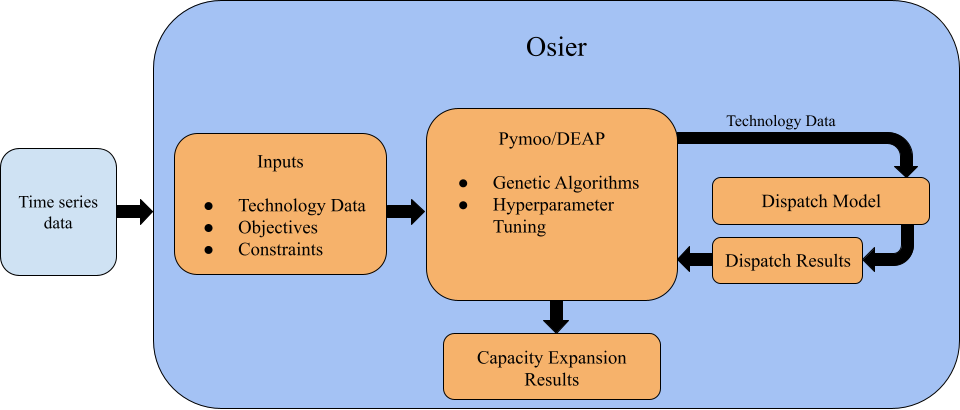
\includegraphics[width=\columnwidth]{figures/osier_flow}
    \caption{The flow of data into and within \ac{osier}}
    \label{fig:osier_flow}
\end{figure}

Technology data, objectives, constraints, and a dispatch model are all features
within \ac{osier}, while \ac{pymoo} drives the optimization of these objectives \cite{blank_pymoo_2020}.
The dispatch model is independently executable for inspecting specific test
cases and mapping solutions from other solvers onto \ac{osier}'s objective
space. The next sections elaborate on model inputs, \acfp{ga}, and the dispatch model's 
formulation.

% \textcolor{red}{This chapter is mostly written but there are a few things that
% should be added.}

\section{Inputs}

% \textcolor{red}{General thoughts:}

% Accurate input data are essential but curating data represents a challenging step in the
% modeling process. \ac{osier} attempts to lower this barrier by providing a
% variety of technology data from ``reliable'' sources.

% This section connects to the normative and descriptive portions of modeling. 

This section describes the input data and parameters that users must provide to run an \ac{osier} simulation. Broadly, \ac{osier} needs
technology data and some objectives to optimize. 

\subsection{Technology Data}
\ac{osier} only requires marginal costs and technology names in order to run successfully.
These data are needed to run the dispatch model. \ac{osier} also accepts operational data, such
as ramp rates and storage capacities. Additionally, \ac{osier} will understand any bespoke 
piece of data (e.g., ``popularity,'' ``technology-readiness score,'' or anything else) that
might be needed for a user-defined objective. All of these data are passed to \ac{osier}
through an \texttt{osier.Technology} object. Code listing \ref{listing:user-defined-technologies}
shows how users can create a simple technology object.

\begin{listing}[!ht]
    \caption{A basic technology object in \ac{osier}.}
    \label{listing:user-defined-technologies}
    \begin{minted}
    [ frame=lines, framesep=2mm, baselinestretch=1.2, bgcolor=LightGray,
    fontsize=\footnotesize, linenos ] {python} 
    from osier import ThermalTechnology

    fusion = ThermalTechnology(technology_name="Fusion",
                               dispatchable=True,
                               renewable=False,
                               fuel_cost=10*(GWh)**-1,
                               lifecycle_co2_rate=0.0,
                               )
    \end{minted}
    \end{listing}

\subsection{Objectives}
\label{section:osier_objectives}

There are many possible objectives to optimize. This section summarizes a few of
them and how they may be calculated in \ac{osier}. Due to \ac{pymoo}'s
structure, all objectives are minimized. Therefore, if users wish to maximize
some quantity, it must be reformatted with a reversal in sign to be an equivalent minimization objective.

\subsubsection{Per-unit-capacity}

Some quantities of interest depend on the \textit{capacity} of each technology.
For example, land use of different energy producers is often reported as a land
density $\text{km}^2/\text{MW}$. A generalized specific \textit{density} with respect to power 
may be $\text{unit}/\text{MW}$. The objective function for these quantities reads
\begin{align}
    \mathcal{K} &= \sum_g^G \textbf{CAP}_g \kappa_g ,
    \intertext{Where}
    \kappa &= \text{the power density of the \textit{g-th} technology} \quad \left[\frac{-}{MW}\right].
\end{align}

Table \ref{tab:objectives-per-capacity} lists some example objectives that could be
minimized or maximized.

\begin{table}[h]
    \centering
    \caption{Example objectives on a per-unit-capacity basis.}
    \begin{tabular}{cc}
       \toprule
       Quantity  & Units (per MW)\\
       \midrule
        Land Use & $\left[\text{km$^2$}\right]$\\
        Employment & $\left[\text{jobs}\right]$\\
        Capital Cost & $\left[\text{\$}\right]$\\
        Fixed O\&M Cost & $\left[\text{\$ / year}\right]$\\
        \bottomrule
    \end{tabular}
    \label{tab:objectives-per-capacity}
\end{table}

\subsubsection{Per-unit-energy}

Some quantities of interest depend on the \textit{amount of energy produced} by
each technology. For example, carbon emissions only occur when a coal or natural
gas plant burns fuel. A generalized specific \textit{intensity} with respect to energy 
may be in $\text{unit}/\text{MWh}$. The objective function for these quantities reads
\begin{align}
    \mathcal{E} &= \sum_g^G \xi_g \sum_t^T x_{g,t},
    \intertext{where}
    \xi_g &= \text{the energy density of the \textit{g-th} technology}\quad
    \left[\frac{-}{MWh}\right].
\end{align}

\begin{table}[h]
    \centering
    \caption{Example objectives on a per-unit-energy basis.}
    \begin{tabular}{cc}
       \toprule
       Quantity  & Units (per MWh)\\
       \midrule
        \acs{ghg} Emissions & $\left[\text{kg}\right]$ \\
        Water Use & $\left[\text{L}\right]$\\
        ``Safety'' & $\left[\text{deaths}\right]$\\
        Fuel Cost & $\left[\text{\$}\right]$\\
        Variable O\&M Cost & $\left[\text{\$}\right]$\\
        \bottomrule
    \end{tabular}
    \label{tab:objectives-per-energy}
\end{table}

\subsubsection{Reliability and Predictability}

Reliability has many definitions in the literature and it also depends heavily
on the dispatch method. A hierarchical flow, which dispatches energy based on a
set of rules (as opposed to true cost minimization), may simply report the
fraction of hours when electricity demand was not met by the model
\cite{donado_hyres_2020,bilil_multiobjective_2014,kamjoo_multi-objective_2016,riou_multi-objective_2021}.
\acs{lp} or \acs{milp} formulations typically have an energy balance constraint requiring 
electricity demand to be satisfied at all times, or within some specified tolerance. 
Thus reliability may be translated into a cost by determining consumers'
\ac{wtp} for electricity \cite{gorman_quest_2022, najafi_value_2021}. However,
this thesis relates system reliability to price volatility and net demand
predictability. Since the price of electricity is determined by matching supply
and demand, the price will spike when supply and demand are out of phase. For
instance, geopolitics may cause the supply of natural gas to drop, increasing
the spot price of electricity. Or, more commonly, the availability of solar and
wind resources may fall unexpectedly, leading to a greater demand for backup
energy. Both of those examples are difficult to predict; otherwise, fuel
reserves could be deployed, avoiding the price shock. Thus, I propose that
measuring the predictability and volatility of an energy system is an
appropriate proxy for reliability. Additionally, minimal price volatility is
considered an aspect of energy justice \cite{sovacool_energy_2015,
van_uffelen_revisiting_2022}.

In this thesis, I measure the  predictability of hourly electricity prices and
net demand using a measure from complexity science, \ac{wpe}
\cite{fadlallah_weighted-permutation_2013}. Permutation entropy, the precursor
to \ac{wpe}, is essentially the Shannon entropy for particular sequences of
values called \textit{motifs} \cite{bandt_permutation_2002}. \ac{wpe} expands on this
concept by weighting each instance of a motif by its variance
\cite{fadlallah_weighted-permutation_2013,garland_model-free_2014}. \ac{wpe} is
defined as
\begin{align}
    H_w(m) &= -\sum_{\pi \in \Pi} P_w(\pi)\log_2(P_w(\pi))
    \intertext{where}
    \pi &= \text{a particular motif,}\nonumber\\
    P_w &= \text{the probability of a given motif, $\pi$,}\nonumber\\
    &= \frac{\mathlarger{\sum\limits_{j\leq N}} w\left(x_j^{(m, \tau)}\right)\cdot\delta\left(\phi\left(x_j^{(m, \tau)}\right), \pi_i\right)}{\mathlarger{\sum\limits_{j\leq N}} w\left(x_j^{(m, \tau)}\right)}
    \intertext{and}
    w\left(x_j^{(m, \tau)}\right) &= \text{the weight of a particular vector}\nonumber\\
      &= \frac{1}{m}{\sum_{j}^m} \left(x_j^{(m,\tau)} - \Bar{x}\right)^2,\\\
     \phi(\cdot) &= \text{the ordinal pattern of a vector,}\nonumber\\
     \delta(\cdot) &= \text{Kronecker delta,}\nonumber\\
     m &= \text{the embedding dimension,}\nonumber\\
     \tau &= \text{the time delay}\nonumber.
\end{align}

There are other reliability metrics in the literature, frequently employing some
variation on the ``spread'' of data through standard deviation  or mean squared
error \cite{galvani_optimal_2021, galvani_unified_2014,
delsole_predictability_2004}. However, these metrics are unbounded and do not
contain any information about the underlying dynamics that produce a certain
distribution. Whereas \ac{wpe} can indicate a theoretical ceiling on
predictability \cite{garland_model-free_2014}. Importantly, \ac{wpe} works for
systems where the underlying dynamics are unknown. The Hurst exponent is another
measure of predictability, but it too has drawbacks, such as computational
expense and a stationarity requirement \cite{mesa_hurst_1993,
chandrasekaran_investigation_2019}. This thesis uses the \ac{wpe} implementation
I contributed to the open source package \texttt{PyEntropy}
\cite{donets_pyentropy_2023}.

\subsubsection{User-defined Objectives}

A key feature of \ac{osier} is the ability for users to define their own
objectives relatively easily. This feature is required
because modelers cannot know \textit{a priori} every objective that users might
be interested in optimizing. While \ac{osier} ships with some standard objective
functions, allowing users to create their own objectives makes every model
bespoke. With requisite user-supplied data \textit{any quantitative metric may be used as an objective in
\ac{osier}.} Every objective function has at least two arguments, the list of
technologies used in the model and the solved dispatch model. Users will never
have to pass these arguments manually since \ac{osier} will automatically call
the function during a simulation. One example of a user-defined objective might
be technology readiness. This objective is independent from the energy produced
and could be weighted by the capacity but is not a per-unit-capacity objective.
The values of the readiness parameter must be passed to each \texttt{Technology}
object, which can be accessed at run-time. Code listing
\ref{listing:user-defined-objective} shows the basic approach to creating a new
objective. 

\begin{listing}[!ht]
\caption{The fundamental way to create a novel objective in \ac{osier}.}
\label{listing:user-defined-objective}
\begin{minted}
[ frame=lines, framesep=2mm, baselinestretch=1.2, bgcolor=LightGray,
fontsize=\footnotesize, linenos ] {python} 

nuclear.readiness = 9
fusion.readiness = 3

technology_list = [nuclear, fusion]

def osier_objective(technology_list, solved_dispatch_model): 
    """ 
        Calculate the capacity-weighted technology readiness 
        score for this energy mix. 
    """

    total_capacity = np.array([t.capacity for t in technology_list]).sum()
    
    objective_value = np.array([t.readiness*t.capacity 
                                for t in technology_list]).sum()

    return objective_value / total_capacity
\end{minted}
\end{listing}
\noindent
Importantly, because all technologies in \ac{osier} are Python objects, users
can add attributes at will. Such as the technology readiness level as shown in
Code listing \ref{listing:user-defined-objective}. 

\subsection{Constraints}
\label{section:constraints}

Besides the physical constraints defined in Section \ref{section:dispatch_model},
\ac{osier} does not have any default constraints. This is because each
additional constraint corresponds to an additional assumption and will affect
the trade-off analysis that makes \ac{moo} so powerful. However, there are some
circumstances where the optimal solutions are still
infeasible in practice. For instance, if a community wants to determine the best
energy mix according to their unique objectives, this community might not have
the budget for even a least-cost solution because the capital requirements are
too high. Therefore, they must constrain the capital cost for their modeling
problem. Thus, \ac{osier} enables the following:
\begin{enumerate}
    \item Users may define their own constraints.
    \item Any objective function may be transformed into a constraint.
\end{enumerate}
This feature makes \ac{osier} unique among \acp{esom}.
Single-objective \acp{esom} can never account for unique situations such as the
one suggested above, nor any other bespoke considerations. In the case above,
the capital cost may constrain the problem while still minimizing the total
cost. The solutions under these conditions will have a higher total cost but
could be achievable in the near term due to meeting capital cost requirements.
\section{Genetic Algorithms}
\label{section:genetic-algorithms}

Rather than rely on \ac{lp} to model future capacity requirements, in this
thesis, \acp{ga} assume the role of investment optimizer. \acp{ga} share a
fundamental algorithmic structure, which is \cite{blank_pymoo_2020}
\begin{enumerate}
    \item \textbf{Initialize} a starting population of $N_p$ individuals, where
    each individual has a set of ``genes'' that are randomly chosen from the
    bounds of the decision variables.
    \item Each individual in the population is \textbf{evaluated} for
    ``fitness.'' 
    \item The \textbf{fittest}, $N_f$ individuals ``survive'' and persist in the
    next generation.
    \item A ``selection'' operator \textbf{chooses} among the surviving
    individuals to mate.
    \item The parents are \textbf{combined} using a ``crossover'' operator,
    thereby filling the remaining $N_p - N_f$ individuals for the next
    generation.
    \item The offspring are finally \textbf{mutated} with some probability,
    $\mu$, to improve genetic diversity.
\end{enumerate}
\noindent
Figure \ref{fig:genetic-alg} illustrates the flow of these steps applied to an
energy systems model.

\begin{figure}[ht]
        \centering
        \begin{tikzpicture}[node distance=1.7cm]
                \tikzstyle{every node}=[font=\small] \node (1) [lbblock]
                {\textbf{Create initial population\\ of capacity sets}}; \node
                (2) [lbblock, below of=1] {\textbf{Evaluate dispatch model and
                calculate objectives}}; \node (3) [lbblock, below of=2]
                {\textbf{Survival}}; \node (4) [lbblock, below of=3]
                {\textbf{Selection}}; \node (5) [lbblock, below of=4]
                {\textbf{Crossover}}; \node (6) [lbblock, below of=5]
                {\textbf{Mutation}}; \node (7) [lbblock, below of=6] {\textbf{Is
                the termination \\ criteria satisfied?}}; \node (8) [loblock,
                below of=7] {\textbf{Done}}; \draw [arrow] (1) -- (2); \draw
                [arrow] (2) -- (3); \draw [arrow] (3) -- (4); \draw [arrow] (4)
                -- (5); \draw [arrow] (5) -- (6); \draw [arrow] (6) -- (7);
                \draw [arrow] (7) -- (8); \draw [arrow] (7) -- node[anchor=east]
                {yes} (8); \draw [arrow] (7) -- ([shift={(0.5cm,0cm)}]7.east)--
                node[anchor=west] {no} ([shift={(0.5cm,0cm)}]2.east)--(2);
        \end{tikzpicture}
        \caption{The basic flow of the \ac{ga} used in this thesis.}
        \label{fig:genetic-alg}
\end{figure}

\subsection{Specific \Aclp{ga}} The variety of \acp{ga} comes from different
types of operators being applied to the selection, crossover, and mutation
steps. Section \ref{section:moo-in-energy} showed that \ac{nsga2} is a popular
genetic algorithm choice. However, this algorithm performs poorly with greater
than three objectives \cite{deb_fast_2002, seada_unified_2016}. This thesis
uses a more modern algorithm, \ac{unsga3}. \ac{unsga3} builds on its
predecessors \ac{nsga2} and \ac{nsga3} by unifying efficient solutions of mono-,
multi-, and many-objective problems in a single algorithm.


\ac{nsga2} improves on the basic \ac{ga} by introducing a more sophisticated
mating and selection algorithms. Instead of random selection, the individuals
are sorted by rank (i.e. fitness) and crowding distance in binary tournament
mating selection. The crowding distance is simply the Manhattan distance between
individuals. A greater crowding distance is desirable to preserve diversity and
since the extreme points are maximally diverse they should always persist and
are therefore assigned a crowding distance of infinity \cite{deb_fast_2002}.

The successor to \ac{nsga2}, \ac{nsga3}, enhances the many-objective
capabilities of the former by introducing reference directions. Reference
directions are used for initialization and the survival steps. In addition to
fitness, individuals are chosen based on their proximity to a reference line,
thus ensuring population diversity which greatly important for many-objective
problems. Since diversity is handled by reference directions, individuals are
selected randomly for mating. References directions are rays passing through
uniformly spaced points on the unit simplex \cite{seada_unified_2016,
blank_generating_2021}. In this thesis, I use the Riesz s- Energy method
described by Blank et al. to calculate these points for a problem with an
arbitrary number of objectives \cite{blank_generating_2021}. Figure
\ref{fig:ref-dirs} illustrates a set of initialized reference directions used
in such methods.

\begin{figure}[h]
  \centering
  \resizebox{0.6\columnwidth}{!}{%% Creator: Matplotlib, PGF backend
%%
%% To include the figure in your LaTeX document, write
%%   \input{<filename>.pgf}
%%
%% Make sure the required packages are loaded in your preamble
%%   \usepackage{pgf}
%%
%% Also ensure that all the required font packages are loaded; for instance,
%% the lmodern package is sometimes necessary when using math font.
%%   \usepackage{lmodern}
%%
%% Figures using additional raster images can only be included by \input if
%% they are in the same directory as the main LaTeX file. For loading figures
%% from other directories you can use the `import` package
%%   \usepackage{import}
%%
%% and then include the figures with
%%   \import{<path to file>}{<filename>.pgf}
%%
%% Matplotlib used the following preamble
%%   \def\mathdefault#1{#1}
%%   \everymath=\expandafter{\the\everymath\displaystyle}
%%   \IfFileExists{scrextend.sty}{
%%     \usepackage[fontsize=10.000000pt]{scrextend}
%%   }{
%%     \renewcommand{\normalsize}{\fontsize{10.000000}{12.000000}\selectfont}
%%     \normalsize
%%   }
%%   
%%   \makeatletter\@ifpackageloaded{underscore}{}{\usepackage[strings]{underscore}}\makeatother
%%
\begingroup%
\makeatletter%
\begin{pgfpicture}%
\pgfpathrectangle{\pgfpointorigin}{\pgfqpoint{6.454833in}{6.506946in}}%
\pgfusepath{use as bounding box, clip}%
\begin{pgfscope}%
\pgfsetbuttcap%
\pgfsetmiterjoin%
\definecolor{currentfill}{rgb}{1.000000,1.000000,1.000000}%
\pgfsetfillcolor{currentfill}%
\pgfsetlinewidth{0.000000pt}%
\definecolor{currentstroke}{rgb}{0.000000,0.000000,0.000000}%
\pgfsetstrokecolor{currentstroke}%
\pgfsetdash{}{0pt}%
\pgfpathmoveto{\pgfqpoint{0.000000in}{0.000000in}}%
\pgfpathlineto{\pgfqpoint{6.454833in}{0.000000in}}%
\pgfpathlineto{\pgfqpoint{6.454833in}{6.506946in}}%
\pgfpathlineto{\pgfqpoint{0.000000in}{6.506946in}}%
\pgfpathlineto{\pgfqpoint{0.000000in}{0.000000in}}%
\pgfpathclose%
\pgfusepath{fill}%
\end{pgfscope}%
\begin{pgfscope}%
\pgfsetbuttcap%
\pgfsetmiterjoin%
\definecolor{currentfill}{rgb}{1.000000,1.000000,1.000000}%
\pgfsetfillcolor{currentfill}%
\pgfsetlinewidth{0.000000pt}%
\definecolor{currentstroke}{rgb}{0.000000,0.000000,0.000000}%
\pgfsetstrokecolor{currentstroke}%
\pgfsetstrokeopacity{0.000000}%
\pgfsetdash{}{0pt}%
\pgfpathmoveto{\pgfqpoint{0.194833in}{0.246946in}}%
\pgfpathlineto{\pgfqpoint{6.354833in}{0.246946in}}%
\pgfpathlineto{\pgfqpoint{6.354833in}{6.406946in}}%
\pgfpathlineto{\pgfqpoint{0.194833in}{6.406946in}}%
\pgfpathlineto{\pgfqpoint{0.194833in}{0.246946in}}%
\pgfpathclose%
\pgfusepath{fill}%
\end{pgfscope}%
\begin{pgfscope}%
\pgfsetbuttcap%
\pgfsetmiterjoin%
\definecolor{currentfill}{rgb}{0.950000,0.950000,0.950000}%
\pgfsetfillcolor{currentfill}%
\pgfsetfillopacity{0.500000}%
\pgfsetlinewidth{1.003750pt}%
\definecolor{currentstroke}{rgb}{0.950000,0.950000,0.950000}%
\pgfsetstrokecolor{currentstroke}%
\pgfsetstrokeopacity{0.500000}%
\pgfsetdash{}{0pt}%
\pgfpathmoveto{\pgfqpoint{3.358076in}{4.263351in}}%
\pgfpathlineto{\pgfqpoint{6.075248in}{2.391249in}}%
\pgfpathlineto{\pgfqpoint{6.252387in}{4.495556in}}%
\pgfpathlineto{\pgfqpoint{3.358076in}{6.360787in}}%
\pgfusepath{stroke,fill}%
\end{pgfscope}%
\begin{pgfscope}%
\pgfsetbuttcap%
\pgfsetmiterjoin%
\definecolor{currentfill}{rgb}{0.900000,0.900000,0.900000}%
\pgfsetfillcolor{currentfill}%
\pgfsetfillopacity{0.500000}%
\pgfsetlinewidth{1.003750pt}%
\definecolor{currentstroke}{rgb}{0.900000,0.900000,0.900000}%
\pgfsetstrokecolor{currentstroke}%
\pgfsetstrokeopacity{0.500000}%
\pgfsetdash{}{0pt}%
\pgfpathmoveto{\pgfqpoint{3.358076in}{4.263351in}}%
\pgfpathlineto{\pgfqpoint{0.640904in}{2.391249in}}%
\pgfpathlineto{\pgfqpoint{0.463765in}{4.495556in}}%
\pgfpathlineto{\pgfqpoint{3.358076in}{6.360787in}}%
\pgfusepath{stroke,fill}%
\end{pgfscope}%
\begin{pgfscope}%
\pgfsetbuttcap%
\pgfsetmiterjoin%
\definecolor{currentfill}{rgb}{0.925000,0.925000,0.925000}%
\pgfsetfillcolor{currentfill}%
\pgfsetfillopacity{0.500000}%
\pgfsetlinewidth{1.003750pt}%
\definecolor{currentstroke}{rgb}{0.925000,0.925000,0.925000}%
\pgfsetstrokecolor{currentstroke}%
\pgfsetstrokeopacity{0.500000}%
\pgfsetdash{}{0pt}%
\pgfpathmoveto{\pgfqpoint{3.358076in}{4.263351in}}%
\pgfpathlineto{\pgfqpoint{0.640904in}{2.391249in}}%
\pgfpathlineto{\pgfqpoint{3.358076in}{0.289869in}}%
\pgfpathlineto{\pgfqpoint{6.075248in}{2.391249in}}%
\pgfusepath{stroke,fill}%
\end{pgfscope}%
\begin{pgfscope}%
\pgfsetbuttcap%
\pgfsetroundjoin%
\pgfsetlinewidth{0.803000pt}%
\definecolor{currentstroke}{rgb}{0.690196,0.690196,0.690196}%
\pgfsetstrokecolor{currentstroke}%
\pgfsetdash{}{0pt}%
\pgfpathmoveto{\pgfqpoint{5.911714in}{2.264777in}}%
\pgfpathlineto{\pgfqpoint{3.194029in}{4.150324in}}%
\pgfpathlineto{\pgfqpoint{3.183916in}{6.248550in}}%
\pgfusepath{stroke}%
\end{pgfscope}%
\begin{pgfscope}%
\pgfsetbuttcap%
\pgfsetroundjoin%
\pgfsetlinewidth{0.803000pt}%
\definecolor{currentstroke}{rgb}{0.690196,0.690196,0.690196}%
\pgfsetstrokecolor{currentstroke}%
\pgfsetdash{}{0pt}%
\pgfpathmoveto{\pgfqpoint{5.456913in}{1.913047in}}%
\pgfpathlineto{\pgfqpoint{2.738146in}{3.836226in}}%
\pgfpathlineto{\pgfqpoint{2.699539in}{5.936395in}}%
\pgfusepath{stroke}%
\end{pgfscope}%
\begin{pgfscope}%
\pgfsetbuttcap%
\pgfsetroundjoin%
\pgfsetlinewidth{0.803000pt}%
\definecolor{currentstroke}{rgb}{0.690196,0.690196,0.690196}%
\pgfsetstrokecolor{currentstroke}%
\pgfsetdash{}{0pt}%
\pgfpathmoveto{\pgfqpoint{4.992727in}{1.554059in}}%
\pgfpathlineto{\pgfqpoint{2.273382in}{3.516009in}}%
\pgfpathlineto{\pgfqpoint{2.205132in}{5.617775in}}%
\pgfusepath{stroke}%
\end{pgfscope}%
\begin{pgfscope}%
\pgfsetbuttcap%
\pgfsetroundjoin%
\pgfsetlinewidth{0.803000pt}%
\definecolor{currentstroke}{rgb}{0.690196,0.690196,0.690196}%
\pgfsetstrokecolor{currentstroke}%
\pgfsetdash{}{0pt}%
\pgfpathmoveto{\pgfqpoint{4.518863in}{1.187587in}}%
\pgfpathlineto{\pgfqpoint{1.799474in}{3.189491in}}%
\pgfpathlineto{\pgfqpoint{1.700378in}{5.292488in}}%
\pgfusepath{stroke}%
\end{pgfscope}%
\begin{pgfscope}%
\pgfsetbuttcap%
\pgfsetroundjoin%
\pgfsetlinewidth{0.803000pt}%
\definecolor{currentstroke}{rgb}{0.690196,0.690196,0.690196}%
\pgfsetstrokecolor{currentstroke}%
\pgfsetdash{}{0pt}%
\pgfpathmoveto{\pgfqpoint{4.035014in}{0.813393in}}%
\pgfpathlineto{\pgfqpoint{1.316148in}{2.856485in}}%
\pgfpathlineto{\pgfqpoint{1.184951in}{4.960322in}}%
\pgfusepath{stroke}%
\end{pgfscope}%
\begin{pgfscope}%
\pgfsetbuttcap%
\pgfsetroundjoin%
\pgfsetlinewidth{0.803000pt}%
\definecolor{currentstroke}{rgb}{0.690196,0.690196,0.690196}%
\pgfsetstrokecolor{currentstroke}%
\pgfsetdash{}{0pt}%
\pgfpathmoveto{\pgfqpoint{3.540863in}{0.431231in}}%
\pgfpathlineto{\pgfqpoint{0.823123in}{2.516796in}}%
\pgfpathlineto{\pgfqpoint{0.658507in}{4.621057in}}%
\pgfusepath{stroke}%
\end{pgfscope}%
\begin{pgfscope}%
\pgfsetbuttcap%
\pgfsetroundjoin%
\pgfsetlinewidth{0.803000pt}%
\definecolor{currentstroke}{rgb}{0.690196,0.690196,0.690196}%
\pgfsetstrokecolor{currentstroke}%
\pgfsetdash{}{0pt}%
\pgfpathmoveto{\pgfqpoint{3.532236in}{6.248550in}}%
\pgfpathlineto{\pgfqpoint{3.522123in}{4.150324in}}%
\pgfpathlineto{\pgfqpoint{0.804438in}{2.264777in}}%
\pgfusepath{stroke}%
\end{pgfscope}%
\begin{pgfscope}%
\pgfsetbuttcap%
\pgfsetroundjoin%
\pgfsetlinewidth{0.803000pt}%
\definecolor{currentstroke}{rgb}{0.690196,0.690196,0.690196}%
\pgfsetstrokecolor{currentstroke}%
\pgfsetdash{}{0pt}%
\pgfpathmoveto{\pgfqpoint{4.016613in}{5.936395in}}%
\pgfpathlineto{\pgfqpoint{3.978006in}{3.836226in}}%
\pgfpathlineto{\pgfqpoint{1.259239in}{1.913047in}}%
\pgfusepath{stroke}%
\end{pgfscope}%
\begin{pgfscope}%
\pgfsetbuttcap%
\pgfsetroundjoin%
\pgfsetlinewidth{0.803000pt}%
\definecolor{currentstroke}{rgb}{0.690196,0.690196,0.690196}%
\pgfsetstrokecolor{currentstroke}%
\pgfsetdash{}{0pt}%
\pgfpathmoveto{\pgfqpoint{4.511020in}{5.617775in}}%
\pgfpathlineto{\pgfqpoint{4.442770in}{3.516009in}}%
\pgfpathlineto{\pgfqpoint{1.723425in}{1.554059in}}%
\pgfusepath{stroke}%
\end{pgfscope}%
\begin{pgfscope}%
\pgfsetbuttcap%
\pgfsetroundjoin%
\pgfsetlinewidth{0.803000pt}%
\definecolor{currentstroke}{rgb}{0.690196,0.690196,0.690196}%
\pgfsetstrokecolor{currentstroke}%
\pgfsetdash{}{0pt}%
\pgfpathmoveto{\pgfqpoint{5.015774in}{5.292488in}}%
\pgfpathlineto{\pgfqpoint{4.916678in}{3.189491in}}%
\pgfpathlineto{\pgfqpoint{2.197289in}{1.187587in}}%
\pgfusepath{stroke}%
\end{pgfscope}%
\begin{pgfscope}%
\pgfsetbuttcap%
\pgfsetroundjoin%
\pgfsetlinewidth{0.803000pt}%
\definecolor{currentstroke}{rgb}{0.690196,0.690196,0.690196}%
\pgfsetstrokecolor{currentstroke}%
\pgfsetdash{}{0pt}%
\pgfpathmoveto{\pgfqpoint{5.531201in}{4.960322in}}%
\pgfpathlineto{\pgfqpoint{5.400004in}{2.856485in}}%
\pgfpathlineto{\pgfqpoint{2.681138in}{0.813393in}}%
\pgfusepath{stroke}%
\end{pgfscope}%
\begin{pgfscope}%
\pgfsetbuttcap%
\pgfsetroundjoin%
\pgfsetlinewidth{0.803000pt}%
\definecolor{currentstroke}{rgb}{0.690196,0.690196,0.690196}%
\pgfsetstrokecolor{currentstroke}%
\pgfsetdash{}{0pt}%
\pgfpathmoveto{\pgfqpoint{6.057645in}{4.621057in}}%
\pgfpathlineto{\pgfqpoint{5.893029in}{2.516796in}}%
\pgfpathlineto{\pgfqpoint{3.175289in}{0.431231in}}%
\pgfusepath{stroke}%
\end{pgfscope}%
\begin{pgfscope}%
\pgfsetbuttcap%
\pgfsetroundjoin%
\pgfsetlinewidth{0.803000pt}%
\definecolor{currentstroke}{rgb}{0.690196,0.690196,0.690196}%
\pgfsetstrokecolor{currentstroke}%
\pgfsetdash{}{0pt}%
\pgfpathmoveto{\pgfqpoint{0.630280in}{2.517456in}}%
\pgfpathlineto{\pgfqpoint{3.358076in}{4.389566in}}%
\pgfpathlineto{\pgfqpoint{6.085872in}{2.517456in}}%
\pgfusepath{stroke}%
\end{pgfscope}%
\begin{pgfscope}%
\pgfsetbuttcap%
\pgfsetroundjoin%
\pgfsetlinewidth{0.803000pt}%
\definecolor{currentstroke}{rgb}{0.690196,0.690196,0.690196}%
\pgfsetstrokecolor{currentstroke}%
\pgfsetdash{}{0pt}%
\pgfpathmoveto{\pgfqpoint{0.600709in}{2.868742in}}%
\pgfpathlineto{\pgfqpoint{3.358076in}{4.740592in}}%
\pgfpathlineto{\pgfqpoint{6.115443in}{2.868742in}}%
\pgfusepath{stroke}%
\end{pgfscope}%
\begin{pgfscope}%
\pgfsetbuttcap%
\pgfsetroundjoin%
\pgfsetlinewidth{0.803000pt}%
\definecolor{currentstroke}{rgb}{0.690196,0.690196,0.690196}%
\pgfsetstrokecolor{currentstroke}%
\pgfsetdash{}{0pt}%
\pgfpathmoveto{\pgfqpoint{0.570490in}{3.227729in}}%
\pgfpathlineto{\pgfqpoint{3.358076in}{5.098883in}}%
\pgfpathlineto{\pgfqpoint{6.145662in}{3.227729in}}%
\pgfusepath{stroke}%
\end{pgfscope}%
\begin{pgfscope}%
\pgfsetbuttcap%
\pgfsetroundjoin%
\pgfsetlinewidth{0.803000pt}%
\definecolor{currentstroke}{rgb}{0.690196,0.690196,0.690196}%
\pgfsetstrokecolor{currentstroke}%
\pgfsetdash{}{0pt}%
\pgfpathmoveto{\pgfqpoint{0.539601in}{3.594671in}}%
\pgfpathlineto{\pgfqpoint{3.358076in}{5.464666in}}%
\pgfpathlineto{\pgfqpoint{6.176551in}{3.594671in}}%
\pgfusepath{stroke}%
\end{pgfscope}%
\begin{pgfscope}%
\pgfsetbuttcap%
\pgfsetroundjoin%
\pgfsetlinewidth{0.803000pt}%
\definecolor{currentstroke}{rgb}{0.690196,0.690196,0.690196}%
\pgfsetstrokecolor{currentstroke}%
\pgfsetdash{}{0pt}%
\pgfpathmoveto{\pgfqpoint{0.508019in}{3.969836in}}%
\pgfpathlineto{\pgfqpoint{3.358076in}{5.838179in}}%
\pgfpathlineto{\pgfqpoint{6.208133in}{3.969836in}}%
\pgfusepath{stroke}%
\end{pgfscope}%
\begin{pgfscope}%
\pgfsetbuttcap%
\pgfsetroundjoin%
\pgfsetlinewidth{0.803000pt}%
\definecolor{currentstroke}{rgb}{0.690196,0.690196,0.690196}%
\pgfsetstrokecolor{currentstroke}%
\pgfsetdash{}{0pt}%
\pgfpathmoveto{\pgfqpoint{0.475722in}{4.353505in}}%
\pgfpathlineto{\pgfqpoint{3.358076in}{6.219668in}}%
\pgfpathlineto{\pgfqpoint{6.240430in}{4.353505in}}%
\pgfusepath{stroke}%
\end{pgfscope}%
\begin{pgfscope}%
\pgfsetrectcap%
\pgfsetroundjoin%
\pgfsetlinewidth{0.803000pt}%
\definecolor{currentstroke}{rgb}{0.000000,0.000000,0.000000}%
\pgfsetstrokecolor{currentstroke}%
\pgfsetdash{}{0pt}%
\pgfpathmoveto{\pgfqpoint{6.075248in}{2.391249in}}%
\pgfpathlineto{\pgfqpoint{3.358076in}{0.289869in}}%
\pgfusepath{stroke}%
\end{pgfscope}%
\begin{pgfscope}%
\pgfsetrectcap%
\pgfsetroundjoin%
\pgfsetlinewidth{0.803000pt}%
\definecolor{currentstroke}{rgb}{0.000000,0.000000,0.000000}%
\pgfsetstrokecolor{currentstroke}%
\pgfsetdash{}{0pt}%
\pgfpathmoveto{\pgfqpoint{5.888724in}{2.280728in}}%
\pgfpathlineto{\pgfqpoint{5.957758in}{2.232831in}}%
\pgfusepath{stroke}%
\end{pgfscope}%
\begin{pgfscope}%
\definecolor{textcolor}{rgb}{0.000000,0.000000,0.000000}%
\pgfsetstrokecolor{textcolor}%
\pgfsetfillcolor{textcolor}%
\pgftext[x=6.047013in,y=2.067182in,,top]{\color{textcolor}{\rmfamily\fontsize{10.000000}{12.000000}\selectfont\catcode`\^=\active\def^{\ifmmode\sp\else\^{}\fi}\catcode`\%=\active\def%{\%}$\mathdefault{0.0}$}}%
\end{pgfscope}%
\begin{pgfscope}%
\pgfsetrectcap%
\pgfsetroundjoin%
\pgfsetlinewidth{0.803000pt}%
\definecolor{currentstroke}{rgb}{0.000000,0.000000,0.000000}%
\pgfsetstrokecolor{currentstroke}%
\pgfsetdash{}{0pt}%
\pgfpathmoveto{\pgfqpoint{5.433901in}{1.929325in}}%
\pgfpathlineto{\pgfqpoint{5.503001in}{1.880446in}}%
\pgfusepath{stroke}%
\end{pgfscope}%
\begin{pgfscope}%
\definecolor{textcolor}{rgb}{0.000000,0.000000,0.000000}%
\pgfsetstrokecolor{textcolor}%
\pgfsetfillcolor{textcolor}%
\pgftext[x=5.593673in,y=1.713497in,,top]{\color{textcolor}{\rmfamily\fontsize{10.000000}{12.000000}\selectfont\catcode`\^=\active\def^{\ifmmode\sp\else\^{}\fi}\catcode`\%=\active\def%{\%}$\mathdefault{0.2}$}}%
\end{pgfscope}%
\begin{pgfscope}%
\pgfsetrectcap%
\pgfsetroundjoin%
\pgfsetlinewidth{0.803000pt}%
\definecolor{currentstroke}{rgb}{0.000000,0.000000,0.000000}%
\pgfsetstrokecolor{currentstroke}%
\pgfsetdash{}{0pt}%
\pgfpathmoveto{\pgfqpoint{4.969697in}{1.570675in}}%
\pgfpathlineto{\pgfqpoint{5.038852in}{1.520781in}}%
\pgfusepath{stroke}%
\end{pgfscope}%
\begin{pgfscope}%
\definecolor{textcolor}{rgb}{0.000000,0.000000,0.000000}%
\pgfsetstrokecolor{textcolor}%
\pgfsetfillcolor{textcolor}%
\pgftext[x=5.130981in,y=1.352515in,,top]{\color{textcolor}{\rmfamily\fontsize{10.000000}{12.000000}\selectfont\catcode`\^=\active\def^{\ifmmode\sp\else\^{}\fi}\catcode`\%=\active\def%{\%}$\mathdefault{0.4}$}}%
\end{pgfscope}%
\begin{pgfscope}%
\pgfsetrectcap%
\pgfsetroundjoin%
\pgfsetlinewidth{0.803000pt}%
\definecolor{currentstroke}{rgb}{0.000000,0.000000,0.000000}%
\pgfsetstrokecolor{currentstroke}%
\pgfsetdash{}{0pt}%
\pgfpathmoveto{\pgfqpoint{4.495819in}{1.204551in}}%
\pgfpathlineto{\pgfqpoint{4.565016in}{1.153611in}}%
\pgfusepath{stroke}%
\end{pgfscope}%
\begin{pgfscope}%
\definecolor{textcolor}{rgb}{0.000000,0.000000,0.000000}%
\pgfsetstrokecolor{textcolor}%
\pgfsetfillcolor{textcolor}%
\pgftext[x=4.658643in,y=0.984008in,,top]{\color{textcolor}{\rmfamily\fontsize{10.000000}{12.000000}\selectfont\catcode`\^=\active\def^{\ifmmode\sp\else\^{}\fi}\catcode`\%=\active\def%{\%}$\mathdefault{0.6}$}}%
\end{pgfscope}%
\begin{pgfscope}%
\pgfsetrectcap%
\pgfsetroundjoin%
\pgfsetlinewidth{0.803000pt}%
\definecolor{currentstroke}{rgb}{0.000000,0.000000,0.000000}%
\pgfsetstrokecolor{currentstroke}%
\pgfsetdash{}{0pt}%
\pgfpathmoveto{\pgfqpoint{4.011962in}{0.830716in}}%
\pgfpathlineto{\pgfqpoint{4.081186in}{0.778697in}}%
\pgfusepath{stroke}%
\end{pgfscope}%
\begin{pgfscope}%
\definecolor{textcolor}{rgb}{0.000000,0.000000,0.000000}%
\pgfsetstrokecolor{textcolor}%
\pgfsetfillcolor{textcolor}%
\pgftext[x=4.176355in,y=0.607737in,,top]{\color{textcolor}{\rmfamily\fontsize{10.000000}{12.000000}\selectfont\catcode`\^=\active\def^{\ifmmode\sp\else\^{}\fi}\catcode`\%=\active\def%{\%}$\mathdefault{0.8}$}}%
\end{pgfscope}%
\begin{pgfscope}%
\pgfsetrectcap%
\pgfsetroundjoin%
\pgfsetlinewidth{0.803000pt}%
\definecolor{currentstroke}{rgb}{0.000000,0.000000,0.000000}%
\pgfsetstrokecolor{currentstroke}%
\pgfsetdash{}{0pt}%
\pgfpathmoveto{\pgfqpoint{3.517806in}{0.448925in}}%
\pgfpathlineto{\pgfqpoint{3.587044in}{0.395792in}}%
\pgfusepath{stroke}%
\end{pgfscope}%
\begin{pgfscope}%
\definecolor{textcolor}{rgb}{0.000000,0.000000,0.000000}%
\pgfsetstrokecolor{textcolor}%
\pgfsetfillcolor{textcolor}%
\pgftext[x=3.683800in,y=0.223457in,,top]{\color{textcolor}{\rmfamily\fontsize{10.000000}{12.000000}\selectfont\catcode`\^=\active\def^{\ifmmode\sp\else\^{}\fi}\catcode`\%=\active\def%{\%}$\mathdefault{1.0}$}}%
\end{pgfscope}%
\begin{pgfscope}%
\definecolor{textcolor}{rgb}{0.000000,0.000000,0.000000}%
\pgfsetstrokecolor{textcolor}%
\pgfsetfillcolor{textcolor}%
\pgftext[x=5.059162in,y=0.931525in,,,rotate=37.717305]{\color{textcolor}{\rmfamily\fontsize{14.000000}{16.800000}\selectfont\catcode`\^=\active\def^{\ifmmode\sp\else\^{}\fi}\catcode`\%=\active\def%{\%}$f_1$}}%
\end{pgfscope}%
\begin{pgfscope}%
\pgfsetrectcap%
\pgfsetroundjoin%
\pgfsetlinewidth{0.803000pt}%
\definecolor{currentstroke}{rgb}{0.000000,0.000000,0.000000}%
\pgfsetstrokecolor{currentstroke}%
\pgfsetdash{}{0pt}%
\pgfpathmoveto{\pgfqpoint{0.640904in}{2.391249in}}%
\pgfpathlineto{\pgfqpoint{3.358076in}{0.289869in}}%
\pgfusepath{stroke}%
\end{pgfscope}%
\begin{pgfscope}%
\pgfsetrectcap%
\pgfsetroundjoin%
\pgfsetlinewidth{0.803000pt}%
\definecolor{currentstroke}{rgb}{0.000000,0.000000,0.000000}%
\pgfsetstrokecolor{currentstroke}%
\pgfsetdash{}{0pt}%
\pgfpathmoveto{\pgfqpoint{0.827428in}{2.280728in}}%
\pgfpathlineto{\pgfqpoint{0.758394in}{2.232831in}}%
\pgfusepath{stroke}%
\end{pgfscope}%
\begin{pgfscope}%
\definecolor{textcolor}{rgb}{0.000000,0.000000,0.000000}%
\pgfsetstrokecolor{textcolor}%
\pgfsetfillcolor{textcolor}%
\pgftext[x=0.669139in,y=2.067182in,,top]{\color{textcolor}{\rmfamily\fontsize{10.000000}{12.000000}\selectfont\catcode`\^=\active\def^{\ifmmode\sp\else\^{}\fi}\catcode`\%=\active\def%{\%}$\mathdefault{0.0}$}}%
\end{pgfscope}%
\begin{pgfscope}%
\pgfsetrectcap%
\pgfsetroundjoin%
\pgfsetlinewidth{0.803000pt}%
\definecolor{currentstroke}{rgb}{0.000000,0.000000,0.000000}%
\pgfsetstrokecolor{currentstroke}%
\pgfsetdash{}{0pt}%
\pgfpathmoveto{\pgfqpoint{1.282251in}{1.929325in}}%
\pgfpathlineto{\pgfqpoint{1.213151in}{1.880446in}}%
\pgfusepath{stroke}%
\end{pgfscope}%
\begin{pgfscope}%
\definecolor{textcolor}{rgb}{0.000000,0.000000,0.000000}%
\pgfsetstrokecolor{textcolor}%
\pgfsetfillcolor{textcolor}%
\pgftext[x=1.122479in,y=1.713497in,,top]{\color{textcolor}{\rmfamily\fontsize{10.000000}{12.000000}\selectfont\catcode`\^=\active\def^{\ifmmode\sp\else\^{}\fi}\catcode`\%=\active\def%{\%}$\mathdefault{0.2}$}}%
\end{pgfscope}%
\begin{pgfscope}%
\pgfsetrectcap%
\pgfsetroundjoin%
\pgfsetlinewidth{0.803000pt}%
\definecolor{currentstroke}{rgb}{0.000000,0.000000,0.000000}%
\pgfsetstrokecolor{currentstroke}%
\pgfsetdash{}{0pt}%
\pgfpathmoveto{\pgfqpoint{1.746455in}{1.570675in}}%
\pgfpathlineto{\pgfqpoint{1.677300in}{1.520781in}}%
\pgfusepath{stroke}%
\end{pgfscope}%
\begin{pgfscope}%
\definecolor{textcolor}{rgb}{0.000000,0.000000,0.000000}%
\pgfsetstrokecolor{textcolor}%
\pgfsetfillcolor{textcolor}%
\pgftext[x=1.585171in,y=1.352515in,,top]{\color{textcolor}{\rmfamily\fontsize{10.000000}{12.000000}\selectfont\catcode`\^=\active\def^{\ifmmode\sp\else\^{}\fi}\catcode`\%=\active\def%{\%}$\mathdefault{0.4}$}}%
\end{pgfscope}%
\begin{pgfscope}%
\pgfsetrectcap%
\pgfsetroundjoin%
\pgfsetlinewidth{0.803000pt}%
\definecolor{currentstroke}{rgb}{0.000000,0.000000,0.000000}%
\pgfsetstrokecolor{currentstroke}%
\pgfsetdash{}{0pt}%
\pgfpathmoveto{\pgfqpoint{2.220333in}{1.204551in}}%
\pgfpathlineto{\pgfqpoint{2.151136in}{1.153611in}}%
\pgfusepath{stroke}%
\end{pgfscope}%
\begin{pgfscope}%
\definecolor{textcolor}{rgb}{0.000000,0.000000,0.000000}%
\pgfsetstrokecolor{textcolor}%
\pgfsetfillcolor{textcolor}%
\pgftext[x=2.057509in,y=0.984008in,,top]{\color{textcolor}{\rmfamily\fontsize{10.000000}{12.000000}\selectfont\catcode`\^=\active\def^{\ifmmode\sp\else\^{}\fi}\catcode`\%=\active\def%{\%}$\mathdefault{0.6}$}}%
\end{pgfscope}%
\begin{pgfscope}%
\pgfsetrectcap%
\pgfsetroundjoin%
\pgfsetlinewidth{0.803000pt}%
\definecolor{currentstroke}{rgb}{0.000000,0.000000,0.000000}%
\pgfsetstrokecolor{currentstroke}%
\pgfsetdash{}{0pt}%
\pgfpathmoveto{\pgfqpoint{2.704190in}{0.830716in}}%
\pgfpathlineto{\pgfqpoint{2.634966in}{0.778697in}}%
\pgfusepath{stroke}%
\end{pgfscope}%
\begin{pgfscope}%
\definecolor{textcolor}{rgb}{0.000000,0.000000,0.000000}%
\pgfsetstrokecolor{textcolor}%
\pgfsetfillcolor{textcolor}%
\pgftext[x=2.539797in,y=0.607737in,,top]{\color{textcolor}{\rmfamily\fontsize{10.000000}{12.000000}\selectfont\catcode`\^=\active\def^{\ifmmode\sp\else\^{}\fi}\catcode`\%=\active\def%{\%}$\mathdefault{0.8}$}}%
\end{pgfscope}%
\begin{pgfscope}%
\pgfsetrectcap%
\pgfsetroundjoin%
\pgfsetlinewidth{0.803000pt}%
\definecolor{currentstroke}{rgb}{0.000000,0.000000,0.000000}%
\pgfsetstrokecolor{currentstroke}%
\pgfsetdash{}{0pt}%
\pgfpathmoveto{\pgfqpoint{3.198346in}{0.448925in}}%
\pgfpathlineto{\pgfqpoint{3.129108in}{0.395792in}}%
\pgfusepath{stroke}%
\end{pgfscope}%
\begin{pgfscope}%
\definecolor{textcolor}{rgb}{0.000000,0.000000,0.000000}%
\pgfsetstrokecolor{textcolor}%
\pgfsetfillcolor{textcolor}%
\pgftext[x=3.032352in,y=0.223457in,,top]{\color{textcolor}{\rmfamily\fontsize{10.000000}{12.000000}\selectfont\catcode`\^=\active\def^{\ifmmode\sp\else\^{}\fi}\catcode`\%=\active\def%{\%}$\mathdefault{1.0}$}}%
\end{pgfscope}%
\begin{pgfscope}%
\definecolor{textcolor}{rgb}{0.000000,0.000000,0.000000}%
\pgfsetstrokecolor{textcolor}%
\pgfsetfillcolor{textcolor}%
\pgftext[x=1.656990in,y=0.931525in,,,rotate=322.282695]{\color{textcolor}{\rmfamily\fontsize{14.000000}{16.800000}\selectfont\catcode`\^=\active\def^{\ifmmode\sp\else\^{}\fi}\catcode`\%=\active\def%{\%}$f_2$}}%
\end{pgfscope}%
\begin{pgfscope}%
\pgfsetrectcap%
\pgfsetroundjoin%
\pgfsetlinewidth{0.803000pt}%
\definecolor{currentstroke}{rgb}{0.000000,0.000000,0.000000}%
\pgfsetstrokecolor{currentstroke}%
\pgfsetdash{}{0pt}%
\pgfpathmoveto{\pgfqpoint{0.640904in}{2.391249in}}%
\pgfpathlineto{\pgfqpoint{0.463765in}{4.495556in}}%
\pgfusepath{stroke}%
\end{pgfscope}%
\begin{pgfscope}%
\pgfsetrectcap%
\pgfsetroundjoin%
\pgfsetlinewidth{0.803000pt}%
\definecolor{currentstroke}{rgb}{0.000000,0.000000,0.000000}%
\pgfsetstrokecolor{currentstroke}%
\pgfsetdash{}{0pt}%
\pgfpathmoveto{\pgfqpoint{0.653356in}{2.533293in}}%
\pgfpathlineto{\pgfqpoint{0.584064in}{2.485737in}}%
\pgfusepath{stroke}%
\end{pgfscope}%
\begin{pgfscope}%
\definecolor{textcolor}{rgb}{0.000000,0.000000,0.000000}%
\pgfsetstrokecolor{textcolor}%
\pgfsetfillcolor{textcolor}%
\pgftext[x=0.358681in,y=2.517456in,,top]{\color{textcolor}{\rmfamily\fontsize{10.000000}{12.000000}\selectfont\catcode`\^=\active\def^{\ifmmode\sp\else\^{}\fi}\catcode`\%=\active\def%{\%}$\mathdefault{0.0}$}}%
\end{pgfscope}%
\begin{pgfscope}%
\pgfsetrectcap%
\pgfsetroundjoin%
\pgfsetlinewidth{0.803000pt}%
\definecolor{currentstroke}{rgb}{0.000000,0.000000,0.000000}%
\pgfsetstrokecolor{currentstroke}%
\pgfsetdash{}{0pt}%
\pgfpathmoveto{\pgfqpoint{0.624048in}{2.884587in}}%
\pgfpathlineto{\pgfqpoint{0.553964in}{2.837009in}}%
\pgfusepath{stroke}%
\end{pgfscope}%
\begin{pgfscope}%
\definecolor{textcolor}{rgb}{0.000000,0.000000,0.000000}%
\pgfsetstrokecolor{textcolor}%
\pgfsetfillcolor{textcolor}%
\pgftext[x=0.326166in,y=2.868742in,,top]{\color{textcolor}{\rmfamily\fontsize{10.000000}{12.000000}\selectfont\catcode`\^=\active\def^{\ifmmode\sp\else\^{}\fi}\catcode`\%=\active\def%{\%}$\mathdefault{0.2}$}}%
\end{pgfscope}%
\begin{pgfscope}%
\pgfsetrectcap%
\pgfsetroundjoin%
\pgfsetlinewidth{0.803000pt}%
\definecolor{currentstroke}{rgb}{0.000000,0.000000,0.000000}%
\pgfsetstrokecolor{currentstroke}%
\pgfsetdash{}{0pt}%
\pgfpathmoveto{\pgfqpoint{0.594099in}{3.243577in}}%
\pgfpathlineto{\pgfqpoint{0.523203in}{3.195988in}}%
\pgfusepath{stroke}%
\end{pgfscope}%
\begin{pgfscope}%
\definecolor{textcolor}{rgb}{0.000000,0.000000,0.000000}%
\pgfsetstrokecolor{textcolor}%
\pgfsetfillcolor{textcolor}%
\pgftext[x=0.292938in,y=3.227729in,,top]{\color{textcolor}{\rmfamily\fontsize{10.000000}{12.000000}\selectfont\catcode`\^=\active\def^{\ifmmode\sp\else\^{}\fi}\catcode`\%=\active\def%{\%}$\mathdefault{0.4}$}}%
\end{pgfscope}%
\begin{pgfscope}%
\pgfsetrectcap%
\pgfsetroundjoin%
\pgfsetlinewidth{0.803000pt}%
\definecolor{currentstroke}{rgb}{0.000000,0.000000,0.000000}%
\pgfsetstrokecolor{currentstroke}%
\pgfsetdash{}{0pt}%
\pgfpathmoveto{\pgfqpoint{0.563487in}{3.610519in}}%
\pgfpathlineto{\pgfqpoint{0.491760in}{3.562930in}}%
\pgfusepath{stroke}%
\end{pgfscope}%
\begin{pgfscope}%
\definecolor{textcolor}{rgb}{0.000000,0.000000,0.000000}%
\pgfsetstrokecolor{textcolor}%
\pgfsetfillcolor{textcolor}%
\pgftext[x=0.258973in,y=3.594671in,,top]{\color{textcolor}{\rmfamily\fontsize{10.000000}{12.000000}\selectfont\catcode`\^=\active\def^{\ifmmode\sp\else\^{}\fi}\catcode`\%=\active\def%{\%}$\mathdefault{0.6}$}}%
\end{pgfscope}%
\begin{pgfscope}%
\pgfsetrectcap%
\pgfsetroundjoin%
\pgfsetlinewidth{0.803000pt}%
\definecolor{currentstroke}{rgb}{0.000000,0.000000,0.000000}%
\pgfsetstrokecolor{currentstroke}%
\pgfsetdash{}{0pt}%
\pgfpathmoveto{\pgfqpoint{0.532188in}{3.985680in}}%
\pgfpathlineto{\pgfqpoint{0.459612in}{3.938103in}}%
\pgfusepath{stroke}%
\end{pgfscope}%
\begin{pgfscope}%
\definecolor{textcolor}{rgb}{0.000000,0.000000,0.000000}%
\pgfsetstrokecolor{textcolor}%
\pgfsetfillcolor{textcolor}%
\pgftext[x=0.224248in,y=3.969836in,,top]{\color{textcolor}{\rmfamily\fontsize{10.000000}{12.000000}\selectfont\catcode`\^=\active\def^{\ifmmode\sp\else\^{}\fi}\catcode`\%=\active\def%{\%}$\mathdefault{0.8}$}}%
\end{pgfscope}%
\begin{pgfscope}%
\pgfsetrectcap%
\pgfsetroundjoin%
\pgfsetlinewidth{0.803000pt}%
\definecolor{currentstroke}{rgb}{0.000000,0.000000,0.000000}%
\pgfsetstrokecolor{currentstroke}%
\pgfsetdash{}{0pt}%
\pgfpathmoveto{\pgfqpoint{0.500181in}{4.369340in}}%
\pgfpathlineto{\pgfqpoint{0.426734in}{4.321787in}}%
\pgfusepath{stroke}%
\end{pgfscope}%
\begin{pgfscope}%
\definecolor{textcolor}{rgb}{0.000000,0.000000,0.000000}%
\pgfsetstrokecolor{textcolor}%
\pgfsetfillcolor{textcolor}%
\pgftext[x=0.188735in,y=4.353505in,,top]{\color{textcolor}{\rmfamily\fontsize{10.000000}{12.000000}\selectfont\catcode`\^=\active\def^{\ifmmode\sp\else\^{}\fi}\catcode`\%=\active\def%{\%}$\mathdefault{1.0}$}}%
\end{pgfscope}%
\begin{pgfscope}%
\definecolor{textcolor}{rgb}{0.000000,0.000000,0.000000}%
\pgfsetstrokecolor{textcolor}%
\pgfsetfillcolor{textcolor}%
\pgftext[x=-0.051568in,y=3.410189in,,,rotate=274.811779]{\color{textcolor}{\rmfamily\fontsize{14.000000}{16.800000}\selectfont\catcode`\^=\active\def^{\ifmmode\sp\else\^{}\fi}\catcode`\%=\active\def%{\%}$f_3$}}%
\end{pgfscope}%
\begin{pgfscope}%
\pgfpathrectangle{\pgfqpoint{0.194833in}{0.246946in}}{\pgfqpoint{6.160000in}{6.160000in}}%
\pgfusepath{clip}%
\pgfsetbuttcap%
\pgfsetroundjoin%
\definecolor{currentfill}{rgb}{0.121569,0.466667,0.705882}%
\pgfsetfillcolor{currentfill}%
\pgfsetlinewidth{1.003750pt}%
\definecolor{currentstroke}{rgb}{0.121569,0.466667,0.705882}%
\pgfsetstrokecolor{currentstroke}%
\pgfsetdash{}{0pt}%
\pgfpathmoveto{\pgfqpoint{0.977454in}{2.468351in}}%
\pgfpathcurveto{\pgfqpoint{0.990477in}{2.468351in}}{\pgfqpoint{1.002968in}{2.473525in}}{\pgfqpoint{1.012176in}{2.482733in}}%
\pgfpathcurveto{\pgfqpoint{1.021385in}{2.491942in}}{\pgfqpoint{1.026559in}{2.504433in}}{\pgfqpoint{1.026559in}{2.517456in}}%
\pgfpathcurveto{\pgfqpoint{1.026559in}{2.530478in}}{\pgfqpoint{1.021385in}{2.542969in}}{\pgfqpoint{1.012176in}{2.552178in}}%
\pgfpathcurveto{\pgfqpoint{1.002968in}{2.561386in}}{\pgfqpoint{0.990477in}{2.566560in}}{\pgfqpoint{0.977454in}{2.566560in}}%
\pgfpathcurveto{\pgfqpoint{0.964431in}{2.566560in}}{\pgfqpoint{0.951940in}{2.561386in}}{\pgfqpoint{0.942732in}{2.552178in}}%
\pgfpathcurveto{\pgfqpoint{0.933523in}{2.542969in}}{\pgfqpoint{0.928349in}{2.530478in}}{\pgfqpoint{0.928349in}{2.517456in}}%
\pgfpathcurveto{\pgfqpoint{0.928349in}{2.504433in}}{\pgfqpoint{0.933523in}{2.491942in}}{\pgfqpoint{0.942732in}{2.482733in}}%
\pgfpathcurveto{\pgfqpoint{0.951940in}{2.473525in}}{\pgfqpoint{0.964431in}{2.468351in}}{\pgfqpoint{0.977454in}{2.468351in}}%
\pgfpathlineto{\pgfqpoint{0.977454in}{2.468351in}}%
\pgfpathclose%
\pgfusepath{stroke,fill}%
\end{pgfscope}%
\begin{pgfscope}%
\pgfpathrectangle{\pgfqpoint{0.194833in}{0.246946in}}{\pgfqpoint{6.160000in}{6.160000in}}%
\pgfusepath{clip}%
\pgfsetbuttcap%
\pgfsetroundjoin%
\definecolor{currentfill}{rgb}{0.121569,0.466667,0.705882}%
\pgfsetfillcolor{currentfill}%
\pgfsetlinewidth{1.003750pt}%
\definecolor{currentstroke}{rgb}{0.121569,0.466667,0.705882}%
\pgfsetstrokecolor{currentstroke}%
\pgfsetdash{}{0pt}%
\pgfpathmoveto{\pgfqpoint{2.279284in}{2.468351in}}%
\pgfpathcurveto{\pgfqpoint{2.292306in}{2.468351in}}{\pgfqpoint{2.304797in}{2.473525in}}{\pgfqpoint{2.314006in}{2.482733in}}%
\pgfpathcurveto{\pgfqpoint{2.323214in}{2.491942in}}{\pgfqpoint{2.328388in}{2.504433in}}{\pgfqpoint{2.328388in}{2.517456in}}%
\pgfpathcurveto{\pgfqpoint{2.328388in}{2.530478in}}{\pgfqpoint{2.323214in}{2.542969in}}{\pgfqpoint{2.314006in}{2.552178in}}%
\pgfpathcurveto{\pgfqpoint{2.304797in}{2.561386in}}{\pgfqpoint{2.292306in}{2.566560in}}{\pgfqpoint{2.279284in}{2.566560in}}%
\pgfpathcurveto{\pgfqpoint{2.266261in}{2.566560in}}{\pgfqpoint{2.253770in}{2.561386in}}{\pgfqpoint{2.244561in}{2.552178in}}%
\pgfpathcurveto{\pgfqpoint{2.235353in}{2.542969in}}{\pgfqpoint{2.230179in}{2.530478in}}{\pgfqpoint{2.230179in}{2.517456in}}%
\pgfpathcurveto{\pgfqpoint{2.230179in}{2.504433in}}{\pgfqpoint{2.235353in}{2.491942in}}{\pgfqpoint{2.244561in}{2.482733in}}%
\pgfpathcurveto{\pgfqpoint{2.253770in}{2.473525in}}{\pgfqpoint{2.266261in}{2.468351in}}{\pgfqpoint{2.279284in}{2.468351in}}%
\pgfpathlineto{\pgfqpoint{2.279284in}{2.468351in}}%
\pgfpathclose%
\pgfusepath{stroke,fill}%
\end{pgfscope}%
\begin{pgfscope}%
\pgfpathrectangle{\pgfqpoint{0.194833in}{0.246946in}}{\pgfqpoint{6.160000in}{6.160000in}}%
\pgfusepath{clip}%
\pgfsetbuttcap%
\pgfsetroundjoin%
\definecolor{currentfill}{rgb}{0.121569,0.466667,0.705882}%
\pgfsetfillcolor{currentfill}%
\pgfsetlinewidth{1.003750pt}%
\definecolor{currentstroke}{rgb}{0.121569,0.466667,0.705882}%
\pgfsetstrokecolor{currentstroke}%
\pgfsetdash{}{0pt}%
\pgfpathmoveto{\pgfqpoint{4.461082in}{2.468351in}}%
\pgfpathcurveto{\pgfqpoint{4.474105in}{2.468351in}}{\pgfqpoint{4.486596in}{2.473525in}}{\pgfqpoint{4.495804in}{2.482733in}}%
\pgfpathcurveto{\pgfqpoint{4.505013in}{2.491942in}}{\pgfqpoint{4.510187in}{2.504433in}}{\pgfqpoint{4.510187in}{2.517456in}}%
\pgfpathcurveto{\pgfqpoint{4.510187in}{2.530478in}}{\pgfqpoint{4.505013in}{2.542969in}}{\pgfqpoint{4.495804in}{2.552178in}}%
\pgfpathcurveto{\pgfqpoint{4.486596in}{2.561386in}}{\pgfqpoint{4.474105in}{2.566560in}}{\pgfqpoint{4.461082in}{2.566560in}}%
\pgfpathcurveto{\pgfqpoint{4.448059in}{2.566560in}}{\pgfqpoint{4.435568in}{2.561386in}}{\pgfqpoint{4.426360in}{2.552178in}}%
\pgfpathcurveto{\pgfqpoint{4.417151in}{2.542969in}}{\pgfqpoint{4.411977in}{2.530478in}}{\pgfqpoint{4.411977in}{2.517456in}}%
\pgfpathcurveto{\pgfqpoint{4.411977in}{2.504433in}}{\pgfqpoint{4.417151in}{2.491942in}}{\pgfqpoint{4.426360in}{2.482733in}}%
\pgfpathcurveto{\pgfqpoint{4.435568in}{2.473525in}}{\pgfqpoint{4.448059in}{2.468351in}}{\pgfqpoint{4.461082in}{2.468351in}}%
\pgfpathlineto{\pgfqpoint{4.461082in}{2.468351in}}%
\pgfpathclose%
\pgfusepath{stroke,fill}%
\end{pgfscope}%
\begin{pgfscope}%
\pgfpathrectangle{\pgfqpoint{0.194833in}{0.246946in}}{\pgfqpoint{6.160000in}{6.160000in}}%
\pgfusepath{clip}%
\pgfsetbuttcap%
\pgfsetroundjoin%
\definecolor{currentfill}{rgb}{0.121569,0.466667,0.705882}%
\pgfsetfillcolor{currentfill}%
\pgfsetlinewidth{1.003750pt}%
\definecolor{currentstroke}{rgb}{0.121569,0.466667,0.705882}%
\pgfsetstrokecolor{currentstroke}%
\pgfsetdash{}{0pt}%
\pgfpathmoveto{\pgfqpoint{4.885244in}{2.468351in}}%
\pgfpathcurveto{\pgfqpoint{4.898267in}{2.468351in}}{\pgfqpoint{4.910758in}{2.473525in}}{\pgfqpoint{4.919967in}{2.482733in}}%
\pgfpathcurveto{\pgfqpoint{4.929175in}{2.491942in}}{\pgfqpoint{4.934349in}{2.504433in}}{\pgfqpoint{4.934349in}{2.517456in}}%
\pgfpathcurveto{\pgfqpoint{4.934349in}{2.530478in}}{\pgfqpoint{4.929175in}{2.542969in}}{\pgfqpoint{4.919967in}{2.552178in}}%
\pgfpathcurveto{\pgfqpoint{4.910758in}{2.561386in}}{\pgfqpoint{4.898267in}{2.566560in}}{\pgfqpoint{4.885244in}{2.566560in}}%
\pgfpathcurveto{\pgfqpoint{4.872222in}{2.566560in}}{\pgfqpoint{4.859731in}{2.561386in}}{\pgfqpoint{4.850522in}{2.552178in}}%
\pgfpathcurveto{\pgfqpoint{4.841314in}{2.542969in}}{\pgfqpoint{4.836140in}{2.530478in}}{\pgfqpoint{4.836140in}{2.517456in}}%
\pgfpathcurveto{\pgfqpoint{4.836140in}{2.504433in}}{\pgfqpoint{4.841314in}{2.491942in}}{\pgfqpoint{4.850522in}{2.482733in}}%
\pgfpathcurveto{\pgfqpoint{4.859731in}{2.473525in}}{\pgfqpoint{4.872222in}{2.468351in}}{\pgfqpoint{4.885244in}{2.468351in}}%
\pgfpathlineto{\pgfqpoint{4.885244in}{2.468351in}}%
\pgfpathclose%
\pgfusepath{stroke,fill}%
\end{pgfscope}%
\begin{pgfscope}%
\pgfpathrectangle{\pgfqpoint{0.194833in}{0.246946in}}{\pgfqpoint{6.160000in}{6.160000in}}%
\pgfusepath{clip}%
\pgfsetbuttcap%
\pgfsetroundjoin%
\definecolor{currentfill}{rgb}{0.121569,0.466667,0.705882}%
\pgfsetfillcolor{currentfill}%
\pgfsetlinewidth{1.003750pt}%
\definecolor{currentstroke}{rgb}{0.121569,0.466667,0.705882}%
\pgfsetstrokecolor{currentstroke}%
\pgfsetdash{}{0pt}%
\pgfpathmoveto{\pgfqpoint{4.080163in}{2.468351in}}%
\pgfpathcurveto{\pgfqpoint{4.093185in}{2.468351in}}{\pgfqpoint{4.105676in}{2.473525in}}{\pgfqpoint{4.114885in}{2.482733in}}%
\pgfpathcurveto{\pgfqpoint{4.124093in}{2.491942in}}{\pgfqpoint{4.129267in}{2.504433in}}{\pgfqpoint{4.129267in}{2.517456in}}%
\pgfpathcurveto{\pgfqpoint{4.129267in}{2.530478in}}{\pgfqpoint{4.124093in}{2.542969in}}{\pgfqpoint{4.114885in}{2.552178in}}%
\pgfpathcurveto{\pgfqpoint{4.105676in}{2.561386in}}{\pgfqpoint{4.093185in}{2.566560in}}{\pgfqpoint{4.080163in}{2.566560in}}%
\pgfpathcurveto{\pgfqpoint{4.067140in}{2.566560in}}{\pgfqpoint{4.054649in}{2.561386in}}{\pgfqpoint{4.045440in}{2.552178in}}%
\pgfpathcurveto{\pgfqpoint{4.036232in}{2.542969in}}{\pgfqpoint{4.031058in}{2.530478in}}{\pgfqpoint{4.031058in}{2.517456in}}%
\pgfpathcurveto{\pgfqpoint{4.031058in}{2.504433in}}{\pgfqpoint{4.036232in}{2.491942in}}{\pgfqpoint{4.045440in}{2.482733in}}%
\pgfpathcurveto{\pgfqpoint{4.054649in}{2.473525in}}{\pgfqpoint{4.067140in}{2.468351in}}{\pgfqpoint{4.080163in}{2.468351in}}%
\pgfpathlineto{\pgfqpoint{4.080163in}{2.468351in}}%
\pgfpathclose%
\pgfusepath{stroke,fill}%
\end{pgfscope}%
\begin{pgfscope}%
\pgfpathrectangle{\pgfqpoint{0.194833in}{0.246946in}}{\pgfqpoint{6.160000in}{6.160000in}}%
\pgfusepath{clip}%
\pgfsetbuttcap%
\pgfsetroundjoin%
\definecolor{currentfill}{rgb}{0.121569,0.466667,0.705882}%
\pgfsetfillcolor{currentfill}%
\pgfsetlinewidth{1.003750pt}%
\definecolor{currentstroke}{rgb}{0.121569,0.466667,0.705882}%
\pgfsetstrokecolor{currentstroke}%
\pgfsetdash{}{0pt}%
\pgfpathmoveto{\pgfqpoint{5.316558in}{2.468351in}}%
\pgfpathcurveto{\pgfqpoint{5.329581in}{2.468351in}}{\pgfqpoint{5.342072in}{2.473525in}}{\pgfqpoint{5.351280in}{2.482733in}}%
\pgfpathcurveto{\pgfqpoint{5.360488in}{2.491942in}}{\pgfqpoint{5.365662in}{2.504433in}}{\pgfqpoint{5.365662in}{2.517456in}}%
\pgfpathcurveto{\pgfqpoint{5.365662in}{2.530478in}}{\pgfqpoint{5.360488in}{2.542969in}}{\pgfqpoint{5.351280in}{2.552178in}}%
\pgfpathcurveto{\pgfqpoint{5.342072in}{2.561386in}}{\pgfqpoint{5.329581in}{2.566560in}}{\pgfqpoint{5.316558in}{2.566560in}}%
\pgfpathcurveto{\pgfqpoint{5.303535in}{2.566560in}}{\pgfqpoint{5.291044in}{2.561386in}}{\pgfqpoint{5.281836in}{2.552178in}}%
\pgfpathcurveto{\pgfqpoint{5.272627in}{2.542969in}}{\pgfqpoint{5.267453in}{2.530478in}}{\pgfqpoint{5.267453in}{2.517456in}}%
\pgfpathcurveto{\pgfqpoint{5.267453in}{2.504433in}}{\pgfqpoint{5.272627in}{2.491942in}}{\pgfqpoint{5.281836in}{2.482733in}}%
\pgfpathcurveto{\pgfqpoint{5.291044in}{2.473525in}}{\pgfqpoint{5.303535in}{2.468351in}}{\pgfqpoint{5.316558in}{2.468351in}}%
\pgfpathlineto{\pgfqpoint{5.316558in}{2.468351in}}%
\pgfpathclose%
\pgfusepath{stroke,fill}%
\end{pgfscope}%
\begin{pgfscope}%
\pgfpathrectangle{\pgfqpoint{0.194833in}{0.246946in}}{\pgfqpoint{6.160000in}{6.160000in}}%
\pgfusepath{clip}%
\pgfsetbuttcap%
\pgfsetroundjoin%
\definecolor{currentfill}{rgb}{0.121569,0.466667,0.705882}%
\pgfsetfillcolor{currentfill}%
\pgfsetlinewidth{1.003750pt}%
\definecolor{currentstroke}{rgb}{0.121569,0.466667,0.705882}%
\pgfsetstrokecolor{currentstroke}%
\pgfsetdash{}{0pt}%
\pgfpathmoveto{\pgfqpoint{3.654994in}{2.468351in}}%
\pgfpathcurveto{\pgfqpoint{3.668016in}{2.468351in}}{\pgfqpoint{3.680507in}{2.473525in}}{\pgfqpoint{3.689716in}{2.482733in}}%
\pgfpathcurveto{\pgfqpoint{3.698924in}{2.491942in}}{\pgfqpoint{3.704098in}{2.504433in}}{\pgfqpoint{3.704098in}{2.517456in}}%
\pgfpathcurveto{\pgfqpoint{3.704098in}{2.530478in}}{\pgfqpoint{3.698924in}{2.542969in}}{\pgfqpoint{3.689716in}{2.552178in}}%
\pgfpathcurveto{\pgfqpoint{3.680507in}{2.561386in}}{\pgfqpoint{3.668016in}{2.566560in}}{\pgfqpoint{3.654994in}{2.566560in}}%
\pgfpathcurveto{\pgfqpoint{3.641971in}{2.566560in}}{\pgfqpoint{3.629480in}{2.561386in}}{\pgfqpoint{3.620271in}{2.552178in}}%
\pgfpathcurveto{\pgfqpoint{3.611063in}{2.542969in}}{\pgfqpoint{3.605889in}{2.530478in}}{\pgfqpoint{3.605889in}{2.517456in}}%
\pgfpathcurveto{\pgfqpoint{3.605889in}{2.504433in}}{\pgfqpoint{3.611063in}{2.491942in}}{\pgfqpoint{3.620271in}{2.482733in}}%
\pgfpathcurveto{\pgfqpoint{3.629480in}{2.473525in}}{\pgfqpoint{3.641971in}{2.468351in}}{\pgfqpoint{3.654994in}{2.468351in}}%
\pgfpathlineto{\pgfqpoint{3.654994in}{2.468351in}}%
\pgfpathclose%
\pgfusepath{stroke,fill}%
\end{pgfscope}%
\begin{pgfscope}%
\pgfpathrectangle{\pgfqpoint{0.194833in}{0.246946in}}{\pgfqpoint{6.160000in}{6.160000in}}%
\pgfusepath{clip}%
\pgfsetbuttcap%
\pgfsetroundjoin%
\definecolor{currentfill}{rgb}{0.121569,0.466667,0.705882}%
\pgfsetfillcolor{currentfill}%
\pgfsetlinewidth{1.003750pt}%
\definecolor{currentstroke}{rgb}{0.121569,0.466667,0.705882}%
\pgfsetstrokecolor{currentstroke}%
\pgfsetdash{}{0pt}%
\pgfpathmoveto{\pgfqpoint{3.208301in}{2.468351in}}%
\pgfpathcurveto{\pgfqpoint{3.221323in}{2.468351in}}{\pgfqpoint{3.233815in}{2.473525in}}{\pgfqpoint{3.243023in}{2.482733in}}%
\pgfpathcurveto{\pgfqpoint{3.252231in}{2.491942in}}{\pgfqpoint{3.257405in}{2.504433in}}{\pgfqpoint{3.257405in}{2.517456in}}%
\pgfpathcurveto{\pgfqpoint{3.257405in}{2.530478in}}{\pgfqpoint{3.252231in}{2.542969in}}{\pgfqpoint{3.243023in}{2.552178in}}%
\pgfpathcurveto{\pgfqpoint{3.233815in}{2.561386in}}{\pgfqpoint{3.221323in}{2.566560in}}{\pgfqpoint{3.208301in}{2.566560in}}%
\pgfpathcurveto{\pgfqpoint{3.195278in}{2.566560in}}{\pgfqpoint{3.182787in}{2.561386in}}{\pgfqpoint{3.173579in}{2.552178in}}%
\pgfpathcurveto{\pgfqpoint{3.164370in}{2.542969in}}{\pgfqpoint{3.159196in}{2.530478in}}{\pgfqpoint{3.159196in}{2.517456in}}%
\pgfpathcurveto{\pgfqpoint{3.159196in}{2.504433in}}{\pgfqpoint{3.164370in}{2.491942in}}{\pgfqpoint{3.173579in}{2.482733in}}%
\pgfpathcurveto{\pgfqpoint{3.182787in}{2.473525in}}{\pgfqpoint{3.195278in}{2.468351in}}{\pgfqpoint{3.208301in}{2.468351in}}%
\pgfpathlineto{\pgfqpoint{3.208301in}{2.468351in}}%
\pgfpathclose%
\pgfusepath{stroke,fill}%
\end{pgfscope}%
\begin{pgfscope}%
\pgfpathrectangle{\pgfqpoint{0.194833in}{0.246946in}}{\pgfqpoint{6.160000in}{6.160000in}}%
\pgfusepath{clip}%
\pgfsetbuttcap%
\pgfsetroundjoin%
\definecolor{currentfill}{rgb}{0.121569,0.466667,0.705882}%
\pgfsetfillcolor{currentfill}%
\pgfsetlinewidth{1.003750pt}%
\definecolor{currentstroke}{rgb}{0.121569,0.466667,0.705882}%
\pgfsetstrokecolor{currentstroke}%
\pgfsetdash{}{0pt}%
\pgfpathmoveto{\pgfqpoint{2.712527in}{2.468351in}}%
\pgfpathcurveto{\pgfqpoint{2.725550in}{2.468351in}}{\pgfqpoint{2.738041in}{2.473525in}}{\pgfqpoint{2.747250in}{2.482733in}}%
\pgfpathcurveto{\pgfqpoint{2.756458in}{2.491942in}}{\pgfqpoint{2.761632in}{2.504433in}}{\pgfqpoint{2.761632in}{2.517456in}}%
\pgfpathcurveto{\pgfqpoint{2.761632in}{2.530478in}}{\pgfqpoint{2.756458in}{2.542969in}}{\pgfqpoint{2.747250in}{2.552178in}}%
\pgfpathcurveto{\pgfqpoint{2.738041in}{2.561386in}}{\pgfqpoint{2.725550in}{2.566560in}}{\pgfqpoint{2.712527in}{2.566560in}}%
\pgfpathcurveto{\pgfqpoint{2.699505in}{2.566560in}}{\pgfqpoint{2.687014in}{2.561386in}}{\pgfqpoint{2.677805in}{2.552178in}}%
\pgfpathcurveto{\pgfqpoint{2.668597in}{2.542969in}}{\pgfqpoint{2.663423in}{2.530478in}}{\pgfqpoint{2.663423in}{2.517456in}}%
\pgfpathcurveto{\pgfqpoint{2.663423in}{2.504433in}}{\pgfqpoint{2.668597in}{2.491942in}}{\pgfqpoint{2.677805in}{2.482733in}}%
\pgfpathcurveto{\pgfqpoint{2.687014in}{2.473525in}}{\pgfqpoint{2.699505in}{2.468351in}}{\pgfqpoint{2.712527in}{2.468351in}}%
\pgfpathlineto{\pgfqpoint{2.712527in}{2.468351in}}%
\pgfpathclose%
\pgfusepath{stroke,fill}%
\end{pgfscope}%
\begin{pgfscope}%
\pgfpathrectangle{\pgfqpoint{0.194833in}{0.246946in}}{\pgfqpoint{6.160000in}{6.160000in}}%
\pgfusepath{clip}%
\pgfsetbuttcap%
\pgfsetroundjoin%
\definecolor{currentfill}{rgb}{0.121569,0.466667,0.705882}%
\pgfsetfillcolor{currentfill}%
\pgfsetlinewidth{1.003750pt}%
\definecolor{currentstroke}{rgb}{0.121569,0.466667,0.705882}%
\pgfsetstrokecolor{currentstroke}%
\pgfsetdash{}{0pt}%
\pgfpathmoveto{\pgfqpoint{5.738698in}{2.468351in}}%
\pgfpathcurveto{\pgfqpoint{5.751721in}{2.468351in}}{\pgfqpoint{5.764212in}{2.473525in}}{\pgfqpoint{5.773420in}{2.482733in}}%
\pgfpathcurveto{\pgfqpoint{5.782629in}{2.491942in}}{\pgfqpoint{5.787803in}{2.504433in}}{\pgfqpoint{5.787803in}{2.517456in}}%
\pgfpathcurveto{\pgfqpoint{5.787803in}{2.530478in}}{\pgfqpoint{5.782629in}{2.542969in}}{\pgfqpoint{5.773420in}{2.552178in}}%
\pgfpathcurveto{\pgfqpoint{5.764212in}{2.561386in}}{\pgfqpoint{5.751721in}{2.566560in}}{\pgfqpoint{5.738698in}{2.566560in}}%
\pgfpathcurveto{\pgfqpoint{5.725675in}{2.566560in}}{\pgfqpoint{5.713184in}{2.561386in}}{\pgfqpoint{5.703976in}{2.552178in}}%
\pgfpathcurveto{\pgfqpoint{5.694767in}{2.542969in}}{\pgfqpoint{5.689593in}{2.530478in}}{\pgfqpoint{5.689593in}{2.517456in}}%
\pgfpathcurveto{\pgfqpoint{5.689593in}{2.504433in}}{\pgfqpoint{5.694767in}{2.491942in}}{\pgfqpoint{5.703976in}{2.482733in}}%
\pgfpathcurveto{\pgfqpoint{5.713184in}{2.473525in}}{\pgfqpoint{5.725675in}{2.468351in}}{\pgfqpoint{5.738698in}{2.468351in}}%
\pgfpathlineto{\pgfqpoint{5.738698in}{2.468351in}}%
\pgfpathclose%
\pgfusepath{stroke,fill}%
\end{pgfscope}%
\begin{pgfscope}%
\pgfpathrectangle{\pgfqpoint{0.194833in}{0.246946in}}{\pgfqpoint{6.160000in}{6.160000in}}%
\pgfusepath{clip}%
\pgfsetbuttcap%
\pgfsetroundjoin%
\definecolor{currentfill}{rgb}{0.121569,0.466667,0.705882}%
\pgfsetfillcolor{currentfill}%
\pgfsetlinewidth{1.003750pt}%
\definecolor{currentstroke}{rgb}{0.121569,0.466667,0.705882}%
\pgfsetstrokecolor{currentstroke}%
\pgfsetdash{}{0pt}%
\pgfpathmoveto{\pgfqpoint{1.433009in}{2.468351in}}%
\pgfpathcurveto{\pgfqpoint{1.446031in}{2.468351in}}{\pgfqpoint{1.458522in}{2.473525in}}{\pgfqpoint{1.467731in}{2.482733in}}%
\pgfpathcurveto{\pgfqpoint{1.476939in}{2.491942in}}{\pgfqpoint{1.482113in}{2.504433in}}{\pgfqpoint{1.482113in}{2.517456in}}%
\pgfpathcurveto{\pgfqpoint{1.482113in}{2.530478in}}{\pgfqpoint{1.476939in}{2.542969in}}{\pgfqpoint{1.467731in}{2.552178in}}%
\pgfpathcurveto{\pgfqpoint{1.458522in}{2.561386in}}{\pgfqpoint{1.446031in}{2.566560in}}{\pgfqpoint{1.433009in}{2.566560in}}%
\pgfpathcurveto{\pgfqpoint{1.419986in}{2.566560in}}{\pgfqpoint{1.407495in}{2.561386in}}{\pgfqpoint{1.398286in}{2.552178in}}%
\pgfpathcurveto{\pgfqpoint{1.389078in}{2.542969in}}{\pgfqpoint{1.383904in}{2.530478in}}{\pgfqpoint{1.383904in}{2.517456in}}%
\pgfpathcurveto{\pgfqpoint{1.383904in}{2.504433in}}{\pgfqpoint{1.389078in}{2.491942in}}{\pgfqpoint{1.398286in}{2.482733in}}%
\pgfpathcurveto{\pgfqpoint{1.407495in}{2.473525in}}{\pgfqpoint{1.419986in}{2.468351in}}{\pgfqpoint{1.433009in}{2.468351in}}%
\pgfpathlineto{\pgfqpoint{1.433009in}{2.468351in}}%
\pgfpathclose%
\pgfusepath{stroke,fill}%
\end{pgfscope}%
\begin{pgfscope}%
\pgfpathrectangle{\pgfqpoint{0.194833in}{0.246946in}}{\pgfqpoint{6.160000in}{6.160000in}}%
\pgfusepath{clip}%
\pgfsetbuttcap%
\pgfsetroundjoin%
\definecolor{currentfill}{rgb}{0.121569,0.466667,0.705882}%
\pgfsetfillcolor{currentfill}%
\pgfsetlinewidth{1.003750pt}%
\definecolor{currentstroke}{rgb}{0.121569,0.466667,0.705882}%
\pgfsetstrokecolor{currentstroke}%
\pgfsetdash{}{0pt}%
\pgfpathmoveto{\pgfqpoint{1.868054in}{2.468351in}}%
\pgfpathcurveto{\pgfqpoint{1.881077in}{2.468351in}}{\pgfqpoint{1.893568in}{2.473525in}}{\pgfqpoint{1.902776in}{2.482733in}}%
\pgfpathcurveto{\pgfqpoint{1.911985in}{2.491942in}}{\pgfqpoint{1.917159in}{2.504433in}}{\pgfqpoint{1.917159in}{2.517456in}}%
\pgfpathcurveto{\pgfqpoint{1.917159in}{2.530478in}}{\pgfqpoint{1.911985in}{2.542969in}}{\pgfqpoint{1.902776in}{2.552178in}}%
\pgfpathcurveto{\pgfqpoint{1.893568in}{2.561386in}}{\pgfqpoint{1.881077in}{2.566560in}}{\pgfqpoint{1.868054in}{2.566560in}}%
\pgfpathcurveto{\pgfqpoint{1.855031in}{2.566560in}}{\pgfqpoint{1.842540in}{2.561386in}}{\pgfqpoint{1.833332in}{2.552178in}}%
\pgfpathcurveto{\pgfqpoint{1.824123in}{2.542969in}}{\pgfqpoint{1.818949in}{2.530478in}}{\pgfqpoint{1.818949in}{2.517456in}}%
\pgfpathcurveto{\pgfqpoint{1.818949in}{2.504433in}}{\pgfqpoint{1.824123in}{2.491942in}}{\pgfqpoint{1.833332in}{2.482733in}}%
\pgfpathcurveto{\pgfqpoint{1.842540in}{2.473525in}}{\pgfqpoint{1.855031in}{2.468351in}}{\pgfqpoint{1.868054in}{2.468351in}}%
\pgfpathlineto{\pgfqpoint{1.868054in}{2.468351in}}%
\pgfpathclose%
\pgfusepath{stroke,fill}%
\end{pgfscope}%
\begin{pgfscope}%
\pgfpathrectangle{\pgfqpoint{0.194833in}{0.246946in}}{\pgfqpoint{6.160000in}{6.160000in}}%
\pgfusepath{clip}%
\pgfsetbuttcap%
\pgfsetroundjoin%
\definecolor{currentfill}{rgb}{0.121569,0.466667,0.705882}%
\pgfsetfillcolor{currentfill}%
\pgfsetlinewidth{1.003750pt}%
\definecolor{currentstroke}{rgb}{0.121569,0.466667,0.705882}%
\pgfsetstrokecolor{currentstroke}%
\pgfsetdash{}{0pt}%
\pgfpathmoveto{\pgfqpoint{2.963709in}{2.720698in}}%
\pgfpathcurveto{\pgfqpoint{2.976731in}{2.720698in}}{\pgfqpoint{2.989222in}{2.725872in}}{\pgfqpoint{2.998431in}{2.735080in}}%
\pgfpathcurveto{\pgfqpoint{3.007639in}{2.744289in}}{\pgfqpoint{3.012813in}{2.756780in}}{\pgfqpoint{3.012813in}{2.769803in}}%
\pgfpathcurveto{\pgfqpoint{3.012813in}{2.782825in}}{\pgfqpoint{3.007639in}{2.795316in}}{\pgfqpoint{2.998431in}{2.804525in}}%
\pgfpathcurveto{\pgfqpoint{2.989222in}{2.813733in}}{\pgfqpoint{2.976731in}{2.818907in}}{\pgfqpoint{2.963709in}{2.818907in}}%
\pgfpathcurveto{\pgfqpoint{2.950686in}{2.818907in}}{\pgfqpoint{2.938195in}{2.813733in}}{\pgfqpoint{2.928986in}{2.804525in}}%
\pgfpathcurveto{\pgfqpoint{2.919778in}{2.795316in}}{\pgfqpoint{2.914604in}{2.782825in}}{\pgfqpoint{2.914604in}{2.769803in}}%
\pgfpathcurveto{\pgfqpoint{2.914604in}{2.756780in}}{\pgfqpoint{2.919778in}{2.744289in}}{\pgfqpoint{2.928986in}{2.735080in}}%
\pgfpathcurveto{\pgfqpoint{2.938195in}{2.725872in}}{\pgfqpoint{2.950686in}{2.720698in}}{\pgfqpoint{2.963709in}{2.720698in}}%
\pgfpathlineto{\pgfqpoint{2.963709in}{2.720698in}}%
\pgfpathclose%
\pgfusepath{stroke,fill}%
\end{pgfscope}%
\begin{pgfscope}%
\pgfpathrectangle{\pgfqpoint{0.194833in}{0.246946in}}{\pgfqpoint{6.160000in}{6.160000in}}%
\pgfusepath{clip}%
\pgfsetbuttcap%
\pgfsetroundjoin%
\definecolor{currentfill}{rgb}{0.121569,0.466667,0.705882}%
\pgfsetfillcolor{currentfill}%
\pgfsetlinewidth{1.003750pt}%
\definecolor{currentstroke}{rgb}{0.121569,0.466667,0.705882}%
\pgfsetstrokecolor{currentstroke}%
\pgfsetdash{}{0pt}%
\pgfpathmoveto{\pgfqpoint{3.429662in}{2.733538in}}%
\pgfpathcurveto{\pgfqpoint{3.442684in}{2.733538in}}{\pgfqpoint{3.455175in}{2.738712in}}{\pgfqpoint{3.464384in}{2.747920in}}%
\pgfpathcurveto{\pgfqpoint{3.473592in}{2.757129in}}{\pgfqpoint{3.478766in}{2.769620in}}{\pgfqpoint{3.478766in}{2.782642in}}%
\pgfpathcurveto{\pgfqpoint{3.478766in}{2.795665in}}{\pgfqpoint{3.473592in}{2.808156in}}{\pgfqpoint{3.464384in}{2.817365in}}%
\pgfpathcurveto{\pgfqpoint{3.455175in}{2.826573in}}{\pgfqpoint{3.442684in}{2.831747in}}{\pgfqpoint{3.429662in}{2.831747in}}%
\pgfpathcurveto{\pgfqpoint{3.416639in}{2.831747in}}{\pgfqpoint{3.404148in}{2.826573in}}{\pgfqpoint{3.394939in}{2.817365in}}%
\pgfpathcurveto{\pgfqpoint{3.385731in}{2.808156in}}{\pgfqpoint{3.380557in}{2.795665in}}{\pgfqpoint{3.380557in}{2.782642in}}%
\pgfpathcurveto{\pgfqpoint{3.380557in}{2.769620in}}{\pgfqpoint{3.385731in}{2.757129in}}{\pgfqpoint{3.394939in}{2.747920in}}%
\pgfpathcurveto{\pgfqpoint{3.404148in}{2.738712in}}{\pgfqpoint{3.416639in}{2.733538in}}{\pgfqpoint{3.429662in}{2.733538in}}%
\pgfpathlineto{\pgfqpoint{3.429662in}{2.733538in}}%
\pgfpathclose%
\pgfusepath{stroke,fill}%
\end{pgfscope}%
\begin{pgfscope}%
\pgfpathrectangle{\pgfqpoint{0.194833in}{0.246946in}}{\pgfqpoint{6.160000in}{6.160000in}}%
\pgfusepath{clip}%
\pgfsetbuttcap%
\pgfsetroundjoin%
\definecolor{currentfill}{rgb}{0.121569,0.466667,0.705882}%
\pgfsetfillcolor{currentfill}%
\pgfsetlinewidth{1.003750pt}%
\definecolor{currentstroke}{rgb}{0.121569,0.466667,0.705882}%
\pgfsetstrokecolor{currentstroke}%
\pgfsetdash{}{0pt}%
\pgfpathmoveto{\pgfqpoint{5.126949in}{2.739552in}}%
\pgfpathcurveto{\pgfqpoint{5.139971in}{2.739552in}}{\pgfqpoint{5.152463in}{2.744726in}}{\pgfqpoint{5.161671in}{2.753935in}}%
\pgfpathcurveto{\pgfqpoint{5.170879in}{2.763143in}}{\pgfqpoint{5.176053in}{2.775634in}}{\pgfqpoint{5.176053in}{2.788657in}}%
\pgfpathcurveto{\pgfqpoint{5.176053in}{2.801680in}}{\pgfqpoint{5.170879in}{2.814171in}}{\pgfqpoint{5.161671in}{2.823379in}}%
\pgfpathcurveto{\pgfqpoint{5.152463in}{2.832588in}}{\pgfqpoint{5.139971in}{2.837762in}}{\pgfqpoint{5.126949in}{2.837762in}}%
\pgfpathcurveto{\pgfqpoint{5.113926in}{2.837762in}}{\pgfqpoint{5.101435in}{2.832588in}}{\pgfqpoint{5.092227in}{2.823379in}}%
\pgfpathcurveto{\pgfqpoint{5.083018in}{2.814171in}}{\pgfqpoint{5.077844in}{2.801680in}}{\pgfqpoint{5.077844in}{2.788657in}}%
\pgfpathcurveto{\pgfqpoint{5.077844in}{2.775634in}}{\pgfqpoint{5.083018in}{2.763143in}}{\pgfqpoint{5.092227in}{2.753935in}}%
\pgfpathcurveto{\pgfqpoint{5.101435in}{2.744726in}}{\pgfqpoint{5.113926in}{2.739552in}}{\pgfqpoint{5.126949in}{2.739552in}}%
\pgfpathlineto{\pgfqpoint{5.126949in}{2.739552in}}%
\pgfpathclose%
\pgfusepath{stroke,fill}%
\end{pgfscope}%
\begin{pgfscope}%
\pgfpathrectangle{\pgfqpoint{0.194833in}{0.246946in}}{\pgfqpoint{6.160000in}{6.160000in}}%
\pgfusepath{clip}%
\pgfsetbuttcap%
\pgfsetroundjoin%
\definecolor{currentfill}{rgb}{0.121569,0.466667,0.705882}%
\pgfsetfillcolor{currentfill}%
\pgfsetlinewidth{1.003750pt}%
\definecolor{currentstroke}{rgb}{0.121569,0.466667,0.705882}%
\pgfsetstrokecolor{currentstroke}%
\pgfsetdash{}{0pt}%
\pgfpathmoveto{\pgfqpoint{3.866526in}{2.741249in}}%
\pgfpathcurveto{\pgfqpoint{3.879549in}{2.741249in}}{\pgfqpoint{3.892040in}{2.746423in}}{\pgfqpoint{3.901248in}{2.755631in}}%
\pgfpathcurveto{\pgfqpoint{3.910457in}{2.764840in}}{\pgfqpoint{3.915631in}{2.777331in}}{\pgfqpoint{3.915631in}{2.790353in}}%
\pgfpathcurveto{\pgfqpoint{3.915631in}{2.803376in}}{\pgfqpoint{3.910457in}{2.815867in}}{\pgfqpoint{3.901248in}{2.825076in}}%
\pgfpathcurveto{\pgfqpoint{3.892040in}{2.834284in}}{\pgfqpoint{3.879549in}{2.839458in}}{\pgfqpoint{3.866526in}{2.839458in}}%
\pgfpathcurveto{\pgfqpoint{3.853503in}{2.839458in}}{\pgfqpoint{3.841012in}{2.834284in}}{\pgfqpoint{3.831804in}{2.825076in}}%
\pgfpathcurveto{\pgfqpoint{3.822595in}{2.815867in}}{\pgfqpoint{3.817421in}{2.803376in}}{\pgfqpoint{3.817421in}{2.790353in}}%
\pgfpathcurveto{\pgfqpoint{3.817421in}{2.777331in}}{\pgfqpoint{3.822595in}{2.764840in}}{\pgfqpoint{3.831804in}{2.755631in}}%
\pgfpathcurveto{\pgfqpoint{3.841012in}{2.746423in}}{\pgfqpoint{3.853503in}{2.741249in}}{\pgfqpoint{3.866526in}{2.741249in}}%
\pgfpathlineto{\pgfqpoint{3.866526in}{2.741249in}}%
\pgfpathclose%
\pgfusepath{stroke,fill}%
\end{pgfscope}%
\begin{pgfscope}%
\pgfpathrectangle{\pgfqpoint{0.194833in}{0.246946in}}{\pgfqpoint{6.160000in}{6.160000in}}%
\pgfusepath{clip}%
\pgfsetbuttcap%
\pgfsetroundjoin%
\definecolor{currentfill}{rgb}{0.121569,0.466667,0.705882}%
\pgfsetfillcolor{currentfill}%
\pgfsetlinewidth{1.003750pt}%
\definecolor{currentstroke}{rgb}{0.121569,0.466667,0.705882}%
\pgfsetstrokecolor{currentstroke}%
\pgfsetdash{}{0pt}%
\pgfpathmoveto{\pgfqpoint{4.701088in}{2.744822in}}%
\pgfpathcurveto{\pgfqpoint{4.714111in}{2.744822in}}{\pgfqpoint{4.726602in}{2.749996in}}{\pgfqpoint{4.735810in}{2.759204in}}%
\pgfpathcurveto{\pgfqpoint{4.745019in}{2.768412in}}{\pgfqpoint{4.750193in}{2.780904in}}{\pgfqpoint{4.750193in}{2.793926in}}%
\pgfpathcurveto{\pgfqpoint{4.750193in}{2.806949in}}{\pgfqpoint{4.745019in}{2.819440in}}{\pgfqpoint{4.735810in}{2.828648in}}%
\pgfpathcurveto{\pgfqpoint{4.726602in}{2.837857in}}{\pgfqpoint{4.714111in}{2.843031in}}{\pgfqpoint{4.701088in}{2.843031in}}%
\pgfpathcurveto{\pgfqpoint{4.688065in}{2.843031in}}{\pgfqpoint{4.675574in}{2.837857in}}{\pgfqpoint{4.666366in}{2.828648in}}%
\pgfpathcurveto{\pgfqpoint{4.657157in}{2.819440in}}{\pgfqpoint{4.651983in}{2.806949in}}{\pgfqpoint{4.651983in}{2.793926in}}%
\pgfpathcurveto{\pgfqpoint{4.651983in}{2.780904in}}{\pgfqpoint{4.657157in}{2.768412in}}{\pgfqpoint{4.666366in}{2.759204in}}%
\pgfpathcurveto{\pgfqpoint{4.675574in}{2.749996in}}{\pgfqpoint{4.688065in}{2.744822in}}{\pgfqpoint{4.701088in}{2.744822in}}%
\pgfpathlineto{\pgfqpoint{4.701088in}{2.744822in}}%
\pgfpathclose%
\pgfusepath{stroke,fill}%
\end{pgfscope}%
\begin{pgfscope}%
\pgfpathrectangle{\pgfqpoint{0.194833in}{0.246946in}}{\pgfqpoint{6.160000in}{6.160000in}}%
\pgfusepath{clip}%
\pgfsetbuttcap%
\pgfsetroundjoin%
\definecolor{currentfill}{rgb}{0.121569,0.466667,0.705882}%
\pgfsetfillcolor{currentfill}%
\pgfsetlinewidth{1.003750pt}%
\definecolor{currentstroke}{rgb}{0.121569,0.466667,0.705882}%
\pgfsetstrokecolor{currentstroke}%
\pgfsetdash{}{0pt}%
\pgfpathmoveto{\pgfqpoint{2.498856in}{2.746591in}}%
\pgfpathcurveto{\pgfqpoint{2.511879in}{2.746591in}}{\pgfqpoint{2.524370in}{2.751765in}}{\pgfqpoint{2.533578in}{2.760973in}}%
\pgfpathcurveto{\pgfqpoint{2.542787in}{2.770182in}}{\pgfqpoint{2.547961in}{2.782673in}}{\pgfqpoint{2.547961in}{2.795696in}}%
\pgfpathcurveto{\pgfqpoint{2.547961in}{2.808718in}}{\pgfqpoint{2.542787in}{2.821209in}}{\pgfqpoint{2.533578in}{2.830418in}}%
\pgfpathcurveto{\pgfqpoint{2.524370in}{2.839626in}}{\pgfqpoint{2.511879in}{2.844800in}}{\pgfqpoint{2.498856in}{2.844800in}}%
\pgfpathcurveto{\pgfqpoint{2.485833in}{2.844800in}}{\pgfqpoint{2.473342in}{2.839626in}}{\pgfqpoint{2.464134in}{2.830418in}}%
\pgfpathcurveto{\pgfqpoint{2.454925in}{2.821209in}}{\pgfqpoint{2.449751in}{2.808718in}}{\pgfqpoint{2.449751in}{2.795696in}}%
\pgfpathcurveto{\pgfqpoint{2.449751in}{2.782673in}}{\pgfqpoint{2.454925in}{2.770182in}}{\pgfqpoint{2.464134in}{2.760973in}}%
\pgfpathcurveto{\pgfqpoint{2.473342in}{2.751765in}}{\pgfqpoint{2.485833in}{2.746591in}}{\pgfqpoint{2.498856in}{2.746591in}}%
\pgfpathlineto{\pgfqpoint{2.498856in}{2.746591in}}%
\pgfpathclose%
\pgfusepath{stroke,fill}%
\end{pgfscope}%
\begin{pgfscope}%
\pgfpathrectangle{\pgfqpoint{0.194833in}{0.246946in}}{\pgfqpoint{6.160000in}{6.160000in}}%
\pgfusepath{clip}%
\pgfsetbuttcap%
\pgfsetroundjoin%
\definecolor{currentfill}{rgb}{0.121569,0.466667,0.705882}%
\pgfsetfillcolor{currentfill}%
\pgfsetlinewidth{1.003750pt}%
\definecolor{currentstroke}{rgb}{0.121569,0.466667,0.705882}%
\pgfsetstrokecolor{currentstroke}%
\pgfsetdash{}{0pt}%
\pgfpathmoveto{\pgfqpoint{1.608630in}{2.752723in}}%
\pgfpathcurveto{\pgfqpoint{1.621653in}{2.752723in}}{\pgfqpoint{1.634144in}{2.757897in}}{\pgfqpoint{1.643353in}{2.767105in}}%
\pgfpathcurveto{\pgfqpoint{1.652561in}{2.776314in}}{\pgfqpoint{1.657735in}{2.788805in}}{\pgfqpoint{1.657735in}{2.801827in}}%
\pgfpathcurveto{\pgfqpoint{1.657735in}{2.814850in}}{\pgfqpoint{1.652561in}{2.827341in}}{\pgfqpoint{1.643353in}{2.836550in}}%
\pgfpathcurveto{\pgfqpoint{1.634144in}{2.845758in}}{\pgfqpoint{1.621653in}{2.850932in}}{\pgfqpoint{1.608630in}{2.850932in}}%
\pgfpathcurveto{\pgfqpoint{1.595608in}{2.850932in}}{\pgfqpoint{1.583117in}{2.845758in}}{\pgfqpoint{1.573908in}{2.836550in}}%
\pgfpathcurveto{\pgfqpoint{1.564700in}{2.827341in}}{\pgfqpoint{1.559526in}{2.814850in}}{\pgfqpoint{1.559526in}{2.801827in}}%
\pgfpathcurveto{\pgfqpoint{1.559526in}{2.788805in}}{\pgfqpoint{1.564700in}{2.776314in}}{\pgfqpoint{1.573908in}{2.767105in}}%
\pgfpathcurveto{\pgfqpoint{1.583117in}{2.757897in}}{\pgfqpoint{1.595608in}{2.752723in}}{\pgfqpoint{1.608630in}{2.752723in}}%
\pgfpathlineto{\pgfqpoint{1.608630in}{2.752723in}}%
\pgfpathclose%
\pgfusepath{stroke,fill}%
\end{pgfscope}%
\begin{pgfscope}%
\pgfpathrectangle{\pgfqpoint{0.194833in}{0.246946in}}{\pgfqpoint{6.160000in}{6.160000in}}%
\pgfusepath{clip}%
\pgfsetbuttcap%
\pgfsetroundjoin%
\definecolor{currentfill}{rgb}{0.121569,0.466667,0.705882}%
\pgfsetfillcolor{currentfill}%
\pgfsetlinewidth{1.003750pt}%
\definecolor{currentstroke}{rgb}{0.121569,0.466667,0.705882}%
\pgfsetstrokecolor{currentstroke}%
\pgfsetdash{}{0pt}%
\pgfpathmoveto{\pgfqpoint{4.285737in}{2.753257in}}%
\pgfpathcurveto{\pgfqpoint{4.298759in}{2.753257in}}{\pgfqpoint{4.311250in}{2.758431in}}{\pgfqpoint{4.320459in}{2.767639in}}%
\pgfpathcurveto{\pgfqpoint{4.329667in}{2.776848in}}{\pgfqpoint{4.334841in}{2.789339in}}{\pgfqpoint{4.334841in}{2.802361in}}%
\pgfpathcurveto{\pgfqpoint{4.334841in}{2.815384in}}{\pgfqpoint{4.329667in}{2.827875in}}{\pgfqpoint{4.320459in}{2.837084in}}%
\pgfpathcurveto{\pgfqpoint{4.311250in}{2.846292in}}{\pgfqpoint{4.298759in}{2.851466in}}{\pgfqpoint{4.285737in}{2.851466in}}%
\pgfpathcurveto{\pgfqpoint{4.272714in}{2.851466in}}{\pgfqpoint{4.260223in}{2.846292in}}{\pgfqpoint{4.251014in}{2.837084in}}%
\pgfpathcurveto{\pgfqpoint{4.241806in}{2.827875in}}{\pgfqpoint{4.236632in}{2.815384in}}{\pgfqpoint{4.236632in}{2.802361in}}%
\pgfpathcurveto{\pgfqpoint{4.236632in}{2.789339in}}{\pgfqpoint{4.241806in}{2.776848in}}{\pgfqpoint{4.251014in}{2.767639in}}%
\pgfpathcurveto{\pgfqpoint{4.260223in}{2.758431in}}{\pgfqpoint{4.272714in}{2.753257in}}{\pgfqpoint{4.285737in}{2.753257in}}%
\pgfpathlineto{\pgfqpoint{4.285737in}{2.753257in}}%
\pgfpathclose%
\pgfusepath{stroke,fill}%
\end{pgfscope}%
\begin{pgfscope}%
\pgfpathrectangle{\pgfqpoint{0.194833in}{0.246946in}}{\pgfqpoint{6.160000in}{6.160000in}}%
\pgfusepath{clip}%
\pgfsetbuttcap%
\pgfsetroundjoin%
\definecolor{currentfill}{rgb}{0.121569,0.466667,0.705882}%
\pgfsetfillcolor{currentfill}%
\pgfsetlinewidth{1.003750pt}%
\definecolor{currentstroke}{rgb}{0.121569,0.466667,0.705882}%
\pgfsetstrokecolor{currentstroke}%
\pgfsetdash{}{0pt}%
\pgfpathmoveto{\pgfqpoint{2.052955in}{2.754873in}}%
\pgfpathcurveto{\pgfqpoint{2.065977in}{2.754873in}}{\pgfqpoint{2.078468in}{2.760047in}}{\pgfqpoint{2.087677in}{2.769255in}}%
\pgfpathcurveto{\pgfqpoint{2.096885in}{2.778464in}}{\pgfqpoint{2.102059in}{2.790955in}}{\pgfqpoint{2.102059in}{2.803977in}}%
\pgfpathcurveto{\pgfqpoint{2.102059in}{2.817000in}}{\pgfqpoint{2.096885in}{2.829491in}}{\pgfqpoint{2.087677in}{2.838700in}}%
\pgfpathcurveto{\pgfqpoint{2.078468in}{2.847908in}}{\pgfqpoint{2.065977in}{2.853082in}}{\pgfqpoint{2.052955in}{2.853082in}}%
\pgfpathcurveto{\pgfqpoint{2.039932in}{2.853082in}}{\pgfqpoint{2.027441in}{2.847908in}}{\pgfqpoint{2.018232in}{2.838700in}}%
\pgfpathcurveto{\pgfqpoint{2.009024in}{2.829491in}}{\pgfqpoint{2.003850in}{2.817000in}}{\pgfqpoint{2.003850in}{2.803977in}}%
\pgfpathcurveto{\pgfqpoint{2.003850in}{2.790955in}}{\pgfqpoint{2.009024in}{2.778464in}}{\pgfqpoint{2.018232in}{2.769255in}}%
\pgfpathcurveto{\pgfqpoint{2.027441in}{2.760047in}}{\pgfqpoint{2.039932in}{2.754873in}}{\pgfqpoint{2.052955in}{2.754873in}}%
\pgfpathlineto{\pgfqpoint{2.052955in}{2.754873in}}%
\pgfpathclose%
\pgfusepath{stroke,fill}%
\end{pgfscope}%
\begin{pgfscope}%
\pgfpathrectangle{\pgfqpoint{0.194833in}{0.246946in}}{\pgfqpoint{6.160000in}{6.160000in}}%
\pgfusepath{clip}%
\pgfsetbuttcap%
\pgfsetroundjoin%
\definecolor{currentfill}{rgb}{0.121569,0.466667,0.705882}%
\pgfsetfillcolor{currentfill}%
\pgfsetlinewidth{1.003750pt}%
\definecolor{currentstroke}{rgb}{0.121569,0.466667,0.705882}%
\pgfsetstrokecolor{currentstroke}%
\pgfsetdash{}{0pt}%
\pgfpathmoveto{\pgfqpoint{5.540458in}{2.757868in}}%
\pgfpathcurveto{\pgfqpoint{5.553481in}{2.757868in}}{\pgfqpoint{5.565972in}{2.763042in}}{\pgfqpoint{5.575180in}{2.772250in}}%
\pgfpathcurveto{\pgfqpoint{5.584389in}{2.781458in}}{\pgfqpoint{5.589563in}{2.793950in}}{\pgfqpoint{5.589563in}{2.806972in}}%
\pgfpathcurveto{\pgfqpoint{5.589563in}{2.819995in}}{\pgfqpoint{5.584389in}{2.832486in}}{\pgfqpoint{5.575180in}{2.841694in}}%
\pgfpathcurveto{\pgfqpoint{5.565972in}{2.850903in}}{\pgfqpoint{5.553481in}{2.856077in}}{\pgfqpoint{5.540458in}{2.856077in}}%
\pgfpathcurveto{\pgfqpoint{5.527435in}{2.856077in}}{\pgfqpoint{5.514944in}{2.850903in}}{\pgfqpoint{5.505736in}{2.841694in}}%
\pgfpathcurveto{\pgfqpoint{5.496528in}{2.832486in}}{\pgfqpoint{5.491354in}{2.819995in}}{\pgfqpoint{5.491354in}{2.806972in}}%
\pgfpathcurveto{\pgfqpoint{5.491354in}{2.793950in}}{\pgfqpoint{5.496528in}{2.781458in}}{\pgfqpoint{5.505736in}{2.772250in}}%
\pgfpathcurveto{\pgfqpoint{5.514944in}{2.763042in}}{\pgfqpoint{5.527435in}{2.757868in}}{\pgfqpoint{5.540458in}{2.757868in}}%
\pgfpathlineto{\pgfqpoint{5.540458in}{2.757868in}}%
\pgfpathclose%
\pgfusepath{stroke,fill}%
\end{pgfscope}%
\begin{pgfscope}%
\pgfpathrectangle{\pgfqpoint{0.194833in}{0.246946in}}{\pgfqpoint{6.160000in}{6.160000in}}%
\pgfusepath{clip}%
\pgfsetbuttcap%
\pgfsetroundjoin%
\definecolor{currentfill}{rgb}{0.121569,0.466667,0.705882}%
\pgfsetfillcolor{currentfill}%
\pgfsetlinewidth{1.003750pt}%
\definecolor{currentstroke}{rgb}{0.121569,0.466667,0.705882}%
\pgfsetstrokecolor{currentstroke}%
\pgfsetdash{}{0pt}%
\pgfpathmoveto{\pgfqpoint{1.178852in}{2.762479in}}%
\pgfpathcurveto{\pgfqpoint{1.191874in}{2.762479in}}{\pgfqpoint{1.204365in}{2.767653in}}{\pgfqpoint{1.213574in}{2.776862in}}%
\pgfpathcurveto{\pgfqpoint{1.222782in}{2.786070in}}{\pgfqpoint{1.227956in}{2.798561in}}{\pgfqpoint{1.227956in}{2.811584in}}%
\pgfpathcurveto{\pgfqpoint{1.227956in}{2.824607in}}{\pgfqpoint{1.222782in}{2.837098in}}{\pgfqpoint{1.213574in}{2.846306in}}%
\pgfpathcurveto{\pgfqpoint{1.204365in}{2.855515in}}{\pgfqpoint{1.191874in}{2.860689in}}{\pgfqpoint{1.178852in}{2.860689in}}%
\pgfpathcurveto{\pgfqpoint{1.165829in}{2.860689in}}{\pgfqpoint{1.153338in}{2.855515in}}{\pgfqpoint{1.144129in}{2.846306in}}%
\pgfpathcurveto{\pgfqpoint{1.134921in}{2.837098in}}{\pgfqpoint{1.129747in}{2.824607in}}{\pgfqpoint{1.129747in}{2.811584in}}%
\pgfpathcurveto{\pgfqpoint{1.129747in}{2.798561in}}{\pgfqpoint{1.134921in}{2.786070in}}{\pgfqpoint{1.144129in}{2.776862in}}%
\pgfpathcurveto{\pgfqpoint{1.153338in}{2.767653in}}{\pgfqpoint{1.165829in}{2.762479in}}{\pgfqpoint{1.178852in}{2.762479in}}%
\pgfpathlineto{\pgfqpoint{1.178852in}{2.762479in}}%
\pgfpathclose%
\pgfusepath{stroke,fill}%
\end{pgfscope}%
\begin{pgfscope}%
\pgfpathrectangle{\pgfqpoint{0.194833in}{0.246946in}}{\pgfqpoint{6.160000in}{6.160000in}}%
\pgfusepath{clip}%
\pgfsetbuttcap%
\pgfsetroundjoin%
\definecolor{currentfill}{rgb}{0.121569,0.466667,0.705882}%
\pgfsetfillcolor{currentfill}%
\pgfsetlinewidth{1.003750pt}%
\definecolor{currentstroke}{rgb}{0.121569,0.466667,0.705882}%
\pgfsetstrokecolor{currentstroke}%
\pgfsetdash{}{0pt}%
\pgfpathmoveto{\pgfqpoint{3.201090in}{2.992094in}}%
\pgfpathcurveto{\pgfqpoint{3.214112in}{2.992094in}}{\pgfqpoint{3.226603in}{2.997268in}}{\pgfqpoint{3.235812in}{3.006476in}}%
\pgfpathcurveto{\pgfqpoint{3.245020in}{3.015685in}}{\pgfqpoint{3.250194in}{3.028176in}}{\pgfqpoint{3.250194in}{3.041198in}}%
\pgfpathcurveto{\pgfqpoint{3.250194in}{3.054221in}}{\pgfqpoint{3.245020in}{3.066712in}}{\pgfqpoint{3.235812in}{3.075921in}}%
\pgfpathcurveto{\pgfqpoint{3.226603in}{3.085129in}}{\pgfqpoint{3.214112in}{3.090303in}}{\pgfqpoint{3.201090in}{3.090303in}}%
\pgfpathcurveto{\pgfqpoint{3.188067in}{3.090303in}}{\pgfqpoint{3.175576in}{3.085129in}}{\pgfqpoint{3.166367in}{3.075921in}}%
\pgfpathcurveto{\pgfqpoint{3.157159in}{3.066712in}}{\pgfqpoint{3.151985in}{3.054221in}}{\pgfqpoint{3.151985in}{3.041198in}}%
\pgfpathcurveto{\pgfqpoint{3.151985in}{3.028176in}}{\pgfqpoint{3.157159in}{3.015685in}}{\pgfqpoint{3.166367in}{3.006476in}}%
\pgfpathcurveto{\pgfqpoint{3.175576in}{2.997268in}}{\pgfqpoint{3.188067in}{2.992094in}}{\pgfqpoint{3.201090in}{2.992094in}}%
\pgfpathlineto{\pgfqpoint{3.201090in}{2.992094in}}%
\pgfpathclose%
\pgfusepath{stroke,fill}%
\end{pgfscope}%
\begin{pgfscope}%
\pgfpathrectangle{\pgfqpoint{0.194833in}{0.246946in}}{\pgfqpoint{6.160000in}{6.160000in}}%
\pgfusepath{clip}%
\pgfsetbuttcap%
\pgfsetroundjoin%
\definecolor{currentfill}{rgb}{0.121569,0.466667,0.705882}%
\pgfsetfillcolor{currentfill}%
\pgfsetlinewidth{1.003750pt}%
\definecolor{currentstroke}{rgb}{0.121569,0.466667,0.705882}%
\pgfsetstrokecolor{currentstroke}%
\pgfsetdash{}{0pt}%
\pgfpathmoveto{\pgfqpoint{2.754077in}{2.998123in}}%
\pgfpathcurveto{\pgfqpoint{2.767100in}{2.998123in}}{\pgfqpoint{2.779591in}{3.003297in}}{\pgfqpoint{2.788800in}{3.012505in}}%
\pgfpathcurveto{\pgfqpoint{2.798008in}{3.021714in}}{\pgfqpoint{2.803182in}{3.034205in}}{\pgfqpoint{2.803182in}{3.047227in}}%
\pgfpathcurveto{\pgfqpoint{2.803182in}{3.060250in}}{\pgfqpoint{2.798008in}{3.072741in}}{\pgfqpoint{2.788800in}{3.081950in}}%
\pgfpathcurveto{\pgfqpoint{2.779591in}{3.091158in}}{\pgfqpoint{2.767100in}{3.096332in}}{\pgfqpoint{2.754077in}{3.096332in}}%
\pgfpathcurveto{\pgfqpoint{2.741055in}{3.096332in}}{\pgfqpoint{2.728564in}{3.091158in}}{\pgfqpoint{2.719355in}{3.081950in}}%
\pgfpathcurveto{\pgfqpoint{2.710147in}{3.072741in}}{\pgfqpoint{2.704973in}{3.060250in}}{\pgfqpoint{2.704973in}{3.047227in}}%
\pgfpathcurveto{\pgfqpoint{2.704973in}{3.034205in}}{\pgfqpoint{2.710147in}{3.021714in}}{\pgfqpoint{2.719355in}{3.012505in}}%
\pgfpathcurveto{\pgfqpoint{2.728564in}{3.003297in}}{\pgfqpoint{2.741055in}{2.998123in}}{\pgfqpoint{2.754077in}{2.998123in}}%
\pgfpathlineto{\pgfqpoint{2.754077in}{2.998123in}}%
\pgfpathclose%
\pgfusepath{stroke,fill}%
\end{pgfscope}%
\begin{pgfscope}%
\pgfpathrectangle{\pgfqpoint{0.194833in}{0.246946in}}{\pgfqpoint{6.160000in}{6.160000in}}%
\pgfusepath{clip}%
\pgfsetbuttcap%
\pgfsetroundjoin%
\definecolor{currentfill}{rgb}{0.121569,0.466667,0.705882}%
\pgfsetfillcolor{currentfill}%
\pgfsetlinewidth{1.003750pt}%
\definecolor{currentstroke}{rgb}{0.121569,0.466667,0.705882}%
\pgfsetstrokecolor{currentstroke}%
\pgfsetdash{}{0pt}%
\pgfpathmoveto{\pgfqpoint{3.650011in}{3.007005in}}%
\pgfpathcurveto{\pgfqpoint{3.663034in}{3.007005in}}{\pgfqpoint{3.675525in}{3.012179in}}{\pgfqpoint{3.684733in}{3.021387in}}%
\pgfpathcurveto{\pgfqpoint{3.693942in}{3.030596in}}{\pgfqpoint{3.699116in}{3.043087in}}{\pgfqpoint{3.699116in}{3.056110in}}%
\pgfpathcurveto{\pgfqpoint{3.699116in}{3.069132in}}{\pgfqpoint{3.693942in}{3.081623in}}{\pgfqpoint{3.684733in}{3.090832in}}%
\pgfpathcurveto{\pgfqpoint{3.675525in}{3.100040in}}{\pgfqpoint{3.663034in}{3.105214in}}{\pgfqpoint{3.650011in}{3.105214in}}%
\pgfpathcurveto{\pgfqpoint{3.636988in}{3.105214in}}{\pgfqpoint{3.624497in}{3.100040in}}{\pgfqpoint{3.615289in}{3.090832in}}%
\pgfpathcurveto{\pgfqpoint{3.606080in}{3.081623in}}{\pgfqpoint{3.600906in}{3.069132in}}{\pgfqpoint{3.600906in}{3.056110in}}%
\pgfpathcurveto{\pgfqpoint{3.600906in}{3.043087in}}{\pgfqpoint{3.606080in}{3.030596in}}{\pgfqpoint{3.615289in}{3.021387in}}%
\pgfpathcurveto{\pgfqpoint{3.624497in}{3.012179in}}{\pgfqpoint{3.636988in}{3.007005in}}{\pgfqpoint{3.650011in}{3.007005in}}%
\pgfpathlineto{\pgfqpoint{3.650011in}{3.007005in}}%
\pgfpathclose%
\pgfusepath{stroke,fill}%
\end{pgfscope}%
\begin{pgfscope}%
\pgfpathrectangle{\pgfqpoint{0.194833in}{0.246946in}}{\pgfqpoint{6.160000in}{6.160000in}}%
\pgfusepath{clip}%
\pgfsetbuttcap%
\pgfsetroundjoin%
\definecolor{currentfill}{rgb}{0.121569,0.466667,0.705882}%
\pgfsetfillcolor{currentfill}%
\pgfsetlinewidth{1.003750pt}%
\definecolor{currentstroke}{rgb}{0.121569,0.466667,0.705882}%
\pgfsetstrokecolor{currentstroke}%
\pgfsetdash{}{0pt}%
\pgfpathmoveto{\pgfqpoint{4.943998in}{3.013994in}}%
\pgfpathcurveto{\pgfqpoint{4.957021in}{3.013994in}}{\pgfqpoint{4.969512in}{3.019168in}}{\pgfqpoint{4.978720in}{3.028377in}}%
\pgfpathcurveto{\pgfqpoint{4.987929in}{3.037585in}}{\pgfqpoint{4.993102in}{3.050076in}}{\pgfqpoint{4.993102in}{3.063099in}}%
\pgfpathcurveto{\pgfqpoint{4.993102in}{3.076122in}}{\pgfqpoint{4.987929in}{3.088613in}}{\pgfqpoint{4.978720in}{3.097821in}}%
\pgfpathcurveto{\pgfqpoint{4.969512in}{3.107030in}}{\pgfqpoint{4.957021in}{3.112204in}}{\pgfqpoint{4.943998in}{3.112204in}}%
\pgfpathcurveto{\pgfqpoint{4.930975in}{3.112204in}}{\pgfqpoint{4.918484in}{3.107030in}}{\pgfqpoint{4.909276in}{3.097821in}}%
\pgfpathcurveto{\pgfqpoint{4.900067in}{3.088613in}}{\pgfqpoint{4.894893in}{3.076122in}}{\pgfqpoint{4.894893in}{3.063099in}}%
\pgfpathcurveto{\pgfqpoint{4.894893in}{3.050076in}}{\pgfqpoint{4.900067in}{3.037585in}}{\pgfqpoint{4.909276in}{3.028377in}}%
\pgfpathcurveto{\pgfqpoint{4.918484in}{3.019168in}}{\pgfqpoint{4.930975in}{3.013994in}}{\pgfqpoint{4.943998in}{3.013994in}}%
\pgfpathlineto{\pgfqpoint{4.943998in}{3.013994in}}%
\pgfpathclose%
\pgfusepath{stroke,fill}%
\end{pgfscope}%
\begin{pgfscope}%
\pgfpathrectangle{\pgfqpoint{0.194833in}{0.246946in}}{\pgfqpoint{6.160000in}{6.160000in}}%
\pgfusepath{clip}%
\pgfsetbuttcap%
\pgfsetroundjoin%
\definecolor{currentfill}{rgb}{0.121569,0.466667,0.705882}%
\pgfsetfillcolor{currentfill}%
\pgfsetlinewidth{1.003750pt}%
\definecolor{currentstroke}{rgb}{0.121569,0.466667,0.705882}%
\pgfsetstrokecolor{currentstroke}%
\pgfsetdash{}{0pt}%
\pgfpathmoveto{\pgfqpoint{2.277680in}{3.020784in}}%
\pgfpathcurveto{\pgfqpoint{2.290703in}{3.020784in}}{\pgfqpoint{2.303194in}{3.025958in}}{\pgfqpoint{2.312402in}{3.035166in}}%
\pgfpathcurveto{\pgfqpoint{2.321611in}{3.044374in}}{\pgfqpoint{2.326785in}{3.056866in}}{\pgfqpoint{2.326785in}{3.069888in}}%
\pgfpathcurveto{\pgfqpoint{2.326785in}{3.082911in}}{\pgfqpoint{2.321611in}{3.095402in}}{\pgfqpoint{2.312402in}{3.104610in}}%
\pgfpathcurveto{\pgfqpoint{2.303194in}{3.113819in}}{\pgfqpoint{2.290703in}{3.118993in}}{\pgfqpoint{2.277680in}{3.118993in}}%
\pgfpathcurveto{\pgfqpoint{2.264658in}{3.118993in}}{\pgfqpoint{2.252166in}{3.113819in}}{\pgfqpoint{2.242958in}{3.104610in}}%
\pgfpathcurveto{\pgfqpoint{2.233750in}{3.095402in}}{\pgfqpoint{2.228576in}{3.082911in}}{\pgfqpoint{2.228576in}{3.069888in}}%
\pgfpathcurveto{\pgfqpoint{2.228576in}{3.056866in}}{\pgfqpoint{2.233750in}{3.044374in}}{\pgfqpoint{2.242958in}{3.035166in}}%
\pgfpathcurveto{\pgfqpoint{2.252166in}{3.025958in}}{\pgfqpoint{2.264658in}{3.020784in}}{\pgfqpoint{2.277680in}{3.020784in}}%
\pgfpathlineto{\pgfqpoint{2.277680in}{3.020784in}}%
\pgfpathclose%
\pgfusepath{stroke,fill}%
\end{pgfscope}%
\begin{pgfscope}%
\pgfpathrectangle{\pgfqpoint{0.194833in}{0.246946in}}{\pgfqpoint{6.160000in}{6.160000in}}%
\pgfusepath{clip}%
\pgfsetbuttcap%
\pgfsetroundjoin%
\definecolor{currentfill}{rgb}{0.121569,0.466667,0.705882}%
\pgfsetfillcolor{currentfill}%
\pgfsetlinewidth{1.003750pt}%
\definecolor{currentstroke}{rgb}{0.121569,0.466667,0.705882}%
\pgfsetstrokecolor{currentstroke}%
\pgfsetdash{}{0pt}%
\pgfpathmoveto{\pgfqpoint{4.080792in}{3.021669in}}%
\pgfpathcurveto{\pgfqpoint{4.093814in}{3.021669in}}{\pgfqpoint{4.106305in}{3.026843in}}{\pgfqpoint{4.115514in}{3.036052in}}%
\pgfpathcurveto{\pgfqpoint{4.124722in}{3.045260in}}{\pgfqpoint{4.129896in}{3.057751in}}{\pgfqpoint{4.129896in}{3.070774in}}%
\pgfpathcurveto{\pgfqpoint{4.129896in}{3.083796in}}{\pgfqpoint{4.124722in}{3.096288in}}{\pgfqpoint{4.115514in}{3.105496in}}%
\pgfpathcurveto{\pgfqpoint{4.106305in}{3.114704in}}{\pgfqpoint{4.093814in}{3.119878in}}{\pgfqpoint{4.080792in}{3.119878in}}%
\pgfpathcurveto{\pgfqpoint{4.067769in}{3.119878in}}{\pgfqpoint{4.055278in}{3.114704in}}{\pgfqpoint{4.046069in}{3.105496in}}%
\pgfpathcurveto{\pgfqpoint{4.036861in}{3.096288in}}{\pgfqpoint{4.031687in}{3.083796in}}{\pgfqpoint{4.031687in}{3.070774in}}%
\pgfpathcurveto{\pgfqpoint{4.031687in}{3.057751in}}{\pgfqpoint{4.036861in}{3.045260in}}{\pgfqpoint{4.046069in}{3.036052in}}%
\pgfpathcurveto{\pgfqpoint{4.055278in}{3.026843in}}{\pgfqpoint{4.067769in}{3.021669in}}{\pgfqpoint{4.080792in}{3.021669in}}%
\pgfpathlineto{\pgfqpoint{4.080792in}{3.021669in}}%
\pgfpathclose%
\pgfusepath{stroke,fill}%
\end{pgfscope}%
\begin{pgfscope}%
\pgfpathrectangle{\pgfqpoint{0.194833in}{0.246946in}}{\pgfqpoint{6.160000in}{6.160000in}}%
\pgfusepath{clip}%
\pgfsetbuttcap%
\pgfsetroundjoin%
\definecolor{currentfill}{rgb}{0.121569,0.466667,0.705882}%
\pgfsetfillcolor{currentfill}%
\pgfsetlinewidth{1.003750pt}%
\definecolor{currentstroke}{rgb}{0.121569,0.466667,0.705882}%
\pgfsetstrokecolor{currentstroke}%
\pgfsetdash{}{0pt}%
\pgfpathmoveto{\pgfqpoint{4.512778in}{3.024454in}}%
\pgfpathcurveto{\pgfqpoint{4.525800in}{3.024454in}}{\pgfqpoint{4.538292in}{3.029628in}}{\pgfqpoint{4.547500in}{3.038837in}}%
\pgfpathcurveto{\pgfqpoint{4.556708in}{3.048045in}}{\pgfqpoint{4.561882in}{3.060536in}}{\pgfqpoint{4.561882in}{3.073559in}}%
\pgfpathcurveto{\pgfqpoint{4.561882in}{3.086582in}}{\pgfqpoint{4.556708in}{3.099073in}}{\pgfqpoint{4.547500in}{3.108281in}}%
\pgfpathcurveto{\pgfqpoint{4.538292in}{3.117490in}}{\pgfqpoint{4.525800in}{3.122663in}}{\pgfqpoint{4.512778in}{3.122663in}}%
\pgfpathcurveto{\pgfqpoint{4.499755in}{3.122663in}}{\pgfqpoint{4.487264in}{3.117490in}}{\pgfqpoint{4.478056in}{3.108281in}}%
\pgfpathcurveto{\pgfqpoint{4.468847in}{3.099073in}}{\pgfqpoint{4.463673in}{3.086582in}}{\pgfqpoint{4.463673in}{3.073559in}}%
\pgfpathcurveto{\pgfqpoint{4.463673in}{3.060536in}}{\pgfqpoint{4.468847in}{3.048045in}}{\pgfqpoint{4.478056in}{3.038837in}}%
\pgfpathcurveto{\pgfqpoint{4.487264in}{3.029628in}}{\pgfqpoint{4.499755in}{3.024454in}}{\pgfqpoint{4.512778in}{3.024454in}}%
\pgfpathlineto{\pgfqpoint{4.512778in}{3.024454in}}%
\pgfpathclose%
\pgfusepath{stroke,fill}%
\end{pgfscope}%
\begin{pgfscope}%
\pgfpathrectangle{\pgfqpoint{0.194833in}{0.246946in}}{\pgfqpoint{6.160000in}{6.160000in}}%
\pgfusepath{clip}%
\pgfsetbuttcap%
\pgfsetroundjoin%
\definecolor{currentfill}{rgb}{0.121569,0.466667,0.705882}%
\pgfsetfillcolor{currentfill}%
\pgfsetlinewidth{1.003750pt}%
\definecolor{currentstroke}{rgb}{0.121569,0.466667,0.705882}%
\pgfsetstrokecolor{currentstroke}%
\pgfsetdash{}{0pt}%
\pgfpathmoveto{\pgfqpoint{1.811886in}{3.025592in}}%
\pgfpathcurveto{\pgfqpoint{1.824909in}{3.025592in}}{\pgfqpoint{1.837400in}{3.030766in}}{\pgfqpoint{1.846608in}{3.039974in}}%
\pgfpathcurveto{\pgfqpoint{1.855817in}{3.049183in}}{\pgfqpoint{1.860991in}{3.061674in}}{\pgfqpoint{1.860991in}{3.074697in}}%
\pgfpathcurveto{\pgfqpoint{1.860991in}{3.087719in}}{\pgfqpoint{1.855817in}{3.100210in}}{\pgfqpoint{1.846608in}{3.109419in}}%
\pgfpathcurveto{\pgfqpoint{1.837400in}{3.118627in}}{\pgfqpoint{1.824909in}{3.123801in}}{\pgfqpoint{1.811886in}{3.123801in}}%
\pgfpathcurveto{\pgfqpoint{1.798863in}{3.123801in}}{\pgfqpoint{1.786372in}{3.118627in}}{\pgfqpoint{1.777164in}{3.109419in}}%
\pgfpathcurveto{\pgfqpoint{1.767955in}{3.100210in}}{\pgfqpoint{1.762781in}{3.087719in}}{\pgfqpoint{1.762781in}{3.074697in}}%
\pgfpathcurveto{\pgfqpoint{1.762781in}{3.061674in}}{\pgfqpoint{1.767955in}{3.049183in}}{\pgfqpoint{1.777164in}{3.039974in}}%
\pgfpathcurveto{\pgfqpoint{1.786372in}{3.030766in}}{\pgfqpoint{1.798863in}{3.025592in}}{\pgfqpoint{1.811886in}{3.025592in}}%
\pgfpathlineto{\pgfqpoint{1.811886in}{3.025592in}}%
\pgfpathclose%
\pgfusepath{stroke,fill}%
\end{pgfscope}%
\begin{pgfscope}%
\pgfpathrectangle{\pgfqpoint{0.194833in}{0.246946in}}{\pgfqpoint{6.160000in}{6.160000in}}%
\pgfusepath{clip}%
\pgfsetbuttcap%
\pgfsetroundjoin%
\definecolor{currentfill}{rgb}{0.121569,0.466667,0.705882}%
\pgfsetfillcolor{currentfill}%
\pgfsetlinewidth{1.003750pt}%
\definecolor{currentstroke}{rgb}{0.121569,0.466667,0.705882}%
\pgfsetstrokecolor{currentstroke}%
\pgfsetdash{}{0pt}%
\pgfpathmoveto{\pgfqpoint{5.353018in}{3.031612in}}%
\pgfpathcurveto{\pgfqpoint{5.366041in}{3.031612in}}{\pgfqpoint{5.378532in}{3.036786in}}{\pgfqpoint{5.387740in}{3.045994in}}%
\pgfpathcurveto{\pgfqpoint{5.396949in}{3.055203in}}{\pgfqpoint{5.402123in}{3.067694in}}{\pgfqpoint{5.402123in}{3.080716in}}%
\pgfpathcurveto{\pgfqpoint{5.402123in}{3.093739in}}{\pgfqpoint{5.396949in}{3.106230in}}{\pgfqpoint{5.387740in}{3.115439in}}%
\pgfpathcurveto{\pgfqpoint{5.378532in}{3.124647in}}{\pgfqpoint{5.366041in}{3.129821in}}{\pgfqpoint{5.353018in}{3.129821in}}%
\pgfpathcurveto{\pgfqpoint{5.339995in}{3.129821in}}{\pgfqpoint{5.327504in}{3.124647in}}{\pgfqpoint{5.318296in}{3.115439in}}%
\pgfpathcurveto{\pgfqpoint{5.309087in}{3.106230in}}{\pgfqpoint{5.303913in}{3.093739in}}{\pgfqpoint{5.303913in}{3.080716in}}%
\pgfpathcurveto{\pgfqpoint{5.303913in}{3.067694in}}{\pgfqpoint{5.309087in}{3.055203in}}{\pgfqpoint{5.318296in}{3.045994in}}%
\pgfpathcurveto{\pgfqpoint{5.327504in}{3.036786in}}{\pgfqpoint{5.339995in}{3.031612in}}{\pgfqpoint{5.353018in}{3.031612in}}%
\pgfpathlineto{\pgfqpoint{5.353018in}{3.031612in}}%
\pgfpathclose%
\pgfusepath{stroke,fill}%
\end{pgfscope}%
\begin{pgfscope}%
\pgfpathrectangle{\pgfqpoint{0.194833in}{0.246946in}}{\pgfqpoint{6.160000in}{6.160000in}}%
\pgfusepath{clip}%
\pgfsetbuttcap%
\pgfsetroundjoin%
\definecolor{currentfill}{rgb}{0.121569,0.466667,0.705882}%
\pgfsetfillcolor{currentfill}%
\pgfsetlinewidth{1.003750pt}%
\definecolor{currentstroke}{rgb}{0.121569,0.466667,0.705882}%
\pgfsetstrokecolor{currentstroke}%
\pgfsetdash{}{0pt}%
\pgfpathmoveto{\pgfqpoint{1.376996in}{3.051857in}}%
\pgfpathcurveto{\pgfqpoint{1.390019in}{3.051857in}}{\pgfqpoint{1.402510in}{3.057031in}}{\pgfqpoint{1.411718in}{3.066239in}}%
\pgfpathcurveto{\pgfqpoint{1.420927in}{3.075448in}}{\pgfqpoint{1.426101in}{3.087939in}}{\pgfqpoint{1.426101in}{3.100961in}}%
\pgfpathcurveto{\pgfqpoint{1.426101in}{3.113984in}}{\pgfqpoint{1.420927in}{3.126475in}}{\pgfqpoint{1.411718in}{3.135684in}}%
\pgfpathcurveto{\pgfqpoint{1.402510in}{3.144892in}}{\pgfqpoint{1.390019in}{3.150066in}}{\pgfqpoint{1.376996in}{3.150066in}}%
\pgfpathcurveto{\pgfqpoint{1.363973in}{3.150066in}}{\pgfqpoint{1.351482in}{3.144892in}}{\pgfqpoint{1.342274in}{3.135684in}}%
\pgfpathcurveto{\pgfqpoint{1.333066in}{3.126475in}}{\pgfqpoint{1.327892in}{3.113984in}}{\pgfqpoint{1.327892in}{3.100961in}}%
\pgfpathcurveto{\pgfqpoint{1.327892in}{3.087939in}}{\pgfqpoint{1.333066in}{3.075448in}}{\pgfqpoint{1.342274in}{3.066239in}}%
\pgfpathcurveto{\pgfqpoint{1.351482in}{3.057031in}}{\pgfqpoint{1.363973in}{3.051857in}}{\pgfqpoint{1.376996in}{3.051857in}}%
\pgfpathlineto{\pgfqpoint{1.376996in}{3.051857in}}%
\pgfpathclose%
\pgfusepath{stroke,fill}%
\end{pgfscope}%
\begin{pgfscope}%
\pgfpathrectangle{\pgfqpoint{0.194833in}{0.246946in}}{\pgfqpoint{6.160000in}{6.160000in}}%
\pgfusepath{clip}%
\pgfsetbuttcap%
\pgfsetroundjoin%
\definecolor{currentfill}{rgb}{0.121569,0.466667,0.705882}%
\pgfsetfillcolor{currentfill}%
\pgfsetlinewidth{1.003750pt}%
\definecolor{currentstroke}{rgb}{0.121569,0.466667,0.705882}%
\pgfsetstrokecolor{currentstroke}%
\pgfsetdash{}{0pt}%
\pgfpathmoveto{\pgfqpoint{4.755493in}{3.283472in}}%
\pgfpathcurveto{\pgfqpoint{4.768516in}{3.283472in}}{\pgfqpoint{4.781007in}{3.288646in}}{\pgfqpoint{4.790215in}{3.297854in}}%
\pgfpathcurveto{\pgfqpoint{4.799423in}{3.307063in}}{\pgfqpoint{4.804597in}{3.319554in}}{\pgfqpoint{4.804597in}{3.332576in}}%
\pgfpathcurveto{\pgfqpoint{4.804597in}{3.345599in}}{\pgfqpoint{4.799423in}{3.358090in}}{\pgfqpoint{4.790215in}{3.367299in}}%
\pgfpathcurveto{\pgfqpoint{4.781007in}{3.376507in}}{\pgfqpoint{4.768516in}{3.381681in}}{\pgfqpoint{4.755493in}{3.381681in}}%
\pgfpathcurveto{\pgfqpoint{4.742470in}{3.381681in}}{\pgfqpoint{4.729979in}{3.376507in}}{\pgfqpoint{4.720771in}{3.367299in}}%
\pgfpathcurveto{\pgfqpoint{4.711562in}{3.358090in}}{\pgfqpoint{4.706388in}{3.345599in}}{\pgfqpoint{4.706388in}{3.332576in}}%
\pgfpathcurveto{\pgfqpoint{4.706388in}{3.319554in}}{\pgfqpoint{4.711562in}{3.307063in}}{\pgfqpoint{4.720771in}{3.297854in}}%
\pgfpathcurveto{\pgfqpoint{4.729979in}{3.288646in}}{\pgfqpoint{4.742470in}{3.283472in}}{\pgfqpoint{4.755493in}{3.283472in}}%
\pgfpathlineto{\pgfqpoint{4.755493in}{3.283472in}}%
\pgfpathclose%
\pgfusepath{stroke,fill}%
\end{pgfscope}%
\begin{pgfscope}%
\pgfpathrectangle{\pgfqpoint{0.194833in}{0.246946in}}{\pgfqpoint{6.160000in}{6.160000in}}%
\pgfusepath{clip}%
\pgfsetbuttcap%
\pgfsetroundjoin%
\definecolor{currentfill}{rgb}{0.121569,0.466667,0.705882}%
\pgfsetfillcolor{currentfill}%
\pgfsetlinewidth{1.003750pt}%
\definecolor{currentstroke}{rgb}{0.121569,0.466667,0.705882}%
\pgfsetstrokecolor{currentstroke}%
\pgfsetdash{}{0pt}%
\pgfpathmoveto{\pgfqpoint{3.477448in}{3.287021in}}%
\pgfpathcurveto{\pgfqpoint{3.490470in}{3.287021in}}{\pgfqpoint{3.502961in}{3.292195in}}{\pgfqpoint{3.512170in}{3.301403in}}%
\pgfpathcurveto{\pgfqpoint{3.521378in}{3.310612in}}{\pgfqpoint{3.526552in}{3.323103in}}{\pgfqpoint{3.526552in}{3.336125in}}%
\pgfpathcurveto{\pgfqpoint{3.526552in}{3.349148in}}{\pgfqpoint{3.521378in}{3.361639in}}{\pgfqpoint{3.512170in}{3.370848in}}%
\pgfpathcurveto{\pgfqpoint{3.502961in}{3.380056in}}{\pgfqpoint{3.490470in}{3.385230in}}{\pgfqpoint{3.477448in}{3.385230in}}%
\pgfpathcurveto{\pgfqpoint{3.464425in}{3.385230in}}{\pgfqpoint{3.451934in}{3.380056in}}{\pgfqpoint{3.442725in}{3.370848in}}%
\pgfpathcurveto{\pgfqpoint{3.433517in}{3.361639in}}{\pgfqpoint{3.428343in}{3.349148in}}{\pgfqpoint{3.428343in}{3.336125in}}%
\pgfpathcurveto{\pgfqpoint{3.428343in}{3.323103in}}{\pgfqpoint{3.433517in}{3.310612in}}{\pgfqpoint{3.442725in}{3.301403in}}%
\pgfpathcurveto{\pgfqpoint{3.451934in}{3.292195in}}{\pgfqpoint{3.464425in}{3.287021in}}{\pgfqpoint{3.477448in}{3.287021in}}%
\pgfpathlineto{\pgfqpoint{3.477448in}{3.287021in}}%
\pgfpathclose%
\pgfusepath{stroke,fill}%
\end{pgfscope}%
\begin{pgfscope}%
\pgfpathrectangle{\pgfqpoint{0.194833in}{0.246946in}}{\pgfqpoint{6.160000in}{6.160000in}}%
\pgfusepath{clip}%
\pgfsetbuttcap%
\pgfsetroundjoin%
\definecolor{currentfill}{rgb}{0.121569,0.466667,0.705882}%
\pgfsetfillcolor{currentfill}%
\pgfsetlinewidth{1.003750pt}%
\definecolor{currentstroke}{rgb}{0.121569,0.466667,0.705882}%
\pgfsetstrokecolor{currentstroke}%
\pgfsetdash{}{0pt}%
\pgfpathmoveto{\pgfqpoint{3.087302in}{3.292845in}}%
\pgfpathcurveto{\pgfqpoint{3.100325in}{3.292845in}}{\pgfqpoint{3.112816in}{3.298019in}}{\pgfqpoint{3.122024in}{3.307228in}}%
\pgfpathcurveto{\pgfqpoint{3.131233in}{3.316436in}}{\pgfqpoint{3.136407in}{3.328927in}}{\pgfqpoint{3.136407in}{3.341950in}}%
\pgfpathcurveto{\pgfqpoint{3.136407in}{3.354973in}}{\pgfqpoint{3.131233in}{3.367464in}}{\pgfqpoint{3.122024in}{3.376672in}}%
\pgfpathcurveto{\pgfqpoint{3.112816in}{3.385880in}}{\pgfqpoint{3.100325in}{3.391054in}}{\pgfqpoint{3.087302in}{3.391054in}}%
\pgfpathcurveto{\pgfqpoint{3.074280in}{3.391054in}}{\pgfqpoint{3.061788in}{3.385880in}}{\pgfqpoint{3.052580in}{3.376672in}}%
\pgfpathcurveto{\pgfqpoint{3.043372in}{3.367464in}}{\pgfqpoint{3.038198in}{3.354973in}}{\pgfqpoint{3.038198in}{3.341950in}}%
\pgfpathcurveto{\pgfqpoint{3.038198in}{3.328927in}}{\pgfqpoint{3.043372in}{3.316436in}}{\pgfqpoint{3.052580in}{3.307228in}}%
\pgfpathcurveto{\pgfqpoint{3.061788in}{3.298019in}}{\pgfqpoint{3.074280in}{3.292845in}}{\pgfqpoint{3.087302in}{3.292845in}}%
\pgfpathlineto{\pgfqpoint{3.087302in}{3.292845in}}%
\pgfpathclose%
\pgfusepath{stroke,fill}%
\end{pgfscope}%
\begin{pgfscope}%
\pgfpathrectangle{\pgfqpoint{0.194833in}{0.246946in}}{\pgfqpoint{6.160000in}{6.160000in}}%
\pgfusepath{clip}%
\pgfsetbuttcap%
\pgfsetroundjoin%
\definecolor{currentfill}{rgb}{0.121569,0.466667,0.705882}%
\pgfsetfillcolor{currentfill}%
\pgfsetlinewidth{1.003750pt}%
\definecolor{currentstroke}{rgb}{0.121569,0.466667,0.705882}%
\pgfsetstrokecolor{currentstroke}%
\pgfsetdash{}{0pt}%
\pgfpathmoveto{\pgfqpoint{3.885905in}{3.293125in}}%
\pgfpathcurveto{\pgfqpoint{3.898928in}{3.293125in}}{\pgfqpoint{3.911419in}{3.298299in}}{\pgfqpoint{3.920628in}{3.307507in}}%
\pgfpathcurveto{\pgfqpoint{3.929836in}{3.316716in}}{\pgfqpoint{3.935010in}{3.329207in}}{\pgfqpoint{3.935010in}{3.342229in}}%
\pgfpathcurveto{\pgfqpoint{3.935010in}{3.355252in}}{\pgfqpoint{3.929836in}{3.367743in}}{\pgfqpoint{3.920628in}{3.376952in}}%
\pgfpathcurveto{\pgfqpoint{3.911419in}{3.386160in}}{\pgfqpoint{3.898928in}{3.391334in}}{\pgfqpoint{3.885905in}{3.391334in}}%
\pgfpathcurveto{\pgfqpoint{3.872883in}{3.391334in}}{\pgfqpoint{3.860392in}{3.386160in}}{\pgfqpoint{3.851183in}{3.376952in}}%
\pgfpathcurveto{\pgfqpoint{3.841975in}{3.367743in}}{\pgfqpoint{3.836801in}{3.355252in}}{\pgfqpoint{3.836801in}{3.342229in}}%
\pgfpathcurveto{\pgfqpoint{3.836801in}{3.329207in}}{\pgfqpoint{3.841975in}{3.316716in}}{\pgfqpoint{3.851183in}{3.307507in}}%
\pgfpathcurveto{\pgfqpoint{3.860392in}{3.298299in}}{\pgfqpoint{3.872883in}{3.293125in}}{\pgfqpoint{3.885905in}{3.293125in}}%
\pgfpathlineto{\pgfqpoint{3.885905in}{3.293125in}}%
\pgfpathclose%
\pgfusepath{stroke,fill}%
\end{pgfscope}%
\begin{pgfscope}%
\pgfpathrectangle{\pgfqpoint{0.194833in}{0.246946in}}{\pgfqpoint{6.160000in}{6.160000in}}%
\pgfusepath{clip}%
\pgfsetbuttcap%
\pgfsetroundjoin%
\definecolor{currentfill}{rgb}{0.121569,0.466667,0.705882}%
\pgfsetfillcolor{currentfill}%
\pgfsetlinewidth{1.003750pt}%
\definecolor{currentstroke}{rgb}{0.121569,0.466667,0.705882}%
\pgfsetstrokecolor{currentstroke}%
\pgfsetdash{}{0pt}%
\pgfpathmoveto{\pgfqpoint{4.310834in}{3.295879in}}%
\pgfpathcurveto{\pgfqpoint{4.323856in}{3.295879in}}{\pgfqpoint{4.336348in}{3.301053in}}{\pgfqpoint{4.345556in}{3.310261in}}%
\pgfpathcurveto{\pgfqpoint{4.354764in}{3.319470in}}{\pgfqpoint{4.359938in}{3.331961in}}{\pgfqpoint{4.359938in}{3.344984in}}%
\pgfpathcurveto{\pgfqpoint{4.359938in}{3.358006in}}{\pgfqpoint{4.354764in}{3.370497in}}{\pgfqpoint{4.345556in}{3.379706in}}%
\pgfpathcurveto{\pgfqpoint{4.336348in}{3.388914in}}{\pgfqpoint{4.323856in}{3.394088in}}{\pgfqpoint{4.310834in}{3.394088in}}%
\pgfpathcurveto{\pgfqpoint{4.297811in}{3.394088in}}{\pgfqpoint{4.285320in}{3.388914in}}{\pgfqpoint{4.276112in}{3.379706in}}%
\pgfpathcurveto{\pgfqpoint{4.266903in}{3.370497in}}{\pgfqpoint{4.261729in}{3.358006in}}{\pgfqpoint{4.261729in}{3.344984in}}%
\pgfpathcurveto{\pgfqpoint{4.261729in}{3.331961in}}{\pgfqpoint{4.266903in}{3.319470in}}{\pgfqpoint{4.276112in}{3.310261in}}%
\pgfpathcurveto{\pgfqpoint{4.285320in}{3.301053in}}{\pgfqpoint{4.297811in}{3.295879in}}{\pgfqpoint{4.310834in}{3.295879in}}%
\pgfpathlineto{\pgfqpoint{4.310834in}{3.295879in}}%
\pgfpathclose%
\pgfusepath{stroke,fill}%
\end{pgfscope}%
\begin{pgfscope}%
\pgfpathrectangle{\pgfqpoint{0.194833in}{0.246946in}}{\pgfqpoint{6.160000in}{6.160000in}}%
\pgfusepath{clip}%
\pgfsetbuttcap%
\pgfsetroundjoin%
\definecolor{currentfill}{rgb}{0.121569,0.466667,0.705882}%
\pgfsetfillcolor{currentfill}%
\pgfsetlinewidth{1.003750pt}%
\definecolor{currentstroke}{rgb}{0.121569,0.466667,0.705882}%
\pgfsetstrokecolor{currentstroke}%
\pgfsetdash{}{0pt}%
\pgfpathmoveto{\pgfqpoint{5.164221in}{3.307337in}}%
\pgfpathcurveto{\pgfqpoint{5.177244in}{3.307337in}}{\pgfqpoint{5.189735in}{3.312511in}}{\pgfqpoint{5.198943in}{3.321720in}}%
\pgfpathcurveto{\pgfqpoint{5.208152in}{3.330928in}}{\pgfqpoint{5.213326in}{3.343419in}}{\pgfqpoint{5.213326in}{3.356442in}}%
\pgfpathcurveto{\pgfqpoint{5.213326in}{3.369465in}}{\pgfqpoint{5.208152in}{3.381956in}}{\pgfqpoint{5.198943in}{3.391164in}}%
\pgfpathcurveto{\pgfqpoint{5.189735in}{3.400373in}}{\pgfqpoint{5.177244in}{3.405547in}}{\pgfqpoint{5.164221in}{3.405547in}}%
\pgfpathcurveto{\pgfqpoint{5.151198in}{3.405547in}}{\pgfqpoint{5.138707in}{3.400373in}}{\pgfqpoint{5.129499in}{3.391164in}}%
\pgfpathcurveto{\pgfqpoint{5.120291in}{3.381956in}}{\pgfqpoint{5.115117in}{3.369465in}}{\pgfqpoint{5.115117in}{3.356442in}}%
\pgfpathcurveto{\pgfqpoint{5.115117in}{3.343419in}}{\pgfqpoint{5.120291in}{3.330928in}}{\pgfqpoint{5.129499in}{3.321720in}}%
\pgfpathcurveto{\pgfqpoint{5.138707in}{3.312511in}}{\pgfqpoint{5.151198in}{3.307337in}}{\pgfqpoint{5.164221in}{3.307337in}}%
\pgfpathlineto{\pgfqpoint{5.164221in}{3.307337in}}%
\pgfpathclose%
\pgfusepath{stroke,fill}%
\end{pgfscope}%
\begin{pgfscope}%
\pgfpathrectangle{\pgfqpoint{0.194833in}{0.246946in}}{\pgfqpoint{6.160000in}{6.160000in}}%
\pgfusepath{clip}%
\pgfsetbuttcap%
\pgfsetroundjoin%
\definecolor{currentfill}{rgb}{0.121569,0.466667,0.705882}%
\pgfsetfillcolor{currentfill}%
\pgfsetlinewidth{1.003750pt}%
\definecolor{currentstroke}{rgb}{0.121569,0.466667,0.705882}%
\pgfsetstrokecolor{currentstroke}%
\pgfsetdash{}{0pt}%
\pgfpathmoveto{\pgfqpoint{2.709379in}{3.309746in}}%
\pgfpathcurveto{\pgfqpoint{2.722402in}{3.309746in}}{\pgfqpoint{2.734893in}{3.314920in}}{\pgfqpoint{2.744102in}{3.324129in}}%
\pgfpathcurveto{\pgfqpoint{2.753310in}{3.333337in}}{\pgfqpoint{2.758484in}{3.345828in}}{\pgfqpoint{2.758484in}{3.358851in}}%
\pgfpathcurveto{\pgfqpoint{2.758484in}{3.371873in}}{\pgfqpoint{2.753310in}{3.384365in}}{\pgfqpoint{2.744102in}{3.393573in}}%
\pgfpathcurveto{\pgfqpoint{2.734893in}{3.402781in}}{\pgfqpoint{2.722402in}{3.407955in}}{\pgfqpoint{2.709379in}{3.407955in}}%
\pgfpathcurveto{\pgfqpoint{2.696357in}{3.407955in}}{\pgfqpoint{2.683866in}{3.402781in}}{\pgfqpoint{2.674657in}{3.393573in}}%
\pgfpathcurveto{\pgfqpoint{2.665449in}{3.384365in}}{\pgfqpoint{2.660275in}{3.371873in}}{\pgfqpoint{2.660275in}{3.358851in}}%
\pgfpathcurveto{\pgfqpoint{2.660275in}{3.345828in}}{\pgfqpoint{2.665449in}{3.333337in}}{\pgfqpoint{2.674657in}{3.324129in}}%
\pgfpathcurveto{\pgfqpoint{2.683866in}{3.314920in}}{\pgfqpoint{2.696357in}{3.309746in}}{\pgfqpoint{2.709379in}{3.309746in}}%
\pgfpathlineto{\pgfqpoint{2.709379in}{3.309746in}}%
\pgfpathclose%
\pgfusepath{stroke,fill}%
\end{pgfscope}%
\begin{pgfscope}%
\pgfpathrectangle{\pgfqpoint{0.194833in}{0.246946in}}{\pgfqpoint{6.160000in}{6.160000in}}%
\pgfusepath{clip}%
\pgfsetbuttcap%
\pgfsetroundjoin%
\definecolor{currentfill}{rgb}{0.121569,0.466667,0.705882}%
\pgfsetfillcolor{currentfill}%
\pgfsetlinewidth{1.003750pt}%
\definecolor{currentstroke}{rgb}{0.121569,0.466667,0.705882}%
\pgfsetstrokecolor{currentstroke}%
\pgfsetdash{}{0pt}%
\pgfpathmoveto{\pgfqpoint{1.962010in}{3.314907in}}%
\pgfpathcurveto{\pgfqpoint{1.975032in}{3.314907in}}{\pgfqpoint{1.987524in}{3.320081in}}{\pgfqpoint{1.996732in}{3.329289in}}%
\pgfpathcurveto{\pgfqpoint{2.005940in}{3.338498in}}{\pgfqpoint{2.011114in}{3.350989in}}{\pgfqpoint{2.011114in}{3.364011in}}%
\pgfpathcurveto{\pgfqpoint{2.011114in}{3.377034in}}{\pgfqpoint{2.005940in}{3.389525in}}{\pgfqpoint{1.996732in}{3.398734in}}%
\pgfpathcurveto{\pgfqpoint{1.987524in}{3.407942in}}{\pgfqpoint{1.975032in}{3.413116in}}{\pgfqpoint{1.962010in}{3.413116in}}%
\pgfpathcurveto{\pgfqpoint{1.948987in}{3.413116in}}{\pgfqpoint{1.936496in}{3.407942in}}{\pgfqpoint{1.927288in}{3.398734in}}%
\pgfpathcurveto{\pgfqpoint{1.918079in}{3.389525in}}{\pgfqpoint{1.912905in}{3.377034in}}{\pgfqpoint{1.912905in}{3.364011in}}%
\pgfpathcurveto{\pgfqpoint{1.912905in}{3.350989in}}{\pgfqpoint{1.918079in}{3.338498in}}{\pgfqpoint{1.927288in}{3.329289in}}%
\pgfpathcurveto{\pgfqpoint{1.936496in}{3.320081in}}{\pgfqpoint{1.948987in}{3.314907in}}{\pgfqpoint{1.962010in}{3.314907in}}%
\pgfpathlineto{\pgfqpoint{1.962010in}{3.314907in}}%
\pgfpathclose%
\pgfusepath{stroke,fill}%
\end{pgfscope}%
\begin{pgfscope}%
\pgfpathrectangle{\pgfqpoint{0.194833in}{0.246946in}}{\pgfqpoint{6.160000in}{6.160000in}}%
\pgfusepath{clip}%
\pgfsetbuttcap%
\pgfsetroundjoin%
\definecolor{currentfill}{rgb}{0.121569,0.466667,0.705882}%
\pgfsetfillcolor{currentfill}%
\pgfsetlinewidth{1.003750pt}%
\definecolor{currentstroke}{rgb}{0.121569,0.466667,0.705882}%
\pgfsetstrokecolor{currentstroke}%
\pgfsetdash{}{0pt}%
\pgfpathmoveto{\pgfqpoint{1.565319in}{3.326890in}}%
\pgfpathcurveto{\pgfqpoint{1.578342in}{3.326890in}}{\pgfqpoint{1.590833in}{3.332064in}}{\pgfqpoint{1.600041in}{3.341273in}}%
\pgfpathcurveto{\pgfqpoint{1.609250in}{3.350481in}}{\pgfqpoint{1.614424in}{3.362972in}}{\pgfqpoint{1.614424in}{3.375995in}}%
\pgfpathcurveto{\pgfqpoint{1.614424in}{3.389018in}}{\pgfqpoint{1.609250in}{3.401509in}}{\pgfqpoint{1.600041in}{3.410717in}}%
\pgfpathcurveto{\pgfqpoint{1.590833in}{3.419926in}}{\pgfqpoint{1.578342in}{3.425099in}}{\pgfqpoint{1.565319in}{3.425099in}}%
\pgfpathcurveto{\pgfqpoint{1.552296in}{3.425099in}}{\pgfqpoint{1.539805in}{3.419926in}}{\pgfqpoint{1.530597in}{3.410717in}}%
\pgfpathcurveto{\pgfqpoint{1.521388in}{3.401509in}}{\pgfqpoint{1.516214in}{3.389018in}}{\pgfqpoint{1.516214in}{3.375995in}}%
\pgfpathcurveto{\pgfqpoint{1.516214in}{3.362972in}}{\pgfqpoint{1.521388in}{3.350481in}}{\pgfqpoint{1.530597in}{3.341273in}}%
\pgfpathcurveto{\pgfqpoint{1.539805in}{3.332064in}}{\pgfqpoint{1.552296in}{3.326890in}}{\pgfqpoint{1.565319in}{3.326890in}}%
\pgfpathlineto{\pgfqpoint{1.565319in}{3.326890in}}%
\pgfpathclose%
\pgfusepath{stroke,fill}%
\end{pgfscope}%
\begin{pgfscope}%
\pgfpathrectangle{\pgfqpoint{0.194833in}{0.246946in}}{\pgfqpoint{6.160000in}{6.160000in}}%
\pgfusepath{clip}%
\pgfsetbuttcap%
\pgfsetroundjoin%
\definecolor{currentfill}{rgb}{0.121569,0.466667,0.705882}%
\pgfsetfillcolor{currentfill}%
\pgfsetlinewidth{1.003750pt}%
\definecolor{currentstroke}{rgb}{0.121569,0.466667,0.705882}%
\pgfsetstrokecolor{currentstroke}%
\pgfsetdash{}{0pt}%
\pgfpathmoveto{\pgfqpoint{2.338836in}{3.329085in}}%
\pgfpathcurveto{\pgfqpoint{2.351859in}{3.329085in}}{\pgfqpoint{2.364350in}{3.334259in}}{\pgfqpoint{2.373559in}{3.343468in}}%
\pgfpathcurveto{\pgfqpoint{2.382767in}{3.352676in}}{\pgfqpoint{2.387941in}{3.365167in}}{\pgfqpoint{2.387941in}{3.378190in}}%
\pgfpathcurveto{\pgfqpoint{2.387941in}{3.391213in}}{\pgfqpoint{2.382767in}{3.403704in}}{\pgfqpoint{2.373559in}{3.412912in}}%
\pgfpathcurveto{\pgfqpoint{2.364350in}{3.422121in}}{\pgfqpoint{2.351859in}{3.427295in}}{\pgfqpoint{2.338836in}{3.427295in}}%
\pgfpathcurveto{\pgfqpoint{2.325814in}{3.427295in}}{\pgfqpoint{2.313323in}{3.422121in}}{\pgfqpoint{2.304114in}{3.412912in}}%
\pgfpathcurveto{\pgfqpoint{2.294906in}{3.403704in}}{\pgfqpoint{2.289732in}{3.391213in}}{\pgfqpoint{2.289732in}{3.378190in}}%
\pgfpathcurveto{\pgfqpoint{2.289732in}{3.365167in}}{\pgfqpoint{2.294906in}{3.352676in}}{\pgfqpoint{2.304114in}{3.343468in}}%
\pgfpathcurveto{\pgfqpoint{2.313323in}{3.334259in}}{\pgfqpoint{2.325814in}{3.329085in}}{\pgfqpoint{2.338836in}{3.329085in}}%
\pgfpathlineto{\pgfqpoint{2.338836in}{3.329085in}}%
\pgfpathclose%
\pgfusepath{stroke,fill}%
\end{pgfscope}%
\begin{pgfscope}%
\pgfpathrectangle{\pgfqpoint{0.194833in}{0.246946in}}{\pgfqpoint{6.160000in}{6.160000in}}%
\pgfusepath{clip}%
\pgfsetbuttcap%
\pgfsetroundjoin%
\definecolor{currentfill}{rgb}{0.121569,0.466667,0.705882}%
\pgfsetfillcolor{currentfill}%
\pgfsetlinewidth{1.003750pt}%
\definecolor{currentstroke}{rgb}{0.121569,0.466667,0.705882}%
\pgfsetstrokecolor{currentstroke}%
\pgfsetdash{}{0pt}%
\pgfpathmoveto{\pgfqpoint{4.568167in}{3.548094in}}%
\pgfpathcurveto{\pgfqpoint{4.581190in}{3.548094in}}{\pgfqpoint{4.593681in}{3.553268in}}{\pgfqpoint{4.602889in}{3.562477in}}%
\pgfpathcurveto{\pgfqpoint{4.612098in}{3.571685in}}{\pgfqpoint{4.617272in}{3.584176in}}{\pgfqpoint{4.617272in}{3.597199in}}%
\pgfpathcurveto{\pgfqpoint{4.617272in}{3.610221in}}{\pgfqpoint{4.612098in}{3.622713in}}{\pgfqpoint{4.602889in}{3.631921in}}%
\pgfpathcurveto{\pgfqpoint{4.593681in}{3.641129in}}{\pgfqpoint{4.581190in}{3.646303in}}{\pgfqpoint{4.568167in}{3.646303in}}%
\pgfpathcurveto{\pgfqpoint{4.555145in}{3.646303in}}{\pgfqpoint{4.542653in}{3.641129in}}{\pgfqpoint{4.533445in}{3.631921in}}%
\pgfpathcurveto{\pgfqpoint{4.524237in}{3.622713in}}{\pgfqpoint{4.519063in}{3.610221in}}{\pgfqpoint{4.519063in}{3.597199in}}%
\pgfpathcurveto{\pgfqpoint{4.519063in}{3.584176in}}{\pgfqpoint{4.524237in}{3.571685in}}{\pgfqpoint{4.533445in}{3.562477in}}%
\pgfpathcurveto{\pgfqpoint{4.542653in}{3.553268in}}{\pgfqpoint{4.555145in}{3.548094in}}{\pgfqpoint{4.568167in}{3.548094in}}%
\pgfpathlineto{\pgfqpoint{4.568167in}{3.548094in}}%
\pgfpathclose%
\pgfusepath{stroke,fill}%
\end{pgfscope}%
\begin{pgfscope}%
\pgfpathrectangle{\pgfqpoint{0.194833in}{0.246946in}}{\pgfqpoint{6.160000in}{6.160000in}}%
\pgfusepath{clip}%
\pgfsetbuttcap%
\pgfsetroundjoin%
\definecolor{currentfill}{rgb}{0.121569,0.466667,0.705882}%
\pgfsetfillcolor{currentfill}%
\pgfsetlinewidth{1.003750pt}%
\definecolor{currentstroke}{rgb}{0.121569,0.466667,0.705882}%
\pgfsetstrokecolor{currentstroke}%
\pgfsetdash{}{0pt}%
\pgfpathmoveto{\pgfqpoint{4.983798in}{3.570833in}}%
\pgfpathcurveto{\pgfqpoint{4.996821in}{3.570833in}}{\pgfqpoint{5.009312in}{3.576007in}}{\pgfqpoint{5.018521in}{3.585216in}}%
\pgfpathcurveto{\pgfqpoint{5.027729in}{3.594424in}}{\pgfqpoint{5.032903in}{3.606915in}}{\pgfqpoint{5.032903in}{3.619938in}}%
\pgfpathcurveto{\pgfqpoint{5.032903in}{3.632961in}}{\pgfqpoint{5.027729in}{3.645452in}}{\pgfqpoint{5.018521in}{3.654660in}}%
\pgfpathcurveto{\pgfqpoint{5.009312in}{3.663869in}}{\pgfqpoint{4.996821in}{3.669042in}}{\pgfqpoint{4.983798in}{3.669042in}}%
\pgfpathcurveto{\pgfqpoint{4.970776in}{3.669042in}}{\pgfqpoint{4.958285in}{3.663869in}}{\pgfqpoint{4.949076in}{3.654660in}}%
\pgfpathcurveto{\pgfqpoint{4.939868in}{3.645452in}}{\pgfqpoint{4.934694in}{3.632961in}}{\pgfqpoint{4.934694in}{3.619938in}}%
\pgfpathcurveto{\pgfqpoint{4.934694in}{3.606915in}}{\pgfqpoint{4.939868in}{3.594424in}}{\pgfqpoint{4.949076in}{3.585216in}}%
\pgfpathcurveto{\pgfqpoint{4.958285in}{3.576007in}}{\pgfqpoint{4.970776in}{3.570833in}}{\pgfqpoint{4.983798in}{3.570833in}}%
\pgfpathlineto{\pgfqpoint{4.983798in}{3.570833in}}%
\pgfpathclose%
\pgfusepath{stroke,fill}%
\end{pgfscope}%
\begin{pgfscope}%
\pgfpathrectangle{\pgfqpoint{0.194833in}{0.246946in}}{\pgfqpoint{6.160000in}{6.160000in}}%
\pgfusepath{clip}%
\pgfsetbuttcap%
\pgfsetroundjoin%
\definecolor{currentfill}{rgb}{0.121569,0.466667,0.705882}%
\pgfsetfillcolor{currentfill}%
\pgfsetlinewidth{1.003750pt}%
\definecolor{currentstroke}{rgb}{0.121569,0.466667,0.705882}%
\pgfsetstrokecolor{currentstroke}%
\pgfsetdash{}{0pt}%
\pgfpathmoveto{\pgfqpoint{4.120557in}{3.573930in}}%
\pgfpathcurveto{\pgfqpoint{4.133580in}{3.573930in}}{\pgfqpoint{4.146071in}{3.579104in}}{\pgfqpoint{4.155279in}{3.588313in}}%
\pgfpathcurveto{\pgfqpoint{4.164488in}{3.597521in}}{\pgfqpoint{4.169662in}{3.610012in}}{\pgfqpoint{4.169662in}{3.623035in}}%
\pgfpathcurveto{\pgfqpoint{4.169662in}{3.636058in}}{\pgfqpoint{4.164488in}{3.648549in}}{\pgfqpoint{4.155279in}{3.657757in}}%
\pgfpathcurveto{\pgfqpoint{4.146071in}{3.666966in}}{\pgfqpoint{4.133580in}{3.672140in}}{\pgfqpoint{4.120557in}{3.672140in}}%
\pgfpathcurveto{\pgfqpoint{4.107534in}{3.672140in}}{\pgfqpoint{4.095043in}{3.666966in}}{\pgfqpoint{4.085835in}{3.657757in}}%
\pgfpathcurveto{\pgfqpoint{4.076626in}{3.648549in}}{\pgfqpoint{4.071452in}{3.636058in}}{\pgfqpoint{4.071452in}{3.623035in}}%
\pgfpathcurveto{\pgfqpoint{4.071452in}{3.610012in}}{\pgfqpoint{4.076626in}{3.597521in}}{\pgfqpoint{4.085835in}{3.588313in}}%
\pgfpathcurveto{\pgfqpoint{4.095043in}{3.579104in}}{\pgfqpoint{4.107534in}{3.573930in}}{\pgfqpoint{4.120557in}{3.573930in}}%
\pgfpathlineto{\pgfqpoint{4.120557in}{3.573930in}}%
\pgfpathclose%
\pgfusepath{stroke,fill}%
\end{pgfscope}%
\begin{pgfscope}%
\pgfpathrectangle{\pgfqpoint{0.194833in}{0.246946in}}{\pgfqpoint{6.160000in}{6.160000in}}%
\pgfusepath{clip}%
\pgfsetbuttcap%
\pgfsetroundjoin%
\definecolor{currentfill}{rgb}{0.121569,0.466667,0.705882}%
\pgfsetfillcolor{currentfill}%
\pgfsetlinewidth{1.003750pt}%
\definecolor{currentstroke}{rgb}{0.121569,0.466667,0.705882}%
\pgfsetstrokecolor{currentstroke}%
\pgfsetdash{}{0pt}%
\pgfpathmoveto{\pgfqpoint{3.712259in}{3.579256in}}%
\pgfpathcurveto{\pgfqpoint{3.725282in}{3.579256in}}{\pgfqpoint{3.737773in}{3.584430in}}{\pgfqpoint{3.746981in}{3.593638in}}%
\pgfpathcurveto{\pgfqpoint{3.756190in}{3.602847in}}{\pgfqpoint{3.761364in}{3.615338in}}{\pgfqpoint{3.761364in}{3.628360in}}%
\pgfpathcurveto{\pgfqpoint{3.761364in}{3.641383in}}{\pgfqpoint{3.756190in}{3.653874in}}{\pgfqpoint{3.746981in}{3.663083in}}%
\pgfpathcurveto{\pgfqpoint{3.737773in}{3.672291in}}{\pgfqpoint{3.725282in}{3.677465in}}{\pgfqpoint{3.712259in}{3.677465in}}%
\pgfpathcurveto{\pgfqpoint{3.699236in}{3.677465in}}{\pgfqpoint{3.686745in}{3.672291in}}{\pgfqpoint{3.677537in}{3.663083in}}%
\pgfpathcurveto{\pgfqpoint{3.668329in}{3.653874in}}{\pgfqpoint{3.663155in}{3.641383in}}{\pgfqpoint{3.663155in}{3.628360in}}%
\pgfpathcurveto{\pgfqpoint{3.663155in}{3.615338in}}{\pgfqpoint{3.668329in}{3.602847in}}{\pgfqpoint{3.677537in}{3.593638in}}%
\pgfpathcurveto{\pgfqpoint{3.686745in}{3.584430in}}{\pgfqpoint{3.699236in}{3.579256in}}{\pgfqpoint{3.712259in}{3.579256in}}%
\pgfpathlineto{\pgfqpoint{3.712259in}{3.579256in}}%
\pgfpathclose%
\pgfusepath{stroke,fill}%
\end{pgfscope}%
\begin{pgfscope}%
\pgfpathrectangle{\pgfqpoint{0.194833in}{0.246946in}}{\pgfqpoint{6.160000in}{6.160000in}}%
\pgfusepath{clip}%
\pgfsetbuttcap%
\pgfsetroundjoin%
\definecolor{currentfill}{rgb}{0.121569,0.466667,0.705882}%
\pgfsetfillcolor{currentfill}%
\pgfsetlinewidth{1.003750pt}%
\definecolor{currentstroke}{rgb}{0.121569,0.466667,0.705882}%
\pgfsetstrokecolor{currentstroke}%
\pgfsetdash{}{0pt}%
\pgfpathmoveto{\pgfqpoint{3.317181in}{3.584652in}}%
\pgfpathcurveto{\pgfqpoint{3.330204in}{3.584652in}}{\pgfqpoint{3.342695in}{3.589826in}}{\pgfqpoint{3.351903in}{3.599035in}}%
\pgfpathcurveto{\pgfqpoint{3.361112in}{3.608243in}}{\pgfqpoint{3.366286in}{3.620734in}}{\pgfqpoint{3.366286in}{3.633757in}}%
\pgfpathcurveto{\pgfqpoint{3.366286in}{3.646780in}}{\pgfqpoint{3.361112in}{3.659271in}}{\pgfqpoint{3.351903in}{3.668479in}}%
\pgfpathcurveto{\pgfqpoint{3.342695in}{3.677687in}}{\pgfqpoint{3.330204in}{3.682861in}}{\pgfqpoint{3.317181in}{3.682861in}}%
\pgfpathcurveto{\pgfqpoint{3.304158in}{3.682861in}}{\pgfqpoint{3.291667in}{3.677687in}}{\pgfqpoint{3.282459in}{3.668479in}}%
\pgfpathcurveto{\pgfqpoint{3.273250in}{3.659271in}}{\pgfqpoint{3.268076in}{3.646780in}}{\pgfqpoint{3.268076in}{3.633757in}}%
\pgfpathcurveto{\pgfqpoint{3.268076in}{3.620734in}}{\pgfqpoint{3.273250in}{3.608243in}}{\pgfqpoint{3.282459in}{3.599035in}}%
\pgfpathcurveto{\pgfqpoint{3.291667in}{3.589826in}}{\pgfqpoint{3.304158in}{3.584652in}}{\pgfqpoint{3.317181in}{3.584652in}}%
\pgfpathlineto{\pgfqpoint{3.317181in}{3.584652in}}%
\pgfpathclose%
\pgfusepath{stroke,fill}%
\end{pgfscope}%
\begin{pgfscope}%
\pgfpathrectangle{\pgfqpoint{0.194833in}{0.246946in}}{\pgfqpoint{6.160000in}{6.160000in}}%
\pgfusepath{clip}%
\pgfsetbuttcap%
\pgfsetroundjoin%
\definecolor{currentfill}{rgb}{0.121569,0.466667,0.705882}%
\pgfsetfillcolor{currentfill}%
\pgfsetlinewidth{1.003750pt}%
\definecolor{currentstroke}{rgb}{0.121569,0.466667,0.705882}%
\pgfsetstrokecolor{currentstroke}%
\pgfsetdash{}{0pt}%
\pgfpathmoveto{\pgfqpoint{2.926952in}{3.597382in}}%
\pgfpathcurveto{\pgfqpoint{2.939974in}{3.597382in}}{\pgfqpoint{2.952466in}{3.602556in}}{\pgfqpoint{2.961674in}{3.611764in}}%
\pgfpathcurveto{\pgfqpoint{2.970882in}{3.620973in}}{\pgfqpoint{2.976056in}{3.633464in}}{\pgfqpoint{2.976056in}{3.646487in}}%
\pgfpathcurveto{\pgfqpoint{2.976056in}{3.659509in}}{\pgfqpoint{2.970882in}{3.672000in}}{\pgfqpoint{2.961674in}{3.681209in}}%
\pgfpathcurveto{\pgfqpoint{2.952466in}{3.690417in}}{\pgfqpoint{2.939974in}{3.695591in}}{\pgfqpoint{2.926952in}{3.695591in}}%
\pgfpathcurveto{\pgfqpoint{2.913929in}{3.695591in}}{\pgfqpoint{2.901438in}{3.690417in}}{\pgfqpoint{2.892230in}{3.681209in}}%
\pgfpathcurveto{\pgfqpoint{2.883021in}{3.672000in}}{\pgfqpoint{2.877847in}{3.659509in}}{\pgfqpoint{2.877847in}{3.646487in}}%
\pgfpathcurveto{\pgfqpoint{2.877847in}{3.633464in}}{\pgfqpoint{2.883021in}{3.620973in}}{\pgfqpoint{2.892230in}{3.611764in}}%
\pgfpathcurveto{\pgfqpoint{2.901438in}{3.602556in}}{\pgfqpoint{2.913929in}{3.597382in}}{\pgfqpoint{2.926952in}{3.597382in}}%
\pgfpathlineto{\pgfqpoint{2.926952in}{3.597382in}}%
\pgfpathclose%
\pgfusepath{stroke,fill}%
\end{pgfscope}%
\begin{pgfscope}%
\pgfpathrectangle{\pgfqpoint{0.194833in}{0.246946in}}{\pgfqpoint{6.160000in}{6.160000in}}%
\pgfusepath{clip}%
\pgfsetbuttcap%
\pgfsetroundjoin%
\definecolor{currentfill}{rgb}{0.121569,0.466667,0.705882}%
\pgfsetfillcolor{currentfill}%
\pgfsetlinewidth{1.003750pt}%
\definecolor{currentstroke}{rgb}{0.121569,0.466667,0.705882}%
\pgfsetstrokecolor{currentstroke}%
\pgfsetdash{}{0pt}%
\pgfpathmoveto{\pgfqpoint{1.759250in}{3.610114in}}%
\pgfpathcurveto{\pgfqpoint{1.772273in}{3.610114in}}{\pgfqpoint{1.784764in}{3.615288in}}{\pgfqpoint{1.793973in}{3.624497in}}%
\pgfpathcurveto{\pgfqpoint{1.803181in}{3.633705in}}{\pgfqpoint{1.808355in}{3.646196in}}{\pgfqpoint{1.808355in}{3.659219in}}%
\pgfpathcurveto{\pgfqpoint{1.808355in}{3.672242in}}{\pgfqpoint{1.803181in}{3.684733in}}{\pgfqpoint{1.793973in}{3.693941in}}%
\pgfpathcurveto{\pgfqpoint{1.784764in}{3.703150in}}{\pgfqpoint{1.772273in}{3.708324in}}{\pgfqpoint{1.759250in}{3.708324in}}%
\pgfpathcurveto{\pgfqpoint{1.746228in}{3.708324in}}{\pgfqpoint{1.733737in}{3.703150in}}{\pgfqpoint{1.724528in}{3.693941in}}%
\pgfpathcurveto{\pgfqpoint{1.715320in}{3.684733in}}{\pgfqpoint{1.710146in}{3.672242in}}{\pgfqpoint{1.710146in}{3.659219in}}%
\pgfpathcurveto{\pgfqpoint{1.710146in}{3.646196in}}{\pgfqpoint{1.715320in}{3.633705in}}{\pgfqpoint{1.724528in}{3.624497in}}%
\pgfpathcurveto{\pgfqpoint{1.733737in}{3.615288in}}{\pgfqpoint{1.746228in}{3.610114in}}{\pgfqpoint{1.759250in}{3.610114in}}%
\pgfpathlineto{\pgfqpoint{1.759250in}{3.610114in}}%
\pgfpathclose%
\pgfusepath{stroke,fill}%
\end{pgfscope}%
\begin{pgfscope}%
\pgfpathrectangle{\pgfqpoint{0.194833in}{0.246946in}}{\pgfqpoint{6.160000in}{6.160000in}}%
\pgfusepath{clip}%
\pgfsetbuttcap%
\pgfsetroundjoin%
\definecolor{currentfill}{rgb}{0.121569,0.466667,0.705882}%
\pgfsetfillcolor{currentfill}%
\pgfsetlinewidth{1.003750pt}%
\definecolor{currentstroke}{rgb}{0.121569,0.466667,0.705882}%
\pgfsetstrokecolor{currentstroke}%
\pgfsetdash{}{0pt}%
\pgfpathmoveto{\pgfqpoint{2.537892in}{3.615176in}}%
\pgfpathcurveto{\pgfqpoint{2.550915in}{3.615176in}}{\pgfqpoint{2.563406in}{3.620350in}}{\pgfqpoint{2.572614in}{3.629558in}}%
\pgfpathcurveto{\pgfqpoint{2.581823in}{3.638767in}}{\pgfqpoint{2.586997in}{3.651258in}}{\pgfqpoint{2.586997in}{3.664280in}}%
\pgfpathcurveto{\pgfqpoint{2.586997in}{3.677303in}}{\pgfqpoint{2.581823in}{3.689794in}}{\pgfqpoint{2.572614in}{3.699003in}}%
\pgfpathcurveto{\pgfqpoint{2.563406in}{3.708211in}}{\pgfqpoint{2.550915in}{3.713385in}}{\pgfqpoint{2.537892in}{3.713385in}}%
\pgfpathcurveto{\pgfqpoint{2.524869in}{3.713385in}}{\pgfqpoint{2.512378in}{3.708211in}}{\pgfqpoint{2.503170in}{3.699003in}}%
\pgfpathcurveto{\pgfqpoint{2.493962in}{3.689794in}}{\pgfqpoint{2.488788in}{3.677303in}}{\pgfqpoint{2.488788in}{3.664280in}}%
\pgfpathcurveto{\pgfqpoint{2.488788in}{3.651258in}}{\pgfqpoint{2.493962in}{3.638767in}}{\pgfqpoint{2.503170in}{3.629558in}}%
\pgfpathcurveto{\pgfqpoint{2.512378in}{3.620350in}}{\pgfqpoint{2.524869in}{3.615176in}}{\pgfqpoint{2.537892in}{3.615176in}}%
\pgfpathlineto{\pgfqpoint{2.537892in}{3.615176in}}%
\pgfpathclose%
\pgfusepath{stroke,fill}%
\end{pgfscope}%
\begin{pgfscope}%
\pgfpathrectangle{\pgfqpoint{0.194833in}{0.246946in}}{\pgfqpoint{6.160000in}{6.160000in}}%
\pgfusepath{clip}%
\pgfsetbuttcap%
\pgfsetroundjoin%
\definecolor{currentfill}{rgb}{0.121569,0.466667,0.705882}%
\pgfsetfillcolor{currentfill}%
\pgfsetlinewidth{1.003750pt}%
\definecolor{currentstroke}{rgb}{0.121569,0.466667,0.705882}%
\pgfsetstrokecolor{currentstroke}%
\pgfsetdash{}{0pt}%
\pgfpathmoveto{\pgfqpoint{2.144504in}{3.621256in}}%
\pgfpathcurveto{\pgfqpoint{2.157526in}{3.621256in}}{\pgfqpoint{2.170017in}{3.626430in}}{\pgfqpoint{2.179226in}{3.635639in}}%
\pgfpathcurveto{\pgfqpoint{2.188434in}{3.644847in}}{\pgfqpoint{2.193608in}{3.657338in}}{\pgfqpoint{2.193608in}{3.670361in}}%
\pgfpathcurveto{\pgfqpoint{2.193608in}{3.683383in}}{\pgfqpoint{2.188434in}{3.695875in}}{\pgfqpoint{2.179226in}{3.705083in}}%
\pgfpathcurveto{\pgfqpoint{2.170017in}{3.714291in}}{\pgfqpoint{2.157526in}{3.719465in}}{\pgfqpoint{2.144504in}{3.719465in}}%
\pgfpathcurveto{\pgfqpoint{2.131481in}{3.719465in}}{\pgfqpoint{2.118990in}{3.714291in}}{\pgfqpoint{2.109781in}{3.705083in}}%
\pgfpathcurveto{\pgfqpoint{2.100573in}{3.695875in}}{\pgfqpoint{2.095399in}{3.683383in}}{\pgfqpoint{2.095399in}{3.670361in}}%
\pgfpathcurveto{\pgfqpoint{2.095399in}{3.657338in}}{\pgfqpoint{2.100573in}{3.644847in}}{\pgfqpoint{2.109781in}{3.635639in}}%
\pgfpathcurveto{\pgfqpoint{2.118990in}{3.626430in}}{\pgfqpoint{2.131481in}{3.621256in}}{\pgfqpoint{2.144504in}{3.621256in}}%
\pgfpathlineto{\pgfqpoint{2.144504in}{3.621256in}}%
\pgfpathclose%
\pgfusepath{stroke,fill}%
\end{pgfscope}%
\begin{pgfscope}%
\pgfpathrectangle{\pgfqpoint{0.194833in}{0.246946in}}{\pgfqpoint{6.160000in}{6.160000in}}%
\pgfusepath{clip}%
\pgfsetbuttcap%
\pgfsetroundjoin%
\definecolor{currentfill}{rgb}{0.121569,0.466667,0.705882}%
\pgfsetfillcolor{currentfill}%
\pgfsetlinewidth{1.003750pt}%
\definecolor{currentstroke}{rgb}{0.121569,0.466667,0.705882}%
\pgfsetstrokecolor{currentstroke}%
\pgfsetdash{}{0pt}%
\pgfpathmoveto{\pgfqpoint{4.388937in}{3.813208in}}%
\pgfpathcurveto{\pgfqpoint{4.401960in}{3.813208in}}{\pgfqpoint{4.414451in}{3.818382in}}{\pgfqpoint{4.423660in}{3.827590in}}%
\pgfpathcurveto{\pgfqpoint{4.432868in}{3.836799in}}{\pgfqpoint{4.438042in}{3.849290in}}{\pgfqpoint{4.438042in}{3.862312in}}%
\pgfpathcurveto{\pgfqpoint{4.438042in}{3.875335in}}{\pgfqpoint{4.432868in}{3.887826in}}{\pgfqpoint{4.423660in}{3.897035in}}%
\pgfpathcurveto{\pgfqpoint{4.414451in}{3.906243in}}{\pgfqpoint{4.401960in}{3.911417in}}{\pgfqpoint{4.388937in}{3.911417in}}%
\pgfpathcurveto{\pgfqpoint{4.375915in}{3.911417in}}{\pgfqpoint{4.363424in}{3.906243in}}{\pgfqpoint{4.354215in}{3.897035in}}%
\pgfpathcurveto{\pgfqpoint{4.345007in}{3.887826in}}{\pgfqpoint{4.339833in}{3.875335in}}{\pgfqpoint{4.339833in}{3.862312in}}%
\pgfpathcurveto{\pgfqpoint{4.339833in}{3.849290in}}{\pgfqpoint{4.345007in}{3.836799in}}{\pgfqpoint{4.354215in}{3.827590in}}%
\pgfpathcurveto{\pgfqpoint{4.363424in}{3.818382in}}{\pgfqpoint{4.375915in}{3.813208in}}{\pgfqpoint{4.388937in}{3.813208in}}%
\pgfpathlineto{\pgfqpoint{4.388937in}{3.813208in}}%
\pgfpathclose%
\pgfusepath{stroke,fill}%
\end{pgfscope}%
\begin{pgfscope}%
\pgfpathrectangle{\pgfqpoint{0.194833in}{0.246946in}}{\pgfqpoint{6.160000in}{6.160000in}}%
\pgfusepath{clip}%
\pgfsetbuttcap%
\pgfsetroundjoin%
\definecolor{currentfill}{rgb}{0.121569,0.466667,0.705882}%
\pgfsetfillcolor{currentfill}%
\pgfsetlinewidth{1.003750pt}%
\definecolor{currentstroke}{rgb}{0.121569,0.466667,0.705882}%
\pgfsetstrokecolor{currentstroke}%
\pgfsetdash{}{0pt}%
\pgfpathmoveto{\pgfqpoint{4.802832in}{3.835122in}}%
\pgfpathcurveto{\pgfqpoint{4.815855in}{3.835122in}}{\pgfqpoint{4.828346in}{3.840296in}}{\pgfqpoint{4.837555in}{3.849505in}}%
\pgfpathcurveto{\pgfqpoint{4.846763in}{3.858713in}}{\pgfqpoint{4.851937in}{3.871204in}}{\pgfqpoint{4.851937in}{3.884227in}}%
\pgfpathcurveto{\pgfqpoint{4.851937in}{3.897250in}}{\pgfqpoint{4.846763in}{3.909741in}}{\pgfqpoint{4.837555in}{3.918949in}}%
\pgfpathcurveto{\pgfqpoint{4.828346in}{3.928158in}}{\pgfqpoint{4.815855in}{3.933332in}}{\pgfqpoint{4.802832in}{3.933332in}}%
\pgfpathcurveto{\pgfqpoint{4.789810in}{3.933332in}}{\pgfqpoint{4.777319in}{3.928158in}}{\pgfqpoint{4.768110in}{3.918949in}}%
\pgfpathcurveto{\pgfqpoint{4.758902in}{3.909741in}}{\pgfqpoint{4.753728in}{3.897250in}}{\pgfqpoint{4.753728in}{3.884227in}}%
\pgfpathcurveto{\pgfqpoint{4.753728in}{3.871204in}}{\pgfqpoint{4.758902in}{3.858713in}}{\pgfqpoint{4.768110in}{3.849505in}}%
\pgfpathcurveto{\pgfqpoint{4.777319in}{3.840296in}}{\pgfqpoint{4.789810in}{3.835122in}}{\pgfqpoint{4.802832in}{3.835122in}}%
\pgfpathlineto{\pgfqpoint{4.802832in}{3.835122in}}%
\pgfpathclose%
\pgfusepath{stroke,fill}%
\end{pgfscope}%
\begin{pgfscope}%
\pgfpathrectangle{\pgfqpoint{0.194833in}{0.246946in}}{\pgfqpoint{6.160000in}{6.160000in}}%
\pgfusepath{clip}%
\pgfsetbuttcap%
\pgfsetroundjoin%
\definecolor{currentfill}{rgb}{0.121569,0.466667,0.705882}%
\pgfsetfillcolor{currentfill}%
\pgfsetlinewidth{1.003750pt}%
\definecolor{currentstroke}{rgb}{0.121569,0.466667,0.705882}%
\pgfsetstrokecolor{currentstroke}%
\pgfsetdash{}{0pt}%
\pgfpathmoveto{\pgfqpoint{3.934856in}{3.862005in}}%
\pgfpathcurveto{\pgfqpoint{3.947878in}{3.862005in}}{\pgfqpoint{3.960370in}{3.867179in}}{\pgfqpoint{3.969578in}{3.876387in}}%
\pgfpathcurveto{\pgfqpoint{3.978786in}{3.885596in}}{\pgfqpoint{3.983960in}{3.898087in}}{\pgfqpoint{3.983960in}{3.911110in}}%
\pgfpathcurveto{\pgfqpoint{3.983960in}{3.924132in}}{\pgfqpoint{3.978786in}{3.936623in}}{\pgfqpoint{3.969578in}{3.945832in}}%
\pgfpathcurveto{\pgfqpoint{3.960370in}{3.955040in}}{\pgfqpoint{3.947878in}{3.960214in}}{\pgfqpoint{3.934856in}{3.960214in}}%
\pgfpathcurveto{\pgfqpoint{3.921833in}{3.960214in}}{\pgfqpoint{3.909342in}{3.955040in}}{\pgfqpoint{3.900134in}{3.945832in}}%
\pgfpathcurveto{\pgfqpoint{3.890925in}{3.936623in}}{\pgfqpoint{3.885751in}{3.924132in}}{\pgfqpoint{3.885751in}{3.911110in}}%
\pgfpathcurveto{\pgfqpoint{3.885751in}{3.898087in}}{\pgfqpoint{3.890925in}{3.885596in}}{\pgfqpoint{3.900134in}{3.876387in}}%
\pgfpathcurveto{\pgfqpoint{3.909342in}{3.867179in}}{\pgfqpoint{3.921833in}{3.862005in}}{\pgfqpoint{3.934856in}{3.862005in}}%
\pgfpathlineto{\pgfqpoint{3.934856in}{3.862005in}}%
\pgfpathclose%
\pgfusepath{stroke,fill}%
\end{pgfscope}%
\begin{pgfscope}%
\pgfpathrectangle{\pgfqpoint{0.194833in}{0.246946in}}{\pgfqpoint{6.160000in}{6.160000in}}%
\pgfusepath{clip}%
\pgfsetbuttcap%
\pgfsetroundjoin%
\definecolor{currentfill}{rgb}{0.121569,0.466667,0.705882}%
\pgfsetfillcolor{currentfill}%
\pgfsetlinewidth{1.003750pt}%
\definecolor{currentstroke}{rgb}{0.121569,0.466667,0.705882}%
\pgfsetstrokecolor{currentstroke}%
\pgfsetdash{}{0pt}%
\pgfpathmoveto{\pgfqpoint{3.534768in}{3.873168in}}%
\pgfpathcurveto{\pgfqpoint{3.547791in}{3.873168in}}{\pgfqpoint{3.560282in}{3.878342in}}{\pgfqpoint{3.569490in}{3.887550in}}%
\pgfpathcurveto{\pgfqpoint{3.578699in}{3.896759in}}{\pgfqpoint{3.583872in}{3.909250in}}{\pgfqpoint{3.583872in}{3.922272in}}%
\pgfpathcurveto{\pgfqpoint{3.583872in}{3.935295in}}{\pgfqpoint{3.578699in}{3.947786in}}{\pgfqpoint{3.569490in}{3.956995in}}%
\pgfpathcurveto{\pgfqpoint{3.560282in}{3.966203in}}{\pgfqpoint{3.547791in}{3.971377in}}{\pgfqpoint{3.534768in}{3.971377in}}%
\pgfpathcurveto{\pgfqpoint{3.521745in}{3.971377in}}{\pgfqpoint{3.509254in}{3.966203in}}{\pgfqpoint{3.500046in}{3.956995in}}%
\pgfpathcurveto{\pgfqpoint{3.490837in}{3.947786in}}{\pgfqpoint{3.485663in}{3.935295in}}{\pgfqpoint{3.485663in}{3.922272in}}%
\pgfpathcurveto{\pgfqpoint{3.485663in}{3.909250in}}{\pgfqpoint{3.490837in}{3.896759in}}{\pgfqpoint{3.500046in}{3.887550in}}%
\pgfpathcurveto{\pgfqpoint{3.509254in}{3.878342in}}{\pgfqpoint{3.521745in}{3.873168in}}{\pgfqpoint{3.534768in}{3.873168in}}%
\pgfpathlineto{\pgfqpoint{3.534768in}{3.873168in}}%
\pgfpathclose%
\pgfusepath{stroke,fill}%
\end{pgfscope}%
\begin{pgfscope}%
\pgfpathrectangle{\pgfqpoint{0.194833in}{0.246946in}}{\pgfqpoint{6.160000in}{6.160000in}}%
\pgfusepath{clip}%
\pgfsetbuttcap%
\pgfsetroundjoin%
\definecolor{currentfill}{rgb}{0.121569,0.466667,0.705882}%
\pgfsetfillcolor{currentfill}%
\pgfsetlinewidth{1.003750pt}%
\definecolor{currentstroke}{rgb}{0.121569,0.466667,0.705882}%
\pgfsetstrokecolor{currentstroke}%
\pgfsetdash{}{0pt}%
\pgfpathmoveto{\pgfqpoint{3.140420in}{3.883441in}}%
\pgfpathcurveto{\pgfqpoint{3.153443in}{3.883441in}}{\pgfqpoint{3.165934in}{3.888615in}}{\pgfqpoint{3.175142in}{3.897824in}}%
\pgfpathcurveto{\pgfqpoint{3.184351in}{3.907032in}}{\pgfqpoint{3.189525in}{3.919523in}}{\pgfqpoint{3.189525in}{3.932546in}}%
\pgfpathcurveto{\pgfqpoint{3.189525in}{3.945569in}}{\pgfqpoint{3.184351in}{3.958060in}}{\pgfqpoint{3.175142in}{3.967268in}}%
\pgfpathcurveto{\pgfqpoint{3.165934in}{3.976477in}}{\pgfqpoint{3.153443in}{3.981651in}}{\pgfqpoint{3.140420in}{3.981651in}}%
\pgfpathcurveto{\pgfqpoint{3.127397in}{3.981651in}}{\pgfqpoint{3.114906in}{3.976477in}}{\pgfqpoint{3.105698in}{3.967268in}}%
\pgfpathcurveto{\pgfqpoint{3.096489in}{3.958060in}}{\pgfqpoint{3.091315in}{3.945569in}}{\pgfqpoint{3.091315in}{3.932546in}}%
\pgfpathcurveto{\pgfqpoint{3.091315in}{3.919523in}}{\pgfqpoint{3.096489in}{3.907032in}}{\pgfqpoint{3.105698in}{3.897824in}}%
\pgfpathcurveto{\pgfqpoint{3.114906in}{3.888615in}}{\pgfqpoint{3.127397in}{3.883441in}}{\pgfqpoint{3.140420in}{3.883441in}}%
\pgfpathlineto{\pgfqpoint{3.140420in}{3.883441in}}%
\pgfpathclose%
\pgfusepath{stroke,fill}%
\end{pgfscope}%
\begin{pgfscope}%
\pgfpathrectangle{\pgfqpoint{0.194833in}{0.246946in}}{\pgfqpoint{6.160000in}{6.160000in}}%
\pgfusepath{clip}%
\pgfsetbuttcap%
\pgfsetroundjoin%
\definecolor{currentfill}{rgb}{0.121569,0.466667,0.705882}%
\pgfsetfillcolor{currentfill}%
\pgfsetlinewidth{1.003750pt}%
\definecolor{currentstroke}{rgb}{0.121569,0.466667,0.705882}%
\pgfsetstrokecolor{currentstroke}%
\pgfsetdash{}{0pt}%
\pgfpathmoveto{\pgfqpoint{2.748327in}{3.898058in}}%
\pgfpathcurveto{\pgfqpoint{2.761349in}{3.898058in}}{\pgfqpoint{2.773840in}{3.903232in}}{\pgfqpoint{2.783049in}{3.912440in}}%
\pgfpathcurveto{\pgfqpoint{2.792257in}{3.921649in}}{\pgfqpoint{2.797431in}{3.934140in}}{\pgfqpoint{2.797431in}{3.947163in}}%
\pgfpathcurveto{\pgfqpoint{2.797431in}{3.960185in}}{\pgfqpoint{2.792257in}{3.972676in}}{\pgfqpoint{2.783049in}{3.981885in}}%
\pgfpathcurveto{\pgfqpoint{2.773840in}{3.991093in}}{\pgfqpoint{2.761349in}{3.996267in}}{\pgfqpoint{2.748327in}{3.996267in}}%
\pgfpathcurveto{\pgfqpoint{2.735304in}{3.996267in}}{\pgfqpoint{2.722813in}{3.991093in}}{\pgfqpoint{2.713604in}{3.981885in}}%
\pgfpathcurveto{\pgfqpoint{2.704396in}{3.972676in}}{\pgfqpoint{2.699222in}{3.960185in}}{\pgfqpoint{2.699222in}{3.947163in}}%
\pgfpathcurveto{\pgfqpoint{2.699222in}{3.934140in}}{\pgfqpoint{2.704396in}{3.921649in}}{\pgfqpoint{2.713604in}{3.912440in}}%
\pgfpathcurveto{\pgfqpoint{2.722813in}{3.903232in}}{\pgfqpoint{2.735304in}{3.898058in}}{\pgfqpoint{2.748327in}{3.898058in}}%
\pgfpathlineto{\pgfqpoint{2.748327in}{3.898058in}}%
\pgfpathclose%
\pgfusepath{stroke,fill}%
\end{pgfscope}%
\begin{pgfscope}%
\pgfpathrectangle{\pgfqpoint{0.194833in}{0.246946in}}{\pgfqpoint{6.160000in}{6.160000in}}%
\pgfusepath{clip}%
\pgfsetbuttcap%
\pgfsetroundjoin%
\definecolor{currentfill}{rgb}{0.121569,0.466667,0.705882}%
\pgfsetfillcolor{currentfill}%
\pgfsetlinewidth{1.003750pt}%
\definecolor{currentstroke}{rgb}{0.121569,0.466667,0.705882}%
\pgfsetstrokecolor{currentstroke}%
\pgfsetdash{}{0pt}%
\pgfpathmoveto{\pgfqpoint{2.356478in}{3.910376in}}%
\pgfpathcurveto{\pgfqpoint{2.369500in}{3.910376in}}{\pgfqpoint{2.381992in}{3.915550in}}{\pgfqpoint{2.391200in}{3.924758in}}%
\pgfpathcurveto{\pgfqpoint{2.400408in}{3.933966in}}{\pgfqpoint{2.405582in}{3.946458in}}{\pgfqpoint{2.405582in}{3.959480in}}%
\pgfpathcurveto{\pgfqpoint{2.405582in}{3.972503in}}{\pgfqpoint{2.400408in}{3.984994in}}{\pgfqpoint{2.391200in}{3.994202in}}%
\pgfpathcurveto{\pgfqpoint{2.381992in}{4.003411in}}{\pgfqpoint{2.369500in}{4.008585in}}{\pgfqpoint{2.356478in}{4.008585in}}%
\pgfpathcurveto{\pgfqpoint{2.343455in}{4.008585in}}{\pgfqpoint{2.330964in}{4.003411in}}{\pgfqpoint{2.321756in}{3.994202in}}%
\pgfpathcurveto{\pgfqpoint{2.312547in}{3.984994in}}{\pgfqpoint{2.307373in}{3.972503in}}{\pgfqpoint{2.307373in}{3.959480in}}%
\pgfpathcurveto{\pgfqpoint{2.307373in}{3.946458in}}{\pgfqpoint{2.312547in}{3.933966in}}{\pgfqpoint{2.321756in}{3.924758in}}%
\pgfpathcurveto{\pgfqpoint{2.330964in}{3.915550in}}{\pgfqpoint{2.343455in}{3.910376in}}{\pgfqpoint{2.356478in}{3.910376in}}%
\pgfpathlineto{\pgfqpoint{2.356478in}{3.910376in}}%
\pgfpathclose%
\pgfusepath{stroke,fill}%
\end{pgfscope}%
\begin{pgfscope}%
\pgfpathrectangle{\pgfqpoint{0.194833in}{0.246946in}}{\pgfqpoint{6.160000in}{6.160000in}}%
\pgfusepath{clip}%
\pgfsetbuttcap%
\pgfsetroundjoin%
\definecolor{currentfill}{rgb}{0.121569,0.466667,0.705882}%
\pgfsetfillcolor{currentfill}%
\pgfsetlinewidth{1.003750pt}%
\definecolor{currentstroke}{rgb}{0.121569,0.466667,0.705882}%
\pgfsetstrokecolor{currentstroke}%
\pgfsetdash{}{0pt}%
\pgfpathmoveto{\pgfqpoint{1.971924in}{3.920711in}}%
\pgfpathcurveto{\pgfqpoint{1.984947in}{3.920711in}}{\pgfqpoint{1.997438in}{3.925885in}}{\pgfqpoint{2.006647in}{3.935093in}}%
\pgfpathcurveto{\pgfqpoint{2.015855in}{3.944302in}}{\pgfqpoint{2.021029in}{3.956793in}}{\pgfqpoint{2.021029in}{3.969816in}}%
\pgfpathcurveto{\pgfqpoint{2.021029in}{3.982838in}}{\pgfqpoint{2.015855in}{3.995329in}}{\pgfqpoint{2.006647in}{4.004538in}}%
\pgfpathcurveto{\pgfqpoint{1.997438in}{4.013746in}}{\pgfqpoint{1.984947in}{4.018920in}}{\pgfqpoint{1.971924in}{4.018920in}}%
\pgfpathcurveto{\pgfqpoint{1.958902in}{4.018920in}}{\pgfqpoint{1.946411in}{4.013746in}}{\pgfqpoint{1.937202in}{4.004538in}}%
\pgfpathcurveto{\pgfqpoint{1.927994in}{3.995329in}}{\pgfqpoint{1.922820in}{3.982838in}}{\pgfqpoint{1.922820in}{3.969816in}}%
\pgfpathcurveto{\pgfqpoint{1.922820in}{3.956793in}}{\pgfqpoint{1.927994in}{3.944302in}}{\pgfqpoint{1.937202in}{3.935093in}}%
\pgfpathcurveto{\pgfqpoint{1.946411in}{3.925885in}}{\pgfqpoint{1.958902in}{3.920711in}}{\pgfqpoint{1.971924in}{3.920711in}}%
\pgfpathlineto{\pgfqpoint{1.971924in}{3.920711in}}%
\pgfpathclose%
\pgfusepath{stroke,fill}%
\end{pgfscope}%
\begin{pgfscope}%
\pgfpathrectangle{\pgfqpoint{0.194833in}{0.246946in}}{\pgfqpoint{6.160000in}{6.160000in}}%
\pgfusepath{clip}%
\pgfsetbuttcap%
\pgfsetroundjoin%
\definecolor{currentfill}{rgb}{0.121569,0.466667,0.705882}%
\pgfsetfillcolor{currentfill}%
\pgfsetlinewidth{1.003750pt}%
\definecolor{currentstroke}{rgb}{0.121569,0.466667,0.705882}%
\pgfsetstrokecolor{currentstroke}%
\pgfsetdash{}{0pt}%
\pgfpathmoveto{\pgfqpoint{4.216315in}{4.078579in}}%
\pgfpathcurveto{\pgfqpoint{4.229338in}{4.078579in}}{\pgfqpoint{4.241829in}{4.083753in}}{\pgfqpoint{4.251038in}{4.092961in}}%
\pgfpathcurveto{\pgfqpoint{4.260246in}{4.102170in}}{\pgfqpoint{4.265420in}{4.114661in}}{\pgfqpoint{4.265420in}{4.127683in}}%
\pgfpathcurveto{\pgfqpoint{4.265420in}{4.140706in}}{\pgfqpoint{4.260246in}{4.153197in}}{\pgfqpoint{4.251038in}{4.162406in}}%
\pgfpathcurveto{\pgfqpoint{4.241829in}{4.171614in}}{\pgfqpoint{4.229338in}{4.176788in}}{\pgfqpoint{4.216315in}{4.176788in}}%
\pgfpathcurveto{\pgfqpoint{4.203293in}{4.176788in}}{\pgfqpoint{4.190802in}{4.171614in}}{\pgfqpoint{4.181593in}{4.162406in}}%
\pgfpathcurveto{\pgfqpoint{4.172385in}{4.153197in}}{\pgfqpoint{4.167211in}{4.140706in}}{\pgfqpoint{4.167211in}{4.127683in}}%
\pgfpathcurveto{\pgfqpoint{4.167211in}{4.114661in}}{\pgfqpoint{4.172385in}{4.102170in}}{\pgfqpoint{4.181593in}{4.092961in}}%
\pgfpathcurveto{\pgfqpoint{4.190802in}{4.083753in}}{\pgfqpoint{4.203293in}{4.078579in}}{\pgfqpoint{4.216315in}{4.078579in}}%
\pgfpathlineto{\pgfqpoint{4.216315in}{4.078579in}}%
\pgfpathclose%
\pgfusepath{stroke,fill}%
\end{pgfscope}%
\begin{pgfscope}%
\pgfpathrectangle{\pgfqpoint{0.194833in}{0.246946in}}{\pgfqpoint{6.160000in}{6.160000in}}%
\pgfusepath{clip}%
\pgfsetbuttcap%
\pgfsetroundjoin%
\definecolor{currentfill}{rgb}{0.121569,0.466667,0.705882}%
\pgfsetfillcolor{currentfill}%
\pgfsetlinewidth{1.003750pt}%
\definecolor{currentstroke}{rgb}{0.121569,0.466667,0.705882}%
\pgfsetstrokecolor{currentstroke}%
\pgfsetdash{}{0pt}%
\pgfpathmoveto{\pgfqpoint{4.621658in}{4.099715in}}%
\pgfpathcurveto{\pgfqpoint{4.634681in}{4.099715in}}{\pgfqpoint{4.647172in}{4.104889in}}{\pgfqpoint{4.656381in}{4.114098in}}%
\pgfpathcurveto{\pgfqpoint{4.665589in}{4.123306in}}{\pgfqpoint{4.670763in}{4.135797in}}{\pgfqpoint{4.670763in}{4.148820in}}%
\pgfpathcurveto{\pgfqpoint{4.670763in}{4.161843in}}{\pgfqpoint{4.665589in}{4.174334in}}{\pgfqpoint{4.656381in}{4.183542in}}%
\pgfpathcurveto{\pgfqpoint{4.647172in}{4.192751in}}{\pgfqpoint{4.634681in}{4.197925in}}{\pgfqpoint{4.621658in}{4.197925in}}%
\pgfpathcurveto{\pgfqpoint{4.608636in}{4.197925in}}{\pgfqpoint{4.596145in}{4.192751in}}{\pgfqpoint{4.586936in}{4.183542in}}%
\pgfpathcurveto{\pgfqpoint{4.577728in}{4.174334in}}{\pgfqpoint{4.572554in}{4.161843in}}{\pgfqpoint{4.572554in}{4.148820in}}%
\pgfpathcurveto{\pgfqpoint{4.572554in}{4.135797in}}{\pgfqpoint{4.577728in}{4.123306in}}{\pgfqpoint{4.586936in}{4.114098in}}%
\pgfpathcurveto{\pgfqpoint{4.596145in}{4.104889in}}{\pgfqpoint{4.608636in}{4.099715in}}{\pgfqpoint{4.621658in}{4.099715in}}%
\pgfpathlineto{\pgfqpoint{4.621658in}{4.099715in}}%
\pgfpathclose%
\pgfusepath{stroke,fill}%
\end{pgfscope}%
\begin{pgfscope}%
\pgfpathrectangle{\pgfqpoint{0.194833in}{0.246946in}}{\pgfqpoint{6.160000in}{6.160000in}}%
\pgfusepath{clip}%
\pgfsetbuttcap%
\pgfsetroundjoin%
\definecolor{currentfill}{rgb}{0.121569,0.466667,0.705882}%
\pgfsetfillcolor{currentfill}%
\pgfsetlinewidth{1.003750pt}%
\definecolor{currentstroke}{rgb}{0.121569,0.466667,0.705882}%
\pgfsetstrokecolor{currentstroke}%
\pgfsetdash{}{0pt}%
\pgfpathmoveto{\pgfqpoint{3.743097in}{4.158255in}}%
\pgfpathcurveto{\pgfqpoint{3.756120in}{4.158255in}}{\pgfqpoint{3.768611in}{4.163429in}}{\pgfqpoint{3.777819in}{4.172637in}}%
\pgfpathcurveto{\pgfqpoint{3.787028in}{4.181845in}}{\pgfqpoint{3.792202in}{4.194337in}}{\pgfqpoint{3.792202in}{4.207359in}}%
\pgfpathcurveto{\pgfqpoint{3.792202in}{4.220382in}}{\pgfqpoint{3.787028in}{4.232873in}}{\pgfqpoint{3.777819in}{4.242081in}}%
\pgfpathcurveto{\pgfqpoint{3.768611in}{4.251290in}}{\pgfqpoint{3.756120in}{4.256464in}}{\pgfqpoint{3.743097in}{4.256464in}}%
\pgfpathcurveto{\pgfqpoint{3.730075in}{4.256464in}}{\pgfqpoint{3.717583in}{4.251290in}}{\pgfqpoint{3.708375in}{4.242081in}}%
\pgfpathcurveto{\pgfqpoint{3.699167in}{4.232873in}}{\pgfqpoint{3.693993in}{4.220382in}}{\pgfqpoint{3.693993in}{4.207359in}}%
\pgfpathcurveto{\pgfqpoint{3.693993in}{4.194337in}}{\pgfqpoint{3.699167in}{4.181845in}}{\pgfqpoint{3.708375in}{4.172637in}}%
\pgfpathcurveto{\pgfqpoint{3.717583in}{4.163429in}}{\pgfqpoint{3.730075in}{4.158255in}}{\pgfqpoint{3.743097in}{4.158255in}}%
\pgfpathlineto{\pgfqpoint{3.743097in}{4.158255in}}%
\pgfpathclose%
\pgfusepath{stroke,fill}%
\end{pgfscope}%
\begin{pgfscope}%
\pgfpathrectangle{\pgfqpoint{0.194833in}{0.246946in}}{\pgfqpoint{6.160000in}{6.160000in}}%
\pgfusepath{clip}%
\pgfsetbuttcap%
\pgfsetroundjoin%
\definecolor{currentfill}{rgb}{0.121569,0.466667,0.705882}%
\pgfsetfillcolor{currentfill}%
\pgfsetlinewidth{1.003750pt}%
\definecolor{currentstroke}{rgb}{0.121569,0.466667,0.705882}%
\pgfsetstrokecolor{currentstroke}%
\pgfsetdash{}{0pt}%
\pgfpathmoveto{\pgfqpoint{3.346303in}{4.169378in}}%
\pgfpathcurveto{\pgfqpoint{3.359325in}{4.169378in}}{\pgfqpoint{3.371816in}{4.174552in}}{\pgfqpoint{3.381025in}{4.183760in}}%
\pgfpathcurveto{\pgfqpoint{3.390233in}{4.192969in}}{\pgfqpoint{3.395407in}{4.205460in}}{\pgfqpoint{3.395407in}{4.218482in}}%
\pgfpathcurveto{\pgfqpoint{3.395407in}{4.231505in}}{\pgfqpoint{3.390233in}{4.243996in}}{\pgfqpoint{3.381025in}{4.253205in}}%
\pgfpathcurveto{\pgfqpoint{3.371816in}{4.262413in}}{\pgfqpoint{3.359325in}{4.267587in}}{\pgfqpoint{3.346303in}{4.267587in}}%
\pgfpathcurveto{\pgfqpoint{3.333280in}{4.267587in}}{\pgfqpoint{3.320789in}{4.262413in}}{\pgfqpoint{3.311580in}{4.253205in}}%
\pgfpathcurveto{\pgfqpoint{3.302372in}{4.243996in}}{\pgfqpoint{3.297198in}{4.231505in}}{\pgfqpoint{3.297198in}{4.218482in}}%
\pgfpathcurveto{\pgfqpoint{3.297198in}{4.205460in}}{\pgfqpoint{3.302372in}{4.192969in}}{\pgfqpoint{3.311580in}{4.183760in}}%
\pgfpathcurveto{\pgfqpoint{3.320789in}{4.174552in}}{\pgfqpoint{3.333280in}{4.169378in}}{\pgfqpoint{3.346303in}{4.169378in}}%
\pgfpathlineto{\pgfqpoint{3.346303in}{4.169378in}}%
\pgfpathclose%
\pgfusepath{stroke,fill}%
\end{pgfscope}%
\begin{pgfscope}%
\pgfpathrectangle{\pgfqpoint{0.194833in}{0.246946in}}{\pgfqpoint{6.160000in}{6.160000in}}%
\pgfusepath{clip}%
\pgfsetbuttcap%
\pgfsetroundjoin%
\definecolor{currentfill}{rgb}{0.121569,0.466667,0.705882}%
\pgfsetfillcolor{currentfill}%
\pgfsetlinewidth{1.003750pt}%
\definecolor{currentstroke}{rgb}{0.121569,0.466667,0.705882}%
\pgfsetstrokecolor{currentstroke}%
\pgfsetdash{}{0pt}%
\pgfpathmoveto{\pgfqpoint{2.951564in}{4.182346in}}%
\pgfpathcurveto{\pgfqpoint{2.964587in}{4.182346in}}{\pgfqpoint{2.977078in}{4.187520in}}{\pgfqpoint{2.986286in}{4.196728in}}%
\pgfpathcurveto{\pgfqpoint{2.995495in}{4.205936in}}{\pgfqpoint{3.000669in}{4.218428in}}{\pgfqpoint{3.000669in}{4.231450in}}%
\pgfpathcurveto{\pgfqpoint{3.000669in}{4.244473in}}{\pgfqpoint{2.995495in}{4.256964in}}{\pgfqpoint{2.986286in}{4.266172in}}%
\pgfpathcurveto{\pgfqpoint{2.977078in}{4.275381in}}{\pgfqpoint{2.964587in}{4.280555in}}{\pgfqpoint{2.951564in}{4.280555in}}%
\pgfpathcurveto{\pgfqpoint{2.938542in}{4.280555in}}{\pgfqpoint{2.926050in}{4.275381in}}{\pgfqpoint{2.916842in}{4.266172in}}%
\pgfpathcurveto{\pgfqpoint{2.907634in}{4.256964in}}{\pgfqpoint{2.902460in}{4.244473in}}{\pgfqpoint{2.902460in}{4.231450in}}%
\pgfpathcurveto{\pgfqpoint{2.902460in}{4.218428in}}{\pgfqpoint{2.907634in}{4.205936in}}{\pgfqpoint{2.916842in}{4.196728in}}%
\pgfpathcurveto{\pgfqpoint{2.926050in}{4.187520in}}{\pgfqpoint{2.938542in}{4.182346in}}{\pgfqpoint{2.951564in}{4.182346in}}%
\pgfpathlineto{\pgfqpoint{2.951564in}{4.182346in}}%
\pgfpathclose%
\pgfusepath{stroke,fill}%
\end{pgfscope}%
\begin{pgfscope}%
\pgfpathrectangle{\pgfqpoint{0.194833in}{0.246946in}}{\pgfqpoint{6.160000in}{6.160000in}}%
\pgfusepath{clip}%
\pgfsetbuttcap%
\pgfsetroundjoin%
\definecolor{currentfill}{rgb}{0.121569,0.466667,0.705882}%
\pgfsetfillcolor{currentfill}%
\pgfsetlinewidth{1.003750pt}%
\definecolor{currentstroke}{rgb}{0.121569,0.466667,0.705882}%
\pgfsetstrokecolor{currentstroke}%
\pgfsetdash{}{0pt}%
\pgfpathmoveto{\pgfqpoint{2.558587in}{4.196275in}}%
\pgfpathcurveto{\pgfqpoint{2.571610in}{4.196275in}}{\pgfqpoint{2.584101in}{4.201449in}}{\pgfqpoint{2.593309in}{4.210658in}}%
\pgfpathcurveto{\pgfqpoint{2.602518in}{4.219866in}}{\pgfqpoint{2.607692in}{4.232357in}}{\pgfqpoint{2.607692in}{4.245380in}}%
\pgfpathcurveto{\pgfqpoint{2.607692in}{4.258403in}}{\pgfqpoint{2.602518in}{4.270894in}}{\pgfqpoint{2.593309in}{4.280102in}}%
\pgfpathcurveto{\pgfqpoint{2.584101in}{4.289311in}}{\pgfqpoint{2.571610in}{4.294485in}}{\pgfqpoint{2.558587in}{4.294485in}}%
\pgfpathcurveto{\pgfqpoint{2.545565in}{4.294485in}}{\pgfqpoint{2.533073in}{4.289311in}}{\pgfqpoint{2.523865in}{4.280102in}}%
\pgfpathcurveto{\pgfqpoint{2.514657in}{4.270894in}}{\pgfqpoint{2.509483in}{4.258403in}}{\pgfqpoint{2.509483in}{4.245380in}}%
\pgfpathcurveto{\pgfqpoint{2.509483in}{4.232357in}}{\pgfqpoint{2.514657in}{4.219866in}}{\pgfqpoint{2.523865in}{4.210658in}}%
\pgfpathcurveto{\pgfqpoint{2.533073in}{4.201449in}}{\pgfqpoint{2.545565in}{4.196275in}}{\pgfqpoint{2.558587in}{4.196275in}}%
\pgfpathlineto{\pgfqpoint{2.558587in}{4.196275in}}%
\pgfpathclose%
\pgfusepath{stroke,fill}%
\end{pgfscope}%
\begin{pgfscope}%
\pgfpathrectangle{\pgfqpoint{0.194833in}{0.246946in}}{\pgfqpoint{6.160000in}{6.160000in}}%
\pgfusepath{clip}%
\pgfsetbuttcap%
\pgfsetroundjoin%
\definecolor{currentfill}{rgb}{0.121569,0.466667,0.705882}%
\pgfsetfillcolor{currentfill}%
\pgfsetlinewidth{1.003750pt}%
\definecolor{currentstroke}{rgb}{0.121569,0.466667,0.705882}%
\pgfsetstrokecolor{currentstroke}%
\pgfsetdash{}{0pt}%
\pgfpathmoveto{\pgfqpoint{2.170319in}{4.210454in}}%
\pgfpathcurveto{\pgfqpoint{2.183342in}{4.210454in}}{\pgfqpoint{2.195833in}{4.215628in}}{\pgfqpoint{2.205042in}{4.224836in}}%
\pgfpathcurveto{\pgfqpoint{2.214250in}{4.234045in}}{\pgfqpoint{2.219424in}{4.246536in}}{\pgfqpoint{2.219424in}{4.259559in}}%
\pgfpathcurveto{\pgfqpoint{2.219424in}{4.272581in}}{\pgfqpoint{2.214250in}{4.285072in}}{\pgfqpoint{2.205042in}{4.294281in}}%
\pgfpathcurveto{\pgfqpoint{2.195833in}{4.303489in}}{\pgfqpoint{2.183342in}{4.308663in}}{\pgfqpoint{2.170319in}{4.308663in}}%
\pgfpathcurveto{\pgfqpoint{2.157297in}{4.308663in}}{\pgfqpoint{2.144806in}{4.303489in}}{\pgfqpoint{2.135597in}{4.294281in}}%
\pgfpathcurveto{\pgfqpoint{2.126389in}{4.285072in}}{\pgfqpoint{2.121215in}{4.272581in}}{\pgfqpoint{2.121215in}{4.259559in}}%
\pgfpathcurveto{\pgfqpoint{2.121215in}{4.246536in}}{\pgfqpoint{2.126389in}{4.234045in}}{\pgfqpoint{2.135597in}{4.224836in}}%
\pgfpathcurveto{\pgfqpoint{2.144806in}{4.215628in}}{\pgfqpoint{2.157297in}{4.210454in}}{\pgfqpoint{2.170319in}{4.210454in}}%
\pgfpathlineto{\pgfqpoint{2.170319in}{4.210454in}}%
\pgfpathclose%
\pgfusepath{stroke,fill}%
\end{pgfscope}%
\begin{pgfscope}%
\pgfpathrectangle{\pgfqpoint{0.194833in}{0.246946in}}{\pgfqpoint{6.160000in}{6.160000in}}%
\pgfusepath{clip}%
\pgfsetbuttcap%
\pgfsetroundjoin%
\definecolor{currentfill}{rgb}{0.121569,0.466667,0.705882}%
\pgfsetfillcolor{currentfill}%
\pgfsetlinewidth{1.003750pt}%
\definecolor{currentstroke}{rgb}{0.121569,0.466667,0.705882}%
\pgfsetstrokecolor{currentstroke}%
\pgfsetdash{}{0pt}%
\pgfpathmoveto{\pgfqpoint{4.047253in}{4.342537in}}%
\pgfpathcurveto{\pgfqpoint{4.060275in}{4.342537in}}{\pgfqpoint{4.072767in}{4.347711in}}{\pgfqpoint{4.081975in}{4.356920in}}%
\pgfpathcurveto{\pgfqpoint{4.091183in}{4.366128in}}{\pgfqpoint{4.096357in}{4.378619in}}{\pgfqpoint{4.096357in}{4.391642in}}%
\pgfpathcurveto{\pgfqpoint{4.096357in}{4.404665in}}{\pgfqpoint{4.091183in}{4.417156in}}{\pgfqpoint{4.081975in}{4.426364in}}%
\pgfpathcurveto{\pgfqpoint{4.072767in}{4.435573in}}{\pgfqpoint{4.060275in}{4.440747in}}{\pgfqpoint{4.047253in}{4.440747in}}%
\pgfpathcurveto{\pgfqpoint{4.034230in}{4.440747in}}{\pgfqpoint{4.021739in}{4.435573in}}{\pgfqpoint{4.012531in}{4.426364in}}%
\pgfpathcurveto{\pgfqpoint{4.003322in}{4.417156in}}{\pgfqpoint{3.998148in}{4.404665in}}{\pgfqpoint{3.998148in}{4.391642in}}%
\pgfpathcurveto{\pgfqpoint{3.998148in}{4.378619in}}{\pgfqpoint{4.003322in}{4.366128in}}{\pgfqpoint{4.012531in}{4.356920in}}%
\pgfpathcurveto{\pgfqpoint{4.021739in}{4.347711in}}{\pgfqpoint{4.034230in}{4.342537in}}{\pgfqpoint{4.047253in}{4.342537in}}%
\pgfpathlineto{\pgfqpoint{4.047253in}{4.342537in}}%
\pgfpathclose%
\pgfusepath{stroke,fill}%
\end{pgfscope}%
\begin{pgfscope}%
\pgfpathrectangle{\pgfqpoint{0.194833in}{0.246946in}}{\pgfqpoint{6.160000in}{6.160000in}}%
\pgfusepath{clip}%
\pgfsetbuttcap%
\pgfsetroundjoin%
\definecolor{currentfill}{rgb}{0.121569,0.466667,0.705882}%
\pgfsetfillcolor{currentfill}%
\pgfsetlinewidth{1.003750pt}%
\definecolor{currentstroke}{rgb}{0.121569,0.466667,0.705882}%
\pgfsetstrokecolor{currentstroke}%
\pgfsetdash{}{0pt}%
\pgfpathmoveto{\pgfqpoint{4.439248in}{4.366114in}}%
\pgfpathcurveto{\pgfqpoint{4.452271in}{4.366114in}}{\pgfqpoint{4.464762in}{4.371288in}}{\pgfqpoint{4.473970in}{4.380497in}}%
\pgfpathcurveto{\pgfqpoint{4.483178in}{4.389705in}}{\pgfqpoint{4.488352in}{4.402196in}}{\pgfqpoint{4.488352in}{4.415219in}}%
\pgfpathcurveto{\pgfqpoint{4.488352in}{4.428242in}}{\pgfqpoint{4.483178in}{4.440733in}}{\pgfqpoint{4.473970in}{4.449941in}}%
\pgfpathcurveto{\pgfqpoint{4.464762in}{4.459150in}}{\pgfqpoint{4.452271in}{4.464324in}}{\pgfqpoint{4.439248in}{4.464324in}}%
\pgfpathcurveto{\pgfqpoint{4.426225in}{4.464324in}}{\pgfqpoint{4.413734in}{4.459150in}}{\pgfqpoint{4.404526in}{4.449941in}}%
\pgfpathcurveto{\pgfqpoint{4.395317in}{4.440733in}}{\pgfqpoint{4.390143in}{4.428242in}}{\pgfqpoint{4.390143in}{4.415219in}}%
\pgfpathcurveto{\pgfqpoint{4.390143in}{4.402196in}}{\pgfqpoint{4.395317in}{4.389705in}}{\pgfqpoint{4.404526in}{4.380497in}}%
\pgfpathcurveto{\pgfqpoint{4.413734in}{4.371288in}}{\pgfqpoint{4.426225in}{4.366114in}}{\pgfqpoint{4.439248in}{4.366114in}}%
\pgfpathlineto{\pgfqpoint{4.439248in}{4.366114in}}%
\pgfpathclose%
\pgfusepath{stroke,fill}%
\end{pgfscope}%
\begin{pgfscope}%
\pgfpathrectangle{\pgfqpoint{0.194833in}{0.246946in}}{\pgfqpoint{6.160000in}{6.160000in}}%
\pgfusepath{clip}%
\pgfsetbuttcap%
\pgfsetroundjoin%
\definecolor{currentfill}{rgb}{0.121569,0.466667,0.705882}%
\pgfsetfillcolor{currentfill}%
\pgfsetlinewidth{1.003750pt}%
\definecolor{currentstroke}{rgb}{0.121569,0.466667,0.705882}%
\pgfsetstrokecolor{currentstroke}%
\pgfsetdash{}{0pt}%
\pgfpathmoveto{\pgfqpoint{3.540385in}{4.457200in}}%
\pgfpathcurveto{\pgfqpoint{3.553408in}{4.457200in}}{\pgfqpoint{3.565899in}{4.462374in}}{\pgfqpoint{3.575107in}{4.471583in}}%
\pgfpathcurveto{\pgfqpoint{3.584316in}{4.480791in}}{\pgfqpoint{3.589490in}{4.493282in}}{\pgfqpoint{3.589490in}{4.506305in}}%
\pgfpathcurveto{\pgfqpoint{3.589490in}{4.519328in}}{\pgfqpoint{3.584316in}{4.531819in}}{\pgfqpoint{3.575107in}{4.541027in}}%
\pgfpathcurveto{\pgfqpoint{3.565899in}{4.550236in}}{\pgfqpoint{3.553408in}{4.555410in}}{\pgfqpoint{3.540385in}{4.555410in}}%
\pgfpathcurveto{\pgfqpoint{3.527362in}{4.555410in}}{\pgfqpoint{3.514871in}{4.550236in}}{\pgfqpoint{3.505663in}{4.541027in}}%
\pgfpathcurveto{\pgfqpoint{3.496454in}{4.531819in}}{\pgfqpoint{3.491280in}{4.519328in}}{\pgfqpoint{3.491280in}{4.506305in}}%
\pgfpathcurveto{\pgfqpoint{3.491280in}{4.493282in}}{\pgfqpoint{3.496454in}{4.480791in}}{\pgfqpoint{3.505663in}{4.471583in}}%
\pgfpathcurveto{\pgfqpoint{3.514871in}{4.462374in}}{\pgfqpoint{3.527362in}{4.457200in}}{\pgfqpoint{3.540385in}{4.457200in}}%
\pgfpathlineto{\pgfqpoint{3.540385in}{4.457200in}}%
\pgfpathclose%
\pgfusepath{stroke,fill}%
\end{pgfscope}%
\begin{pgfscope}%
\pgfpathrectangle{\pgfqpoint{0.194833in}{0.246946in}}{\pgfqpoint{6.160000in}{6.160000in}}%
\pgfusepath{clip}%
\pgfsetbuttcap%
\pgfsetroundjoin%
\definecolor{currentfill}{rgb}{0.121569,0.466667,0.705882}%
\pgfsetfillcolor{currentfill}%
\pgfsetlinewidth{1.003750pt}%
\definecolor{currentstroke}{rgb}{0.121569,0.466667,0.705882}%
\pgfsetstrokecolor{currentstroke}%
\pgfsetdash{}{0pt}%
\pgfpathmoveto{\pgfqpoint{3.148957in}{4.467171in}}%
\pgfpathcurveto{\pgfqpoint{3.161980in}{4.467171in}}{\pgfqpoint{3.174471in}{4.472345in}}{\pgfqpoint{3.183679in}{4.481553in}}%
\pgfpathcurveto{\pgfqpoint{3.192888in}{4.490762in}}{\pgfqpoint{3.198062in}{4.503253in}}{\pgfqpoint{3.198062in}{4.516275in}}%
\pgfpathcurveto{\pgfqpoint{3.198062in}{4.529298in}}{\pgfqpoint{3.192888in}{4.541789in}}{\pgfqpoint{3.183679in}{4.550998in}}%
\pgfpathcurveto{\pgfqpoint{3.174471in}{4.560206in}}{\pgfqpoint{3.161980in}{4.565380in}}{\pgfqpoint{3.148957in}{4.565380in}}%
\pgfpathcurveto{\pgfqpoint{3.135934in}{4.565380in}}{\pgfqpoint{3.123443in}{4.560206in}}{\pgfqpoint{3.114235in}{4.550998in}}%
\pgfpathcurveto{\pgfqpoint{3.105026in}{4.541789in}}{\pgfqpoint{3.099852in}{4.529298in}}{\pgfqpoint{3.099852in}{4.516275in}}%
\pgfpathcurveto{\pgfqpoint{3.099852in}{4.503253in}}{\pgfqpoint{3.105026in}{4.490762in}}{\pgfqpoint{3.114235in}{4.481553in}}%
\pgfpathcurveto{\pgfqpoint{3.123443in}{4.472345in}}{\pgfqpoint{3.135934in}{4.467171in}}{\pgfqpoint{3.148957in}{4.467171in}}%
\pgfpathlineto{\pgfqpoint{3.148957in}{4.467171in}}%
\pgfpathclose%
\pgfusepath{stroke,fill}%
\end{pgfscope}%
\begin{pgfscope}%
\pgfpathrectangle{\pgfqpoint{0.194833in}{0.246946in}}{\pgfqpoint{6.160000in}{6.160000in}}%
\pgfusepath{clip}%
\pgfsetbuttcap%
\pgfsetroundjoin%
\definecolor{currentfill}{rgb}{0.121569,0.466667,0.705882}%
\pgfsetfillcolor{currentfill}%
\pgfsetlinewidth{1.003750pt}%
\definecolor{currentstroke}{rgb}{0.121569,0.466667,0.705882}%
\pgfsetstrokecolor{currentstroke}%
\pgfsetdash{}{0pt}%
\pgfpathmoveto{\pgfqpoint{2.755923in}{4.480817in}}%
\pgfpathcurveto{\pgfqpoint{2.768946in}{4.480817in}}{\pgfqpoint{2.781437in}{4.485991in}}{\pgfqpoint{2.790646in}{4.495200in}}%
\pgfpathcurveto{\pgfqpoint{2.799854in}{4.504408in}}{\pgfqpoint{2.805028in}{4.516899in}}{\pgfqpoint{2.805028in}{4.529922in}}%
\pgfpathcurveto{\pgfqpoint{2.805028in}{4.542945in}}{\pgfqpoint{2.799854in}{4.555436in}}{\pgfqpoint{2.790646in}{4.564644in}}%
\pgfpathcurveto{\pgfqpoint{2.781437in}{4.573853in}}{\pgfqpoint{2.768946in}{4.579027in}}{\pgfqpoint{2.755923in}{4.579027in}}%
\pgfpathcurveto{\pgfqpoint{2.742901in}{4.579027in}}{\pgfqpoint{2.730410in}{4.573853in}}{\pgfqpoint{2.721201in}{4.564644in}}%
\pgfpathcurveto{\pgfqpoint{2.711993in}{4.555436in}}{\pgfqpoint{2.706819in}{4.542945in}}{\pgfqpoint{2.706819in}{4.529922in}}%
\pgfpathcurveto{\pgfqpoint{2.706819in}{4.516899in}}{\pgfqpoint{2.711993in}{4.504408in}}{\pgfqpoint{2.721201in}{4.495200in}}%
\pgfpathcurveto{\pgfqpoint{2.730410in}{4.485991in}}{\pgfqpoint{2.742901in}{4.480817in}}{\pgfqpoint{2.755923in}{4.480817in}}%
\pgfpathlineto{\pgfqpoint{2.755923in}{4.480817in}}%
\pgfpathclose%
\pgfusepath{stroke,fill}%
\end{pgfscope}%
\begin{pgfscope}%
\pgfpathrectangle{\pgfqpoint{0.194833in}{0.246946in}}{\pgfqpoint{6.160000in}{6.160000in}}%
\pgfusepath{clip}%
\pgfsetbuttcap%
\pgfsetroundjoin%
\definecolor{currentfill}{rgb}{0.121569,0.466667,0.705882}%
\pgfsetfillcolor{currentfill}%
\pgfsetlinewidth{1.003750pt}%
\definecolor{currentstroke}{rgb}{0.121569,0.466667,0.705882}%
\pgfsetstrokecolor{currentstroke}%
\pgfsetdash{}{0pt}%
\pgfpathmoveto{\pgfqpoint{2.366397in}{4.496813in}}%
\pgfpathcurveto{\pgfqpoint{2.379420in}{4.496813in}}{\pgfqpoint{2.391911in}{4.501987in}}{\pgfqpoint{2.401120in}{4.511196in}}%
\pgfpathcurveto{\pgfqpoint{2.410328in}{4.520404in}}{\pgfqpoint{2.415502in}{4.532895in}}{\pgfqpoint{2.415502in}{4.545918in}}%
\pgfpathcurveto{\pgfqpoint{2.415502in}{4.558941in}}{\pgfqpoint{2.410328in}{4.571432in}}{\pgfqpoint{2.401120in}{4.580640in}}%
\pgfpathcurveto{\pgfqpoint{2.391911in}{4.589849in}}{\pgfqpoint{2.379420in}{4.595023in}}{\pgfqpoint{2.366397in}{4.595023in}}%
\pgfpathcurveto{\pgfqpoint{2.353375in}{4.595023in}}{\pgfqpoint{2.340884in}{4.589849in}}{\pgfqpoint{2.331675in}{4.580640in}}%
\pgfpathcurveto{\pgfqpoint{2.322467in}{4.571432in}}{\pgfqpoint{2.317293in}{4.558941in}}{\pgfqpoint{2.317293in}{4.545918in}}%
\pgfpathcurveto{\pgfqpoint{2.317293in}{4.532895in}}{\pgfqpoint{2.322467in}{4.520404in}}{\pgfqpoint{2.331675in}{4.511196in}}%
\pgfpathcurveto{\pgfqpoint{2.340884in}{4.501987in}}{\pgfqpoint{2.353375in}{4.496813in}}{\pgfqpoint{2.366397in}{4.496813in}}%
\pgfpathlineto{\pgfqpoint{2.366397in}{4.496813in}}%
\pgfpathclose%
\pgfusepath{stroke,fill}%
\end{pgfscope}%
\begin{pgfscope}%
\pgfpathrectangle{\pgfqpoint{0.194833in}{0.246946in}}{\pgfqpoint{6.160000in}{6.160000in}}%
\pgfusepath{clip}%
\pgfsetbuttcap%
\pgfsetroundjoin%
\definecolor{currentfill}{rgb}{0.121569,0.466667,0.705882}%
\pgfsetfillcolor{currentfill}%
\pgfsetlinewidth{1.003750pt}%
\definecolor{currentstroke}{rgb}{0.121569,0.466667,0.705882}%
\pgfsetstrokecolor{currentstroke}%
\pgfsetdash{}{0pt}%
\pgfpathmoveto{\pgfqpoint{3.869884in}{4.599537in}}%
\pgfpathcurveto{\pgfqpoint{3.882906in}{4.599537in}}{\pgfqpoint{3.895397in}{4.604711in}}{\pgfqpoint{3.904606in}{4.613920in}}%
\pgfpathcurveto{\pgfqpoint{3.913814in}{4.623128in}}{\pgfqpoint{3.918988in}{4.635619in}}{\pgfqpoint{3.918988in}{4.648642in}}%
\pgfpathcurveto{\pgfqpoint{3.918988in}{4.661665in}}{\pgfqpoint{3.913814in}{4.674156in}}{\pgfqpoint{3.904606in}{4.683364in}}%
\pgfpathcurveto{\pgfqpoint{3.895397in}{4.692573in}}{\pgfqpoint{3.882906in}{4.697747in}}{\pgfqpoint{3.869884in}{4.697747in}}%
\pgfpathcurveto{\pgfqpoint{3.856861in}{4.697747in}}{\pgfqpoint{3.844370in}{4.692573in}}{\pgfqpoint{3.835161in}{4.683364in}}%
\pgfpathcurveto{\pgfqpoint{3.825953in}{4.674156in}}{\pgfqpoint{3.820779in}{4.661665in}}{\pgfqpoint{3.820779in}{4.648642in}}%
\pgfpathcurveto{\pgfqpoint{3.820779in}{4.635619in}}{\pgfqpoint{3.825953in}{4.623128in}}{\pgfqpoint{3.835161in}{4.613920in}}%
\pgfpathcurveto{\pgfqpoint{3.844370in}{4.604711in}}{\pgfqpoint{3.856861in}{4.599537in}}{\pgfqpoint{3.869884in}{4.599537in}}%
\pgfpathlineto{\pgfqpoint{3.869884in}{4.599537in}}%
\pgfpathclose%
\pgfusepath{stroke,fill}%
\end{pgfscope}%
\begin{pgfscope}%
\pgfpathrectangle{\pgfqpoint{0.194833in}{0.246946in}}{\pgfqpoint{6.160000in}{6.160000in}}%
\pgfusepath{clip}%
\pgfsetbuttcap%
\pgfsetroundjoin%
\definecolor{currentfill}{rgb}{0.121569,0.466667,0.705882}%
\pgfsetfillcolor{currentfill}%
\pgfsetlinewidth{1.003750pt}%
\definecolor{currentstroke}{rgb}{0.121569,0.466667,0.705882}%
\pgfsetstrokecolor{currentstroke}%
\pgfsetdash{}{0pt}%
\pgfpathmoveto{\pgfqpoint{4.253926in}{4.636765in}}%
\pgfpathcurveto{\pgfqpoint{4.266948in}{4.636765in}}{\pgfqpoint{4.279440in}{4.641939in}}{\pgfqpoint{4.288648in}{4.651148in}}%
\pgfpathcurveto{\pgfqpoint{4.297856in}{4.660356in}}{\pgfqpoint{4.303030in}{4.672847in}}{\pgfqpoint{4.303030in}{4.685870in}}%
\pgfpathcurveto{\pgfqpoint{4.303030in}{4.698892in}}{\pgfqpoint{4.297856in}{4.711384in}}{\pgfqpoint{4.288648in}{4.720592in}}%
\pgfpathcurveto{\pgfqpoint{4.279440in}{4.729800in}}{\pgfqpoint{4.266948in}{4.734974in}}{\pgfqpoint{4.253926in}{4.734974in}}%
\pgfpathcurveto{\pgfqpoint{4.240903in}{4.734974in}}{\pgfqpoint{4.228412in}{4.729800in}}{\pgfqpoint{4.219204in}{4.720592in}}%
\pgfpathcurveto{\pgfqpoint{4.209995in}{4.711384in}}{\pgfqpoint{4.204821in}{4.698892in}}{\pgfqpoint{4.204821in}{4.685870in}}%
\pgfpathcurveto{\pgfqpoint{4.204821in}{4.672847in}}{\pgfqpoint{4.209995in}{4.660356in}}{\pgfqpoint{4.219204in}{4.651148in}}%
\pgfpathcurveto{\pgfqpoint{4.228412in}{4.641939in}}{\pgfqpoint{4.240903in}{4.636765in}}{\pgfqpoint{4.253926in}{4.636765in}}%
\pgfpathlineto{\pgfqpoint{4.253926in}{4.636765in}}%
\pgfpathclose%
\pgfusepath{stroke,fill}%
\end{pgfscope}%
\begin{pgfscope}%
\pgfpathrectangle{\pgfqpoint{0.194833in}{0.246946in}}{\pgfqpoint{6.160000in}{6.160000in}}%
\pgfusepath{clip}%
\pgfsetbuttcap%
\pgfsetroundjoin%
\definecolor{currentfill}{rgb}{0.121569,0.466667,0.705882}%
\pgfsetfillcolor{currentfill}%
\pgfsetlinewidth{1.003750pt}%
\definecolor{currentstroke}{rgb}{0.121569,0.466667,0.705882}%
\pgfsetstrokecolor{currentstroke}%
\pgfsetdash{}{0pt}%
\pgfpathmoveto{\pgfqpoint{3.338756in}{4.756535in}}%
\pgfpathcurveto{\pgfqpoint{3.351779in}{4.756535in}}{\pgfqpoint{3.364270in}{4.761709in}}{\pgfqpoint{3.373478in}{4.770917in}}%
\pgfpathcurveto{\pgfqpoint{3.382687in}{4.780126in}}{\pgfqpoint{3.387861in}{4.792617in}}{\pgfqpoint{3.387861in}{4.805640in}}%
\pgfpathcurveto{\pgfqpoint{3.387861in}{4.818662in}}{\pgfqpoint{3.382687in}{4.831153in}}{\pgfqpoint{3.373478in}{4.840362in}}%
\pgfpathcurveto{\pgfqpoint{3.364270in}{4.849570in}}{\pgfqpoint{3.351779in}{4.854744in}}{\pgfqpoint{3.338756in}{4.854744in}}%
\pgfpathcurveto{\pgfqpoint{3.325733in}{4.854744in}}{\pgfqpoint{3.313242in}{4.849570in}}{\pgfqpoint{3.304034in}{4.840362in}}%
\pgfpathcurveto{\pgfqpoint{3.294825in}{4.831153in}}{\pgfqpoint{3.289651in}{4.818662in}}{\pgfqpoint{3.289651in}{4.805640in}}%
\pgfpathcurveto{\pgfqpoint{3.289651in}{4.792617in}}{\pgfqpoint{3.294825in}{4.780126in}}{\pgfqpoint{3.304034in}{4.770917in}}%
\pgfpathcurveto{\pgfqpoint{3.313242in}{4.761709in}}{\pgfqpoint{3.325733in}{4.756535in}}{\pgfqpoint{3.338756in}{4.756535in}}%
\pgfpathlineto{\pgfqpoint{3.338756in}{4.756535in}}%
\pgfpathclose%
\pgfusepath{stroke,fill}%
\end{pgfscope}%
\begin{pgfscope}%
\pgfpathrectangle{\pgfqpoint{0.194833in}{0.246946in}}{\pgfqpoint{6.160000in}{6.160000in}}%
\pgfusepath{clip}%
\pgfsetbuttcap%
\pgfsetroundjoin%
\definecolor{currentfill}{rgb}{0.121569,0.466667,0.705882}%
\pgfsetfillcolor{currentfill}%
\pgfsetlinewidth{1.003750pt}%
\definecolor{currentstroke}{rgb}{0.121569,0.466667,0.705882}%
\pgfsetstrokecolor{currentstroke}%
\pgfsetdash{}{0pt}%
\pgfpathmoveto{\pgfqpoint{2.950563in}{4.764973in}}%
\pgfpathcurveto{\pgfqpoint{2.963586in}{4.764973in}}{\pgfqpoint{2.976077in}{4.770147in}}{\pgfqpoint{2.985285in}{4.779356in}}%
\pgfpathcurveto{\pgfqpoint{2.994494in}{4.788564in}}{\pgfqpoint{2.999668in}{4.801055in}}{\pgfqpoint{2.999668in}{4.814078in}}%
\pgfpathcurveto{\pgfqpoint{2.999668in}{4.827100in}}{\pgfqpoint{2.994494in}{4.839592in}}{\pgfqpoint{2.985285in}{4.848800in}}%
\pgfpathcurveto{\pgfqpoint{2.976077in}{4.858008in}}{\pgfqpoint{2.963586in}{4.863182in}}{\pgfqpoint{2.950563in}{4.863182in}}%
\pgfpathcurveto{\pgfqpoint{2.937540in}{4.863182in}}{\pgfqpoint{2.925049in}{4.858008in}}{\pgfqpoint{2.915841in}{4.848800in}}%
\pgfpathcurveto{\pgfqpoint{2.906632in}{4.839592in}}{\pgfqpoint{2.901458in}{4.827100in}}{\pgfqpoint{2.901458in}{4.814078in}}%
\pgfpathcurveto{\pgfqpoint{2.901458in}{4.801055in}}{\pgfqpoint{2.906632in}{4.788564in}}{\pgfqpoint{2.915841in}{4.779356in}}%
\pgfpathcurveto{\pgfqpoint{2.925049in}{4.770147in}}{\pgfqpoint{2.937540in}{4.764973in}}{\pgfqpoint{2.950563in}{4.764973in}}%
\pgfpathlineto{\pgfqpoint{2.950563in}{4.764973in}}%
\pgfpathclose%
\pgfusepath{stroke,fill}%
\end{pgfscope}%
\begin{pgfscope}%
\pgfpathrectangle{\pgfqpoint{0.194833in}{0.246946in}}{\pgfqpoint{6.160000in}{6.160000in}}%
\pgfusepath{clip}%
\pgfsetbuttcap%
\pgfsetroundjoin%
\definecolor{currentfill}{rgb}{0.121569,0.466667,0.705882}%
\pgfsetfillcolor{currentfill}%
\pgfsetlinewidth{1.003750pt}%
\definecolor{currentstroke}{rgb}{0.121569,0.466667,0.705882}%
\pgfsetstrokecolor{currentstroke}%
\pgfsetdash{}{0pt}%
\pgfpathmoveto{\pgfqpoint{2.562580in}{4.783325in}}%
\pgfpathcurveto{\pgfqpoint{2.575603in}{4.783325in}}{\pgfqpoint{2.588094in}{4.788499in}}{\pgfqpoint{2.597302in}{4.797708in}}%
\pgfpathcurveto{\pgfqpoint{2.606511in}{4.806916in}}{\pgfqpoint{2.611685in}{4.819407in}}{\pgfqpoint{2.611685in}{4.832430in}}%
\pgfpathcurveto{\pgfqpoint{2.611685in}{4.845453in}}{\pgfqpoint{2.606511in}{4.857944in}}{\pgfqpoint{2.597302in}{4.867152in}}%
\pgfpathcurveto{\pgfqpoint{2.588094in}{4.876361in}}{\pgfqpoint{2.575603in}{4.881535in}}{\pgfqpoint{2.562580in}{4.881535in}}%
\pgfpathcurveto{\pgfqpoint{2.549557in}{4.881535in}}{\pgfqpoint{2.537066in}{4.876361in}}{\pgfqpoint{2.527858in}{4.867152in}}%
\pgfpathcurveto{\pgfqpoint{2.518649in}{4.857944in}}{\pgfqpoint{2.513475in}{4.845453in}}{\pgfqpoint{2.513475in}{4.832430in}}%
\pgfpathcurveto{\pgfqpoint{2.513475in}{4.819407in}}{\pgfqpoint{2.518649in}{4.806916in}}{\pgfqpoint{2.527858in}{4.797708in}}%
\pgfpathcurveto{\pgfqpoint{2.537066in}{4.788499in}}{\pgfqpoint{2.549557in}{4.783325in}}{\pgfqpoint{2.562580in}{4.783325in}}%
\pgfpathlineto{\pgfqpoint{2.562580in}{4.783325in}}%
\pgfpathclose%
\pgfusepath{stroke,fill}%
\end{pgfscope}%
\begin{pgfscope}%
\pgfpathrectangle{\pgfqpoint{0.194833in}{0.246946in}}{\pgfqpoint{6.160000in}{6.160000in}}%
\pgfusepath{clip}%
\pgfsetbuttcap%
\pgfsetroundjoin%
\definecolor{currentfill}{rgb}{0.121569,0.466667,0.705882}%
\pgfsetfillcolor{currentfill}%
\pgfsetlinewidth{1.003750pt}%
\definecolor{currentstroke}{rgb}{0.121569,0.466667,0.705882}%
\pgfsetstrokecolor{currentstroke}%
\pgfsetdash{}{0pt}%
\pgfpathmoveto{\pgfqpoint{3.690612in}{4.854988in}}%
\pgfpathcurveto{\pgfqpoint{3.703634in}{4.854988in}}{\pgfqpoint{3.716125in}{4.860162in}}{\pgfqpoint{3.725334in}{4.869370in}}%
\pgfpathcurveto{\pgfqpoint{3.734542in}{4.878579in}}{\pgfqpoint{3.739716in}{4.891070in}}{\pgfqpoint{3.739716in}{4.904092in}}%
\pgfpathcurveto{\pgfqpoint{3.739716in}{4.917115in}}{\pgfqpoint{3.734542in}{4.929606in}}{\pgfqpoint{3.725334in}{4.938815in}}%
\pgfpathcurveto{\pgfqpoint{3.716125in}{4.948023in}}{\pgfqpoint{3.703634in}{4.953197in}}{\pgfqpoint{3.690612in}{4.953197in}}%
\pgfpathcurveto{\pgfqpoint{3.677589in}{4.953197in}}{\pgfqpoint{3.665098in}{4.948023in}}{\pgfqpoint{3.655889in}{4.938815in}}%
\pgfpathcurveto{\pgfqpoint{3.646681in}{4.929606in}}{\pgfqpoint{3.641507in}{4.917115in}}{\pgfqpoint{3.641507in}{4.904092in}}%
\pgfpathcurveto{\pgfqpoint{3.641507in}{4.891070in}}{\pgfqpoint{3.646681in}{4.878579in}}{\pgfqpoint{3.655889in}{4.869370in}}%
\pgfpathcurveto{\pgfqpoint{3.665098in}{4.860162in}}{\pgfqpoint{3.677589in}{4.854988in}}{\pgfqpoint{3.690612in}{4.854988in}}%
\pgfpathlineto{\pgfqpoint{3.690612in}{4.854988in}}%
\pgfpathclose%
\pgfusepath{stroke,fill}%
\end{pgfscope}%
\begin{pgfscope}%
\pgfpathrectangle{\pgfqpoint{0.194833in}{0.246946in}}{\pgfqpoint{6.160000in}{6.160000in}}%
\pgfusepath{clip}%
\pgfsetbuttcap%
\pgfsetroundjoin%
\definecolor{currentfill}{rgb}{0.121569,0.466667,0.705882}%
\pgfsetfillcolor{currentfill}%
\pgfsetlinewidth{1.003750pt}%
\definecolor{currentstroke}{rgb}{0.121569,0.466667,0.705882}%
\pgfsetstrokecolor{currentstroke}%
\pgfsetdash{}{0pt}%
\pgfpathmoveto{\pgfqpoint{4.073061in}{4.900907in}}%
\pgfpathcurveto{\pgfqpoint{4.086084in}{4.900907in}}{\pgfqpoint{4.098575in}{4.906081in}}{\pgfqpoint{4.107783in}{4.915289in}}%
\pgfpathcurveto{\pgfqpoint{4.116992in}{4.924497in}}{\pgfqpoint{4.122166in}{4.936989in}}{\pgfqpoint{4.122166in}{4.950011in}}%
\pgfpathcurveto{\pgfqpoint{4.122166in}{4.963034in}}{\pgfqpoint{4.116992in}{4.975525in}}{\pgfqpoint{4.107783in}{4.984733in}}%
\pgfpathcurveto{\pgfqpoint{4.098575in}{4.993942in}}{\pgfqpoint{4.086084in}{4.999116in}}{\pgfqpoint{4.073061in}{4.999116in}}%
\pgfpathcurveto{\pgfqpoint{4.060038in}{4.999116in}}{\pgfqpoint{4.047547in}{4.993942in}}{\pgfqpoint{4.038339in}{4.984733in}}%
\pgfpathcurveto{\pgfqpoint{4.029130in}{4.975525in}}{\pgfqpoint{4.023956in}{4.963034in}}{\pgfqpoint{4.023956in}{4.950011in}}%
\pgfpathcurveto{\pgfqpoint{4.023956in}{4.936989in}}{\pgfqpoint{4.029130in}{4.924497in}}{\pgfqpoint{4.038339in}{4.915289in}}%
\pgfpathcurveto{\pgfqpoint{4.047547in}{4.906081in}}{\pgfqpoint{4.060038in}{4.900907in}}{\pgfqpoint{4.073061in}{4.900907in}}%
\pgfpathlineto{\pgfqpoint{4.073061in}{4.900907in}}%
\pgfpathclose%
\pgfusepath{stroke,fill}%
\end{pgfscope}%
\begin{pgfscope}%
\pgfpathrectangle{\pgfqpoint{0.194833in}{0.246946in}}{\pgfqpoint{6.160000in}{6.160000in}}%
\pgfusepath{clip}%
\pgfsetbuttcap%
\pgfsetroundjoin%
\definecolor{currentfill}{rgb}{0.121569,0.466667,0.705882}%
\pgfsetfillcolor{currentfill}%
\pgfsetlinewidth{1.003750pt}%
\definecolor{currentstroke}{rgb}{0.121569,0.466667,0.705882}%
\pgfsetstrokecolor{currentstroke}%
\pgfsetdash{}{0pt}%
\pgfpathmoveto{\pgfqpoint{3.142786in}{5.052550in}}%
\pgfpathcurveto{\pgfqpoint{3.155809in}{5.052550in}}{\pgfqpoint{3.168300in}{5.057724in}}{\pgfqpoint{3.177508in}{5.066933in}}%
\pgfpathcurveto{\pgfqpoint{3.186717in}{5.076141in}}{\pgfqpoint{3.191891in}{5.088632in}}{\pgfqpoint{3.191891in}{5.101655in}}%
\pgfpathcurveto{\pgfqpoint{3.191891in}{5.114677in}}{\pgfqpoint{3.186717in}{5.127169in}}{\pgfqpoint{3.177508in}{5.136377in}}%
\pgfpathcurveto{\pgfqpoint{3.168300in}{5.145585in}}{\pgfqpoint{3.155809in}{5.150759in}}{\pgfqpoint{3.142786in}{5.150759in}}%
\pgfpathcurveto{\pgfqpoint{3.129763in}{5.150759in}}{\pgfqpoint{3.117272in}{5.145585in}}{\pgfqpoint{3.108064in}{5.136377in}}%
\pgfpathcurveto{\pgfqpoint{3.098855in}{5.127169in}}{\pgfqpoint{3.093682in}{5.114677in}}{\pgfqpoint{3.093682in}{5.101655in}}%
\pgfpathcurveto{\pgfqpoint{3.093682in}{5.088632in}}{\pgfqpoint{3.098855in}{5.076141in}}{\pgfqpoint{3.108064in}{5.066933in}}%
\pgfpathcurveto{\pgfqpoint{3.117272in}{5.057724in}}{\pgfqpoint{3.129763in}{5.052550in}}{\pgfqpoint{3.142786in}{5.052550in}}%
\pgfpathlineto{\pgfqpoint{3.142786in}{5.052550in}}%
\pgfpathclose%
\pgfusepath{stroke,fill}%
\end{pgfscope}%
\begin{pgfscope}%
\pgfpathrectangle{\pgfqpoint{0.194833in}{0.246946in}}{\pgfqpoint{6.160000in}{6.160000in}}%
\pgfusepath{clip}%
\pgfsetbuttcap%
\pgfsetroundjoin%
\definecolor{currentfill}{rgb}{0.121569,0.466667,0.705882}%
\pgfsetfillcolor{currentfill}%
\pgfsetlinewidth{1.003750pt}%
\definecolor{currentstroke}{rgb}{0.121569,0.466667,0.705882}%
\pgfsetstrokecolor{currentstroke}%
\pgfsetdash{}{0pt}%
\pgfpathmoveto{\pgfqpoint{2.754281in}{5.063293in}}%
\pgfpathcurveto{\pgfqpoint{2.767304in}{5.063293in}}{\pgfqpoint{2.779795in}{5.068467in}}{\pgfqpoint{2.789004in}{5.077675in}}%
\pgfpathcurveto{\pgfqpoint{2.798212in}{5.086884in}}{\pgfqpoint{2.803386in}{5.099375in}}{\pgfqpoint{2.803386in}{5.112398in}}%
\pgfpathcurveto{\pgfqpoint{2.803386in}{5.125420in}}{\pgfqpoint{2.798212in}{5.137911in}}{\pgfqpoint{2.789004in}{5.147120in}}%
\pgfpathcurveto{\pgfqpoint{2.779795in}{5.156328in}}{\pgfqpoint{2.767304in}{5.161502in}}{\pgfqpoint{2.754281in}{5.161502in}}%
\pgfpathcurveto{\pgfqpoint{2.741259in}{5.161502in}}{\pgfqpoint{2.728768in}{5.156328in}}{\pgfqpoint{2.719559in}{5.147120in}}%
\pgfpathcurveto{\pgfqpoint{2.710351in}{5.137911in}}{\pgfqpoint{2.705177in}{5.125420in}}{\pgfqpoint{2.705177in}{5.112398in}}%
\pgfpathcurveto{\pgfqpoint{2.705177in}{5.099375in}}{\pgfqpoint{2.710351in}{5.086884in}}{\pgfqpoint{2.719559in}{5.077675in}}%
\pgfpathcurveto{\pgfqpoint{2.728768in}{5.068467in}}{\pgfqpoint{2.741259in}{5.063293in}}{\pgfqpoint{2.754281in}{5.063293in}}%
\pgfpathlineto{\pgfqpoint{2.754281in}{5.063293in}}%
\pgfpathclose%
\pgfusepath{stroke,fill}%
\end{pgfscope}%
\begin{pgfscope}%
\pgfpathrectangle{\pgfqpoint{0.194833in}{0.246946in}}{\pgfqpoint{6.160000in}{6.160000in}}%
\pgfusepath{clip}%
\pgfsetbuttcap%
\pgfsetroundjoin%
\definecolor{currentfill}{rgb}{0.121569,0.466667,0.705882}%
\pgfsetfillcolor{currentfill}%
\pgfsetlinewidth{1.003750pt}%
\definecolor{currentstroke}{rgb}{0.121569,0.466667,0.705882}%
\pgfsetstrokecolor{currentstroke}%
\pgfsetdash{}{0pt}%
\pgfpathmoveto{\pgfqpoint{3.511269in}{5.112564in}}%
\pgfpathcurveto{\pgfqpoint{3.524291in}{5.112564in}}{\pgfqpoint{3.536783in}{5.117738in}}{\pgfqpoint{3.545991in}{5.126947in}}%
\pgfpathcurveto{\pgfqpoint{3.555199in}{5.136155in}}{\pgfqpoint{3.560373in}{5.148646in}}{\pgfqpoint{3.560373in}{5.161669in}}%
\pgfpathcurveto{\pgfqpoint{3.560373in}{5.174691in}}{\pgfqpoint{3.555199in}{5.187183in}}{\pgfqpoint{3.545991in}{5.196391in}}%
\pgfpathcurveto{\pgfqpoint{3.536783in}{5.205599in}}{\pgfqpoint{3.524291in}{5.210773in}}{\pgfqpoint{3.511269in}{5.210773in}}%
\pgfpathcurveto{\pgfqpoint{3.498246in}{5.210773in}}{\pgfqpoint{3.485755in}{5.205599in}}{\pgfqpoint{3.476547in}{5.196391in}}%
\pgfpathcurveto{\pgfqpoint{3.467338in}{5.187183in}}{\pgfqpoint{3.462164in}{5.174691in}}{\pgfqpoint{3.462164in}{5.161669in}}%
\pgfpathcurveto{\pgfqpoint{3.462164in}{5.148646in}}{\pgfqpoint{3.467338in}{5.136155in}}{\pgfqpoint{3.476547in}{5.126947in}}%
\pgfpathcurveto{\pgfqpoint{3.485755in}{5.117738in}}{\pgfqpoint{3.498246in}{5.112564in}}{\pgfqpoint{3.511269in}{5.112564in}}%
\pgfpathlineto{\pgfqpoint{3.511269in}{5.112564in}}%
\pgfpathclose%
\pgfusepath{stroke,fill}%
\end{pgfscope}%
\begin{pgfscope}%
\pgfpathrectangle{\pgfqpoint{0.194833in}{0.246946in}}{\pgfqpoint{6.160000in}{6.160000in}}%
\pgfusepath{clip}%
\pgfsetbuttcap%
\pgfsetroundjoin%
\definecolor{currentfill}{rgb}{0.121569,0.466667,0.705882}%
\pgfsetfillcolor{currentfill}%
\pgfsetlinewidth{1.003750pt}%
\definecolor{currentstroke}{rgb}{0.121569,0.466667,0.705882}%
\pgfsetstrokecolor{currentstroke}%
\pgfsetdash{}{0pt}%
\pgfpathmoveto{\pgfqpoint{3.896537in}{5.158708in}}%
\pgfpathcurveto{\pgfqpoint{3.909560in}{5.158708in}}{\pgfqpoint{3.922051in}{5.163882in}}{\pgfqpoint{3.931259in}{5.173091in}}%
\pgfpathcurveto{\pgfqpoint{3.940468in}{5.182299in}}{\pgfqpoint{3.945642in}{5.194790in}}{\pgfqpoint{3.945642in}{5.207813in}}%
\pgfpathcurveto{\pgfqpoint{3.945642in}{5.220836in}}{\pgfqpoint{3.940468in}{5.233327in}}{\pgfqpoint{3.931259in}{5.242535in}}%
\pgfpathcurveto{\pgfqpoint{3.922051in}{5.251744in}}{\pgfqpoint{3.909560in}{5.256918in}}{\pgfqpoint{3.896537in}{5.256918in}}%
\pgfpathcurveto{\pgfqpoint{3.883514in}{5.256918in}}{\pgfqpoint{3.871023in}{5.251744in}}{\pgfqpoint{3.861815in}{5.242535in}}%
\pgfpathcurveto{\pgfqpoint{3.852606in}{5.233327in}}{\pgfqpoint{3.847432in}{5.220836in}}{\pgfqpoint{3.847432in}{5.207813in}}%
\pgfpathcurveto{\pgfqpoint{3.847432in}{5.194790in}}{\pgfqpoint{3.852606in}{5.182299in}}{\pgfqpoint{3.861815in}{5.173091in}}%
\pgfpathcurveto{\pgfqpoint{3.871023in}{5.163882in}}{\pgfqpoint{3.883514in}{5.158708in}}{\pgfqpoint{3.896537in}{5.158708in}}%
\pgfpathlineto{\pgfqpoint{3.896537in}{5.158708in}}%
\pgfpathclose%
\pgfusepath{stroke,fill}%
\end{pgfscope}%
\begin{pgfscope}%
\pgfpathrectangle{\pgfqpoint{0.194833in}{0.246946in}}{\pgfqpoint{6.160000in}{6.160000in}}%
\pgfusepath{clip}%
\pgfsetbuttcap%
\pgfsetroundjoin%
\definecolor{currentfill}{rgb}{0.121569,0.466667,0.705882}%
\pgfsetfillcolor{currentfill}%
\pgfsetlinewidth{1.003750pt}%
\definecolor{currentstroke}{rgb}{0.121569,0.466667,0.705882}%
\pgfsetstrokecolor{currentstroke}%
\pgfsetdash{}{0pt}%
\pgfpathmoveto{\pgfqpoint{2.942462in}{5.338118in}}%
\pgfpathcurveto{\pgfqpoint{2.955485in}{5.338118in}}{\pgfqpoint{2.967976in}{5.343292in}}{\pgfqpoint{2.977184in}{5.352501in}}%
\pgfpathcurveto{\pgfqpoint{2.986393in}{5.361709in}}{\pgfqpoint{2.991567in}{5.374200in}}{\pgfqpoint{2.991567in}{5.387223in}}%
\pgfpathcurveto{\pgfqpoint{2.991567in}{5.400246in}}{\pgfqpoint{2.986393in}{5.412737in}}{\pgfqpoint{2.977184in}{5.421945in}}%
\pgfpathcurveto{\pgfqpoint{2.967976in}{5.431154in}}{\pgfqpoint{2.955485in}{5.436328in}}{\pgfqpoint{2.942462in}{5.436328in}}%
\pgfpathcurveto{\pgfqpoint{2.929439in}{5.436328in}}{\pgfqpoint{2.916948in}{5.431154in}}{\pgfqpoint{2.907740in}{5.421945in}}%
\pgfpathcurveto{\pgfqpoint{2.898531in}{5.412737in}}{\pgfqpoint{2.893357in}{5.400246in}}{\pgfqpoint{2.893357in}{5.387223in}}%
\pgfpathcurveto{\pgfqpoint{2.893357in}{5.374200in}}{\pgfqpoint{2.898531in}{5.361709in}}{\pgfqpoint{2.907740in}{5.352501in}}%
\pgfpathcurveto{\pgfqpoint{2.916948in}{5.343292in}}{\pgfqpoint{2.929439in}{5.338118in}}{\pgfqpoint{2.942462in}{5.338118in}}%
\pgfpathlineto{\pgfqpoint{2.942462in}{5.338118in}}%
\pgfpathclose%
\pgfusepath{stroke,fill}%
\end{pgfscope}%
\begin{pgfscope}%
\pgfpathrectangle{\pgfqpoint{0.194833in}{0.246946in}}{\pgfqpoint{6.160000in}{6.160000in}}%
\pgfusepath{clip}%
\pgfsetbuttcap%
\pgfsetroundjoin%
\definecolor{currentfill}{rgb}{0.121569,0.466667,0.705882}%
\pgfsetfillcolor{currentfill}%
\pgfsetlinewidth{1.003750pt}%
\definecolor{currentstroke}{rgb}{0.121569,0.466667,0.705882}%
\pgfsetstrokecolor{currentstroke}%
\pgfsetdash{}{0pt}%
\pgfpathmoveto{\pgfqpoint{3.329963in}{5.373944in}}%
\pgfpathcurveto{\pgfqpoint{3.342986in}{5.373944in}}{\pgfqpoint{3.355477in}{5.379118in}}{\pgfqpoint{3.364685in}{5.388326in}}%
\pgfpathcurveto{\pgfqpoint{3.373894in}{5.397535in}}{\pgfqpoint{3.379068in}{5.410026in}}{\pgfqpoint{3.379068in}{5.423048in}}%
\pgfpathcurveto{\pgfqpoint{3.379068in}{5.436071in}}{\pgfqpoint{3.373894in}{5.448562in}}{\pgfqpoint{3.364685in}{5.457771in}}%
\pgfpathcurveto{\pgfqpoint{3.355477in}{5.466979in}}{\pgfqpoint{3.342986in}{5.472153in}}{\pgfqpoint{3.329963in}{5.472153in}}%
\pgfpathcurveto{\pgfqpoint{3.316940in}{5.472153in}}{\pgfqpoint{3.304449in}{5.466979in}}{\pgfqpoint{3.295241in}{5.457771in}}%
\pgfpathcurveto{\pgfqpoint{3.286032in}{5.448562in}}{\pgfqpoint{3.280858in}{5.436071in}}{\pgfqpoint{3.280858in}{5.423048in}}%
\pgfpathcurveto{\pgfqpoint{3.280858in}{5.410026in}}{\pgfqpoint{3.286032in}{5.397535in}}{\pgfqpoint{3.295241in}{5.388326in}}%
\pgfpathcurveto{\pgfqpoint{3.304449in}{5.379118in}}{\pgfqpoint{3.316940in}{5.373944in}}{\pgfqpoint{3.329963in}{5.373944in}}%
\pgfpathlineto{\pgfqpoint{3.329963in}{5.373944in}}%
\pgfpathclose%
\pgfusepath{stroke,fill}%
\end{pgfscope}%
\begin{pgfscope}%
\pgfpathrectangle{\pgfqpoint{0.194833in}{0.246946in}}{\pgfqpoint{6.160000in}{6.160000in}}%
\pgfusepath{clip}%
\pgfsetbuttcap%
\pgfsetroundjoin%
\definecolor{currentfill}{rgb}{0.121569,0.466667,0.705882}%
\pgfsetfillcolor{currentfill}%
\pgfsetlinewidth{1.003750pt}%
\definecolor{currentstroke}{rgb}{0.121569,0.466667,0.705882}%
\pgfsetstrokecolor{currentstroke}%
\pgfsetdash{}{0pt}%
\pgfpathmoveto{\pgfqpoint{3.722911in}{5.412278in}}%
\pgfpathcurveto{\pgfqpoint{3.735934in}{5.412278in}}{\pgfqpoint{3.748425in}{5.417452in}}{\pgfqpoint{3.757633in}{5.426660in}}%
\pgfpathcurveto{\pgfqpoint{3.766842in}{5.435869in}}{\pgfqpoint{3.772016in}{5.448360in}}{\pgfqpoint{3.772016in}{5.461383in}}%
\pgfpathcurveto{\pgfqpoint{3.772016in}{5.474405in}}{\pgfqpoint{3.766842in}{5.486896in}}{\pgfqpoint{3.757633in}{5.496105in}}%
\pgfpathcurveto{\pgfqpoint{3.748425in}{5.505313in}}{\pgfqpoint{3.735934in}{5.510487in}}{\pgfqpoint{3.722911in}{5.510487in}}%
\pgfpathcurveto{\pgfqpoint{3.709888in}{5.510487in}}{\pgfqpoint{3.697397in}{5.505313in}}{\pgfqpoint{3.688189in}{5.496105in}}%
\pgfpathcurveto{\pgfqpoint{3.678980in}{5.486896in}}{\pgfqpoint{3.673806in}{5.474405in}}{\pgfqpoint{3.673806in}{5.461383in}}%
\pgfpathcurveto{\pgfqpoint{3.673806in}{5.448360in}}{\pgfqpoint{3.678980in}{5.435869in}}{\pgfqpoint{3.688189in}{5.426660in}}%
\pgfpathcurveto{\pgfqpoint{3.697397in}{5.417452in}}{\pgfqpoint{3.709888in}{5.412278in}}{\pgfqpoint{3.722911in}{5.412278in}}%
\pgfpathlineto{\pgfqpoint{3.722911in}{5.412278in}}%
\pgfpathclose%
\pgfusepath{stroke,fill}%
\end{pgfscope}%
\begin{pgfscope}%
\pgfpathrectangle{\pgfqpoint{0.194833in}{0.246946in}}{\pgfqpoint{6.160000in}{6.160000in}}%
\pgfusepath{clip}%
\pgfsetbuttcap%
\pgfsetroundjoin%
\definecolor{currentfill}{rgb}{0.121569,0.466667,0.705882}%
\pgfsetfillcolor{currentfill}%
\pgfsetlinewidth{1.003750pt}%
\definecolor{currentstroke}{rgb}{0.121569,0.466667,0.705882}%
\pgfsetstrokecolor{currentstroke}%
\pgfsetdash{}{0pt}%
\pgfpathmoveto{\pgfqpoint{3.146167in}{5.635617in}}%
\pgfpathcurveto{\pgfqpoint{3.159190in}{5.635617in}}{\pgfqpoint{3.171681in}{5.640791in}}{\pgfqpoint{3.180889in}{5.649999in}}%
\pgfpathcurveto{\pgfqpoint{3.190098in}{5.659208in}}{\pgfqpoint{3.195272in}{5.671699in}}{\pgfqpoint{3.195272in}{5.684721in}}%
\pgfpathcurveto{\pgfqpoint{3.195272in}{5.697744in}}{\pgfqpoint{3.190098in}{5.710235in}}{\pgfqpoint{3.180889in}{5.719444in}}%
\pgfpathcurveto{\pgfqpoint{3.171681in}{5.728652in}}{\pgfqpoint{3.159190in}{5.733826in}}{\pgfqpoint{3.146167in}{5.733826in}}%
\pgfpathcurveto{\pgfqpoint{3.133144in}{5.733826in}}{\pgfqpoint{3.120653in}{5.728652in}}{\pgfqpoint{3.111445in}{5.719444in}}%
\pgfpathcurveto{\pgfqpoint{3.102236in}{5.710235in}}{\pgfqpoint{3.097062in}{5.697744in}}{\pgfqpoint{3.097062in}{5.684721in}}%
\pgfpathcurveto{\pgfqpoint{3.097062in}{5.671699in}}{\pgfqpoint{3.102236in}{5.659208in}}{\pgfqpoint{3.111445in}{5.649999in}}%
\pgfpathcurveto{\pgfqpoint{3.120653in}{5.640791in}}{\pgfqpoint{3.133144in}{5.635617in}}{\pgfqpoint{3.146167in}{5.635617in}}%
\pgfpathlineto{\pgfqpoint{3.146167in}{5.635617in}}%
\pgfpathclose%
\pgfusepath{stroke,fill}%
\end{pgfscope}%
\begin{pgfscope}%
\pgfpathrectangle{\pgfqpoint{0.194833in}{0.246946in}}{\pgfqpoint{6.160000in}{6.160000in}}%
\pgfusepath{clip}%
\pgfsetbuttcap%
\pgfsetroundjoin%
\definecolor{currentfill}{rgb}{0.121569,0.466667,0.705882}%
\pgfsetfillcolor{currentfill}%
\pgfsetlinewidth{1.003750pt}%
\definecolor{currentstroke}{rgb}{0.121569,0.466667,0.705882}%
\pgfsetstrokecolor{currentstroke}%
\pgfsetdash{}{0pt}%
\pgfpathmoveto{\pgfqpoint{3.543693in}{5.674014in}}%
\pgfpathcurveto{\pgfqpoint{3.556716in}{5.674014in}}{\pgfqpoint{3.569207in}{5.679188in}}{\pgfqpoint{3.578415in}{5.688397in}}%
\pgfpathcurveto{\pgfqpoint{3.587624in}{5.697605in}}{\pgfqpoint{3.592798in}{5.710096in}}{\pgfqpoint{3.592798in}{5.723119in}}%
\pgfpathcurveto{\pgfqpoint{3.592798in}{5.736142in}}{\pgfqpoint{3.587624in}{5.748633in}}{\pgfqpoint{3.578415in}{5.757841in}}%
\pgfpathcurveto{\pgfqpoint{3.569207in}{5.767050in}}{\pgfqpoint{3.556716in}{5.772224in}}{\pgfqpoint{3.543693in}{5.772224in}}%
\pgfpathcurveto{\pgfqpoint{3.530670in}{5.772224in}}{\pgfqpoint{3.518179in}{5.767050in}}{\pgfqpoint{3.508971in}{5.757841in}}%
\pgfpathcurveto{\pgfqpoint{3.499762in}{5.748633in}}{\pgfqpoint{3.494588in}{5.736142in}}{\pgfqpoint{3.494588in}{5.723119in}}%
\pgfpathcurveto{\pgfqpoint{3.494588in}{5.710096in}}{\pgfqpoint{3.499762in}{5.697605in}}{\pgfqpoint{3.508971in}{5.688397in}}%
\pgfpathcurveto{\pgfqpoint{3.518179in}{5.679188in}}{\pgfqpoint{3.530670in}{5.674014in}}{\pgfqpoint{3.543693in}{5.674014in}}%
\pgfpathlineto{\pgfqpoint{3.543693in}{5.674014in}}%
\pgfpathclose%
\pgfusepath{stroke,fill}%
\end{pgfscope}%
\begin{pgfscope}%
\pgfpathrectangle{\pgfqpoint{0.194833in}{0.246946in}}{\pgfqpoint{6.160000in}{6.160000in}}%
\pgfusepath{clip}%
\pgfsetbuttcap%
\pgfsetroundjoin%
\definecolor{currentfill}{rgb}{0.121569,0.466667,0.705882}%
\pgfsetfillcolor{currentfill}%
\pgfsetlinewidth{1.003750pt}%
\definecolor{currentstroke}{rgb}{0.121569,0.466667,0.705882}%
\pgfsetstrokecolor{currentstroke}%
\pgfsetdash{}{0pt}%
\pgfpathmoveto{\pgfqpoint{3.358076in}{5.945096in}}%
\pgfpathcurveto{\pgfqpoint{3.371099in}{5.945096in}}{\pgfqpoint{3.383590in}{5.950270in}}{\pgfqpoint{3.392798in}{5.959478in}}%
\pgfpathcurveto{\pgfqpoint{3.402007in}{5.968687in}}{\pgfqpoint{3.407181in}{5.981178in}}{\pgfqpoint{3.407181in}{5.994201in}}%
\pgfpathcurveto{\pgfqpoint{3.407181in}{6.007223in}}{\pgfqpoint{3.402007in}{6.019714in}}{\pgfqpoint{3.392798in}{6.028923in}}%
\pgfpathcurveto{\pgfqpoint{3.383590in}{6.038131in}}{\pgfqpoint{3.371099in}{6.043305in}}{\pgfqpoint{3.358076in}{6.043305in}}%
\pgfpathcurveto{\pgfqpoint{3.345053in}{6.043305in}}{\pgfqpoint{3.332562in}{6.038131in}}{\pgfqpoint{3.323354in}{6.028923in}}%
\pgfpathcurveto{\pgfqpoint{3.314145in}{6.019714in}}{\pgfqpoint{3.308971in}{6.007223in}}{\pgfqpoint{3.308971in}{5.994201in}}%
\pgfpathcurveto{\pgfqpoint{3.308971in}{5.981178in}}{\pgfqpoint{3.314145in}{5.968687in}}{\pgfqpoint{3.323354in}{5.959478in}}%
\pgfpathcurveto{\pgfqpoint{3.332562in}{5.950270in}}{\pgfqpoint{3.345053in}{5.945096in}}{\pgfqpoint{3.358076in}{5.945096in}}%
\pgfpathlineto{\pgfqpoint{3.358076in}{5.945096in}}%
\pgfpathclose%
\pgfusepath{stroke,fill}%
\end{pgfscope}%
\end{pgfpicture}%
\makeatother%
\endgroup%
}
  \caption{A set of reference directions for a three-objective problem.}
  \label{fig:ref-dirs}
\end{figure}

\ac{nsga2} is useful for mono- and multi-objective functions while \ac{nsga3} is
better for many-objective problems. \ac{unsga3} can handle any number of
objectives by introducing the binary tournament from \ac{nsga2} and reducing to
the most efficient algorithm for the problem at hand \cite{seada_unified_2016}.
Chapter \ref{chapter:benchmark-results} demonstrates these three algorithms in 
Section \ref{section:4-exercise-1}.

\subsection{Hyperparameter Tuning}
Similar to other machine learning models, \acp{ga} have several hyperparameters
that must be tuned for optimal behavior. These hyperparameters include
probabilities for mutation, crossover, and selection, as well as the number of
parents, number of offspring, and population size. Determining ideal
hyperparameters is often performed using either a grid search or random sampling
\cite{bergstra_random_2012}. This thesis adopts the approach from Blank and Deb
\cite{blank_pymoo_2020} using a genetic algorithm to identify the ideal
hyperparameters. A multi-objective problem is converted into a single objective problem 
by choosing one objective and optimized with the target \ac{ga}, then a second \ac{ga} 
drives a new problem where the decision variables are hyperparameters of the desired algorithm.

\subsection{Convergence}
There are several ways to stop a simulation in \ac{pymoo}. A simulation may end
after reaching
\begin{enumerate}
    \item a specified end time (e.g., 100 minutes),
    \label{it:convergence1}
    \item a specified number of evaluations or iterations (e.g., 500 individual
    evaluations or 20 generations),
    \label{it:convergence2}
    \item a tolerance value in the design space,
    \label{it:convergence3}    
    \item a tolerance value in the objective space.
    \label{it:convergence4}
\end{enumerate}

It is possible that criteria \ref{it:convergence3} and \ref{it:convergence4}
will never be met; therefore, they are often combined with either of the first
two criteria. The fourth convergence criterion is the most interesting due to
the challenge of calculating an appropriate metric. This thesis uses the weakly
Pareto-compliant algorithm \ac{igdp} over the more common hypervolume
calculation due to its reduced computational requirements
\cite{ishibuchi_modified_2015}.

\subsection{\acs{pymoo} and \acs{deap}}

The \ac{esom} framework developed in this thesis is built on top of \ac{pymoo}
and \ac{deap}. \ac{pymoo} is an open-source library for \acp{ga} developed by
the creators of \ac{nsga2} and \ac{unsga3} \cite{blank_pymoo_2020}. This package
implements several \acp{ga} out-of-the-box and offers a set of visualization
tools and hyperparameter tuning. \ac{deap} is another open-source library
offering a toolkit for constructing \acp{ga} and therefore has fewer prepackaged
algorithms than \ac{pymoo}. There are robust reasons to use both libraries, so
\ac{osier} facilitates both. \ac{pymoo} provides a broader range of tools 
while \ac{deap} enables greater flexibility with \ac{ga} implementation and more
straightforward procedures for stopping a simulation and restarting at a later
time.





\section{Dispatch Model}
\ac{osier} offers three models for dispatching energy. The first is a merit order
dispatch model that optimally dispatches electricity according to the marginal
cost of generation with perfect foresight. This model is formulated as a
\acf{lp} and written in \ac{pyomo}. Similarly, the second dispatch model follows
merit-order but electricity is dispatched according to a hierarchy of rules and
is myopic. This approach is advantageous over the \ac{lp} formulation because it
facilitates parallelization and doesn't have the overhead cost of setting up the
problem. However, dispatch solutions may be sub-optimal compared to the \ac{lp}
approach. The third model is a simplified dispatch model that is very fast,
taking advantage of vectorization, but makes several assumptions about the
energy system and is not appropriate for general use.

\subsection{Economic/Merit-order dispatch}
\label{section:merit_order}

 The economic dispatch model minimizes the generation cost subject to physical
 constraints but does not optimize capacity investments. The complete set of
 equations for the model is detailed below.
\begin{align}
    \intertext{Minimize: }
    \label{eq:dispatch-objective}
    &\left(\sum_t^T\sum_g^G \left[C_{g,t}^{fuel} + C_{g,t}^{vom}\right]x_{g,t}
    \right)+\left(\sum_t^T\sum_g^S x_{g,t}c_{g,t}\pi\right)\\
    \intertext{such that,}
    \intertext{1. The generation meets demand, less the amount of energy stored or curtailed, 
    within a user-specified tolerance (undersupply and oversupply),}
    \left[\sum_g^Gx_{g,t}-\sum_g^S c_{g,t}\right] &\geq \left(1-\text{undersupply}\right)\text{D}_t\quad \forall \quad t \in T, S, \\
    \left[\sum_g^Gx_{g,t}-\sum_g^S c_{g,t}\right] &\leq \left(1+\text{oversupply}\right)\text{D}_t \quad \forall \quad t \in T, S,
    \intertext{2. A generator's production, $x_{g}$ does not exceed its capacity at any time, $t$}
    x_{g,t} &\leq \textbf{CAP}_{g}\Delta \tau \quad \forall \quad g,t \in G,T
    \intertext{3. A generator's ramping rate is never exceeded,}
    \frac{x_{r,t} - x_{r,t-1}}{\Delta \tau} = \Delta P_{r,t} &\leq
        \rho^{up}_g\textbf{CAP}_g\Delta\tau \quad \forall \quad r,t
        \in R, T,\\
    \frac{x_{r,t} - x_{r,t-1}}{\Delta \tau} = \Delta P_{r,t} &\leq
        -\rho^{down}_g\textbf{CAP}_g\Delta\tau \quad \forall \quad r,t
        \in R, T,
    \intertext{4. Storage capacity for each storage technology is never exceeded}
    \textbf{SOC}_{s,t} &\leq \textbf{CAP}^S_{s} \quad \forall \quad s,t \in S,T,
    \intertext{5. Storage discharge cannot exceed stored energy.}
    x_{s,t} &\leq \textbf{SOC}_{s,t} \quad \forall \quad s,t \in S,T,
    \intertext{6. Storage charge rate cannot exceed unit capacity}
    c_{s,t} &\leq \textbf{CAP}_{s}\Delta \tau \quad \forall \quad s,t \in S,T,
    \intertext{where,}
    G &= \text{ the set of all generating technologies},\nonumber\\
    R &= \text{ the set of all ramping technologies}, \quad R \subset G,\nonumber\\
    S &= \text{ the set of all storage technologies}, \quad S \subset G,\nonumber\\
    T &= \text{ the set of all time periods in the model},\nonumber\\
    D_t &= \text{ the demand at each time period, \textit{t}},\nonumber\\
    \textbf{CAP}_g &= \text{ the capacity of the \textit{g-th} technology}\quad \left[MW\right],\nonumber\\
    \textbf{CAP}^S_g &= \text{ the storage capacity of the \textit{g-th} technology}\quad \left[MWh\right],\nonumber\\
    \textbf{SOC}_{s,t} &= \text{ the state of charge of the \textit{g-th} technology at time \textit{t}}\quad \left[MWh\right]\nonumber,\\
    \Delta\tau &= t_{i+1} - t_i \quad \forall \quad t_i \in T \quad \left[h\right],\nonumber\\
    x_{g,t} &= \text{ the energy produced by generator, \textit{g}, at time, \textit{t}}\quad \left[MWh\right]\nonumber,\\
    c_{s,t} &= \text{ the energy stored by storage technology, \textit{s}, at time, \textit{t}}\quad \left[MWh\right]\nonumber,\\
    \rho_g &= \text{ the up/down ramp rate for technology, \textit{g}} \quad \left[-\right]\nonumber,\\
    \pi &= \text{ A small penalty for simultaneous charging and discharging.}\nonumber
\end{align}
The second term in the objective function, Equation \ref{eq:dispatch-objective},
represents a minor penalty to prevent the unphysical behavior of simultaneous
charging and discharging from storage technologies. I used this approach because
constraining this behavior requires a binary variable that makes the problem
non-convex and therefore requires a more sophisticated solver. A small but
sufficiently large $\pi$ will always nullify the penalty term. This dispatch
model reflects the minimum physical constraints for an energy system without
considering fine-scale operational details such as frequency control. Equation
\ref{eq:dispatch-objective} assumes that the retail cost for generating
electricity is identical to the marginal cost of producing electricity. 

\subsection{Hierarchical dispatch}

\subsection{Simplified dispatch}
\section{\acs{mga} with \acl{moo}}
\label{section:mga-moo}

\textcolor{red}{This section talks about handling ``structural uncertainty'' with \ac{osier}.}


This thesis applies some ideas from \ac{mga} to the analysis of the sub-optimal
space from a \acl{moo} problem. Due to their iterative process, \acp{ga}
naturally generate many samples in a problem's feasible space. However, this
does not lead to a ``limited set'' of solutions but rather a potentially
infinite set. Some literature developed \acp{ga} that directly use \ac{mga} in
the iterative process
\cite{zechman_evolutionary_2004,zechman_evolutionary_2013}. However, existing
Python libraries such as \ac{pymoo} and \ac{deap} do not implement these
methods, and the challenge is not an inability to sample the sub-optimal space,
but rather to provide a comprehensible subset of solutions. The algorithm I
developed in this thesis to search the near-feasible space is the following:

\begin{enumerate}
    \item Obtain a set of Pareto-optimal solutions \textit{using any \ac{ga}}.
    \item Decide on a slack value (e.g., 10\% or 0.1), which represents an
    acceptable deviation from the Pareto front.
    \item Create a ``near-feasible front'' where the coordinates of each point
    are multiplied by unity plus the slack value. This is equivalent to relaxing
    the objective functions and converting them to a constraint. 
    \item Every individual is checked if all of its coordinates are
    \begin{itemize}
        \item below all of the coordinates for at least one point on the
        near-feasible front and
        \item above all of the coordinates for at least one point on the Pareto
        front.
    \end{itemize}  
    \item Lastly, the set of interior points may be sampled either randomly or with a
    farthest-first-traversal algorithm to restrict the number of analyzed solutions.
\end{enumerate}
\noindent
Figure \ref{fig:nd-mga} and Figure \ref{fig:3d-mga} demonstrate this algorithm
with 10 percent slack for a 2-D and 3-D Pareto front, respectively. Figure
\ref{fig:nd-mga} shows clearly that only points within the near-optimal space
(gray) are considered. Illustrating this behavior in three dimensions (and
above) is considerably more difficult. The 3-D interior points should be covered
by both surfaces, obstructing their view. Figure \ref{fig:3d-mga} shows that
this is the case in three panels. First, a top view of an opaque Pareto front
(green) where no interior points can be observed. Second, the same view with a
translucent Pareto front, revealing interior points and the near-optimal front
(blue). Finally, the view from underneath the near-optimal front once again
obscures the interior points, except for two near the edges of the sub-optimal
space. The tested points are omitted for clarity.
 

\begin{figure}[h]
  \centering
  \resizebox{0.6\columnwidth}{!}{%% Creator: Matplotlib, PGF backend
%%
%% To include the figure in your LaTeX document, write
%%   \input{<filename>.pgf}
%%
%% Make sure the required packages are loaded in your preamble
%%   \usepackage{pgf}
%%
%% Also ensure that all the required font packages are loaded; for instance,
%% the lmodern package is sometimes necessary when using math font.
%%   \usepackage{lmodern}
%%
%% Figures using additional raster images can only be included by \input if
%% they are in the same directory as the main LaTeX file. For loading figures
%% from other directories you can use the `import` package
%%   \usepackage{import}
%%
%% and then include the figures with
%%   \import{<path to file>}{<filename>.pgf}
%%
%% Matplotlib used the following preamble
%%   \def\mathdefault#1{#1}
%%   \everymath=\expandafter{\the\everymath\displaystyle}
%%   \IfFileExists{scrextend.sty}{
%%     \usepackage[fontsize=10.000000pt]{scrextend}
%%   }{
%%     \renewcommand{\normalsize}{\fontsize{10.000000}{12.000000}\selectfont}
%%     \normalsize
%%   }
%%   
%%   \makeatletter\@ifpackageloaded{underscore}{}{\usepackage[strings]{underscore}}\makeatother
%%
\begingroup%
\makeatletter%
\begin{pgfpicture}%
\pgfpathrectangle{\pgfpointorigin}{\pgfqpoint{6.951690in}{5.397777in}}%
\pgfusepath{use as bounding box, clip}%
\begin{pgfscope}%
\pgfsetbuttcap%
\pgfsetmiterjoin%
\definecolor{currentfill}{rgb}{1.000000,1.000000,1.000000}%
\pgfsetfillcolor{currentfill}%
\pgfsetlinewidth{0.000000pt}%
\definecolor{currentstroke}{rgb}{0.000000,0.000000,0.000000}%
\pgfsetstrokecolor{currentstroke}%
\pgfsetdash{}{0pt}%
\pgfpathmoveto{\pgfqpoint{0.000000in}{0.000000in}}%
\pgfpathlineto{\pgfqpoint{6.951690in}{0.000000in}}%
\pgfpathlineto{\pgfqpoint{6.951690in}{5.397777in}}%
\pgfpathlineto{\pgfqpoint{0.000000in}{5.397777in}}%
\pgfpathlineto{\pgfqpoint{0.000000in}{0.000000in}}%
\pgfpathclose%
\pgfusepath{fill}%
\end{pgfscope}%
\begin{pgfscope}%
\pgfsetbuttcap%
\pgfsetmiterjoin%
\definecolor{currentfill}{rgb}{1.000000,1.000000,1.000000}%
\pgfsetfillcolor{currentfill}%
\pgfsetlinewidth{0.000000pt}%
\definecolor{currentstroke}{rgb}{0.000000,0.000000,0.000000}%
\pgfsetstrokecolor{currentstroke}%
\pgfsetstrokeopacity{0.000000}%
\pgfsetdash{}{0pt}%
\pgfpathmoveto{\pgfqpoint{0.626386in}{0.608332in}}%
\pgfpathlineto{\pgfqpoint{6.826386in}{0.608332in}}%
\pgfpathlineto{\pgfqpoint{6.826386in}{5.228333in}}%
\pgfpathlineto{\pgfqpoint{0.626386in}{5.228333in}}%
\pgfpathlineto{\pgfqpoint{0.626386in}{0.608332in}}%
\pgfpathclose%
\pgfusepath{fill}%
\end{pgfscope}%
\begin{pgfscope}%
\pgfpathrectangle{\pgfqpoint{0.626386in}{0.608332in}}{\pgfqpoint{6.200000in}{4.620000in}}%
\pgfusepath{clip}%
\pgfsetbuttcap%
\pgfsetroundjoin%
\definecolor{currentfill}{rgb}{0.121569,0.466667,0.705882}%
\pgfsetfillcolor{currentfill}%
\pgfsetlinewidth{1.003750pt}%
\definecolor{currentstroke}{rgb}{0.121569,0.466667,0.705882}%
\pgfsetstrokecolor{currentstroke}%
\pgfsetdash{}{0pt}%
\pgfsys@defobject{currentmarker}{\pgfqpoint{-0.012028in}{-0.012028in}}{\pgfqpoint{0.012028in}{0.012028in}}{%
\pgfpathmoveto{\pgfqpoint{0.000000in}{-0.012028in}}%
\pgfpathcurveto{\pgfqpoint{0.003190in}{-0.012028in}}{\pgfqpoint{0.006250in}{-0.010761in}}{\pgfqpoint{0.008505in}{-0.008505in}}%
\pgfpathcurveto{\pgfqpoint{0.010761in}{-0.006250in}}{\pgfqpoint{0.012028in}{-0.003190in}}{\pgfqpoint{0.012028in}{0.000000in}}%
\pgfpathcurveto{\pgfqpoint{0.012028in}{0.003190in}}{\pgfqpoint{0.010761in}{0.006250in}}{\pgfqpoint{0.008505in}{0.008505in}}%
\pgfpathcurveto{\pgfqpoint{0.006250in}{0.010761in}}{\pgfqpoint{0.003190in}{0.012028in}}{\pgfqpoint{0.000000in}{0.012028in}}%
\pgfpathcurveto{\pgfqpoint{-0.003190in}{0.012028in}}{\pgfqpoint{-0.006250in}{0.010761in}}{\pgfqpoint{-0.008505in}{0.008505in}}%
\pgfpathcurveto{\pgfqpoint{-0.010761in}{0.006250in}}{\pgfqpoint{-0.012028in}{0.003190in}}{\pgfqpoint{-0.012028in}{0.000000in}}%
\pgfpathcurveto{\pgfqpoint{-0.012028in}{-0.003190in}}{\pgfqpoint{-0.010761in}{-0.006250in}}{\pgfqpoint{-0.008505in}{-0.008505in}}%
\pgfpathcurveto{\pgfqpoint{-0.006250in}{-0.010761in}}{\pgfqpoint{-0.003190in}{-0.012028in}}{\pgfqpoint{0.000000in}{-0.012028in}}%
\pgfpathlineto{\pgfqpoint{0.000000in}{-0.012028in}}%
\pgfpathclose%
\pgfusepath{stroke,fill}%
}%
\begin{pgfscope}%
\pgfsys@transformshift{6.748714in}{2.274941in}%
\pgfsys@useobject{currentmarker}{}%
\end{pgfscope}%
\begin{pgfscope}%
\pgfsys@transformshift{6.413646in}{1.630257in}%
\pgfsys@useobject{currentmarker}{}%
\end{pgfscope}%
\begin{pgfscope}%
\pgfsys@transformshift{2.626608in}{0.849035in}%
\pgfsys@useobject{currentmarker}{}%
\end{pgfscope}%
\begin{pgfscope}%
\pgfsys@transformshift{2.141870in}{1.939487in}%
\pgfsys@useobject{currentmarker}{}%
\end{pgfscope}%
\begin{pgfscope}%
\pgfsys@transformshift{6.669603in}{1.640906in}%
\pgfsys@useobject{currentmarker}{}%
\end{pgfscope}%
\begin{pgfscope}%
\pgfsys@transformshift{3.390781in}{3.524423in}%
\pgfsys@useobject{currentmarker}{}%
\end{pgfscope}%
\begin{pgfscope}%
\pgfsys@transformshift{6.039894in}{4.905623in}%
\pgfsys@useobject{currentmarker}{}%
\end{pgfscope}%
\begin{pgfscope}%
\pgfsys@transformshift{4.856800in}{3.796453in}%
\pgfsys@useobject{currentmarker}{}%
\end{pgfscope}%
\begin{pgfscope}%
\pgfsys@transformshift{5.238397in}{1.418422in}%
\pgfsys@useobject{currentmarker}{}%
\end{pgfscope}%
\begin{pgfscope}%
\pgfsys@transformshift{1.704963in}{4.941840in}%
\pgfsys@useobject{currentmarker}{}%
\end{pgfscope}%
\begin{pgfscope}%
\pgfsys@transformshift{1.003358in}{3.926010in}%
\pgfsys@useobject{currentmarker}{}%
\end{pgfscope}%
\begin{pgfscope}%
\pgfsys@transformshift{4.833963in}{3.530664in}%
\pgfsys@useobject{currentmarker}{}%
\end{pgfscope}%
\begin{pgfscope}%
\pgfsys@transformshift{1.003350in}{5.525871in}%
\pgfsys@useobject{currentmarker}{}%
\end{pgfscope}%
\begin{pgfscope}%
\pgfsys@transformshift{3.377903in}{3.104026in}%
\pgfsys@useobject{currentmarker}{}%
\end{pgfscope}%
\begin{pgfscope}%
\pgfsys@transformshift{0.646020in}{1.573541in}%
\pgfsys@useobject{currentmarker}{}%
\end{pgfscope}%
\begin{pgfscope}%
\pgfsys@transformshift{6.007732in}{2.520309in}%
\pgfsys@useobject{currentmarker}{}%
\end{pgfscope}%
\begin{pgfscope}%
\pgfsys@transformshift{5.238781in}{5.222709in}%
\pgfsys@useobject{currentmarker}{}%
\end{pgfscope}%
\begin{pgfscope}%
\pgfsys@transformshift{1.588421in}{5.604699in}%
\pgfsys@useobject{currentmarker}{}%
\end{pgfscope}%
\begin{pgfscope}%
\pgfsys@transformshift{1.769311in}{5.321012in}%
\pgfsys@useobject{currentmarker}{}%
\end{pgfscope}%
\begin{pgfscope}%
\pgfsys@transformshift{1.171002in}{2.753761in}%
\pgfsys@useobject{currentmarker}{}%
\end{pgfscope}%
\begin{pgfscope}%
\pgfsys@transformshift{5.822807in}{1.735579in}%
\pgfsys@useobject{currentmarker}{}%
\end{pgfscope}%
\begin{pgfscope}%
\pgfsys@transformshift{6.074184in}{5.518512in}%
\pgfsys@useobject{currentmarker}{}%
\end{pgfscope}%
\begin{pgfscope}%
\pgfsys@transformshift{5.902569in}{2.648563in}%
\pgfsys@useobject{currentmarker}{}%
\end{pgfscope}%
\begin{pgfscope}%
\pgfsys@transformshift{2.948874in}{2.832420in}%
\pgfsys@useobject{currentmarker}{}%
\end{pgfscope}%
\begin{pgfscope}%
\pgfsys@transformshift{1.204215in}{1.439799in}%
\pgfsys@useobject{currentmarker}{}%
\end{pgfscope}%
\begin{pgfscope}%
\pgfsys@transformshift{3.989788in}{4.195533in}%
\pgfsys@useobject{currentmarker}{}%
\end{pgfscope}%
\begin{pgfscope}%
\pgfsys@transformshift{3.440330in}{1.868584in}%
\pgfsys@useobject{currentmarker}{}%
\end{pgfscope}%
\begin{pgfscope}%
\pgfsys@transformshift{6.564798in}{4.292381in}%
\pgfsys@useobject{currentmarker}{}%
\end{pgfscope}%
\begin{pgfscope}%
\pgfsys@transformshift{3.585366in}{2.694274in}%
\pgfsys@useobject{currentmarker}{}%
\end{pgfscope}%
\begin{pgfscope}%
\pgfsys@transformshift{5.304717in}{4.860155in}%
\pgfsys@useobject{currentmarker}{}%
\end{pgfscope}%
\begin{pgfscope}%
\pgfsys@transformshift{2.466166in}{4.195984in}%
\pgfsys@useobject{currentmarker}{}%
\end{pgfscope}%
\begin{pgfscope}%
\pgfsys@transformshift{5.696446in}{5.032539in}%
\pgfsys@useobject{currentmarker}{}%
\end{pgfscope}%
\begin{pgfscope}%
\pgfsys@transformshift{0.782050in}{2.994974in}%
\pgfsys@useobject{currentmarker}{}%
\end{pgfscope}%
\begin{pgfscope}%
\pgfsys@transformshift{4.467561in}{1.731753in}%
\pgfsys@useobject{currentmarker}{}%
\end{pgfscope}%
\begin{pgfscope}%
\pgfsys@transformshift{3.460521in}{3.096552in}%
\pgfsys@useobject{currentmarker}{}%
\end{pgfscope}%
\begin{pgfscope}%
\pgfsys@transformshift{6.823525in}{0.239116in}%
\pgfsys@useobject{currentmarker}{}%
\end{pgfscope}%
\begin{pgfscope}%
\pgfsys@transformshift{1.888138in}{1.604054in}%
\pgfsys@useobject{currentmarker}{}%
\end{pgfscope}%
\begin{pgfscope}%
\pgfsys@transformshift{2.762305in}{0.494936in}%
\pgfsys@useobject{currentmarker}{}%
\end{pgfscope}%
\begin{pgfscope}%
\pgfsys@transformshift{2.672978in}{1.285705in}%
\pgfsys@useobject{currentmarker}{}%
\end{pgfscope}%
\begin{pgfscope}%
\pgfsys@transformshift{5.824222in}{3.672674in}%
\pgfsys@useobject{currentmarker}{}%
\end{pgfscope}%
\begin{pgfscope}%
\pgfsys@transformshift{1.161961in}{1.404314in}%
\pgfsys@useobject{currentmarker}{}%
\end{pgfscope}%
\begin{pgfscope}%
\pgfsys@transformshift{4.896258in}{0.937813in}%
\pgfsys@useobject{currentmarker}{}%
\end{pgfscope}%
\begin{pgfscope}%
\pgfsys@transformshift{6.622180in}{0.949313in}%
\pgfsys@useobject{currentmarker}{}%
\end{pgfscope}%
\begin{pgfscope}%
\pgfsys@transformshift{5.626688in}{2.917418in}%
\pgfsys@useobject{currentmarker}{}%
\end{pgfscope}%
\begin{pgfscope}%
\pgfsys@transformshift{2.536411in}{1.480725in}%
\pgfsys@useobject{currentmarker}{}%
\end{pgfscope}%
\begin{pgfscope}%
\pgfsys@transformshift{6.224103in}{2.260474in}%
\pgfsys@useobject{currentmarker}{}%
\end{pgfscope}%
\begin{pgfscope}%
\pgfsys@transformshift{1.104948in}{0.390510in}%
\pgfsys@useobject{currentmarker}{}%
\end{pgfscope}%
\begin{pgfscope}%
\pgfsys@transformshift{3.519955in}{4.960386in}%
\pgfsys@useobject{currentmarker}{}%
\end{pgfscope}%
\begin{pgfscope}%
\pgfsys@transformshift{2.824140in}{4.686724in}%
\pgfsys@useobject{currentmarker}{}%
\end{pgfscope}%
\begin{pgfscope}%
\pgfsys@transformshift{6.563792in}{0.571309in}%
\pgfsys@useobject{currentmarker}{}%
\end{pgfscope}%
\begin{pgfscope}%
\pgfsys@transformshift{2.493362in}{3.574964in}%
\pgfsys@useobject{currentmarker}{}%
\end{pgfscope}%
\begin{pgfscope}%
\pgfsys@transformshift{2.517917in}{1.157796in}%
\pgfsys@useobject{currentmarker}{}%
\end{pgfscope}%
\begin{pgfscope}%
\pgfsys@transformshift{3.732402in}{4.344262in}%
\pgfsys@useobject{currentmarker}{}%
\end{pgfscope}%
\begin{pgfscope}%
\pgfsys@transformshift{4.934404in}{1.556609in}%
\pgfsys@useobject{currentmarker}{}%
\end{pgfscope}%
\begin{pgfscope}%
\pgfsys@transformshift{4.525612in}{1.923829in}%
\pgfsys@useobject{currentmarker}{}%
\end{pgfscope}%
\begin{pgfscope}%
\pgfsys@transformshift{2.364084in}{5.265262in}%
\pgfsys@useobject{currentmarker}{}%
\end{pgfscope}%
\begin{pgfscope}%
\pgfsys@transformshift{2.378996in}{5.368462in}%
\pgfsys@useobject{currentmarker}{}%
\end{pgfscope}%
\begin{pgfscope}%
\pgfsys@transformshift{1.892708in}{3.282919in}%
\pgfsys@useobject{currentmarker}{}%
\end{pgfscope}%
\begin{pgfscope}%
\pgfsys@transformshift{3.010271in}{4.602870in}%
\pgfsys@useobject{currentmarker}{}%
\end{pgfscope}%
\begin{pgfscope}%
\pgfsys@transformshift{1.425941in}{5.382087in}%
\pgfsys@useobject{currentmarker}{}%
\end{pgfscope}%
\begin{pgfscope}%
\pgfsys@transformshift{5.194955in}{1.161596in}%
\pgfsys@useobject{currentmarker}{}%
\end{pgfscope}%
\begin{pgfscope}%
\pgfsys@transformshift{4.968865in}{0.711625in}%
\pgfsys@useobject{currentmarker}{}%
\end{pgfscope}%
\begin{pgfscope}%
\pgfsys@transformshift{4.114124in}{0.764184in}%
\pgfsys@useobject{currentmarker}{}%
\end{pgfscope}%
\begin{pgfscope}%
\pgfsys@transformshift{0.900272in}{2.342915in}%
\pgfsys@useobject{currentmarker}{}%
\end{pgfscope}%
\begin{pgfscope}%
\pgfsys@transformshift{4.958177in}{4.161509in}%
\pgfsys@useobject{currentmarker}{}%
\end{pgfscope}%
\begin{pgfscope}%
\pgfsys@transformshift{4.820132in}{3.424780in}%
\pgfsys@useobject{currentmarker}{}%
\end{pgfscope}%
\begin{pgfscope}%
\pgfsys@transformshift{6.136298in}{3.131568in}%
\pgfsys@useobject{currentmarker}{}%
\end{pgfscope}%
\begin{pgfscope}%
\pgfsys@transformshift{1.239574in}{0.975273in}%
\pgfsys@useobject{currentmarker}{}%
\end{pgfscope}%
\begin{pgfscope}%
\pgfsys@transformshift{6.658326in}{4.548452in}%
\pgfsys@useobject{currentmarker}{}%
\end{pgfscope}%
\begin{pgfscope}%
\pgfsys@transformshift{0.668721in}{5.352014in}%
\pgfsys@useobject{currentmarker}{}%
\end{pgfscope}%
\begin{pgfscope}%
\pgfsys@transformshift{4.734825in}{5.160915in}%
\pgfsys@useobject{currentmarker}{}%
\end{pgfscope}%
\begin{pgfscope}%
\pgfsys@transformshift{1.582845in}{3.408881in}%
\pgfsys@useobject{currentmarker}{}%
\end{pgfscope}%
\begin{pgfscope}%
\pgfsys@transformshift{3.784181in}{1.152152in}%
\pgfsys@useobject{currentmarker}{}%
\end{pgfscope}%
\begin{pgfscope}%
\pgfsys@transformshift{1.020356in}{3.821881in}%
\pgfsys@useobject{currentmarker}{}%
\end{pgfscope}%
\begin{pgfscope}%
\pgfsys@transformshift{0.826380in}{1.502212in}%
\pgfsys@useobject{currentmarker}{}%
\end{pgfscope}%
\begin{pgfscope}%
\pgfsys@transformshift{3.857296in}{3.483551in}%
\pgfsys@useobject{currentmarker}{}%
\end{pgfscope}%
\begin{pgfscope}%
\pgfsys@transformshift{2.400085in}{4.793404in}%
\pgfsys@useobject{currentmarker}{}%
\end{pgfscope}%
\begin{pgfscope}%
\pgfsys@transformshift{6.234743in}{4.140911in}%
\pgfsys@useobject{currentmarker}{}%
\end{pgfscope}%
\begin{pgfscope}%
\pgfsys@transformshift{6.434302in}{0.527551in}%
\pgfsys@useobject{currentmarker}{}%
\end{pgfscope}%
\begin{pgfscope}%
\pgfsys@transformshift{0.940729in}{0.880528in}%
\pgfsys@useobject{currentmarker}{}%
\end{pgfscope}%
\begin{pgfscope}%
\pgfsys@transformshift{1.391633in}{3.096166in}%
\pgfsys@useobject{currentmarker}{}%
\end{pgfscope}%
\begin{pgfscope}%
\pgfsys@transformshift{6.350284in}{1.199255in}%
\pgfsys@useobject{currentmarker}{}%
\end{pgfscope}%
\begin{pgfscope}%
\pgfsys@transformshift{6.841479in}{4.993467in}%
\pgfsys@useobject{currentmarker}{}%
\end{pgfscope}%
\begin{pgfscope}%
\pgfsys@transformshift{2.650795in}{1.247392in}%
\pgfsys@useobject{currentmarker}{}%
\end{pgfscope}%
\begin{pgfscope}%
\pgfsys@transformshift{3.740935in}{1.917027in}%
\pgfsys@useobject{currentmarker}{}%
\end{pgfscope}%
\begin{pgfscope}%
\pgfsys@transformshift{0.816347in}{0.710485in}%
\pgfsys@useobject{currentmarker}{}%
\end{pgfscope}%
\begin{pgfscope}%
\pgfsys@transformshift{4.318591in}{3.655900in}%
\pgfsys@useobject{currentmarker}{}%
\end{pgfscope}%
\begin{pgfscope}%
\pgfsys@transformshift{6.683803in}{0.287542in}%
\pgfsys@useobject{currentmarker}{}%
\end{pgfscope}%
\begin{pgfscope}%
\pgfsys@transformshift{5.222113in}{3.649505in}%
\pgfsys@useobject{currentmarker}{}%
\end{pgfscope}%
\begin{pgfscope}%
\pgfsys@transformshift{3.771139in}{0.864515in}%
\pgfsys@useobject{currentmarker}{}%
\end{pgfscope}%
\begin{pgfscope}%
\pgfsys@transformshift{6.004284in}{4.027861in}%
\pgfsys@useobject{currentmarker}{}%
\end{pgfscope}%
\begin{pgfscope}%
\pgfsys@transformshift{4.190676in}{5.543986in}%
\pgfsys@useobject{currentmarker}{}%
\end{pgfscope}%
\begin{pgfscope}%
\pgfsys@transformshift{1.192751in}{4.162065in}%
\pgfsys@useobject{currentmarker}{}%
\end{pgfscope}%
\begin{pgfscope}%
\pgfsys@transformshift{3.689329in}{1.732570in}%
\pgfsys@useobject{currentmarker}{}%
\end{pgfscope}%
\begin{pgfscope}%
\pgfsys@transformshift{6.175975in}{4.600810in}%
\pgfsys@useobject{currentmarker}{}%
\end{pgfscope}%
\begin{pgfscope}%
\pgfsys@transformshift{3.381021in}{3.697299in}%
\pgfsys@useobject{currentmarker}{}%
\end{pgfscope}%
\begin{pgfscope}%
\pgfsys@transformshift{4.581980in}{0.252491in}%
\pgfsys@useobject{currentmarker}{}%
\end{pgfscope}%
\begin{pgfscope}%
\pgfsys@transformshift{2.015825in}{1.386537in}%
\pgfsys@useobject{currentmarker}{}%
\end{pgfscope}%
\begin{pgfscope}%
\pgfsys@transformshift{2.007116in}{4.238541in}%
\pgfsys@useobject{currentmarker}{}%
\end{pgfscope}%
\begin{pgfscope}%
\pgfsys@transformshift{6.528407in}{1.656070in}%
\pgfsys@useobject{currentmarker}{}%
\end{pgfscope}%
\begin{pgfscope}%
\pgfsys@transformshift{5.310581in}{0.217860in}%
\pgfsys@useobject{currentmarker}{}%
\end{pgfscope}%
\begin{pgfscope}%
\pgfsys@transformshift{5.699741in}{4.595809in}%
\pgfsys@useobject{currentmarker}{}%
\end{pgfscope}%
\begin{pgfscope}%
\pgfsys@transformshift{0.968218in}{0.744828in}%
\pgfsys@useobject{currentmarker}{}%
\end{pgfscope}%
\begin{pgfscope}%
\pgfsys@transformshift{4.094222in}{4.356993in}%
\pgfsys@useobject{currentmarker}{}%
\end{pgfscope}%
\begin{pgfscope}%
\pgfsys@transformshift{5.208142in}{3.919384in}%
\pgfsys@useobject{currentmarker}{}%
\end{pgfscope}%
\begin{pgfscope}%
\pgfsys@transformshift{5.406600in}{3.467528in}%
\pgfsys@useobject{currentmarker}{}%
\end{pgfscope}%
\begin{pgfscope}%
\pgfsys@transformshift{2.102448in}{0.359253in}%
\pgfsys@useobject{currentmarker}{}%
\end{pgfscope}%
\begin{pgfscope}%
\pgfsys@transformshift{6.341119in}{2.459282in}%
\pgfsys@useobject{currentmarker}{}%
\end{pgfscope}%
\begin{pgfscope}%
\pgfsys@transformshift{5.161335in}{1.653424in}%
\pgfsys@useobject{currentmarker}{}%
\end{pgfscope}%
\begin{pgfscope}%
\pgfsys@transformshift{6.771717in}{1.175442in}%
\pgfsys@useobject{currentmarker}{}%
\end{pgfscope}%
\begin{pgfscope}%
\pgfsys@transformshift{0.920489in}{2.894691in}%
\pgfsys@useobject{currentmarker}{}%
\end{pgfscope}%
\begin{pgfscope}%
\pgfsys@transformshift{2.949004in}{3.773060in}%
\pgfsys@useobject{currentmarker}{}%
\end{pgfscope}%
\begin{pgfscope}%
\pgfsys@transformshift{0.626675in}{0.984625in}%
\pgfsys@useobject{currentmarker}{}%
\end{pgfscope}%
\begin{pgfscope}%
\pgfsys@transformshift{6.010775in}{3.921228in}%
\pgfsys@useobject{currentmarker}{}%
\end{pgfscope}%
\begin{pgfscope}%
\pgfsys@transformshift{2.707698in}{0.341599in}%
\pgfsys@useobject{currentmarker}{}%
\end{pgfscope}%
\begin{pgfscope}%
\pgfsys@transformshift{0.890930in}{2.326007in}%
\pgfsys@useobject{currentmarker}{}%
\end{pgfscope}%
\begin{pgfscope}%
\pgfsys@transformshift{6.537541in}{5.204043in}%
\pgfsys@useobject{currentmarker}{}%
\end{pgfscope}%
\begin{pgfscope}%
\pgfsys@transformshift{2.599215in}{2.231556in}%
\pgfsys@useobject{currentmarker}{}%
\end{pgfscope}%
\begin{pgfscope}%
\pgfsys@transformshift{2.298475in}{0.978419in}%
\pgfsys@useobject{currentmarker}{}%
\end{pgfscope}%
\begin{pgfscope}%
\pgfsys@transformshift{4.334250in}{2.725847in}%
\pgfsys@useobject{currentmarker}{}%
\end{pgfscope}%
\begin{pgfscope}%
\pgfsys@transformshift{5.862556in}{2.901862in}%
\pgfsys@useobject{currentmarker}{}%
\end{pgfscope}%
\begin{pgfscope}%
\pgfsys@transformshift{0.737427in}{2.588836in}%
\pgfsys@useobject{currentmarker}{}%
\end{pgfscope}%
\begin{pgfscope}%
\pgfsys@transformshift{1.466590in}{2.014927in}%
\pgfsys@useobject{currentmarker}{}%
\end{pgfscope}%
\begin{pgfscope}%
\pgfsys@transformshift{3.768743in}{3.162637in}%
\pgfsys@useobject{currentmarker}{}%
\end{pgfscope}%
\begin{pgfscope}%
\pgfsys@transformshift{4.981965in}{5.452028in}%
\pgfsys@useobject{currentmarker}{}%
\end{pgfscope}%
\begin{pgfscope}%
\pgfsys@transformshift{2.976413in}{4.315850in}%
\pgfsys@useobject{currentmarker}{}%
\end{pgfscope}%
\begin{pgfscope}%
\pgfsys@transformshift{3.939099in}{4.910376in}%
\pgfsys@useobject{currentmarker}{}%
\end{pgfscope}%
\begin{pgfscope}%
\pgfsys@transformshift{4.142002in}{2.285504in}%
\pgfsys@useobject{currentmarker}{}%
\end{pgfscope}%
\begin{pgfscope}%
\pgfsys@transformshift{3.760338in}{3.088483in}%
\pgfsys@useobject{currentmarker}{}%
\end{pgfscope}%
\begin{pgfscope}%
\pgfsys@transformshift{6.804641in}{0.539977in}%
\pgfsys@useobject{currentmarker}{}%
\end{pgfscope}%
\begin{pgfscope}%
\pgfsys@transformshift{0.907503in}{1.263762in}%
\pgfsys@useobject{currentmarker}{}%
\end{pgfscope}%
\begin{pgfscope}%
\pgfsys@transformshift{0.650888in}{0.782229in}%
\pgfsys@useobject{currentmarker}{}%
\end{pgfscope}%
\begin{pgfscope}%
\pgfsys@transformshift{3.098873in}{1.320918in}%
\pgfsys@useobject{currentmarker}{}%
\end{pgfscope}%
\begin{pgfscope}%
\pgfsys@transformshift{3.647529in}{4.805754in}%
\pgfsys@useobject{currentmarker}{}%
\end{pgfscope}%
\begin{pgfscope}%
\pgfsys@transformshift{4.628549in}{4.381591in}%
\pgfsys@useobject{currentmarker}{}%
\end{pgfscope}%
\begin{pgfscope}%
\pgfsys@transformshift{5.832577in}{0.897172in}%
\pgfsys@useobject{currentmarker}{}%
\end{pgfscope}%
\begin{pgfscope}%
\pgfsys@transformshift{0.903870in}{2.644883in}%
\pgfsys@useobject{currentmarker}{}%
\end{pgfscope}%
\begin{pgfscope}%
\pgfsys@transformshift{3.550935in}{5.430657in}%
\pgfsys@useobject{currentmarker}{}%
\end{pgfscope}%
\begin{pgfscope}%
\pgfsys@transformshift{2.242411in}{2.622652in}%
\pgfsys@useobject{currentmarker}{}%
\end{pgfscope}%
\begin{pgfscope}%
\pgfsys@transformshift{4.130464in}{4.830717in}%
\pgfsys@useobject{currentmarker}{}%
\end{pgfscope}%
\begin{pgfscope}%
\pgfsys@transformshift{1.411996in}{5.257843in}%
\pgfsys@useobject{currentmarker}{}%
\end{pgfscope}%
\begin{pgfscope}%
\pgfsys@transformshift{4.260224in}{2.722876in}%
\pgfsys@useobject{currentmarker}{}%
\end{pgfscope}%
\begin{pgfscope}%
\pgfsys@transformshift{3.405747in}{0.478012in}%
\pgfsys@useobject{currentmarker}{}%
\end{pgfscope}%
\begin{pgfscope}%
\pgfsys@transformshift{2.350355in}{3.579143in}%
\pgfsys@useobject{currentmarker}{}%
\end{pgfscope}%
\begin{pgfscope}%
\pgfsys@transformshift{6.387106in}{5.215306in}%
\pgfsys@useobject{currentmarker}{}%
\end{pgfscope}%
\begin{pgfscope}%
\pgfsys@transformshift{2.231490in}{3.123346in}%
\pgfsys@useobject{currentmarker}{}%
\end{pgfscope}%
\begin{pgfscope}%
\pgfsys@transformshift{2.544036in}{2.207787in}%
\pgfsys@useobject{currentmarker}{}%
\end{pgfscope}%
\begin{pgfscope}%
\pgfsys@transformshift{2.827197in}{2.561162in}%
\pgfsys@useobject{currentmarker}{}%
\end{pgfscope}%
\begin{pgfscope}%
\pgfsys@transformshift{0.646834in}{2.681178in}%
\pgfsys@useobject{currentmarker}{}%
\end{pgfscope}%
\begin{pgfscope}%
\pgfsys@transformshift{2.594401in}{1.640905in}%
\pgfsys@useobject{currentmarker}{}%
\end{pgfscope}%
\begin{pgfscope}%
\pgfsys@transformshift{4.214490in}{2.877842in}%
\pgfsys@useobject{currentmarker}{}%
\end{pgfscope}%
\begin{pgfscope}%
\pgfsys@transformshift{5.137671in}{2.729692in}%
\pgfsys@useobject{currentmarker}{}%
\end{pgfscope}%
\begin{pgfscope}%
\pgfsys@transformshift{5.961491in}{4.495294in}%
\pgfsys@useobject{currentmarker}{}%
\end{pgfscope}%
\begin{pgfscope}%
\pgfsys@transformshift{4.017877in}{5.354591in}%
\pgfsys@useobject{currentmarker}{}%
\end{pgfscope}%
\begin{pgfscope}%
\pgfsys@transformshift{4.678181in}{2.499123in}%
\pgfsys@useobject{currentmarker}{}%
\end{pgfscope}%
\begin{pgfscope}%
\pgfsys@transformshift{2.045123in}{1.090396in}%
\pgfsys@useobject{currentmarker}{}%
\end{pgfscope}%
\begin{pgfscope}%
\pgfsys@transformshift{2.850108in}{1.542976in}%
\pgfsys@useobject{currentmarker}{}%
\end{pgfscope}%
\begin{pgfscope}%
\pgfsys@transformshift{3.559126in}{4.430788in}%
\pgfsys@useobject{currentmarker}{}%
\end{pgfscope}%
\begin{pgfscope}%
\pgfsys@transformshift{0.868814in}{4.461062in}%
\pgfsys@useobject{currentmarker}{}%
\end{pgfscope}%
\begin{pgfscope}%
\pgfsys@transformshift{1.680316in}{3.410044in}%
\pgfsys@useobject{currentmarker}{}%
\end{pgfscope}%
\begin{pgfscope}%
\pgfsys@transformshift{0.654024in}{4.739106in}%
\pgfsys@useobject{currentmarker}{}%
\end{pgfscope}%
\begin{pgfscope}%
\pgfsys@transformshift{5.124198in}{1.177305in}%
\pgfsys@useobject{currentmarker}{}%
\end{pgfscope}%
\begin{pgfscope}%
\pgfsys@transformshift{6.386361in}{2.124473in}%
\pgfsys@useobject{currentmarker}{}%
\end{pgfscope}%
\begin{pgfscope}%
\pgfsys@transformshift{4.465022in}{1.382993in}%
\pgfsys@useobject{currentmarker}{}%
\end{pgfscope}%
\begin{pgfscope}%
\pgfsys@transformshift{3.751574in}{3.923941in}%
\pgfsys@useobject{currentmarker}{}%
\end{pgfscope}%
\begin{pgfscope}%
\pgfsys@transformshift{1.865799in}{1.980264in}%
\pgfsys@useobject{currentmarker}{}%
\end{pgfscope}%
\begin{pgfscope}%
\pgfsys@transformshift{3.344360in}{3.226466in}%
\pgfsys@useobject{currentmarker}{}%
\end{pgfscope}%
\begin{pgfscope}%
\pgfsys@transformshift{2.451884in}{2.779128in}%
\pgfsys@useobject{currentmarker}{}%
\end{pgfscope}%
\begin{pgfscope}%
\pgfsys@transformshift{1.279225in}{2.588906in}%
\pgfsys@useobject{currentmarker}{}%
\end{pgfscope}%
\begin{pgfscope}%
\pgfsys@transformshift{0.759148in}{1.180563in}%
\pgfsys@useobject{currentmarker}{}%
\end{pgfscope}%
\begin{pgfscope}%
\pgfsys@transformshift{6.349859in}{1.331878in}%
\pgfsys@useobject{currentmarker}{}%
\end{pgfscope}%
\begin{pgfscope}%
\pgfsys@transformshift{2.908829in}{1.191898in}%
\pgfsys@useobject{currentmarker}{}%
\end{pgfscope}%
\begin{pgfscope}%
\pgfsys@transformshift{4.294240in}{3.406530in}%
\pgfsys@useobject{currentmarker}{}%
\end{pgfscope}%
\begin{pgfscope}%
\pgfsys@transformshift{6.223995in}{4.193718in}%
\pgfsys@useobject{currentmarker}{}%
\end{pgfscope}%
\begin{pgfscope}%
\pgfsys@transformshift{6.541431in}{1.266260in}%
\pgfsys@useobject{currentmarker}{}%
\end{pgfscope}%
\begin{pgfscope}%
\pgfsys@transformshift{2.137565in}{4.917569in}%
\pgfsys@useobject{currentmarker}{}%
\end{pgfscope}%
\begin{pgfscope}%
\pgfsys@transformshift{6.080457in}{0.934593in}%
\pgfsys@useobject{currentmarker}{}%
\end{pgfscope}%
\begin{pgfscope}%
\pgfsys@transformshift{2.901099in}{0.280599in}%
\pgfsys@useobject{currentmarker}{}%
\end{pgfscope}%
\begin{pgfscope}%
\pgfsys@transformshift{2.090748in}{2.087960in}%
\pgfsys@useobject{currentmarker}{}%
\end{pgfscope}%
\begin{pgfscope}%
\pgfsys@transformshift{2.560285in}{0.866113in}%
\pgfsys@useobject{currentmarker}{}%
\end{pgfscope}%
\begin{pgfscope}%
\pgfsys@transformshift{6.601782in}{2.153191in}%
\pgfsys@useobject{currentmarker}{}%
\end{pgfscope}%
\begin{pgfscope}%
\pgfsys@transformshift{3.588372in}{3.986237in}%
\pgfsys@useobject{currentmarker}{}%
\end{pgfscope}%
\begin{pgfscope}%
\pgfsys@transformshift{5.736898in}{5.045594in}%
\pgfsys@useobject{currentmarker}{}%
\end{pgfscope}%
\begin{pgfscope}%
\pgfsys@transformshift{4.309654in}{5.016243in}%
\pgfsys@useobject{currentmarker}{}%
\end{pgfscope}%
\begin{pgfscope}%
\pgfsys@transformshift{4.099087in}{4.534596in}%
\pgfsys@useobject{currentmarker}{}%
\end{pgfscope}%
\begin{pgfscope}%
\pgfsys@transformshift{2.145398in}{4.283886in}%
\pgfsys@useobject{currentmarker}{}%
\end{pgfscope}%
\begin{pgfscope}%
\pgfsys@transformshift{2.250270in}{3.345020in}%
\pgfsys@useobject{currentmarker}{}%
\end{pgfscope}%
\begin{pgfscope}%
\pgfsys@transformshift{6.491615in}{3.548322in}%
\pgfsys@useobject{currentmarker}{}%
\end{pgfscope}%
\begin{pgfscope}%
\pgfsys@transformshift{1.068840in}{5.064836in}%
\pgfsys@useobject{currentmarker}{}%
\end{pgfscope}%
\begin{pgfscope}%
\pgfsys@transformshift{3.883485in}{0.664182in}%
\pgfsys@useobject{currentmarker}{}%
\end{pgfscope}%
\begin{pgfscope}%
\pgfsys@transformshift{2.971665in}{4.192784in}%
\pgfsys@useobject{currentmarker}{}%
\end{pgfscope}%
\begin{pgfscope}%
\pgfsys@transformshift{1.209223in}{3.839503in}%
\pgfsys@useobject{currentmarker}{}%
\end{pgfscope}%
\begin{pgfscope}%
\pgfsys@transformshift{6.871656in}{1.235874in}%
\pgfsys@useobject{currentmarker}{}%
\end{pgfscope}%
\begin{pgfscope}%
\pgfsys@transformshift{4.623291in}{5.231267in}%
\pgfsys@useobject{currentmarker}{}%
\end{pgfscope}%
\begin{pgfscope}%
\pgfsys@transformshift{5.719362in}{1.486985in}%
\pgfsys@useobject{currentmarker}{}%
\end{pgfscope}%
\begin{pgfscope}%
\pgfsys@transformshift{4.762970in}{4.961946in}%
\pgfsys@useobject{currentmarker}{}%
\end{pgfscope}%
\begin{pgfscope}%
\pgfsys@transformshift{4.886365in}{1.147861in}%
\pgfsys@useobject{currentmarker}{}%
\end{pgfscope}%
\begin{pgfscope}%
\pgfsys@transformshift{5.786494in}{4.789347in}%
\pgfsys@useobject{currentmarker}{}%
\end{pgfscope}%
\begin{pgfscope}%
\pgfsys@transformshift{6.112708in}{0.869915in}%
\pgfsys@useobject{currentmarker}{}%
\end{pgfscope}%
\begin{pgfscope}%
\pgfsys@transformshift{3.058098in}{3.065259in}%
\pgfsys@useobject{currentmarker}{}%
\end{pgfscope}%
\begin{pgfscope}%
\pgfsys@transformshift{1.419679in}{2.355247in}%
\pgfsys@useobject{currentmarker}{}%
\end{pgfscope}%
\begin{pgfscope}%
\pgfsys@transformshift{6.365833in}{4.315201in}%
\pgfsys@useobject{currentmarker}{}%
\end{pgfscope}%
\begin{pgfscope}%
\pgfsys@transformshift{1.021013in}{4.198028in}%
\pgfsys@useobject{currentmarker}{}%
\end{pgfscope}%
\begin{pgfscope}%
\pgfsys@transformshift{3.973729in}{5.516341in}%
\pgfsys@useobject{currentmarker}{}%
\end{pgfscope}%
\begin{pgfscope}%
\pgfsys@transformshift{4.944733in}{5.586916in}%
\pgfsys@useobject{currentmarker}{}%
\end{pgfscope}%
\begin{pgfscope}%
\pgfsys@transformshift{3.107162in}{4.467529in}%
\pgfsys@useobject{currentmarker}{}%
\end{pgfscope}%
\begin{pgfscope}%
\pgfsys@transformshift{5.668124in}{0.924856in}%
\pgfsys@useobject{currentmarker}{}%
\end{pgfscope}%
\begin{pgfscope}%
\pgfsys@transformshift{1.849565in}{3.214984in}%
\pgfsys@useobject{currentmarker}{}%
\end{pgfscope}%
\begin{pgfscope}%
\pgfsys@transformshift{5.738722in}{1.604631in}%
\pgfsys@useobject{currentmarker}{}%
\end{pgfscope}%
\begin{pgfscope}%
\pgfsys@transformshift{0.750418in}{1.855157in}%
\pgfsys@useobject{currentmarker}{}%
\end{pgfscope}%
\begin{pgfscope}%
\pgfsys@transformshift{2.910595in}{3.519489in}%
\pgfsys@useobject{currentmarker}{}%
\end{pgfscope}%
\begin{pgfscope}%
\pgfsys@transformshift{1.803510in}{1.618952in}%
\pgfsys@useobject{currentmarker}{}%
\end{pgfscope}%
\begin{pgfscope}%
\pgfsys@transformshift{4.522746in}{0.923843in}%
\pgfsys@useobject{currentmarker}{}%
\end{pgfscope}%
\begin{pgfscope}%
\pgfsys@transformshift{3.232716in}{2.542740in}%
\pgfsys@useobject{currentmarker}{}%
\end{pgfscope}%
\begin{pgfscope}%
\pgfsys@transformshift{1.440932in}{1.007042in}%
\pgfsys@useobject{currentmarker}{}%
\end{pgfscope}%
\begin{pgfscope}%
\pgfsys@transformshift{3.097251in}{4.226800in}%
\pgfsys@useobject{currentmarker}{}%
\end{pgfscope}%
\begin{pgfscope}%
\pgfsys@transformshift{4.639182in}{4.513124in}%
\pgfsys@useobject{currentmarker}{}%
\end{pgfscope}%
\begin{pgfscope}%
\pgfsys@transformshift{4.729855in}{0.475843in}%
\pgfsys@useobject{currentmarker}{}%
\end{pgfscope}%
\begin{pgfscope}%
\pgfsys@transformshift{5.652688in}{1.824843in}%
\pgfsys@useobject{currentmarker}{}%
\end{pgfscope}%
\begin{pgfscope}%
\pgfsys@transformshift{3.226216in}{1.426385in}%
\pgfsys@useobject{currentmarker}{}%
\end{pgfscope}%
\begin{pgfscope}%
\pgfsys@transformshift{5.167749in}{4.568793in}%
\pgfsys@useobject{currentmarker}{}%
\end{pgfscope}%
\begin{pgfscope}%
\pgfsys@transformshift{6.010328in}{1.606239in}%
\pgfsys@useobject{currentmarker}{}%
\end{pgfscope}%
\begin{pgfscope}%
\pgfsys@transformshift{4.470339in}{1.975688in}%
\pgfsys@useobject{currentmarker}{}%
\end{pgfscope}%
\begin{pgfscope}%
\pgfsys@transformshift{5.772001in}{0.915793in}%
\pgfsys@useobject{currentmarker}{}%
\end{pgfscope}%
\begin{pgfscope}%
\pgfsys@transformshift{5.528211in}{3.267157in}%
\pgfsys@useobject{currentmarker}{}%
\end{pgfscope}%
\begin{pgfscope}%
\pgfsys@transformshift{1.920141in}{0.399767in}%
\pgfsys@useobject{currentmarker}{}%
\end{pgfscope}%
\begin{pgfscope}%
\pgfsys@transformshift{1.233618in}{4.969010in}%
\pgfsys@useobject{currentmarker}{}%
\end{pgfscope}%
\begin{pgfscope}%
\pgfsys@transformshift{5.169037in}{4.325928in}%
\pgfsys@useobject{currentmarker}{}%
\end{pgfscope}%
\begin{pgfscope}%
\pgfsys@transformshift{4.070491in}{2.299736in}%
\pgfsys@useobject{currentmarker}{}%
\end{pgfscope}%
\begin{pgfscope}%
\pgfsys@transformshift{3.110229in}{0.525900in}%
\pgfsys@useobject{currentmarker}{}%
\end{pgfscope}%
\begin{pgfscope}%
\pgfsys@transformshift{4.423411in}{3.893190in}%
\pgfsys@useobject{currentmarker}{}%
\end{pgfscope}%
\begin{pgfscope}%
\pgfsys@transformshift{1.296334in}{4.701201in}%
\pgfsys@useobject{currentmarker}{}%
\end{pgfscope}%
\begin{pgfscope}%
\pgfsys@transformshift{4.933271in}{5.359361in}%
\pgfsys@useobject{currentmarker}{}%
\end{pgfscope}%
\begin{pgfscope}%
\pgfsys@transformshift{6.616783in}{4.755727in}%
\pgfsys@useobject{currentmarker}{}%
\end{pgfscope}%
\begin{pgfscope}%
\pgfsys@transformshift{3.774014in}{2.483044in}%
\pgfsys@useobject{currentmarker}{}%
\end{pgfscope}%
\begin{pgfscope}%
\pgfsys@transformshift{0.714621in}{2.239258in}%
\pgfsys@useobject{currentmarker}{}%
\end{pgfscope}%
\begin{pgfscope}%
\pgfsys@transformshift{1.455364in}{0.361922in}%
\pgfsys@useobject{currentmarker}{}%
\end{pgfscope}%
\begin{pgfscope}%
\pgfsys@transformshift{4.502330in}{3.441172in}%
\pgfsys@useobject{currentmarker}{}%
\end{pgfscope}%
\begin{pgfscope}%
\pgfsys@transformshift{5.177961in}{3.455854in}%
\pgfsys@useobject{currentmarker}{}%
\end{pgfscope}%
\begin{pgfscope}%
\pgfsys@transformshift{4.047061in}{3.342995in}%
\pgfsys@useobject{currentmarker}{}%
\end{pgfscope}%
\begin{pgfscope}%
\pgfsys@transformshift{3.295777in}{4.783609in}%
\pgfsys@useobject{currentmarker}{}%
\end{pgfscope}%
\begin{pgfscope}%
\pgfsys@transformshift{1.063543in}{0.413376in}%
\pgfsys@useobject{currentmarker}{}%
\end{pgfscope}%
\begin{pgfscope}%
\pgfsys@transformshift{0.783832in}{2.739907in}%
\pgfsys@useobject{currentmarker}{}%
\end{pgfscope}%
\begin{pgfscope}%
\pgfsys@transformshift{5.078126in}{4.404576in}%
\pgfsys@useobject{currentmarker}{}%
\end{pgfscope}%
\begin{pgfscope}%
\pgfsys@transformshift{4.136988in}{4.658145in}%
\pgfsys@useobject{currentmarker}{}%
\end{pgfscope}%
\begin{pgfscope}%
\pgfsys@transformshift{5.736855in}{1.292936in}%
\pgfsys@useobject{currentmarker}{}%
\end{pgfscope}%
\begin{pgfscope}%
\pgfsys@transformshift{1.983580in}{4.886320in}%
\pgfsys@useobject{currentmarker}{}%
\end{pgfscope}%
\begin{pgfscope}%
\pgfsys@transformshift{6.873462in}{1.295461in}%
\pgfsys@useobject{currentmarker}{}%
\end{pgfscope}%
\begin{pgfscope}%
\pgfsys@transformshift{4.409221in}{1.675381in}%
\pgfsys@useobject{currentmarker}{}%
\end{pgfscope}%
\begin{pgfscope}%
\pgfsys@transformshift{4.047554in}{5.293867in}%
\pgfsys@useobject{currentmarker}{}%
\end{pgfscope}%
\begin{pgfscope}%
\pgfsys@transformshift{1.998868in}{0.481306in}%
\pgfsys@useobject{currentmarker}{}%
\end{pgfscope}%
\begin{pgfscope}%
\pgfsys@transformshift{4.261880in}{4.741855in}%
\pgfsys@useobject{currentmarker}{}%
\end{pgfscope}%
\begin{pgfscope}%
\pgfsys@transformshift{3.995381in}{3.332257in}%
\pgfsys@useobject{currentmarker}{}%
\end{pgfscope}%
\begin{pgfscope}%
\pgfsys@transformshift{4.523514in}{2.854564in}%
\pgfsys@useobject{currentmarker}{}%
\end{pgfscope}%
\begin{pgfscope}%
\pgfsys@transformshift{1.056228in}{2.867376in}%
\pgfsys@useobject{currentmarker}{}%
\end{pgfscope}%
\begin{pgfscope}%
\pgfsys@transformshift{4.359336in}{0.514376in}%
\pgfsys@useobject{currentmarker}{}%
\end{pgfscope}%
\begin{pgfscope}%
\pgfsys@transformshift{4.808662in}{4.480181in}%
\pgfsys@useobject{currentmarker}{}%
\end{pgfscope}%
\begin{pgfscope}%
\pgfsys@transformshift{6.488879in}{4.097878in}%
\pgfsys@useobject{currentmarker}{}%
\end{pgfscope}%
\begin{pgfscope}%
\pgfsys@transformshift{6.287794in}{4.801690in}%
\pgfsys@useobject{currentmarker}{}%
\end{pgfscope}%
\begin{pgfscope}%
\pgfsys@transformshift{4.998063in}{2.004002in}%
\pgfsys@useobject{currentmarker}{}%
\end{pgfscope}%
\begin{pgfscope}%
\pgfsys@transformshift{0.985787in}{5.511862in}%
\pgfsys@useobject{currentmarker}{}%
\end{pgfscope}%
\begin{pgfscope}%
\pgfsys@transformshift{4.566527in}{5.375120in}%
\pgfsys@useobject{currentmarker}{}%
\end{pgfscope}%
\begin{pgfscope}%
\pgfsys@transformshift{1.608226in}{1.416583in}%
\pgfsys@useobject{currentmarker}{}%
\end{pgfscope}%
\begin{pgfscope}%
\pgfsys@transformshift{4.195638in}{1.749215in}%
\pgfsys@useobject{currentmarker}{}%
\end{pgfscope}%
\begin{pgfscope}%
\pgfsys@transformshift{0.763440in}{3.773630in}%
\pgfsys@useobject{currentmarker}{}%
\end{pgfscope}%
\begin{pgfscope}%
\pgfsys@transformshift{1.843265in}{4.852228in}%
\pgfsys@useobject{currentmarker}{}%
\end{pgfscope}%
\begin{pgfscope}%
\pgfsys@transformshift{1.275953in}{2.071698in}%
\pgfsys@useobject{currentmarker}{}%
\end{pgfscope}%
\begin{pgfscope}%
\pgfsys@transformshift{2.621490in}{1.658213in}%
\pgfsys@useobject{currentmarker}{}%
\end{pgfscope}%
\begin{pgfscope}%
\pgfsys@transformshift{4.138927in}{3.125188in}%
\pgfsys@useobject{currentmarker}{}%
\end{pgfscope}%
\begin{pgfscope}%
\pgfsys@transformshift{1.196307in}{2.321273in}%
\pgfsys@useobject{currentmarker}{}%
\end{pgfscope}%
\begin{pgfscope}%
\pgfsys@transformshift{3.514381in}{4.916843in}%
\pgfsys@useobject{currentmarker}{}%
\end{pgfscope}%
\begin{pgfscope}%
\pgfsys@transformshift{5.521781in}{4.691254in}%
\pgfsys@useobject{currentmarker}{}%
\end{pgfscope}%
\begin{pgfscope}%
\pgfsys@transformshift{4.495839in}{2.987808in}%
\pgfsys@useobject{currentmarker}{}%
\end{pgfscope}%
\begin{pgfscope}%
\pgfsys@transformshift{6.548739in}{2.904807in}%
\pgfsys@useobject{currentmarker}{}%
\end{pgfscope}%
\begin{pgfscope}%
\pgfsys@transformshift{3.592530in}{3.343022in}%
\pgfsys@useobject{currentmarker}{}%
\end{pgfscope}%
\begin{pgfscope}%
\pgfsys@transformshift{2.527701in}{5.010536in}%
\pgfsys@useobject{currentmarker}{}%
\end{pgfscope}%
\begin{pgfscope}%
\pgfsys@transformshift{3.904015in}{3.203000in}%
\pgfsys@useobject{currentmarker}{}%
\end{pgfscope}%
\begin{pgfscope}%
\pgfsys@transformshift{2.004440in}{3.186267in}%
\pgfsys@useobject{currentmarker}{}%
\end{pgfscope}%
\begin{pgfscope}%
\pgfsys@transformshift{3.898349in}{1.531822in}%
\pgfsys@useobject{currentmarker}{}%
\end{pgfscope}%
\begin{pgfscope}%
\pgfsys@transformshift{3.307557in}{0.739362in}%
\pgfsys@useobject{currentmarker}{}%
\end{pgfscope}%
\begin{pgfscope}%
\pgfsys@transformshift{2.013122in}{5.165292in}%
\pgfsys@useobject{currentmarker}{}%
\end{pgfscope}%
\begin{pgfscope}%
\pgfsys@transformshift{6.131114in}{4.719844in}%
\pgfsys@useobject{currentmarker}{}%
\end{pgfscope}%
\begin{pgfscope}%
\pgfsys@transformshift{5.146627in}{1.968083in}%
\pgfsys@useobject{currentmarker}{}%
\end{pgfscope}%
\begin{pgfscope}%
\pgfsys@transformshift{1.105166in}{4.174348in}%
\pgfsys@useobject{currentmarker}{}%
\end{pgfscope}%
\begin{pgfscope}%
\pgfsys@transformshift{1.727846in}{3.988167in}%
\pgfsys@useobject{currentmarker}{}%
\end{pgfscope}%
\begin{pgfscope}%
\pgfsys@transformshift{5.477223in}{2.268647in}%
\pgfsys@useobject{currentmarker}{}%
\end{pgfscope}%
\begin{pgfscope}%
\pgfsys@transformshift{0.959381in}{3.622332in}%
\pgfsys@useobject{currentmarker}{}%
\end{pgfscope}%
\begin{pgfscope}%
\pgfsys@transformshift{3.248512in}{0.542400in}%
\pgfsys@useobject{currentmarker}{}%
\end{pgfscope}%
\begin{pgfscope}%
\pgfsys@transformshift{3.129105in}{5.246287in}%
\pgfsys@useobject{currentmarker}{}%
\end{pgfscope}%
\begin{pgfscope}%
\pgfsys@transformshift{1.943354in}{4.893697in}%
\pgfsys@useobject{currentmarker}{}%
\end{pgfscope}%
\begin{pgfscope}%
\pgfsys@transformshift{3.587215in}{3.580868in}%
\pgfsys@useobject{currentmarker}{}%
\end{pgfscope}%
\begin{pgfscope}%
\pgfsys@transformshift{2.342935in}{2.097338in}%
\pgfsys@useobject{currentmarker}{}%
\end{pgfscope}%
\begin{pgfscope}%
\pgfsys@transformshift{1.021497in}{0.690499in}%
\pgfsys@useobject{currentmarker}{}%
\end{pgfscope}%
\begin{pgfscope}%
\pgfsys@transformshift{3.817014in}{1.576762in}%
\pgfsys@useobject{currentmarker}{}%
\end{pgfscope}%
\begin{pgfscope}%
\pgfsys@transformshift{5.442389in}{2.100678in}%
\pgfsys@useobject{currentmarker}{}%
\end{pgfscope}%
\begin{pgfscope}%
\pgfsys@transformshift{6.058288in}{4.673716in}%
\pgfsys@useobject{currentmarker}{}%
\end{pgfscope}%
\begin{pgfscope}%
\pgfsys@transformshift{1.979398in}{0.840928in}%
\pgfsys@useobject{currentmarker}{}%
\end{pgfscope}%
\begin{pgfscope}%
\pgfsys@transformshift{2.648712in}{3.247655in}%
\pgfsys@useobject{currentmarker}{}%
\end{pgfscope}%
\begin{pgfscope}%
\pgfsys@transformshift{5.949050in}{5.533644in}%
\pgfsys@useobject{currentmarker}{}%
\end{pgfscope}%
\begin{pgfscope}%
\pgfsys@transformshift{5.550495in}{1.991920in}%
\pgfsys@useobject{currentmarker}{}%
\end{pgfscope}%
\begin{pgfscope}%
\pgfsys@transformshift{6.755225in}{5.103245in}%
\pgfsys@useobject{currentmarker}{}%
\end{pgfscope}%
\begin{pgfscope}%
\pgfsys@transformshift{3.865731in}{2.334149in}%
\pgfsys@useobject{currentmarker}{}%
\end{pgfscope}%
\begin{pgfscope}%
\pgfsys@transformshift{2.976125in}{5.561992in}%
\pgfsys@useobject{currentmarker}{}%
\end{pgfscope}%
\begin{pgfscope}%
\pgfsys@transformshift{3.081797in}{3.709330in}%
\pgfsys@useobject{currentmarker}{}%
\end{pgfscope}%
\begin{pgfscope}%
\pgfsys@transformshift{1.382073in}{0.821854in}%
\pgfsys@useobject{currentmarker}{}%
\end{pgfscope}%
\begin{pgfscope}%
\pgfsys@transformshift{5.184168in}{4.949794in}%
\pgfsys@useobject{currentmarker}{}%
\end{pgfscope}%
\begin{pgfscope}%
\pgfsys@transformshift{4.142106in}{4.831008in}%
\pgfsys@useobject{currentmarker}{}%
\end{pgfscope}%
\begin{pgfscope}%
\pgfsys@transformshift{0.655059in}{2.256314in}%
\pgfsys@useobject{currentmarker}{}%
\end{pgfscope}%
\begin{pgfscope}%
\pgfsys@transformshift{0.802744in}{2.327255in}%
\pgfsys@useobject{currentmarker}{}%
\end{pgfscope}%
\begin{pgfscope}%
\pgfsys@transformshift{2.579353in}{2.170771in}%
\pgfsys@useobject{currentmarker}{}%
\end{pgfscope}%
\begin{pgfscope}%
\pgfsys@transformshift{1.585746in}{4.271890in}%
\pgfsys@useobject{currentmarker}{}%
\end{pgfscope}%
\begin{pgfscope}%
\pgfsys@transformshift{6.865968in}{0.230952in}%
\pgfsys@useobject{currentmarker}{}%
\end{pgfscope}%
\begin{pgfscope}%
\pgfsys@transformshift{4.662028in}{2.002836in}%
\pgfsys@useobject{currentmarker}{}%
\end{pgfscope}%
\begin{pgfscope}%
\pgfsys@transformshift{4.027602in}{2.510529in}%
\pgfsys@useobject{currentmarker}{}%
\end{pgfscope}%
\begin{pgfscope}%
\pgfsys@transformshift{6.703161in}{1.286896in}%
\pgfsys@useobject{currentmarker}{}%
\end{pgfscope}%
\begin{pgfscope}%
\pgfsys@transformshift{4.412214in}{4.151845in}%
\pgfsys@useobject{currentmarker}{}%
\end{pgfscope}%
\begin{pgfscope}%
\pgfsys@transformshift{1.445357in}{3.910361in}%
\pgfsys@useobject{currentmarker}{}%
\end{pgfscope}%
\begin{pgfscope}%
\pgfsys@transformshift{5.808650in}{2.612827in}%
\pgfsys@useobject{currentmarker}{}%
\end{pgfscope}%
\begin{pgfscope}%
\pgfsys@transformshift{1.220703in}{0.896912in}%
\pgfsys@useobject{currentmarker}{}%
\end{pgfscope}%
\begin{pgfscope}%
\pgfsys@transformshift{3.603961in}{4.178180in}%
\pgfsys@useobject{currentmarker}{}%
\end{pgfscope}%
\begin{pgfscope}%
\pgfsys@transformshift{4.539430in}{0.774317in}%
\pgfsys@useobject{currentmarker}{}%
\end{pgfscope}%
\begin{pgfscope}%
\pgfsys@transformshift{2.716342in}{1.761126in}%
\pgfsys@useobject{currentmarker}{}%
\end{pgfscope}%
\begin{pgfscope}%
\pgfsys@transformshift{2.797144in}{0.838678in}%
\pgfsys@useobject{currentmarker}{}%
\end{pgfscope}%
\begin{pgfscope}%
\pgfsys@transformshift{3.762384in}{2.095525in}%
\pgfsys@useobject{currentmarker}{}%
\end{pgfscope}%
\begin{pgfscope}%
\pgfsys@transformshift{5.164025in}{0.672611in}%
\pgfsys@useobject{currentmarker}{}%
\end{pgfscope}%
\begin{pgfscope}%
\pgfsys@transformshift{1.870542in}{0.457542in}%
\pgfsys@useobject{currentmarker}{}%
\end{pgfscope}%
\begin{pgfscope}%
\pgfsys@transformshift{2.910121in}{4.505037in}%
\pgfsys@useobject{currentmarker}{}%
\end{pgfscope}%
\begin{pgfscope}%
\pgfsys@transformshift{1.411858in}{2.496224in}%
\pgfsys@useobject{currentmarker}{}%
\end{pgfscope}%
\begin{pgfscope}%
\pgfsys@transformshift{4.895000in}{0.989972in}%
\pgfsys@useobject{currentmarker}{}%
\end{pgfscope}%
\begin{pgfscope}%
\pgfsys@transformshift{0.738002in}{0.308557in}%
\pgfsys@useobject{currentmarker}{}%
\end{pgfscope}%
\begin{pgfscope}%
\pgfsys@transformshift{4.221218in}{1.777841in}%
\pgfsys@useobject{currentmarker}{}%
\end{pgfscope}%
\begin{pgfscope}%
\pgfsys@transformshift{4.841482in}{1.341076in}%
\pgfsys@useobject{currentmarker}{}%
\end{pgfscope}%
\begin{pgfscope}%
\pgfsys@transformshift{3.825316in}{5.064443in}%
\pgfsys@useobject{currentmarker}{}%
\end{pgfscope}%
\begin{pgfscope}%
\pgfsys@transformshift{4.349185in}{3.651545in}%
\pgfsys@useobject{currentmarker}{}%
\end{pgfscope}%
\begin{pgfscope}%
\pgfsys@transformshift{6.614449in}{2.078768in}%
\pgfsys@useobject{currentmarker}{}%
\end{pgfscope}%
\begin{pgfscope}%
\pgfsys@transformshift{3.440025in}{3.712999in}%
\pgfsys@useobject{currentmarker}{}%
\end{pgfscope}%
\begin{pgfscope}%
\pgfsys@transformshift{3.524073in}{3.416601in}%
\pgfsys@useobject{currentmarker}{}%
\end{pgfscope}%
\begin{pgfscope}%
\pgfsys@transformshift{0.656534in}{3.158901in}%
\pgfsys@useobject{currentmarker}{}%
\end{pgfscope}%
\begin{pgfscope}%
\pgfsys@transformshift{2.233883in}{2.221251in}%
\pgfsys@useobject{currentmarker}{}%
\end{pgfscope}%
\begin{pgfscope}%
\pgfsys@transformshift{5.568420in}{1.991570in}%
\pgfsys@useobject{currentmarker}{}%
\end{pgfscope}%
\begin{pgfscope}%
\pgfsys@transformshift{6.063286in}{3.907894in}%
\pgfsys@useobject{currentmarker}{}%
\end{pgfscope}%
\begin{pgfscope}%
\pgfsys@transformshift{5.342023in}{3.563392in}%
\pgfsys@useobject{currentmarker}{}%
\end{pgfscope}%
\begin{pgfscope}%
\pgfsys@transformshift{6.739944in}{5.157110in}%
\pgfsys@useobject{currentmarker}{}%
\end{pgfscope}%
\begin{pgfscope}%
\pgfsys@transformshift{6.204109in}{4.336997in}%
\pgfsys@useobject{currentmarker}{}%
\end{pgfscope}%
\begin{pgfscope}%
\pgfsys@transformshift{0.896520in}{0.404529in}%
\pgfsys@useobject{currentmarker}{}%
\end{pgfscope}%
\begin{pgfscope}%
\pgfsys@transformshift{5.692888in}{5.529288in}%
\pgfsys@useobject{currentmarker}{}%
\end{pgfscope}%
\begin{pgfscope}%
\pgfsys@transformshift{4.756665in}{2.321836in}%
\pgfsys@useobject{currentmarker}{}%
\end{pgfscope}%
\begin{pgfscope}%
\pgfsys@transformshift{4.620765in}{1.241046in}%
\pgfsys@useobject{currentmarker}{}%
\end{pgfscope}%
\begin{pgfscope}%
\pgfsys@transformshift{3.198662in}{2.226083in}%
\pgfsys@useobject{currentmarker}{}%
\end{pgfscope}%
\begin{pgfscope}%
\pgfsys@transformshift{2.414933in}{1.108528in}%
\pgfsys@useobject{currentmarker}{}%
\end{pgfscope}%
\begin{pgfscope}%
\pgfsys@transformshift{6.506654in}{5.601735in}%
\pgfsys@useobject{currentmarker}{}%
\end{pgfscope}%
\begin{pgfscope}%
\pgfsys@transformshift{4.142466in}{3.244470in}%
\pgfsys@useobject{currentmarker}{}%
\end{pgfscope}%
\begin{pgfscope}%
\pgfsys@transformshift{6.658868in}{3.905016in}%
\pgfsys@useobject{currentmarker}{}%
\end{pgfscope}%
\begin{pgfscope}%
\pgfsys@transformshift{0.934661in}{1.771176in}%
\pgfsys@useobject{currentmarker}{}%
\end{pgfscope}%
\begin{pgfscope}%
\pgfsys@transformshift{3.154612in}{2.342803in}%
\pgfsys@useobject{currentmarker}{}%
\end{pgfscope}%
\begin{pgfscope}%
\pgfsys@transformshift{2.002356in}{2.343359in}%
\pgfsys@useobject{currentmarker}{}%
\end{pgfscope}%
\begin{pgfscope}%
\pgfsys@transformshift{5.090432in}{4.517353in}%
\pgfsys@useobject{currentmarker}{}%
\end{pgfscope}%
\begin{pgfscope}%
\pgfsys@transformshift{6.080457in}{1.202822in}%
\pgfsys@useobject{currentmarker}{}%
\end{pgfscope}%
\begin{pgfscope}%
\pgfsys@transformshift{3.323354in}{1.022890in}%
\pgfsys@useobject{currentmarker}{}%
\end{pgfscope}%
\begin{pgfscope}%
\pgfsys@transformshift{2.354026in}{0.531485in}%
\pgfsys@useobject{currentmarker}{}%
\end{pgfscope}%
\begin{pgfscope}%
\pgfsys@transformshift{4.593579in}{1.800996in}%
\pgfsys@useobject{currentmarker}{}%
\end{pgfscope}%
\begin{pgfscope}%
\pgfsys@transformshift{6.272463in}{1.782078in}%
\pgfsys@useobject{currentmarker}{}%
\end{pgfscope}%
\begin{pgfscope}%
\pgfsys@transformshift{1.152253in}{2.650657in}%
\pgfsys@useobject{currentmarker}{}%
\end{pgfscope}%
\begin{pgfscope}%
\pgfsys@transformshift{1.944140in}{3.576537in}%
\pgfsys@useobject{currentmarker}{}%
\end{pgfscope}%
\begin{pgfscope}%
\pgfsys@transformshift{3.994197in}{5.242610in}%
\pgfsys@useobject{currentmarker}{}%
\end{pgfscope}%
\begin{pgfscope}%
\pgfsys@transformshift{2.653452in}{4.274385in}%
\pgfsys@useobject{currentmarker}{}%
\end{pgfscope}%
\begin{pgfscope}%
\pgfsys@transformshift{5.626037in}{0.483404in}%
\pgfsys@useobject{currentmarker}{}%
\end{pgfscope}%
\begin{pgfscope}%
\pgfsys@transformshift{2.255638in}{4.246827in}%
\pgfsys@useobject{currentmarker}{}%
\end{pgfscope}%
\begin{pgfscope}%
\pgfsys@transformshift{4.652513in}{3.859054in}%
\pgfsys@useobject{currentmarker}{}%
\end{pgfscope}%
\begin{pgfscope}%
\pgfsys@transformshift{3.277927in}{0.472024in}%
\pgfsys@useobject{currentmarker}{}%
\end{pgfscope}%
\begin{pgfscope}%
\pgfsys@transformshift{2.053643in}{2.791624in}%
\pgfsys@useobject{currentmarker}{}%
\end{pgfscope}%
\begin{pgfscope}%
\pgfsys@transformshift{3.166837in}{4.829729in}%
\pgfsys@useobject{currentmarker}{}%
\end{pgfscope}%
\begin{pgfscope}%
\pgfsys@transformshift{5.976142in}{5.391060in}%
\pgfsys@useobject{currentmarker}{}%
\end{pgfscope}%
\begin{pgfscope}%
\pgfsys@transformshift{6.825375in}{5.032743in}%
\pgfsys@useobject{currentmarker}{}%
\end{pgfscope}%
\begin{pgfscope}%
\pgfsys@transformshift{4.646199in}{2.772443in}%
\pgfsys@useobject{currentmarker}{}%
\end{pgfscope}%
\begin{pgfscope}%
\pgfsys@transformshift{1.824536in}{0.631393in}%
\pgfsys@useobject{currentmarker}{}%
\end{pgfscope}%
\begin{pgfscope}%
\pgfsys@transformshift{4.222637in}{3.845652in}%
\pgfsys@useobject{currentmarker}{}%
\end{pgfscope}%
\begin{pgfscope}%
\pgfsys@transformshift{4.493681in}{0.668277in}%
\pgfsys@useobject{currentmarker}{}%
\end{pgfscope}%
\begin{pgfscope}%
\pgfsys@transformshift{5.758562in}{0.396976in}%
\pgfsys@useobject{currentmarker}{}%
\end{pgfscope}%
\begin{pgfscope}%
\pgfsys@transformshift{4.139112in}{0.785824in}%
\pgfsys@useobject{currentmarker}{}%
\end{pgfscope}%
\begin{pgfscope}%
\pgfsys@transformshift{6.889347in}{3.604728in}%
\pgfsys@useobject{currentmarker}{}%
\end{pgfscope}%
\begin{pgfscope}%
\pgfsys@transformshift{2.493739in}{4.962428in}%
\pgfsys@useobject{currentmarker}{}%
\end{pgfscope}%
\begin{pgfscope}%
\pgfsys@transformshift{4.887080in}{1.597741in}%
\pgfsys@useobject{currentmarker}{}%
\end{pgfscope}%
\begin{pgfscope}%
\pgfsys@transformshift{6.166293in}{5.525876in}%
\pgfsys@useobject{currentmarker}{}%
\end{pgfscope}%
\begin{pgfscope}%
\pgfsys@transformshift{3.989516in}{3.609263in}%
\pgfsys@useobject{currentmarker}{}%
\end{pgfscope}%
\begin{pgfscope}%
\pgfsys@transformshift{3.344430in}{0.694691in}%
\pgfsys@useobject{currentmarker}{}%
\end{pgfscope}%
\begin{pgfscope}%
\pgfsys@transformshift{6.075360in}{0.974671in}%
\pgfsys@useobject{currentmarker}{}%
\end{pgfscope}%
\begin{pgfscope}%
\pgfsys@transformshift{4.786806in}{2.685359in}%
\pgfsys@useobject{currentmarker}{}%
\end{pgfscope}%
\begin{pgfscope}%
\pgfsys@transformshift{2.275116in}{4.214604in}%
\pgfsys@useobject{currentmarker}{}%
\end{pgfscope}%
\begin{pgfscope}%
\pgfsys@transformshift{5.820529in}{4.658387in}%
\pgfsys@useobject{currentmarker}{}%
\end{pgfscope}%
\begin{pgfscope}%
\pgfsys@transformshift{1.870196in}{3.240343in}%
\pgfsys@useobject{currentmarker}{}%
\end{pgfscope}%
\begin{pgfscope}%
\pgfsys@transformshift{1.672379in}{4.284370in}%
\pgfsys@useobject{currentmarker}{}%
\end{pgfscope}%
\begin{pgfscope}%
\pgfsys@transformshift{2.302752in}{4.962718in}%
\pgfsys@useobject{currentmarker}{}%
\end{pgfscope}%
\begin{pgfscope}%
\pgfsys@transformshift{0.673143in}{0.893077in}%
\pgfsys@useobject{currentmarker}{}%
\end{pgfscope}%
\begin{pgfscope}%
\pgfsys@transformshift{1.263833in}{1.611700in}%
\pgfsys@useobject{currentmarker}{}%
\end{pgfscope}%
\begin{pgfscope}%
\pgfsys@transformshift{4.282282in}{4.761581in}%
\pgfsys@useobject{currentmarker}{}%
\end{pgfscope}%
\begin{pgfscope}%
\pgfsys@transformshift{4.622965in}{3.963335in}%
\pgfsys@useobject{currentmarker}{}%
\end{pgfscope}%
\begin{pgfscope}%
\pgfsys@transformshift{1.301933in}{1.347133in}%
\pgfsys@useobject{currentmarker}{}%
\end{pgfscope}%
\begin{pgfscope}%
\pgfsys@transformshift{5.734062in}{3.964222in}%
\pgfsys@useobject{currentmarker}{}%
\end{pgfscope}%
\begin{pgfscope}%
\pgfsys@transformshift{6.543641in}{1.069784in}%
\pgfsys@useobject{currentmarker}{}%
\end{pgfscope}%
\begin{pgfscope}%
\pgfsys@transformshift{1.455448in}{1.633203in}%
\pgfsys@useobject{currentmarker}{}%
\end{pgfscope}%
\begin{pgfscope}%
\pgfsys@transformshift{5.604056in}{2.970101in}%
\pgfsys@useobject{currentmarker}{}%
\end{pgfscope}%
\begin{pgfscope}%
\pgfsys@transformshift{4.489020in}{1.154589in}%
\pgfsys@useobject{currentmarker}{}%
\end{pgfscope}%
\begin{pgfscope}%
\pgfsys@transformshift{4.421605in}{3.229968in}%
\pgfsys@useobject{currentmarker}{}%
\end{pgfscope}%
\begin{pgfscope}%
\pgfsys@transformshift{4.858586in}{2.609125in}%
\pgfsys@useobject{currentmarker}{}%
\end{pgfscope}%
\begin{pgfscope}%
\pgfsys@transformshift{4.648877in}{2.516551in}%
\pgfsys@useobject{currentmarker}{}%
\end{pgfscope}%
\begin{pgfscope}%
\pgfsys@transformshift{4.130094in}{1.571152in}%
\pgfsys@useobject{currentmarker}{}%
\end{pgfscope}%
\begin{pgfscope}%
\pgfsys@transformshift{0.896027in}{1.189427in}%
\pgfsys@useobject{currentmarker}{}%
\end{pgfscope}%
\begin{pgfscope}%
\pgfsys@transformshift{1.847530in}{0.612260in}%
\pgfsys@useobject{currentmarker}{}%
\end{pgfscope}%
\begin{pgfscope}%
\pgfsys@transformshift{6.351608in}{0.972429in}%
\pgfsys@useobject{currentmarker}{}%
\end{pgfscope}%
\begin{pgfscope}%
\pgfsys@transformshift{6.134735in}{5.352141in}%
\pgfsys@useobject{currentmarker}{}%
\end{pgfscope}%
\begin{pgfscope}%
\pgfsys@transformshift{6.182954in}{5.595977in}%
\pgfsys@useobject{currentmarker}{}%
\end{pgfscope}%
\begin{pgfscope}%
\pgfsys@transformshift{6.046383in}{4.049364in}%
\pgfsys@useobject{currentmarker}{}%
\end{pgfscope}%
\begin{pgfscope}%
\pgfsys@transformshift{5.741789in}{2.214999in}%
\pgfsys@useobject{currentmarker}{}%
\end{pgfscope}%
\begin{pgfscope}%
\pgfsys@transformshift{2.504074in}{4.901585in}%
\pgfsys@useobject{currentmarker}{}%
\end{pgfscope}%
\begin{pgfscope}%
\pgfsys@transformshift{4.351859in}{0.591350in}%
\pgfsys@useobject{currentmarker}{}%
\end{pgfscope}%
\begin{pgfscope}%
\pgfsys@transformshift{3.783058in}{2.728852in}%
\pgfsys@useobject{currentmarker}{}%
\end{pgfscope}%
\begin{pgfscope}%
\pgfsys@transformshift{6.770911in}{3.250488in}%
\pgfsys@useobject{currentmarker}{}%
\end{pgfscope}%
\begin{pgfscope}%
\pgfsys@transformshift{6.342129in}{0.486091in}%
\pgfsys@useobject{currentmarker}{}%
\end{pgfscope}%
\begin{pgfscope}%
\pgfsys@transformshift{2.417289in}{3.706067in}%
\pgfsys@useobject{currentmarker}{}%
\end{pgfscope}%
\begin{pgfscope}%
\pgfsys@transformshift{4.438185in}{3.896967in}%
\pgfsys@useobject{currentmarker}{}%
\end{pgfscope}%
\begin{pgfscope}%
\pgfsys@transformshift{1.602751in}{2.048253in}%
\pgfsys@useobject{currentmarker}{}%
\end{pgfscope}%
\begin{pgfscope}%
\pgfsys@transformshift{5.482158in}{0.576145in}%
\pgfsys@useobject{currentmarker}{}%
\end{pgfscope}%
\begin{pgfscope}%
\pgfsys@transformshift{2.180598in}{2.896309in}%
\pgfsys@useobject{currentmarker}{}%
\end{pgfscope}%
\begin{pgfscope}%
\pgfsys@transformshift{1.404368in}{0.948406in}%
\pgfsys@useobject{currentmarker}{}%
\end{pgfscope}%
\begin{pgfscope}%
\pgfsys@transformshift{4.519508in}{2.969509in}%
\pgfsys@useobject{currentmarker}{}%
\end{pgfscope}%
\begin{pgfscope}%
\pgfsys@transformshift{2.527479in}{4.051990in}%
\pgfsys@useobject{currentmarker}{}%
\end{pgfscope}%
\begin{pgfscope}%
\pgfsys@transformshift{3.248174in}{0.965477in}%
\pgfsys@useobject{currentmarker}{}%
\end{pgfscope}%
\begin{pgfscope}%
\pgfsys@transformshift{3.839753in}{0.806067in}%
\pgfsys@useobject{currentmarker}{}%
\end{pgfscope}%
\begin{pgfscope}%
\pgfsys@transformshift{6.845770in}{3.650208in}%
\pgfsys@useobject{currentmarker}{}%
\end{pgfscope}%
\begin{pgfscope}%
\pgfsys@transformshift{1.617632in}{3.341566in}%
\pgfsys@useobject{currentmarker}{}%
\end{pgfscope}%
\begin{pgfscope}%
\pgfsys@transformshift{2.896925in}{4.283457in}%
\pgfsys@useobject{currentmarker}{}%
\end{pgfscope}%
\begin{pgfscope}%
\pgfsys@transformshift{6.327943in}{3.286432in}%
\pgfsys@useobject{currentmarker}{}%
\end{pgfscope}%
\begin{pgfscope}%
\pgfsys@transformshift{3.189071in}{0.912943in}%
\pgfsys@useobject{currentmarker}{}%
\end{pgfscope}%
\begin{pgfscope}%
\pgfsys@transformshift{2.362344in}{2.960396in}%
\pgfsys@useobject{currentmarker}{}%
\end{pgfscope}%
\begin{pgfscope}%
\pgfsys@transformshift{2.429558in}{1.668869in}%
\pgfsys@useobject{currentmarker}{}%
\end{pgfscope}%
\begin{pgfscope}%
\pgfsys@transformshift{3.106341in}{1.308808in}%
\pgfsys@useobject{currentmarker}{}%
\end{pgfscope}%
\begin{pgfscope}%
\pgfsys@transformshift{3.037818in}{3.917910in}%
\pgfsys@useobject{currentmarker}{}%
\end{pgfscope}%
\begin{pgfscope}%
\pgfsys@transformshift{5.310423in}{0.359517in}%
\pgfsys@useobject{currentmarker}{}%
\end{pgfscope}%
\begin{pgfscope}%
\pgfsys@transformshift{5.540275in}{4.582562in}%
\pgfsys@useobject{currentmarker}{}%
\end{pgfscope}%
\begin{pgfscope}%
\pgfsys@transformshift{4.445540in}{2.355851in}%
\pgfsys@useobject{currentmarker}{}%
\end{pgfscope}%
\begin{pgfscope}%
\pgfsys@transformshift{6.144699in}{0.842884in}%
\pgfsys@useobject{currentmarker}{}%
\end{pgfscope}%
\begin{pgfscope}%
\pgfsys@transformshift{5.587596in}{4.316849in}%
\pgfsys@useobject{currentmarker}{}%
\end{pgfscope}%
\begin{pgfscope}%
\pgfsys@transformshift{5.860039in}{4.270332in}%
\pgfsys@useobject{currentmarker}{}%
\end{pgfscope}%
\begin{pgfscope}%
\pgfsys@transformshift{1.327747in}{0.342544in}%
\pgfsys@useobject{currentmarker}{}%
\end{pgfscope}%
\begin{pgfscope}%
\pgfsys@transformshift{5.284133in}{3.990551in}%
\pgfsys@useobject{currentmarker}{}%
\end{pgfscope}%
\begin{pgfscope}%
\pgfsys@transformshift{3.993120in}{0.899747in}%
\pgfsys@useobject{currentmarker}{}%
\end{pgfscope}%
\begin{pgfscope}%
\pgfsys@transformshift{1.820555in}{3.037024in}%
\pgfsys@useobject{currentmarker}{}%
\end{pgfscope}%
\begin{pgfscope}%
\pgfsys@transformshift{4.976421in}{5.467875in}%
\pgfsys@useobject{currentmarker}{}%
\end{pgfscope}%
\begin{pgfscope}%
\pgfsys@transformshift{4.518831in}{5.000925in}%
\pgfsys@useobject{currentmarker}{}%
\end{pgfscope}%
\begin{pgfscope}%
\pgfsys@transformshift{5.758990in}{0.597983in}%
\pgfsys@useobject{currentmarker}{}%
\end{pgfscope}%
\begin{pgfscope}%
\pgfsys@transformshift{5.322391in}{5.195192in}%
\pgfsys@useobject{currentmarker}{}%
\end{pgfscope}%
\begin{pgfscope}%
\pgfsys@transformshift{6.191893in}{3.808835in}%
\pgfsys@useobject{currentmarker}{}%
\end{pgfscope}%
\begin{pgfscope}%
\pgfsys@transformshift{4.112982in}{3.072140in}%
\pgfsys@useobject{currentmarker}{}%
\end{pgfscope}%
\begin{pgfscope}%
\pgfsys@transformshift{4.346249in}{2.073142in}%
\pgfsys@useobject{currentmarker}{}%
\end{pgfscope}%
\begin{pgfscope}%
\pgfsys@transformshift{5.031335in}{4.367788in}%
\pgfsys@useobject{currentmarker}{}%
\end{pgfscope}%
\begin{pgfscope}%
\pgfsys@transformshift{2.320682in}{1.898677in}%
\pgfsys@useobject{currentmarker}{}%
\end{pgfscope}%
\begin{pgfscope}%
\pgfsys@transformshift{2.639656in}{4.074777in}%
\pgfsys@useobject{currentmarker}{}%
\end{pgfscope}%
\begin{pgfscope}%
\pgfsys@transformshift{4.591237in}{3.148890in}%
\pgfsys@useobject{currentmarker}{}%
\end{pgfscope}%
\begin{pgfscope}%
\pgfsys@transformshift{5.707718in}{0.457513in}%
\pgfsys@useobject{currentmarker}{}%
\end{pgfscope}%
\begin{pgfscope}%
\pgfsys@transformshift{2.585349in}{5.586581in}%
\pgfsys@useobject{currentmarker}{}%
\end{pgfscope}%
\begin{pgfscope}%
\pgfsys@transformshift{1.537944in}{5.101799in}%
\pgfsys@useobject{currentmarker}{}%
\end{pgfscope}%
\begin{pgfscope}%
\pgfsys@transformshift{5.052617in}{2.372156in}%
\pgfsys@useobject{currentmarker}{}%
\end{pgfscope}%
\begin{pgfscope}%
\pgfsys@transformshift{3.531247in}{3.288660in}%
\pgfsys@useobject{currentmarker}{}%
\end{pgfscope}%
\begin{pgfscope}%
\pgfsys@transformshift{5.727482in}{2.427963in}%
\pgfsys@useobject{currentmarker}{}%
\end{pgfscope}%
\begin{pgfscope}%
\pgfsys@transformshift{1.090843in}{5.060215in}%
\pgfsys@useobject{currentmarker}{}%
\end{pgfscope}%
\begin{pgfscope}%
\pgfsys@transformshift{0.917944in}{4.411994in}%
\pgfsys@useobject{currentmarker}{}%
\end{pgfscope}%
\begin{pgfscope}%
\pgfsys@transformshift{5.944407in}{4.296100in}%
\pgfsys@useobject{currentmarker}{}%
\end{pgfscope}%
\begin{pgfscope}%
\pgfsys@transformshift{2.400886in}{0.241725in}%
\pgfsys@useobject{currentmarker}{}%
\end{pgfscope}%
\begin{pgfscope}%
\pgfsys@transformshift{3.933951in}{2.423825in}%
\pgfsys@useobject{currentmarker}{}%
\end{pgfscope}%
\begin{pgfscope}%
\pgfsys@transformshift{2.953373in}{0.403868in}%
\pgfsys@useobject{currentmarker}{}%
\end{pgfscope}%
\begin{pgfscope}%
\pgfsys@transformshift{3.684811in}{5.370307in}%
\pgfsys@useobject{currentmarker}{}%
\end{pgfscope}%
\begin{pgfscope}%
\pgfsys@transformshift{4.527017in}{2.440840in}%
\pgfsys@useobject{currentmarker}{}%
\end{pgfscope}%
\begin{pgfscope}%
\pgfsys@transformshift{1.597930in}{3.973651in}%
\pgfsys@useobject{currentmarker}{}%
\end{pgfscope}%
\begin{pgfscope}%
\pgfsys@transformshift{4.244140in}{5.201478in}%
\pgfsys@useobject{currentmarker}{}%
\end{pgfscope}%
\begin{pgfscope}%
\pgfsys@transformshift{2.731012in}{2.446474in}%
\pgfsys@useobject{currentmarker}{}%
\end{pgfscope}%
\begin{pgfscope}%
\pgfsys@transformshift{1.721705in}{3.275660in}%
\pgfsys@useobject{currentmarker}{}%
\end{pgfscope}%
\begin{pgfscope}%
\pgfsys@transformshift{6.883942in}{1.299839in}%
\pgfsys@useobject{currentmarker}{}%
\end{pgfscope}%
\begin{pgfscope}%
\pgfsys@transformshift{1.465171in}{0.970937in}%
\pgfsys@useobject{currentmarker}{}%
\end{pgfscope}%
\begin{pgfscope}%
\pgfsys@transformshift{2.667479in}{5.139195in}%
\pgfsys@useobject{currentmarker}{}%
\end{pgfscope}%
\begin{pgfscope}%
\pgfsys@transformshift{2.701238in}{2.707072in}%
\pgfsys@useobject{currentmarker}{}%
\end{pgfscope}%
\begin{pgfscope}%
\pgfsys@transformshift{6.547016in}{2.283006in}%
\pgfsys@useobject{currentmarker}{}%
\end{pgfscope}%
\begin{pgfscope}%
\pgfsys@transformshift{3.266648in}{5.347777in}%
\pgfsys@useobject{currentmarker}{}%
\end{pgfscope}%
\begin{pgfscope}%
\pgfsys@transformshift{2.378545in}{1.229894in}%
\pgfsys@useobject{currentmarker}{}%
\end{pgfscope}%
\begin{pgfscope}%
\pgfsys@transformshift{5.194616in}{2.453481in}%
\pgfsys@useobject{currentmarker}{}%
\end{pgfscope}%
\begin{pgfscope}%
\pgfsys@transformshift{4.251196in}{5.418875in}%
\pgfsys@useobject{currentmarker}{}%
\end{pgfscope}%
\begin{pgfscope}%
\pgfsys@transformshift{5.395600in}{2.679137in}%
\pgfsys@useobject{currentmarker}{}%
\end{pgfscope}%
\begin{pgfscope}%
\pgfsys@transformshift{1.518682in}{4.800976in}%
\pgfsys@useobject{currentmarker}{}%
\end{pgfscope}%
\begin{pgfscope}%
\pgfsys@transformshift{4.342434in}{0.678690in}%
\pgfsys@useobject{currentmarker}{}%
\end{pgfscope}%
\begin{pgfscope}%
\pgfsys@transformshift{6.703472in}{2.313088in}%
\pgfsys@useobject{currentmarker}{}%
\end{pgfscope}%
\begin{pgfscope}%
\pgfsys@transformshift{0.850509in}{5.345405in}%
\pgfsys@useobject{currentmarker}{}%
\end{pgfscope}%
\begin{pgfscope}%
\pgfsys@transformshift{4.473622in}{2.677575in}%
\pgfsys@useobject{currentmarker}{}%
\end{pgfscope}%
\begin{pgfscope}%
\pgfsys@transformshift{3.497820in}{5.397189in}%
\pgfsys@useobject{currentmarker}{}%
\end{pgfscope}%
\begin{pgfscope}%
\pgfsys@transformshift{2.507566in}{2.142928in}%
\pgfsys@useobject{currentmarker}{}%
\end{pgfscope}%
\begin{pgfscope}%
\pgfsys@transformshift{1.572349in}{1.477577in}%
\pgfsys@useobject{currentmarker}{}%
\end{pgfscope}%
\begin{pgfscope}%
\pgfsys@transformshift{0.918109in}{2.102665in}%
\pgfsys@useobject{currentmarker}{}%
\end{pgfscope}%
\begin{pgfscope}%
\pgfsys@transformshift{5.551334in}{2.724328in}%
\pgfsys@useobject{currentmarker}{}%
\end{pgfscope}%
\begin{pgfscope}%
\pgfsys@transformshift{3.804229in}{3.856476in}%
\pgfsys@useobject{currentmarker}{}%
\end{pgfscope}%
\begin{pgfscope}%
\pgfsys@transformshift{3.405157in}{1.312488in}%
\pgfsys@useobject{currentmarker}{}%
\end{pgfscope}%
\begin{pgfscope}%
\pgfsys@transformshift{6.210793in}{3.665697in}%
\pgfsys@useobject{currentmarker}{}%
\end{pgfscope}%
\begin{pgfscope}%
\pgfsys@transformshift{5.999147in}{3.448027in}%
\pgfsys@useobject{currentmarker}{}%
\end{pgfscope}%
\begin{pgfscope}%
\pgfsys@transformshift{3.648746in}{5.011550in}%
\pgfsys@useobject{currentmarker}{}%
\end{pgfscope}%
\begin{pgfscope}%
\pgfsys@transformshift{0.730912in}{5.317873in}%
\pgfsys@useobject{currentmarker}{}%
\end{pgfscope}%
\begin{pgfscope}%
\pgfsys@transformshift{1.721779in}{0.648734in}%
\pgfsys@useobject{currentmarker}{}%
\end{pgfscope}%
\begin{pgfscope}%
\pgfsys@transformshift{2.297439in}{3.943681in}%
\pgfsys@useobject{currentmarker}{}%
\end{pgfscope}%
\begin{pgfscope}%
\pgfsys@transformshift{4.635825in}{4.998243in}%
\pgfsys@useobject{currentmarker}{}%
\end{pgfscope}%
\begin{pgfscope}%
\pgfsys@transformshift{1.290406in}{1.104941in}%
\pgfsys@useobject{currentmarker}{}%
\end{pgfscope}%
\begin{pgfscope}%
\pgfsys@transformshift{0.954170in}{5.152561in}%
\pgfsys@useobject{currentmarker}{}%
\end{pgfscope}%
\begin{pgfscope}%
\pgfsys@transformshift{3.740532in}{1.895624in}%
\pgfsys@useobject{currentmarker}{}%
\end{pgfscope}%
\begin{pgfscope}%
\pgfsys@transformshift{1.671660in}{5.497159in}%
\pgfsys@useobject{currentmarker}{}%
\end{pgfscope}%
\begin{pgfscope}%
\pgfsys@transformshift{4.359756in}{3.536926in}%
\pgfsys@useobject{currentmarker}{}%
\end{pgfscope}%
\begin{pgfscope}%
\pgfsys@transformshift{4.913462in}{0.591345in}%
\pgfsys@useobject{currentmarker}{}%
\end{pgfscope}%
\begin{pgfscope}%
\pgfsys@transformshift{5.375068in}{1.908884in}%
\pgfsys@useobject{currentmarker}{}%
\end{pgfscope}%
\begin{pgfscope}%
\pgfsys@transformshift{4.581745in}{0.846596in}%
\pgfsys@useobject{currentmarker}{}%
\end{pgfscope}%
\begin{pgfscope}%
\pgfsys@transformshift{5.444748in}{5.453287in}%
\pgfsys@useobject{currentmarker}{}%
\end{pgfscope}%
\begin{pgfscope}%
\pgfsys@transformshift{3.442235in}{3.630797in}%
\pgfsys@useobject{currentmarker}{}%
\end{pgfscope}%
\begin{pgfscope}%
\pgfsys@transformshift{1.615806in}{4.731700in}%
\pgfsys@useobject{currentmarker}{}%
\end{pgfscope}%
\begin{pgfscope}%
\pgfsys@transformshift{3.854399in}{3.314784in}%
\pgfsys@useobject{currentmarker}{}%
\end{pgfscope}%
\begin{pgfscope}%
\pgfsys@transformshift{2.055857in}{1.570616in}%
\pgfsys@useobject{currentmarker}{}%
\end{pgfscope}%
\begin{pgfscope}%
\pgfsys@transformshift{1.436347in}{3.105986in}%
\pgfsys@useobject{currentmarker}{}%
\end{pgfscope}%
\begin{pgfscope}%
\pgfsys@transformshift{4.726454in}{3.149538in}%
\pgfsys@useobject{currentmarker}{}%
\end{pgfscope}%
\begin{pgfscope}%
\pgfsys@transformshift{4.935666in}{4.874458in}%
\pgfsys@useobject{currentmarker}{}%
\end{pgfscope}%
\begin{pgfscope}%
\pgfsys@transformshift{4.924599in}{2.981236in}%
\pgfsys@useobject{currentmarker}{}%
\end{pgfscope}%
\begin{pgfscope}%
\pgfsys@transformshift{5.646671in}{0.236834in}%
\pgfsys@useobject{currentmarker}{}%
\end{pgfscope}%
\begin{pgfscope}%
\pgfsys@transformshift{2.508063in}{5.385651in}%
\pgfsys@useobject{currentmarker}{}%
\end{pgfscope}%
\begin{pgfscope}%
\pgfsys@transformshift{4.318884in}{4.682130in}%
\pgfsys@useobject{currentmarker}{}%
\end{pgfscope}%
\begin{pgfscope}%
\pgfsys@transformshift{3.453664in}{5.476330in}%
\pgfsys@useobject{currentmarker}{}%
\end{pgfscope}%
\begin{pgfscope}%
\pgfsys@transformshift{6.008581in}{1.218234in}%
\pgfsys@useobject{currentmarker}{}%
\end{pgfscope}%
\begin{pgfscope}%
\pgfsys@transformshift{2.172534in}{1.988399in}%
\pgfsys@useobject{currentmarker}{}%
\end{pgfscope}%
\begin{pgfscope}%
\pgfsys@transformshift{4.574985in}{2.093693in}%
\pgfsys@useobject{currentmarker}{}%
\end{pgfscope}%
\begin{pgfscope}%
\pgfsys@transformshift{2.821949in}{0.915201in}%
\pgfsys@useobject{currentmarker}{}%
\end{pgfscope}%
\begin{pgfscope}%
\pgfsys@transformshift{2.291114in}{1.022960in}%
\pgfsys@useobject{currentmarker}{}%
\end{pgfscope}%
\begin{pgfscope}%
\pgfsys@transformshift{3.249111in}{3.451440in}%
\pgfsys@useobject{currentmarker}{}%
\end{pgfscope}%
\begin{pgfscope}%
\pgfsys@transformshift{3.418379in}{4.944464in}%
\pgfsys@useobject{currentmarker}{}%
\end{pgfscope}%
\begin{pgfscope}%
\pgfsys@transformshift{6.721855in}{4.742230in}%
\pgfsys@useobject{currentmarker}{}%
\end{pgfscope}%
\begin{pgfscope}%
\pgfsys@transformshift{3.195830in}{2.139203in}%
\pgfsys@useobject{currentmarker}{}%
\end{pgfscope}%
\begin{pgfscope}%
\pgfsys@transformshift{4.613722in}{3.598510in}%
\pgfsys@useobject{currentmarker}{}%
\end{pgfscope}%
\begin{pgfscope}%
\pgfsys@transformshift{4.571450in}{1.755305in}%
\pgfsys@useobject{currentmarker}{}%
\end{pgfscope}%
\begin{pgfscope}%
\pgfsys@transformshift{2.687764in}{4.679773in}%
\pgfsys@useobject{currentmarker}{}%
\end{pgfscope}%
\begin{pgfscope}%
\pgfsys@transformshift{4.919162in}{1.245477in}%
\pgfsys@useobject{currentmarker}{}%
\end{pgfscope}%
\begin{pgfscope}%
\pgfsys@transformshift{5.478505in}{3.023083in}%
\pgfsys@useobject{currentmarker}{}%
\end{pgfscope}%
\begin{pgfscope}%
\pgfsys@transformshift{5.286372in}{2.644489in}%
\pgfsys@useobject{currentmarker}{}%
\end{pgfscope}%
\begin{pgfscope}%
\pgfsys@transformshift{1.932215in}{3.910854in}%
\pgfsys@useobject{currentmarker}{}%
\end{pgfscope}%
\begin{pgfscope}%
\pgfsys@transformshift{5.826780in}{3.067734in}%
\pgfsys@useobject{currentmarker}{}%
\end{pgfscope}%
\begin{pgfscope}%
\pgfsys@transformshift{6.173009in}{5.541503in}%
\pgfsys@useobject{currentmarker}{}%
\end{pgfscope}%
\begin{pgfscope}%
\pgfsys@transformshift{4.563118in}{4.624819in}%
\pgfsys@useobject{currentmarker}{}%
\end{pgfscope}%
\begin{pgfscope}%
\pgfsys@transformshift{6.081851in}{5.283892in}%
\pgfsys@useobject{currentmarker}{}%
\end{pgfscope}%
\begin{pgfscope}%
\pgfsys@transformshift{3.816489in}{4.911076in}%
\pgfsys@useobject{currentmarker}{}%
\end{pgfscope}%
\begin{pgfscope}%
\pgfsys@transformshift{2.570919in}{0.951181in}%
\pgfsys@useobject{currentmarker}{}%
\end{pgfscope}%
\begin{pgfscope}%
\pgfsys@transformshift{6.077710in}{2.312357in}%
\pgfsys@useobject{currentmarker}{}%
\end{pgfscope}%
\begin{pgfscope}%
\pgfsys@transformshift{3.339419in}{1.969108in}%
\pgfsys@useobject{currentmarker}{}%
\end{pgfscope}%
\begin{pgfscope}%
\pgfsys@transformshift{6.293994in}{0.283070in}%
\pgfsys@useobject{currentmarker}{}%
\end{pgfscope}%
\begin{pgfscope}%
\pgfsys@transformshift{3.755276in}{2.885846in}%
\pgfsys@useobject{currentmarker}{}%
\end{pgfscope}%
\begin{pgfscope}%
\pgfsys@transformshift{6.775032in}{5.131919in}%
\pgfsys@useobject{currentmarker}{}%
\end{pgfscope}%
\begin{pgfscope}%
\pgfsys@transformshift{5.354899in}{1.732918in}%
\pgfsys@useobject{currentmarker}{}%
\end{pgfscope}%
\begin{pgfscope}%
\pgfsys@transformshift{5.345581in}{2.511129in}%
\pgfsys@useobject{currentmarker}{}%
\end{pgfscope}%
\begin{pgfscope}%
\pgfsys@transformshift{2.387974in}{3.463126in}%
\pgfsys@useobject{currentmarker}{}%
\end{pgfscope}%
\begin{pgfscope}%
\pgfsys@transformshift{6.222673in}{3.024721in}%
\pgfsys@useobject{currentmarker}{}%
\end{pgfscope}%
\begin{pgfscope}%
\pgfsys@transformshift{5.708974in}{3.028273in}%
\pgfsys@useobject{currentmarker}{}%
\end{pgfscope}%
\begin{pgfscope}%
\pgfsys@transformshift{2.121233in}{4.570489in}%
\pgfsys@useobject{currentmarker}{}%
\end{pgfscope}%
\begin{pgfscope}%
\pgfsys@transformshift{6.588359in}{2.987668in}%
\pgfsys@useobject{currentmarker}{}%
\end{pgfscope}%
\begin{pgfscope}%
\pgfsys@transformshift{0.660766in}{3.380144in}%
\pgfsys@useobject{currentmarker}{}%
\end{pgfscope}%
\begin{pgfscope}%
\pgfsys@transformshift{0.638422in}{0.377692in}%
\pgfsys@useobject{currentmarker}{}%
\end{pgfscope}%
\begin{pgfscope}%
\pgfsys@transformshift{4.883686in}{2.024349in}%
\pgfsys@useobject{currentmarker}{}%
\end{pgfscope}%
\begin{pgfscope}%
\pgfsys@transformshift{2.740257in}{3.626682in}%
\pgfsys@useobject{currentmarker}{}%
\end{pgfscope}%
\begin{pgfscope}%
\pgfsys@transformshift{0.959435in}{5.629592in}%
\pgfsys@useobject{currentmarker}{}%
\end{pgfscope}%
\begin{pgfscope}%
\pgfsys@transformshift{1.541526in}{4.402371in}%
\pgfsys@useobject{currentmarker}{}%
\end{pgfscope}%
\begin{pgfscope}%
\pgfsys@transformshift{6.276516in}{3.780366in}%
\pgfsys@useobject{currentmarker}{}%
\end{pgfscope}%
\begin{pgfscope}%
\pgfsys@transformshift{4.656231in}{5.099656in}%
\pgfsys@useobject{currentmarker}{}%
\end{pgfscope}%
\begin{pgfscope}%
\pgfsys@transformshift{1.403655in}{3.799710in}%
\pgfsys@useobject{currentmarker}{}%
\end{pgfscope}%
\begin{pgfscope}%
\pgfsys@transformshift{3.077661in}{4.281679in}%
\pgfsys@useobject{currentmarker}{}%
\end{pgfscope}%
\begin{pgfscope}%
\pgfsys@transformshift{3.978488in}{3.094930in}%
\pgfsys@useobject{currentmarker}{}%
\end{pgfscope}%
\begin{pgfscope}%
\pgfsys@transformshift{6.308239in}{1.314485in}%
\pgfsys@useobject{currentmarker}{}%
\end{pgfscope}%
\begin{pgfscope}%
\pgfsys@transformshift{5.665058in}{0.916599in}%
\pgfsys@useobject{currentmarker}{}%
\end{pgfscope}%
\begin{pgfscope}%
\pgfsys@transformshift{4.307675in}{1.537587in}%
\pgfsys@useobject{currentmarker}{}%
\end{pgfscope}%
\begin{pgfscope}%
\pgfsys@transformshift{1.783796in}{5.632632in}%
\pgfsys@useobject{currentmarker}{}%
\end{pgfscope}%
\begin{pgfscope}%
\pgfsys@transformshift{4.003026in}{4.943363in}%
\pgfsys@useobject{currentmarker}{}%
\end{pgfscope}%
\begin{pgfscope}%
\pgfsys@transformshift{5.169143in}{4.312399in}%
\pgfsys@useobject{currentmarker}{}%
\end{pgfscope}%
\begin{pgfscope}%
\pgfsys@transformshift{4.726654in}{2.312508in}%
\pgfsys@useobject{currentmarker}{}%
\end{pgfscope}%
\begin{pgfscope}%
\pgfsys@transformshift{2.266604in}{2.484720in}%
\pgfsys@useobject{currentmarker}{}%
\end{pgfscope}%
\begin{pgfscope}%
\pgfsys@transformshift{4.237641in}{4.877722in}%
\pgfsys@useobject{currentmarker}{}%
\end{pgfscope}%
\begin{pgfscope}%
\pgfsys@transformshift{6.127742in}{2.376750in}%
\pgfsys@useobject{currentmarker}{}%
\end{pgfscope}%
\begin{pgfscope}%
\pgfsys@transformshift{0.685222in}{2.435419in}%
\pgfsys@useobject{currentmarker}{}%
\end{pgfscope}%
\begin{pgfscope}%
\pgfsys@transformshift{3.995462in}{2.932399in}%
\pgfsys@useobject{currentmarker}{}%
\end{pgfscope}%
\begin{pgfscope}%
\pgfsys@transformshift{1.199929in}{4.919594in}%
\pgfsys@useobject{currentmarker}{}%
\end{pgfscope}%
\begin{pgfscope}%
\pgfsys@transformshift{4.786246in}{5.141406in}%
\pgfsys@useobject{currentmarker}{}%
\end{pgfscope}%
\begin{pgfscope}%
\pgfsys@transformshift{4.097274in}{4.381858in}%
\pgfsys@useobject{currentmarker}{}%
\end{pgfscope}%
\begin{pgfscope}%
\pgfsys@transformshift{1.456272in}{2.142124in}%
\pgfsys@useobject{currentmarker}{}%
\end{pgfscope}%
\begin{pgfscope}%
\pgfsys@transformshift{0.983666in}{3.334171in}%
\pgfsys@useobject{currentmarker}{}%
\end{pgfscope}%
\begin{pgfscope}%
\pgfsys@transformshift{4.540991in}{1.982214in}%
\pgfsys@useobject{currentmarker}{}%
\end{pgfscope}%
\begin{pgfscope}%
\pgfsys@transformshift{2.887081in}{2.480684in}%
\pgfsys@useobject{currentmarker}{}%
\end{pgfscope}%
\begin{pgfscope}%
\pgfsys@transformshift{1.974107in}{4.422461in}%
\pgfsys@useobject{currentmarker}{}%
\end{pgfscope}%
\begin{pgfscope}%
\pgfsys@transformshift{3.742329in}{1.808660in}%
\pgfsys@useobject{currentmarker}{}%
\end{pgfscope}%
\begin{pgfscope}%
\pgfsys@transformshift{5.625123in}{5.136882in}%
\pgfsys@useobject{currentmarker}{}%
\end{pgfscope}%
\begin{pgfscope}%
\pgfsys@transformshift{4.970478in}{2.101681in}%
\pgfsys@useobject{currentmarker}{}%
\end{pgfscope}%
\begin{pgfscope}%
\pgfsys@transformshift{4.449601in}{2.118021in}%
\pgfsys@useobject{currentmarker}{}%
\end{pgfscope}%
\begin{pgfscope}%
\pgfsys@transformshift{4.545370in}{1.625933in}%
\pgfsys@useobject{currentmarker}{}%
\end{pgfscope}%
\begin{pgfscope}%
\pgfsys@transformshift{1.701117in}{3.302885in}%
\pgfsys@useobject{currentmarker}{}%
\end{pgfscope}%
\begin{pgfscope}%
\pgfsys@transformshift{3.020819in}{0.698542in}%
\pgfsys@useobject{currentmarker}{}%
\end{pgfscope}%
\begin{pgfscope}%
\pgfsys@transformshift{2.882987in}{3.637747in}%
\pgfsys@useobject{currentmarker}{}%
\end{pgfscope}%
\begin{pgfscope}%
\pgfsys@transformshift{6.173915in}{5.168388in}%
\pgfsys@useobject{currentmarker}{}%
\end{pgfscope}%
\begin{pgfscope}%
\pgfsys@transformshift{6.016951in}{5.527557in}%
\pgfsys@useobject{currentmarker}{}%
\end{pgfscope}%
\begin{pgfscope}%
\pgfsys@transformshift{2.444148in}{5.354277in}%
\pgfsys@useobject{currentmarker}{}%
\end{pgfscope}%
\begin{pgfscope}%
\pgfsys@transformshift{3.541478in}{2.148269in}%
\pgfsys@useobject{currentmarker}{}%
\end{pgfscope}%
\begin{pgfscope}%
\pgfsys@transformshift{2.937770in}{5.471810in}%
\pgfsys@useobject{currentmarker}{}%
\end{pgfscope}%
\begin{pgfscope}%
\pgfsys@transformshift{6.844005in}{5.483905in}%
\pgfsys@useobject{currentmarker}{}%
\end{pgfscope}%
\begin{pgfscope}%
\pgfsys@transformshift{5.545303in}{0.229241in}%
\pgfsys@useobject{currentmarker}{}%
\end{pgfscope}%
\begin{pgfscope}%
\pgfsys@transformshift{2.322194in}{2.891862in}%
\pgfsys@useobject{currentmarker}{}%
\end{pgfscope}%
\begin{pgfscope}%
\pgfsys@transformshift{2.813031in}{1.667116in}%
\pgfsys@useobject{currentmarker}{}%
\end{pgfscope}%
\begin{pgfscope}%
\pgfsys@transformshift{6.512908in}{2.472316in}%
\pgfsys@useobject{currentmarker}{}%
\end{pgfscope}%
\begin{pgfscope}%
\pgfsys@transformshift{2.649575in}{3.713479in}%
\pgfsys@useobject{currentmarker}{}%
\end{pgfscope}%
\begin{pgfscope}%
\pgfsys@transformshift{2.685982in}{5.150939in}%
\pgfsys@useobject{currentmarker}{}%
\end{pgfscope}%
\begin{pgfscope}%
\pgfsys@transformshift{4.611924in}{2.043274in}%
\pgfsys@useobject{currentmarker}{}%
\end{pgfscope}%
\begin{pgfscope}%
\pgfsys@transformshift{1.008702in}{0.812180in}%
\pgfsys@useobject{currentmarker}{}%
\end{pgfscope}%
\begin{pgfscope}%
\pgfsys@transformshift{4.631452in}{4.610566in}%
\pgfsys@useobject{currentmarker}{}%
\end{pgfscope}%
\begin{pgfscope}%
\pgfsys@transformshift{3.566628in}{0.476345in}%
\pgfsys@useobject{currentmarker}{}%
\end{pgfscope}%
\begin{pgfscope}%
\pgfsys@transformshift{3.859542in}{1.606297in}%
\pgfsys@useobject{currentmarker}{}%
\end{pgfscope}%
\begin{pgfscope}%
\pgfsys@transformshift{3.126543in}{3.326074in}%
\pgfsys@useobject{currentmarker}{}%
\end{pgfscope}%
\begin{pgfscope}%
\pgfsys@transformshift{2.071983in}{0.819441in}%
\pgfsys@useobject{currentmarker}{}%
\end{pgfscope}%
\begin{pgfscope}%
\pgfsys@transformshift{2.557020in}{3.165861in}%
\pgfsys@useobject{currentmarker}{}%
\end{pgfscope}%
\begin{pgfscope}%
\pgfsys@transformshift{4.660763in}{3.961684in}%
\pgfsys@useobject{currentmarker}{}%
\end{pgfscope}%
\begin{pgfscope}%
\pgfsys@transformshift{6.095763in}{0.327096in}%
\pgfsys@useobject{currentmarker}{}%
\end{pgfscope}%
\begin{pgfscope}%
\pgfsys@transformshift{4.777143in}{5.321530in}%
\pgfsys@useobject{currentmarker}{}%
\end{pgfscope}%
\begin{pgfscope}%
\pgfsys@transformshift{5.019800in}{2.678550in}%
\pgfsys@useobject{currentmarker}{}%
\end{pgfscope}%
\begin{pgfscope}%
\pgfsys@transformshift{1.096184in}{4.373993in}%
\pgfsys@useobject{currentmarker}{}%
\end{pgfscope}%
\begin{pgfscope}%
\pgfsys@transformshift{4.817608in}{1.764063in}%
\pgfsys@useobject{currentmarker}{}%
\end{pgfscope}%
\begin{pgfscope}%
\pgfsys@transformshift{2.388446in}{2.056302in}%
\pgfsys@useobject{currentmarker}{}%
\end{pgfscope}%
\begin{pgfscope}%
\pgfsys@transformshift{6.638673in}{1.337319in}%
\pgfsys@useobject{currentmarker}{}%
\end{pgfscope}%
\begin{pgfscope}%
\pgfsys@transformshift{3.917515in}{4.306589in}%
\pgfsys@useobject{currentmarker}{}%
\end{pgfscope}%
\begin{pgfscope}%
\pgfsys@transformshift{5.262884in}{2.769688in}%
\pgfsys@useobject{currentmarker}{}%
\end{pgfscope}%
\begin{pgfscope}%
\pgfsys@transformshift{2.540800in}{2.195987in}%
\pgfsys@useobject{currentmarker}{}%
\end{pgfscope}%
\begin{pgfscope}%
\pgfsys@transformshift{2.278667in}{4.273157in}%
\pgfsys@useobject{currentmarker}{}%
\end{pgfscope}%
\begin{pgfscope}%
\pgfsys@transformshift{1.600388in}{5.157514in}%
\pgfsys@useobject{currentmarker}{}%
\end{pgfscope}%
\begin{pgfscope}%
\pgfsys@transformshift{1.256587in}{4.185291in}%
\pgfsys@useobject{currentmarker}{}%
\end{pgfscope}%
\begin{pgfscope}%
\pgfsys@transformshift{1.675103in}{2.367521in}%
\pgfsys@useobject{currentmarker}{}%
\end{pgfscope}%
\begin{pgfscope}%
\pgfsys@transformshift{1.140633in}{1.975087in}%
\pgfsys@useobject{currentmarker}{}%
\end{pgfscope}%
\begin{pgfscope}%
\pgfsys@transformshift{6.150431in}{1.526901in}%
\pgfsys@useobject{currentmarker}{}%
\end{pgfscope}%
\begin{pgfscope}%
\pgfsys@transformshift{2.754860in}{3.534710in}%
\pgfsys@useobject{currentmarker}{}%
\end{pgfscope}%
\begin{pgfscope}%
\pgfsys@transformshift{5.688736in}{3.249390in}%
\pgfsys@useobject{currentmarker}{}%
\end{pgfscope}%
\begin{pgfscope}%
\pgfsys@transformshift{3.462161in}{1.070390in}%
\pgfsys@useobject{currentmarker}{}%
\end{pgfscope}%
\begin{pgfscope}%
\pgfsys@transformshift{4.573148in}{2.042096in}%
\pgfsys@useobject{currentmarker}{}%
\end{pgfscope}%
\begin{pgfscope}%
\pgfsys@transformshift{1.477976in}{1.126700in}%
\pgfsys@useobject{currentmarker}{}%
\end{pgfscope}%
\begin{pgfscope}%
\pgfsys@transformshift{2.059752in}{5.603854in}%
\pgfsys@useobject{currentmarker}{}%
\end{pgfscope}%
\begin{pgfscope}%
\pgfsys@transformshift{3.761870in}{2.737511in}%
\pgfsys@useobject{currentmarker}{}%
\end{pgfscope}%
\begin{pgfscope}%
\pgfsys@transformshift{2.387502in}{2.618844in}%
\pgfsys@useobject{currentmarker}{}%
\end{pgfscope}%
\begin{pgfscope}%
\pgfsys@transformshift{1.177883in}{1.628458in}%
\pgfsys@useobject{currentmarker}{}%
\end{pgfscope}%
\begin{pgfscope}%
\pgfsys@transformshift{1.514227in}{1.497437in}%
\pgfsys@useobject{currentmarker}{}%
\end{pgfscope}%
\begin{pgfscope}%
\pgfsys@transformshift{1.995204in}{3.074388in}%
\pgfsys@useobject{currentmarker}{}%
\end{pgfscope}%
\begin{pgfscope}%
\pgfsys@transformshift{2.698425in}{5.229061in}%
\pgfsys@useobject{currentmarker}{}%
\end{pgfscope}%
\begin{pgfscope}%
\pgfsys@transformshift{2.848675in}{1.640935in}%
\pgfsys@useobject{currentmarker}{}%
\end{pgfscope}%
\begin{pgfscope}%
\pgfsys@transformshift{4.312361in}{4.661572in}%
\pgfsys@useobject{currentmarker}{}%
\end{pgfscope}%
\begin{pgfscope}%
\pgfsys@transformshift{6.711979in}{4.754123in}%
\pgfsys@useobject{currentmarker}{}%
\end{pgfscope}%
\begin{pgfscope}%
\pgfsys@transformshift{4.555861in}{1.916473in}%
\pgfsys@useobject{currentmarker}{}%
\end{pgfscope}%
\begin{pgfscope}%
\pgfsys@transformshift{4.456666in}{4.816556in}%
\pgfsys@useobject{currentmarker}{}%
\end{pgfscope}%
\begin{pgfscope}%
\pgfsys@transformshift{1.955766in}{4.913128in}%
\pgfsys@useobject{currentmarker}{}%
\end{pgfscope}%
\begin{pgfscope}%
\pgfsys@transformshift{4.702284in}{0.728509in}%
\pgfsys@useobject{currentmarker}{}%
\end{pgfscope}%
\begin{pgfscope}%
\pgfsys@transformshift{5.486862in}{1.687828in}%
\pgfsys@useobject{currentmarker}{}%
\end{pgfscope}%
\begin{pgfscope}%
\pgfsys@transformshift{6.662081in}{3.638517in}%
\pgfsys@useobject{currentmarker}{}%
\end{pgfscope}%
\begin{pgfscope}%
\pgfsys@transformshift{2.027746in}{5.261369in}%
\pgfsys@useobject{currentmarker}{}%
\end{pgfscope}%
\begin{pgfscope}%
\pgfsys@transformshift{3.231916in}{0.236334in}%
\pgfsys@useobject{currentmarker}{}%
\end{pgfscope}%
\begin{pgfscope}%
\pgfsys@transformshift{6.714576in}{3.312566in}%
\pgfsys@useobject{currentmarker}{}%
\end{pgfscope}%
\begin{pgfscope}%
\pgfsys@transformshift{2.461026in}{2.860383in}%
\pgfsys@useobject{currentmarker}{}%
\end{pgfscope}%
\begin{pgfscope}%
\pgfsys@transformshift{4.920990in}{3.284783in}%
\pgfsys@useobject{currentmarker}{}%
\end{pgfscope}%
\begin{pgfscope}%
\pgfsys@transformshift{0.633466in}{3.601195in}%
\pgfsys@useobject{currentmarker}{}%
\end{pgfscope}%
\begin{pgfscope}%
\pgfsys@transformshift{6.410720in}{4.771303in}%
\pgfsys@useobject{currentmarker}{}%
\end{pgfscope}%
\begin{pgfscope}%
\pgfsys@transformshift{0.737807in}{5.192324in}%
\pgfsys@useobject{currentmarker}{}%
\end{pgfscope}%
\begin{pgfscope}%
\pgfsys@transformshift{3.030773in}{1.004290in}%
\pgfsys@useobject{currentmarker}{}%
\end{pgfscope}%
\begin{pgfscope}%
\pgfsys@transformshift{5.721762in}{3.184300in}%
\pgfsys@useobject{currentmarker}{}%
\end{pgfscope}%
\begin{pgfscope}%
\pgfsys@transformshift{6.672696in}{1.345201in}%
\pgfsys@useobject{currentmarker}{}%
\end{pgfscope}%
\begin{pgfscope}%
\pgfsys@transformshift{4.262420in}{2.709797in}%
\pgfsys@useobject{currentmarker}{}%
\end{pgfscope}%
\begin{pgfscope}%
\pgfsys@transformshift{0.910133in}{1.575668in}%
\pgfsys@useobject{currentmarker}{}%
\end{pgfscope}%
\begin{pgfscope}%
\pgfsys@transformshift{3.702260in}{3.494981in}%
\pgfsys@useobject{currentmarker}{}%
\end{pgfscope}%
\begin{pgfscope}%
\pgfsys@transformshift{3.848048in}{4.539957in}%
\pgfsys@useobject{currentmarker}{}%
\end{pgfscope}%
\begin{pgfscope}%
\pgfsys@transformshift{0.823245in}{1.736091in}%
\pgfsys@useobject{currentmarker}{}%
\end{pgfscope}%
\begin{pgfscope}%
\pgfsys@transformshift{1.944397in}{5.536021in}%
\pgfsys@useobject{currentmarker}{}%
\end{pgfscope}%
\begin{pgfscope}%
\pgfsys@transformshift{5.748313in}{2.938554in}%
\pgfsys@useobject{currentmarker}{}%
\end{pgfscope}%
\begin{pgfscope}%
\pgfsys@transformshift{0.850308in}{2.263331in}%
\pgfsys@useobject{currentmarker}{}%
\end{pgfscope}%
\begin{pgfscope}%
\pgfsys@transformshift{5.533335in}{2.051328in}%
\pgfsys@useobject{currentmarker}{}%
\end{pgfscope}%
\begin{pgfscope}%
\pgfsys@transformshift{4.920908in}{1.178994in}%
\pgfsys@useobject{currentmarker}{}%
\end{pgfscope}%
\begin{pgfscope}%
\pgfsys@transformshift{3.078704in}{4.308053in}%
\pgfsys@useobject{currentmarker}{}%
\end{pgfscope}%
\begin{pgfscope}%
\pgfsys@transformshift{2.622395in}{4.775882in}%
\pgfsys@useobject{currentmarker}{}%
\end{pgfscope}%
\begin{pgfscope}%
\pgfsys@transformshift{3.070403in}{0.511672in}%
\pgfsys@useobject{currentmarker}{}%
\end{pgfscope}%
\begin{pgfscope}%
\pgfsys@transformshift{2.010159in}{4.587327in}%
\pgfsys@useobject{currentmarker}{}%
\end{pgfscope}%
\begin{pgfscope}%
\pgfsys@transformshift{4.615435in}{1.512341in}%
\pgfsys@useobject{currentmarker}{}%
\end{pgfscope}%
\begin{pgfscope}%
\pgfsys@transformshift{3.283848in}{1.923445in}%
\pgfsys@useobject{currentmarker}{}%
\end{pgfscope}%
\begin{pgfscope}%
\pgfsys@transformshift{3.516931in}{2.372846in}%
\pgfsys@useobject{currentmarker}{}%
\end{pgfscope}%
\begin{pgfscope}%
\pgfsys@transformshift{2.730136in}{4.537345in}%
\pgfsys@useobject{currentmarker}{}%
\end{pgfscope}%
\begin{pgfscope}%
\pgfsys@transformshift{4.197092in}{1.232488in}%
\pgfsys@useobject{currentmarker}{}%
\end{pgfscope}%
\begin{pgfscope}%
\pgfsys@transformshift{1.084735in}{5.441939in}%
\pgfsys@useobject{currentmarker}{}%
\end{pgfscope}%
\begin{pgfscope}%
\pgfsys@transformshift{5.055315in}{4.079259in}%
\pgfsys@useobject{currentmarker}{}%
\end{pgfscope}%
\begin{pgfscope}%
\pgfsys@transformshift{4.998613in}{2.542947in}%
\pgfsys@useobject{currentmarker}{}%
\end{pgfscope}%
\begin{pgfscope}%
\pgfsys@transformshift{3.753514in}{3.592069in}%
\pgfsys@useobject{currentmarker}{}%
\end{pgfscope}%
\begin{pgfscope}%
\pgfsys@transformshift{5.009085in}{1.180972in}%
\pgfsys@useobject{currentmarker}{}%
\end{pgfscope}%
\begin{pgfscope}%
\pgfsys@transformshift{3.916301in}{0.346932in}%
\pgfsys@useobject{currentmarker}{}%
\end{pgfscope}%
\begin{pgfscope}%
\pgfsys@transformshift{3.295930in}{0.419960in}%
\pgfsys@useobject{currentmarker}{}%
\end{pgfscope}%
\begin{pgfscope}%
\pgfsys@transformshift{2.941804in}{4.369959in}%
\pgfsys@useobject{currentmarker}{}%
\end{pgfscope}%
\begin{pgfscope}%
\pgfsys@transformshift{4.725180in}{3.528098in}%
\pgfsys@useobject{currentmarker}{}%
\end{pgfscope}%
\begin{pgfscope}%
\pgfsys@transformshift{2.788343in}{2.740159in}%
\pgfsys@useobject{currentmarker}{}%
\end{pgfscope}%
\begin{pgfscope}%
\pgfsys@transformshift{1.878187in}{1.349408in}%
\pgfsys@useobject{currentmarker}{}%
\end{pgfscope}%
\begin{pgfscope}%
\pgfsys@transformshift{1.664014in}{1.692202in}%
\pgfsys@useobject{currentmarker}{}%
\end{pgfscope}%
\begin{pgfscope}%
\pgfsys@transformshift{6.188220in}{4.797263in}%
\pgfsys@useobject{currentmarker}{}%
\end{pgfscope}%
\begin{pgfscope}%
\pgfsys@transformshift{6.450629in}{4.934804in}%
\pgfsys@useobject{currentmarker}{}%
\end{pgfscope}%
\begin{pgfscope}%
\pgfsys@transformshift{1.258554in}{4.447746in}%
\pgfsys@useobject{currentmarker}{}%
\end{pgfscope}%
\begin{pgfscope}%
\pgfsys@transformshift{3.528620in}{4.236590in}%
\pgfsys@useobject{currentmarker}{}%
\end{pgfscope}%
\begin{pgfscope}%
\pgfsys@transformshift{5.959390in}{4.101922in}%
\pgfsys@useobject{currentmarker}{}%
\end{pgfscope}%
\begin{pgfscope}%
\pgfsys@transformshift{5.097255in}{5.072753in}%
\pgfsys@useobject{currentmarker}{}%
\end{pgfscope}%
\begin{pgfscope}%
\pgfsys@transformshift{2.059371in}{1.976888in}%
\pgfsys@useobject{currentmarker}{}%
\end{pgfscope}%
\begin{pgfscope}%
\pgfsys@transformshift{6.460961in}{0.415587in}%
\pgfsys@useobject{currentmarker}{}%
\end{pgfscope}%
\begin{pgfscope}%
\pgfsys@transformshift{3.758362in}{5.370915in}%
\pgfsys@useobject{currentmarker}{}%
\end{pgfscope}%
\begin{pgfscope}%
\pgfsys@transformshift{3.653366in}{1.443312in}%
\pgfsys@useobject{currentmarker}{}%
\end{pgfscope}%
\begin{pgfscope}%
\pgfsys@transformshift{6.462242in}{4.811799in}%
\pgfsys@useobject{currentmarker}{}%
\end{pgfscope}%
\begin{pgfscope}%
\pgfsys@transformshift{1.189272in}{5.328609in}%
\pgfsys@useobject{currentmarker}{}%
\end{pgfscope}%
\begin{pgfscope}%
\pgfsys@transformshift{0.783360in}{3.137870in}%
\pgfsys@useobject{currentmarker}{}%
\end{pgfscope}%
\begin{pgfscope}%
\pgfsys@transformshift{3.754773in}{4.837084in}%
\pgfsys@useobject{currentmarker}{}%
\end{pgfscope}%
\begin{pgfscope}%
\pgfsys@transformshift{5.897790in}{3.739800in}%
\pgfsys@useobject{currentmarker}{}%
\end{pgfscope}%
\begin{pgfscope}%
\pgfsys@transformshift{3.670624in}{1.499253in}%
\pgfsys@useobject{currentmarker}{}%
\end{pgfscope}%
\begin{pgfscope}%
\pgfsys@transformshift{2.928574in}{1.683345in}%
\pgfsys@useobject{currentmarker}{}%
\end{pgfscope}%
\begin{pgfscope}%
\pgfsys@transformshift{4.163611in}{2.548539in}%
\pgfsys@useobject{currentmarker}{}%
\end{pgfscope}%
\begin{pgfscope}%
\pgfsys@transformshift{2.994857in}{2.965365in}%
\pgfsys@useobject{currentmarker}{}%
\end{pgfscope}%
\begin{pgfscope}%
\pgfsys@transformshift{1.687544in}{3.910411in}%
\pgfsys@useobject{currentmarker}{}%
\end{pgfscope}%
\begin{pgfscope}%
\pgfsys@transformshift{4.119993in}{3.466925in}%
\pgfsys@useobject{currentmarker}{}%
\end{pgfscope}%
\begin{pgfscope}%
\pgfsys@transformshift{2.882721in}{1.955034in}%
\pgfsys@useobject{currentmarker}{}%
\end{pgfscope}%
\begin{pgfscope}%
\pgfsys@transformshift{3.997017in}{3.791505in}%
\pgfsys@useobject{currentmarker}{}%
\end{pgfscope}%
\begin{pgfscope}%
\pgfsys@transformshift{6.666083in}{4.144635in}%
\pgfsys@useobject{currentmarker}{}%
\end{pgfscope}%
\begin{pgfscope}%
\pgfsys@transformshift{1.630066in}{2.230214in}%
\pgfsys@useobject{currentmarker}{}%
\end{pgfscope}%
\begin{pgfscope}%
\pgfsys@transformshift{3.940720in}{0.753932in}%
\pgfsys@useobject{currentmarker}{}%
\end{pgfscope}%
\begin{pgfscope}%
\pgfsys@transformshift{0.671154in}{1.163744in}%
\pgfsys@useobject{currentmarker}{}%
\end{pgfscope}%
\begin{pgfscope}%
\pgfsys@transformshift{3.659008in}{2.878941in}%
\pgfsys@useobject{currentmarker}{}%
\end{pgfscope}%
\begin{pgfscope}%
\pgfsys@transformshift{3.796370in}{0.920318in}%
\pgfsys@useobject{currentmarker}{}%
\end{pgfscope}%
\begin{pgfscope}%
\pgfsys@transformshift{5.193854in}{3.388259in}%
\pgfsys@useobject{currentmarker}{}%
\end{pgfscope}%
\begin{pgfscope}%
\pgfsys@transformshift{1.879139in}{4.064168in}%
\pgfsys@useobject{currentmarker}{}%
\end{pgfscope}%
\begin{pgfscope}%
\pgfsys@transformshift{5.683591in}{4.909548in}%
\pgfsys@useobject{currentmarker}{}%
\end{pgfscope}%
\begin{pgfscope}%
\pgfsys@transformshift{6.267351in}{4.062387in}%
\pgfsys@useobject{currentmarker}{}%
\end{pgfscope}%
\begin{pgfscope}%
\pgfsys@transformshift{5.605500in}{0.456673in}%
\pgfsys@useobject{currentmarker}{}%
\end{pgfscope}%
\begin{pgfscope}%
\pgfsys@transformshift{5.238620in}{2.651835in}%
\pgfsys@useobject{currentmarker}{}%
\end{pgfscope}%
\begin{pgfscope}%
\pgfsys@transformshift{1.665680in}{2.554861in}%
\pgfsys@useobject{currentmarker}{}%
\end{pgfscope}%
\begin{pgfscope}%
\pgfsys@transformshift{3.973932in}{3.794709in}%
\pgfsys@useobject{currentmarker}{}%
\end{pgfscope}%
\begin{pgfscope}%
\pgfsys@transformshift{1.749542in}{0.304289in}%
\pgfsys@useobject{currentmarker}{}%
\end{pgfscope}%
\begin{pgfscope}%
\pgfsys@transformshift{5.210576in}{5.541205in}%
\pgfsys@useobject{currentmarker}{}%
\end{pgfscope}%
\begin{pgfscope}%
\pgfsys@transformshift{3.657671in}{3.972159in}%
\pgfsys@useobject{currentmarker}{}%
\end{pgfscope}%
\begin{pgfscope}%
\pgfsys@transformshift{4.365775in}{1.854875in}%
\pgfsys@useobject{currentmarker}{}%
\end{pgfscope}%
\begin{pgfscope}%
\pgfsys@transformshift{4.581518in}{3.919286in}%
\pgfsys@useobject{currentmarker}{}%
\end{pgfscope}%
\begin{pgfscope}%
\pgfsys@transformshift{6.044030in}{3.977402in}%
\pgfsys@useobject{currentmarker}{}%
\end{pgfscope}%
\begin{pgfscope}%
\pgfsys@transformshift{3.257253in}{4.176009in}%
\pgfsys@useobject{currentmarker}{}%
\end{pgfscope}%
\begin{pgfscope}%
\pgfsys@transformshift{0.728425in}{2.306781in}%
\pgfsys@useobject{currentmarker}{}%
\end{pgfscope}%
\begin{pgfscope}%
\pgfsys@transformshift{0.699212in}{0.644844in}%
\pgfsys@useobject{currentmarker}{}%
\end{pgfscope}%
\begin{pgfscope}%
\pgfsys@transformshift{2.824735in}{3.322079in}%
\pgfsys@useobject{currentmarker}{}%
\end{pgfscope}%
\begin{pgfscope}%
\pgfsys@transformshift{5.575909in}{4.168814in}%
\pgfsys@useobject{currentmarker}{}%
\end{pgfscope}%
\begin{pgfscope}%
\pgfsys@transformshift{2.694993in}{0.745092in}%
\pgfsys@useobject{currentmarker}{}%
\end{pgfscope}%
\begin{pgfscope}%
\pgfsys@transformshift{2.827246in}{2.093276in}%
\pgfsys@useobject{currentmarker}{}%
\end{pgfscope}%
\begin{pgfscope}%
\pgfsys@transformshift{4.860671in}{1.087019in}%
\pgfsys@useobject{currentmarker}{}%
\end{pgfscope}%
\begin{pgfscope}%
\pgfsys@transformshift{2.873589in}{1.278336in}%
\pgfsys@useobject{currentmarker}{}%
\end{pgfscope}%
\begin{pgfscope}%
\pgfsys@transformshift{1.536825in}{0.259268in}%
\pgfsys@useobject{currentmarker}{}%
\end{pgfscope}%
\begin{pgfscope}%
\pgfsys@transformshift{2.764352in}{0.681245in}%
\pgfsys@useobject{currentmarker}{}%
\end{pgfscope}%
\begin{pgfscope}%
\pgfsys@transformshift{6.472715in}{3.118065in}%
\pgfsys@useobject{currentmarker}{}%
\end{pgfscope}%
\begin{pgfscope}%
\pgfsys@transformshift{5.451502in}{0.558177in}%
\pgfsys@useobject{currentmarker}{}%
\end{pgfscope}%
\begin{pgfscope}%
\pgfsys@transformshift{4.521637in}{4.721217in}%
\pgfsys@useobject{currentmarker}{}%
\end{pgfscope}%
\begin{pgfscope}%
\pgfsys@transformshift{5.541218in}{1.493272in}%
\pgfsys@useobject{currentmarker}{}%
\end{pgfscope}%
\begin{pgfscope}%
\pgfsys@transformshift{4.253324in}{3.800007in}%
\pgfsys@useobject{currentmarker}{}%
\end{pgfscope}%
\begin{pgfscope}%
\pgfsys@transformshift{5.895094in}{2.687622in}%
\pgfsys@useobject{currentmarker}{}%
\end{pgfscope}%
\begin{pgfscope}%
\pgfsys@transformshift{6.081673in}{1.079201in}%
\pgfsys@useobject{currentmarker}{}%
\end{pgfscope}%
\begin{pgfscope}%
\pgfsys@transformshift{2.484298in}{1.217911in}%
\pgfsys@useobject{currentmarker}{}%
\end{pgfscope}%
\begin{pgfscope}%
\pgfsys@transformshift{5.425424in}{5.125628in}%
\pgfsys@useobject{currentmarker}{}%
\end{pgfscope}%
\begin{pgfscope}%
\pgfsys@transformshift{2.759490in}{2.627771in}%
\pgfsys@useobject{currentmarker}{}%
\end{pgfscope}%
\begin{pgfscope}%
\pgfsys@transformshift{1.602078in}{5.464114in}%
\pgfsys@useobject{currentmarker}{}%
\end{pgfscope}%
\begin{pgfscope}%
\pgfsys@transformshift{2.916437in}{4.833342in}%
\pgfsys@useobject{currentmarker}{}%
\end{pgfscope}%
\begin{pgfscope}%
\pgfsys@transformshift{5.260685in}{3.002060in}%
\pgfsys@useobject{currentmarker}{}%
\end{pgfscope}%
\begin{pgfscope}%
\pgfsys@transformshift{1.180553in}{0.604540in}%
\pgfsys@useobject{currentmarker}{}%
\end{pgfscope}%
\begin{pgfscope}%
\pgfsys@transformshift{5.687892in}{4.590760in}%
\pgfsys@useobject{currentmarker}{}%
\end{pgfscope}%
\begin{pgfscope}%
\pgfsys@transformshift{0.761716in}{5.353630in}%
\pgfsys@useobject{currentmarker}{}%
\end{pgfscope}%
\begin{pgfscope}%
\pgfsys@transformshift{3.249295in}{1.538378in}%
\pgfsys@useobject{currentmarker}{}%
\end{pgfscope}%
\begin{pgfscope}%
\pgfsys@transformshift{5.306802in}{3.756128in}%
\pgfsys@useobject{currentmarker}{}%
\end{pgfscope}%
\begin{pgfscope}%
\pgfsys@transformshift{5.910930in}{2.450328in}%
\pgfsys@useobject{currentmarker}{}%
\end{pgfscope}%
\begin{pgfscope}%
\pgfsys@transformshift{4.532737in}{4.248805in}%
\pgfsys@useobject{currentmarker}{}%
\end{pgfscope}%
\begin{pgfscope}%
\pgfsys@transformshift{6.161062in}{4.110244in}%
\pgfsys@useobject{currentmarker}{}%
\end{pgfscope}%
\begin{pgfscope}%
\pgfsys@transformshift{0.787277in}{2.876043in}%
\pgfsys@useobject{currentmarker}{}%
\end{pgfscope}%
\begin{pgfscope}%
\pgfsys@transformshift{6.267104in}{3.324397in}%
\pgfsys@useobject{currentmarker}{}%
\end{pgfscope}%
\begin{pgfscope}%
\pgfsys@transformshift{2.836078in}{5.207461in}%
\pgfsys@useobject{currentmarker}{}%
\end{pgfscope}%
\begin{pgfscope}%
\pgfsys@transformshift{1.628938in}{3.940938in}%
\pgfsys@useobject{currentmarker}{}%
\end{pgfscope}%
\begin{pgfscope}%
\pgfsys@transformshift{1.324555in}{2.256327in}%
\pgfsys@useobject{currentmarker}{}%
\end{pgfscope}%
\begin{pgfscope}%
\pgfsys@transformshift{6.296936in}{0.536252in}%
\pgfsys@useobject{currentmarker}{}%
\end{pgfscope}%
\begin{pgfscope}%
\pgfsys@transformshift{1.336231in}{0.735668in}%
\pgfsys@useobject{currentmarker}{}%
\end{pgfscope}%
\begin{pgfscope}%
\pgfsys@transformshift{6.633723in}{4.558885in}%
\pgfsys@useobject{currentmarker}{}%
\end{pgfscope}%
\begin{pgfscope}%
\pgfsys@transformshift{0.911925in}{5.373046in}%
\pgfsys@useobject{currentmarker}{}%
\end{pgfscope}%
\begin{pgfscope}%
\pgfsys@transformshift{5.570592in}{2.806925in}%
\pgfsys@useobject{currentmarker}{}%
\end{pgfscope}%
\begin{pgfscope}%
\pgfsys@transformshift{5.204466in}{4.173171in}%
\pgfsys@useobject{currentmarker}{}%
\end{pgfscope}%
\begin{pgfscope}%
\pgfsys@transformshift{2.411060in}{1.472078in}%
\pgfsys@useobject{currentmarker}{}%
\end{pgfscope}%
\begin{pgfscope}%
\pgfsys@transformshift{4.028813in}{2.990967in}%
\pgfsys@useobject{currentmarker}{}%
\end{pgfscope}%
\begin{pgfscope}%
\pgfsys@transformshift{2.181372in}{1.436556in}%
\pgfsys@useobject{currentmarker}{}%
\end{pgfscope}%
\begin{pgfscope}%
\pgfsys@transformshift{2.042943in}{1.212113in}%
\pgfsys@useobject{currentmarker}{}%
\end{pgfscope}%
\begin{pgfscope}%
\pgfsys@transformshift{3.470396in}{1.039351in}%
\pgfsys@useobject{currentmarker}{}%
\end{pgfscope}%
\begin{pgfscope}%
\pgfsys@transformshift{4.279956in}{1.609999in}%
\pgfsys@useobject{currentmarker}{}%
\end{pgfscope}%
\begin{pgfscope}%
\pgfsys@transformshift{5.419420in}{5.133857in}%
\pgfsys@useobject{currentmarker}{}%
\end{pgfscope}%
\begin{pgfscope}%
\pgfsys@transformshift{1.923650in}{2.529221in}%
\pgfsys@useobject{currentmarker}{}%
\end{pgfscope}%
\begin{pgfscope}%
\pgfsys@transformshift{6.254481in}{2.411960in}%
\pgfsys@useobject{currentmarker}{}%
\end{pgfscope}%
\begin{pgfscope}%
\pgfsys@transformshift{1.386280in}{0.596923in}%
\pgfsys@useobject{currentmarker}{}%
\end{pgfscope}%
\begin{pgfscope}%
\pgfsys@transformshift{1.367933in}{5.261716in}%
\pgfsys@useobject{currentmarker}{}%
\end{pgfscope}%
\begin{pgfscope}%
\pgfsys@transformshift{5.902000in}{1.579038in}%
\pgfsys@useobject{currentmarker}{}%
\end{pgfscope}%
\begin{pgfscope}%
\pgfsys@transformshift{3.800574in}{4.788179in}%
\pgfsys@useobject{currentmarker}{}%
\end{pgfscope}%
\begin{pgfscope}%
\pgfsys@transformshift{3.371569in}{3.312704in}%
\pgfsys@useobject{currentmarker}{}%
\end{pgfscope}%
\begin{pgfscope}%
\pgfsys@transformshift{6.073693in}{4.359344in}%
\pgfsys@useobject{currentmarker}{}%
\end{pgfscope}%
\begin{pgfscope}%
\pgfsys@transformshift{4.193810in}{4.467048in}%
\pgfsys@useobject{currentmarker}{}%
\end{pgfscope}%
\begin{pgfscope}%
\pgfsys@transformshift{2.599471in}{4.124679in}%
\pgfsys@useobject{currentmarker}{}%
\end{pgfscope}%
\begin{pgfscope}%
\pgfsys@transformshift{4.514961in}{4.936874in}%
\pgfsys@useobject{currentmarker}{}%
\end{pgfscope}%
\begin{pgfscope}%
\pgfsys@transformshift{3.272950in}{3.195707in}%
\pgfsys@useobject{currentmarker}{}%
\end{pgfscope}%
\begin{pgfscope}%
\pgfsys@transformshift{1.510721in}{2.354600in}%
\pgfsys@useobject{currentmarker}{}%
\end{pgfscope}%
\begin{pgfscope}%
\pgfsys@transformshift{3.264662in}{0.622165in}%
\pgfsys@useobject{currentmarker}{}%
\end{pgfscope}%
\begin{pgfscope}%
\pgfsys@transformshift{3.625515in}{3.140835in}%
\pgfsys@useobject{currentmarker}{}%
\end{pgfscope}%
\begin{pgfscope}%
\pgfsys@transformshift{2.563533in}{1.864619in}%
\pgfsys@useobject{currentmarker}{}%
\end{pgfscope}%
\begin{pgfscope}%
\pgfsys@transformshift{4.278420in}{1.568148in}%
\pgfsys@useobject{currentmarker}{}%
\end{pgfscope}%
\begin{pgfscope}%
\pgfsys@transformshift{6.133139in}{1.593437in}%
\pgfsys@useobject{currentmarker}{}%
\end{pgfscope}%
\begin{pgfscope}%
\pgfsys@transformshift{4.848546in}{3.568652in}%
\pgfsys@useobject{currentmarker}{}%
\end{pgfscope}%
\begin{pgfscope}%
\pgfsys@transformshift{6.723860in}{3.848760in}%
\pgfsys@useobject{currentmarker}{}%
\end{pgfscope}%
\begin{pgfscope}%
\pgfsys@transformshift{1.457826in}{4.531374in}%
\pgfsys@useobject{currentmarker}{}%
\end{pgfscope}%
\begin{pgfscope}%
\pgfsys@transformshift{6.297737in}{1.887891in}%
\pgfsys@useobject{currentmarker}{}%
\end{pgfscope}%
\begin{pgfscope}%
\pgfsys@transformshift{2.346430in}{0.797244in}%
\pgfsys@useobject{currentmarker}{}%
\end{pgfscope}%
\begin{pgfscope}%
\pgfsys@transformshift{6.648502in}{3.096227in}%
\pgfsys@useobject{currentmarker}{}%
\end{pgfscope}%
\begin{pgfscope}%
\pgfsys@transformshift{4.173255in}{3.519895in}%
\pgfsys@useobject{currentmarker}{}%
\end{pgfscope}%
\begin{pgfscope}%
\pgfsys@transformshift{2.165725in}{1.381293in}%
\pgfsys@useobject{currentmarker}{}%
\end{pgfscope}%
\begin{pgfscope}%
\pgfsys@transformshift{2.721770in}{1.510947in}%
\pgfsys@useobject{currentmarker}{}%
\end{pgfscope}%
\begin{pgfscope}%
\pgfsys@transformshift{3.548642in}{1.282580in}%
\pgfsys@useobject{currentmarker}{}%
\end{pgfscope}%
\begin{pgfscope}%
\pgfsys@transformshift{2.475107in}{4.994021in}%
\pgfsys@useobject{currentmarker}{}%
\end{pgfscope}%
\begin{pgfscope}%
\pgfsys@transformshift{1.470327in}{2.482215in}%
\pgfsys@useobject{currentmarker}{}%
\end{pgfscope}%
\begin{pgfscope}%
\pgfsys@transformshift{6.669199in}{5.298142in}%
\pgfsys@useobject{currentmarker}{}%
\end{pgfscope}%
\begin{pgfscope}%
\pgfsys@transformshift{0.827830in}{1.636520in}%
\pgfsys@useobject{currentmarker}{}%
\end{pgfscope}%
\begin{pgfscope}%
\pgfsys@transformshift{5.032274in}{4.734021in}%
\pgfsys@useobject{currentmarker}{}%
\end{pgfscope}%
\begin{pgfscope}%
\pgfsys@transformshift{4.672835in}{2.191141in}%
\pgfsys@useobject{currentmarker}{}%
\end{pgfscope}%
\begin{pgfscope}%
\pgfsys@transformshift{3.169599in}{2.938631in}%
\pgfsys@useobject{currentmarker}{}%
\end{pgfscope}%
\begin{pgfscope}%
\pgfsys@transformshift{2.953476in}{1.578938in}%
\pgfsys@useobject{currentmarker}{}%
\end{pgfscope}%
\begin{pgfscope}%
\pgfsys@transformshift{2.521981in}{4.095214in}%
\pgfsys@useobject{currentmarker}{}%
\end{pgfscope}%
\begin{pgfscope}%
\pgfsys@transformshift{2.205016in}{0.421058in}%
\pgfsys@useobject{currentmarker}{}%
\end{pgfscope}%
\begin{pgfscope}%
\pgfsys@transformshift{5.352028in}{4.064159in}%
\pgfsys@useobject{currentmarker}{}%
\end{pgfscope}%
\begin{pgfscope}%
\pgfsys@transformshift{4.636411in}{5.380365in}%
\pgfsys@useobject{currentmarker}{}%
\end{pgfscope}%
\begin{pgfscope}%
\pgfsys@transformshift{2.770858in}{1.945693in}%
\pgfsys@useobject{currentmarker}{}%
\end{pgfscope}%
\begin{pgfscope}%
\pgfsys@transformshift{0.782278in}{5.103194in}%
\pgfsys@useobject{currentmarker}{}%
\end{pgfscope}%
\begin{pgfscope}%
\pgfsys@transformshift{1.775147in}{2.990035in}%
\pgfsys@useobject{currentmarker}{}%
\end{pgfscope}%
\begin{pgfscope}%
\pgfsys@transformshift{2.358027in}{3.214200in}%
\pgfsys@useobject{currentmarker}{}%
\end{pgfscope}%
\begin{pgfscope}%
\pgfsys@transformshift{3.922695in}{4.973715in}%
\pgfsys@useobject{currentmarker}{}%
\end{pgfscope}%
\begin{pgfscope}%
\pgfsys@transformshift{3.978582in}{4.103172in}%
\pgfsys@useobject{currentmarker}{}%
\end{pgfscope}%
\begin{pgfscope}%
\pgfsys@transformshift{4.368506in}{5.467180in}%
\pgfsys@useobject{currentmarker}{}%
\end{pgfscope}%
\begin{pgfscope}%
\pgfsys@transformshift{3.193502in}{1.561359in}%
\pgfsys@useobject{currentmarker}{}%
\end{pgfscope}%
\begin{pgfscope}%
\pgfsys@transformshift{6.288622in}{3.614347in}%
\pgfsys@useobject{currentmarker}{}%
\end{pgfscope}%
\begin{pgfscope}%
\pgfsys@transformshift{4.084287in}{3.312912in}%
\pgfsys@useobject{currentmarker}{}%
\end{pgfscope}%
\begin{pgfscope}%
\pgfsys@transformshift{1.347858in}{3.946126in}%
\pgfsys@useobject{currentmarker}{}%
\end{pgfscope}%
\begin{pgfscope}%
\pgfsys@transformshift{4.769809in}{3.591916in}%
\pgfsys@useobject{currentmarker}{}%
\end{pgfscope}%
\begin{pgfscope}%
\pgfsys@transformshift{3.773972in}{0.287757in}%
\pgfsys@useobject{currentmarker}{}%
\end{pgfscope}%
\begin{pgfscope}%
\pgfsys@transformshift{2.176257in}{4.675706in}%
\pgfsys@useobject{currentmarker}{}%
\end{pgfscope}%
\begin{pgfscope}%
\pgfsys@transformshift{4.512409in}{3.576521in}%
\pgfsys@useobject{currentmarker}{}%
\end{pgfscope}%
\begin{pgfscope}%
\pgfsys@transformshift{2.101242in}{4.547340in}%
\pgfsys@useobject{currentmarker}{}%
\end{pgfscope}%
\begin{pgfscope}%
\pgfsys@transformshift{1.753081in}{0.789429in}%
\pgfsys@useobject{currentmarker}{}%
\end{pgfscope}%
\begin{pgfscope}%
\pgfsys@transformshift{4.632241in}{0.212409in}%
\pgfsys@useobject{currentmarker}{}%
\end{pgfscope}%
\begin{pgfscope}%
\pgfsys@transformshift{0.632041in}{2.836243in}%
\pgfsys@useobject{currentmarker}{}%
\end{pgfscope}%
\begin{pgfscope}%
\pgfsys@transformshift{4.936656in}{4.301994in}%
\pgfsys@useobject{currentmarker}{}%
\end{pgfscope}%
\begin{pgfscope}%
\pgfsys@transformshift{6.689590in}{3.328316in}%
\pgfsys@useobject{currentmarker}{}%
\end{pgfscope}%
\begin{pgfscope}%
\pgfsys@transformshift{4.217622in}{4.612652in}%
\pgfsys@useobject{currentmarker}{}%
\end{pgfscope}%
\begin{pgfscope}%
\pgfsys@transformshift{2.619341in}{1.072985in}%
\pgfsys@useobject{currentmarker}{}%
\end{pgfscope}%
\begin{pgfscope}%
\pgfsys@transformshift{5.300125in}{5.145135in}%
\pgfsys@useobject{currentmarker}{}%
\end{pgfscope}%
\begin{pgfscope}%
\pgfsys@transformshift{3.358836in}{5.209199in}%
\pgfsys@useobject{currentmarker}{}%
\end{pgfscope}%
\begin{pgfscope}%
\pgfsys@transformshift{2.044740in}{2.143881in}%
\pgfsys@useobject{currentmarker}{}%
\end{pgfscope}%
\begin{pgfscope}%
\pgfsys@transformshift{5.852632in}{5.298387in}%
\pgfsys@useobject{currentmarker}{}%
\end{pgfscope}%
\begin{pgfscope}%
\pgfsys@transformshift{4.560976in}{5.361356in}%
\pgfsys@useobject{currentmarker}{}%
\end{pgfscope}%
\begin{pgfscope}%
\pgfsys@transformshift{2.888138in}{1.740370in}%
\pgfsys@useobject{currentmarker}{}%
\end{pgfscope}%
\begin{pgfscope}%
\pgfsys@transformshift{3.882673in}{5.078881in}%
\pgfsys@useobject{currentmarker}{}%
\end{pgfscope}%
\begin{pgfscope}%
\pgfsys@transformshift{1.316389in}{2.227657in}%
\pgfsys@useobject{currentmarker}{}%
\end{pgfscope}%
\begin{pgfscope}%
\pgfsys@transformshift{5.300434in}{3.557414in}%
\pgfsys@useobject{currentmarker}{}%
\end{pgfscope}%
\begin{pgfscope}%
\pgfsys@transformshift{1.980597in}{1.453799in}%
\pgfsys@useobject{currentmarker}{}%
\end{pgfscope}%
\begin{pgfscope}%
\pgfsys@transformshift{0.695441in}{3.262340in}%
\pgfsys@useobject{currentmarker}{}%
\end{pgfscope}%
\begin{pgfscope}%
\pgfsys@transformshift{6.706101in}{0.873051in}%
\pgfsys@useobject{currentmarker}{}%
\end{pgfscope}%
\begin{pgfscope}%
\pgfsys@transformshift{5.474031in}{1.664002in}%
\pgfsys@useobject{currentmarker}{}%
\end{pgfscope}%
\begin{pgfscope}%
\pgfsys@transformshift{4.718805in}{5.538386in}%
\pgfsys@useobject{currentmarker}{}%
\end{pgfscope}%
\begin{pgfscope}%
\pgfsys@transformshift{4.886382in}{2.207520in}%
\pgfsys@useobject{currentmarker}{}%
\end{pgfscope}%
\begin{pgfscope}%
\pgfsys@transformshift{2.099852in}{3.710927in}%
\pgfsys@useobject{currentmarker}{}%
\end{pgfscope}%
\begin{pgfscope}%
\pgfsys@transformshift{6.633788in}{4.370551in}%
\pgfsys@useobject{currentmarker}{}%
\end{pgfscope}%
\begin{pgfscope}%
\pgfsys@transformshift{6.665277in}{4.003804in}%
\pgfsys@useobject{currentmarker}{}%
\end{pgfscope}%
\begin{pgfscope}%
\pgfsys@transformshift{6.761160in}{5.179835in}%
\pgfsys@useobject{currentmarker}{}%
\end{pgfscope}%
\begin{pgfscope}%
\pgfsys@transformshift{0.733463in}{4.564859in}%
\pgfsys@useobject{currentmarker}{}%
\end{pgfscope}%
\begin{pgfscope}%
\pgfsys@transformshift{0.844439in}{3.911732in}%
\pgfsys@useobject{currentmarker}{}%
\end{pgfscope}%
\begin{pgfscope}%
\pgfsys@transformshift{5.381436in}{3.192049in}%
\pgfsys@useobject{currentmarker}{}%
\end{pgfscope}%
\begin{pgfscope}%
\pgfsys@transformshift{3.807021in}{0.858638in}%
\pgfsys@useobject{currentmarker}{}%
\end{pgfscope}%
\begin{pgfscope}%
\pgfsys@transformshift{2.391056in}{1.264711in}%
\pgfsys@useobject{currentmarker}{}%
\end{pgfscope}%
\begin{pgfscope}%
\pgfsys@transformshift{2.948632in}{0.706713in}%
\pgfsys@useobject{currentmarker}{}%
\end{pgfscope}%
\begin{pgfscope}%
\pgfsys@transformshift{3.242636in}{0.463250in}%
\pgfsys@useobject{currentmarker}{}%
\end{pgfscope}%
\begin{pgfscope}%
\pgfsys@transformshift{0.758804in}{5.598900in}%
\pgfsys@useobject{currentmarker}{}%
\end{pgfscope}%
\begin{pgfscope}%
\pgfsys@transformshift{2.299802in}{0.900808in}%
\pgfsys@useobject{currentmarker}{}%
\end{pgfscope}%
\begin{pgfscope}%
\pgfsys@transformshift{3.295763in}{1.279436in}%
\pgfsys@useobject{currentmarker}{}%
\end{pgfscope}%
\begin{pgfscope}%
\pgfsys@transformshift{6.553575in}{2.015242in}%
\pgfsys@useobject{currentmarker}{}%
\end{pgfscope}%
\begin{pgfscope}%
\pgfsys@transformshift{4.901427in}{2.011591in}%
\pgfsys@useobject{currentmarker}{}%
\end{pgfscope}%
\begin{pgfscope}%
\pgfsys@transformshift{3.869181in}{0.528128in}%
\pgfsys@useobject{currentmarker}{}%
\end{pgfscope}%
\begin{pgfscope}%
\pgfsys@transformshift{0.816007in}{3.698963in}%
\pgfsys@useobject{currentmarker}{}%
\end{pgfscope}%
\begin{pgfscope}%
\pgfsys@transformshift{3.384732in}{5.596170in}%
\pgfsys@useobject{currentmarker}{}%
\end{pgfscope}%
\begin{pgfscope}%
\pgfsys@transformshift{1.883288in}{5.003959in}%
\pgfsys@useobject{currentmarker}{}%
\end{pgfscope}%
\begin{pgfscope}%
\pgfsys@transformshift{1.174030in}{4.249498in}%
\pgfsys@useobject{currentmarker}{}%
\end{pgfscope}%
\begin{pgfscope}%
\pgfsys@transformshift{3.011708in}{4.125365in}%
\pgfsys@useobject{currentmarker}{}%
\end{pgfscope}%
\begin{pgfscope}%
\pgfsys@transformshift{2.049231in}{1.517104in}%
\pgfsys@useobject{currentmarker}{}%
\end{pgfscope}%
\begin{pgfscope}%
\pgfsys@transformshift{6.343334in}{1.037194in}%
\pgfsys@useobject{currentmarker}{}%
\end{pgfscope}%
\begin{pgfscope}%
\pgfsys@transformshift{6.000403in}{3.813646in}%
\pgfsys@useobject{currentmarker}{}%
\end{pgfscope}%
\begin{pgfscope}%
\pgfsys@transformshift{3.776016in}{5.515685in}%
\pgfsys@useobject{currentmarker}{}%
\end{pgfscope}%
\begin{pgfscope}%
\pgfsys@transformshift{4.647949in}{0.315952in}%
\pgfsys@useobject{currentmarker}{}%
\end{pgfscope}%
\begin{pgfscope}%
\pgfsys@transformshift{4.495272in}{5.387673in}%
\pgfsys@useobject{currentmarker}{}%
\end{pgfscope}%
\begin{pgfscope}%
\pgfsys@transformshift{4.731555in}{2.352484in}%
\pgfsys@useobject{currentmarker}{}%
\end{pgfscope}%
\begin{pgfscope}%
\pgfsys@transformshift{1.649823in}{1.237897in}%
\pgfsys@useobject{currentmarker}{}%
\end{pgfscope}%
\begin{pgfscope}%
\pgfsys@transformshift{1.616021in}{4.337931in}%
\pgfsys@useobject{currentmarker}{}%
\end{pgfscope}%
\begin{pgfscope}%
\pgfsys@transformshift{5.747019in}{4.866110in}%
\pgfsys@useobject{currentmarker}{}%
\end{pgfscope}%
\begin{pgfscope}%
\pgfsys@transformshift{0.883956in}{0.861120in}%
\pgfsys@useobject{currentmarker}{}%
\end{pgfscope}%
\begin{pgfscope}%
\pgfsys@transformshift{2.898364in}{4.087447in}%
\pgfsys@useobject{currentmarker}{}%
\end{pgfscope}%
\begin{pgfscope}%
\pgfsys@transformshift{3.156722in}{2.291898in}%
\pgfsys@useobject{currentmarker}{}%
\end{pgfscope}%
\begin{pgfscope}%
\pgfsys@transformshift{2.298231in}{4.039262in}%
\pgfsys@useobject{currentmarker}{}%
\end{pgfscope}%
\begin{pgfscope}%
\pgfsys@transformshift{1.889708in}{3.986759in}%
\pgfsys@useobject{currentmarker}{}%
\end{pgfscope}%
\begin{pgfscope}%
\pgfsys@transformshift{5.893202in}{3.444348in}%
\pgfsys@useobject{currentmarker}{}%
\end{pgfscope}%
\begin{pgfscope}%
\pgfsys@transformshift{5.171030in}{4.730581in}%
\pgfsys@useobject{currentmarker}{}%
\end{pgfscope}%
\begin{pgfscope}%
\pgfsys@transformshift{6.623684in}{4.946985in}%
\pgfsys@useobject{currentmarker}{}%
\end{pgfscope}%
\begin{pgfscope}%
\pgfsys@transformshift{2.202053in}{3.748833in}%
\pgfsys@useobject{currentmarker}{}%
\end{pgfscope}%
\begin{pgfscope}%
\pgfsys@transformshift{0.806785in}{2.518087in}%
\pgfsys@useobject{currentmarker}{}%
\end{pgfscope}%
\begin{pgfscope}%
\pgfsys@transformshift{6.119562in}{2.890613in}%
\pgfsys@useobject{currentmarker}{}%
\end{pgfscope}%
\begin{pgfscope}%
\pgfsys@transformshift{4.361458in}{2.021060in}%
\pgfsys@useobject{currentmarker}{}%
\end{pgfscope}%
\begin{pgfscope}%
\pgfsys@transformshift{4.079672in}{4.818521in}%
\pgfsys@useobject{currentmarker}{}%
\end{pgfscope}%
\begin{pgfscope}%
\pgfsys@transformshift{5.987951in}{1.287495in}%
\pgfsys@useobject{currentmarker}{}%
\end{pgfscope}%
\begin{pgfscope}%
\pgfsys@transformshift{4.502762in}{1.680264in}%
\pgfsys@useobject{currentmarker}{}%
\end{pgfscope}%
\begin{pgfscope}%
\pgfsys@transformshift{6.715823in}{0.617697in}%
\pgfsys@useobject{currentmarker}{}%
\end{pgfscope}%
\begin{pgfscope}%
\pgfsys@transformshift{4.070039in}{4.771017in}%
\pgfsys@useobject{currentmarker}{}%
\end{pgfscope}%
\begin{pgfscope}%
\pgfsys@transformshift{5.057400in}{2.521292in}%
\pgfsys@useobject{currentmarker}{}%
\end{pgfscope}%
\begin{pgfscope}%
\pgfsys@transformshift{4.514795in}{3.566155in}%
\pgfsys@useobject{currentmarker}{}%
\end{pgfscope}%
\begin{pgfscope}%
\pgfsys@transformshift{6.362345in}{1.868520in}%
\pgfsys@useobject{currentmarker}{}%
\end{pgfscope}%
\begin{pgfscope}%
\pgfsys@transformshift{1.841212in}{0.507564in}%
\pgfsys@useobject{currentmarker}{}%
\end{pgfscope}%
\begin{pgfscope}%
\pgfsys@transformshift{1.487338in}{4.673985in}%
\pgfsys@useobject{currentmarker}{}%
\end{pgfscope}%
\begin{pgfscope}%
\pgfsys@transformshift{6.597316in}{3.374792in}%
\pgfsys@useobject{currentmarker}{}%
\end{pgfscope}%
\begin{pgfscope}%
\pgfsys@transformshift{4.460198in}{3.902970in}%
\pgfsys@useobject{currentmarker}{}%
\end{pgfscope}%
\begin{pgfscope}%
\pgfsys@transformshift{1.318192in}{2.419967in}%
\pgfsys@useobject{currentmarker}{}%
\end{pgfscope}%
\begin{pgfscope}%
\pgfsys@transformshift{1.613930in}{0.413143in}%
\pgfsys@useobject{currentmarker}{}%
\end{pgfscope}%
\begin{pgfscope}%
\pgfsys@transformshift{5.257206in}{1.360614in}%
\pgfsys@useobject{currentmarker}{}%
\end{pgfscope}%
\begin{pgfscope}%
\pgfsys@transformshift{1.440141in}{1.772643in}%
\pgfsys@useobject{currentmarker}{}%
\end{pgfscope}%
\begin{pgfscope}%
\pgfsys@transformshift{2.953166in}{3.772788in}%
\pgfsys@useobject{currentmarker}{}%
\end{pgfscope}%
\begin{pgfscope}%
\pgfsys@transformshift{4.214887in}{4.188086in}%
\pgfsys@useobject{currentmarker}{}%
\end{pgfscope}%
\begin{pgfscope}%
\pgfsys@transformshift{4.789466in}{2.974967in}%
\pgfsys@useobject{currentmarker}{}%
\end{pgfscope}%
\begin{pgfscope}%
\pgfsys@transformshift{5.488053in}{3.383650in}%
\pgfsys@useobject{currentmarker}{}%
\end{pgfscope}%
\begin{pgfscope}%
\pgfsys@transformshift{4.578398in}{2.975727in}%
\pgfsys@useobject{currentmarker}{}%
\end{pgfscope}%
\begin{pgfscope}%
\pgfsys@transformshift{5.907316in}{1.755087in}%
\pgfsys@useobject{currentmarker}{}%
\end{pgfscope}%
\begin{pgfscope}%
\pgfsys@transformshift{0.794864in}{1.561967in}%
\pgfsys@useobject{currentmarker}{}%
\end{pgfscope}%
\begin{pgfscope}%
\pgfsys@transformshift{4.611415in}{0.866224in}%
\pgfsys@useobject{currentmarker}{}%
\end{pgfscope}%
\begin{pgfscope}%
\pgfsys@transformshift{1.024983in}{5.547819in}%
\pgfsys@useobject{currentmarker}{}%
\end{pgfscope}%
\begin{pgfscope}%
\pgfsys@transformshift{2.096234in}{0.799507in}%
\pgfsys@useobject{currentmarker}{}%
\end{pgfscope}%
\begin{pgfscope}%
\pgfsys@transformshift{1.569828in}{0.385262in}%
\pgfsys@useobject{currentmarker}{}%
\end{pgfscope}%
\begin{pgfscope}%
\pgfsys@transformshift{2.777036in}{5.405926in}%
\pgfsys@useobject{currentmarker}{}%
\end{pgfscope}%
\begin{pgfscope}%
\pgfsys@transformshift{2.785162in}{1.086089in}%
\pgfsys@useobject{currentmarker}{}%
\end{pgfscope}%
\begin{pgfscope}%
\pgfsys@transformshift{3.728300in}{1.947660in}%
\pgfsys@useobject{currentmarker}{}%
\end{pgfscope}%
\begin{pgfscope}%
\pgfsys@transformshift{5.521787in}{2.578131in}%
\pgfsys@useobject{currentmarker}{}%
\end{pgfscope}%
\begin{pgfscope}%
\pgfsys@transformshift{3.465046in}{3.551128in}%
\pgfsys@useobject{currentmarker}{}%
\end{pgfscope}%
\begin{pgfscope}%
\pgfsys@transformshift{6.422339in}{4.732718in}%
\pgfsys@useobject{currentmarker}{}%
\end{pgfscope}%
\begin{pgfscope}%
\pgfsys@transformshift{1.621743in}{4.623190in}%
\pgfsys@useobject{currentmarker}{}%
\end{pgfscope}%
\begin{pgfscope}%
\pgfsys@transformshift{0.890611in}{4.445590in}%
\pgfsys@useobject{currentmarker}{}%
\end{pgfscope}%
\begin{pgfscope}%
\pgfsys@transformshift{5.947438in}{4.060954in}%
\pgfsys@useobject{currentmarker}{}%
\end{pgfscope}%
\begin{pgfscope}%
\pgfsys@transformshift{2.512667in}{5.565949in}%
\pgfsys@useobject{currentmarker}{}%
\end{pgfscope}%
\begin{pgfscope}%
\pgfsys@transformshift{4.067232in}{5.013550in}%
\pgfsys@useobject{currentmarker}{}%
\end{pgfscope}%
\begin{pgfscope}%
\pgfsys@transformshift{2.448968in}{2.405912in}%
\pgfsys@useobject{currentmarker}{}%
\end{pgfscope}%
\begin{pgfscope}%
\pgfsys@transformshift{4.072426in}{5.401527in}%
\pgfsys@useobject{currentmarker}{}%
\end{pgfscope}%
\begin{pgfscope}%
\pgfsys@transformshift{0.857677in}{4.708843in}%
\pgfsys@useobject{currentmarker}{}%
\end{pgfscope}%
\begin{pgfscope}%
\pgfsys@transformshift{6.282338in}{2.736996in}%
\pgfsys@useobject{currentmarker}{}%
\end{pgfscope}%
\begin{pgfscope}%
\pgfsys@transformshift{5.093364in}{5.042830in}%
\pgfsys@useobject{currentmarker}{}%
\end{pgfscope}%
\begin{pgfscope}%
\pgfsys@transformshift{3.571786in}{1.453709in}%
\pgfsys@useobject{currentmarker}{}%
\end{pgfscope}%
\begin{pgfscope}%
\pgfsys@transformshift{1.562124in}{0.839372in}%
\pgfsys@useobject{currentmarker}{}%
\end{pgfscope}%
\begin{pgfscope}%
\pgfsys@transformshift{0.816111in}{3.179639in}%
\pgfsys@useobject{currentmarker}{}%
\end{pgfscope}%
\begin{pgfscope}%
\pgfsys@transformshift{2.160495in}{0.629547in}%
\pgfsys@useobject{currentmarker}{}%
\end{pgfscope}%
\begin{pgfscope}%
\pgfsys@transformshift{4.651263in}{3.714401in}%
\pgfsys@useobject{currentmarker}{}%
\end{pgfscope}%
\begin{pgfscope}%
\pgfsys@transformshift{4.577791in}{2.654746in}%
\pgfsys@useobject{currentmarker}{}%
\end{pgfscope}%
\begin{pgfscope}%
\pgfsys@transformshift{6.728982in}{2.689800in}%
\pgfsys@useobject{currentmarker}{}%
\end{pgfscope}%
\begin{pgfscope}%
\pgfsys@transformshift{4.891599in}{4.563249in}%
\pgfsys@useobject{currentmarker}{}%
\end{pgfscope}%
\begin{pgfscope}%
\pgfsys@transformshift{6.740999in}{3.849346in}%
\pgfsys@useobject{currentmarker}{}%
\end{pgfscope}%
\begin{pgfscope}%
\pgfsys@transformshift{4.099947in}{4.262015in}%
\pgfsys@useobject{currentmarker}{}%
\end{pgfscope}%
\begin{pgfscope}%
\pgfsys@transformshift{1.034388in}{0.344090in}%
\pgfsys@useobject{currentmarker}{}%
\end{pgfscope}%
\begin{pgfscope}%
\pgfsys@transformshift{4.420099in}{4.245184in}%
\pgfsys@useobject{currentmarker}{}%
\end{pgfscope}%
\begin{pgfscope}%
\pgfsys@transformshift{5.747745in}{4.768645in}%
\pgfsys@useobject{currentmarker}{}%
\end{pgfscope}%
\begin{pgfscope}%
\pgfsys@transformshift{3.239791in}{1.440911in}%
\pgfsys@useobject{currentmarker}{}%
\end{pgfscope}%
\begin{pgfscope}%
\pgfsys@transformshift{6.718639in}{1.029180in}%
\pgfsys@useobject{currentmarker}{}%
\end{pgfscope}%
\begin{pgfscope}%
\pgfsys@transformshift{6.744954in}{3.132132in}%
\pgfsys@useobject{currentmarker}{}%
\end{pgfscope}%
\begin{pgfscope}%
\pgfsys@transformshift{2.462530in}{4.768330in}%
\pgfsys@useobject{currentmarker}{}%
\end{pgfscope}%
\begin{pgfscope}%
\pgfsys@transformshift{4.109290in}{4.745653in}%
\pgfsys@useobject{currentmarker}{}%
\end{pgfscope}%
\begin{pgfscope}%
\pgfsys@transformshift{3.063840in}{4.490096in}%
\pgfsys@useobject{currentmarker}{}%
\end{pgfscope}%
\begin{pgfscope}%
\pgfsys@transformshift{3.621973in}{5.508516in}%
\pgfsys@useobject{currentmarker}{}%
\end{pgfscope}%
\begin{pgfscope}%
\pgfsys@transformshift{4.459954in}{4.106209in}%
\pgfsys@useobject{currentmarker}{}%
\end{pgfscope}%
\begin{pgfscope}%
\pgfsys@transformshift{6.170199in}{2.008509in}%
\pgfsys@useobject{currentmarker}{}%
\end{pgfscope}%
\begin{pgfscope}%
\pgfsys@transformshift{4.627067in}{0.828684in}%
\pgfsys@useobject{currentmarker}{}%
\end{pgfscope}%
\begin{pgfscope}%
\pgfsys@transformshift{4.432043in}{2.914979in}%
\pgfsys@useobject{currentmarker}{}%
\end{pgfscope}%
\begin{pgfscope}%
\pgfsys@transformshift{4.727994in}{4.194037in}%
\pgfsys@useobject{currentmarker}{}%
\end{pgfscope}%
\begin{pgfscope}%
\pgfsys@transformshift{6.576946in}{3.399158in}%
\pgfsys@useobject{currentmarker}{}%
\end{pgfscope}%
\begin{pgfscope}%
\pgfsys@transformshift{5.099498in}{0.575336in}%
\pgfsys@useobject{currentmarker}{}%
\end{pgfscope}%
\begin{pgfscope}%
\pgfsys@transformshift{3.780532in}{2.528300in}%
\pgfsys@useobject{currentmarker}{}%
\end{pgfscope}%
\begin{pgfscope}%
\pgfsys@transformshift{4.323725in}{2.496238in}%
\pgfsys@useobject{currentmarker}{}%
\end{pgfscope}%
\begin{pgfscope}%
\pgfsys@transformshift{3.260696in}{1.952726in}%
\pgfsys@useobject{currentmarker}{}%
\end{pgfscope}%
\begin{pgfscope}%
\pgfsys@transformshift{1.045688in}{1.410939in}%
\pgfsys@useobject{currentmarker}{}%
\end{pgfscope}%
\begin{pgfscope}%
\pgfsys@transformshift{5.821127in}{4.339093in}%
\pgfsys@useobject{currentmarker}{}%
\end{pgfscope}%
\begin{pgfscope}%
\pgfsys@transformshift{5.566394in}{4.342515in}%
\pgfsys@useobject{currentmarker}{}%
\end{pgfscope}%
\begin{pgfscope}%
\pgfsys@transformshift{3.639947in}{2.206803in}%
\pgfsys@useobject{currentmarker}{}%
\end{pgfscope}%
\begin{pgfscope}%
\pgfsys@transformshift{5.561833in}{4.281859in}%
\pgfsys@useobject{currentmarker}{}%
\end{pgfscope}%
\begin{pgfscope}%
\pgfsys@transformshift{1.847167in}{0.855194in}%
\pgfsys@useobject{currentmarker}{}%
\end{pgfscope}%
\begin{pgfscope}%
\pgfsys@transformshift{6.708460in}{3.253407in}%
\pgfsys@useobject{currentmarker}{}%
\end{pgfscope}%
\begin{pgfscope}%
\pgfsys@transformshift{3.909865in}{2.742576in}%
\pgfsys@useobject{currentmarker}{}%
\end{pgfscope}%
\begin{pgfscope}%
\pgfsys@transformshift{2.269464in}{3.395422in}%
\pgfsys@useobject{currentmarker}{}%
\end{pgfscope}%
\begin{pgfscope}%
\pgfsys@transformshift{6.875543in}{4.279453in}%
\pgfsys@useobject{currentmarker}{}%
\end{pgfscope}%
\begin{pgfscope}%
\pgfsys@transformshift{3.861631in}{2.252622in}%
\pgfsys@useobject{currentmarker}{}%
\end{pgfscope}%
\begin{pgfscope}%
\pgfsys@transformshift{2.729439in}{2.717699in}%
\pgfsys@useobject{currentmarker}{}%
\end{pgfscope}%
\end{pgfscope}%
\begin{pgfscope}%
\pgfpathrectangle{\pgfqpoint{0.626386in}{0.608332in}}{\pgfqpoint{6.200000in}{4.620000in}}%
\pgfusepath{clip}%
\pgfsetbuttcap%
\pgfsetroundjoin%
\definecolor{currentfill}{rgb}{0.839216,0.152941,0.156863}%
\pgfsetfillcolor{currentfill}%
\pgfsetlinewidth{1.003750pt}%
\definecolor{currentstroke}{rgb}{0.839216,0.152941,0.156863}%
\pgfsetstrokecolor{currentstroke}%
\pgfsetdash{}{0pt}%
\pgfsys@defobject{currentmarker}{\pgfqpoint{-0.031056in}{-0.031056in}}{\pgfqpoint{0.031056in}{0.031056in}}{%
\pgfpathmoveto{\pgfqpoint{0.000000in}{-0.031056in}}%
\pgfpathcurveto{\pgfqpoint{0.008236in}{-0.031056in}}{\pgfqpoint{0.016136in}{-0.027784in}}{\pgfqpoint{0.021960in}{-0.021960in}}%
\pgfpathcurveto{\pgfqpoint{0.027784in}{-0.016136in}}{\pgfqpoint{0.031056in}{-0.008236in}}{\pgfqpoint{0.031056in}{0.000000in}}%
\pgfpathcurveto{\pgfqpoint{0.031056in}{0.008236in}}{\pgfqpoint{0.027784in}{0.016136in}}{\pgfqpoint{0.021960in}{0.021960in}}%
\pgfpathcurveto{\pgfqpoint{0.016136in}{0.027784in}}{\pgfqpoint{0.008236in}{0.031056in}}{\pgfqpoint{0.000000in}{0.031056in}}%
\pgfpathcurveto{\pgfqpoint{-0.008236in}{0.031056in}}{\pgfqpoint{-0.016136in}{0.027784in}}{\pgfqpoint{-0.021960in}{0.021960in}}%
\pgfpathcurveto{\pgfqpoint{-0.027784in}{0.016136in}}{\pgfqpoint{-0.031056in}{0.008236in}}{\pgfqpoint{-0.031056in}{0.000000in}}%
\pgfpathcurveto{\pgfqpoint{-0.031056in}{-0.008236in}}{\pgfqpoint{-0.027784in}{-0.016136in}}{\pgfqpoint{-0.021960in}{-0.021960in}}%
\pgfpathcurveto{\pgfqpoint{-0.016136in}{-0.027784in}}{\pgfqpoint{-0.008236in}{-0.031056in}}{\pgfqpoint{0.000000in}{-0.031056in}}%
\pgfpathlineto{\pgfqpoint{0.000000in}{-0.031056in}}%
\pgfpathclose%
\pgfusepath{stroke,fill}%
}%
\begin{pgfscope}%
\pgfsys@transformshift{1.171002in}{2.753761in}%
\pgfsys@useobject{currentmarker}{}%
\end{pgfscope}%
\begin{pgfscope}%
\pgfsys@transformshift{2.672978in}{1.285705in}%
\pgfsys@useobject{currentmarker}{}%
\end{pgfscope}%
\begin{pgfscope}%
\pgfsys@transformshift{2.536411in}{1.480725in}%
\pgfsys@useobject{currentmarker}{}%
\end{pgfscope}%
\begin{pgfscope}%
\pgfsys@transformshift{6.563792in}{0.571309in}%
\pgfsys@useobject{currentmarker}{}%
\end{pgfscope}%
\begin{pgfscope}%
\pgfsys@transformshift{4.968865in}{0.711625in}%
\pgfsys@useobject{currentmarker}{}%
\end{pgfscope}%
\begin{pgfscope}%
\pgfsys@transformshift{4.114124in}{0.764184in}%
\pgfsys@useobject{currentmarker}{}%
\end{pgfscope}%
\begin{pgfscope}%
\pgfsys@transformshift{2.650795in}{1.247392in}%
\pgfsys@useobject{currentmarker}{}%
\end{pgfscope}%
\begin{pgfscope}%
\pgfsys@transformshift{3.771139in}{0.864515in}%
\pgfsys@useobject{currentmarker}{}%
\end{pgfscope}%
\begin{pgfscope}%
\pgfsys@transformshift{3.098873in}{1.320918in}%
\pgfsys@useobject{currentmarker}{}%
\end{pgfscope}%
\begin{pgfscope}%
\pgfsys@transformshift{2.594401in}{1.640905in}%
\pgfsys@useobject{currentmarker}{}%
\end{pgfscope}%
\begin{pgfscope}%
\pgfsys@transformshift{1.865799in}{1.980264in}%
\pgfsys@useobject{currentmarker}{}%
\end{pgfscope}%
\begin{pgfscope}%
\pgfsys@transformshift{1.279225in}{2.588906in}%
\pgfsys@useobject{currentmarker}{}%
\end{pgfscope}%
\begin{pgfscope}%
\pgfsys@transformshift{2.908829in}{1.191898in}%
\pgfsys@useobject{currentmarker}{}%
\end{pgfscope}%
\begin{pgfscope}%
\pgfsys@transformshift{1.419679in}{2.355247in}%
\pgfsys@useobject{currentmarker}{}%
\end{pgfscope}%
\begin{pgfscope}%
\pgfsys@transformshift{1.056228in}{2.867376in}%
\pgfsys@useobject{currentmarker}{}%
\end{pgfscope}%
\begin{pgfscope}%
\pgfsys@transformshift{0.763440in}{3.773630in}%
\pgfsys@useobject{currentmarker}{}%
\end{pgfscope}%
\begin{pgfscope}%
\pgfsys@transformshift{4.539430in}{0.774317in}%
\pgfsys@useobject{currentmarker}{}%
\end{pgfscope}%
\begin{pgfscope}%
\pgfsys@transformshift{5.164025in}{0.672611in}%
\pgfsys@useobject{currentmarker}{}%
\end{pgfscope}%
\begin{pgfscope}%
\pgfsys@transformshift{1.411858in}{2.496224in}%
\pgfsys@useobject{currentmarker}{}%
\end{pgfscope}%
\begin{pgfscope}%
\pgfsys@transformshift{3.323354in}{1.022890in}%
\pgfsys@useobject{currentmarker}{}%
\end{pgfscope}%
\begin{pgfscope}%
\pgfsys@transformshift{1.152253in}{2.650657in}%
\pgfsys@useobject{currentmarker}{}%
\end{pgfscope}%
\begin{pgfscope}%
\pgfsys@transformshift{4.493681in}{0.668277in}%
\pgfsys@useobject{currentmarker}{}%
\end{pgfscope}%
\begin{pgfscope}%
\pgfsys@transformshift{4.139112in}{0.785824in}%
\pgfsys@useobject{currentmarker}{}%
\end{pgfscope}%
\begin{pgfscope}%
\pgfsys@transformshift{1.602751in}{2.048253in}%
\pgfsys@useobject{currentmarker}{}%
\end{pgfscope}%
\begin{pgfscope}%
\pgfsys@transformshift{5.482158in}{0.576145in}%
\pgfsys@useobject{currentmarker}{}%
\end{pgfscope}%
\begin{pgfscope}%
\pgfsys@transformshift{3.248174in}{0.965477in}%
\pgfsys@useobject{currentmarker}{}%
\end{pgfscope}%
\begin{pgfscope}%
\pgfsys@transformshift{3.839753in}{0.806067in}%
\pgfsys@useobject{currentmarker}{}%
\end{pgfscope}%
\begin{pgfscope}%
\pgfsys@transformshift{2.429558in}{1.668869in}%
\pgfsys@useobject{currentmarker}{}%
\end{pgfscope}%
\begin{pgfscope}%
\pgfsys@transformshift{3.106341in}{1.308808in}%
\pgfsys@useobject{currentmarker}{}%
\end{pgfscope}%
\begin{pgfscope}%
\pgfsys@transformshift{3.993120in}{0.899747in}%
\pgfsys@useobject{currentmarker}{}%
\end{pgfscope}%
\begin{pgfscope}%
\pgfsys@transformshift{5.758990in}{0.597983in}%
\pgfsys@useobject{currentmarker}{}%
\end{pgfscope}%
\begin{pgfscope}%
\pgfsys@transformshift{4.342434in}{0.678690in}%
\pgfsys@useobject{currentmarker}{}%
\end{pgfscope}%
\begin{pgfscope}%
\pgfsys@transformshift{4.913462in}{0.591345in}%
\pgfsys@useobject{currentmarker}{}%
\end{pgfscope}%
\begin{pgfscope}%
\pgfsys@transformshift{1.456272in}{2.142124in}%
\pgfsys@useobject{currentmarker}{}%
\end{pgfscope}%
\begin{pgfscope}%
\pgfsys@transformshift{0.983666in}{3.334171in}%
\pgfsys@useobject{currentmarker}{}%
\end{pgfscope}%
\begin{pgfscope}%
\pgfsys@transformshift{1.675103in}{2.367521in}%
\pgfsys@useobject{currentmarker}{}%
\end{pgfscope}%
\begin{pgfscope}%
\pgfsys@transformshift{3.462161in}{1.070390in}%
\pgfsys@useobject{currentmarker}{}%
\end{pgfscope}%
\begin{pgfscope}%
\pgfsys@transformshift{4.702284in}{0.728509in}%
\pgfsys@useobject{currentmarker}{}%
\end{pgfscope}%
\begin{pgfscope}%
\pgfsys@transformshift{2.059371in}{1.976888in}%
\pgfsys@useobject{currentmarker}{}%
\end{pgfscope}%
\begin{pgfscope}%
\pgfsys@transformshift{1.630066in}{2.230214in}%
\pgfsys@useobject{currentmarker}{}%
\end{pgfscope}%
\begin{pgfscope}%
\pgfsys@transformshift{3.940720in}{0.753932in}%
\pgfsys@useobject{currentmarker}{}%
\end{pgfscope}%
\begin{pgfscope}%
\pgfsys@transformshift{3.796370in}{0.920318in}%
\pgfsys@useobject{currentmarker}{}%
\end{pgfscope}%
\begin{pgfscope}%
\pgfsys@transformshift{2.873589in}{1.278336in}%
\pgfsys@useobject{currentmarker}{}%
\end{pgfscope}%
\begin{pgfscope}%
\pgfsys@transformshift{5.451502in}{0.558177in}%
\pgfsys@useobject{currentmarker}{}%
\end{pgfscope}%
\begin{pgfscope}%
\pgfsys@transformshift{1.324555in}{2.256327in}%
\pgfsys@useobject{currentmarker}{}%
\end{pgfscope}%
\begin{pgfscope}%
\pgfsys@transformshift{2.411060in}{1.472078in}%
\pgfsys@useobject{currentmarker}{}%
\end{pgfscope}%
\begin{pgfscope}%
\pgfsys@transformshift{3.470396in}{1.039351in}%
\pgfsys@useobject{currentmarker}{}%
\end{pgfscope}%
\begin{pgfscope}%
\pgfsys@transformshift{1.510721in}{2.354600in}%
\pgfsys@useobject{currentmarker}{}%
\end{pgfscope}%
\begin{pgfscope}%
\pgfsys@transformshift{2.721770in}{1.510947in}%
\pgfsys@useobject{currentmarker}{}%
\end{pgfscope}%
\begin{pgfscope}%
\pgfsys@transformshift{1.470327in}{2.482215in}%
\pgfsys@useobject{currentmarker}{}%
\end{pgfscope}%
\begin{pgfscope}%
\pgfsys@transformshift{3.807021in}{0.858638in}%
\pgfsys@useobject{currentmarker}{}%
\end{pgfscope}%
\begin{pgfscope}%
\pgfsys@transformshift{0.816007in}{3.698963in}%
\pgfsys@useobject{currentmarker}{}%
\end{pgfscope}%
\begin{pgfscope}%
\pgfsys@transformshift{1.318192in}{2.419967in}%
\pgfsys@useobject{currentmarker}{}%
\end{pgfscope}%
\begin{pgfscope}%
\pgfsys@transformshift{5.099498in}{0.575336in}%
\pgfsys@useobject{currentmarker}{}%
\end{pgfscope}%
\end{pgfscope}%
\begin{pgfscope}%
\pgfpathrectangle{\pgfqpoint{0.626386in}{0.608332in}}{\pgfqpoint{6.200000in}{4.620000in}}%
\pgfusepath{clip}%
\pgfsetbuttcap%
\pgfsetmiterjoin%
\definecolor{currentfill}{rgb}{0.501961,0.501961,0.501961}%
\pgfsetfillcolor{currentfill}%
\pgfsetfillopacity{0.200000}%
\pgfsetlinewidth{1.003750pt}%
\definecolor{currentstroke}{rgb}{0.501961,0.501961,0.501961}%
\pgfsetstrokecolor{currentstroke}%
\pgfsetstrokeopacity{0.200000}%
\pgfsetdash{}{0pt}%
\pgfpathmoveto{\pgfqpoint{0.626386in}{4.391376in}}%
\pgfpathlineto{\pgfqpoint{0.627161in}{4.307262in}}%
\pgfpathlineto{\pgfqpoint{0.629487in}{4.224002in}}%
\pgfpathlineto{\pgfqpoint{0.633363in}{4.141596in}}%
\pgfpathlineto{\pgfqpoint{0.638790in}{4.060043in}}%
\pgfpathlineto{\pgfqpoint{0.645767in}{3.979345in}}%
\pgfpathlineto{\pgfqpoint{0.654294in}{3.899501in}}%
\pgfpathlineto{\pgfqpoint{0.664372in}{3.820510in}}%
\pgfpathlineto{\pgfqpoint{0.676001in}{3.742374in}}%
\pgfpathlineto{\pgfqpoint{0.689180in}{3.665091in}}%
\pgfpathlineto{\pgfqpoint{0.703909in}{3.588663in}}%
\pgfpathlineto{\pgfqpoint{0.720189in}{3.513088in}}%
\pgfpathlineto{\pgfqpoint{0.738019in}{3.438368in}}%
\pgfpathlineto{\pgfqpoint{0.757400in}{3.364501in}}%
\pgfpathlineto{\pgfqpoint{0.778331in}{3.291488in}}%
\pgfpathlineto{\pgfqpoint{0.800813in}{3.219329in}}%
\pgfpathlineto{\pgfqpoint{0.824845in}{3.148025in}}%
\pgfpathlineto{\pgfqpoint{0.850428in}{3.077574in}}%
\pgfpathlineto{\pgfqpoint{0.877561in}{3.007977in}}%
\pgfpathlineto{\pgfqpoint{0.906244in}{2.939234in}}%
\pgfpathlineto{\pgfqpoint{0.936478in}{2.871345in}}%
\pgfpathlineto{\pgfqpoint{0.968263in}{2.804310in}}%
\pgfpathlineto{\pgfqpoint{1.001598in}{2.738129in}}%
\pgfpathlineto{\pgfqpoint{1.036483in}{2.672801in}}%
\pgfpathlineto{\pgfqpoint{1.072919in}{2.608328in}}%
\pgfpathlineto{\pgfqpoint{1.110905in}{2.544709in}}%
\pgfpathlineto{\pgfqpoint{1.150442in}{2.481943in}}%
\pgfpathlineto{\pgfqpoint{1.191529in}{2.420032in}}%
\pgfpathlineto{\pgfqpoint{1.234167in}{2.358975in}}%
\pgfpathlineto{\pgfqpoint{1.278355in}{2.298771in}}%
\pgfpathlineto{\pgfqpoint{1.324094in}{2.239422in}}%
\pgfpathlineto{\pgfqpoint{1.371383in}{2.180926in}}%
\pgfpathlineto{\pgfqpoint{1.420223in}{2.123284in}}%
\pgfpathlineto{\pgfqpoint{1.470613in}{2.066497in}}%
\pgfpathlineto{\pgfqpoint{1.522553in}{2.010563in}}%
\pgfpathlineto{\pgfqpoint{1.576044in}{1.955483in}}%
\pgfpathlineto{\pgfqpoint{1.631085in}{1.901257in}}%
\pgfpathlineto{\pgfqpoint{1.687677in}{1.847886in}}%
\pgfpathlineto{\pgfqpoint{1.745820in}{1.795368in}}%
\pgfpathlineto{\pgfqpoint{1.805512in}{1.743704in}}%
\pgfpathlineto{\pgfqpoint{1.866756in}{1.692894in}}%
\pgfpathlineto{\pgfqpoint{1.929549in}{1.642937in}}%
\pgfpathlineto{\pgfqpoint{1.993893in}{1.593835in}}%
\pgfpathlineto{\pgfqpoint{2.059788in}{1.545587in}}%
\pgfpathlineto{\pgfqpoint{2.127233in}{1.498193in}}%
\pgfpathlineto{\pgfqpoint{2.196229in}{1.451653in}}%
\pgfpathlineto{\pgfqpoint{2.266775in}{1.405966in}}%
\pgfpathlineto{\pgfqpoint{2.338871in}{1.361134in}}%
\pgfpathlineto{\pgfqpoint{2.412518in}{1.317156in}}%
\pgfpathlineto{\pgfqpoint{2.487716in}{1.274031in}}%
\pgfpathlineto{\pgfqpoint{2.564464in}{1.231760in}}%
\pgfpathlineto{\pgfqpoint{2.642762in}{1.190344in}}%
\pgfpathlineto{\pgfqpoint{2.722611in}{1.149781in}}%
\pgfpathlineto{\pgfqpoint{2.804010in}{1.110073in}}%
\pgfpathlineto{\pgfqpoint{2.886960in}{1.071218in}}%
\pgfpathlineto{\pgfqpoint{2.971460in}{1.033217in}}%
\pgfpathlineto{\pgfqpoint{3.057510in}{0.996070in}}%
\pgfpathlineto{\pgfqpoint{3.145112in}{0.959777in}}%
\pgfpathlineto{\pgfqpoint{3.234263in}{0.924338in}}%
\pgfpathlineto{\pgfqpoint{3.324965in}{0.889753in}}%
\pgfpathlineto{\pgfqpoint{3.389449in}{0.866091in}}%
\pgfpathlineto{\pgfqpoint{3.436350in}{0.849652in}}%
\pgfpathlineto{\pgfqpoint{3.484027in}{0.833640in}}%
\pgfpathlineto{\pgfqpoint{3.532479in}{0.818056in}}%
\pgfpathlineto{\pgfqpoint{3.581706in}{0.802898in}}%
\pgfpathlineto{\pgfqpoint{3.631709in}{0.788168in}}%
\pgfpathlineto{\pgfqpoint{3.682486in}{0.773864in}}%
\pgfpathlineto{\pgfqpoint{3.734039in}{0.759987in}}%
\pgfpathlineto{\pgfqpoint{3.786367in}{0.746537in}}%
\pgfpathlineto{\pgfqpoint{3.839470in}{0.733515in}}%
\pgfpathlineto{\pgfqpoint{3.893349in}{0.720919in}}%
\pgfpathlineto{\pgfqpoint{3.948003in}{0.708750in}}%
\pgfpathlineto{\pgfqpoint{4.003432in}{0.697008in}}%
\pgfpathlineto{\pgfqpoint{4.059636in}{0.685694in}}%
\pgfpathlineto{\pgfqpoint{4.116616in}{0.674806in}}%
\pgfpathlineto{\pgfqpoint{4.174370in}{0.664345in}}%
\pgfpathlineto{\pgfqpoint{4.232900in}{0.654311in}}%
\pgfpathlineto{\pgfqpoint{4.292205in}{0.644704in}}%
\pgfpathlineto{\pgfqpoint{4.352286in}{0.635524in}}%
\pgfpathlineto{\pgfqpoint{4.413141in}{0.626771in}}%
\pgfpathlineto{\pgfqpoint{4.474772in}{0.618445in}}%
\pgfpathlineto{\pgfqpoint{4.537178in}{0.610546in}}%
\pgfpathlineto{\pgfqpoint{4.600360in}{0.603074in}}%
\pgfpathlineto{\pgfqpoint{4.664316in}{0.596029in}}%
\pgfpathlineto{\pgfqpoint{4.729048in}{0.589411in}}%
\pgfpathlineto{\pgfqpoint{4.794555in}{0.583220in}}%
\pgfpathlineto{\pgfqpoint{4.860837in}{0.577455in}}%
\pgfpathlineto{\pgfqpoint{4.927895in}{0.572118in}}%
\pgfpathlineto{\pgfqpoint{4.995728in}{0.567208in}}%
\pgfpathlineto{\pgfqpoint{5.064335in}{0.562725in}}%
\pgfpathlineto{\pgfqpoint{5.133719in}{0.558668in}}%
\pgfpathlineto{\pgfqpoint{5.203877in}{0.555039in}}%
\pgfpathlineto{\pgfqpoint{5.274811in}{0.551837in}}%
\pgfpathlineto{\pgfqpoint{5.346520in}{0.549062in}}%
\pgfpathlineto{\pgfqpoint{5.419004in}{0.546713in}}%
\pgfpathlineto{\pgfqpoint{5.492263in}{0.544792in}}%
\pgfpathlineto{\pgfqpoint{5.566298in}{0.543297in}}%
\pgfpathlineto{\pgfqpoint{5.641107in}{0.542230in}}%
\pgfpathlineto{\pgfqpoint{5.716692in}{0.541589in}}%
\pgfpathlineto{\pgfqpoint{5.793053in}{0.541376in}}%
\pgfpathlineto{\pgfqpoint{6.826386in}{0.608332in}}%
\pgfpathlineto{\pgfqpoint{6.734754in}{0.608589in}}%
\pgfpathlineto{\pgfqpoint{6.644052in}{0.609357in}}%
\pgfpathlineto{\pgfqpoint{6.554280in}{0.610638in}}%
\pgfpathlineto{\pgfqpoint{6.465438in}{0.612431in}}%
\pgfpathlineto{\pgfqpoint{6.377527in}{0.614737in}}%
\pgfpathlineto{\pgfqpoint{6.290546in}{0.617555in}}%
\pgfpathlineto{\pgfqpoint{6.204496in}{0.620886in}}%
\pgfpathlineto{\pgfqpoint{6.119375in}{0.624728in}}%
\pgfpathlineto{\pgfqpoint{6.035185in}{0.629083in}}%
\pgfpathlineto{\pgfqpoint{5.951925in}{0.633951in}}%
\pgfpathlineto{\pgfqpoint{5.869596in}{0.639331in}}%
\pgfpathlineto{\pgfqpoint{5.788197in}{0.645223in}}%
\pgfpathlineto{\pgfqpoint{5.707728in}{0.651628in}}%
\pgfpathlineto{\pgfqpoint{5.628189in}{0.658545in}}%
\pgfpathlineto{\pgfqpoint{5.549580in}{0.665974in}}%
\pgfpathlineto{\pgfqpoint{5.471902in}{0.673916in}}%
\pgfpathlineto{\pgfqpoint{5.395154in}{0.682370in}}%
\pgfpathlineto{\pgfqpoint{5.319337in}{0.691336in}}%
\pgfpathlineto{\pgfqpoint{5.244450in}{0.700815in}}%
\pgfpathlineto{\pgfqpoint{5.170493in}{0.710807in}}%
\pgfpathlineto{\pgfqpoint{5.097466in}{0.721310in}}%
\pgfpathlineto{\pgfqpoint{5.025369in}{0.732326in}}%
\pgfpathlineto{\pgfqpoint{4.954203in}{0.743854in}}%
\pgfpathlineto{\pgfqpoint{4.883967in}{0.755895in}}%
\pgfpathlineto{\pgfqpoint{4.814661in}{0.768448in}}%
\pgfpathlineto{\pgfqpoint{4.746286in}{0.781514in}}%
\pgfpathlineto{\pgfqpoint{4.678841in}{0.795091in}}%
\pgfpathlineto{\pgfqpoint{4.612326in}{0.809182in}}%
\pgfpathlineto{\pgfqpoint{4.546742in}{0.823784in}}%
\pgfpathlineto{\pgfqpoint{4.482087in}{0.838899in}}%
\pgfpathlineto{\pgfqpoint{4.418363in}{0.854526in}}%
\pgfpathlineto{\pgfqpoint{4.355570in}{0.870666in}}%
\pgfpathlineto{\pgfqpoint{4.293706in}{0.887318in}}%
\pgfpathlineto{\pgfqpoint{4.232773in}{0.904482in}}%
\pgfpathlineto{\pgfqpoint{4.172770in}{0.922159in}}%
\pgfpathlineto{\pgfqpoint{4.113698in}{0.940348in}}%
\pgfpathlineto{\pgfqpoint{4.055555in}{0.959050in}}%
\pgfpathlineto{\pgfqpoint{3.998343in}{0.978264in}}%
\pgfpathlineto{\pgfqpoint{3.942061in}{0.997990in}}%
\pgfpathlineto{\pgfqpoint{3.864681in}{1.026385in}}%
\pgfpathlineto{\pgfqpoint{3.755839in}{1.067887in}}%
\pgfpathlineto{\pgfqpoint{3.648857in}{1.110414in}}%
\pgfpathlineto{\pgfqpoint{3.543735in}{1.153966in}}%
\pgfpathlineto{\pgfqpoint{3.440475in}{1.198542in}}%
\pgfpathlineto{\pgfqpoint{3.339074in}{1.244143in}}%
\pgfpathlineto{\pgfqpoint{3.239535in}{1.290768in}}%
\pgfpathlineto{\pgfqpoint{3.141856in}{1.338419in}}%
\pgfpathlineto{\pgfqpoint{3.046037in}{1.387094in}}%
\pgfpathlineto{\pgfqpoint{2.952079in}{1.436794in}}%
\pgfpathlineto{\pgfqpoint{2.859982in}{1.487519in}}%
\pgfpathlineto{\pgfqpoint{2.769745in}{1.539268in}}%
\pgfpathlineto{\pgfqpoint{2.681368in}{1.592042in}}%
\pgfpathlineto{\pgfqpoint{2.594853in}{1.645841in}}%
\pgfpathlineto{\pgfqpoint{2.510197in}{1.700665in}}%
\pgfpathlineto{\pgfqpoint{2.427403in}{1.756513in}}%
\pgfpathlineto{\pgfqpoint{2.346469in}{1.813386in}}%
\pgfpathlineto{\pgfqpoint{2.267395in}{1.871284in}}%
\pgfpathlineto{\pgfqpoint{2.190182in}{1.930206in}}%
\pgfpathlineto{\pgfqpoint{2.114830in}{1.990154in}}%
\pgfpathlineto{\pgfqpoint{2.041338in}{2.051126in}}%
\pgfpathlineto{\pgfqpoint{1.969706in}{2.113122in}}%
\pgfpathlineto{\pgfqpoint{1.899935in}{2.176144in}}%
\pgfpathlineto{\pgfqpoint{1.832025in}{2.240190in}}%
\pgfpathlineto{\pgfqpoint{1.765976in}{2.305261in}}%
\pgfpathlineto{\pgfqpoint{1.701786in}{2.371357in}}%
\pgfpathlineto{\pgfqpoint{1.639458in}{2.438477in}}%
\pgfpathlineto{\pgfqpoint{1.578990in}{2.506623in}}%
\pgfpathlineto{\pgfqpoint{1.520382in}{2.575793in}}%
\pgfpathlineto{\pgfqpoint{1.463635in}{2.645987in}}%
\pgfpathlineto{\pgfqpoint{1.408749in}{2.717207in}}%
\pgfpathlineto{\pgfqpoint{1.355723in}{2.789451in}}%
\pgfpathlineto{\pgfqpoint{1.304558in}{2.862720in}}%
\pgfpathlineto{\pgfqpoint{1.255253in}{2.937014in}}%
\pgfpathlineto{\pgfqpoint{1.207809in}{3.012332in}}%
\pgfpathlineto{\pgfqpoint{1.162226in}{3.088675in}}%
\pgfpathlineto{\pgfqpoint{1.118503in}{3.166043in}}%
\pgfpathlineto{\pgfqpoint{1.076640in}{3.244436in}}%
\pgfpathlineto{\pgfqpoint{1.036638in}{3.323853in}}%
\pgfpathlineto{\pgfqpoint{0.998497in}{3.404295in}}%
\pgfpathlineto{\pgfqpoint{0.962216in}{3.485762in}}%
\pgfpathlineto{\pgfqpoint{0.927796in}{3.568253in}}%
\pgfpathlineto{\pgfqpoint{0.895236in}{3.651770in}}%
\pgfpathlineto{\pgfqpoint{0.864537in}{3.736311in}}%
\pgfpathlineto{\pgfqpoint{0.835698in}{3.821877in}}%
\pgfpathlineto{\pgfqpoint{0.808720in}{3.908467in}}%
\pgfpathlineto{\pgfqpoint{0.783603in}{3.996082in}}%
\pgfpathlineto{\pgfqpoint{0.760346in}{4.084722in}}%
\pgfpathlineto{\pgfqpoint{0.738950in}{4.174387in}}%
\pgfpathlineto{\pgfqpoint{0.719414in}{4.265077in}}%
\pgfpathlineto{\pgfqpoint{0.701738in}{4.356791in}}%
\pgfpathlineto{\pgfqpoint{0.685924in}{4.449530in}}%
\pgfpathlineto{\pgfqpoint{0.671970in}{4.543294in}}%
\pgfpathlineto{\pgfqpoint{0.659876in}{4.638082in}}%
\pgfpathlineto{\pgfqpoint{0.649643in}{4.733895in}}%
\pgfpathlineto{\pgfqpoint{0.641270in}{4.830733in}}%
\pgfpathlineto{\pgfqpoint{0.634758in}{4.928596in}}%
\pgfpathlineto{\pgfqpoint{0.630107in}{5.027483in}}%
\pgfpathlineto{\pgfqpoint{0.627316in}{5.127396in}}%
\pgfpathlineto{\pgfqpoint{0.626386in}{5.228333in}}%
\pgfpathlineto{\pgfqpoint{0.626386in}{4.391376in}}%
\pgfpathclose%
\pgfusepath{stroke,fill}%
\end{pgfscope}%
\begin{pgfscope}%
\pgfpathrectangle{\pgfqpoint{0.626386in}{0.608332in}}{\pgfqpoint{6.200000in}{4.620000in}}%
\pgfusepath{clip}%
\pgfsetbuttcap%
\pgfsetroundjoin%
\definecolor{currentfill}{rgb}{1.000000,1.000000,1.000000}%
\pgfsetfillcolor{currentfill}%
\pgfsetlinewidth{1.003750pt}%
\definecolor{currentstroke}{rgb}{1.000000,1.000000,1.000000}%
\pgfsetstrokecolor{currentstroke}%
\pgfsetdash{}{0pt}%
\pgfsys@defobject{currentmarker}{\pgfqpoint{0.626386in}{0.206593in}}{\pgfqpoint{5.689719in}{4.307680in}}{%
\pgfpathmoveto{\pgfqpoint{0.626386in}{0.206593in}}%
\pgfpathlineto{\pgfqpoint{0.626386in}{4.307680in}}%
\pgfpathlineto{\pgfqpoint{0.627146in}{4.225249in}}%
\pgfpathlineto{\pgfqpoint{0.629425in}{4.143654in}}%
\pgfpathlineto{\pgfqpoint{0.633224in}{4.062896in}}%
\pgfpathlineto{\pgfqpoint{0.638542in}{3.982974in}}%
\pgfpathlineto{\pgfqpoint{0.645379in}{3.903890in}}%
\pgfpathlineto{\pgfqpoint{0.653736in}{3.825643in}}%
\pgfpathlineto{\pgfqpoint{0.663613in}{3.748232in}}%
\pgfpathlineto{\pgfqpoint{0.675008in}{3.671658in}}%
\pgfpathlineto{\pgfqpoint{0.687924in}{3.595921in}}%
\pgfpathlineto{\pgfqpoint{0.702359in}{3.521021in}}%
\pgfpathlineto{\pgfqpoint{0.718313in}{3.446958in}}%
\pgfpathlineto{\pgfqpoint{0.735787in}{3.373732in}}%
\pgfpathlineto{\pgfqpoint{0.754780in}{3.301343in}}%
\pgfpathlineto{\pgfqpoint{0.775292in}{3.229790in}}%
\pgfpathlineto{\pgfqpoint{0.797324in}{3.159075in}}%
\pgfpathlineto{\pgfqpoint{0.820876in}{3.089196in}}%
\pgfpathlineto{\pgfqpoint{0.845947in}{3.020154in}}%
\pgfpathlineto{\pgfqpoint{0.872537in}{2.951949in}}%
\pgfpathlineto{\pgfqpoint{0.900647in}{2.884581in}}%
\pgfpathlineto{\pgfqpoint{0.930277in}{2.818050in}}%
\pgfpathlineto{\pgfqpoint{0.961425in}{2.752355in}}%
\pgfpathlineto{\pgfqpoint{0.994094in}{2.687498in}}%
\pgfpathlineto{\pgfqpoint{1.028281in}{2.623477in}}%
\pgfpathlineto{\pgfqpoint{1.063988in}{2.560293in}}%
\pgfpathlineto{\pgfqpoint{1.101215in}{2.497947in}}%
\pgfpathlineto{\pgfqpoint{1.139961in}{2.436436in}}%
\pgfpathlineto{\pgfqpoint{1.180227in}{2.375763in}}%
\pgfpathlineto{\pgfqpoint{1.222011in}{2.315927in}}%
\pgfpathlineto{\pgfqpoint{1.265316in}{2.256928in}}%
\pgfpathlineto{\pgfqpoint{1.310140in}{2.198765in}}%
\pgfpathlineto{\pgfqpoint{1.356483in}{2.141439in}}%
\pgfpathlineto{\pgfqpoint{1.404346in}{2.084951in}}%
\pgfpathlineto{\pgfqpoint{1.453728in}{2.029299in}}%
\pgfpathlineto{\pgfqpoint{1.504630in}{1.974484in}}%
\pgfpathlineto{\pgfqpoint{1.557051in}{1.920505in}}%
\pgfpathlineto{\pgfqpoint{1.610991in}{1.867364in}}%
\pgfpathlineto{\pgfqpoint{1.666451in}{1.815060in}}%
\pgfpathlineto{\pgfqpoint{1.723431in}{1.763592in}}%
\pgfpathlineto{\pgfqpoint{1.781930in}{1.712961in}}%
\pgfpathlineto{\pgfqpoint{1.841948in}{1.663168in}}%
\pgfpathlineto{\pgfqpoint{1.903486in}{1.614211in}}%
\pgfpathlineto{\pgfqpoint{1.966543in}{1.566091in}}%
\pgfpathlineto{\pgfqpoint{2.031120in}{1.518807in}}%
\pgfpathlineto{\pgfqpoint{2.097216in}{1.472361in}}%
\pgfpathlineto{\pgfqpoint{2.164832in}{1.426751in}}%
\pgfpathlineto{\pgfqpoint{2.233967in}{1.381979in}}%
\pgfpathlineto{\pgfqpoint{2.304622in}{1.338043in}}%
\pgfpathlineto{\pgfqpoint{2.376796in}{1.294944in}}%
\pgfpathlineto{\pgfqpoint{2.450489in}{1.252682in}}%
\pgfpathlineto{\pgfqpoint{2.525702in}{1.211257in}}%
\pgfpathlineto{\pgfqpoint{2.602434in}{1.170669in}}%
\pgfpathlineto{\pgfqpoint{2.680686in}{1.130918in}}%
\pgfpathlineto{\pgfqpoint{2.760457in}{1.092003in}}%
\pgfpathlineto{\pgfqpoint{2.841748in}{1.053925in}}%
\pgfpathlineto{\pgfqpoint{2.924558in}{1.016685in}}%
\pgfpathlineto{\pgfqpoint{3.008888in}{0.980281in}}%
\pgfpathlineto{\pgfqpoint{3.094737in}{0.944714in}}%
\pgfpathlineto{\pgfqpoint{3.182106in}{0.909984in}}%
\pgfpathlineto{\pgfqpoint{3.270994in}{0.876090in}}%
\pgfpathlineto{\pgfqpoint{3.334188in}{0.852901in}}%
\pgfpathlineto{\pgfqpoint{3.380151in}{0.836791in}}%
\pgfpathlineto{\pgfqpoint{3.426874in}{0.821099in}}%
\pgfpathlineto{\pgfqpoint{3.474357in}{0.805827in}}%
\pgfpathlineto{\pgfqpoint{3.522600in}{0.790972in}}%
\pgfpathlineto{\pgfqpoint{3.571602in}{0.776536in}}%
\pgfpathlineto{\pgfqpoint{3.621364in}{0.762518in}}%
\pgfpathlineto{\pgfqpoint{3.671886in}{0.748919in}}%
\pgfpathlineto{\pgfqpoint{3.723168in}{0.735739in}}%
\pgfpathlineto{\pgfqpoint{3.775209in}{0.722976in}}%
\pgfpathlineto{\pgfqpoint{3.828010in}{0.710632in}}%
\pgfpathlineto{\pgfqpoint{3.881570in}{0.698707in}}%
\pgfpathlineto{\pgfqpoint{3.935891in}{0.687200in}}%
\pgfpathlineto{\pgfqpoint{3.990971in}{0.676112in}}%
\pgfpathlineto{\pgfqpoint{4.046811in}{0.665441in}}%
\pgfpathlineto{\pgfqpoint{4.103411in}{0.655190in}}%
\pgfpathlineto{\pgfqpoint{4.160770in}{0.645357in}}%
\pgfpathlineto{\pgfqpoint{4.218889in}{0.635942in}}%
\pgfpathlineto{\pgfqpoint{4.277768in}{0.626945in}}%
\pgfpathlineto{\pgfqpoint{4.337406in}{0.618367in}}%
\pgfpathlineto{\pgfqpoint{4.397805in}{0.610208in}}%
\pgfpathlineto{\pgfqpoint{4.458963in}{0.602467in}}%
\pgfpathlineto{\pgfqpoint{4.520880in}{0.595144in}}%
\pgfpathlineto{\pgfqpoint{4.583558in}{0.588240in}}%
\pgfpathlineto{\pgfqpoint{4.646995in}{0.581754in}}%
\pgfpathlineto{\pgfqpoint{4.711192in}{0.575687in}}%
\pgfpathlineto{\pgfqpoint{4.776148in}{0.570038in}}%
\pgfpathlineto{\pgfqpoint{4.841865in}{0.564808in}}%
\pgfpathlineto{\pgfqpoint{4.908341in}{0.559996in}}%
\pgfpathlineto{\pgfqpoint{4.975576in}{0.555602in}}%
\pgfpathlineto{\pgfqpoint{5.043572in}{0.551627in}}%
\pgfpathlineto{\pgfqpoint{5.112327in}{0.548070in}}%
\pgfpathlineto{\pgfqpoint{5.181842in}{0.544932in}}%
\pgfpathlineto{\pgfqpoint{5.252117in}{0.542212in}}%
\pgfpathlineto{\pgfqpoint{5.323151in}{0.539911in}}%
\pgfpathlineto{\pgfqpoint{5.394945in}{0.538028in}}%
\pgfpathlineto{\pgfqpoint{5.467499in}{0.536563in}}%
\pgfpathlineto{\pgfqpoint{5.540813in}{0.535517in}}%
\pgfpathlineto{\pgfqpoint{5.614886in}{0.534890in}}%
\pgfpathlineto{\pgfqpoint{5.689719in}{0.534680in}}%
\pgfpathlineto{\pgfqpoint{5.689719in}{0.206593in}}%
\pgfpathlineto{\pgfqpoint{5.689719in}{0.206593in}}%
\pgfpathlineto{\pgfqpoint{5.614886in}{0.206593in}}%
\pgfpathlineto{\pgfqpoint{5.540813in}{0.206593in}}%
\pgfpathlineto{\pgfqpoint{5.467499in}{0.206593in}}%
\pgfpathlineto{\pgfqpoint{5.394945in}{0.206593in}}%
\pgfpathlineto{\pgfqpoint{5.323151in}{0.206593in}}%
\pgfpathlineto{\pgfqpoint{5.252117in}{0.206593in}}%
\pgfpathlineto{\pgfqpoint{5.181842in}{0.206593in}}%
\pgfpathlineto{\pgfqpoint{5.112327in}{0.206593in}}%
\pgfpathlineto{\pgfqpoint{5.043572in}{0.206593in}}%
\pgfpathlineto{\pgfqpoint{4.975576in}{0.206593in}}%
\pgfpathlineto{\pgfqpoint{4.908341in}{0.206593in}}%
\pgfpathlineto{\pgfqpoint{4.841865in}{0.206593in}}%
\pgfpathlineto{\pgfqpoint{4.776148in}{0.206593in}}%
\pgfpathlineto{\pgfqpoint{4.711192in}{0.206593in}}%
\pgfpathlineto{\pgfqpoint{4.646995in}{0.206593in}}%
\pgfpathlineto{\pgfqpoint{4.583558in}{0.206593in}}%
\pgfpathlineto{\pgfqpoint{4.520880in}{0.206593in}}%
\pgfpathlineto{\pgfqpoint{4.458963in}{0.206593in}}%
\pgfpathlineto{\pgfqpoint{4.397805in}{0.206593in}}%
\pgfpathlineto{\pgfqpoint{4.337406in}{0.206593in}}%
\pgfpathlineto{\pgfqpoint{4.277768in}{0.206593in}}%
\pgfpathlineto{\pgfqpoint{4.218889in}{0.206593in}}%
\pgfpathlineto{\pgfqpoint{4.160770in}{0.206593in}}%
\pgfpathlineto{\pgfqpoint{4.103411in}{0.206593in}}%
\pgfpathlineto{\pgfqpoint{4.046811in}{0.206593in}}%
\pgfpathlineto{\pgfqpoint{3.990971in}{0.206593in}}%
\pgfpathlineto{\pgfqpoint{3.935891in}{0.206593in}}%
\pgfpathlineto{\pgfqpoint{3.881570in}{0.206593in}}%
\pgfpathlineto{\pgfqpoint{3.828010in}{0.206593in}}%
\pgfpathlineto{\pgfqpoint{3.775209in}{0.206593in}}%
\pgfpathlineto{\pgfqpoint{3.723168in}{0.206593in}}%
\pgfpathlineto{\pgfqpoint{3.671886in}{0.206593in}}%
\pgfpathlineto{\pgfqpoint{3.621364in}{0.206593in}}%
\pgfpathlineto{\pgfqpoint{3.571602in}{0.206593in}}%
\pgfpathlineto{\pgfqpoint{3.522600in}{0.206593in}}%
\pgfpathlineto{\pgfqpoint{3.474357in}{0.206593in}}%
\pgfpathlineto{\pgfqpoint{3.426874in}{0.206593in}}%
\pgfpathlineto{\pgfqpoint{3.380151in}{0.206593in}}%
\pgfpathlineto{\pgfqpoint{3.334188in}{0.206593in}}%
\pgfpathlineto{\pgfqpoint{3.270994in}{0.206593in}}%
\pgfpathlineto{\pgfqpoint{3.182106in}{0.206593in}}%
\pgfpathlineto{\pgfqpoint{3.094737in}{0.206593in}}%
\pgfpathlineto{\pgfqpoint{3.008888in}{0.206593in}}%
\pgfpathlineto{\pgfqpoint{2.924558in}{0.206593in}}%
\pgfpathlineto{\pgfqpoint{2.841748in}{0.206593in}}%
\pgfpathlineto{\pgfqpoint{2.760457in}{0.206593in}}%
\pgfpathlineto{\pgfqpoint{2.680686in}{0.206593in}}%
\pgfpathlineto{\pgfqpoint{2.602434in}{0.206593in}}%
\pgfpathlineto{\pgfqpoint{2.525702in}{0.206593in}}%
\pgfpathlineto{\pgfqpoint{2.450489in}{0.206593in}}%
\pgfpathlineto{\pgfqpoint{2.376796in}{0.206593in}}%
\pgfpathlineto{\pgfqpoint{2.304622in}{0.206593in}}%
\pgfpathlineto{\pgfqpoint{2.233967in}{0.206593in}}%
\pgfpathlineto{\pgfqpoint{2.164832in}{0.206593in}}%
\pgfpathlineto{\pgfqpoint{2.097216in}{0.206593in}}%
\pgfpathlineto{\pgfqpoint{2.031120in}{0.206593in}}%
\pgfpathlineto{\pgfqpoint{1.966543in}{0.206593in}}%
\pgfpathlineto{\pgfqpoint{1.903486in}{0.206593in}}%
\pgfpathlineto{\pgfqpoint{1.841948in}{0.206593in}}%
\pgfpathlineto{\pgfqpoint{1.781930in}{0.206593in}}%
\pgfpathlineto{\pgfqpoint{1.723431in}{0.206593in}}%
\pgfpathlineto{\pgfqpoint{1.666451in}{0.206593in}}%
\pgfpathlineto{\pgfqpoint{1.610991in}{0.206593in}}%
\pgfpathlineto{\pgfqpoint{1.557051in}{0.206593in}}%
\pgfpathlineto{\pgfqpoint{1.504630in}{0.206593in}}%
\pgfpathlineto{\pgfqpoint{1.453728in}{0.206593in}}%
\pgfpathlineto{\pgfqpoint{1.404346in}{0.206593in}}%
\pgfpathlineto{\pgfqpoint{1.356483in}{0.206593in}}%
\pgfpathlineto{\pgfqpoint{1.310140in}{0.206593in}}%
\pgfpathlineto{\pgfqpoint{1.265316in}{0.206593in}}%
\pgfpathlineto{\pgfqpoint{1.222011in}{0.206593in}}%
\pgfpathlineto{\pgfqpoint{1.180227in}{0.206593in}}%
\pgfpathlineto{\pgfqpoint{1.139961in}{0.206593in}}%
\pgfpathlineto{\pgfqpoint{1.101215in}{0.206593in}}%
\pgfpathlineto{\pgfqpoint{1.063988in}{0.206593in}}%
\pgfpathlineto{\pgfqpoint{1.028281in}{0.206593in}}%
\pgfpathlineto{\pgfqpoint{0.994094in}{0.206593in}}%
\pgfpathlineto{\pgfqpoint{0.961425in}{0.206593in}}%
\pgfpathlineto{\pgfqpoint{0.930277in}{0.206593in}}%
\pgfpathlineto{\pgfqpoint{0.900647in}{0.206593in}}%
\pgfpathlineto{\pgfqpoint{0.872537in}{0.206593in}}%
\pgfpathlineto{\pgfqpoint{0.845947in}{0.206593in}}%
\pgfpathlineto{\pgfqpoint{0.820876in}{0.206593in}}%
\pgfpathlineto{\pgfqpoint{0.797324in}{0.206593in}}%
\pgfpathlineto{\pgfqpoint{0.775292in}{0.206593in}}%
\pgfpathlineto{\pgfqpoint{0.754780in}{0.206593in}}%
\pgfpathlineto{\pgfqpoint{0.735787in}{0.206593in}}%
\pgfpathlineto{\pgfqpoint{0.718313in}{0.206593in}}%
\pgfpathlineto{\pgfqpoint{0.702359in}{0.206593in}}%
\pgfpathlineto{\pgfqpoint{0.687924in}{0.206593in}}%
\pgfpathlineto{\pgfqpoint{0.675008in}{0.206593in}}%
\pgfpathlineto{\pgfqpoint{0.663613in}{0.206593in}}%
\pgfpathlineto{\pgfqpoint{0.653736in}{0.206593in}}%
\pgfpathlineto{\pgfqpoint{0.645379in}{0.206593in}}%
\pgfpathlineto{\pgfqpoint{0.638542in}{0.206593in}}%
\pgfpathlineto{\pgfqpoint{0.633224in}{0.206593in}}%
\pgfpathlineto{\pgfqpoint{0.629425in}{0.206593in}}%
\pgfpathlineto{\pgfqpoint{0.627146in}{0.206593in}}%
\pgfpathlineto{\pgfqpoint{0.626386in}{0.206593in}}%
\pgfpathlineto{\pgfqpoint{0.626386in}{0.206593in}}%
\pgfpathclose%
\pgfusepath{stroke,fill}%
}%
\begin{pgfscope}%
\pgfsys@transformshift{0.000000in}{0.000000in}%
\pgfsys@useobject{currentmarker}{}%
\end{pgfscope}%
\end{pgfscope}%
\begin{pgfscope}%
\pgfsetbuttcap%
\pgfsetroundjoin%
\definecolor{currentfill}{rgb}{0.000000,0.000000,0.000000}%
\pgfsetfillcolor{currentfill}%
\pgfsetlinewidth{0.803000pt}%
\definecolor{currentstroke}{rgb}{0.000000,0.000000,0.000000}%
\pgfsetstrokecolor{currentstroke}%
\pgfsetdash{}{0pt}%
\pgfsys@defobject{currentmarker}{\pgfqpoint{0.000000in}{-0.048611in}}{\pgfqpoint{0.000000in}{0.000000in}}{%
\pgfpathmoveto{\pgfqpoint{0.000000in}{0.000000in}}%
\pgfpathlineto{\pgfqpoint{0.000000in}{-0.048611in}}%
\pgfusepath{stroke,fill}%
}%
\begin{pgfscope}%
\pgfsys@transformshift{0.626386in}{0.608332in}%
\pgfsys@useobject{currentmarker}{}%
\end{pgfscope}%
\end{pgfscope}%
\begin{pgfscope}%
\definecolor{textcolor}{rgb}{0.000000,0.000000,0.000000}%
\pgfsetstrokecolor{textcolor}%
\pgfsetfillcolor{textcolor}%
\pgftext[x=0.626386in,y=0.511110in,,top]{\color{textcolor}{\rmfamily\fontsize{14.000000}{16.800000}\selectfont\catcode`\^=\active\def^{\ifmmode\sp\else\^{}\fi}\catcode`\%=\active\def%{\%}$\mathdefault{0}$}}%
\end{pgfscope}%
\begin{pgfscope}%
\pgfsetbuttcap%
\pgfsetroundjoin%
\definecolor{currentfill}{rgb}{0.000000,0.000000,0.000000}%
\pgfsetfillcolor{currentfill}%
\pgfsetlinewidth{0.803000pt}%
\definecolor{currentstroke}{rgb}{0.000000,0.000000,0.000000}%
\pgfsetstrokecolor{currentstroke}%
\pgfsetdash{}{0pt}%
\pgfsys@defobject{currentmarker}{\pgfqpoint{0.000000in}{-0.048611in}}{\pgfqpoint{0.000000in}{0.000000in}}{%
\pgfpathmoveto{\pgfqpoint{0.000000in}{0.000000in}}%
\pgfpathlineto{\pgfqpoint{0.000000in}{-0.048611in}}%
\pgfusepath{stroke,fill}%
}%
\begin{pgfscope}%
\pgfsys@transformshift{1.386190in}{0.608332in}%
\pgfsys@useobject{currentmarker}{}%
\end{pgfscope}%
\end{pgfscope}%
\begin{pgfscope}%
\definecolor{textcolor}{rgb}{0.000000,0.000000,0.000000}%
\pgfsetstrokecolor{textcolor}%
\pgfsetfillcolor{textcolor}%
\pgftext[x=1.386190in,y=0.511110in,,top]{\color{textcolor}{\rmfamily\fontsize{14.000000}{16.800000}\selectfont\catcode`\^=\active\def^{\ifmmode\sp\else\^{}\fi}\catcode`\%=\active\def%{\%}$\mathdefault{20}$}}%
\end{pgfscope}%
\begin{pgfscope}%
\pgfsetbuttcap%
\pgfsetroundjoin%
\definecolor{currentfill}{rgb}{0.000000,0.000000,0.000000}%
\pgfsetfillcolor{currentfill}%
\pgfsetlinewidth{0.803000pt}%
\definecolor{currentstroke}{rgb}{0.000000,0.000000,0.000000}%
\pgfsetstrokecolor{currentstroke}%
\pgfsetdash{}{0pt}%
\pgfsys@defobject{currentmarker}{\pgfqpoint{0.000000in}{-0.048611in}}{\pgfqpoint{0.000000in}{0.000000in}}{%
\pgfpathmoveto{\pgfqpoint{0.000000in}{0.000000in}}%
\pgfpathlineto{\pgfqpoint{0.000000in}{-0.048611in}}%
\pgfusepath{stroke,fill}%
}%
\begin{pgfscope}%
\pgfsys@transformshift{2.145994in}{0.608332in}%
\pgfsys@useobject{currentmarker}{}%
\end{pgfscope}%
\end{pgfscope}%
\begin{pgfscope}%
\definecolor{textcolor}{rgb}{0.000000,0.000000,0.000000}%
\pgfsetstrokecolor{textcolor}%
\pgfsetfillcolor{textcolor}%
\pgftext[x=2.145994in,y=0.511110in,,top]{\color{textcolor}{\rmfamily\fontsize{14.000000}{16.800000}\selectfont\catcode`\^=\active\def^{\ifmmode\sp\else\^{}\fi}\catcode`\%=\active\def%{\%}$\mathdefault{40}$}}%
\end{pgfscope}%
\begin{pgfscope}%
\pgfsetbuttcap%
\pgfsetroundjoin%
\definecolor{currentfill}{rgb}{0.000000,0.000000,0.000000}%
\pgfsetfillcolor{currentfill}%
\pgfsetlinewidth{0.803000pt}%
\definecolor{currentstroke}{rgb}{0.000000,0.000000,0.000000}%
\pgfsetstrokecolor{currentstroke}%
\pgfsetdash{}{0pt}%
\pgfsys@defobject{currentmarker}{\pgfqpoint{0.000000in}{-0.048611in}}{\pgfqpoint{0.000000in}{0.000000in}}{%
\pgfpathmoveto{\pgfqpoint{0.000000in}{0.000000in}}%
\pgfpathlineto{\pgfqpoint{0.000000in}{-0.048611in}}%
\pgfusepath{stroke,fill}%
}%
\begin{pgfscope}%
\pgfsys@transformshift{2.905798in}{0.608332in}%
\pgfsys@useobject{currentmarker}{}%
\end{pgfscope}%
\end{pgfscope}%
\begin{pgfscope}%
\definecolor{textcolor}{rgb}{0.000000,0.000000,0.000000}%
\pgfsetstrokecolor{textcolor}%
\pgfsetfillcolor{textcolor}%
\pgftext[x=2.905798in,y=0.511110in,,top]{\color{textcolor}{\rmfamily\fontsize{14.000000}{16.800000}\selectfont\catcode`\^=\active\def^{\ifmmode\sp\else\^{}\fi}\catcode`\%=\active\def%{\%}$\mathdefault{60}$}}%
\end{pgfscope}%
\begin{pgfscope}%
\pgfsetbuttcap%
\pgfsetroundjoin%
\definecolor{currentfill}{rgb}{0.000000,0.000000,0.000000}%
\pgfsetfillcolor{currentfill}%
\pgfsetlinewidth{0.803000pt}%
\definecolor{currentstroke}{rgb}{0.000000,0.000000,0.000000}%
\pgfsetstrokecolor{currentstroke}%
\pgfsetdash{}{0pt}%
\pgfsys@defobject{currentmarker}{\pgfqpoint{0.000000in}{-0.048611in}}{\pgfqpoint{0.000000in}{0.000000in}}{%
\pgfpathmoveto{\pgfqpoint{0.000000in}{0.000000in}}%
\pgfpathlineto{\pgfqpoint{0.000000in}{-0.048611in}}%
\pgfusepath{stroke,fill}%
}%
\begin{pgfscope}%
\pgfsys@transformshift{3.665602in}{0.608332in}%
\pgfsys@useobject{currentmarker}{}%
\end{pgfscope}%
\end{pgfscope}%
\begin{pgfscope}%
\definecolor{textcolor}{rgb}{0.000000,0.000000,0.000000}%
\pgfsetstrokecolor{textcolor}%
\pgfsetfillcolor{textcolor}%
\pgftext[x=3.665602in,y=0.511110in,,top]{\color{textcolor}{\rmfamily\fontsize{14.000000}{16.800000}\selectfont\catcode`\^=\active\def^{\ifmmode\sp\else\^{}\fi}\catcode`\%=\active\def%{\%}$\mathdefault{80}$}}%
\end{pgfscope}%
\begin{pgfscope}%
\pgfsetbuttcap%
\pgfsetroundjoin%
\definecolor{currentfill}{rgb}{0.000000,0.000000,0.000000}%
\pgfsetfillcolor{currentfill}%
\pgfsetlinewidth{0.803000pt}%
\definecolor{currentstroke}{rgb}{0.000000,0.000000,0.000000}%
\pgfsetstrokecolor{currentstroke}%
\pgfsetdash{}{0pt}%
\pgfsys@defobject{currentmarker}{\pgfqpoint{0.000000in}{-0.048611in}}{\pgfqpoint{0.000000in}{0.000000in}}{%
\pgfpathmoveto{\pgfqpoint{0.000000in}{0.000000in}}%
\pgfpathlineto{\pgfqpoint{0.000000in}{-0.048611in}}%
\pgfusepath{stroke,fill}%
}%
\begin{pgfscope}%
\pgfsys@transformshift{4.425406in}{0.608332in}%
\pgfsys@useobject{currentmarker}{}%
\end{pgfscope}%
\end{pgfscope}%
\begin{pgfscope}%
\definecolor{textcolor}{rgb}{0.000000,0.000000,0.000000}%
\pgfsetstrokecolor{textcolor}%
\pgfsetfillcolor{textcolor}%
\pgftext[x=4.425406in,y=0.511110in,,top]{\color{textcolor}{\rmfamily\fontsize{14.000000}{16.800000}\selectfont\catcode`\^=\active\def^{\ifmmode\sp\else\^{}\fi}\catcode`\%=\active\def%{\%}$\mathdefault{100}$}}%
\end{pgfscope}%
\begin{pgfscope}%
\pgfsetbuttcap%
\pgfsetroundjoin%
\definecolor{currentfill}{rgb}{0.000000,0.000000,0.000000}%
\pgfsetfillcolor{currentfill}%
\pgfsetlinewidth{0.803000pt}%
\definecolor{currentstroke}{rgb}{0.000000,0.000000,0.000000}%
\pgfsetstrokecolor{currentstroke}%
\pgfsetdash{}{0pt}%
\pgfsys@defobject{currentmarker}{\pgfqpoint{0.000000in}{-0.048611in}}{\pgfqpoint{0.000000in}{0.000000in}}{%
\pgfpathmoveto{\pgfqpoint{0.000000in}{0.000000in}}%
\pgfpathlineto{\pgfqpoint{0.000000in}{-0.048611in}}%
\pgfusepath{stroke,fill}%
}%
\begin{pgfscope}%
\pgfsys@transformshift{5.185210in}{0.608332in}%
\pgfsys@useobject{currentmarker}{}%
\end{pgfscope}%
\end{pgfscope}%
\begin{pgfscope}%
\definecolor{textcolor}{rgb}{0.000000,0.000000,0.000000}%
\pgfsetstrokecolor{textcolor}%
\pgfsetfillcolor{textcolor}%
\pgftext[x=5.185210in,y=0.511110in,,top]{\color{textcolor}{\rmfamily\fontsize{14.000000}{16.800000}\selectfont\catcode`\^=\active\def^{\ifmmode\sp\else\^{}\fi}\catcode`\%=\active\def%{\%}$\mathdefault{120}$}}%
\end{pgfscope}%
\begin{pgfscope}%
\pgfsetbuttcap%
\pgfsetroundjoin%
\definecolor{currentfill}{rgb}{0.000000,0.000000,0.000000}%
\pgfsetfillcolor{currentfill}%
\pgfsetlinewidth{0.803000pt}%
\definecolor{currentstroke}{rgb}{0.000000,0.000000,0.000000}%
\pgfsetstrokecolor{currentstroke}%
\pgfsetdash{}{0pt}%
\pgfsys@defobject{currentmarker}{\pgfqpoint{0.000000in}{-0.048611in}}{\pgfqpoint{0.000000in}{0.000000in}}{%
\pgfpathmoveto{\pgfqpoint{0.000000in}{0.000000in}}%
\pgfpathlineto{\pgfqpoint{0.000000in}{-0.048611in}}%
\pgfusepath{stroke,fill}%
}%
\begin{pgfscope}%
\pgfsys@transformshift{5.945013in}{0.608332in}%
\pgfsys@useobject{currentmarker}{}%
\end{pgfscope}%
\end{pgfscope}%
\begin{pgfscope}%
\definecolor{textcolor}{rgb}{0.000000,0.000000,0.000000}%
\pgfsetstrokecolor{textcolor}%
\pgfsetfillcolor{textcolor}%
\pgftext[x=5.945013in,y=0.511110in,,top]{\color{textcolor}{\rmfamily\fontsize{14.000000}{16.800000}\selectfont\catcode`\^=\active\def^{\ifmmode\sp\else\^{}\fi}\catcode`\%=\active\def%{\%}$\mathdefault{140}$}}%
\end{pgfscope}%
\begin{pgfscope}%
\pgfsetbuttcap%
\pgfsetroundjoin%
\definecolor{currentfill}{rgb}{0.000000,0.000000,0.000000}%
\pgfsetfillcolor{currentfill}%
\pgfsetlinewidth{0.803000pt}%
\definecolor{currentstroke}{rgb}{0.000000,0.000000,0.000000}%
\pgfsetstrokecolor{currentstroke}%
\pgfsetdash{}{0pt}%
\pgfsys@defobject{currentmarker}{\pgfqpoint{0.000000in}{-0.048611in}}{\pgfqpoint{0.000000in}{0.000000in}}{%
\pgfpathmoveto{\pgfqpoint{0.000000in}{0.000000in}}%
\pgfpathlineto{\pgfqpoint{0.000000in}{-0.048611in}}%
\pgfusepath{stroke,fill}%
}%
\begin{pgfscope}%
\pgfsys@transformshift{6.704817in}{0.608332in}%
\pgfsys@useobject{currentmarker}{}%
\end{pgfscope}%
\end{pgfscope}%
\begin{pgfscope}%
\definecolor{textcolor}{rgb}{0.000000,0.000000,0.000000}%
\pgfsetstrokecolor{textcolor}%
\pgfsetfillcolor{textcolor}%
\pgftext[x=6.704817in,y=0.511110in,,top]{\color{textcolor}{\rmfamily\fontsize{14.000000}{16.800000}\selectfont\catcode`\^=\active\def^{\ifmmode\sp\else\^{}\fi}\catcode`\%=\active\def%{\%}$\mathdefault{160}$}}%
\end{pgfscope}%
\begin{pgfscope}%
\definecolor{textcolor}{rgb}{0.000000,0.000000,0.000000}%
\pgfsetstrokecolor{textcolor}%
\pgfsetfillcolor{textcolor}%
\pgftext[x=3.726386in,y=0.277777in,,top]{\color{textcolor}{\rmfamily\fontsize{14.000000}{16.800000}\selectfont\catcode`\^=\active\def^{\ifmmode\sp\else\^{}\fi}\catcode`\%=\active\def%{\%}f1}}%
\end{pgfscope}%
\begin{pgfscope}%
\pgfsetbuttcap%
\pgfsetroundjoin%
\definecolor{currentfill}{rgb}{0.000000,0.000000,0.000000}%
\pgfsetfillcolor{currentfill}%
\pgfsetlinewidth{0.803000pt}%
\definecolor{currentstroke}{rgb}{0.000000,0.000000,0.000000}%
\pgfsetstrokecolor{currentstroke}%
\pgfsetdash{}{0pt}%
\pgfsys@defobject{currentmarker}{\pgfqpoint{-0.048611in}{0.000000in}}{\pgfqpoint{-0.000000in}{0.000000in}}{%
\pgfpathmoveto{\pgfqpoint{-0.000000in}{0.000000in}}%
\pgfpathlineto{\pgfqpoint{-0.048611in}{0.000000in}}%
\pgfusepath{stroke,fill}%
}%
\begin{pgfscope}%
\pgfsys@transformshift{0.626386in}{1.043550in}%
\pgfsys@useobject{currentmarker}{}%
\end{pgfscope}%
\end{pgfscope}%
\begin{pgfscope}%
\definecolor{textcolor}{rgb}{0.000000,0.000000,0.000000}%
\pgfsetstrokecolor{textcolor}%
\pgfsetfillcolor{textcolor}%
\pgftext[x=0.333333in, y=0.974106in, left, base]{\color{textcolor}{\rmfamily\fontsize{14.000000}{16.800000}\selectfont\catcode`\^=\active\def^{\ifmmode\sp\else\^{}\fi}\catcode`\%=\active\def%{\%}$\mathdefault{10}$}}%
\end{pgfscope}%
\begin{pgfscope}%
\pgfsetbuttcap%
\pgfsetroundjoin%
\definecolor{currentfill}{rgb}{0.000000,0.000000,0.000000}%
\pgfsetfillcolor{currentfill}%
\pgfsetlinewidth{0.803000pt}%
\definecolor{currentstroke}{rgb}{0.000000,0.000000,0.000000}%
\pgfsetstrokecolor{currentstroke}%
\pgfsetdash{}{0pt}%
\pgfsys@defobject{currentmarker}{\pgfqpoint{-0.048611in}{0.000000in}}{\pgfqpoint{-0.000000in}{0.000000in}}{%
\pgfpathmoveto{\pgfqpoint{-0.000000in}{0.000000in}}%
\pgfpathlineto{\pgfqpoint{-0.048611in}{0.000000in}}%
\pgfusepath{stroke,fill}%
}%
\begin{pgfscope}%
\pgfsys@transformshift{0.626386in}{1.880506in}%
\pgfsys@useobject{currentmarker}{}%
\end{pgfscope}%
\end{pgfscope}%
\begin{pgfscope}%
\definecolor{textcolor}{rgb}{0.000000,0.000000,0.000000}%
\pgfsetstrokecolor{textcolor}%
\pgfsetfillcolor{textcolor}%
\pgftext[x=0.333333in, y=1.811062in, left, base]{\color{textcolor}{\rmfamily\fontsize{14.000000}{16.800000}\selectfont\catcode`\^=\active\def^{\ifmmode\sp\else\^{}\fi}\catcode`\%=\active\def%{\%}$\mathdefault{20}$}}%
\end{pgfscope}%
\begin{pgfscope}%
\pgfsetbuttcap%
\pgfsetroundjoin%
\definecolor{currentfill}{rgb}{0.000000,0.000000,0.000000}%
\pgfsetfillcolor{currentfill}%
\pgfsetlinewidth{0.803000pt}%
\definecolor{currentstroke}{rgb}{0.000000,0.000000,0.000000}%
\pgfsetstrokecolor{currentstroke}%
\pgfsetdash{}{0pt}%
\pgfsys@defobject{currentmarker}{\pgfqpoint{-0.048611in}{0.000000in}}{\pgfqpoint{-0.000000in}{0.000000in}}{%
\pgfpathmoveto{\pgfqpoint{-0.000000in}{0.000000in}}%
\pgfpathlineto{\pgfqpoint{-0.048611in}{0.000000in}}%
\pgfusepath{stroke,fill}%
}%
\begin{pgfscope}%
\pgfsys@transformshift{0.626386in}{2.717463in}%
\pgfsys@useobject{currentmarker}{}%
\end{pgfscope}%
\end{pgfscope}%
\begin{pgfscope}%
\definecolor{textcolor}{rgb}{0.000000,0.000000,0.000000}%
\pgfsetstrokecolor{textcolor}%
\pgfsetfillcolor{textcolor}%
\pgftext[x=0.333333in, y=2.648019in, left, base]{\color{textcolor}{\rmfamily\fontsize{14.000000}{16.800000}\selectfont\catcode`\^=\active\def^{\ifmmode\sp\else\^{}\fi}\catcode`\%=\active\def%{\%}$\mathdefault{30}$}}%
\end{pgfscope}%
\begin{pgfscope}%
\pgfsetbuttcap%
\pgfsetroundjoin%
\definecolor{currentfill}{rgb}{0.000000,0.000000,0.000000}%
\pgfsetfillcolor{currentfill}%
\pgfsetlinewidth{0.803000pt}%
\definecolor{currentstroke}{rgb}{0.000000,0.000000,0.000000}%
\pgfsetstrokecolor{currentstroke}%
\pgfsetdash{}{0pt}%
\pgfsys@defobject{currentmarker}{\pgfqpoint{-0.048611in}{0.000000in}}{\pgfqpoint{-0.000000in}{0.000000in}}{%
\pgfpathmoveto{\pgfqpoint{-0.000000in}{0.000000in}}%
\pgfpathlineto{\pgfqpoint{-0.048611in}{0.000000in}}%
\pgfusepath{stroke,fill}%
}%
\begin{pgfscope}%
\pgfsys@transformshift{0.626386in}{3.554419in}%
\pgfsys@useobject{currentmarker}{}%
\end{pgfscope}%
\end{pgfscope}%
\begin{pgfscope}%
\definecolor{textcolor}{rgb}{0.000000,0.000000,0.000000}%
\pgfsetstrokecolor{textcolor}%
\pgfsetfillcolor{textcolor}%
\pgftext[x=0.333333in, y=3.484975in, left, base]{\color{textcolor}{\rmfamily\fontsize{14.000000}{16.800000}\selectfont\catcode`\^=\active\def^{\ifmmode\sp\else\^{}\fi}\catcode`\%=\active\def%{\%}$\mathdefault{40}$}}%
\end{pgfscope}%
\begin{pgfscope}%
\pgfsetbuttcap%
\pgfsetroundjoin%
\definecolor{currentfill}{rgb}{0.000000,0.000000,0.000000}%
\pgfsetfillcolor{currentfill}%
\pgfsetlinewidth{0.803000pt}%
\definecolor{currentstroke}{rgb}{0.000000,0.000000,0.000000}%
\pgfsetstrokecolor{currentstroke}%
\pgfsetdash{}{0pt}%
\pgfsys@defobject{currentmarker}{\pgfqpoint{-0.048611in}{0.000000in}}{\pgfqpoint{-0.000000in}{0.000000in}}{%
\pgfpathmoveto{\pgfqpoint{-0.000000in}{0.000000in}}%
\pgfpathlineto{\pgfqpoint{-0.048611in}{0.000000in}}%
\pgfusepath{stroke,fill}%
}%
\begin{pgfscope}%
\pgfsys@transformshift{0.626386in}{4.391376in}%
\pgfsys@useobject{currentmarker}{}%
\end{pgfscope}%
\end{pgfscope}%
\begin{pgfscope}%
\definecolor{textcolor}{rgb}{0.000000,0.000000,0.000000}%
\pgfsetstrokecolor{textcolor}%
\pgfsetfillcolor{textcolor}%
\pgftext[x=0.333333in, y=4.321932in, left, base]{\color{textcolor}{\rmfamily\fontsize{14.000000}{16.800000}\selectfont\catcode`\^=\active\def^{\ifmmode\sp\else\^{}\fi}\catcode`\%=\active\def%{\%}$\mathdefault{50}$}}%
\end{pgfscope}%
\begin{pgfscope}%
\pgfsetbuttcap%
\pgfsetroundjoin%
\definecolor{currentfill}{rgb}{0.000000,0.000000,0.000000}%
\pgfsetfillcolor{currentfill}%
\pgfsetlinewidth{0.803000pt}%
\definecolor{currentstroke}{rgb}{0.000000,0.000000,0.000000}%
\pgfsetstrokecolor{currentstroke}%
\pgfsetdash{}{0pt}%
\pgfsys@defobject{currentmarker}{\pgfqpoint{-0.048611in}{0.000000in}}{\pgfqpoint{-0.000000in}{0.000000in}}{%
\pgfpathmoveto{\pgfqpoint{-0.000000in}{0.000000in}}%
\pgfpathlineto{\pgfqpoint{-0.048611in}{0.000000in}}%
\pgfusepath{stroke,fill}%
}%
\begin{pgfscope}%
\pgfsys@transformshift{0.626386in}{5.228333in}%
\pgfsys@useobject{currentmarker}{}%
\end{pgfscope}%
\end{pgfscope}%
\begin{pgfscope}%
\definecolor{textcolor}{rgb}{0.000000,0.000000,0.000000}%
\pgfsetstrokecolor{textcolor}%
\pgfsetfillcolor{textcolor}%
\pgftext[x=0.333333in, y=5.158888in, left, base]{\color{textcolor}{\rmfamily\fontsize{14.000000}{16.800000}\selectfont\catcode`\^=\active\def^{\ifmmode\sp\else\^{}\fi}\catcode`\%=\active\def%{\%}$\mathdefault{60}$}}%
\end{pgfscope}%
\begin{pgfscope}%
\definecolor{textcolor}{rgb}{0.000000,0.000000,0.000000}%
\pgfsetstrokecolor{textcolor}%
\pgfsetfillcolor{textcolor}%
\pgftext[x=0.277777in,y=2.918332in,,bottom,rotate=90.000000]{\color{textcolor}{\rmfamily\fontsize{14.000000}{16.800000}\selectfont\catcode`\^=\active\def^{\ifmmode\sp\else\^{}\fi}\catcode`\%=\active\def%{\%}f2}}%
\end{pgfscope}%
\begin{pgfscope}%
\pgfpathrectangle{\pgfqpoint{0.626386in}{0.608332in}}{\pgfqpoint{6.200000in}{4.620000in}}%
\pgfusepath{clip}%
\pgfsetrectcap%
\pgfsetroundjoin%
\pgfsetlinewidth{3.011250pt}%
\definecolor{currentstroke}{rgb}{0.000000,0.000000,0.000000}%
\pgfsetstrokecolor{currentstroke}%
\pgfsetdash{}{0pt}%
\pgfpathmoveto{\pgfqpoint{0.626386in}{4.391376in}}%
\pgfpathlineto{\pgfqpoint{0.627161in}{4.307262in}}%
\pgfpathlineto{\pgfqpoint{0.629487in}{4.224002in}}%
\pgfpathlineto{\pgfqpoint{0.633363in}{4.141596in}}%
\pgfpathlineto{\pgfqpoint{0.638790in}{4.060043in}}%
\pgfpathlineto{\pgfqpoint{0.645767in}{3.979345in}}%
\pgfpathlineto{\pgfqpoint{0.654294in}{3.899501in}}%
\pgfpathlineto{\pgfqpoint{0.664372in}{3.820510in}}%
\pgfpathlineto{\pgfqpoint{0.676001in}{3.742374in}}%
\pgfpathlineto{\pgfqpoint{0.689180in}{3.665091in}}%
\pgfpathlineto{\pgfqpoint{0.703909in}{3.588663in}}%
\pgfpathlineto{\pgfqpoint{0.720189in}{3.513088in}}%
\pgfpathlineto{\pgfqpoint{0.738019in}{3.438368in}}%
\pgfpathlineto{\pgfqpoint{0.757400in}{3.364501in}}%
\pgfpathlineto{\pgfqpoint{0.778331in}{3.291488in}}%
\pgfpathlineto{\pgfqpoint{0.800813in}{3.219329in}}%
\pgfpathlineto{\pgfqpoint{0.824845in}{3.148025in}}%
\pgfpathlineto{\pgfqpoint{0.850428in}{3.077574in}}%
\pgfpathlineto{\pgfqpoint{0.877561in}{3.007977in}}%
\pgfpathlineto{\pgfqpoint{0.906244in}{2.939234in}}%
\pgfpathlineto{\pgfqpoint{0.936478in}{2.871345in}}%
\pgfpathlineto{\pgfqpoint{0.968263in}{2.804310in}}%
\pgfpathlineto{\pgfqpoint{1.001598in}{2.738129in}}%
\pgfpathlineto{\pgfqpoint{1.036483in}{2.672801in}}%
\pgfpathlineto{\pgfqpoint{1.072919in}{2.608328in}}%
\pgfpathlineto{\pgfqpoint{1.110905in}{2.544709in}}%
\pgfpathlineto{\pgfqpoint{1.150442in}{2.481943in}}%
\pgfpathlineto{\pgfqpoint{1.191529in}{2.420032in}}%
\pgfpathlineto{\pgfqpoint{1.234167in}{2.358975in}}%
\pgfpathlineto{\pgfqpoint{1.278355in}{2.298771in}}%
\pgfpathlineto{\pgfqpoint{1.324094in}{2.239422in}}%
\pgfpathlineto{\pgfqpoint{1.371383in}{2.180926in}}%
\pgfpathlineto{\pgfqpoint{1.420223in}{2.123284in}}%
\pgfpathlineto{\pgfqpoint{1.470613in}{2.066497in}}%
\pgfpathlineto{\pgfqpoint{1.522553in}{2.010563in}}%
\pgfpathlineto{\pgfqpoint{1.576044in}{1.955483in}}%
\pgfpathlineto{\pgfqpoint{1.631085in}{1.901257in}}%
\pgfpathlineto{\pgfqpoint{1.687677in}{1.847886in}}%
\pgfpathlineto{\pgfqpoint{1.745820in}{1.795368in}}%
\pgfpathlineto{\pgfqpoint{1.805512in}{1.743704in}}%
\pgfpathlineto{\pgfqpoint{1.866756in}{1.692894in}}%
\pgfpathlineto{\pgfqpoint{1.929549in}{1.642937in}}%
\pgfpathlineto{\pgfqpoint{1.993893in}{1.593835in}}%
\pgfpathlineto{\pgfqpoint{2.059788in}{1.545587in}}%
\pgfpathlineto{\pgfqpoint{2.127233in}{1.498193in}}%
\pgfpathlineto{\pgfqpoint{2.196229in}{1.451653in}}%
\pgfpathlineto{\pgfqpoint{2.266775in}{1.405966in}}%
\pgfpathlineto{\pgfqpoint{2.338871in}{1.361134in}}%
\pgfpathlineto{\pgfqpoint{2.412518in}{1.317156in}}%
\pgfpathlineto{\pgfqpoint{2.487716in}{1.274031in}}%
\pgfpathlineto{\pgfqpoint{2.564464in}{1.231760in}}%
\pgfpathlineto{\pgfqpoint{2.642762in}{1.190344in}}%
\pgfpathlineto{\pgfqpoint{2.722611in}{1.149781in}}%
\pgfpathlineto{\pgfqpoint{2.804010in}{1.110073in}}%
\pgfpathlineto{\pgfqpoint{2.886960in}{1.071218in}}%
\pgfpathlineto{\pgfqpoint{2.971460in}{1.033217in}}%
\pgfpathlineto{\pgfqpoint{3.057510in}{0.996070in}}%
\pgfpathlineto{\pgfqpoint{3.145112in}{0.959777in}}%
\pgfpathlineto{\pgfqpoint{3.234263in}{0.924338in}}%
\pgfpathlineto{\pgfqpoint{3.324965in}{0.889753in}}%
\pgfpathlineto{\pgfqpoint{3.389449in}{0.866091in}}%
\pgfpathlineto{\pgfqpoint{3.436350in}{0.849652in}}%
\pgfpathlineto{\pgfqpoint{3.484027in}{0.833640in}}%
\pgfpathlineto{\pgfqpoint{3.532479in}{0.818056in}}%
\pgfpathlineto{\pgfqpoint{3.581706in}{0.802898in}}%
\pgfpathlineto{\pgfqpoint{3.631709in}{0.788168in}}%
\pgfpathlineto{\pgfqpoint{3.682486in}{0.773864in}}%
\pgfpathlineto{\pgfqpoint{3.734039in}{0.759987in}}%
\pgfpathlineto{\pgfqpoint{3.786367in}{0.746537in}}%
\pgfpathlineto{\pgfqpoint{3.839470in}{0.733515in}}%
\pgfpathlineto{\pgfqpoint{3.893349in}{0.720919in}}%
\pgfpathlineto{\pgfqpoint{3.948003in}{0.708750in}}%
\pgfpathlineto{\pgfqpoint{4.003432in}{0.697008in}}%
\pgfpathlineto{\pgfqpoint{4.059636in}{0.685694in}}%
\pgfpathlineto{\pgfqpoint{4.116616in}{0.674806in}}%
\pgfpathlineto{\pgfqpoint{4.174370in}{0.664345in}}%
\pgfpathlineto{\pgfqpoint{4.232900in}{0.654311in}}%
\pgfpathlineto{\pgfqpoint{4.292205in}{0.644704in}}%
\pgfpathlineto{\pgfqpoint{4.352286in}{0.635524in}}%
\pgfpathlineto{\pgfqpoint{4.413141in}{0.626771in}}%
\pgfpathlineto{\pgfqpoint{4.474772in}{0.618445in}}%
\pgfpathlineto{\pgfqpoint{4.537178in}{0.610546in}}%
\pgfpathlineto{\pgfqpoint{4.569987in}{0.606666in}}%
\pgfusepath{stroke}%
\end{pgfscope}%
\begin{pgfscope}%
\pgfpathrectangle{\pgfqpoint{0.626386in}{0.608332in}}{\pgfqpoint{6.200000in}{4.620000in}}%
\pgfusepath{clip}%
\pgfsetrectcap%
\pgfsetroundjoin%
\pgfsetlinewidth{1.003750pt}%
\definecolor{currentstroke}{rgb}{0.000000,0.000000,0.000000}%
\pgfsetstrokecolor{currentstroke}%
\pgfsetstrokeopacity{0.200000}%
\pgfsetdash{}{0pt}%
\pgfpathmoveto{\pgfqpoint{0.626386in}{5.228333in}}%
\pgfpathlineto{\pgfqpoint{0.627316in}{5.127396in}}%
\pgfpathlineto{\pgfqpoint{0.630107in}{5.027483in}}%
\pgfpathlineto{\pgfqpoint{0.634758in}{4.928596in}}%
\pgfpathlineto{\pgfqpoint{0.641270in}{4.830733in}}%
\pgfpathlineto{\pgfqpoint{0.649643in}{4.733895in}}%
\pgfpathlineto{\pgfqpoint{0.659876in}{4.638082in}}%
\pgfpathlineto{\pgfqpoint{0.671970in}{4.543294in}}%
\pgfpathlineto{\pgfqpoint{0.685924in}{4.449530in}}%
\pgfpathlineto{\pgfqpoint{0.701738in}{4.356791in}}%
\pgfpathlineto{\pgfqpoint{0.719414in}{4.265077in}}%
\pgfpathlineto{\pgfqpoint{0.738950in}{4.174387in}}%
\pgfpathlineto{\pgfqpoint{0.760346in}{4.084722in}}%
\pgfpathlineto{\pgfqpoint{0.783603in}{3.996082in}}%
\pgfpathlineto{\pgfqpoint{0.808720in}{3.908467in}}%
\pgfpathlineto{\pgfqpoint{0.835698in}{3.821877in}}%
\pgfpathlineto{\pgfqpoint{0.864537in}{3.736311in}}%
\pgfpathlineto{\pgfqpoint{0.895236in}{3.651770in}}%
\pgfpathlineto{\pgfqpoint{0.927796in}{3.568253in}}%
\pgfpathlineto{\pgfqpoint{0.962216in}{3.485762in}}%
\pgfpathlineto{\pgfqpoint{0.998497in}{3.404295in}}%
\pgfpathlineto{\pgfqpoint{1.036638in}{3.323853in}}%
\pgfpathlineto{\pgfqpoint{1.076640in}{3.244436in}}%
\pgfpathlineto{\pgfqpoint{1.118503in}{3.166043in}}%
\pgfpathlineto{\pgfqpoint{1.162226in}{3.088675in}}%
\pgfpathlineto{\pgfqpoint{1.207809in}{3.012332in}}%
\pgfpathlineto{\pgfqpoint{1.255253in}{2.937014in}}%
\pgfpathlineto{\pgfqpoint{1.304558in}{2.862720in}}%
\pgfpathlineto{\pgfqpoint{1.355723in}{2.789451in}}%
\pgfpathlineto{\pgfqpoint{1.408749in}{2.717207in}}%
\pgfpathlineto{\pgfqpoint{1.463635in}{2.645987in}}%
\pgfpathlineto{\pgfqpoint{1.520382in}{2.575793in}}%
\pgfpathlineto{\pgfqpoint{1.578990in}{2.506623in}}%
\pgfpathlineto{\pgfqpoint{1.639458in}{2.438477in}}%
\pgfpathlineto{\pgfqpoint{1.701786in}{2.371357in}}%
\pgfpathlineto{\pgfqpoint{1.765976in}{2.305261in}}%
\pgfpathlineto{\pgfqpoint{1.832025in}{2.240190in}}%
\pgfpathlineto{\pgfqpoint{1.899935in}{2.176144in}}%
\pgfpathlineto{\pgfqpoint{1.969706in}{2.113122in}}%
\pgfpathlineto{\pgfqpoint{2.041338in}{2.051126in}}%
\pgfpathlineto{\pgfqpoint{2.114830in}{1.990154in}}%
\pgfpathlineto{\pgfqpoint{2.190182in}{1.930206in}}%
\pgfpathlineto{\pgfqpoint{2.267395in}{1.871284in}}%
\pgfpathlineto{\pgfqpoint{2.346469in}{1.813386in}}%
\pgfpathlineto{\pgfqpoint{2.427403in}{1.756513in}}%
\pgfpathlineto{\pgfqpoint{2.510197in}{1.700665in}}%
\pgfpathlineto{\pgfqpoint{2.594853in}{1.645841in}}%
\pgfpathlineto{\pgfqpoint{2.681368in}{1.592042in}}%
\pgfpathlineto{\pgfqpoint{2.769745in}{1.539268in}}%
\pgfpathlineto{\pgfqpoint{2.859982in}{1.487519in}}%
\pgfpathlineto{\pgfqpoint{2.952079in}{1.436794in}}%
\pgfpathlineto{\pgfqpoint{3.046037in}{1.387094in}}%
\pgfpathlineto{\pgfqpoint{3.141856in}{1.338419in}}%
\pgfpathlineto{\pgfqpoint{3.239535in}{1.290768in}}%
\pgfpathlineto{\pgfqpoint{3.339074in}{1.244143in}}%
\pgfpathlineto{\pgfqpoint{3.440475in}{1.198542in}}%
\pgfpathlineto{\pgfqpoint{3.543735in}{1.153966in}}%
\pgfpathlineto{\pgfqpoint{3.648857in}{1.110414in}}%
\pgfpathlineto{\pgfqpoint{3.755839in}{1.067887in}}%
\pgfpathlineto{\pgfqpoint{3.864681in}{1.026385in}}%
\pgfpathlineto{\pgfqpoint{3.942061in}{0.997990in}}%
\pgfpathlineto{\pgfqpoint{3.998343in}{0.978264in}}%
\pgfpathlineto{\pgfqpoint{4.055555in}{0.959050in}}%
\pgfpathlineto{\pgfqpoint{4.113698in}{0.940348in}}%
\pgfpathlineto{\pgfqpoint{4.172770in}{0.922159in}}%
\pgfpathlineto{\pgfqpoint{4.232773in}{0.904482in}}%
\pgfpathlineto{\pgfqpoint{4.293706in}{0.887318in}}%
\pgfpathlineto{\pgfqpoint{4.355570in}{0.870666in}}%
\pgfpathlineto{\pgfqpoint{4.418363in}{0.854526in}}%
\pgfpathlineto{\pgfqpoint{4.482087in}{0.838899in}}%
\pgfpathlineto{\pgfqpoint{4.546742in}{0.823784in}}%
\pgfpathlineto{\pgfqpoint{4.612326in}{0.809182in}}%
\pgfpathlineto{\pgfqpoint{4.678841in}{0.795091in}}%
\pgfpathlineto{\pgfqpoint{4.746286in}{0.781514in}}%
\pgfpathlineto{\pgfqpoint{4.814661in}{0.768448in}}%
\pgfpathlineto{\pgfqpoint{4.883967in}{0.755895in}}%
\pgfpathlineto{\pgfqpoint{4.954203in}{0.743854in}}%
\pgfpathlineto{\pgfqpoint{5.025369in}{0.732326in}}%
\pgfpathlineto{\pgfqpoint{5.097466in}{0.721310in}}%
\pgfpathlineto{\pgfqpoint{5.170493in}{0.710807in}}%
\pgfpathlineto{\pgfqpoint{5.244450in}{0.700815in}}%
\pgfpathlineto{\pgfqpoint{5.319337in}{0.691336in}}%
\pgfpathlineto{\pgfqpoint{5.395154in}{0.682370in}}%
\pgfpathlineto{\pgfqpoint{5.471902in}{0.673916in}}%
\pgfpathlineto{\pgfqpoint{5.549580in}{0.665974in}}%
\pgfpathlineto{\pgfqpoint{5.628189in}{0.658545in}}%
\pgfpathlineto{\pgfqpoint{5.707728in}{0.651628in}}%
\pgfpathlineto{\pgfqpoint{5.788197in}{0.645223in}}%
\pgfpathlineto{\pgfqpoint{5.869596in}{0.639331in}}%
\pgfpathlineto{\pgfqpoint{5.951925in}{0.633951in}}%
\pgfpathlineto{\pgfqpoint{6.035185in}{0.629083in}}%
\pgfpathlineto{\pgfqpoint{6.119375in}{0.624728in}}%
\pgfpathlineto{\pgfqpoint{6.204496in}{0.620886in}}%
\pgfpathlineto{\pgfqpoint{6.290546in}{0.617555in}}%
\pgfpathlineto{\pgfqpoint{6.377527in}{0.614737in}}%
\pgfpathlineto{\pgfqpoint{6.465438in}{0.612431in}}%
\pgfpathlineto{\pgfqpoint{6.554280in}{0.610638in}}%
\pgfpathlineto{\pgfqpoint{6.644052in}{0.609357in}}%
\pgfpathlineto{\pgfqpoint{6.734754in}{0.608589in}}%
\pgfpathlineto{\pgfqpoint{6.826386in}{0.608332in}}%
\pgfusepath{stroke}%
\end{pgfscope}%
\begin{pgfscope}%
\pgfsetrectcap%
\pgfsetmiterjoin%
\pgfsetlinewidth{0.803000pt}%
\definecolor{currentstroke}{rgb}{0.000000,0.000000,0.000000}%
\pgfsetstrokecolor{currentstroke}%
\pgfsetdash{}{0pt}%
\pgfpathmoveto{\pgfqpoint{0.626386in}{0.608332in}}%
\pgfpathlineto{\pgfqpoint{0.626386in}{5.228333in}}%
\pgfusepath{stroke}%
\end{pgfscope}%
\begin{pgfscope}%
\pgfsetrectcap%
\pgfsetmiterjoin%
\pgfsetlinewidth{0.803000pt}%
\definecolor{currentstroke}{rgb}{0.000000,0.000000,0.000000}%
\pgfsetstrokecolor{currentstroke}%
\pgfsetdash{}{0pt}%
\pgfpathmoveto{\pgfqpoint{6.826386in}{0.608332in}}%
\pgfpathlineto{\pgfqpoint{6.826386in}{5.228333in}}%
\pgfusepath{stroke}%
\end{pgfscope}%
\begin{pgfscope}%
\pgfsetrectcap%
\pgfsetmiterjoin%
\pgfsetlinewidth{0.803000pt}%
\definecolor{currentstroke}{rgb}{0.000000,0.000000,0.000000}%
\pgfsetstrokecolor{currentstroke}%
\pgfsetdash{}{0pt}%
\pgfpathmoveto{\pgfqpoint{0.626386in}{0.608332in}}%
\pgfpathlineto{\pgfqpoint{6.826386in}{0.608332in}}%
\pgfusepath{stroke}%
\end{pgfscope}%
\begin{pgfscope}%
\pgfsetrectcap%
\pgfsetmiterjoin%
\pgfsetlinewidth{0.803000pt}%
\definecolor{currentstroke}{rgb}{0.000000,0.000000,0.000000}%
\pgfsetstrokecolor{currentstroke}%
\pgfsetdash{}{0pt}%
\pgfpathmoveto{\pgfqpoint{0.626386in}{5.228333in}}%
\pgfpathlineto{\pgfqpoint{6.826386in}{5.228333in}}%
\pgfusepath{stroke}%
\end{pgfscope}%
\begin{pgfscope}%
\pgfsetbuttcap%
\pgfsetmiterjoin%
\definecolor{currentfill}{rgb}{0.300000,0.300000,0.300000}%
\pgfsetfillcolor{currentfill}%
\pgfsetfillopacity{0.500000}%
\pgfsetlinewidth{1.003750pt}%
\definecolor{currentstroke}{rgb}{0.300000,0.300000,0.300000}%
\pgfsetstrokecolor{currentstroke}%
\pgfsetstrokeopacity{0.500000}%
\pgfsetdash{}{0pt}%
\pgfpathmoveto{\pgfqpoint{4.314927in}{4.220000in}}%
\pgfpathlineto{\pgfqpoint{6.718053in}{4.220000in}}%
\pgfpathquadraticcurveto{\pgfqpoint{6.756942in}{4.220000in}}{\pgfqpoint{6.756942in}{4.258889in}}%
\pgfpathlineto{\pgfqpoint{6.756942in}{5.064444in}}%
\pgfpathquadraticcurveto{\pgfqpoint{6.756942in}{5.103333in}}{\pgfqpoint{6.718053in}{5.103333in}}%
\pgfpathlineto{\pgfqpoint{4.314927in}{5.103333in}}%
\pgfpathquadraticcurveto{\pgfqpoint{4.276038in}{5.103333in}}{\pgfqpoint{4.276038in}{5.064444in}}%
\pgfpathlineto{\pgfqpoint{4.276038in}{4.258889in}}%
\pgfpathquadraticcurveto{\pgfqpoint{4.276038in}{4.220000in}}{\pgfqpoint{4.314927in}{4.220000in}}%
\pgfpathlineto{\pgfqpoint{4.314927in}{4.220000in}}%
\pgfpathclose%
\pgfusepath{stroke,fill}%
\end{pgfscope}%
\begin{pgfscope}%
\pgfsetbuttcap%
\pgfsetmiterjoin%
\definecolor{currentfill}{rgb}{1.000000,1.000000,1.000000}%
\pgfsetfillcolor{currentfill}%
\pgfsetlinewidth{1.003750pt}%
\definecolor{currentstroke}{rgb}{0.800000,0.800000,0.800000}%
\pgfsetstrokecolor{currentstroke}%
\pgfsetdash{}{0pt}%
\pgfpathmoveto{\pgfqpoint{4.287149in}{4.247778in}}%
\pgfpathlineto{\pgfqpoint{6.690275in}{4.247778in}}%
\pgfpathquadraticcurveto{\pgfqpoint{6.729164in}{4.247778in}}{\pgfqpoint{6.729164in}{4.286667in}}%
\pgfpathlineto{\pgfqpoint{6.729164in}{5.092221in}}%
\pgfpathquadraticcurveto{\pgfqpoint{6.729164in}{5.131110in}}{\pgfqpoint{6.690275in}{5.131110in}}%
\pgfpathlineto{\pgfqpoint{4.287149in}{5.131110in}}%
\pgfpathquadraticcurveto{\pgfqpoint{4.248260in}{5.131110in}}{\pgfqpoint{4.248260in}{5.092221in}}%
\pgfpathlineto{\pgfqpoint{4.248260in}{4.286667in}}%
\pgfpathquadraticcurveto{\pgfqpoint{4.248260in}{4.247778in}}{\pgfqpoint{4.287149in}{4.247778in}}%
\pgfpathlineto{\pgfqpoint{4.287149in}{4.247778in}}%
\pgfpathclose%
\pgfusepath{stroke,fill}%
\end{pgfscope}%
\begin{pgfscope}%
\pgfsetrectcap%
\pgfsetroundjoin%
\pgfsetlinewidth{3.011250pt}%
\definecolor{currentstroke}{rgb}{0.000000,0.000000,0.000000}%
\pgfsetstrokecolor{currentstroke}%
\pgfsetdash{}{0pt}%
\pgfpathmoveto{\pgfqpoint{4.326038in}{4.982499in}}%
\pgfpathlineto{\pgfqpoint{4.520482in}{4.982499in}}%
\pgfpathlineto{\pgfqpoint{4.714927in}{4.982499in}}%
\pgfusepath{stroke}%
\end{pgfscope}%
\begin{pgfscope}%
\definecolor{textcolor}{rgb}{0.000000,0.000000,0.000000}%
\pgfsetstrokecolor{textcolor}%
\pgfsetfillcolor{textcolor}%
\pgftext[x=4.870482in,y=4.914444in,left,base]{\color{textcolor}{\rmfamily\fontsize{14.000000}{16.800000}\selectfont\catcode`\^=\active\def^{\ifmmode\sp\else\^{}\fi}\catcode`\%=\active\def%{\%}Pareto Front}}%
\end{pgfscope}%
\begin{pgfscope}%
\pgfsetbuttcap%
\pgfsetroundjoin%
\definecolor{currentfill}{rgb}{0.121569,0.466667,0.705882}%
\pgfsetfillcolor{currentfill}%
\pgfsetlinewidth{1.003750pt}%
\definecolor{currentstroke}{rgb}{0.121569,0.466667,0.705882}%
\pgfsetstrokecolor{currentstroke}%
\pgfsetdash{}{0pt}%
\pgfsys@defobject{currentmarker}{\pgfqpoint{-0.012028in}{-0.012028in}}{\pgfqpoint{0.012028in}{0.012028in}}{%
\pgfpathmoveto{\pgfqpoint{0.000000in}{-0.012028in}}%
\pgfpathcurveto{\pgfqpoint{0.003190in}{-0.012028in}}{\pgfqpoint{0.006250in}{-0.010761in}}{\pgfqpoint{0.008505in}{-0.008505in}}%
\pgfpathcurveto{\pgfqpoint{0.010761in}{-0.006250in}}{\pgfqpoint{0.012028in}{-0.003190in}}{\pgfqpoint{0.012028in}{0.000000in}}%
\pgfpathcurveto{\pgfqpoint{0.012028in}{0.003190in}}{\pgfqpoint{0.010761in}{0.006250in}}{\pgfqpoint{0.008505in}{0.008505in}}%
\pgfpathcurveto{\pgfqpoint{0.006250in}{0.010761in}}{\pgfqpoint{0.003190in}{0.012028in}}{\pgfqpoint{0.000000in}{0.012028in}}%
\pgfpathcurveto{\pgfqpoint{-0.003190in}{0.012028in}}{\pgfqpoint{-0.006250in}{0.010761in}}{\pgfqpoint{-0.008505in}{0.008505in}}%
\pgfpathcurveto{\pgfqpoint{-0.010761in}{0.006250in}}{\pgfqpoint{-0.012028in}{0.003190in}}{\pgfqpoint{-0.012028in}{0.000000in}}%
\pgfpathcurveto{\pgfqpoint{-0.012028in}{-0.003190in}}{\pgfqpoint{-0.010761in}{-0.006250in}}{\pgfqpoint{-0.008505in}{-0.008505in}}%
\pgfpathcurveto{\pgfqpoint{-0.006250in}{-0.010761in}}{\pgfqpoint{-0.003190in}{-0.012028in}}{\pgfqpoint{0.000000in}{-0.012028in}}%
\pgfpathlineto{\pgfqpoint{0.000000in}{-0.012028in}}%
\pgfpathclose%
\pgfusepath{stroke,fill}%
}%
\begin{pgfscope}%
\pgfsys@transformshift{4.520482in}{4.690486in}%
\pgfsys@useobject{currentmarker}{}%
\end{pgfscope}%
\end{pgfscope}%
\begin{pgfscope}%
\definecolor{textcolor}{rgb}{0.000000,0.000000,0.000000}%
\pgfsetstrokecolor{textcolor}%
\pgfsetfillcolor{textcolor}%
\pgftext[x=4.870482in,y=4.639444in,left,base]{\color{textcolor}{\rmfamily\fontsize{14.000000}{16.800000}\selectfont\catcode`\^=\active\def^{\ifmmode\sp\else\^{}\fi}\catcode`\%=\active\def%{\%}Tested points}}%
\end{pgfscope}%
\begin{pgfscope}%
\pgfsetbuttcap%
\pgfsetroundjoin%
\definecolor{currentfill}{rgb}{0.839216,0.152941,0.156863}%
\pgfsetfillcolor{currentfill}%
\pgfsetlinewidth{1.003750pt}%
\definecolor{currentstroke}{rgb}{0.839216,0.152941,0.156863}%
\pgfsetstrokecolor{currentstroke}%
\pgfsetdash{}{0pt}%
\pgfsys@defobject{currentmarker}{\pgfqpoint{-0.031056in}{-0.031056in}}{\pgfqpoint{0.031056in}{0.031056in}}{%
\pgfpathmoveto{\pgfqpoint{0.000000in}{-0.031056in}}%
\pgfpathcurveto{\pgfqpoint{0.008236in}{-0.031056in}}{\pgfqpoint{0.016136in}{-0.027784in}}{\pgfqpoint{0.021960in}{-0.021960in}}%
\pgfpathcurveto{\pgfqpoint{0.027784in}{-0.016136in}}{\pgfqpoint{0.031056in}{-0.008236in}}{\pgfqpoint{0.031056in}{0.000000in}}%
\pgfpathcurveto{\pgfqpoint{0.031056in}{0.008236in}}{\pgfqpoint{0.027784in}{0.016136in}}{\pgfqpoint{0.021960in}{0.021960in}}%
\pgfpathcurveto{\pgfqpoint{0.016136in}{0.027784in}}{\pgfqpoint{0.008236in}{0.031056in}}{\pgfqpoint{0.000000in}{0.031056in}}%
\pgfpathcurveto{\pgfqpoint{-0.008236in}{0.031056in}}{\pgfqpoint{-0.016136in}{0.027784in}}{\pgfqpoint{-0.021960in}{0.021960in}}%
\pgfpathcurveto{\pgfqpoint{-0.027784in}{0.016136in}}{\pgfqpoint{-0.031056in}{0.008236in}}{\pgfqpoint{-0.031056in}{0.000000in}}%
\pgfpathcurveto{\pgfqpoint{-0.031056in}{-0.008236in}}{\pgfqpoint{-0.027784in}{-0.016136in}}{\pgfqpoint{-0.021960in}{-0.021960in}}%
\pgfpathcurveto{\pgfqpoint{-0.016136in}{-0.027784in}}{\pgfqpoint{-0.008236in}{-0.031056in}}{\pgfqpoint{0.000000in}{-0.031056in}}%
\pgfpathlineto{\pgfqpoint{0.000000in}{-0.031056in}}%
\pgfpathclose%
\pgfusepath{stroke,fill}%
}%
\begin{pgfscope}%
\pgfsys@transformshift{4.520482in}{4.415486in}%
\pgfsys@useobject{currentmarker}{}%
\end{pgfscope}%
\end{pgfscope}%
\begin{pgfscope}%
\definecolor{textcolor}{rgb}{0.000000,0.000000,0.000000}%
\pgfsetstrokecolor{textcolor}%
\pgfsetfillcolor{textcolor}%
\pgftext[x=4.870482in,y=4.364445in,left,base]{\color{textcolor}{\rmfamily\fontsize{14.000000}{16.800000}\selectfont\catcode`\^=\active\def^{\ifmmode\sp\else\^{}\fi}\catcode`\%=\active\def%{\%}Alternative solutions}}%
\end{pgfscope}%
\end{pgfpicture}%
\makeatother%
\endgroup%
}
  \caption{All of the alternative points inside the near-feasible space selected
  using the algorithm described in Section \ref{section:mga-moo}.}
  \label{fig:nd-mga}
\end{figure}

\begin{figure}[H]
  \centering
  \resizebox{1\columnwidth}{!}{%% Creator: Matplotlib, PGF backend
%%
%% To include the figure in your LaTeX document, write
%%   \input{<filename>.pgf}
%%
%% Make sure the required packages are loaded in your preamble
%%   \usepackage{pgf}
%%
%% Also ensure that all the required font packages are loaded; for instance,
%% the lmodern package is sometimes necessary when using math font.
%%   \usepackage{lmodern}
%%
%% Figures using additional raster images can only be included by \input if
%% they are in the same directory as the main LaTeX file. For loading figures
%% from other directories you can use the `import` package
%%   \usepackage{import}
%%
%% and then include the figures with
%%   \import{<path to file>}{<filename>.pgf}
%%
%% Matplotlib used the following preamble
%%   \def\mathdefault#1{#1}
%%   \everymath=\expandafter{\the\everymath\displaystyle}
%%   \IfFileExists{scrextend.sty}{
%%     \usepackage[fontsize=10.000000pt]{scrextend}
%%   }{
%%     \renewcommand{\normalsize}{\fontsize{10.000000}{12.000000}\selectfont}
%%     \normalsize
%%   }
%%   
%%   \makeatletter\@ifpackageloaded{underscore}{}{\usepackage[strings]{underscore}}\makeatother
%%
\begingroup%
\makeatletter%
\begin{pgfpicture}%
\pgfpathrectangle{\pgfpointorigin}{\pgfqpoint{9.654231in}{3.182465in}}%
\pgfusepath{use as bounding box, clip}%
\begin{pgfscope}%
\pgfsetbuttcap%
\pgfsetmiterjoin%
\definecolor{currentfill}{rgb}{1.000000,1.000000,1.000000}%
\pgfsetfillcolor{currentfill}%
\pgfsetlinewidth{0.000000pt}%
\definecolor{currentstroke}{rgb}{0.000000,0.000000,0.000000}%
\pgfsetstrokecolor{currentstroke}%
\pgfsetdash{}{0pt}%
\pgfpathmoveto{\pgfqpoint{0.000000in}{0.000000in}}%
\pgfpathlineto{\pgfqpoint{9.654231in}{0.000000in}}%
\pgfpathlineto{\pgfqpoint{9.654231in}{3.182465in}}%
\pgfpathlineto{\pgfqpoint{0.000000in}{3.182465in}}%
\pgfpathlineto{\pgfqpoint{0.000000in}{0.000000in}}%
\pgfpathclose%
\pgfusepath{fill}%
\end{pgfscope}%
\begin{pgfscope}%
\pgfsetbuttcap%
\pgfsetmiterjoin%
\definecolor{currentfill}{rgb}{1.000000,1.000000,1.000000}%
\pgfsetfillcolor{currentfill}%
\pgfsetlinewidth{0.000000pt}%
\definecolor{currentstroke}{rgb}{0.000000,0.000000,0.000000}%
\pgfsetstrokecolor{currentstroke}%
\pgfsetstrokeopacity{0.000000}%
\pgfsetdash{}{0pt}%
\pgfpathmoveto{\pgfqpoint{3.536584in}{0.147348in}}%
\pgfpathlineto{\pgfqpoint{6.271879in}{0.147348in}}%
\pgfpathlineto{\pgfqpoint{6.271879in}{2.882642in}}%
\pgfpathlineto{\pgfqpoint{3.536584in}{2.882642in}}%
\pgfpathlineto{\pgfqpoint{3.536584in}{0.147348in}}%
\pgfpathclose%
\pgfusepath{fill}%
\end{pgfscope}%
\begin{pgfscope}%
\pgfsetbuttcap%
\pgfsetmiterjoin%
\definecolor{currentfill}{rgb}{0.950000,0.950000,0.950000}%
\pgfsetfillcolor{currentfill}%
\pgfsetfillopacity{0.500000}%
\pgfsetlinewidth{1.003750pt}%
\definecolor{currentstroke}{rgb}{0.950000,0.950000,0.950000}%
\pgfsetstrokecolor{currentstroke}%
\pgfsetstrokeopacity{0.500000}%
\pgfsetdash{}{0pt}%
\pgfpathmoveto{\pgfqpoint{4.941195in}{1.930798in}}%
\pgfpathlineto{\pgfqpoint{6.147731in}{1.099507in}}%
\pgfpathlineto{\pgfqpoint{6.226389in}{2.033906in}}%
\pgfpathlineto{\pgfqpoint{4.941195in}{2.862146in}}%
\pgfusepath{stroke,fill}%
\end{pgfscope}%
\begin{pgfscope}%
\pgfsetbuttcap%
\pgfsetmiterjoin%
\definecolor{currentfill}{rgb}{0.900000,0.900000,0.900000}%
\pgfsetfillcolor{currentfill}%
\pgfsetfillopacity{0.500000}%
\pgfsetlinewidth{1.003750pt}%
\definecolor{currentstroke}{rgb}{0.900000,0.900000,0.900000}%
\pgfsetstrokecolor{currentstroke}%
\pgfsetstrokeopacity{0.500000}%
\pgfsetdash{}{0pt}%
\pgfpathmoveto{\pgfqpoint{4.941195in}{1.930798in}}%
\pgfpathlineto{\pgfqpoint{3.734658in}{1.099507in}}%
\pgfpathlineto{\pgfqpoint{3.656001in}{2.033906in}}%
\pgfpathlineto{\pgfqpoint{4.941195in}{2.862146in}}%
\pgfusepath{stroke,fill}%
\end{pgfscope}%
\begin{pgfscope}%
\pgfsetbuttcap%
\pgfsetmiterjoin%
\definecolor{currentfill}{rgb}{0.925000,0.925000,0.925000}%
\pgfsetfillcolor{currentfill}%
\pgfsetfillopacity{0.500000}%
\pgfsetlinewidth{1.003750pt}%
\definecolor{currentstroke}{rgb}{0.925000,0.925000,0.925000}%
\pgfsetstrokecolor{currentstroke}%
\pgfsetstrokeopacity{0.500000}%
\pgfsetdash{}{0pt}%
\pgfpathmoveto{\pgfqpoint{4.941195in}{1.930798in}}%
\pgfpathlineto{\pgfqpoint{3.734658in}{1.099507in}}%
\pgfpathlineto{\pgfqpoint{4.941195in}{0.166408in}}%
\pgfpathlineto{\pgfqpoint{6.147731in}{1.099507in}}%
\pgfusepath{stroke,fill}%
\end{pgfscope}%
\begin{pgfscope}%
\pgfsetbuttcap%
\pgfsetroundjoin%
\pgfsetlinewidth{0.803000pt}%
\definecolor{currentstroke}{rgb}{0.690196,0.690196,0.690196}%
\pgfsetstrokecolor{currentstroke}%
\pgfsetdash{}{0pt}%
\pgfpathmoveto{\pgfqpoint{6.075116in}{1.043348in}}%
\pgfpathlineto{\pgfqpoint{4.868351in}{1.880609in}}%
\pgfpathlineto{\pgfqpoint{4.863861in}{2.812308in}}%
\pgfusepath{stroke}%
\end{pgfscope}%
\begin{pgfscope}%
\pgfsetbuttcap%
\pgfsetroundjoin%
\pgfsetlinewidth{0.803000pt}%
\definecolor{currentstroke}{rgb}{0.690196,0.690196,0.690196}%
\pgfsetstrokecolor{currentstroke}%
\pgfsetdash{}{0pt}%
\pgfpathmoveto{\pgfqpoint{5.845306in}{0.865621in}}%
\pgfpathlineto{\pgfqpoint{4.638013in}{1.721909in}}%
\pgfpathlineto{\pgfqpoint{4.619106in}{2.654576in}}%
\pgfusepath{stroke}%
\end{pgfscope}%
\begin{pgfscope}%
\pgfsetbuttcap%
\pgfsetroundjoin%
\pgfsetlinewidth{0.803000pt}%
\definecolor{currentstroke}{rgb}{0.690196,0.690196,0.690196}%
\pgfsetstrokecolor{currentstroke}%
\pgfsetdash{}{0pt}%
\pgfpathmoveto{\pgfqpoint{5.610093in}{0.683714in}}%
\pgfpathlineto{\pgfqpoint{4.402562in}{1.559686in}}%
\pgfpathlineto{\pgfqpoint{4.368575in}{2.493122in}}%
\pgfusepath{stroke}%
\end{pgfscope}%
\begin{pgfscope}%
\pgfsetbuttcap%
\pgfsetroundjoin%
\pgfsetlinewidth{0.803000pt}%
\definecolor{currentstroke}{rgb}{0.690196,0.690196,0.690196}%
\pgfsetstrokecolor{currentstroke}%
\pgfsetdash{}{0pt}%
\pgfpathmoveto{\pgfqpoint{5.369283in}{0.497478in}}%
\pgfpathlineto{\pgfqpoint{4.161826in}{1.393821in}}%
\pgfpathlineto{\pgfqpoint{4.112061in}{2.327813in}}%
\pgfusepath{stroke}%
\end{pgfscope}%
\begin{pgfscope}%
\pgfsetbuttcap%
\pgfsetroundjoin%
\pgfsetlinewidth{0.803000pt}%
\definecolor{currentstroke}{rgb}{0.690196,0.690196,0.690196}%
\pgfsetstrokecolor{currentstroke}%
\pgfsetdash{}{0pt}%
\pgfpathmoveto{\pgfqpoint{5.122674in}{0.306758in}}%
\pgfpathlineto{\pgfqpoint{3.915624in}{1.224191in}}%
\pgfpathlineto{\pgfqpoint{3.849347in}{2.158507in}}%
\pgfusepath{stroke}%
\end{pgfscope}%
\begin{pgfscope}%
\pgfsetbuttcap%
\pgfsetroundjoin%
\pgfsetlinewidth{0.803000pt}%
\definecolor{currentstroke}{rgb}{0.690196,0.690196,0.690196}%
\pgfsetstrokecolor{currentstroke}%
\pgfsetdash{}{0pt}%
\pgfpathmoveto{\pgfqpoint{5.018529in}{2.812308in}}%
\pgfpathlineto{\pgfqpoint{5.014039in}{1.880609in}}%
\pgfpathlineto{\pgfqpoint{3.807274in}{1.043348in}}%
\pgfusepath{stroke}%
\end{pgfscope}%
\begin{pgfscope}%
\pgfsetbuttcap%
\pgfsetroundjoin%
\pgfsetlinewidth{0.803000pt}%
\definecolor{currentstroke}{rgb}{0.690196,0.690196,0.690196}%
\pgfsetstrokecolor{currentstroke}%
\pgfsetdash{}{0pt}%
\pgfpathmoveto{\pgfqpoint{5.263284in}{2.654576in}}%
\pgfpathlineto{\pgfqpoint{5.244376in}{1.721909in}}%
\pgfpathlineto{\pgfqpoint{4.037084in}{0.865621in}}%
\pgfusepath{stroke}%
\end{pgfscope}%
\begin{pgfscope}%
\pgfsetbuttcap%
\pgfsetroundjoin%
\pgfsetlinewidth{0.803000pt}%
\definecolor{currentstroke}{rgb}{0.690196,0.690196,0.690196}%
\pgfsetstrokecolor{currentstroke}%
\pgfsetdash{}{0pt}%
\pgfpathmoveto{\pgfqpoint{5.513815in}{2.493122in}}%
\pgfpathlineto{\pgfqpoint{5.479827in}{1.559686in}}%
\pgfpathlineto{\pgfqpoint{4.272297in}{0.683714in}}%
\pgfusepath{stroke}%
\end{pgfscope}%
\begin{pgfscope}%
\pgfsetbuttcap%
\pgfsetroundjoin%
\pgfsetlinewidth{0.803000pt}%
\definecolor{currentstroke}{rgb}{0.690196,0.690196,0.690196}%
\pgfsetstrokecolor{currentstroke}%
\pgfsetdash{}{0pt}%
\pgfpathmoveto{\pgfqpoint{5.770329in}{2.327813in}}%
\pgfpathlineto{\pgfqpoint{5.720564in}{1.393821in}}%
\pgfpathlineto{\pgfqpoint{4.513107in}{0.497478in}}%
\pgfusepath{stroke}%
\end{pgfscope}%
\begin{pgfscope}%
\pgfsetbuttcap%
\pgfsetroundjoin%
\pgfsetlinewidth{0.803000pt}%
\definecolor{currentstroke}{rgb}{0.690196,0.690196,0.690196}%
\pgfsetstrokecolor{currentstroke}%
\pgfsetdash{}{0pt}%
\pgfpathmoveto{\pgfqpoint{6.033043in}{2.158507in}}%
\pgfpathlineto{\pgfqpoint{5.966766in}{1.224191in}}%
\pgfpathlineto{\pgfqpoint{4.759716in}{0.306758in}}%
\pgfusepath{stroke}%
\end{pgfscope}%
\begin{pgfscope}%
\pgfsetbuttcap%
\pgfsetroundjoin%
\pgfsetlinewidth{0.803000pt}%
\definecolor{currentstroke}{rgb}{0.690196,0.690196,0.690196}%
\pgfsetstrokecolor{currentstroke}%
\pgfsetdash{}{0pt}%
\pgfpathmoveto{\pgfqpoint{3.729941in}{1.155548in}}%
\pgfpathlineto{\pgfqpoint{4.941195in}{1.986842in}}%
\pgfpathlineto{\pgfqpoint{6.152449in}{1.155548in}}%
\pgfusepath{stroke}%
\end{pgfscope}%
\begin{pgfscope}%
\pgfsetbuttcap%
\pgfsetroundjoin%
\pgfsetlinewidth{0.803000pt}%
\definecolor{currentstroke}{rgb}{0.690196,0.690196,0.690196}%
\pgfsetstrokecolor{currentstroke}%
\pgfsetdash{}{0pt}%
\pgfpathmoveto{\pgfqpoint{3.714997in}{1.333067in}}%
\pgfpathlineto{\pgfqpoint{4.941195in}{2.164215in}}%
\pgfpathlineto{\pgfqpoint{6.167392in}{1.333067in}}%
\pgfusepath{stroke}%
\end{pgfscope}%
\begin{pgfscope}%
\pgfsetbuttcap%
\pgfsetroundjoin%
\pgfsetlinewidth{0.803000pt}%
\definecolor{currentstroke}{rgb}{0.690196,0.690196,0.690196}%
\pgfsetstrokecolor{currentstroke}%
\pgfsetdash{}{0pt}%
\pgfpathmoveto{\pgfqpoint{3.699681in}{1.515021in}}%
\pgfpathlineto{\pgfqpoint{4.941195in}{2.345771in}}%
\pgfpathlineto{\pgfqpoint{6.182709in}{1.515021in}}%
\pgfusepath{stroke}%
\end{pgfscope}%
\begin{pgfscope}%
\pgfsetbuttcap%
\pgfsetroundjoin%
\pgfsetlinewidth{0.803000pt}%
\definecolor{currentstroke}{rgb}{0.690196,0.690196,0.690196}%
\pgfsetstrokecolor{currentstroke}%
\pgfsetdash{}{0pt}%
\pgfpathmoveto{\pgfqpoint{3.683976in}{1.701578in}}%
\pgfpathlineto{\pgfqpoint{4.941195in}{2.531660in}}%
\pgfpathlineto{\pgfqpoint{6.198413in}{1.701578in}}%
\pgfusepath{stroke}%
\end{pgfscope}%
\begin{pgfscope}%
\pgfsetbuttcap%
\pgfsetroundjoin%
\pgfsetlinewidth{0.803000pt}%
\definecolor{currentstroke}{rgb}{0.690196,0.690196,0.690196}%
\pgfsetstrokecolor{currentstroke}%
\pgfsetdash{}{0pt}%
\pgfpathmoveto{\pgfqpoint{3.667870in}{1.892915in}}%
\pgfpathlineto{\pgfqpoint{4.941195in}{2.722038in}}%
\pgfpathlineto{\pgfqpoint{6.214520in}{1.892915in}}%
\pgfusepath{stroke}%
\end{pgfscope}%
\begin{pgfscope}%
\pgfsetrectcap%
\pgfsetroundjoin%
\pgfsetlinewidth{0.803000pt}%
\definecolor{currentstroke}{rgb}{0.000000,0.000000,0.000000}%
\pgfsetstrokecolor{currentstroke}%
\pgfsetdash{}{0pt}%
\pgfpathmoveto{\pgfqpoint{6.147731in}{1.099507in}}%
\pgfpathlineto{\pgfqpoint{4.941195in}{0.166408in}}%
\pgfusepath{stroke}%
\end{pgfscope}%
\begin{pgfscope}%
\pgfsetrectcap%
\pgfsetroundjoin%
\pgfsetlinewidth{0.803000pt}%
\definecolor{currentstroke}{rgb}{0.000000,0.000000,0.000000}%
\pgfsetstrokecolor{currentstroke}%
\pgfsetdash{}{0pt}%
\pgfpathmoveto{\pgfqpoint{6.064907in}{1.050431in}}%
\pgfpathlineto{\pgfqpoint{6.095561in}{1.029163in}}%
\pgfusepath{stroke}%
\end{pgfscope}%
\begin{pgfscope}%
\pgfsetrectcap%
\pgfsetroundjoin%
\pgfsetlinewidth{0.803000pt}%
\definecolor{currentstroke}{rgb}{0.000000,0.000000,0.000000}%
\pgfsetstrokecolor{currentstroke}%
\pgfsetdash{}{0pt}%
\pgfpathmoveto{\pgfqpoint{5.835087in}{0.872869in}}%
\pgfpathlineto{\pgfqpoint{5.865774in}{0.851104in}}%
\pgfusepath{stroke}%
\end{pgfscope}%
\begin{pgfscope}%
\pgfsetrectcap%
\pgfsetroundjoin%
\pgfsetlinewidth{0.803000pt}%
\definecolor{currentstroke}{rgb}{0.000000,0.000000,0.000000}%
\pgfsetstrokecolor{currentstroke}%
\pgfsetdash{}{0pt}%
\pgfpathmoveto{\pgfqpoint{5.599865in}{0.691133in}}%
\pgfpathlineto{\pgfqpoint{5.630578in}{0.668853in}}%
\pgfusepath{stroke}%
\end{pgfscope}%
\begin{pgfscope}%
\pgfsetrectcap%
\pgfsetroundjoin%
\pgfsetlinewidth{0.803000pt}%
\definecolor{currentstroke}{rgb}{0.000000,0.000000,0.000000}%
\pgfsetstrokecolor{currentstroke}%
\pgfsetdash{}{0pt}%
\pgfpathmoveto{\pgfqpoint{5.359049in}{0.505076in}}%
\pgfpathlineto{\pgfqpoint{5.389781in}{0.482262in}}%
\pgfusepath{stroke}%
\end{pgfscope}%
\begin{pgfscope}%
\pgfsetrectcap%
\pgfsetroundjoin%
\pgfsetlinewidth{0.803000pt}%
\definecolor{currentstroke}{rgb}{0.000000,0.000000,0.000000}%
\pgfsetstrokecolor{currentstroke}%
\pgfsetdash{}{0pt}%
\pgfpathmoveto{\pgfqpoint{5.112437in}{0.314540in}}%
\pgfpathlineto{\pgfqpoint{5.143179in}{0.291173in}}%
\pgfusepath{stroke}%
\end{pgfscope}%
\begin{pgfscope}%
\definecolor{textcolor}{rgb}{0.000000,0.000000,0.000000}%
\pgfsetstrokecolor{textcolor}%
\pgfsetfillcolor{textcolor}%
\pgftext[x=5.840237in,y=0.241958in,,]{\color{textcolor}{\rmfamily\fontsize{14.000000}{16.800000}\selectfont\catcode`\^=\active\def^{\ifmmode\sp\else\^{}\fi}\catcode`\%=\active\def%{\%}f1}}%
\end{pgfscope}%
\begin{pgfscope}%
\pgfsetrectcap%
\pgfsetroundjoin%
\pgfsetlinewidth{0.803000pt}%
\definecolor{currentstroke}{rgb}{0.000000,0.000000,0.000000}%
\pgfsetstrokecolor{currentstroke}%
\pgfsetdash{}{0pt}%
\pgfpathmoveto{\pgfqpoint{3.734658in}{1.099507in}}%
\pgfpathlineto{\pgfqpoint{4.941195in}{0.166408in}}%
\pgfusepath{stroke}%
\end{pgfscope}%
\begin{pgfscope}%
\pgfsetrectcap%
\pgfsetroundjoin%
\pgfsetlinewidth{0.803000pt}%
\definecolor{currentstroke}{rgb}{0.000000,0.000000,0.000000}%
\pgfsetstrokecolor{currentstroke}%
\pgfsetdash{}{0pt}%
\pgfpathmoveto{\pgfqpoint{3.817483in}{1.050431in}}%
\pgfpathlineto{\pgfqpoint{3.786829in}{1.029163in}}%
\pgfusepath{stroke}%
\end{pgfscope}%
\begin{pgfscope}%
\pgfsetrectcap%
\pgfsetroundjoin%
\pgfsetlinewidth{0.803000pt}%
\definecolor{currentstroke}{rgb}{0.000000,0.000000,0.000000}%
\pgfsetstrokecolor{currentstroke}%
\pgfsetdash{}{0pt}%
\pgfpathmoveto{\pgfqpoint{4.047303in}{0.872869in}}%
\pgfpathlineto{\pgfqpoint{4.016616in}{0.851104in}}%
\pgfusepath{stroke}%
\end{pgfscope}%
\begin{pgfscope}%
\pgfsetrectcap%
\pgfsetroundjoin%
\pgfsetlinewidth{0.803000pt}%
\definecolor{currentstroke}{rgb}{0.000000,0.000000,0.000000}%
\pgfsetstrokecolor{currentstroke}%
\pgfsetdash{}{0pt}%
\pgfpathmoveto{\pgfqpoint{4.282525in}{0.691133in}}%
\pgfpathlineto{\pgfqpoint{4.251812in}{0.668853in}}%
\pgfusepath{stroke}%
\end{pgfscope}%
\begin{pgfscope}%
\pgfsetrectcap%
\pgfsetroundjoin%
\pgfsetlinewidth{0.803000pt}%
\definecolor{currentstroke}{rgb}{0.000000,0.000000,0.000000}%
\pgfsetstrokecolor{currentstroke}%
\pgfsetdash{}{0pt}%
\pgfpathmoveto{\pgfqpoint{4.523341in}{0.505076in}}%
\pgfpathlineto{\pgfqpoint{4.492609in}{0.482262in}}%
\pgfusepath{stroke}%
\end{pgfscope}%
\begin{pgfscope}%
\pgfsetrectcap%
\pgfsetroundjoin%
\pgfsetlinewidth{0.803000pt}%
\definecolor{currentstroke}{rgb}{0.000000,0.000000,0.000000}%
\pgfsetstrokecolor{currentstroke}%
\pgfsetdash{}{0pt}%
\pgfpathmoveto{\pgfqpoint{4.769953in}{0.314540in}}%
\pgfpathlineto{\pgfqpoint{4.739210in}{0.291173in}}%
\pgfusepath{stroke}%
\end{pgfscope}%
\begin{pgfscope}%
\definecolor{textcolor}{rgb}{0.000000,0.000000,0.000000}%
\pgfsetstrokecolor{textcolor}%
\pgfsetfillcolor{textcolor}%
\pgftext[x=4.042153in,y=0.241958in,,]{\color{textcolor}{\rmfamily\fontsize{14.000000}{16.800000}\selectfont\catcode`\^=\active\def^{\ifmmode\sp\else\^{}\fi}\catcode`\%=\active\def%{\%}f2}}%
\end{pgfscope}%
\begin{pgfscope}%
\pgfsetrectcap%
\pgfsetroundjoin%
\pgfsetlinewidth{0.803000pt}%
\definecolor{currentstroke}{rgb}{0.000000,0.000000,0.000000}%
\pgfsetstrokecolor{currentstroke}%
\pgfsetdash{}{0pt}%
\pgfpathmoveto{\pgfqpoint{3.734658in}{1.099507in}}%
\pgfpathlineto{\pgfqpoint{3.656001in}{2.033906in}}%
\pgfusepath{stroke}%
\end{pgfscope}%
\begin{pgfscope}%
\pgfsetrectcap%
\pgfsetroundjoin%
\pgfsetlinewidth{0.803000pt}%
\definecolor{currentstroke}{rgb}{0.000000,0.000000,0.000000}%
\pgfsetstrokecolor{currentstroke}%
\pgfsetdash{}{0pt}%
\pgfpathmoveto{\pgfqpoint{3.740188in}{1.162580in}}%
\pgfpathlineto{\pgfqpoint{3.709419in}{1.141464in}}%
\pgfusepath{stroke}%
\end{pgfscope}%
\begin{pgfscope}%
\pgfsetrectcap%
\pgfsetroundjoin%
\pgfsetlinewidth{0.803000pt}%
\definecolor{currentstroke}{rgb}{0.000000,0.000000,0.000000}%
\pgfsetstrokecolor{currentstroke}%
\pgfsetdash{}{0pt}%
\pgfpathmoveto{\pgfqpoint{3.725377in}{1.340103in}}%
\pgfpathlineto{\pgfqpoint{3.694208in}{1.318976in}}%
\pgfusepath{stroke}%
\end{pgfscope}%
\begin{pgfscope}%
\pgfsetrectcap%
\pgfsetroundjoin%
\pgfsetlinewidth{0.803000pt}%
\definecolor{currentstroke}{rgb}{0.000000,0.000000,0.000000}%
\pgfsetstrokecolor{currentstroke}%
\pgfsetdash{}{0pt}%
\pgfpathmoveto{\pgfqpoint{3.710198in}{1.522058in}}%
\pgfpathlineto{\pgfqpoint{3.678617in}{1.500926in}}%
\pgfusepath{stroke}%
\end{pgfscope}%
\begin{pgfscope}%
\pgfsetrectcap%
\pgfsetroundjoin%
\pgfsetlinewidth{0.803000pt}%
\definecolor{currentstroke}{rgb}{0.000000,0.000000,0.000000}%
\pgfsetstrokecolor{currentstroke}%
\pgfsetdash{}{0pt}%
\pgfpathmoveto{\pgfqpoint{3.694634in}{1.708614in}}%
\pgfpathlineto{\pgfqpoint{3.662631in}{1.687484in}}%
\pgfusepath{stroke}%
\end{pgfscope}%
\begin{pgfscope}%
\pgfsetrectcap%
\pgfsetroundjoin%
\pgfsetlinewidth{0.803000pt}%
\definecolor{currentstroke}{rgb}{0.000000,0.000000,0.000000}%
\pgfsetstrokecolor{currentstroke}%
\pgfsetdash{}{0pt}%
\pgfpathmoveto{\pgfqpoint{3.678672in}{1.899948in}}%
\pgfpathlineto{\pgfqpoint{3.646235in}{1.878827in}}%
\pgfusepath{stroke}%
\end{pgfscope}%
\begin{pgfscope}%
\definecolor{textcolor}{rgb}{0.000000,0.000000,0.000000}%
\pgfsetstrokecolor{textcolor}%
\pgfsetfillcolor{textcolor}%
\pgftext[x=3.138409in,y=1.551958in,,]{\color{textcolor}{\rmfamily\fontsize{14.000000}{16.800000}\selectfont\catcode`\^=\active\def^{\ifmmode\sp\else\^{}\fi}\catcode`\%=\active\def%{\%}f3}}%
\end{pgfscope}%
\begin{pgfscope}%
\pgfpathrectangle{\pgfqpoint{3.536584in}{0.147348in}}{\pgfqpoint{2.735294in}{2.735294in}}%
\pgfusepath{clip}%
\pgfsetbuttcap%
\pgfsetroundjoin%
\definecolor{currentfill}{rgb}{0.050070,0.192203,0.290728}%
\pgfsetfillcolor{currentfill}%
\pgfsetlinewidth{0.000000pt}%
\definecolor{currentstroke}{rgb}{0.000000,0.000000,0.000000}%
\pgfsetstrokecolor{currentstroke}%
\pgfsetdash{}{0pt}%
\pgfpathmoveto{\pgfqpoint{5.897888in}{1.291641in}}%
\pgfpathlineto{\pgfqpoint{5.810696in}{1.165011in}}%
\pgfpathlineto{\pgfqpoint{5.897793in}{1.225003in}}%
\pgfpathlineto{\pgfqpoint{5.897888in}{1.291641in}}%
\pgfpathclose%
\pgfusepath{fill}%
\end{pgfscope}%
\begin{pgfscope}%
\pgfpathrectangle{\pgfqpoint{3.536584in}{0.147348in}}{\pgfqpoint{2.735294in}{2.735294in}}%
\pgfusepath{clip}%
\pgfsetbuttcap%
\pgfsetroundjoin%
\definecolor{currentfill}{rgb}{0.050070,0.192203,0.290728}%
\pgfsetfillcolor{currentfill}%
\pgfsetlinewidth{0.000000pt}%
\definecolor{currentstroke}{rgb}{0.000000,0.000000,0.000000}%
\pgfsetstrokecolor{currentstroke}%
\pgfsetdash{}{0pt}%
\pgfpathmoveto{\pgfqpoint{4.071693in}{1.165011in}}%
\pgfpathlineto{\pgfqpoint{3.984502in}{1.291641in}}%
\pgfpathlineto{\pgfqpoint{3.984596in}{1.225003in}}%
\pgfpathlineto{\pgfqpoint{4.071693in}{1.165011in}}%
\pgfpathclose%
\pgfusepath{fill}%
\end{pgfscope}%
\begin{pgfscope}%
\pgfpathrectangle{\pgfqpoint{3.536584in}{0.147348in}}{\pgfqpoint{2.735294in}{2.735294in}}%
\pgfusepath{clip}%
\pgfsetbuttcap%
\pgfsetroundjoin%
\definecolor{currentfill}{rgb}{0.090605,0.347808,0.526096}%
\pgfsetfillcolor{currentfill}%
\pgfsetlinewidth{0.000000pt}%
\definecolor{currentstroke}{rgb}{0.000000,0.000000,0.000000}%
\pgfsetstrokecolor{currentstroke}%
\pgfsetdash{}{0pt}%
\pgfpathmoveto{\pgfqpoint{4.854003in}{2.561465in}}%
\pgfpathlineto{\pgfqpoint{5.028387in}{2.561465in}}%
\pgfpathlineto{\pgfqpoint{4.941195in}{2.621838in}}%
\pgfpathlineto{\pgfqpoint{4.854003in}{2.561465in}}%
\pgfpathclose%
\pgfusepath{fill}%
\end{pgfscope}%
\begin{pgfscope}%
\pgfpathrectangle{\pgfqpoint{3.536584in}{0.147348in}}{\pgfqpoint{2.735294in}{2.735294in}}%
\pgfusepath{clip}%
\pgfsetbuttcap%
\pgfsetroundjoin%
\definecolor{currentfill}{rgb}{0.047548,0.182523,0.276086}%
\pgfsetfillcolor{currentfill}%
\pgfsetlinewidth{0.000000pt}%
\definecolor{currentstroke}{rgb}{0.000000,0.000000,0.000000}%
\pgfsetstrokecolor{currentstroke}%
\pgfsetdash{}{0pt}%
\pgfpathmoveto{\pgfqpoint{5.810696in}{1.165011in}}%
\pgfpathlineto{\pgfqpoint{5.801292in}{1.232896in}}%
\pgfpathlineto{\pgfqpoint{5.697728in}{1.101844in}}%
\pgfpathlineto{\pgfqpoint{5.810696in}{1.165011in}}%
\pgfpathclose%
\pgfusepath{fill}%
\end{pgfscope}%
\begin{pgfscope}%
\pgfpathrectangle{\pgfqpoint{3.536584in}{0.147348in}}{\pgfqpoint{2.735294in}{2.735294in}}%
\pgfusepath{clip}%
\pgfsetbuttcap%
\pgfsetroundjoin%
\definecolor{currentfill}{rgb}{0.047548,0.182523,0.276086}%
\pgfsetfillcolor{currentfill}%
\pgfsetlinewidth{0.000000pt}%
\definecolor{currentstroke}{rgb}{0.000000,0.000000,0.000000}%
\pgfsetstrokecolor{currentstroke}%
\pgfsetdash{}{0pt}%
\pgfpathmoveto{\pgfqpoint{4.184662in}{1.101844in}}%
\pgfpathlineto{\pgfqpoint{4.081098in}{1.232896in}}%
\pgfpathlineto{\pgfqpoint{4.071693in}{1.165011in}}%
\pgfpathlineto{\pgfqpoint{4.184662in}{1.101844in}}%
\pgfpathclose%
\pgfusepath{fill}%
\end{pgfscope}%
\begin{pgfscope}%
\pgfpathrectangle{\pgfqpoint{3.536584in}{0.147348in}}{\pgfqpoint{2.735294in}{2.735294in}}%
\pgfusepath{clip}%
\pgfsetbuttcap%
\pgfsetroundjoin%
\definecolor{currentfill}{rgb}{0.048960,0.187944,0.284285}%
\pgfsetfillcolor{currentfill}%
\pgfsetlinewidth{0.000000pt}%
\definecolor{currentstroke}{rgb}{0.000000,0.000000,0.000000}%
\pgfsetstrokecolor{currentstroke}%
\pgfsetdash{}{0pt}%
\pgfpathmoveto{\pgfqpoint{3.984502in}{1.291641in}}%
\pgfpathlineto{\pgfqpoint{4.071693in}{1.165011in}}%
\pgfpathlineto{\pgfqpoint{4.070905in}{1.618388in}}%
\pgfpathlineto{\pgfqpoint{3.984502in}{1.291641in}}%
\pgfpathclose%
\pgfusepath{fill}%
\end{pgfscope}%
\begin{pgfscope}%
\pgfpathrectangle{\pgfqpoint{3.536584in}{0.147348in}}{\pgfqpoint{2.735294in}{2.735294in}}%
\pgfusepath{clip}%
\pgfsetbuttcap%
\pgfsetroundjoin%
\definecolor{currentfill}{rgb}{0.048960,0.187944,0.284285}%
\pgfsetfillcolor{currentfill}%
\pgfsetlinewidth{0.000000pt}%
\definecolor{currentstroke}{rgb}{0.000000,0.000000,0.000000}%
\pgfsetstrokecolor{currentstroke}%
\pgfsetdash{}{0pt}%
\pgfpathmoveto{\pgfqpoint{5.897888in}{1.291641in}}%
\pgfpathlineto{\pgfqpoint{5.811485in}{1.618388in}}%
\pgfpathlineto{\pgfqpoint{5.810696in}{1.165011in}}%
\pgfpathlineto{\pgfqpoint{5.897888in}{1.291641in}}%
\pgfpathclose%
\pgfusepath{fill}%
\end{pgfscope}%
\begin{pgfscope}%
\pgfpathrectangle{\pgfqpoint{3.536584in}{0.147348in}}{\pgfqpoint{2.735294in}{2.735294in}}%
\pgfusepath{clip}%
\pgfsetbuttcap%
\pgfsetroundjoin%
\definecolor{currentfill}{rgb}{0.070254,0.269685,0.407928}%
\pgfsetfillcolor{currentfill}%
\pgfsetlinewidth{0.000000pt}%
\definecolor{currentstroke}{rgb}{0.000000,0.000000,0.000000}%
\pgfsetstrokecolor{currentstroke}%
\pgfsetdash{}{0pt}%
\pgfpathmoveto{\pgfqpoint{5.801292in}{1.232896in}}%
\pgfpathlineto{\pgfqpoint{5.810696in}{1.165011in}}%
\pgfpathlineto{\pgfqpoint{5.811485in}{1.618388in}}%
\pgfpathlineto{\pgfqpoint{5.801292in}{1.232896in}}%
\pgfpathclose%
\pgfusepath{fill}%
\end{pgfscope}%
\begin{pgfscope}%
\pgfpathrectangle{\pgfqpoint{3.536584in}{0.147348in}}{\pgfqpoint{2.735294in}{2.735294in}}%
\pgfusepath{clip}%
\pgfsetbuttcap%
\pgfsetroundjoin%
\definecolor{currentfill}{rgb}{0.070254,0.269685,0.407928}%
\pgfsetfillcolor{currentfill}%
\pgfsetlinewidth{0.000000pt}%
\definecolor{currentstroke}{rgb}{0.000000,0.000000,0.000000}%
\pgfsetstrokecolor{currentstroke}%
\pgfsetdash{}{0pt}%
\pgfpathmoveto{\pgfqpoint{4.070905in}{1.618388in}}%
\pgfpathlineto{\pgfqpoint{4.071693in}{1.165011in}}%
\pgfpathlineto{\pgfqpoint{4.081098in}{1.232896in}}%
\pgfpathlineto{\pgfqpoint{4.070905in}{1.618388in}}%
\pgfpathclose%
\pgfusepath{fill}%
\end{pgfscope}%
\begin{pgfscope}%
\pgfpathrectangle{\pgfqpoint{3.536584in}{0.147348in}}{\pgfqpoint{2.735294in}{2.735294in}}%
\pgfusepath{clip}%
\pgfsetbuttcap%
\pgfsetroundjoin%
\definecolor{currentfill}{rgb}{0.044978,0.172658,0.261163}%
\pgfsetfillcolor{currentfill}%
\pgfsetlinewidth{0.000000pt}%
\definecolor{currentstroke}{rgb}{0.000000,0.000000,0.000000}%
\pgfsetstrokecolor{currentstroke}%
\pgfsetdash{}{0pt}%
\pgfpathmoveto{\pgfqpoint{4.328767in}{1.039603in}}%
\pgfpathlineto{\pgfqpoint{4.209060in}{1.171211in}}%
\pgfpathlineto{\pgfqpoint{4.184662in}{1.101844in}}%
\pgfpathlineto{\pgfqpoint{4.328767in}{1.039603in}}%
\pgfpathclose%
\pgfusepath{fill}%
\end{pgfscope}%
\begin{pgfscope}%
\pgfpathrectangle{\pgfqpoint{3.536584in}{0.147348in}}{\pgfqpoint{2.735294in}{2.735294in}}%
\pgfusepath{clip}%
\pgfsetbuttcap%
\pgfsetroundjoin%
\definecolor{currentfill}{rgb}{0.044978,0.172658,0.261163}%
\pgfsetfillcolor{currentfill}%
\pgfsetlinewidth{0.000000pt}%
\definecolor{currentstroke}{rgb}{0.000000,0.000000,0.000000}%
\pgfsetstrokecolor{currentstroke}%
\pgfsetdash{}{0pt}%
\pgfpathmoveto{\pgfqpoint{5.697728in}{1.101844in}}%
\pgfpathlineto{\pgfqpoint{5.673330in}{1.171211in}}%
\pgfpathlineto{\pgfqpoint{5.553623in}{1.039603in}}%
\pgfpathlineto{\pgfqpoint{5.697728in}{1.101844in}}%
\pgfpathclose%
\pgfusepath{fill}%
\end{pgfscope}%
\begin{pgfscope}%
\pgfpathrectangle{\pgfqpoint{3.536584in}{0.147348in}}{\pgfqpoint{2.735294in}{2.735294in}}%
\pgfusepath{clip}%
\pgfsetbuttcap%
\pgfsetroundjoin%
\definecolor{currentfill}{rgb}{0.081954,0.314596,0.475860}%
\pgfsetfillcolor{currentfill}%
\pgfsetlinewidth{0.000000pt}%
\definecolor{currentstroke}{rgb}{0.000000,0.000000,0.000000}%
\pgfsetstrokecolor{currentstroke}%
\pgfsetdash{}{0pt}%
\pgfpathmoveto{\pgfqpoint{5.028387in}{2.561465in}}%
\pgfpathlineto{\pgfqpoint{4.854003in}{2.561465in}}%
\pgfpathlineto{\pgfqpoint{4.816407in}{2.124855in}}%
\pgfpathlineto{\pgfqpoint{5.028387in}{2.561465in}}%
\pgfpathclose%
\pgfusepath{fill}%
\end{pgfscope}%
\begin{pgfscope}%
\pgfpathrectangle{\pgfqpoint{3.536584in}{0.147348in}}{\pgfqpoint{2.735294in}{2.735294in}}%
\pgfusepath{clip}%
\pgfsetbuttcap%
\pgfsetroundjoin%
\definecolor{currentfill}{rgb}{0.047247,0.181368,0.274339}%
\pgfsetfillcolor{currentfill}%
\pgfsetlinewidth{0.000000pt}%
\definecolor{currentstroke}{rgb}{0.000000,0.000000,0.000000}%
\pgfsetstrokecolor{currentstroke}%
\pgfsetdash{}{0pt}%
\pgfpathmoveto{\pgfqpoint{5.664465in}{1.589448in}}%
\pgfpathlineto{\pgfqpoint{5.697728in}{1.101844in}}%
\pgfpathlineto{\pgfqpoint{5.801292in}{1.232896in}}%
\pgfpathlineto{\pgfqpoint{5.664465in}{1.589448in}}%
\pgfpathclose%
\pgfusepath{fill}%
\end{pgfscope}%
\begin{pgfscope}%
\pgfpathrectangle{\pgfqpoint{3.536584in}{0.147348in}}{\pgfqpoint{2.735294in}{2.735294in}}%
\pgfusepath{clip}%
\pgfsetbuttcap%
\pgfsetroundjoin%
\definecolor{currentfill}{rgb}{0.047247,0.181368,0.274339}%
\pgfsetfillcolor{currentfill}%
\pgfsetlinewidth{0.000000pt}%
\definecolor{currentstroke}{rgb}{0.000000,0.000000,0.000000}%
\pgfsetstrokecolor{currentstroke}%
\pgfsetdash{}{0pt}%
\pgfpathmoveto{\pgfqpoint{4.081098in}{1.232896in}}%
\pgfpathlineto{\pgfqpoint{4.184662in}{1.101844in}}%
\pgfpathlineto{\pgfqpoint{4.217925in}{1.589448in}}%
\pgfpathlineto{\pgfqpoint{4.081098in}{1.232896in}}%
\pgfpathclose%
\pgfusepath{fill}%
\end{pgfscope}%
\begin{pgfscope}%
\pgfpathrectangle{\pgfqpoint{3.536584in}{0.147348in}}{\pgfqpoint{2.735294in}{2.735294in}}%
\pgfusepath{clip}%
\pgfsetbuttcap%
\pgfsetroundjoin%
\definecolor{currentfill}{rgb}{0.067179,0.257880,0.390071}%
\pgfsetfillcolor{currentfill}%
\pgfsetlinewidth{0.000000pt}%
\definecolor{currentstroke}{rgb}{0.000000,0.000000,0.000000}%
\pgfsetstrokecolor{currentstroke}%
\pgfsetdash{}{0pt}%
\pgfpathmoveto{\pgfqpoint{4.217925in}{1.589448in}}%
\pgfpathlineto{\pgfqpoint{4.184662in}{1.101844in}}%
\pgfpathlineto{\pgfqpoint{4.209060in}{1.171211in}}%
\pgfpathlineto{\pgfqpoint{4.217925in}{1.589448in}}%
\pgfpathclose%
\pgfusepath{fill}%
\end{pgfscope}%
\begin{pgfscope}%
\pgfpathrectangle{\pgfqpoint{3.536584in}{0.147348in}}{\pgfqpoint{2.735294in}{2.735294in}}%
\pgfusepath{clip}%
\pgfsetbuttcap%
\pgfsetroundjoin%
\definecolor{currentfill}{rgb}{0.067179,0.257880,0.390071}%
\pgfsetfillcolor{currentfill}%
\pgfsetlinewidth{0.000000pt}%
\definecolor{currentstroke}{rgb}{0.000000,0.000000,0.000000}%
\pgfsetstrokecolor{currentstroke}%
\pgfsetdash{}{0pt}%
\pgfpathmoveto{\pgfqpoint{5.673330in}{1.171211in}}%
\pgfpathlineto{\pgfqpoint{5.697728in}{1.101844in}}%
\pgfpathlineto{\pgfqpoint{5.664465in}{1.589448in}}%
\pgfpathlineto{\pgfqpoint{5.673330in}{1.171211in}}%
\pgfpathclose%
\pgfusepath{fill}%
\end{pgfscope}%
\begin{pgfscope}%
\pgfpathrectangle{\pgfqpoint{3.536584in}{0.147348in}}{\pgfqpoint{2.735294in}{2.735294in}}%
\pgfusepath{clip}%
\pgfsetbuttcap%
\pgfsetroundjoin%
\definecolor{currentfill}{rgb}{0.042579,0.163449,0.247234}%
\pgfsetfillcolor{currentfill}%
\pgfsetlinewidth{0.000000pt}%
\definecolor{currentstroke}{rgb}{0.000000,0.000000,0.000000}%
\pgfsetstrokecolor{currentstroke}%
\pgfsetdash{}{0pt}%
\pgfpathmoveto{\pgfqpoint{4.328767in}{1.039603in}}%
\pgfpathlineto{\pgfqpoint{4.506598in}{0.985051in}}%
\pgfpathlineto{\pgfqpoint{4.374765in}{1.111775in}}%
\pgfpathlineto{\pgfqpoint{4.328767in}{1.039603in}}%
\pgfpathclose%
\pgfusepath{fill}%
\end{pgfscope}%
\begin{pgfscope}%
\pgfpathrectangle{\pgfqpoint{3.536584in}{0.147348in}}{\pgfqpoint{2.735294in}{2.735294in}}%
\pgfusepath{clip}%
\pgfsetbuttcap%
\pgfsetroundjoin%
\definecolor{currentfill}{rgb}{0.042579,0.163449,0.247234}%
\pgfsetfillcolor{currentfill}%
\pgfsetlinewidth{0.000000pt}%
\definecolor{currentstroke}{rgb}{0.000000,0.000000,0.000000}%
\pgfsetstrokecolor{currentstroke}%
\pgfsetdash{}{0pt}%
\pgfpathmoveto{\pgfqpoint{5.507624in}{1.111775in}}%
\pgfpathlineto{\pgfqpoint{5.375791in}{0.985051in}}%
\pgfpathlineto{\pgfqpoint{5.553623in}{1.039603in}}%
\pgfpathlineto{\pgfqpoint{5.507624in}{1.111775in}}%
\pgfpathclose%
\pgfusepath{fill}%
\end{pgfscope}%
\begin{pgfscope}%
\pgfpathrectangle{\pgfqpoint{3.536584in}{0.147348in}}{\pgfqpoint{2.735294in}{2.735294in}}%
\pgfusepath{clip}%
\pgfsetbuttcap%
\pgfsetroundjoin%
\definecolor{currentfill}{rgb}{0.052493,0.201505,0.304798}%
\pgfsetfillcolor{currentfill}%
\pgfsetlinewidth{0.000000pt}%
\definecolor{currentstroke}{rgb}{0.000000,0.000000,0.000000}%
\pgfsetstrokecolor{currentstroke}%
\pgfsetdash{}{0pt}%
\pgfpathmoveto{\pgfqpoint{5.664465in}{1.589448in}}%
\pgfpathlineto{\pgfqpoint{5.801292in}{1.232896in}}%
\pgfpathlineto{\pgfqpoint{5.811485in}{1.618388in}}%
\pgfpathlineto{\pgfqpoint{5.664465in}{1.589448in}}%
\pgfpathclose%
\pgfusepath{fill}%
\end{pgfscope}%
\begin{pgfscope}%
\pgfpathrectangle{\pgfqpoint{3.536584in}{0.147348in}}{\pgfqpoint{2.735294in}{2.735294in}}%
\pgfusepath{clip}%
\pgfsetbuttcap%
\pgfsetroundjoin%
\definecolor{currentfill}{rgb}{0.052493,0.201505,0.304798}%
\pgfsetfillcolor{currentfill}%
\pgfsetlinewidth{0.000000pt}%
\definecolor{currentstroke}{rgb}{0.000000,0.000000,0.000000}%
\pgfsetstrokecolor{currentstroke}%
\pgfsetdash{}{0pt}%
\pgfpathmoveto{\pgfqpoint{4.070905in}{1.618388in}}%
\pgfpathlineto{\pgfqpoint{4.081098in}{1.232896in}}%
\pgfpathlineto{\pgfqpoint{4.217925in}{1.589448in}}%
\pgfpathlineto{\pgfqpoint{4.070905in}{1.618388in}}%
\pgfpathclose%
\pgfusepath{fill}%
\end{pgfscope}%
\begin{pgfscope}%
\pgfpathrectangle{\pgfqpoint{3.536584in}{0.147348in}}{\pgfqpoint{2.735294in}{2.735294in}}%
\pgfusepath{clip}%
\pgfsetbuttcap%
\pgfsetroundjoin%
\definecolor{currentfill}{rgb}{0.082280,0.315849,0.477755}%
\pgfsetfillcolor{currentfill}%
\pgfsetlinewidth{0.000000pt}%
\definecolor{currentstroke}{rgb}{0.000000,0.000000,0.000000}%
\pgfsetstrokecolor{currentstroke}%
\pgfsetdash{}{0pt}%
\pgfpathmoveto{\pgfqpoint{5.376890in}{2.253326in}}%
\pgfpathlineto{\pgfqpoint{5.028387in}{2.561465in}}%
\pgfpathlineto{\pgfqpoint{5.065982in}{2.124855in}}%
\pgfpathlineto{\pgfqpoint{5.376890in}{2.253326in}}%
\pgfpathclose%
\pgfusepath{fill}%
\end{pgfscope}%
\begin{pgfscope}%
\pgfpathrectangle{\pgfqpoint{3.536584in}{0.147348in}}{\pgfqpoint{2.735294in}{2.735294in}}%
\pgfusepath{clip}%
\pgfsetbuttcap%
\pgfsetroundjoin%
\definecolor{currentfill}{rgb}{0.082280,0.315849,0.477755}%
\pgfsetfillcolor{currentfill}%
\pgfsetlinewidth{0.000000pt}%
\definecolor{currentstroke}{rgb}{0.000000,0.000000,0.000000}%
\pgfsetstrokecolor{currentstroke}%
\pgfsetdash{}{0pt}%
\pgfpathmoveto{\pgfqpoint{4.816407in}{2.124855in}}%
\pgfpathlineto{\pgfqpoint{4.854003in}{2.561465in}}%
\pgfpathlineto{\pgfqpoint{4.505500in}{2.253326in}}%
\pgfpathlineto{\pgfqpoint{4.816407in}{2.124855in}}%
\pgfpathclose%
\pgfusepath{fill}%
\end{pgfscope}%
\begin{pgfscope}%
\pgfpathrectangle{\pgfqpoint{3.536584in}{0.147348in}}{\pgfqpoint{2.735294in}{2.735294in}}%
\pgfusepath{clip}%
\pgfsetbuttcap%
\pgfsetroundjoin%
\definecolor{currentfill}{rgb}{0.045702,0.175435,0.265364}%
\pgfsetfillcolor{currentfill}%
\pgfsetlinewidth{0.000000pt}%
\definecolor{currentstroke}{rgb}{0.000000,0.000000,0.000000}%
\pgfsetstrokecolor{currentstroke}%
\pgfsetdash{}{0pt}%
\pgfpathmoveto{\pgfqpoint{4.209060in}{1.171211in}}%
\pgfpathlineto{\pgfqpoint{4.328767in}{1.039603in}}%
\pgfpathlineto{\pgfqpoint{4.414548in}{1.562087in}}%
\pgfpathlineto{\pgfqpoint{4.209060in}{1.171211in}}%
\pgfpathclose%
\pgfusepath{fill}%
\end{pgfscope}%
\begin{pgfscope}%
\pgfpathrectangle{\pgfqpoint{3.536584in}{0.147348in}}{\pgfqpoint{2.735294in}{2.735294in}}%
\pgfusepath{clip}%
\pgfsetbuttcap%
\pgfsetroundjoin%
\definecolor{currentfill}{rgb}{0.045702,0.175435,0.265364}%
\pgfsetfillcolor{currentfill}%
\pgfsetlinewidth{0.000000pt}%
\definecolor{currentstroke}{rgb}{0.000000,0.000000,0.000000}%
\pgfsetstrokecolor{currentstroke}%
\pgfsetdash{}{0pt}%
\pgfpathmoveto{\pgfqpoint{5.467842in}{1.562087in}}%
\pgfpathlineto{\pgfqpoint{5.553623in}{1.039603in}}%
\pgfpathlineto{\pgfqpoint{5.673330in}{1.171211in}}%
\pgfpathlineto{\pgfqpoint{5.467842in}{1.562087in}}%
\pgfpathclose%
\pgfusepath{fill}%
\end{pgfscope}%
\begin{pgfscope}%
\pgfpathrectangle{\pgfqpoint{3.536584in}{0.147348in}}{\pgfqpoint{2.735294in}{2.735294in}}%
\pgfusepath{clip}%
\pgfsetbuttcap%
\pgfsetroundjoin%
\definecolor{currentfill}{rgb}{0.040669,0.156116,0.236142}%
\pgfsetfillcolor{currentfill}%
\pgfsetlinewidth{0.000000pt}%
\definecolor{currentstroke}{rgb}{0.000000,0.000000,0.000000}%
\pgfsetstrokecolor{currentstroke}%
\pgfsetdash{}{0pt}%
\pgfpathmoveto{\pgfqpoint{4.579939in}{1.063020in}}%
\pgfpathlineto{\pgfqpoint{4.506598in}{0.985051in}}%
\pgfpathlineto{\pgfqpoint{4.714698in}{0.946905in}}%
\pgfpathlineto{\pgfqpoint{4.579939in}{1.063020in}}%
\pgfpathclose%
\pgfusepath{fill}%
\end{pgfscope}%
\begin{pgfscope}%
\pgfpathrectangle{\pgfqpoint{3.536584in}{0.147348in}}{\pgfqpoint{2.735294in}{2.735294in}}%
\pgfusepath{clip}%
\pgfsetbuttcap%
\pgfsetroundjoin%
\definecolor{currentfill}{rgb}{0.040669,0.156116,0.236142}%
\pgfsetfillcolor{currentfill}%
\pgfsetlinewidth{0.000000pt}%
\definecolor{currentstroke}{rgb}{0.000000,0.000000,0.000000}%
\pgfsetstrokecolor{currentstroke}%
\pgfsetdash{}{0pt}%
\pgfpathmoveto{\pgfqpoint{5.167692in}{0.946905in}}%
\pgfpathlineto{\pgfqpoint{5.375791in}{0.985051in}}%
\pgfpathlineto{\pgfqpoint{5.302451in}{1.063020in}}%
\pgfpathlineto{\pgfqpoint{5.167692in}{0.946905in}}%
\pgfpathclose%
\pgfusepath{fill}%
\end{pgfscope}%
\begin{pgfscope}%
\pgfpathrectangle{\pgfqpoint{3.536584in}{0.147348in}}{\pgfqpoint{2.735294in}{2.735294in}}%
\pgfusepath{clip}%
\pgfsetbuttcap%
\pgfsetroundjoin%
\definecolor{currentfill}{rgb}{0.063981,0.245604,0.371502}%
\pgfsetfillcolor{currentfill}%
\pgfsetlinewidth{0.000000pt}%
\definecolor{currentstroke}{rgb}{0.000000,0.000000,0.000000}%
\pgfsetstrokecolor{currentstroke}%
\pgfsetdash{}{0pt}%
\pgfpathmoveto{\pgfqpoint{4.414548in}{1.562087in}}%
\pgfpathlineto{\pgfqpoint{4.328767in}{1.039603in}}%
\pgfpathlineto{\pgfqpoint{4.374765in}{1.111775in}}%
\pgfpathlineto{\pgfqpoint{4.414548in}{1.562087in}}%
\pgfpathclose%
\pgfusepath{fill}%
\end{pgfscope}%
\begin{pgfscope}%
\pgfpathrectangle{\pgfqpoint{3.536584in}{0.147348in}}{\pgfqpoint{2.735294in}{2.735294in}}%
\pgfusepath{clip}%
\pgfsetbuttcap%
\pgfsetroundjoin%
\definecolor{currentfill}{rgb}{0.063981,0.245604,0.371502}%
\pgfsetfillcolor{currentfill}%
\pgfsetlinewidth{0.000000pt}%
\definecolor{currentstroke}{rgb}{0.000000,0.000000,0.000000}%
\pgfsetstrokecolor{currentstroke}%
\pgfsetdash{}{0pt}%
\pgfpathmoveto{\pgfqpoint{5.507624in}{1.111775in}}%
\pgfpathlineto{\pgfqpoint{5.553623in}{1.039603in}}%
\pgfpathlineto{\pgfqpoint{5.467842in}{1.562087in}}%
\pgfpathlineto{\pgfqpoint{5.507624in}{1.111775in}}%
\pgfpathclose%
\pgfusepath{fill}%
\end{pgfscope}%
\begin{pgfscope}%
\pgfpathrectangle{\pgfqpoint{3.536584in}{0.147348in}}{\pgfqpoint{2.735294in}{2.735294in}}%
\pgfusepath{clip}%
\pgfsetbuttcap%
\pgfsetroundjoin%
\definecolor{currentfill}{rgb}{0.060942,0.233938,0.353856}%
\pgfsetfillcolor{currentfill}%
\pgfsetlinewidth{0.000000pt}%
\definecolor{currentstroke}{rgb}{0.000000,0.000000,0.000000}%
\pgfsetstrokecolor{currentstroke}%
\pgfsetdash{}{0pt}%
\pgfpathmoveto{\pgfqpoint{4.217925in}{1.589448in}}%
\pgfpathlineto{\pgfqpoint{4.147150in}{1.772344in}}%
\pgfpathlineto{\pgfqpoint{4.070905in}{1.618388in}}%
\pgfpathlineto{\pgfqpoint{4.217925in}{1.589448in}}%
\pgfpathclose%
\pgfusepath{fill}%
\end{pgfscope}%
\begin{pgfscope}%
\pgfpathrectangle{\pgfqpoint{3.536584in}{0.147348in}}{\pgfqpoint{2.735294in}{2.735294in}}%
\pgfusepath{clip}%
\pgfsetbuttcap%
\pgfsetroundjoin%
\definecolor{currentfill}{rgb}{0.060942,0.233938,0.353856}%
\pgfsetfillcolor{currentfill}%
\pgfsetlinewidth{0.000000pt}%
\definecolor{currentstroke}{rgb}{0.000000,0.000000,0.000000}%
\pgfsetstrokecolor{currentstroke}%
\pgfsetdash{}{0pt}%
\pgfpathmoveto{\pgfqpoint{5.811485in}{1.618388in}}%
\pgfpathlineto{\pgfqpoint{5.735240in}{1.772344in}}%
\pgfpathlineto{\pgfqpoint{5.664465in}{1.589448in}}%
\pgfpathlineto{\pgfqpoint{5.811485in}{1.618388in}}%
\pgfpathclose%
\pgfusepath{fill}%
\end{pgfscope}%
\begin{pgfscope}%
\pgfpathrectangle{\pgfqpoint{3.536584in}{0.147348in}}{\pgfqpoint{2.735294in}{2.735294in}}%
\pgfusepath{clip}%
\pgfsetbuttcap%
\pgfsetroundjoin%
\definecolor{currentfill}{rgb}{0.081954,0.314596,0.475860}%
\pgfsetfillcolor{currentfill}%
\pgfsetlinewidth{0.000000pt}%
\definecolor{currentstroke}{rgb}{0.000000,0.000000,0.000000}%
\pgfsetstrokecolor{currentstroke}%
\pgfsetdash{}{0pt}%
\pgfpathmoveto{\pgfqpoint{4.816407in}{2.124855in}}%
\pgfpathlineto{\pgfqpoint{5.065982in}{2.124855in}}%
\pgfpathlineto{\pgfqpoint{5.028387in}{2.561465in}}%
\pgfpathlineto{\pgfqpoint{4.816407in}{2.124855in}}%
\pgfpathclose%
\pgfusepath{fill}%
\end{pgfscope}%
\begin{pgfscope}%
\pgfpathrectangle{\pgfqpoint{3.536584in}{0.147348in}}{\pgfqpoint{2.735294in}{2.735294in}}%
\pgfusepath{clip}%
\pgfsetbuttcap%
\pgfsetroundjoin%
\definecolor{currentfill}{rgb}{0.039595,0.151995,0.229908}%
\pgfsetfillcolor{currentfill}%
\pgfsetlinewidth{0.000000pt}%
\definecolor{currentstroke}{rgb}{0.000000,0.000000,0.000000}%
\pgfsetstrokecolor{currentstroke}%
\pgfsetdash{}{0pt}%
\pgfpathmoveto{\pgfqpoint{4.941195in}{0.933095in}}%
\pgfpathlineto{\pgfqpoint{4.816678in}{1.035006in}}%
\pgfpathlineto{\pgfqpoint{4.714698in}{0.946905in}}%
\pgfpathlineto{\pgfqpoint{4.941195in}{0.933095in}}%
\pgfpathclose%
\pgfusepath{fill}%
\end{pgfscope}%
\begin{pgfscope}%
\pgfpathrectangle{\pgfqpoint{3.536584in}{0.147348in}}{\pgfqpoint{2.735294in}{2.735294in}}%
\pgfusepath{clip}%
\pgfsetbuttcap%
\pgfsetroundjoin%
\definecolor{currentfill}{rgb}{0.039595,0.151995,0.229908}%
\pgfsetfillcolor{currentfill}%
\pgfsetlinewidth{0.000000pt}%
\definecolor{currentstroke}{rgb}{0.000000,0.000000,0.000000}%
\pgfsetstrokecolor{currentstroke}%
\pgfsetdash{}{0pt}%
\pgfpathmoveto{\pgfqpoint{5.167692in}{0.946905in}}%
\pgfpathlineto{\pgfqpoint{5.065712in}{1.035006in}}%
\pgfpathlineto{\pgfqpoint{4.941195in}{0.933095in}}%
\pgfpathlineto{\pgfqpoint{5.167692in}{0.946905in}}%
\pgfpathclose%
\pgfusepath{fill}%
\end{pgfscope}%
\begin{pgfscope}%
\pgfpathrectangle{\pgfqpoint{3.536584in}{0.147348in}}{\pgfqpoint{2.735294in}{2.735294in}}%
\pgfusepath{clip}%
\pgfsetbuttcap%
\pgfsetroundjoin%
\definecolor{currentfill}{rgb}{0.075436,0.289576,0.438014}%
\pgfsetfillcolor{currentfill}%
\pgfsetlinewidth{0.000000pt}%
\definecolor{currentstroke}{rgb}{0.000000,0.000000,0.000000}%
\pgfsetstrokecolor{currentstroke}%
\pgfsetdash{}{0pt}%
\pgfpathmoveto{\pgfqpoint{5.508743in}{2.103280in}}%
\pgfpathlineto{\pgfqpoint{5.376890in}{2.253326in}}%
\pgfpathlineto{\pgfqpoint{5.303210in}{2.116981in}}%
\pgfpathlineto{\pgfqpoint{5.508743in}{2.103280in}}%
\pgfpathclose%
\pgfusepath{fill}%
\end{pgfscope}%
\begin{pgfscope}%
\pgfpathrectangle{\pgfqpoint{3.536584in}{0.147348in}}{\pgfqpoint{2.735294in}{2.735294in}}%
\pgfusepath{clip}%
\pgfsetbuttcap%
\pgfsetroundjoin%
\definecolor{currentfill}{rgb}{0.075436,0.289576,0.438014}%
\pgfsetfillcolor{currentfill}%
\pgfsetlinewidth{0.000000pt}%
\definecolor{currentstroke}{rgb}{0.000000,0.000000,0.000000}%
\pgfsetstrokecolor{currentstroke}%
\pgfsetdash{}{0pt}%
\pgfpathmoveto{\pgfqpoint{4.579180in}{2.116981in}}%
\pgfpathlineto{\pgfqpoint{4.505500in}{2.253326in}}%
\pgfpathlineto{\pgfqpoint{4.373646in}{2.103280in}}%
\pgfpathlineto{\pgfqpoint{4.579180in}{2.116981in}}%
\pgfpathclose%
\pgfusepath{fill}%
\end{pgfscope}%
\begin{pgfscope}%
\pgfpathrectangle{\pgfqpoint{3.536584in}{0.147348in}}{\pgfqpoint{2.735294in}{2.735294in}}%
\pgfusepath{clip}%
\pgfsetbuttcap%
\pgfsetroundjoin%
\definecolor{currentfill}{rgb}{0.062760,0.240916,0.364410}%
\pgfsetfillcolor{currentfill}%
\pgfsetlinewidth{0.000000pt}%
\definecolor{currentstroke}{rgb}{0.000000,0.000000,0.000000}%
\pgfsetstrokecolor{currentstroke}%
\pgfsetdash{}{0pt}%
\pgfpathmoveto{\pgfqpoint{4.217925in}{1.589448in}}%
\pgfpathlineto{\pgfqpoint{4.373646in}{2.103280in}}%
\pgfpathlineto{\pgfqpoint{4.147150in}{1.772344in}}%
\pgfpathlineto{\pgfqpoint{4.217925in}{1.589448in}}%
\pgfpathclose%
\pgfusepath{fill}%
\end{pgfscope}%
\begin{pgfscope}%
\pgfpathrectangle{\pgfqpoint{3.536584in}{0.147348in}}{\pgfqpoint{2.735294in}{2.735294in}}%
\pgfusepath{clip}%
\pgfsetbuttcap%
\pgfsetroundjoin%
\definecolor{currentfill}{rgb}{0.062760,0.240916,0.364410}%
\pgfsetfillcolor{currentfill}%
\pgfsetlinewidth{0.000000pt}%
\definecolor{currentstroke}{rgb}{0.000000,0.000000,0.000000}%
\pgfsetstrokecolor{currentstroke}%
\pgfsetdash{}{0pt}%
\pgfpathmoveto{\pgfqpoint{5.735240in}{1.772344in}}%
\pgfpathlineto{\pgfqpoint{5.508743in}{2.103280in}}%
\pgfpathlineto{\pgfqpoint{5.664465in}{1.589448in}}%
\pgfpathlineto{\pgfqpoint{5.735240in}{1.772344in}}%
\pgfpathclose%
\pgfusepath{fill}%
\end{pgfscope}%
\begin{pgfscope}%
\pgfpathrectangle{\pgfqpoint{3.536584in}{0.147348in}}{\pgfqpoint{2.735294in}{2.735294in}}%
\pgfusepath{clip}%
\pgfsetbuttcap%
\pgfsetroundjoin%
\definecolor{currentfill}{rgb}{0.043508,0.167016,0.252629}%
\pgfsetfillcolor{currentfill}%
\pgfsetlinewidth{0.000000pt}%
\definecolor{currentstroke}{rgb}{0.000000,0.000000,0.000000}%
\pgfsetstrokecolor{currentstroke}%
\pgfsetdash{}{0pt}%
\pgfpathmoveto{\pgfqpoint{4.374765in}{1.111775in}}%
\pgfpathlineto{\pgfqpoint{4.506598in}{0.985051in}}%
\pgfpathlineto{\pgfqpoint{4.538549in}{1.360106in}}%
\pgfpathlineto{\pgfqpoint{4.374765in}{1.111775in}}%
\pgfpathclose%
\pgfusepath{fill}%
\end{pgfscope}%
\begin{pgfscope}%
\pgfpathrectangle{\pgfqpoint{3.536584in}{0.147348in}}{\pgfqpoint{2.735294in}{2.735294in}}%
\pgfusepath{clip}%
\pgfsetbuttcap%
\pgfsetroundjoin%
\definecolor{currentfill}{rgb}{0.043508,0.167016,0.252629}%
\pgfsetfillcolor{currentfill}%
\pgfsetlinewidth{0.000000pt}%
\definecolor{currentstroke}{rgb}{0.000000,0.000000,0.000000}%
\pgfsetstrokecolor{currentstroke}%
\pgfsetdash{}{0pt}%
\pgfpathmoveto{\pgfqpoint{5.343841in}{1.360106in}}%
\pgfpathlineto{\pgfqpoint{5.375791in}{0.985051in}}%
\pgfpathlineto{\pgfqpoint{5.507624in}{1.111775in}}%
\pgfpathlineto{\pgfqpoint{5.343841in}{1.360106in}}%
\pgfpathclose%
\pgfusepath{fill}%
\end{pgfscope}%
\begin{pgfscope}%
\pgfpathrectangle{\pgfqpoint{3.536584in}{0.147348in}}{\pgfqpoint{2.735294in}{2.735294in}}%
\pgfusepath{clip}%
\pgfsetbuttcap%
\pgfsetroundjoin%
\definecolor{currentfill}{rgb}{0.050011,0.191979,0.290388}%
\pgfsetfillcolor{currentfill}%
\pgfsetlinewidth{0.000000pt}%
\definecolor{currentstroke}{rgb}{0.000000,0.000000,0.000000}%
\pgfsetstrokecolor{currentstroke}%
\pgfsetdash{}{0pt}%
\pgfpathmoveto{\pgfqpoint{4.217925in}{1.589448in}}%
\pgfpathlineto{\pgfqpoint{4.209060in}{1.171211in}}%
\pgfpathlineto{\pgfqpoint{4.414548in}{1.562087in}}%
\pgfpathlineto{\pgfqpoint{4.217925in}{1.589448in}}%
\pgfpathclose%
\pgfusepath{fill}%
\end{pgfscope}%
\begin{pgfscope}%
\pgfpathrectangle{\pgfqpoint{3.536584in}{0.147348in}}{\pgfqpoint{2.735294in}{2.735294in}}%
\pgfusepath{clip}%
\pgfsetbuttcap%
\pgfsetroundjoin%
\definecolor{currentfill}{rgb}{0.050011,0.191979,0.290388}%
\pgfsetfillcolor{currentfill}%
\pgfsetlinewidth{0.000000pt}%
\definecolor{currentstroke}{rgb}{0.000000,0.000000,0.000000}%
\pgfsetstrokecolor{currentstroke}%
\pgfsetdash{}{0pt}%
\pgfpathmoveto{\pgfqpoint{5.467842in}{1.562087in}}%
\pgfpathlineto{\pgfqpoint{5.673330in}{1.171211in}}%
\pgfpathlineto{\pgfqpoint{5.664465in}{1.589448in}}%
\pgfpathlineto{\pgfqpoint{5.467842in}{1.562087in}}%
\pgfpathclose%
\pgfusepath{fill}%
\end{pgfscope}%
\begin{pgfscope}%
\pgfpathrectangle{\pgfqpoint{3.536584in}{0.147348in}}{\pgfqpoint{2.735294in}{2.735294in}}%
\pgfusepath{clip}%
\pgfsetbuttcap%
\pgfsetroundjoin%
\definecolor{currentfill}{rgb}{0.049941,0.191710,0.289982}%
\pgfsetfillcolor{currentfill}%
\pgfsetlinewidth{0.000000pt}%
\definecolor{currentstroke}{rgb}{0.000000,0.000000,0.000000}%
\pgfsetstrokecolor{currentstroke}%
\pgfsetdash{}{0pt}%
\pgfpathmoveto{\pgfqpoint{5.302451in}{1.063020in}}%
\pgfpathlineto{\pgfqpoint{5.375791in}{0.985051in}}%
\pgfpathlineto{\pgfqpoint{5.343841in}{1.360106in}}%
\pgfpathlineto{\pgfqpoint{5.302451in}{1.063020in}}%
\pgfpathclose%
\pgfusepath{fill}%
\end{pgfscope}%
\begin{pgfscope}%
\pgfpathrectangle{\pgfqpoint{3.536584in}{0.147348in}}{\pgfqpoint{2.735294in}{2.735294in}}%
\pgfusepath{clip}%
\pgfsetbuttcap%
\pgfsetroundjoin%
\definecolor{currentfill}{rgb}{0.049941,0.191710,0.289982}%
\pgfsetfillcolor{currentfill}%
\pgfsetlinewidth{0.000000pt}%
\definecolor{currentstroke}{rgb}{0.000000,0.000000,0.000000}%
\pgfsetstrokecolor{currentstroke}%
\pgfsetdash{}{0pt}%
\pgfpathmoveto{\pgfqpoint{4.538549in}{1.360106in}}%
\pgfpathlineto{\pgfqpoint{4.506598in}{0.985051in}}%
\pgfpathlineto{\pgfqpoint{4.579939in}{1.063020in}}%
\pgfpathlineto{\pgfqpoint{4.538549in}{1.360106in}}%
\pgfpathclose%
\pgfusepath{fill}%
\end{pgfscope}%
\begin{pgfscope}%
\pgfpathrectangle{\pgfqpoint{3.536584in}{0.147348in}}{\pgfqpoint{2.735294in}{2.735294in}}%
\pgfusepath{clip}%
\pgfsetbuttcap%
\pgfsetroundjoin%
\definecolor{currentfill}{rgb}{0.078663,0.301965,0.456754}%
\pgfsetfillcolor{currentfill}%
\pgfsetlinewidth{0.000000pt}%
\definecolor{currentstroke}{rgb}{0.000000,0.000000,0.000000}%
\pgfsetstrokecolor{currentstroke}%
\pgfsetdash{}{0pt}%
\pgfpathmoveto{\pgfqpoint{4.816407in}{2.124855in}}%
\pgfpathlineto{\pgfqpoint{4.505500in}{2.253326in}}%
\pgfpathlineto{\pgfqpoint{4.579180in}{2.116981in}}%
\pgfpathlineto{\pgfqpoint{4.816407in}{2.124855in}}%
\pgfpathclose%
\pgfusepath{fill}%
\end{pgfscope}%
\begin{pgfscope}%
\pgfpathrectangle{\pgfqpoint{3.536584in}{0.147348in}}{\pgfqpoint{2.735294in}{2.735294in}}%
\pgfusepath{clip}%
\pgfsetbuttcap%
\pgfsetroundjoin%
\definecolor{currentfill}{rgb}{0.078663,0.301965,0.456754}%
\pgfsetfillcolor{currentfill}%
\pgfsetlinewidth{0.000000pt}%
\definecolor{currentstroke}{rgb}{0.000000,0.000000,0.000000}%
\pgfsetstrokecolor{currentstroke}%
\pgfsetdash{}{0pt}%
\pgfpathmoveto{\pgfqpoint{5.303210in}{2.116981in}}%
\pgfpathlineto{\pgfqpoint{5.376890in}{2.253326in}}%
\pgfpathlineto{\pgfqpoint{5.065982in}{2.124855in}}%
\pgfpathlineto{\pgfqpoint{5.303210in}{2.116981in}}%
\pgfpathclose%
\pgfusepath{fill}%
\end{pgfscope}%
\begin{pgfscope}%
\pgfpathrectangle{\pgfqpoint{3.536584in}{0.147348in}}{\pgfqpoint{2.735294in}{2.735294in}}%
\pgfusepath{clip}%
\pgfsetbuttcap%
\pgfsetroundjoin%
\definecolor{currentfill}{rgb}{0.064954,0.249341,0.377155}%
\pgfsetfillcolor{currentfill}%
\pgfsetlinewidth{0.000000pt}%
\definecolor{currentstroke}{rgb}{0.000000,0.000000,0.000000}%
\pgfsetstrokecolor{currentstroke}%
\pgfsetdash{}{0pt}%
\pgfpathmoveto{\pgfqpoint{4.414548in}{1.562087in}}%
\pgfpathlineto{\pgfqpoint{4.373646in}{2.103280in}}%
\pgfpathlineto{\pgfqpoint{4.217925in}{1.589448in}}%
\pgfpathlineto{\pgfqpoint{4.414548in}{1.562087in}}%
\pgfpathclose%
\pgfusepath{fill}%
\end{pgfscope}%
\begin{pgfscope}%
\pgfpathrectangle{\pgfqpoint{3.536584in}{0.147348in}}{\pgfqpoint{2.735294in}{2.735294in}}%
\pgfusepath{clip}%
\pgfsetbuttcap%
\pgfsetroundjoin%
\definecolor{currentfill}{rgb}{0.064954,0.249341,0.377155}%
\pgfsetfillcolor{currentfill}%
\pgfsetlinewidth{0.000000pt}%
\definecolor{currentstroke}{rgb}{0.000000,0.000000,0.000000}%
\pgfsetstrokecolor{currentstroke}%
\pgfsetdash{}{0pt}%
\pgfpathmoveto{\pgfqpoint{5.664465in}{1.589448in}}%
\pgfpathlineto{\pgfqpoint{5.508743in}{2.103280in}}%
\pgfpathlineto{\pgfqpoint{5.467842in}{1.562087in}}%
\pgfpathlineto{\pgfqpoint{5.664465in}{1.589448in}}%
\pgfpathclose%
\pgfusepath{fill}%
\end{pgfscope}%
\begin{pgfscope}%
\pgfpathrectangle{\pgfqpoint{3.536584in}{0.147348in}}{\pgfqpoint{2.735294in}{2.735294in}}%
\pgfusepath{clip}%
\pgfsetbuttcap%
\pgfsetroundjoin%
\definecolor{currentfill}{rgb}{0.042669,0.163794,0.247755}%
\pgfsetfillcolor{currentfill}%
\pgfsetlinewidth{0.000000pt}%
\definecolor{currentstroke}{rgb}{0.000000,0.000000,0.000000}%
\pgfsetstrokecolor{currentstroke}%
\pgfsetdash{}{0pt}%
\pgfpathmoveto{\pgfqpoint{4.714698in}{0.946905in}}%
\pgfpathlineto{\pgfqpoint{4.801285in}{1.337788in}}%
\pgfpathlineto{\pgfqpoint{4.579939in}{1.063020in}}%
\pgfpathlineto{\pgfqpoint{4.714698in}{0.946905in}}%
\pgfpathclose%
\pgfusepath{fill}%
\end{pgfscope}%
\begin{pgfscope}%
\pgfpathrectangle{\pgfqpoint{3.536584in}{0.147348in}}{\pgfqpoint{2.735294in}{2.735294in}}%
\pgfusepath{clip}%
\pgfsetbuttcap%
\pgfsetroundjoin%
\definecolor{currentfill}{rgb}{0.042669,0.163794,0.247755}%
\pgfsetfillcolor{currentfill}%
\pgfsetlinewidth{0.000000pt}%
\definecolor{currentstroke}{rgb}{0.000000,0.000000,0.000000}%
\pgfsetstrokecolor{currentstroke}%
\pgfsetdash{}{0pt}%
\pgfpathmoveto{\pgfqpoint{5.302451in}{1.063020in}}%
\pgfpathlineto{\pgfqpoint{5.081105in}{1.337788in}}%
\pgfpathlineto{\pgfqpoint{5.167692in}{0.946905in}}%
\pgfpathlineto{\pgfqpoint{5.302451in}{1.063020in}}%
\pgfpathclose%
\pgfusepath{fill}%
\end{pgfscope}%
\begin{pgfscope}%
\pgfpathrectangle{\pgfqpoint{3.536584in}{0.147348in}}{\pgfqpoint{2.735294in}{2.735294in}}%
\pgfusepath{clip}%
\pgfsetbuttcap%
\pgfsetroundjoin%
\definecolor{currentfill}{rgb}{0.068541,0.263111,0.397982}%
\pgfsetfillcolor{currentfill}%
\pgfsetlinewidth{0.000000pt}%
\definecolor{currentstroke}{rgb}{0.000000,0.000000,0.000000}%
\pgfsetstrokecolor{currentstroke}%
\pgfsetdash{}{0pt}%
\pgfpathmoveto{\pgfqpoint{4.579180in}{2.116981in}}%
\pgfpathlineto{\pgfqpoint{4.373646in}{2.103280in}}%
\pgfpathlineto{\pgfqpoint{4.677670in}{1.946079in}}%
\pgfpathlineto{\pgfqpoint{4.579180in}{2.116981in}}%
\pgfpathclose%
\pgfusepath{fill}%
\end{pgfscope}%
\begin{pgfscope}%
\pgfpathrectangle{\pgfqpoint{3.536584in}{0.147348in}}{\pgfqpoint{2.735294in}{2.735294in}}%
\pgfusepath{clip}%
\pgfsetbuttcap%
\pgfsetroundjoin%
\definecolor{currentfill}{rgb}{0.068541,0.263111,0.397982}%
\pgfsetfillcolor{currentfill}%
\pgfsetlinewidth{0.000000pt}%
\definecolor{currentstroke}{rgb}{0.000000,0.000000,0.000000}%
\pgfsetstrokecolor{currentstroke}%
\pgfsetdash{}{0pt}%
\pgfpathmoveto{\pgfqpoint{5.204720in}{1.946079in}}%
\pgfpathlineto{\pgfqpoint{5.508743in}{2.103280in}}%
\pgfpathlineto{\pgfqpoint{5.303210in}{2.116981in}}%
\pgfpathlineto{\pgfqpoint{5.204720in}{1.946079in}}%
\pgfpathclose%
\pgfusepath{fill}%
\end{pgfscope}%
\begin{pgfscope}%
\pgfpathrectangle{\pgfqpoint{3.536584in}{0.147348in}}{\pgfqpoint{2.735294in}{2.735294in}}%
\pgfusepath{clip}%
\pgfsetbuttcap%
\pgfsetroundjoin%
\definecolor{currentfill}{rgb}{0.047555,0.182548,0.276123}%
\pgfsetfillcolor{currentfill}%
\pgfsetlinewidth{0.000000pt}%
\definecolor{currentstroke}{rgb}{0.000000,0.000000,0.000000}%
\pgfsetstrokecolor{currentstroke}%
\pgfsetdash{}{0pt}%
\pgfpathmoveto{\pgfqpoint{4.714698in}{0.946905in}}%
\pgfpathlineto{\pgfqpoint{4.816678in}{1.035006in}}%
\pgfpathlineto{\pgfqpoint{4.801285in}{1.337788in}}%
\pgfpathlineto{\pgfqpoint{4.714698in}{0.946905in}}%
\pgfpathclose%
\pgfusepath{fill}%
\end{pgfscope}%
\begin{pgfscope}%
\pgfpathrectangle{\pgfqpoint{3.536584in}{0.147348in}}{\pgfqpoint{2.735294in}{2.735294in}}%
\pgfusepath{clip}%
\pgfsetbuttcap%
\pgfsetroundjoin%
\definecolor{currentfill}{rgb}{0.047555,0.182548,0.276123}%
\pgfsetfillcolor{currentfill}%
\pgfsetlinewidth{0.000000pt}%
\definecolor{currentstroke}{rgb}{0.000000,0.000000,0.000000}%
\pgfsetstrokecolor{currentstroke}%
\pgfsetdash{}{0pt}%
\pgfpathmoveto{\pgfqpoint{5.081105in}{1.337788in}}%
\pgfpathlineto{\pgfqpoint{5.065712in}{1.035006in}}%
\pgfpathlineto{\pgfqpoint{5.167692in}{0.946905in}}%
\pgfpathlineto{\pgfqpoint{5.081105in}{1.337788in}}%
\pgfpathclose%
\pgfusepath{fill}%
\end{pgfscope}%
\begin{pgfscope}%
\pgfpathrectangle{\pgfqpoint{3.536584in}{0.147348in}}{\pgfqpoint{2.735294in}{2.735294in}}%
\pgfusepath{clip}%
\pgfsetbuttcap%
\pgfsetroundjoin%
\definecolor{currentfill}{rgb}{0.046101,0.176968,0.267683}%
\pgfsetfillcolor{currentfill}%
\pgfsetlinewidth{0.000000pt}%
\definecolor{currentstroke}{rgb}{0.000000,0.000000,0.000000}%
\pgfsetstrokecolor{currentstroke}%
\pgfsetdash{}{0pt}%
\pgfpathmoveto{\pgfqpoint{4.941195in}{0.933095in}}%
\pgfpathlineto{\pgfqpoint{4.801285in}{1.337788in}}%
\pgfpathlineto{\pgfqpoint{4.816678in}{1.035006in}}%
\pgfpathlineto{\pgfqpoint{4.941195in}{0.933095in}}%
\pgfpathclose%
\pgfusepath{fill}%
\end{pgfscope}%
\begin{pgfscope}%
\pgfpathrectangle{\pgfqpoint{3.536584in}{0.147348in}}{\pgfqpoint{2.735294in}{2.735294in}}%
\pgfusepath{clip}%
\pgfsetbuttcap%
\pgfsetroundjoin%
\definecolor{currentfill}{rgb}{0.046101,0.176968,0.267683}%
\pgfsetfillcolor{currentfill}%
\pgfsetlinewidth{0.000000pt}%
\definecolor{currentstroke}{rgb}{0.000000,0.000000,0.000000}%
\pgfsetstrokecolor{currentstroke}%
\pgfsetdash{}{0pt}%
\pgfpathmoveto{\pgfqpoint{5.065712in}{1.035006in}}%
\pgfpathlineto{\pgfqpoint{5.081105in}{1.337788in}}%
\pgfpathlineto{\pgfqpoint{4.941195in}{0.933095in}}%
\pgfpathlineto{\pgfqpoint{5.065712in}{1.035006in}}%
\pgfpathclose%
\pgfusepath{fill}%
\end{pgfscope}%
\begin{pgfscope}%
\pgfpathrectangle{\pgfqpoint{3.536584in}{0.147348in}}{\pgfqpoint{2.735294in}{2.735294in}}%
\pgfusepath{clip}%
\pgfsetbuttcap%
\pgfsetroundjoin%
\definecolor{currentfill}{rgb}{0.051850,0.199036,0.301063}%
\pgfsetfillcolor{currentfill}%
\pgfsetlinewidth{0.000000pt}%
\definecolor{currentstroke}{rgb}{0.000000,0.000000,0.000000}%
\pgfsetstrokecolor{currentstroke}%
\pgfsetdash{}{0pt}%
\pgfpathmoveto{\pgfqpoint{4.374765in}{1.111775in}}%
\pgfpathlineto{\pgfqpoint{4.538549in}{1.360106in}}%
\pgfpathlineto{\pgfqpoint{4.414548in}{1.562087in}}%
\pgfpathlineto{\pgfqpoint{4.374765in}{1.111775in}}%
\pgfpathclose%
\pgfusepath{fill}%
\end{pgfscope}%
\begin{pgfscope}%
\pgfpathrectangle{\pgfqpoint{3.536584in}{0.147348in}}{\pgfqpoint{2.735294in}{2.735294in}}%
\pgfusepath{clip}%
\pgfsetbuttcap%
\pgfsetroundjoin%
\definecolor{currentfill}{rgb}{0.051850,0.199036,0.301063}%
\pgfsetfillcolor{currentfill}%
\pgfsetlinewidth{0.000000pt}%
\definecolor{currentstroke}{rgb}{0.000000,0.000000,0.000000}%
\pgfsetstrokecolor{currentstroke}%
\pgfsetdash{}{0pt}%
\pgfpathmoveto{\pgfqpoint{5.467842in}{1.562087in}}%
\pgfpathlineto{\pgfqpoint{5.343841in}{1.360106in}}%
\pgfpathlineto{\pgfqpoint{5.507624in}{1.111775in}}%
\pgfpathlineto{\pgfqpoint{5.467842in}{1.562087in}}%
\pgfpathclose%
\pgfusepath{fill}%
\end{pgfscope}%
\begin{pgfscope}%
\pgfpathrectangle{\pgfqpoint{3.536584in}{0.147348in}}{\pgfqpoint{2.735294in}{2.735294in}}%
\pgfusepath{clip}%
\pgfsetbuttcap%
\pgfsetroundjoin%
\definecolor{currentfill}{rgb}{0.064759,0.248590,0.376018}%
\pgfsetfillcolor{currentfill}%
\pgfsetlinewidth{0.000000pt}%
\definecolor{currentstroke}{rgb}{0.000000,0.000000,0.000000}%
\pgfsetstrokecolor{currentstroke}%
\pgfsetdash{}{0pt}%
\pgfpathmoveto{\pgfqpoint{5.508743in}{2.103280in}}%
\pgfpathlineto{\pgfqpoint{5.204720in}{1.946079in}}%
\pgfpathlineto{\pgfqpoint{5.467842in}{1.562087in}}%
\pgfpathlineto{\pgfqpoint{5.508743in}{2.103280in}}%
\pgfpathclose%
\pgfusepath{fill}%
\end{pgfscope}%
\begin{pgfscope}%
\pgfpathrectangle{\pgfqpoint{3.536584in}{0.147348in}}{\pgfqpoint{2.735294in}{2.735294in}}%
\pgfusepath{clip}%
\pgfsetbuttcap%
\pgfsetroundjoin%
\definecolor{currentfill}{rgb}{0.064759,0.248590,0.376018}%
\pgfsetfillcolor{currentfill}%
\pgfsetlinewidth{0.000000pt}%
\definecolor{currentstroke}{rgb}{0.000000,0.000000,0.000000}%
\pgfsetstrokecolor{currentstroke}%
\pgfsetdash{}{0pt}%
\pgfpathmoveto{\pgfqpoint{4.414548in}{1.562087in}}%
\pgfpathlineto{\pgfqpoint{4.677670in}{1.946079in}}%
\pgfpathlineto{\pgfqpoint{4.373646in}{2.103280in}}%
\pgfpathlineto{\pgfqpoint{4.414548in}{1.562087in}}%
\pgfpathclose%
\pgfusepath{fill}%
\end{pgfscope}%
\begin{pgfscope}%
\pgfpathrectangle{\pgfqpoint{3.536584in}{0.147348in}}{\pgfqpoint{2.735294in}{2.735294in}}%
\pgfusepath{clip}%
\pgfsetbuttcap%
\pgfsetroundjoin%
\definecolor{currentfill}{rgb}{0.071694,0.275212,0.416288}%
\pgfsetfillcolor{currentfill}%
\pgfsetlinewidth{0.000000pt}%
\definecolor{currentstroke}{rgb}{0.000000,0.000000,0.000000}%
\pgfsetstrokecolor{currentstroke}%
\pgfsetdash{}{0pt}%
\pgfpathmoveto{\pgfqpoint{4.677670in}{1.946079in}}%
\pgfpathlineto{\pgfqpoint{4.816407in}{2.124855in}}%
\pgfpathlineto{\pgfqpoint{4.579180in}{2.116981in}}%
\pgfpathlineto{\pgfqpoint{4.677670in}{1.946079in}}%
\pgfpathclose%
\pgfusepath{fill}%
\end{pgfscope}%
\begin{pgfscope}%
\pgfpathrectangle{\pgfqpoint{3.536584in}{0.147348in}}{\pgfqpoint{2.735294in}{2.735294in}}%
\pgfusepath{clip}%
\pgfsetbuttcap%
\pgfsetroundjoin%
\definecolor{currentfill}{rgb}{0.071694,0.275212,0.416288}%
\pgfsetfillcolor{currentfill}%
\pgfsetlinewidth{0.000000pt}%
\definecolor{currentstroke}{rgb}{0.000000,0.000000,0.000000}%
\pgfsetstrokecolor{currentstroke}%
\pgfsetdash{}{0pt}%
\pgfpathmoveto{\pgfqpoint{5.303210in}{2.116981in}}%
\pgfpathlineto{\pgfqpoint{5.065982in}{2.124855in}}%
\pgfpathlineto{\pgfqpoint{5.204720in}{1.946079in}}%
\pgfpathlineto{\pgfqpoint{5.303210in}{2.116981in}}%
\pgfpathclose%
\pgfusepath{fill}%
\end{pgfscope}%
\begin{pgfscope}%
\pgfpathrectangle{\pgfqpoint{3.536584in}{0.147348in}}{\pgfqpoint{2.735294in}{2.735294in}}%
\pgfusepath{clip}%
\pgfsetbuttcap%
\pgfsetroundjoin%
\definecolor{currentfill}{rgb}{0.071636,0.274990,0.415951}%
\pgfsetfillcolor{currentfill}%
\pgfsetlinewidth{0.000000pt}%
\definecolor{currentstroke}{rgb}{0.000000,0.000000,0.000000}%
\pgfsetstrokecolor{currentstroke}%
\pgfsetdash{}{0pt}%
\pgfpathmoveto{\pgfqpoint{4.941195in}{1.947266in}}%
\pgfpathlineto{\pgfqpoint{5.065982in}{2.124855in}}%
\pgfpathlineto{\pgfqpoint{4.816407in}{2.124855in}}%
\pgfpathlineto{\pgfqpoint{4.941195in}{1.947266in}}%
\pgfpathclose%
\pgfusepath{fill}%
\end{pgfscope}%
\begin{pgfscope}%
\pgfpathrectangle{\pgfqpoint{3.536584in}{0.147348in}}{\pgfqpoint{2.735294in}{2.735294in}}%
\pgfusepath{clip}%
\pgfsetbuttcap%
\pgfsetroundjoin%
\definecolor{currentfill}{rgb}{0.045820,0.175891,0.266053}%
\pgfsetfillcolor{currentfill}%
\pgfsetlinewidth{0.000000pt}%
\definecolor{currentstroke}{rgb}{0.000000,0.000000,0.000000}%
\pgfsetstrokecolor{currentstroke}%
\pgfsetdash{}{0pt}%
\pgfpathmoveto{\pgfqpoint{4.579939in}{1.063020in}}%
\pgfpathlineto{\pgfqpoint{4.661262in}{1.541647in}}%
\pgfpathlineto{\pgfqpoint{4.538549in}{1.360106in}}%
\pgfpathlineto{\pgfqpoint{4.579939in}{1.063020in}}%
\pgfpathclose%
\pgfusepath{fill}%
\end{pgfscope}%
\begin{pgfscope}%
\pgfpathrectangle{\pgfqpoint{3.536584in}{0.147348in}}{\pgfqpoint{2.735294in}{2.735294in}}%
\pgfusepath{clip}%
\pgfsetbuttcap%
\pgfsetroundjoin%
\definecolor{currentfill}{rgb}{0.045820,0.175891,0.266053}%
\pgfsetfillcolor{currentfill}%
\pgfsetlinewidth{0.000000pt}%
\definecolor{currentstroke}{rgb}{0.000000,0.000000,0.000000}%
\pgfsetstrokecolor{currentstroke}%
\pgfsetdash{}{0pt}%
\pgfpathmoveto{\pgfqpoint{5.343841in}{1.360106in}}%
\pgfpathlineto{\pgfqpoint{5.221128in}{1.541647in}}%
\pgfpathlineto{\pgfqpoint{5.302451in}{1.063020in}}%
\pgfpathlineto{\pgfqpoint{5.343841in}{1.360106in}}%
\pgfpathclose%
\pgfusepath{fill}%
\end{pgfscope}%
\begin{pgfscope}%
\pgfpathrectangle{\pgfqpoint{3.536584in}{0.147348in}}{\pgfqpoint{2.735294in}{2.735294in}}%
\pgfusepath{clip}%
\pgfsetbuttcap%
\pgfsetroundjoin%
\definecolor{currentfill}{rgb}{0.046814,0.179706,0.271825}%
\pgfsetfillcolor{currentfill}%
\pgfsetlinewidth{0.000000pt}%
\definecolor{currentstroke}{rgb}{0.000000,0.000000,0.000000}%
\pgfsetstrokecolor{currentstroke}%
\pgfsetdash{}{0pt}%
\pgfpathmoveto{\pgfqpoint{4.941195in}{1.533948in}}%
\pgfpathlineto{\pgfqpoint{4.941195in}{0.933095in}}%
\pgfpathlineto{\pgfqpoint{5.081105in}{1.337788in}}%
\pgfpathlineto{\pgfqpoint{4.941195in}{1.533948in}}%
\pgfpathclose%
\pgfusepath{fill}%
\end{pgfscope}%
\begin{pgfscope}%
\pgfpathrectangle{\pgfqpoint{3.536584in}{0.147348in}}{\pgfqpoint{2.735294in}{2.735294in}}%
\pgfusepath{clip}%
\pgfsetbuttcap%
\pgfsetroundjoin%
\definecolor{currentfill}{rgb}{0.046814,0.179706,0.271825}%
\pgfsetfillcolor{currentfill}%
\pgfsetlinewidth{0.000000pt}%
\definecolor{currentstroke}{rgb}{0.000000,0.000000,0.000000}%
\pgfsetstrokecolor{currentstroke}%
\pgfsetdash{}{0pt}%
\pgfpathmoveto{\pgfqpoint{4.801285in}{1.337788in}}%
\pgfpathlineto{\pgfqpoint{4.941195in}{0.933095in}}%
\pgfpathlineto{\pgfqpoint{4.941195in}{1.533948in}}%
\pgfpathlineto{\pgfqpoint{4.801285in}{1.337788in}}%
\pgfpathclose%
\pgfusepath{fill}%
\end{pgfscope}%
\begin{pgfscope}%
\pgfpathrectangle{\pgfqpoint{3.536584in}{0.147348in}}{\pgfqpoint{2.735294in}{2.735294in}}%
\pgfusepath{clip}%
\pgfsetbuttcap%
\pgfsetroundjoin%
\definecolor{currentfill}{rgb}{0.069261,0.265872,0.402159}%
\pgfsetfillcolor{currentfill}%
\pgfsetlinewidth{0.000000pt}%
\definecolor{currentstroke}{rgb}{0.000000,0.000000,0.000000}%
\pgfsetstrokecolor{currentstroke}%
\pgfsetdash{}{0pt}%
\pgfpathmoveto{\pgfqpoint{5.204720in}{1.946079in}}%
\pgfpathlineto{\pgfqpoint{5.065982in}{2.124855in}}%
\pgfpathlineto{\pgfqpoint{4.941195in}{1.947266in}}%
\pgfpathlineto{\pgfqpoint{5.204720in}{1.946079in}}%
\pgfpathclose%
\pgfusepath{fill}%
\end{pgfscope}%
\begin{pgfscope}%
\pgfpathrectangle{\pgfqpoint{3.536584in}{0.147348in}}{\pgfqpoint{2.735294in}{2.735294in}}%
\pgfusepath{clip}%
\pgfsetbuttcap%
\pgfsetroundjoin%
\definecolor{currentfill}{rgb}{0.069261,0.265872,0.402159}%
\pgfsetfillcolor{currentfill}%
\pgfsetlinewidth{0.000000pt}%
\definecolor{currentstroke}{rgb}{0.000000,0.000000,0.000000}%
\pgfsetstrokecolor{currentstroke}%
\pgfsetdash{}{0pt}%
\pgfpathmoveto{\pgfqpoint{4.941195in}{1.947266in}}%
\pgfpathlineto{\pgfqpoint{4.816407in}{2.124855in}}%
\pgfpathlineto{\pgfqpoint{4.677670in}{1.946079in}}%
\pgfpathlineto{\pgfqpoint{4.941195in}{1.947266in}}%
\pgfpathclose%
\pgfusepath{fill}%
\end{pgfscope}%
\begin{pgfscope}%
\pgfpathrectangle{\pgfqpoint{3.536584in}{0.147348in}}{\pgfqpoint{2.735294in}{2.735294in}}%
\pgfusepath{clip}%
\pgfsetbuttcap%
\pgfsetroundjoin%
\definecolor{currentfill}{rgb}{0.049465,0.189883,0.287218}%
\pgfsetfillcolor{currentfill}%
\pgfsetlinewidth{0.000000pt}%
\definecolor{currentstroke}{rgb}{0.000000,0.000000,0.000000}%
\pgfsetstrokecolor{currentstroke}%
\pgfsetdash{}{0pt}%
\pgfpathmoveto{\pgfqpoint{4.579939in}{1.063020in}}%
\pgfpathlineto{\pgfqpoint{4.801285in}{1.337788in}}%
\pgfpathlineto{\pgfqpoint{4.661262in}{1.541647in}}%
\pgfpathlineto{\pgfqpoint{4.579939in}{1.063020in}}%
\pgfpathclose%
\pgfusepath{fill}%
\end{pgfscope}%
\begin{pgfscope}%
\pgfpathrectangle{\pgfqpoint{3.536584in}{0.147348in}}{\pgfqpoint{2.735294in}{2.735294in}}%
\pgfusepath{clip}%
\pgfsetbuttcap%
\pgfsetroundjoin%
\definecolor{currentfill}{rgb}{0.049465,0.189883,0.287218}%
\pgfsetfillcolor{currentfill}%
\pgfsetlinewidth{0.000000pt}%
\definecolor{currentstroke}{rgb}{0.000000,0.000000,0.000000}%
\pgfsetstrokecolor{currentstroke}%
\pgfsetdash{}{0pt}%
\pgfpathmoveto{\pgfqpoint{5.221128in}{1.541647in}}%
\pgfpathlineto{\pgfqpoint{5.081105in}{1.337788in}}%
\pgfpathlineto{\pgfqpoint{5.302451in}{1.063020in}}%
\pgfpathlineto{\pgfqpoint{5.221128in}{1.541647in}}%
\pgfpathclose%
\pgfusepath{fill}%
\end{pgfscope}%
\begin{pgfscope}%
\pgfpathrectangle{\pgfqpoint{3.536584in}{0.147348in}}{\pgfqpoint{2.735294in}{2.735294in}}%
\pgfusepath{clip}%
\pgfsetbuttcap%
\pgfsetroundjoin%
\definecolor{currentfill}{rgb}{0.061576,0.236373,0.357539}%
\pgfsetfillcolor{currentfill}%
\pgfsetlinewidth{0.000000pt}%
\definecolor{currentstroke}{rgb}{0.000000,0.000000,0.000000}%
\pgfsetstrokecolor{currentstroke}%
\pgfsetdash{}{0pt}%
\pgfpathmoveto{\pgfqpoint{4.661262in}{1.541647in}}%
\pgfpathlineto{\pgfqpoint{4.677670in}{1.946079in}}%
\pgfpathlineto{\pgfqpoint{4.414548in}{1.562087in}}%
\pgfpathlineto{\pgfqpoint{4.661262in}{1.541647in}}%
\pgfpathclose%
\pgfusepath{fill}%
\end{pgfscope}%
\begin{pgfscope}%
\pgfpathrectangle{\pgfqpoint{3.536584in}{0.147348in}}{\pgfqpoint{2.735294in}{2.735294in}}%
\pgfusepath{clip}%
\pgfsetbuttcap%
\pgfsetroundjoin%
\definecolor{currentfill}{rgb}{0.061576,0.236373,0.357539}%
\pgfsetfillcolor{currentfill}%
\pgfsetlinewidth{0.000000pt}%
\definecolor{currentstroke}{rgb}{0.000000,0.000000,0.000000}%
\pgfsetstrokecolor{currentstroke}%
\pgfsetdash{}{0pt}%
\pgfpathmoveto{\pgfqpoint{5.467842in}{1.562087in}}%
\pgfpathlineto{\pgfqpoint{5.204720in}{1.946079in}}%
\pgfpathlineto{\pgfqpoint{5.221128in}{1.541647in}}%
\pgfpathlineto{\pgfqpoint{5.467842in}{1.562087in}}%
\pgfpathclose%
\pgfusepath{fill}%
\end{pgfscope}%
\begin{pgfscope}%
\pgfpathrectangle{\pgfqpoint{3.536584in}{0.147348in}}{\pgfqpoint{2.735294in}{2.735294in}}%
\pgfusepath{clip}%
\pgfsetbuttcap%
\pgfsetroundjoin%
\definecolor{currentfill}{rgb}{0.053541,0.205528,0.310883}%
\pgfsetfillcolor{currentfill}%
\pgfsetlinewidth{0.000000pt}%
\definecolor{currentstroke}{rgb}{0.000000,0.000000,0.000000}%
\pgfsetstrokecolor{currentstroke}%
\pgfsetdash{}{0pt}%
\pgfpathmoveto{\pgfqpoint{4.414548in}{1.562087in}}%
\pgfpathlineto{\pgfqpoint{4.538549in}{1.360106in}}%
\pgfpathlineto{\pgfqpoint{4.661262in}{1.541647in}}%
\pgfpathlineto{\pgfqpoint{4.414548in}{1.562087in}}%
\pgfpathclose%
\pgfusepath{fill}%
\end{pgfscope}%
\begin{pgfscope}%
\pgfpathrectangle{\pgfqpoint{3.536584in}{0.147348in}}{\pgfqpoint{2.735294in}{2.735294in}}%
\pgfusepath{clip}%
\pgfsetbuttcap%
\pgfsetroundjoin%
\definecolor{currentfill}{rgb}{0.053541,0.205528,0.310883}%
\pgfsetfillcolor{currentfill}%
\pgfsetlinewidth{0.000000pt}%
\definecolor{currentstroke}{rgb}{0.000000,0.000000,0.000000}%
\pgfsetstrokecolor{currentstroke}%
\pgfsetdash{}{0pt}%
\pgfpathmoveto{\pgfqpoint{5.221128in}{1.541647in}}%
\pgfpathlineto{\pgfqpoint{5.343841in}{1.360106in}}%
\pgfpathlineto{\pgfqpoint{5.467842in}{1.562087in}}%
\pgfpathlineto{\pgfqpoint{5.221128in}{1.541647in}}%
\pgfpathclose%
\pgfusepath{fill}%
\end{pgfscope}%
\begin{pgfscope}%
\pgfpathrectangle{\pgfqpoint{3.536584in}{0.147348in}}{\pgfqpoint{2.735294in}{2.735294in}}%
\pgfusepath{clip}%
\pgfsetbuttcap%
\pgfsetroundjoin%
\definecolor{currentfill}{rgb}{0.060634,0.232757,0.352069}%
\pgfsetfillcolor{currentfill}%
\pgfsetlinewidth{0.000000pt}%
\definecolor{currentstroke}{rgb}{0.000000,0.000000,0.000000}%
\pgfsetstrokecolor{currentstroke}%
\pgfsetdash{}{0pt}%
\pgfpathmoveto{\pgfqpoint{4.677670in}{1.946079in}}%
\pgfpathlineto{\pgfqpoint{4.661262in}{1.541647in}}%
\pgfpathlineto{\pgfqpoint{4.941195in}{1.947266in}}%
\pgfpathlineto{\pgfqpoint{4.677670in}{1.946079in}}%
\pgfpathclose%
\pgfusepath{fill}%
\end{pgfscope}%
\begin{pgfscope}%
\pgfpathrectangle{\pgfqpoint{3.536584in}{0.147348in}}{\pgfqpoint{2.735294in}{2.735294in}}%
\pgfusepath{clip}%
\pgfsetbuttcap%
\pgfsetroundjoin%
\definecolor{currentfill}{rgb}{0.060634,0.232757,0.352069}%
\pgfsetfillcolor{currentfill}%
\pgfsetlinewidth{0.000000pt}%
\definecolor{currentstroke}{rgb}{0.000000,0.000000,0.000000}%
\pgfsetstrokecolor{currentstroke}%
\pgfsetdash{}{0pt}%
\pgfpathmoveto{\pgfqpoint{4.941195in}{1.947266in}}%
\pgfpathlineto{\pgfqpoint{5.221128in}{1.541647in}}%
\pgfpathlineto{\pgfqpoint{5.204720in}{1.946079in}}%
\pgfpathlineto{\pgfqpoint{4.941195in}{1.947266in}}%
\pgfpathclose%
\pgfusepath{fill}%
\end{pgfscope}%
\begin{pgfscope}%
\pgfpathrectangle{\pgfqpoint{3.536584in}{0.147348in}}{\pgfqpoint{2.735294in}{2.735294in}}%
\pgfusepath{clip}%
\pgfsetbuttcap%
\pgfsetroundjoin%
\definecolor{currentfill}{rgb}{0.060773,0.233289,0.352874}%
\pgfsetfillcolor{currentfill}%
\pgfsetlinewidth{0.000000pt}%
\definecolor{currentstroke}{rgb}{0.000000,0.000000,0.000000}%
\pgfsetstrokecolor{currentstroke}%
\pgfsetdash{}{0pt}%
\pgfpathmoveto{\pgfqpoint{4.941195in}{1.533948in}}%
\pgfpathlineto{\pgfqpoint{4.941195in}{1.947266in}}%
\pgfpathlineto{\pgfqpoint{4.661262in}{1.541647in}}%
\pgfpathlineto{\pgfqpoint{4.941195in}{1.533948in}}%
\pgfpathclose%
\pgfusepath{fill}%
\end{pgfscope}%
\begin{pgfscope}%
\pgfpathrectangle{\pgfqpoint{3.536584in}{0.147348in}}{\pgfqpoint{2.735294in}{2.735294in}}%
\pgfusepath{clip}%
\pgfsetbuttcap%
\pgfsetroundjoin%
\definecolor{currentfill}{rgb}{0.060773,0.233289,0.352874}%
\pgfsetfillcolor{currentfill}%
\pgfsetlinewidth{0.000000pt}%
\definecolor{currentstroke}{rgb}{0.000000,0.000000,0.000000}%
\pgfsetstrokecolor{currentstroke}%
\pgfsetdash{}{0pt}%
\pgfpathmoveto{\pgfqpoint{5.221128in}{1.541647in}}%
\pgfpathlineto{\pgfqpoint{4.941195in}{1.947266in}}%
\pgfpathlineto{\pgfqpoint{4.941195in}{1.533948in}}%
\pgfpathlineto{\pgfqpoint{5.221128in}{1.541647in}}%
\pgfpathclose%
\pgfusepath{fill}%
\end{pgfscope}%
\begin{pgfscope}%
\pgfpathrectangle{\pgfqpoint{3.536584in}{0.147348in}}{\pgfqpoint{2.735294in}{2.735294in}}%
\pgfusepath{clip}%
\pgfsetbuttcap%
\pgfsetroundjoin%
\definecolor{currentfill}{rgb}{0.052607,0.201942,0.305459}%
\pgfsetfillcolor{currentfill}%
\pgfsetlinewidth{0.000000pt}%
\definecolor{currentstroke}{rgb}{0.000000,0.000000,0.000000}%
\pgfsetstrokecolor{currentstroke}%
\pgfsetdash{}{0pt}%
\pgfpathmoveto{\pgfqpoint{4.661262in}{1.541647in}}%
\pgfpathlineto{\pgfqpoint{4.801285in}{1.337788in}}%
\pgfpathlineto{\pgfqpoint{4.941195in}{1.533948in}}%
\pgfpathlineto{\pgfqpoint{4.661262in}{1.541647in}}%
\pgfpathclose%
\pgfusepath{fill}%
\end{pgfscope}%
\begin{pgfscope}%
\pgfpathrectangle{\pgfqpoint{3.536584in}{0.147348in}}{\pgfqpoint{2.735294in}{2.735294in}}%
\pgfusepath{clip}%
\pgfsetbuttcap%
\pgfsetroundjoin%
\definecolor{currentfill}{rgb}{0.052607,0.201942,0.305459}%
\pgfsetfillcolor{currentfill}%
\pgfsetlinewidth{0.000000pt}%
\definecolor{currentstroke}{rgb}{0.000000,0.000000,0.000000}%
\pgfsetstrokecolor{currentstroke}%
\pgfsetdash{}{0pt}%
\pgfpathmoveto{\pgfqpoint{4.941195in}{1.533948in}}%
\pgfpathlineto{\pgfqpoint{5.081105in}{1.337788in}}%
\pgfpathlineto{\pgfqpoint{5.221128in}{1.541647in}}%
\pgfpathlineto{\pgfqpoint{4.941195in}{1.533948in}}%
\pgfpathclose%
\pgfusepath{fill}%
\end{pgfscope}%
\begin{pgfscope}%
\pgfpathrectangle{\pgfqpoint{3.536584in}{0.147348in}}{\pgfqpoint{2.735294in}{2.735294in}}%
\pgfusepath{clip}%
\pgfsetbuttcap%
\pgfsetroundjoin%
\definecolor{currentfill}{rgb}{0.839216,0.152941,0.156863}%
\pgfsetfillcolor{currentfill}%
\pgfsetfillopacity{0.300000}%
\pgfsetlinewidth{1.003750pt}%
\definecolor{currentstroke}{rgb}{0.839216,0.152941,0.156863}%
\pgfsetstrokecolor{currentstroke}%
\pgfsetstrokeopacity{0.300000}%
\pgfsetdash{}{0pt}%
\pgfpathmoveto{\pgfqpoint{4.347722in}{0.944929in}}%
\pgfpathcurveto{\pgfqpoint{4.357810in}{0.944929in}}{\pgfqpoint{4.367485in}{0.948937in}}{\pgfqpoint{4.374618in}{0.956070in}}%
\pgfpathcurveto{\pgfqpoint{4.381751in}{0.963203in}}{\pgfqpoint{4.385759in}{0.972878in}}{\pgfqpoint{4.385759in}{0.982966in}}%
\pgfpathcurveto{\pgfqpoint{4.385759in}{0.993053in}}{\pgfqpoint{4.381751in}{1.002729in}}{\pgfqpoint{4.374618in}{1.009861in}}%
\pgfpathcurveto{\pgfqpoint{4.367485in}{1.016994in}}{\pgfqpoint{4.357810in}{1.021002in}}{\pgfqpoint{4.347722in}{1.021002in}}%
\pgfpathcurveto{\pgfqpoint{4.337635in}{1.021002in}}{\pgfqpoint{4.327959in}{1.016994in}}{\pgfqpoint{4.320827in}{1.009861in}}%
\pgfpathcurveto{\pgfqpoint{4.313694in}{1.002729in}}{\pgfqpoint{4.309686in}{0.993053in}}{\pgfqpoint{4.309686in}{0.982966in}}%
\pgfpathcurveto{\pgfqpoint{4.309686in}{0.972878in}}{\pgfqpoint{4.313694in}{0.963203in}}{\pgfqpoint{4.320827in}{0.956070in}}%
\pgfpathcurveto{\pgfqpoint{4.327959in}{0.948937in}}{\pgfqpoint{4.337635in}{0.944929in}}{\pgfqpoint{4.347722in}{0.944929in}}%
\pgfpathlineto{\pgfqpoint{4.347722in}{0.944929in}}%
\pgfpathclose%
\pgfusepath{stroke,fill}%
\end{pgfscope}%
\begin{pgfscope}%
\pgfpathrectangle{\pgfqpoint{3.536584in}{0.147348in}}{\pgfqpoint{2.735294in}{2.735294in}}%
\pgfusepath{clip}%
\pgfsetbuttcap%
\pgfsetroundjoin%
\definecolor{currentfill}{rgb}{0.839216,0.152941,0.156863}%
\pgfsetfillcolor{currentfill}%
\pgfsetfillopacity{0.383610}%
\pgfsetlinewidth{1.003750pt}%
\definecolor{currentstroke}{rgb}{0.839216,0.152941,0.156863}%
\pgfsetstrokecolor{currentstroke}%
\pgfsetstrokeopacity{0.383610}%
\pgfsetdash{}{0pt}%
\pgfpathmoveto{\pgfqpoint{4.327859in}{1.009596in}}%
\pgfpathcurveto{\pgfqpoint{4.337946in}{1.009596in}}{\pgfqpoint{4.347622in}{1.013604in}}{\pgfqpoint{4.354755in}{1.020737in}}%
\pgfpathcurveto{\pgfqpoint{4.361888in}{1.027870in}}{\pgfqpoint{4.365895in}{1.037545in}}{\pgfqpoint{4.365895in}{1.047633in}}%
\pgfpathcurveto{\pgfqpoint{4.365895in}{1.057720in}}{\pgfqpoint{4.361888in}{1.067396in}}{\pgfqpoint{4.354755in}{1.074528in}}%
\pgfpathcurveto{\pgfqpoint{4.347622in}{1.081661in}}{\pgfqpoint{4.337946in}{1.085669in}}{\pgfqpoint{4.327859in}{1.085669in}}%
\pgfpathcurveto{\pgfqpoint{4.317772in}{1.085669in}}{\pgfqpoint{4.308096in}{1.081661in}}{\pgfqpoint{4.300963in}{1.074528in}}%
\pgfpathcurveto{\pgfqpoint{4.293831in}{1.067396in}}{\pgfqpoint{4.289823in}{1.057720in}}{\pgfqpoint{4.289823in}{1.047633in}}%
\pgfpathcurveto{\pgfqpoint{4.289823in}{1.037545in}}{\pgfqpoint{4.293831in}{1.027870in}}{\pgfqpoint{4.300963in}{1.020737in}}%
\pgfpathcurveto{\pgfqpoint{4.308096in}{1.013604in}}{\pgfqpoint{4.317772in}{1.009596in}}{\pgfqpoint{4.327859in}{1.009596in}}%
\pgfpathlineto{\pgfqpoint{4.327859in}{1.009596in}}%
\pgfpathclose%
\pgfusepath{stroke,fill}%
\end{pgfscope}%
\begin{pgfscope}%
\pgfpathrectangle{\pgfqpoint{3.536584in}{0.147348in}}{\pgfqpoint{2.735294in}{2.735294in}}%
\pgfusepath{clip}%
\pgfsetbuttcap%
\pgfsetroundjoin%
\definecolor{currentfill}{rgb}{0.839216,0.152941,0.156863}%
\pgfsetfillcolor{currentfill}%
\pgfsetfillopacity{0.457533}%
\pgfsetlinewidth{1.003750pt}%
\definecolor{currentstroke}{rgb}{0.839216,0.152941,0.156863}%
\pgfsetstrokecolor{currentstroke}%
\pgfsetstrokeopacity{0.457533}%
\pgfsetdash{}{0pt}%
\pgfpathmoveto{\pgfqpoint{4.483875in}{0.962534in}}%
\pgfpathcurveto{\pgfqpoint{4.493962in}{0.962534in}}{\pgfqpoint{4.503637in}{0.966542in}}{\pgfqpoint{4.510770in}{0.973675in}}%
\pgfpathcurveto{\pgfqpoint{4.517903in}{0.980808in}}{\pgfqpoint{4.521911in}{0.990483in}}{\pgfqpoint{4.521911in}{1.000570in}}%
\pgfpathcurveto{\pgfqpoint{4.521911in}{1.010658in}}{\pgfqpoint{4.517903in}{1.020333in}}{\pgfqpoint{4.510770in}{1.027466in}}%
\pgfpathcurveto{\pgfqpoint{4.503637in}{1.034599in}}{\pgfqpoint{4.493962in}{1.038607in}}{\pgfqpoint{4.483875in}{1.038607in}}%
\pgfpathcurveto{\pgfqpoint{4.473787in}{1.038607in}}{\pgfqpoint{4.464112in}{1.034599in}}{\pgfqpoint{4.456979in}{1.027466in}}%
\pgfpathcurveto{\pgfqpoint{4.449846in}{1.020333in}}{\pgfqpoint{4.445838in}{1.010658in}}{\pgfqpoint{4.445838in}{1.000570in}}%
\pgfpathcurveto{\pgfqpoint{4.445838in}{0.990483in}}{\pgfqpoint{4.449846in}{0.980808in}}{\pgfqpoint{4.456979in}{0.973675in}}%
\pgfpathcurveto{\pgfqpoint{4.464112in}{0.966542in}}{\pgfqpoint{4.473787in}{0.962534in}}{\pgfqpoint{4.483875in}{0.962534in}}%
\pgfpathlineto{\pgfqpoint{4.483875in}{0.962534in}}%
\pgfpathclose%
\pgfusepath{stroke,fill}%
\end{pgfscope}%
\begin{pgfscope}%
\pgfpathrectangle{\pgfqpoint{3.536584in}{0.147348in}}{\pgfqpoint{2.735294in}{2.735294in}}%
\pgfusepath{clip}%
\pgfsetbuttcap%
\pgfsetroundjoin%
\definecolor{currentfill}{rgb}{0.839216,0.152941,0.156863}%
\pgfsetfillcolor{currentfill}%
\pgfsetfillopacity{0.492303}%
\pgfsetlinewidth{1.003750pt}%
\definecolor{currentstroke}{rgb}{0.839216,0.152941,0.156863}%
\pgfsetstrokecolor{currentstroke}%
\pgfsetstrokeopacity{0.492303}%
\pgfsetdash{}{0pt}%
\pgfpathmoveto{\pgfqpoint{4.160550in}{1.511653in}}%
\pgfpathcurveto{\pgfqpoint{4.170638in}{1.511653in}}{\pgfqpoint{4.180313in}{1.515661in}}{\pgfqpoint{4.187446in}{1.522794in}}%
\pgfpathcurveto{\pgfqpoint{4.194579in}{1.529927in}}{\pgfqpoint{4.198587in}{1.539602in}}{\pgfqpoint{4.198587in}{1.549689in}}%
\pgfpathcurveto{\pgfqpoint{4.198587in}{1.559777in}}{\pgfqpoint{4.194579in}{1.569452in}}{\pgfqpoint{4.187446in}{1.576585in}}%
\pgfpathcurveto{\pgfqpoint{4.180313in}{1.583718in}}{\pgfqpoint{4.170638in}{1.587726in}}{\pgfqpoint{4.160550in}{1.587726in}}%
\pgfpathcurveto{\pgfqpoint{4.150463in}{1.587726in}}{\pgfqpoint{4.140788in}{1.583718in}}{\pgfqpoint{4.133655in}{1.576585in}}%
\pgfpathcurveto{\pgfqpoint{4.126522in}{1.569452in}}{\pgfqpoint{4.122514in}{1.559777in}}{\pgfqpoint{4.122514in}{1.549689in}}%
\pgfpathcurveto{\pgfqpoint{4.122514in}{1.539602in}}{\pgfqpoint{4.126522in}{1.529927in}}{\pgfqpoint{4.133655in}{1.522794in}}%
\pgfpathcurveto{\pgfqpoint{4.140788in}{1.515661in}}{\pgfqpoint{4.150463in}{1.511653in}}{\pgfqpoint{4.160550in}{1.511653in}}%
\pgfpathlineto{\pgfqpoint{4.160550in}{1.511653in}}%
\pgfpathclose%
\pgfusepath{stroke,fill}%
\end{pgfscope}%
\begin{pgfscope}%
\pgfpathrectangle{\pgfqpoint{3.536584in}{0.147348in}}{\pgfqpoint{2.735294in}{2.735294in}}%
\pgfusepath{clip}%
\pgfsetbuttcap%
\pgfsetroundjoin%
\definecolor{currentfill}{rgb}{0.839216,0.152941,0.156863}%
\pgfsetfillcolor{currentfill}%
\pgfsetfillopacity{0.498590}%
\pgfsetlinewidth{1.003750pt}%
\definecolor{currentstroke}{rgb}{0.839216,0.152941,0.156863}%
\pgfsetstrokecolor{currentstroke}%
\pgfsetstrokeopacity{0.498590}%
\pgfsetdash{}{0pt}%
\pgfpathmoveto{\pgfqpoint{5.807826in}{1.621636in}}%
\pgfpathcurveto{\pgfqpoint{5.817913in}{1.621636in}}{\pgfqpoint{5.827588in}{1.625643in}}{\pgfqpoint{5.834721in}{1.632776in}}%
\pgfpathcurveto{\pgfqpoint{5.841854in}{1.639909in}}{\pgfqpoint{5.845862in}{1.649585in}}{\pgfqpoint{5.845862in}{1.659672in}}%
\pgfpathcurveto{\pgfqpoint{5.845862in}{1.669759in}}{\pgfqpoint{5.841854in}{1.679435in}}{\pgfqpoint{5.834721in}{1.686568in}}%
\pgfpathcurveto{\pgfqpoint{5.827588in}{1.693701in}}{\pgfqpoint{5.817913in}{1.697708in}}{\pgfqpoint{5.807826in}{1.697708in}}%
\pgfpathcurveto{\pgfqpoint{5.797738in}{1.697708in}}{\pgfqpoint{5.788063in}{1.693701in}}{\pgfqpoint{5.780930in}{1.686568in}}%
\pgfpathcurveto{\pgfqpoint{5.773797in}{1.679435in}}{\pgfqpoint{5.769789in}{1.669759in}}{\pgfqpoint{5.769789in}{1.659672in}}%
\pgfpathcurveto{\pgfqpoint{5.769789in}{1.649585in}}{\pgfqpoint{5.773797in}{1.639909in}}{\pgfqpoint{5.780930in}{1.632776in}}%
\pgfpathcurveto{\pgfqpoint{5.788063in}{1.625643in}}{\pgfqpoint{5.797738in}{1.621636in}}{\pgfqpoint{5.807826in}{1.621636in}}%
\pgfpathlineto{\pgfqpoint{5.807826in}{1.621636in}}%
\pgfpathclose%
\pgfusepath{stroke,fill}%
\end{pgfscope}%
\begin{pgfscope}%
\pgfpathrectangle{\pgfqpoint{3.536584in}{0.147348in}}{\pgfqpoint{2.735294in}{2.735294in}}%
\pgfusepath{clip}%
\pgfsetbuttcap%
\pgfsetroundjoin%
\definecolor{currentfill}{rgb}{0.839216,0.152941,0.156863}%
\pgfsetfillcolor{currentfill}%
\pgfsetfillopacity{0.612876}%
\pgfsetlinewidth{1.003750pt}%
\definecolor{currentstroke}{rgb}{0.839216,0.152941,0.156863}%
\pgfsetstrokecolor{currentstroke}%
\pgfsetstrokeopacity{0.612876}%
\pgfsetdash{}{0pt}%
\pgfpathmoveto{\pgfqpoint{4.496123in}{0.979547in}}%
\pgfpathcurveto{\pgfqpoint{4.506210in}{0.979547in}}{\pgfqpoint{4.515886in}{0.983554in}}{\pgfqpoint{4.523019in}{0.990687in}}%
\pgfpathcurveto{\pgfqpoint{4.530151in}{0.997820in}}{\pgfqpoint{4.534159in}{1.007495in}}{\pgfqpoint{4.534159in}{1.017583in}}%
\pgfpathcurveto{\pgfqpoint{4.534159in}{1.027670in}}{\pgfqpoint{4.530151in}{1.037346in}}{\pgfqpoint{4.523019in}{1.044479in}}%
\pgfpathcurveto{\pgfqpoint{4.515886in}{1.051611in}}{\pgfqpoint{4.506210in}{1.055619in}}{\pgfqpoint{4.496123in}{1.055619in}}%
\pgfpathcurveto{\pgfqpoint{4.486036in}{1.055619in}}{\pgfqpoint{4.476360in}{1.051611in}}{\pgfqpoint{4.469227in}{1.044479in}}%
\pgfpathcurveto{\pgfqpoint{4.462094in}{1.037346in}}{\pgfqpoint{4.458087in}{1.027670in}}{\pgfqpoint{4.458087in}{1.017583in}}%
\pgfpathcurveto{\pgfqpoint{4.458087in}{1.007495in}}{\pgfqpoint{4.462094in}{0.997820in}}{\pgfqpoint{4.469227in}{0.990687in}}%
\pgfpathcurveto{\pgfqpoint{4.476360in}{0.983554in}}{\pgfqpoint{4.486036in}{0.979547in}}{\pgfqpoint{4.496123in}{0.979547in}}%
\pgfpathlineto{\pgfqpoint{4.496123in}{0.979547in}}%
\pgfpathclose%
\pgfusepath{stroke,fill}%
\end{pgfscope}%
\begin{pgfscope}%
\pgfpathrectangle{\pgfqpoint{3.536584in}{0.147348in}}{\pgfqpoint{2.735294in}{2.735294in}}%
\pgfusepath{clip}%
\pgfsetbuttcap%
\pgfsetroundjoin%
\definecolor{currentfill}{rgb}{0.839216,0.152941,0.156863}%
\pgfsetfillcolor{currentfill}%
\pgfsetfillopacity{0.625674}%
\pgfsetlinewidth{1.003750pt}%
\definecolor{currentstroke}{rgb}{0.839216,0.152941,0.156863}%
\pgfsetstrokecolor{currentstroke}%
\pgfsetstrokeopacity{0.625674}%
\pgfsetdash{}{0pt}%
\pgfpathmoveto{\pgfqpoint{5.375023in}{2.164239in}}%
\pgfpathcurveto{\pgfqpoint{5.385111in}{2.164239in}}{\pgfqpoint{5.394786in}{2.168247in}}{\pgfqpoint{5.401919in}{2.175380in}}%
\pgfpathcurveto{\pgfqpoint{5.409052in}{2.182513in}}{\pgfqpoint{5.413059in}{2.192188in}}{\pgfqpoint{5.413059in}{2.202275in}}%
\pgfpathcurveto{\pgfqpoint{5.413059in}{2.212363in}}{\pgfqpoint{5.409052in}{2.222038in}}{\pgfqpoint{5.401919in}{2.229171in}}%
\pgfpathcurveto{\pgfqpoint{5.394786in}{2.236304in}}{\pgfqpoint{5.385111in}{2.240312in}}{\pgfqpoint{5.375023in}{2.240312in}}%
\pgfpathcurveto{\pgfqpoint{5.364936in}{2.240312in}}{\pgfqpoint{5.355260in}{2.236304in}}{\pgfqpoint{5.348127in}{2.229171in}}%
\pgfpathcurveto{\pgfqpoint{5.340995in}{2.222038in}}{\pgfqpoint{5.336987in}{2.212363in}}{\pgfqpoint{5.336987in}{2.202275in}}%
\pgfpathcurveto{\pgfqpoint{5.336987in}{2.192188in}}{\pgfqpoint{5.340995in}{2.182513in}}{\pgfqpoint{5.348127in}{2.175380in}}%
\pgfpathcurveto{\pgfqpoint{5.355260in}{2.168247in}}{\pgfqpoint{5.364936in}{2.164239in}}{\pgfqpoint{5.375023in}{2.164239in}}%
\pgfpathlineto{\pgfqpoint{5.375023in}{2.164239in}}%
\pgfpathclose%
\pgfusepath{stroke,fill}%
\end{pgfscope}%
\begin{pgfscope}%
\pgfpathrectangle{\pgfqpoint{3.536584in}{0.147348in}}{\pgfqpoint{2.735294in}{2.735294in}}%
\pgfusepath{clip}%
\pgfsetbuttcap%
\pgfsetroundjoin%
\definecolor{currentfill}{rgb}{0.839216,0.152941,0.156863}%
\pgfsetfillcolor{currentfill}%
\pgfsetfillopacity{0.631635}%
\pgfsetlinewidth{1.003750pt}%
\definecolor{currentstroke}{rgb}{0.839216,0.152941,0.156863}%
\pgfsetstrokecolor{currentstroke}%
\pgfsetstrokeopacity{0.631635}%
\pgfsetdash{}{0pt}%
\pgfpathmoveto{\pgfqpoint{5.366125in}{2.104757in}}%
\pgfpathcurveto{\pgfqpoint{5.376212in}{2.104757in}}{\pgfqpoint{5.385888in}{2.108765in}}{\pgfqpoint{5.393021in}{2.115898in}}%
\pgfpathcurveto{\pgfqpoint{5.400154in}{2.123030in}}{\pgfqpoint{5.404161in}{2.132706in}}{\pgfqpoint{5.404161in}{2.142793in}}%
\pgfpathcurveto{\pgfqpoint{5.404161in}{2.152881in}}{\pgfqpoint{5.400154in}{2.162556in}}{\pgfqpoint{5.393021in}{2.169689in}}%
\pgfpathcurveto{\pgfqpoint{5.385888in}{2.176822in}}{\pgfqpoint{5.376212in}{2.180830in}}{\pgfqpoint{5.366125in}{2.180830in}}%
\pgfpathcurveto{\pgfqpoint{5.356038in}{2.180830in}}{\pgfqpoint{5.346362in}{2.176822in}}{\pgfqpoint{5.339229in}{2.169689in}}%
\pgfpathcurveto{\pgfqpoint{5.332097in}{2.162556in}}{\pgfqpoint{5.328089in}{2.152881in}}{\pgfqpoint{5.328089in}{2.142793in}}%
\pgfpathcurveto{\pgfqpoint{5.328089in}{2.132706in}}{\pgfqpoint{5.332097in}{2.123030in}}{\pgfqpoint{5.339229in}{2.115898in}}%
\pgfpathcurveto{\pgfqpoint{5.346362in}{2.108765in}}{\pgfqpoint{5.356038in}{2.104757in}}{\pgfqpoint{5.366125in}{2.104757in}}%
\pgfpathlineto{\pgfqpoint{5.366125in}{2.104757in}}%
\pgfpathclose%
\pgfusepath{stroke,fill}%
\end{pgfscope}%
\begin{pgfscope}%
\pgfpathrectangle{\pgfqpoint{3.536584in}{0.147348in}}{\pgfqpoint{2.735294in}{2.735294in}}%
\pgfusepath{clip}%
\pgfsetbuttcap%
\pgfsetroundjoin%
\definecolor{currentfill}{rgb}{0.839216,0.152941,0.156863}%
\pgfsetfillcolor{currentfill}%
\pgfsetfillopacity{0.634032}%
\pgfsetlinewidth{1.003750pt}%
\definecolor{currentstroke}{rgb}{0.839216,0.152941,0.156863}%
\pgfsetstrokecolor{currentstroke}%
\pgfsetstrokeopacity{0.634032}%
\pgfsetdash{}{0pt}%
\pgfpathmoveto{\pgfqpoint{5.637120in}{1.533362in}}%
\pgfpathcurveto{\pgfqpoint{5.647207in}{1.533362in}}{\pgfqpoint{5.656883in}{1.537370in}}{\pgfqpoint{5.664016in}{1.544503in}}%
\pgfpathcurveto{\pgfqpoint{5.671149in}{1.551635in}}{\pgfqpoint{5.675156in}{1.561311in}}{\pgfqpoint{5.675156in}{1.571398in}}%
\pgfpathcurveto{\pgfqpoint{5.675156in}{1.581486in}}{\pgfqpoint{5.671149in}{1.591161in}}{\pgfqpoint{5.664016in}{1.598294in}}%
\pgfpathcurveto{\pgfqpoint{5.656883in}{1.605427in}}{\pgfqpoint{5.647207in}{1.609435in}}{\pgfqpoint{5.637120in}{1.609435in}}%
\pgfpathcurveto{\pgfqpoint{5.627033in}{1.609435in}}{\pgfqpoint{5.617357in}{1.605427in}}{\pgfqpoint{5.610224in}{1.598294in}}%
\pgfpathcurveto{\pgfqpoint{5.603091in}{1.591161in}}{\pgfqpoint{5.599084in}{1.581486in}}{\pgfqpoint{5.599084in}{1.571398in}}%
\pgfpathcurveto{\pgfqpoint{5.599084in}{1.561311in}}{\pgfqpoint{5.603091in}{1.551635in}}{\pgfqpoint{5.610224in}{1.544503in}}%
\pgfpathcurveto{\pgfqpoint{5.617357in}{1.537370in}}{\pgfqpoint{5.627033in}{1.533362in}}{\pgfqpoint{5.637120in}{1.533362in}}%
\pgfpathlineto{\pgfqpoint{5.637120in}{1.533362in}}%
\pgfpathclose%
\pgfusepath{stroke,fill}%
\end{pgfscope}%
\begin{pgfscope}%
\pgfpathrectangle{\pgfqpoint{3.536584in}{0.147348in}}{\pgfqpoint{2.735294in}{2.735294in}}%
\pgfusepath{clip}%
\pgfsetbuttcap%
\pgfsetroundjoin%
\definecolor{currentfill}{rgb}{0.839216,0.152941,0.156863}%
\pgfsetfillcolor{currentfill}%
\pgfsetfillopacity{0.652064}%
\pgfsetlinewidth{1.003750pt}%
\definecolor{currentstroke}{rgb}{0.839216,0.152941,0.156863}%
\pgfsetstrokecolor{currentstroke}%
\pgfsetstrokeopacity{0.652064}%
\pgfsetdash{}{0pt}%
\pgfpathmoveto{\pgfqpoint{4.750408in}{0.952320in}}%
\pgfpathcurveto{\pgfqpoint{4.760495in}{0.952320in}}{\pgfqpoint{4.770171in}{0.956328in}}{\pgfqpoint{4.777304in}{0.963461in}}%
\pgfpathcurveto{\pgfqpoint{4.784437in}{0.970593in}}{\pgfqpoint{4.788444in}{0.980269in}}{\pgfqpoint{4.788444in}{0.990356in}}%
\pgfpathcurveto{\pgfqpoint{4.788444in}{1.000444in}}{\pgfqpoint{4.784437in}{1.010119in}}{\pgfqpoint{4.777304in}{1.017252in}}%
\pgfpathcurveto{\pgfqpoint{4.770171in}{1.024385in}}{\pgfqpoint{4.760495in}{1.028393in}}{\pgfqpoint{4.750408in}{1.028393in}}%
\pgfpathcurveto{\pgfqpoint{4.740321in}{1.028393in}}{\pgfqpoint{4.730645in}{1.024385in}}{\pgfqpoint{4.723512in}{1.017252in}}%
\pgfpathcurveto{\pgfqpoint{4.716379in}{1.010119in}}{\pgfqpoint{4.712372in}{1.000444in}}{\pgfqpoint{4.712372in}{0.990356in}}%
\pgfpathcurveto{\pgfqpoint{4.712372in}{0.980269in}}{\pgfqpoint{4.716379in}{0.970593in}}{\pgfqpoint{4.723512in}{0.963461in}}%
\pgfpathcurveto{\pgfqpoint{4.730645in}{0.956328in}}{\pgfqpoint{4.740321in}{0.952320in}}{\pgfqpoint{4.750408in}{0.952320in}}%
\pgfpathlineto{\pgfqpoint{4.750408in}{0.952320in}}%
\pgfpathclose%
\pgfusepath{stroke,fill}%
\end{pgfscope}%
\begin{pgfscope}%
\pgfpathrectangle{\pgfqpoint{3.536584in}{0.147348in}}{\pgfqpoint{2.735294in}{2.735294in}}%
\pgfusepath{clip}%
\pgfsetbuttcap%
\pgfsetroundjoin%
\definecolor{currentfill}{rgb}{0.839216,0.152941,0.156863}%
\pgfsetfillcolor{currentfill}%
\pgfsetfillopacity{0.738747}%
\pgfsetlinewidth{1.003750pt}%
\definecolor{currentstroke}{rgb}{0.839216,0.152941,0.156863}%
\pgfsetstrokecolor{currentstroke}%
\pgfsetstrokeopacity{0.738747}%
\pgfsetdash{}{0pt}%
\pgfpathmoveto{\pgfqpoint{4.140523in}{1.507716in}}%
\pgfpathcurveto{\pgfqpoint{4.150611in}{1.507716in}}{\pgfqpoint{4.160286in}{1.511723in}}{\pgfqpoint{4.167419in}{1.518856in}}%
\pgfpathcurveto{\pgfqpoint{4.174552in}{1.525989in}}{\pgfqpoint{4.178560in}{1.535665in}}{\pgfqpoint{4.178560in}{1.545752in}}%
\pgfpathcurveto{\pgfqpoint{4.178560in}{1.555839in}}{\pgfqpoint{4.174552in}{1.565515in}}{\pgfqpoint{4.167419in}{1.572648in}}%
\pgfpathcurveto{\pgfqpoint{4.160286in}{1.579780in}}{\pgfqpoint{4.150611in}{1.583788in}}{\pgfqpoint{4.140523in}{1.583788in}}%
\pgfpathcurveto{\pgfqpoint{4.130436in}{1.583788in}}{\pgfqpoint{4.120761in}{1.579780in}}{\pgfqpoint{4.113628in}{1.572648in}}%
\pgfpathcurveto{\pgfqpoint{4.106495in}{1.565515in}}{\pgfqpoint{4.102487in}{1.555839in}}{\pgfqpoint{4.102487in}{1.545752in}}%
\pgfpathcurveto{\pgfqpoint{4.102487in}{1.535665in}}{\pgfqpoint{4.106495in}{1.525989in}}{\pgfqpoint{4.113628in}{1.518856in}}%
\pgfpathcurveto{\pgfqpoint{4.120761in}{1.511723in}}{\pgfqpoint{4.130436in}{1.507716in}}{\pgfqpoint{4.140523in}{1.507716in}}%
\pgfpathlineto{\pgfqpoint{4.140523in}{1.507716in}}%
\pgfpathclose%
\pgfusepath{stroke,fill}%
\end{pgfscope}%
\begin{pgfscope}%
\pgfpathrectangle{\pgfqpoint{3.536584in}{0.147348in}}{\pgfqpoint{2.735294in}{2.735294in}}%
\pgfusepath{clip}%
\pgfsetbuttcap%
\pgfsetroundjoin%
\definecolor{currentfill}{rgb}{0.839216,0.152941,0.156863}%
\pgfsetfillcolor{currentfill}%
\pgfsetfillopacity{0.791813}%
\pgfsetlinewidth{1.003750pt}%
\definecolor{currentstroke}{rgb}{0.839216,0.152941,0.156863}%
\pgfsetstrokecolor{currentstroke}%
\pgfsetstrokeopacity{0.791813}%
\pgfsetdash{}{0pt}%
\pgfpathmoveto{\pgfqpoint{4.633661in}{2.014183in}}%
\pgfpathcurveto{\pgfqpoint{4.643748in}{2.014183in}}{\pgfqpoint{4.653424in}{2.018191in}}{\pgfqpoint{4.660557in}{2.025323in}}%
\pgfpathcurveto{\pgfqpoint{4.667690in}{2.032456in}}{\pgfqpoint{4.671697in}{2.042132in}}{\pgfqpoint{4.671697in}{2.052219in}}%
\pgfpathcurveto{\pgfqpoint{4.671697in}{2.062307in}}{\pgfqpoint{4.667690in}{2.071982in}}{\pgfqpoint{4.660557in}{2.079115in}}%
\pgfpathcurveto{\pgfqpoint{4.653424in}{2.086248in}}{\pgfqpoint{4.643748in}{2.090255in}}{\pgfqpoint{4.633661in}{2.090255in}}%
\pgfpathcurveto{\pgfqpoint{4.623574in}{2.090255in}}{\pgfqpoint{4.613898in}{2.086248in}}{\pgfqpoint{4.606765in}{2.079115in}}%
\pgfpathcurveto{\pgfqpoint{4.599632in}{2.071982in}}{\pgfqpoint{4.595625in}{2.062307in}}{\pgfqpoint{4.595625in}{2.052219in}}%
\pgfpathcurveto{\pgfqpoint{4.595625in}{2.042132in}}{\pgfqpoint{4.599632in}{2.032456in}}{\pgfqpoint{4.606765in}{2.025323in}}%
\pgfpathcurveto{\pgfqpoint{4.613898in}{2.018191in}}{\pgfqpoint{4.623574in}{2.014183in}}{\pgfqpoint{4.633661in}{2.014183in}}%
\pgfpathlineto{\pgfqpoint{4.633661in}{2.014183in}}%
\pgfpathclose%
\pgfusepath{stroke,fill}%
\end{pgfscope}%
\begin{pgfscope}%
\pgfpathrectangle{\pgfqpoint{3.536584in}{0.147348in}}{\pgfqpoint{2.735294in}{2.735294in}}%
\pgfusepath{clip}%
\pgfsetbuttcap%
\pgfsetroundjoin%
\definecolor{currentfill}{rgb}{0.839216,0.152941,0.156863}%
\pgfsetfillcolor{currentfill}%
\pgfsetfillopacity{0.864233}%
\pgfsetlinewidth{1.003750pt}%
\definecolor{currentstroke}{rgb}{0.839216,0.152941,0.156863}%
\pgfsetstrokecolor{currentstroke}%
\pgfsetstrokeopacity{0.864233}%
\pgfsetdash{}{0pt}%
\pgfpathmoveto{\pgfqpoint{5.299988in}{1.926870in}}%
\pgfpathcurveto{\pgfqpoint{5.310075in}{1.926870in}}{\pgfqpoint{5.319750in}{1.930878in}}{\pgfqpoint{5.326883in}{1.938011in}}%
\pgfpathcurveto{\pgfqpoint{5.334016in}{1.945143in}}{\pgfqpoint{5.338024in}{1.954819in}}{\pgfqpoint{5.338024in}{1.964906in}}%
\pgfpathcurveto{\pgfqpoint{5.338024in}{1.974994in}}{\pgfqpoint{5.334016in}{1.984669in}}{\pgfqpoint{5.326883in}{1.991802in}}%
\pgfpathcurveto{\pgfqpoint{5.319750in}{1.998935in}}{\pgfqpoint{5.310075in}{2.002943in}}{\pgfqpoint{5.299988in}{2.002943in}}%
\pgfpathcurveto{\pgfqpoint{5.289900in}{2.002943in}}{\pgfqpoint{5.280225in}{1.998935in}}{\pgfqpoint{5.273092in}{1.991802in}}%
\pgfpathcurveto{\pgfqpoint{5.265959in}{1.984669in}}{\pgfqpoint{5.261951in}{1.974994in}}{\pgfqpoint{5.261951in}{1.964906in}}%
\pgfpathcurveto{\pgfqpoint{5.261951in}{1.954819in}}{\pgfqpoint{5.265959in}{1.945143in}}{\pgfqpoint{5.273092in}{1.938011in}}%
\pgfpathcurveto{\pgfqpoint{5.280225in}{1.930878in}}{\pgfqpoint{5.289900in}{1.926870in}}{\pgfqpoint{5.299988in}{1.926870in}}%
\pgfpathlineto{\pgfqpoint{5.299988in}{1.926870in}}%
\pgfpathclose%
\pgfusepath{stroke,fill}%
\end{pgfscope}%
\begin{pgfscope}%
\pgfpathrectangle{\pgfqpoint{3.536584in}{0.147348in}}{\pgfqpoint{2.735294in}{2.735294in}}%
\pgfusepath{clip}%
\pgfsetbuttcap%
\pgfsetroundjoin%
\definecolor{currentfill}{rgb}{0.839216,0.152941,0.156863}%
\pgfsetfillcolor{currentfill}%
\pgfsetfillopacity{0.929084}%
\pgfsetlinewidth{1.003750pt}%
\definecolor{currentstroke}{rgb}{0.839216,0.152941,0.156863}%
\pgfsetstrokecolor{currentstroke}%
\pgfsetstrokeopacity{0.929084}%
\pgfsetdash{}{0pt}%
\pgfpathmoveto{\pgfqpoint{5.359400in}{1.288920in}}%
\pgfpathcurveto{\pgfqpoint{5.369488in}{1.288920in}}{\pgfqpoint{5.379163in}{1.292928in}}{\pgfqpoint{5.386296in}{1.300060in}}%
\pgfpathcurveto{\pgfqpoint{5.393429in}{1.307193in}}{\pgfqpoint{5.397437in}{1.316869in}}{\pgfqpoint{5.397437in}{1.326956in}}%
\pgfpathcurveto{\pgfqpoint{5.397437in}{1.337043in}}{\pgfqpoint{5.393429in}{1.346719in}}{\pgfqpoint{5.386296in}{1.353852in}}%
\pgfpathcurveto{\pgfqpoint{5.379163in}{1.360985in}}{\pgfqpoint{5.369488in}{1.364992in}}{\pgfqpoint{5.359400in}{1.364992in}}%
\pgfpathcurveto{\pgfqpoint{5.349313in}{1.364992in}}{\pgfqpoint{5.339637in}{1.360985in}}{\pgfqpoint{5.332505in}{1.353852in}}%
\pgfpathcurveto{\pgfqpoint{5.325372in}{1.346719in}}{\pgfqpoint{5.321364in}{1.337043in}}{\pgfqpoint{5.321364in}{1.326956in}}%
\pgfpathcurveto{\pgfqpoint{5.321364in}{1.316869in}}{\pgfqpoint{5.325372in}{1.307193in}}{\pgfqpoint{5.332505in}{1.300060in}}%
\pgfpathcurveto{\pgfqpoint{5.339637in}{1.292928in}}{\pgfqpoint{5.349313in}{1.288920in}}{\pgfqpoint{5.359400in}{1.288920in}}%
\pgfpathlineto{\pgfqpoint{5.359400in}{1.288920in}}%
\pgfpathclose%
\pgfusepath{stroke,fill}%
\end{pgfscope}%
\begin{pgfscope}%
\pgfpathrectangle{\pgfqpoint{3.536584in}{0.147348in}}{\pgfqpoint{2.735294in}{2.735294in}}%
\pgfusepath{clip}%
\pgfsetbuttcap%
\pgfsetroundjoin%
\definecolor{currentfill}{rgb}{0.839216,0.152941,0.156863}%
\pgfsetfillcolor{currentfill}%
\pgfsetlinewidth{1.003750pt}%
\definecolor{currentstroke}{rgb}{0.839216,0.152941,0.156863}%
\pgfsetstrokecolor{currentstroke}%
\pgfsetdash{}{0pt}%
\pgfpathmoveto{\pgfqpoint{5.239366in}{1.506712in}}%
\pgfpathcurveto{\pgfqpoint{5.249453in}{1.506712in}}{\pgfqpoint{5.259128in}{1.510720in}}{\pgfqpoint{5.266261in}{1.517853in}}%
\pgfpathcurveto{\pgfqpoint{5.273394in}{1.524986in}}{\pgfqpoint{5.277402in}{1.534661in}}{\pgfqpoint{5.277402in}{1.544748in}}%
\pgfpathcurveto{\pgfqpoint{5.277402in}{1.554836in}}{\pgfqpoint{5.273394in}{1.564511in}}{\pgfqpoint{5.266261in}{1.571644in}}%
\pgfpathcurveto{\pgfqpoint{5.259128in}{1.578777in}}{\pgfqpoint{5.249453in}{1.582785in}}{\pgfqpoint{5.239366in}{1.582785in}}%
\pgfpathcurveto{\pgfqpoint{5.229278in}{1.582785in}}{\pgfqpoint{5.219603in}{1.578777in}}{\pgfqpoint{5.212470in}{1.571644in}}%
\pgfpathcurveto{\pgfqpoint{5.205337in}{1.564511in}}{\pgfqpoint{5.201329in}{1.554836in}}{\pgfqpoint{5.201329in}{1.544748in}}%
\pgfpathcurveto{\pgfqpoint{5.201329in}{1.534661in}}{\pgfqpoint{5.205337in}{1.524986in}}{\pgfqpoint{5.212470in}{1.517853in}}%
\pgfpathcurveto{\pgfqpoint{5.219603in}{1.510720in}}{\pgfqpoint{5.229278in}{1.506712in}}{\pgfqpoint{5.239366in}{1.506712in}}%
\pgfpathlineto{\pgfqpoint{5.239366in}{1.506712in}}%
\pgfpathclose%
\pgfusepath{stroke,fill}%
\end{pgfscope}%
\begin{pgfscope}%
\pgfpathrectangle{\pgfqpoint{3.536584in}{0.147348in}}{\pgfqpoint{2.735294in}{2.735294in}}%
\pgfusepath{clip}%
\pgfsetbuttcap%
\pgfsetroundjoin%
\definecolor{currentfill}{rgb}{0.071067,0.258424,0.071067}%
\pgfsetfillcolor{currentfill}%
\pgfsetfillopacity{0.200000}%
\pgfsetlinewidth{0.000000pt}%
\definecolor{currentstroke}{rgb}{0.000000,0.000000,0.000000}%
\pgfsetstrokecolor{currentstroke}%
\pgfsetdash{}{0pt}%
\pgfpathmoveto{\pgfqpoint{3.979947in}{1.088921in}}%
\pgfpathlineto{\pgfqpoint{3.883527in}{1.228895in}}%
\pgfpathlineto{\pgfqpoint{3.884101in}{1.155548in}}%
\pgfpathlineto{\pgfqpoint{3.979947in}{1.088921in}}%
\pgfpathclose%
\pgfusepath{fill}%
\end{pgfscope}%
\begin{pgfscope}%
\pgfpathrectangle{\pgfqpoint{3.536584in}{0.147348in}}{\pgfqpoint{2.735294in}{2.735294in}}%
\pgfusepath{clip}%
\pgfsetbuttcap%
\pgfsetroundjoin%
\definecolor{currentfill}{rgb}{0.071067,0.258424,0.071067}%
\pgfsetfillcolor{currentfill}%
\pgfsetfillopacity{0.200000}%
\pgfsetlinewidth{0.000000pt}%
\definecolor{currentstroke}{rgb}{0.000000,0.000000,0.000000}%
\pgfsetstrokecolor{currentstroke}%
\pgfsetdash{}{0pt}%
\pgfpathmoveto{\pgfqpoint{5.998863in}{1.228895in}}%
\pgfpathlineto{\pgfqpoint{5.902443in}{1.088921in}}%
\pgfpathlineto{\pgfqpoint{5.998289in}{1.155548in}}%
\pgfpathlineto{\pgfqpoint{5.998863in}{1.228895in}}%
\pgfpathclose%
\pgfusepath{fill}%
\end{pgfscope}%
\begin{pgfscope}%
\pgfpathrectangle{\pgfqpoint{3.536584in}{0.147348in}}{\pgfqpoint{2.735294in}{2.735294in}}%
\pgfusepath{clip}%
\pgfsetbuttcap%
\pgfsetroundjoin%
\definecolor{currentfill}{rgb}{0.128601,0.467641,0.128601}%
\pgfsetfillcolor{currentfill}%
\pgfsetfillopacity{0.200000}%
\pgfsetlinewidth{0.000000pt}%
\definecolor{currentstroke}{rgb}{0.000000,0.000000,0.000000}%
\pgfsetstrokecolor{currentstroke}%
\pgfsetdash{}{0pt}%
\pgfpathmoveto{\pgfqpoint{4.844774in}{2.632943in}}%
\pgfpathlineto{\pgfqpoint{5.037616in}{2.632943in}}%
\pgfpathlineto{\pgfqpoint{4.941195in}{2.699366in}}%
\pgfpathlineto{\pgfqpoint{4.844774in}{2.632943in}}%
\pgfpathclose%
\pgfusepath{fill}%
\end{pgfscope}%
\begin{pgfscope}%
\pgfpathrectangle{\pgfqpoint{3.536584in}{0.147348in}}{\pgfqpoint{2.735294in}{2.735294in}}%
\pgfusepath{clip}%
\pgfsetbuttcap%
\pgfsetroundjoin%
\definecolor{currentfill}{rgb}{0.067488,0.245410,0.067488}%
\pgfsetfillcolor{currentfill}%
\pgfsetfillopacity{0.200000}%
\pgfsetlinewidth{0.000000pt}%
\definecolor{currentstroke}{rgb}{0.000000,0.000000,0.000000}%
\pgfsetstrokecolor{currentstroke}%
\pgfsetdash{}{0pt}%
\pgfpathmoveto{\pgfqpoint{4.104467in}{1.018707in}}%
\pgfpathlineto{\pgfqpoint{3.989844in}{1.163589in}}%
\pgfpathlineto{\pgfqpoint{3.979947in}{1.088921in}}%
\pgfpathlineto{\pgfqpoint{4.104467in}{1.018707in}}%
\pgfpathclose%
\pgfusepath{fill}%
\end{pgfscope}%
\begin{pgfscope}%
\pgfpathrectangle{\pgfqpoint{3.536584in}{0.147348in}}{\pgfqpoint{2.735294in}{2.735294in}}%
\pgfusepath{clip}%
\pgfsetbuttcap%
\pgfsetroundjoin%
\definecolor{currentfill}{rgb}{0.067488,0.245410,0.067488}%
\pgfsetfillcolor{currentfill}%
\pgfsetfillopacity{0.200000}%
\pgfsetlinewidth{0.000000pt}%
\definecolor{currentstroke}{rgb}{0.000000,0.000000,0.000000}%
\pgfsetstrokecolor{currentstroke}%
\pgfsetdash{}{0pt}%
\pgfpathmoveto{\pgfqpoint{5.902443in}{1.088921in}}%
\pgfpathlineto{\pgfqpoint{5.892546in}{1.163589in}}%
\pgfpathlineto{\pgfqpoint{5.777922in}{1.018707in}}%
\pgfpathlineto{\pgfqpoint{5.902443in}{1.088921in}}%
\pgfpathclose%
\pgfusepath{fill}%
\end{pgfscope}%
\begin{pgfscope}%
\pgfpathrectangle{\pgfqpoint{3.536584in}{0.147348in}}{\pgfqpoint{2.735294in}{2.735294in}}%
\pgfusepath{clip}%
\pgfsetbuttcap%
\pgfsetroundjoin%
\definecolor{currentfill}{rgb}{0.069492,0.252698,0.069492}%
\pgfsetfillcolor{currentfill}%
\pgfsetfillopacity{0.200000}%
\pgfsetlinewidth{0.000000pt}%
\definecolor{currentstroke}{rgb}{0.000000,0.000000,0.000000}%
\pgfsetstrokecolor{currentstroke}%
\pgfsetdash{}{0pt}%
\pgfpathmoveto{\pgfqpoint{3.883527in}{1.228895in}}%
\pgfpathlineto{\pgfqpoint{3.979947in}{1.088921in}}%
\pgfpathlineto{\pgfqpoint{3.977739in}{1.589726in}}%
\pgfpathlineto{\pgfqpoint{3.883527in}{1.228895in}}%
\pgfpathclose%
\pgfusepath{fill}%
\end{pgfscope}%
\begin{pgfscope}%
\pgfpathrectangle{\pgfqpoint{3.536584in}{0.147348in}}{\pgfqpoint{2.735294in}{2.735294in}}%
\pgfusepath{clip}%
\pgfsetbuttcap%
\pgfsetroundjoin%
\definecolor{currentfill}{rgb}{0.069492,0.252698,0.069492}%
\pgfsetfillcolor{currentfill}%
\pgfsetfillopacity{0.200000}%
\pgfsetlinewidth{0.000000pt}%
\definecolor{currentstroke}{rgb}{0.000000,0.000000,0.000000}%
\pgfsetstrokecolor{currentstroke}%
\pgfsetdash{}{0pt}%
\pgfpathmoveto{\pgfqpoint{5.998863in}{1.228895in}}%
\pgfpathlineto{\pgfqpoint{5.904651in}{1.589726in}}%
\pgfpathlineto{\pgfqpoint{5.902443in}{1.088921in}}%
\pgfpathlineto{\pgfqpoint{5.998863in}{1.228895in}}%
\pgfpathclose%
\pgfusepath{fill}%
\end{pgfscope}%
\begin{pgfscope}%
\pgfpathrectangle{\pgfqpoint{3.536584in}{0.147348in}}{\pgfqpoint{2.735294in}{2.735294in}}%
\pgfusepath{clip}%
\pgfsetbuttcap%
\pgfsetroundjoin%
\definecolor{currentfill}{rgb}{0.099716,0.362602,0.099716}%
\pgfsetfillcolor{currentfill}%
\pgfsetfillopacity{0.200000}%
\pgfsetlinewidth{0.000000pt}%
\definecolor{currentstroke}{rgb}{0.000000,0.000000,0.000000}%
\pgfsetstrokecolor{currentstroke}%
\pgfsetdash{}{0pt}%
\pgfpathmoveto{\pgfqpoint{3.977739in}{1.589726in}}%
\pgfpathlineto{\pgfqpoint{3.979947in}{1.088921in}}%
\pgfpathlineto{\pgfqpoint{3.989844in}{1.163589in}}%
\pgfpathlineto{\pgfqpoint{3.977739in}{1.589726in}}%
\pgfpathclose%
\pgfusepath{fill}%
\end{pgfscope}%
\begin{pgfscope}%
\pgfpathrectangle{\pgfqpoint{3.536584in}{0.147348in}}{\pgfqpoint{2.735294in}{2.735294in}}%
\pgfusepath{clip}%
\pgfsetbuttcap%
\pgfsetroundjoin%
\definecolor{currentfill}{rgb}{0.099716,0.362602,0.099716}%
\pgfsetfillcolor{currentfill}%
\pgfsetfillopacity{0.200000}%
\pgfsetlinewidth{0.000000pt}%
\definecolor{currentstroke}{rgb}{0.000000,0.000000,0.000000}%
\pgfsetstrokecolor{currentstroke}%
\pgfsetdash{}{0pt}%
\pgfpathmoveto{\pgfqpoint{5.892546in}{1.163589in}}%
\pgfpathlineto{\pgfqpoint{5.902443in}{1.088921in}}%
\pgfpathlineto{\pgfqpoint{5.904651in}{1.589726in}}%
\pgfpathlineto{\pgfqpoint{5.892546in}{1.163589in}}%
\pgfpathclose%
\pgfusepath{fill}%
\end{pgfscope}%
\begin{pgfscope}%
\pgfpathrectangle{\pgfqpoint{3.536584in}{0.147348in}}{\pgfqpoint{2.735294in}{2.735294in}}%
\pgfusepath{clip}%
\pgfsetbuttcap%
\pgfsetroundjoin%
\definecolor{currentfill}{rgb}{0.063840,0.232145,0.063840}%
\pgfsetfillcolor{currentfill}%
\pgfsetfillopacity{0.200000}%
\pgfsetlinewidth{0.000000pt}%
\definecolor{currentstroke}{rgb}{0.000000,0.000000,0.000000}%
\pgfsetstrokecolor{currentstroke}%
\pgfsetdash{}{0pt}%
\pgfpathmoveto{\pgfqpoint{4.263554in}{0.949464in}}%
\pgfpathlineto{\pgfqpoint{4.130959in}{1.094945in}}%
\pgfpathlineto{\pgfqpoint{4.104467in}{1.018707in}}%
\pgfpathlineto{\pgfqpoint{4.263554in}{0.949464in}}%
\pgfpathclose%
\pgfusepath{fill}%
\end{pgfscope}%
\begin{pgfscope}%
\pgfpathrectangle{\pgfqpoint{3.536584in}{0.147348in}}{\pgfqpoint{2.735294in}{2.735294in}}%
\pgfusepath{clip}%
\pgfsetbuttcap%
\pgfsetroundjoin%
\definecolor{currentfill}{rgb}{0.063840,0.232145,0.063840}%
\pgfsetfillcolor{currentfill}%
\pgfsetfillopacity{0.200000}%
\pgfsetlinewidth{0.000000pt}%
\definecolor{currentstroke}{rgb}{0.000000,0.000000,0.000000}%
\pgfsetstrokecolor{currentstroke}%
\pgfsetdash{}{0pt}%
\pgfpathmoveto{\pgfqpoint{5.777922in}{1.018707in}}%
\pgfpathlineto{\pgfqpoint{5.751431in}{1.094945in}}%
\pgfpathlineto{\pgfqpoint{5.618836in}{0.949464in}}%
\pgfpathlineto{\pgfqpoint{5.777922in}{1.018707in}}%
\pgfpathclose%
\pgfusepath{fill}%
\end{pgfscope}%
\begin{pgfscope}%
\pgfpathrectangle{\pgfqpoint{3.536584in}{0.147348in}}{\pgfqpoint{2.735294in}{2.735294in}}%
\pgfusepath{clip}%
\pgfsetbuttcap%
\pgfsetroundjoin%
\definecolor{currentfill}{rgb}{0.116321,0.422987,0.116321}%
\pgfsetfillcolor{currentfill}%
\pgfsetfillopacity{0.200000}%
\pgfsetlinewidth{0.000000pt}%
\definecolor{currentstroke}{rgb}{0.000000,0.000000,0.000000}%
\pgfsetstrokecolor{currentstroke}%
\pgfsetdash{}{0pt}%
\pgfpathmoveto{\pgfqpoint{5.037616in}{2.632943in}}%
\pgfpathlineto{\pgfqpoint{4.844774in}{2.632943in}}%
\pgfpathlineto{\pgfqpoint{4.802903in}{2.150689in}}%
\pgfpathlineto{\pgfqpoint{5.037616in}{2.632943in}}%
\pgfpathclose%
\pgfusepath{fill}%
\end{pgfscope}%
\begin{pgfscope}%
\pgfpathrectangle{\pgfqpoint{3.536584in}{0.147348in}}{\pgfqpoint{2.735294in}{2.735294in}}%
\pgfusepath{clip}%
\pgfsetbuttcap%
\pgfsetroundjoin%
\definecolor{currentfill}{rgb}{0.067061,0.243857,0.067061}%
\pgfsetfillcolor{currentfill}%
\pgfsetfillopacity{0.200000}%
\pgfsetlinewidth{0.000000pt}%
\definecolor{currentstroke}{rgb}{0.000000,0.000000,0.000000}%
\pgfsetstrokecolor{currentstroke}%
\pgfsetdash{}{0pt}%
\pgfpathmoveto{\pgfqpoint{3.989844in}{1.163589in}}%
\pgfpathlineto{\pgfqpoint{4.104467in}{1.018707in}}%
\pgfpathlineto{\pgfqpoint{4.139943in}{1.557460in}}%
\pgfpathlineto{\pgfqpoint{3.989844in}{1.163589in}}%
\pgfpathclose%
\pgfusepath{fill}%
\end{pgfscope}%
\begin{pgfscope}%
\pgfpathrectangle{\pgfqpoint{3.536584in}{0.147348in}}{\pgfqpoint{2.735294in}{2.735294in}}%
\pgfusepath{clip}%
\pgfsetbuttcap%
\pgfsetroundjoin%
\definecolor{currentfill}{rgb}{0.067061,0.243857,0.067061}%
\pgfsetfillcolor{currentfill}%
\pgfsetfillopacity{0.200000}%
\pgfsetlinewidth{0.000000pt}%
\definecolor{currentstroke}{rgb}{0.000000,0.000000,0.000000}%
\pgfsetstrokecolor{currentstroke}%
\pgfsetdash{}{0pt}%
\pgfpathmoveto{\pgfqpoint{5.742447in}{1.557460in}}%
\pgfpathlineto{\pgfqpoint{5.777922in}{1.018707in}}%
\pgfpathlineto{\pgfqpoint{5.892546in}{1.163589in}}%
\pgfpathlineto{\pgfqpoint{5.742447in}{1.557460in}}%
\pgfpathclose%
\pgfusepath{fill}%
\end{pgfscope}%
\begin{pgfscope}%
\pgfpathrectangle{\pgfqpoint{3.536584in}{0.147348in}}{\pgfqpoint{2.735294in}{2.735294in}}%
\pgfusepath{clip}%
\pgfsetbuttcap%
\pgfsetroundjoin%
\definecolor{currentfill}{rgb}{0.095351,0.346729,0.095351}%
\pgfsetfillcolor{currentfill}%
\pgfsetfillopacity{0.200000}%
\pgfsetlinewidth{0.000000pt}%
\definecolor{currentstroke}{rgb}{0.000000,0.000000,0.000000}%
\pgfsetstrokecolor{currentstroke}%
\pgfsetdash{}{0pt}%
\pgfpathmoveto{\pgfqpoint{4.139943in}{1.557460in}}%
\pgfpathlineto{\pgfqpoint{4.104467in}{1.018707in}}%
\pgfpathlineto{\pgfqpoint{4.130959in}{1.094945in}}%
\pgfpathlineto{\pgfqpoint{4.139943in}{1.557460in}}%
\pgfpathclose%
\pgfusepath{fill}%
\end{pgfscope}%
\begin{pgfscope}%
\pgfpathrectangle{\pgfqpoint{3.536584in}{0.147348in}}{\pgfqpoint{2.735294in}{2.735294in}}%
\pgfusepath{clip}%
\pgfsetbuttcap%
\pgfsetroundjoin%
\definecolor{currentfill}{rgb}{0.095351,0.346729,0.095351}%
\pgfsetfillcolor{currentfill}%
\pgfsetfillopacity{0.200000}%
\pgfsetlinewidth{0.000000pt}%
\definecolor{currentstroke}{rgb}{0.000000,0.000000,0.000000}%
\pgfsetstrokecolor{currentstroke}%
\pgfsetdash{}{0pt}%
\pgfpathmoveto{\pgfqpoint{5.751431in}{1.094945in}}%
\pgfpathlineto{\pgfqpoint{5.777922in}{1.018707in}}%
\pgfpathlineto{\pgfqpoint{5.742447in}{1.557460in}}%
\pgfpathlineto{\pgfqpoint{5.751431in}{1.094945in}}%
\pgfpathclose%
\pgfusepath{fill}%
\end{pgfscope}%
\begin{pgfscope}%
\pgfpathrectangle{\pgfqpoint{3.536584in}{0.147348in}}{\pgfqpoint{2.735294in}{2.735294in}}%
\pgfusepath{clip}%
\pgfsetbuttcap%
\pgfsetroundjoin%
\definecolor{currentfill}{rgb}{0.060435,0.219763,0.060435}%
\pgfsetfillcolor{currentfill}%
\pgfsetfillopacity{0.200000}%
\pgfsetlinewidth{0.000000pt}%
\definecolor{currentstroke}{rgb}{0.000000,0.000000,0.000000}%
\pgfsetstrokecolor{currentstroke}%
\pgfsetdash{}{0pt}%
\pgfpathmoveto{\pgfqpoint{5.568365in}{1.028737in}}%
\pgfpathlineto{\pgfqpoint{5.422251in}{0.888724in}}%
\pgfpathlineto{\pgfqpoint{5.618836in}{0.949464in}}%
\pgfpathlineto{\pgfqpoint{5.568365in}{1.028737in}}%
\pgfpathclose%
\pgfusepath{fill}%
\end{pgfscope}%
\begin{pgfscope}%
\pgfpathrectangle{\pgfqpoint{3.536584in}{0.147348in}}{\pgfqpoint{2.735294in}{2.735294in}}%
\pgfusepath{clip}%
\pgfsetbuttcap%
\pgfsetroundjoin%
\definecolor{currentfill}{rgb}{0.060435,0.219763,0.060435}%
\pgfsetfillcolor{currentfill}%
\pgfsetfillopacity{0.200000}%
\pgfsetlinewidth{0.000000pt}%
\definecolor{currentstroke}{rgb}{0.000000,0.000000,0.000000}%
\pgfsetstrokecolor{currentstroke}%
\pgfsetdash{}{0pt}%
\pgfpathmoveto{\pgfqpoint{4.263554in}{0.949464in}}%
\pgfpathlineto{\pgfqpoint{4.460139in}{0.888724in}}%
\pgfpathlineto{\pgfqpoint{4.314024in}{1.028737in}}%
\pgfpathlineto{\pgfqpoint{4.263554in}{0.949464in}}%
\pgfpathclose%
\pgfusepath{fill}%
\end{pgfscope}%
\begin{pgfscope}%
\pgfpathrectangle{\pgfqpoint{3.536584in}{0.147348in}}{\pgfqpoint{2.735294in}{2.735294in}}%
\pgfusepath{clip}%
\pgfsetbuttcap%
\pgfsetroundjoin%
\definecolor{currentfill}{rgb}{0.074506,0.270932,0.074506}%
\pgfsetfillcolor{currentfill}%
\pgfsetfillopacity{0.200000}%
\pgfsetlinewidth{0.000000pt}%
\definecolor{currentstroke}{rgb}{0.000000,0.000000,0.000000}%
\pgfsetstrokecolor{currentstroke}%
\pgfsetdash{}{0pt}%
\pgfpathmoveto{\pgfqpoint{3.977739in}{1.589726in}}%
\pgfpathlineto{\pgfqpoint{3.989844in}{1.163589in}}%
\pgfpathlineto{\pgfqpoint{4.139943in}{1.557460in}}%
\pgfpathlineto{\pgfqpoint{3.977739in}{1.589726in}}%
\pgfpathclose%
\pgfusepath{fill}%
\end{pgfscope}%
\begin{pgfscope}%
\pgfpathrectangle{\pgfqpoint{3.536584in}{0.147348in}}{\pgfqpoint{2.735294in}{2.735294in}}%
\pgfusepath{clip}%
\pgfsetbuttcap%
\pgfsetroundjoin%
\definecolor{currentfill}{rgb}{0.074506,0.270932,0.074506}%
\pgfsetfillcolor{currentfill}%
\pgfsetfillopacity{0.200000}%
\pgfsetlinewidth{0.000000pt}%
\definecolor{currentstroke}{rgb}{0.000000,0.000000,0.000000}%
\pgfsetstrokecolor{currentstroke}%
\pgfsetdash{}{0pt}%
\pgfpathmoveto{\pgfqpoint{5.742447in}{1.557460in}}%
\pgfpathlineto{\pgfqpoint{5.892546in}{1.163589in}}%
\pgfpathlineto{\pgfqpoint{5.904651in}{1.589726in}}%
\pgfpathlineto{\pgfqpoint{5.742447in}{1.557460in}}%
\pgfpathclose%
\pgfusepath{fill}%
\end{pgfscope}%
\begin{pgfscope}%
\pgfpathrectangle{\pgfqpoint{3.536584in}{0.147348in}}{\pgfqpoint{2.735294in}{2.735294in}}%
\pgfusepath{clip}%
\pgfsetbuttcap%
\pgfsetroundjoin%
\definecolor{currentfill}{rgb}{0.116785,0.424671,0.116785}%
\pgfsetfillcolor{currentfill}%
\pgfsetfillopacity{0.200000}%
\pgfsetlinewidth{0.000000pt}%
\definecolor{currentstroke}{rgb}{0.000000,0.000000,0.000000}%
\pgfsetstrokecolor{currentstroke}%
\pgfsetdash{}{0pt}%
\pgfpathmoveto{\pgfqpoint{5.423597in}{2.292690in}}%
\pgfpathlineto{\pgfqpoint{5.037616in}{2.632943in}}%
\pgfpathlineto{\pgfqpoint{5.079487in}{2.150689in}}%
\pgfpathlineto{\pgfqpoint{5.423597in}{2.292690in}}%
\pgfpathclose%
\pgfusepath{fill}%
\end{pgfscope}%
\begin{pgfscope}%
\pgfpathrectangle{\pgfqpoint{3.536584in}{0.147348in}}{\pgfqpoint{2.735294in}{2.735294in}}%
\pgfusepath{clip}%
\pgfsetbuttcap%
\pgfsetroundjoin%
\definecolor{currentfill}{rgb}{0.116785,0.424671,0.116785}%
\pgfsetfillcolor{currentfill}%
\pgfsetfillopacity{0.200000}%
\pgfsetlinewidth{0.000000pt}%
\definecolor{currentstroke}{rgb}{0.000000,0.000000,0.000000}%
\pgfsetstrokecolor{currentstroke}%
\pgfsetdash{}{0pt}%
\pgfpathmoveto{\pgfqpoint{4.802903in}{2.150689in}}%
\pgfpathlineto{\pgfqpoint{4.844774in}{2.632943in}}%
\pgfpathlineto{\pgfqpoint{4.458793in}{2.292690in}}%
\pgfpathlineto{\pgfqpoint{4.802903in}{2.150689in}}%
\pgfpathclose%
\pgfusepath{fill}%
\end{pgfscope}%
\begin{pgfscope}%
\pgfpathrectangle{\pgfqpoint{3.536584in}{0.147348in}}{\pgfqpoint{2.735294in}{2.735294in}}%
\pgfusepath{clip}%
\pgfsetbuttcap%
\pgfsetroundjoin%
\definecolor{currentfill}{rgb}{0.064867,0.235879,0.064867}%
\pgfsetfillcolor{currentfill}%
\pgfsetfillopacity{0.200000}%
\pgfsetlinewidth{0.000000pt}%
\definecolor{currentstroke}{rgb}{0.000000,0.000000,0.000000}%
\pgfsetstrokecolor{currentstroke}%
\pgfsetdash{}{0pt}%
\pgfpathmoveto{\pgfqpoint{4.130959in}{1.094945in}}%
\pgfpathlineto{\pgfqpoint{4.263554in}{0.949464in}}%
\pgfpathlineto{\pgfqpoint{4.357383in}{1.526914in}}%
\pgfpathlineto{\pgfqpoint{4.130959in}{1.094945in}}%
\pgfpathclose%
\pgfusepath{fill}%
\end{pgfscope}%
\begin{pgfscope}%
\pgfpathrectangle{\pgfqpoint{3.536584in}{0.147348in}}{\pgfqpoint{2.735294in}{2.735294in}}%
\pgfusepath{clip}%
\pgfsetbuttcap%
\pgfsetroundjoin%
\definecolor{currentfill}{rgb}{0.064867,0.235879,0.064867}%
\pgfsetfillcolor{currentfill}%
\pgfsetfillopacity{0.200000}%
\pgfsetlinewidth{0.000000pt}%
\definecolor{currentstroke}{rgb}{0.000000,0.000000,0.000000}%
\pgfsetstrokecolor{currentstroke}%
\pgfsetdash{}{0pt}%
\pgfpathmoveto{\pgfqpoint{5.525007in}{1.526914in}}%
\pgfpathlineto{\pgfqpoint{5.618836in}{0.949464in}}%
\pgfpathlineto{\pgfqpoint{5.751431in}{1.094945in}}%
\pgfpathlineto{\pgfqpoint{5.525007in}{1.526914in}}%
\pgfpathclose%
\pgfusepath{fill}%
\end{pgfscope}%
\begin{pgfscope}%
\pgfpathrectangle{\pgfqpoint{3.536584in}{0.147348in}}{\pgfqpoint{2.735294in}{2.735294in}}%
\pgfusepath{clip}%
\pgfsetbuttcap%
\pgfsetroundjoin%
\definecolor{currentfill}{rgb}{0.057724,0.209904,0.057724}%
\pgfsetfillcolor{currentfill}%
\pgfsetfillopacity{0.200000}%
\pgfsetlinewidth{0.000000pt}%
\definecolor{currentstroke}{rgb}{0.000000,0.000000,0.000000}%
\pgfsetstrokecolor{currentstroke}%
\pgfsetdash{}{0pt}%
\pgfpathmoveto{\pgfqpoint{4.541034in}{0.974376in}}%
\pgfpathlineto{\pgfqpoint{4.460139in}{0.888724in}}%
\pgfpathlineto{\pgfqpoint{4.690418in}{0.846223in}}%
\pgfpathlineto{\pgfqpoint{4.541034in}{0.974376in}}%
\pgfpathclose%
\pgfusepath{fill}%
\end{pgfscope}%
\begin{pgfscope}%
\pgfpathrectangle{\pgfqpoint{3.536584in}{0.147348in}}{\pgfqpoint{2.735294in}{2.735294in}}%
\pgfusepath{clip}%
\pgfsetbuttcap%
\pgfsetroundjoin%
\definecolor{currentfill}{rgb}{0.057724,0.209904,0.057724}%
\pgfsetfillcolor{currentfill}%
\pgfsetfillopacity{0.200000}%
\pgfsetlinewidth{0.000000pt}%
\definecolor{currentstroke}{rgb}{0.000000,0.000000,0.000000}%
\pgfsetstrokecolor{currentstroke}%
\pgfsetdash{}{0pt}%
\pgfpathmoveto{\pgfqpoint{5.191972in}{0.846223in}}%
\pgfpathlineto{\pgfqpoint{5.422251in}{0.888724in}}%
\pgfpathlineto{\pgfqpoint{5.341356in}{0.974376in}}%
\pgfpathlineto{\pgfqpoint{5.191972in}{0.846223in}}%
\pgfpathclose%
\pgfusepath{fill}%
\end{pgfscope}%
\begin{pgfscope}%
\pgfpathrectangle{\pgfqpoint{3.536584in}{0.147348in}}{\pgfqpoint{2.735294in}{2.735294in}}%
\pgfusepath{clip}%
\pgfsetbuttcap%
\pgfsetroundjoin%
\definecolor{currentfill}{rgb}{0.086498,0.314539,0.086498}%
\pgfsetfillcolor{currentfill}%
\pgfsetfillopacity{0.200000}%
\pgfsetlinewidth{0.000000pt}%
\definecolor{currentstroke}{rgb}{0.000000,0.000000,0.000000}%
\pgfsetstrokecolor{currentstroke}%
\pgfsetdash{}{0pt}%
\pgfpathmoveto{\pgfqpoint{4.139943in}{1.557460in}}%
\pgfpathlineto{\pgfqpoint{4.061876in}{1.760124in}}%
\pgfpathlineto{\pgfqpoint{3.977739in}{1.589726in}}%
\pgfpathlineto{\pgfqpoint{4.139943in}{1.557460in}}%
\pgfpathclose%
\pgfusepath{fill}%
\end{pgfscope}%
\begin{pgfscope}%
\pgfpathrectangle{\pgfqpoint{3.536584in}{0.147348in}}{\pgfqpoint{2.735294in}{2.735294in}}%
\pgfusepath{clip}%
\pgfsetbuttcap%
\pgfsetroundjoin%
\definecolor{currentfill}{rgb}{0.086498,0.314539,0.086498}%
\pgfsetfillcolor{currentfill}%
\pgfsetfillopacity{0.200000}%
\pgfsetlinewidth{0.000000pt}%
\definecolor{currentstroke}{rgb}{0.000000,0.000000,0.000000}%
\pgfsetstrokecolor{currentstroke}%
\pgfsetdash{}{0pt}%
\pgfpathmoveto{\pgfqpoint{5.904651in}{1.589726in}}%
\pgfpathlineto{\pgfqpoint{5.820514in}{1.760124in}}%
\pgfpathlineto{\pgfqpoint{5.742447in}{1.557460in}}%
\pgfpathlineto{\pgfqpoint{5.904651in}{1.589726in}}%
\pgfpathclose%
\pgfusepath{fill}%
\end{pgfscope}%
\begin{pgfscope}%
\pgfpathrectangle{\pgfqpoint{3.536584in}{0.147348in}}{\pgfqpoint{2.735294in}{2.735294in}}%
\pgfusepath{clip}%
\pgfsetbuttcap%
\pgfsetroundjoin%
\definecolor{currentfill}{rgb}{0.090812,0.330224,0.090812}%
\pgfsetfillcolor{currentfill}%
\pgfsetfillopacity{0.200000}%
\pgfsetlinewidth{0.000000pt}%
\definecolor{currentstroke}{rgb}{0.000000,0.000000,0.000000}%
\pgfsetstrokecolor{currentstroke}%
\pgfsetdash{}{0pt}%
\pgfpathmoveto{\pgfqpoint{4.357383in}{1.526914in}}%
\pgfpathlineto{\pgfqpoint{4.263554in}{0.949464in}}%
\pgfpathlineto{\pgfqpoint{4.314024in}{1.028737in}}%
\pgfpathlineto{\pgfqpoint{4.357383in}{1.526914in}}%
\pgfpathclose%
\pgfusepath{fill}%
\end{pgfscope}%
\begin{pgfscope}%
\pgfpathrectangle{\pgfqpoint{3.536584in}{0.147348in}}{\pgfqpoint{2.735294in}{2.735294in}}%
\pgfusepath{clip}%
\pgfsetbuttcap%
\pgfsetroundjoin%
\definecolor{currentfill}{rgb}{0.090812,0.330224,0.090812}%
\pgfsetfillcolor{currentfill}%
\pgfsetfillopacity{0.200000}%
\pgfsetlinewidth{0.000000pt}%
\definecolor{currentstroke}{rgb}{0.000000,0.000000,0.000000}%
\pgfsetstrokecolor{currentstroke}%
\pgfsetdash{}{0pt}%
\pgfpathmoveto{\pgfqpoint{5.568365in}{1.028737in}}%
\pgfpathlineto{\pgfqpoint{5.618836in}{0.949464in}}%
\pgfpathlineto{\pgfqpoint{5.525007in}{1.526914in}}%
\pgfpathlineto{\pgfqpoint{5.568365in}{1.028737in}}%
\pgfpathclose%
\pgfusepath{fill}%
\end{pgfscope}%
\begin{pgfscope}%
\pgfpathrectangle{\pgfqpoint{3.536584in}{0.147348in}}{\pgfqpoint{2.735294in}{2.735294in}}%
\pgfusepath{clip}%
\pgfsetbuttcap%
\pgfsetroundjoin%
\definecolor{currentfill}{rgb}{0.116321,0.422987,0.116321}%
\pgfsetfillcolor{currentfill}%
\pgfsetfillopacity{0.200000}%
\pgfsetlinewidth{0.000000pt}%
\definecolor{currentstroke}{rgb}{0.000000,0.000000,0.000000}%
\pgfsetstrokecolor{currentstroke}%
\pgfsetdash{}{0pt}%
\pgfpathmoveto{\pgfqpoint{4.802903in}{2.150689in}}%
\pgfpathlineto{\pgfqpoint{5.079487in}{2.150689in}}%
\pgfpathlineto{\pgfqpoint{5.037616in}{2.632943in}}%
\pgfpathlineto{\pgfqpoint{4.802903in}{2.150689in}}%
\pgfpathclose%
\pgfusepath{fill}%
\end{pgfscope}%
\begin{pgfscope}%
\pgfpathrectangle{\pgfqpoint{3.536584in}{0.147348in}}{\pgfqpoint{2.735294in}{2.735294in}}%
\pgfusepath{clip}%
\pgfsetbuttcap%
\pgfsetroundjoin%
\definecolor{currentfill}{rgb}{0.056200,0.204363,0.056200}%
\pgfsetfillcolor{currentfill}%
\pgfsetfillopacity{0.200000}%
\pgfsetlinewidth{0.000000pt}%
\definecolor{currentstroke}{rgb}{0.000000,0.000000,0.000000}%
\pgfsetstrokecolor{currentstroke}%
\pgfsetdash{}{0pt}%
\pgfpathmoveto{\pgfqpoint{4.941195in}{0.830831in}}%
\pgfpathlineto{\pgfqpoint{4.803235in}{0.943120in}}%
\pgfpathlineto{\pgfqpoint{4.690418in}{0.846223in}}%
\pgfpathlineto{\pgfqpoint{4.941195in}{0.830831in}}%
\pgfpathclose%
\pgfusepath{fill}%
\end{pgfscope}%
\begin{pgfscope}%
\pgfpathrectangle{\pgfqpoint{3.536584in}{0.147348in}}{\pgfqpoint{2.735294in}{2.735294in}}%
\pgfusepath{clip}%
\pgfsetbuttcap%
\pgfsetroundjoin%
\definecolor{currentfill}{rgb}{0.056200,0.204363,0.056200}%
\pgfsetfillcolor{currentfill}%
\pgfsetfillopacity{0.200000}%
\pgfsetlinewidth{0.000000pt}%
\definecolor{currentstroke}{rgb}{0.000000,0.000000,0.000000}%
\pgfsetstrokecolor{currentstroke}%
\pgfsetdash{}{0pt}%
\pgfpathmoveto{\pgfqpoint{5.191972in}{0.846223in}}%
\pgfpathlineto{\pgfqpoint{5.079154in}{0.943120in}}%
\pgfpathlineto{\pgfqpoint{4.941195in}{0.830831in}}%
\pgfpathlineto{\pgfqpoint{5.191972in}{0.846223in}}%
\pgfpathclose%
\pgfusepath{fill}%
\end{pgfscope}%
\begin{pgfscope}%
\pgfpathrectangle{\pgfqpoint{3.536584in}{0.147348in}}{\pgfqpoint{2.735294in}{2.735294in}}%
\pgfusepath{clip}%
\pgfsetbuttcap%
\pgfsetroundjoin%
\definecolor{currentfill}{rgb}{0.107070,0.389346,0.107070}%
\pgfsetfillcolor{currentfill}%
\pgfsetfillopacity{0.200000}%
\pgfsetlinewidth{0.000000pt}%
\definecolor{currentstroke}{rgb}{0.000000,0.000000,0.000000}%
\pgfsetstrokecolor{currentstroke}%
\pgfsetdash{}{0pt}%
\pgfpathmoveto{\pgfqpoint{4.540103in}{2.141900in}}%
\pgfpathlineto{\pgfqpoint{4.458793in}{2.292690in}}%
\pgfpathlineto{\pgfqpoint{4.312652in}{2.126617in}}%
\pgfpathlineto{\pgfqpoint{4.540103in}{2.141900in}}%
\pgfpathclose%
\pgfusepath{fill}%
\end{pgfscope}%
\begin{pgfscope}%
\pgfpathrectangle{\pgfqpoint{3.536584in}{0.147348in}}{\pgfqpoint{2.735294in}{2.735294in}}%
\pgfusepath{clip}%
\pgfsetbuttcap%
\pgfsetroundjoin%
\definecolor{currentfill}{rgb}{0.107070,0.389346,0.107070}%
\pgfsetfillcolor{currentfill}%
\pgfsetfillopacity{0.200000}%
\pgfsetlinewidth{0.000000pt}%
\definecolor{currentstroke}{rgb}{0.000000,0.000000,0.000000}%
\pgfsetstrokecolor{currentstroke}%
\pgfsetdash{}{0pt}%
\pgfpathmoveto{\pgfqpoint{5.569738in}{2.126617in}}%
\pgfpathlineto{\pgfqpoint{5.423597in}{2.292690in}}%
\pgfpathlineto{\pgfqpoint{5.342287in}{2.141900in}}%
\pgfpathlineto{\pgfqpoint{5.569738in}{2.126617in}}%
\pgfpathclose%
\pgfusepath{fill}%
\end{pgfscope}%
\begin{pgfscope}%
\pgfpathrectangle{\pgfqpoint{3.536584in}{0.147348in}}{\pgfqpoint{2.735294in}{2.735294in}}%
\pgfusepath{clip}%
\pgfsetbuttcap%
\pgfsetroundjoin%
\definecolor{currentfill}{rgb}{0.089078,0.323920,0.089078}%
\pgfsetfillcolor{currentfill}%
\pgfsetfillopacity{0.200000}%
\pgfsetlinewidth{0.000000pt}%
\definecolor{currentstroke}{rgb}{0.000000,0.000000,0.000000}%
\pgfsetstrokecolor{currentstroke}%
\pgfsetdash{}{0pt}%
\pgfpathmoveto{\pgfqpoint{4.139943in}{1.557460in}}%
\pgfpathlineto{\pgfqpoint{4.312652in}{2.126617in}}%
\pgfpathlineto{\pgfqpoint{4.061876in}{1.760124in}}%
\pgfpathlineto{\pgfqpoint{4.139943in}{1.557460in}}%
\pgfpathclose%
\pgfusepath{fill}%
\end{pgfscope}%
\begin{pgfscope}%
\pgfpathrectangle{\pgfqpoint{3.536584in}{0.147348in}}{\pgfqpoint{2.735294in}{2.735294in}}%
\pgfusepath{clip}%
\pgfsetbuttcap%
\pgfsetroundjoin%
\definecolor{currentfill}{rgb}{0.089078,0.323920,0.089078}%
\pgfsetfillcolor{currentfill}%
\pgfsetfillopacity{0.200000}%
\pgfsetlinewidth{0.000000pt}%
\definecolor{currentstroke}{rgb}{0.000000,0.000000,0.000000}%
\pgfsetstrokecolor{currentstroke}%
\pgfsetdash{}{0pt}%
\pgfpathmoveto{\pgfqpoint{5.820514in}{1.760124in}}%
\pgfpathlineto{\pgfqpoint{5.569738in}{2.126617in}}%
\pgfpathlineto{\pgfqpoint{5.742447in}{1.557460in}}%
\pgfpathlineto{\pgfqpoint{5.820514in}{1.760124in}}%
\pgfpathclose%
\pgfusepath{fill}%
\end{pgfscope}%
\begin{pgfscope}%
\pgfpathrectangle{\pgfqpoint{3.536584in}{0.147348in}}{\pgfqpoint{2.735294in}{2.735294in}}%
\pgfusepath{clip}%
\pgfsetbuttcap%
\pgfsetroundjoin%
\definecolor{currentfill}{rgb}{0.061754,0.224559,0.061754}%
\pgfsetfillcolor{currentfill}%
\pgfsetfillopacity{0.200000}%
\pgfsetlinewidth{0.000000pt}%
\definecolor{currentstroke}{rgb}{0.000000,0.000000,0.000000}%
\pgfsetstrokecolor{currentstroke}%
\pgfsetdash{}{0pt}%
\pgfpathmoveto{\pgfqpoint{4.314024in}{1.028737in}}%
\pgfpathlineto{\pgfqpoint{4.460139in}{0.888724in}}%
\pgfpathlineto{\pgfqpoint{4.494794in}{1.302943in}}%
\pgfpathlineto{\pgfqpoint{4.314024in}{1.028737in}}%
\pgfpathclose%
\pgfusepath{fill}%
\end{pgfscope}%
\begin{pgfscope}%
\pgfpathrectangle{\pgfqpoint{3.536584in}{0.147348in}}{\pgfqpoint{2.735294in}{2.735294in}}%
\pgfusepath{clip}%
\pgfsetbuttcap%
\pgfsetroundjoin%
\definecolor{currentfill}{rgb}{0.061754,0.224559,0.061754}%
\pgfsetfillcolor{currentfill}%
\pgfsetfillopacity{0.200000}%
\pgfsetlinewidth{0.000000pt}%
\definecolor{currentstroke}{rgb}{0.000000,0.000000,0.000000}%
\pgfsetstrokecolor{currentstroke}%
\pgfsetdash{}{0pt}%
\pgfpathmoveto{\pgfqpoint{5.387596in}{1.302943in}}%
\pgfpathlineto{\pgfqpoint{5.422251in}{0.888724in}}%
\pgfpathlineto{\pgfqpoint{5.568365in}{1.028737in}}%
\pgfpathlineto{\pgfqpoint{5.387596in}{1.302943in}}%
\pgfpathclose%
\pgfusepath{fill}%
\end{pgfscope}%
\begin{pgfscope}%
\pgfpathrectangle{\pgfqpoint{3.536584in}{0.147348in}}{\pgfqpoint{2.735294in}{2.735294in}}%
\pgfusepath{clip}%
\pgfsetbuttcap%
\pgfsetroundjoin%
\definecolor{currentfill}{rgb}{0.070984,0.258123,0.070984}%
\pgfsetfillcolor{currentfill}%
\pgfsetfillopacity{0.200000}%
\pgfsetlinewidth{0.000000pt}%
\definecolor{currentstroke}{rgb}{0.000000,0.000000,0.000000}%
\pgfsetstrokecolor{currentstroke}%
\pgfsetdash{}{0pt}%
\pgfpathmoveto{\pgfqpoint{4.139943in}{1.557460in}}%
\pgfpathlineto{\pgfqpoint{4.130959in}{1.094945in}}%
\pgfpathlineto{\pgfqpoint{4.357383in}{1.526914in}}%
\pgfpathlineto{\pgfqpoint{4.139943in}{1.557460in}}%
\pgfpathclose%
\pgfusepath{fill}%
\end{pgfscope}%
\begin{pgfscope}%
\pgfpathrectangle{\pgfqpoint{3.536584in}{0.147348in}}{\pgfqpoint{2.735294in}{2.735294in}}%
\pgfusepath{clip}%
\pgfsetbuttcap%
\pgfsetroundjoin%
\definecolor{currentfill}{rgb}{0.070984,0.258123,0.070984}%
\pgfsetfillcolor{currentfill}%
\pgfsetfillopacity{0.200000}%
\pgfsetlinewidth{0.000000pt}%
\definecolor{currentstroke}{rgb}{0.000000,0.000000,0.000000}%
\pgfsetstrokecolor{currentstroke}%
\pgfsetdash{}{0pt}%
\pgfpathmoveto{\pgfqpoint{5.525007in}{1.526914in}}%
\pgfpathlineto{\pgfqpoint{5.751431in}{1.094945in}}%
\pgfpathlineto{\pgfqpoint{5.742447in}{1.557460in}}%
\pgfpathlineto{\pgfqpoint{5.525007in}{1.526914in}}%
\pgfpathclose%
\pgfusepath{fill}%
\end{pgfscope}%
\begin{pgfscope}%
\pgfpathrectangle{\pgfqpoint{3.536584in}{0.147348in}}{\pgfqpoint{2.735294in}{2.735294in}}%
\pgfusepath{clip}%
\pgfsetbuttcap%
\pgfsetroundjoin%
\definecolor{currentfill}{rgb}{0.070885,0.257762,0.070885}%
\pgfsetfillcolor{currentfill}%
\pgfsetfillopacity{0.200000}%
\pgfsetlinewidth{0.000000pt}%
\definecolor{currentstroke}{rgb}{0.000000,0.000000,0.000000}%
\pgfsetstrokecolor{currentstroke}%
\pgfsetdash{}{0pt}%
\pgfpathmoveto{\pgfqpoint{5.341356in}{0.974376in}}%
\pgfpathlineto{\pgfqpoint{5.422251in}{0.888724in}}%
\pgfpathlineto{\pgfqpoint{5.387596in}{1.302943in}}%
\pgfpathlineto{\pgfqpoint{5.341356in}{0.974376in}}%
\pgfpathclose%
\pgfusepath{fill}%
\end{pgfscope}%
\begin{pgfscope}%
\pgfpathrectangle{\pgfqpoint{3.536584in}{0.147348in}}{\pgfqpoint{2.735294in}{2.735294in}}%
\pgfusepath{clip}%
\pgfsetbuttcap%
\pgfsetroundjoin%
\definecolor{currentfill}{rgb}{0.070885,0.257762,0.070885}%
\pgfsetfillcolor{currentfill}%
\pgfsetfillopacity{0.200000}%
\pgfsetlinewidth{0.000000pt}%
\definecolor{currentstroke}{rgb}{0.000000,0.000000,0.000000}%
\pgfsetstrokecolor{currentstroke}%
\pgfsetdash{}{0pt}%
\pgfpathmoveto{\pgfqpoint{4.494794in}{1.302943in}}%
\pgfpathlineto{\pgfqpoint{4.460139in}{0.888724in}}%
\pgfpathlineto{\pgfqpoint{4.541034in}{0.974376in}}%
\pgfpathlineto{\pgfqpoint{4.494794in}{1.302943in}}%
\pgfpathclose%
\pgfusepath{fill}%
\end{pgfscope}%
\begin{pgfscope}%
\pgfpathrectangle{\pgfqpoint{3.536584in}{0.147348in}}{\pgfqpoint{2.735294in}{2.735294in}}%
\pgfusepath{clip}%
\pgfsetbuttcap%
\pgfsetroundjoin%
\definecolor{currentfill}{rgb}{0.111651,0.406004,0.111651}%
\pgfsetfillcolor{currentfill}%
\pgfsetfillopacity{0.200000}%
\pgfsetlinewidth{0.000000pt}%
\definecolor{currentstroke}{rgb}{0.000000,0.000000,0.000000}%
\pgfsetstrokecolor{currentstroke}%
\pgfsetdash{}{0pt}%
\pgfpathmoveto{\pgfqpoint{5.342287in}{2.141900in}}%
\pgfpathlineto{\pgfqpoint{5.423597in}{2.292690in}}%
\pgfpathlineto{\pgfqpoint{5.079487in}{2.150689in}}%
\pgfpathlineto{\pgfqpoint{5.342287in}{2.141900in}}%
\pgfpathclose%
\pgfusepath{fill}%
\end{pgfscope}%
\begin{pgfscope}%
\pgfpathrectangle{\pgfqpoint{3.536584in}{0.147348in}}{\pgfqpoint{2.735294in}{2.735294in}}%
\pgfusepath{clip}%
\pgfsetbuttcap%
\pgfsetroundjoin%
\definecolor{currentfill}{rgb}{0.111651,0.406004,0.111651}%
\pgfsetfillcolor{currentfill}%
\pgfsetfillopacity{0.200000}%
\pgfsetlinewidth{0.000000pt}%
\definecolor{currentstroke}{rgb}{0.000000,0.000000,0.000000}%
\pgfsetstrokecolor{currentstroke}%
\pgfsetdash{}{0pt}%
\pgfpathmoveto{\pgfqpoint{4.802903in}{2.150689in}}%
\pgfpathlineto{\pgfqpoint{4.458793in}{2.292690in}}%
\pgfpathlineto{\pgfqpoint{4.540103in}{2.141900in}}%
\pgfpathlineto{\pgfqpoint{4.802903in}{2.150689in}}%
\pgfpathclose%
\pgfusepath{fill}%
\end{pgfscope}%
\begin{pgfscope}%
\pgfpathrectangle{\pgfqpoint{3.536584in}{0.147348in}}{\pgfqpoint{2.735294in}{2.735294in}}%
\pgfusepath{clip}%
\pgfsetbuttcap%
\pgfsetroundjoin%
\definecolor{currentfill}{rgb}{0.092193,0.335248,0.092193}%
\pgfsetfillcolor{currentfill}%
\pgfsetfillopacity{0.200000}%
\pgfsetlinewidth{0.000000pt}%
\definecolor{currentstroke}{rgb}{0.000000,0.000000,0.000000}%
\pgfsetstrokecolor{currentstroke}%
\pgfsetdash{}{0pt}%
\pgfpathmoveto{\pgfqpoint{4.357383in}{1.526914in}}%
\pgfpathlineto{\pgfqpoint{4.312652in}{2.126617in}}%
\pgfpathlineto{\pgfqpoint{4.139943in}{1.557460in}}%
\pgfpathlineto{\pgfqpoint{4.357383in}{1.526914in}}%
\pgfpathclose%
\pgfusepath{fill}%
\end{pgfscope}%
\begin{pgfscope}%
\pgfpathrectangle{\pgfqpoint{3.536584in}{0.147348in}}{\pgfqpoint{2.735294in}{2.735294in}}%
\pgfusepath{clip}%
\pgfsetbuttcap%
\pgfsetroundjoin%
\definecolor{currentfill}{rgb}{0.092193,0.335248,0.092193}%
\pgfsetfillcolor{currentfill}%
\pgfsetfillopacity{0.200000}%
\pgfsetlinewidth{0.000000pt}%
\definecolor{currentstroke}{rgb}{0.000000,0.000000,0.000000}%
\pgfsetstrokecolor{currentstroke}%
\pgfsetdash{}{0pt}%
\pgfpathmoveto{\pgfqpoint{5.742447in}{1.557460in}}%
\pgfpathlineto{\pgfqpoint{5.569738in}{2.126617in}}%
\pgfpathlineto{\pgfqpoint{5.525007in}{1.526914in}}%
\pgfpathlineto{\pgfqpoint{5.742447in}{1.557460in}}%
\pgfpathclose%
\pgfusepath{fill}%
\end{pgfscope}%
\begin{pgfscope}%
\pgfpathrectangle{\pgfqpoint{3.536584in}{0.147348in}}{\pgfqpoint{2.735294in}{2.735294in}}%
\pgfusepath{clip}%
\pgfsetbuttcap%
\pgfsetroundjoin%
\definecolor{currentfill}{rgb}{0.060562,0.220227,0.060562}%
\pgfsetfillcolor{currentfill}%
\pgfsetfillopacity{0.200000}%
\pgfsetlinewidth{0.000000pt}%
\definecolor{currentstroke}{rgb}{0.000000,0.000000,0.000000}%
\pgfsetstrokecolor{currentstroke}%
\pgfsetdash{}{0pt}%
\pgfpathmoveto{\pgfqpoint{5.341356in}{0.974376in}}%
\pgfpathlineto{\pgfqpoint{5.096361in}{1.277996in}}%
\pgfpathlineto{\pgfqpoint{5.191972in}{0.846223in}}%
\pgfpathlineto{\pgfqpoint{5.341356in}{0.974376in}}%
\pgfpathclose%
\pgfusepath{fill}%
\end{pgfscope}%
\begin{pgfscope}%
\pgfpathrectangle{\pgfqpoint{3.536584in}{0.147348in}}{\pgfqpoint{2.735294in}{2.735294in}}%
\pgfusepath{clip}%
\pgfsetbuttcap%
\pgfsetroundjoin%
\definecolor{currentfill}{rgb}{0.060562,0.220227,0.060562}%
\pgfsetfillcolor{currentfill}%
\pgfsetfillopacity{0.200000}%
\pgfsetlinewidth{0.000000pt}%
\definecolor{currentstroke}{rgb}{0.000000,0.000000,0.000000}%
\pgfsetstrokecolor{currentstroke}%
\pgfsetdash{}{0pt}%
\pgfpathmoveto{\pgfqpoint{4.690418in}{0.846223in}}%
\pgfpathlineto{\pgfqpoint{4.786029in}{1.277996in}}%
\pgfpathlineto{\pgfqpoint{4.541034in}{0.974376in}}%
\pgfpathlineto{\pgfqpoint{4.690418in}{0.846223in}}%
\pgfpathclose%
\pgfusepath{fill}%
\end{pgfscope}%
\begin{pgfscope}%
\pgfpathrectangle{\pgfqpoint{3.536584in}{0.147348in}}{\pgfqpoint{2.735294in}{2.735294in}}%
\pgfusepath{clip}%
\pgfsetbuttcap%
\pgfsetroundjoin%
\definecolor{currentfill}{rgb}{0.097285,0.353762,0.097285}%
\pgfsetfillcolor{currentfill}%
\pgfsetfillopacity{0.200000}%
\pgfsetlinewidth{0.000000pt}%
\definecolor{currentstroke}{rgb}{0.000000,0.000000,0.000000}%
\pgfsetstrokecolor{currentstroke}%
\pgfsetdash{}{0pt}%
\pgfpathmoveto{\pgfqpoint{4.540103in}{2.141900in}}%
\pgfpathlineto{\pgfqpoint{4.312652in}{2.126617in}}%
\pgfpathlineto{\pgfqpoint{4.649042in}{1.952591in}}%
\pgfpathlineto{\pgfqpoint{4.540103in}{2.141900in}}%
\pgfpathclose%
\pgfusepath{fill}%
\end{pgfscope}%
\begin{pgfscope}%
\pgfpathrectangle{\pgfqpoint{3.536584in}{0.147348in}}{\pgfqpoint{2.735294in}{2.735294in}}%
\pgfusepath{clip}%
\pgfsetbuttcap%
\pgfsetroundjoin%
\definecolor{currentfill}{rgb}{0.097285,0.353762,0.097285}%
\pgfsetfillcolor{currentfill}%
\pgfsetfillopacity{0.200000}%
\pgfsetlinewidth{0.000000pt}%
\definecolor{currentstroke}{rgb}{0.000000,0.000000,0.000000}%
\pgfsetstrokecolor{currentstroke}%
\pgfsetdash{}{0pt}%
\pgfpathmoveto{\pgfqpoint{5.233348in}{1.952591in}}%
\pgfpathlineto{\pgfqpoint{5.569738in}{2.126617in}}%
\pgfpathlineto{\pgfqpoint{5.342287in}{2.141900in}}%
\pgfpathlineto{\pgfqpoint{5.233348in}{1.952591in}}%
\pgfpathclose%
\pgfusepath{fill}%
\end{pgfscope}%
\begin{pgfscope}%
\pgfpathrectangle{\pgfqpoint{3.536584in}{0.147348in}}{\pgfqpoint{2.735294in}{2.735294in}}%
\pgfusepath{clip}%
\pgfsetbuttcap%
\pgfsetroundjoin%
\definecolor{currentfill}{rgb}{0.067497,0.245443,0.067497}%
\pgfsetfillcolor{currentfill}%
\pgfsetfillopacity{0.200000}%
\pgfsetlinewidth{0.000000pt}%
\definecolor{currentstroke}{rgb}{0.000000,0.000000,0.000000}%
\pgfsetstrokecolor{currentstroke}%
\pgfsetdash{}{0pt}%
\pgfpathmoveto{\pgfqpoint{4.690418in}{0.846223in}}%
\pgfpathlineto{\pgfqpoint{4.803235in}{0.943120in}}%
\pgfpathlineto{\pgfqpoint{4.786029in}{1.277996in}}%
\pgfpathlineto{\pgfqpoint{4.690418in}{0.846223in}}%
\pgfpathclose%
\pgfusepath{fill}%
\end{pgfscope}%
\begin{pgfscope}%
\pgfpathrectangle{\pgfqpoint{3.536584in}{0.147348in}}{\pgfqpoint{2.735294in}{2.735294in}}%
\pgfusepath{clip}%
\pgfsetbuttcap%
\pgfsetroundjoin%
\definecolor{currentfill}{rgb}{0.067497,0.245443,0.067497}%
\pgfsetfillcolor{currentfill}%
\pgfsetfillopacity{0.200000}%
\pgfsetlinewidth{0.000000pt}%
\definecolor{currentstroke}{rgb}{0.000000,0.000000,0.000000}%
\pgfsetstrokecolor{currentstroke}%
\pgfsetdash{}{0pt}%
\pgfpathmoveto{\pgfqpoint{5.096361in}{1.277996in}}%
\pgfpathlineto{\pgfqpoint{5.079154in}{0.943120in}}%
\pgfpathlineto{\pgfqpoint{5.191972in}{0.846223in}}%
\pgfpathlineto{\pgfqpoint{5.096361in}{1.277996in}}%
\pgfpathclose%
\pgfusepath{fill}%
\end{pgfscope}%
\begin{pgfscope}%
\pgfpathrectangle{\pgfqpoint{3.536584in}{0.147348in}}{\pgfqpoint{2.735294in}{2.735294in}}%
\pgfusepath{clip}%
\pgfsetbuttcap%
\pgfsetroundjoin%
\definecolor{currentfill}{rgb}{0.065434,0.237940,0.065434}%
\pgfsetfillcolor{currentfill}%
\pgfsetfillopacity{0.200000}%
\pgfsetlinewidth{0.000000pt}%
\definecolor{currentstroke}{rgb}{0.000000,0.000000,0.000000}%
\pgfsetstrokecolor{currentstroke}%
\pgfsetdash{}{0pt}%
\pgfpathmoveto{\pgfqpoint{4.941195in}{0.830831in}}%
\pgfpathlineto{\pgfqpoint{4.786029in}{1.277996in}}%
\pgfpathlineto{\pgfqpoint{4.803235in}{0.943120in}}%
\pgfpathlineto{\pgfqpoint{4.941195in}{0.830831in}}%
\pgfpathclose%
\pgfusepath{fill}%
\end{pgfscope}%
\begin{pgfscope}%
\pgfpathrectangle{\pgfqpoint{3.536584in}{0.147348in}}{\pgfqpoint{2.735294in}{2.735294in}}%
\pgfusepath{clip}%
\pgfsetbuttcap%
\pgfsetroundjoin%
\definecolor{currentfill}{rgb}{0.065434,0.237940,0.065434}%
\pgfsetfillcolor{currentfill}%
\pgfsetfillopacity{0.200000}%
\pgfsetlinewidth{0.000000pt}%
\definecolor{currentstroke}{rgb}{0.000000,0.000000,0.000000}%
\pgfsetstrokecolor{currentstroke}%
\pgfsetdash{}{0pt}%
\pgfpathmoveto{\pgfqpoint{5.079154in}{0.943120in}}%
\pgfpathlineto{\pgfqpoint{5.096361in}{1.277996in}}%
\pgfpathlineto{\pgfqpoint{4.941195in}{0.830831in}}%
\pgfpathlineto{\pgfqpoint{5.079154in}{0.943120in}}%
\pgfpathclose%
\pgfusepath{fill}%
\end{pgfscope}%
\begin{pgfscope}%
\pgfpathrectangle{\pgfqpoint{3.536584in}{0.147348in}}{\pgfqpoint{2.735294in}{2.735294in}}%
\pgfusepath{clip}%
\pgfsetbuttcap%
\pgfsetroundjoin%
\definecolor{currentfill}{rgb}{0.073593,0.267612,0.073593}%
\pgfsetfillcolor{currentfill}%
\pgfsetfillopacity{0.200000}%
\pgfsetlinewidth{0.000000pt}%
\definecolor{currentstroke}{rgb}{0.000000,0.000000,0.000000}%
\pgfsetstrokecolor{currentstroke}%
\pgfsetdash{}{0pt}%
\pgfpathmoveto{\pgfqpoint{4.314024in}{1.028737in}}%
\pgfpathlineto{\pgfqpoint{4.494794in}{1.302943in}}%
\pgfpathlineto{\pgfqpoint{4.357383in}{1.526914in}}%
\pgfpathlineto{\pgfqpoint{4.314024in}{1.028737in}}%
\pgfpathclose%
\pgfusepath{fill}%
\end{pgfscope}%
\begin{pgfscope}%
\pgfpathrectangle{\pgfqpoint{3.536584in}{0.147348in}}{\pgfqpoint{2.735294in}{2.735294in}}%
\pgfusepath{clip}%
\pgfsetbuttcap%
\pgfsetroundjoin%
\definecolor{currentfill}{rgb}{0.073593,0.267612,0.073593}%
\pgfsetfillcolor{currentfill}%
\pgfsetfillopacity{0.200000}%
\pgfsetlinewidth{0.000000pt}%
\definecolor{currentstroke}{rgb}{0.000000,0.000000,0.000000}%
\pgfsetstrokecolor{currentstroke}%
\pgfsetdash{}{0pt}%
\pgfpathmoveto{\pgfqpoint{5.525007in}{1.526914in}}%
\pgfpathlineto{\pgfqpoint{5.387596in}{1.302943in}}%
\pgfpathlineto{\pgfqpoint{5.568365in}{1.028737in}}%
\pgfpathlineto{\pgfqpoint{5.525007in}{1.526914in}}%
\pgfpathclose%
\pgfusepath{fill}%
\end{pgfscope}%
\begin{pgfscope}%
\pgfpathrectangle{\pgfqpoint{3.536584in}{0.147348in}}{\pgfqpoint{2.735294in}{2.735294in}}%
\pgfusepath{clip}%
\pgfsetbuttcap%
\pgfsetroundjoin%
\definecolor{currentfill}{rgb}{0.091915,0.334238,0.091915}%
\pgfsetfillcolor{currentfill}%
\pgfsetfillopacity{0.200000}%
\pgfsetlinewidth{0.000000pt}%
\definecolor{currentstroke}{rgb}{0.000000,0.000000,0.000000}%
\pgfsetstrokecolor{currentstroke}%
\pgfsetdash{}{0pt}%
\pgfpathmoveto{\pgfqpoint{4.357383in}{1.526914in}}%
\pgfpathlineto{\pgfqpoint{4.649042in}{1.952591in}}%
\pgfpathlineto{\pgfqpoint{4.312652in}{2.126617in}}%
\pgfpathlineto{\pgfqpoint{4.357383in}{1.526914in}}%
\pgfpathclose%
\pgfusepath{fill}%
\end{pgfscope}%
\begin{pgfscope}%
\pgfpathrectangle{\pgfqpoint{3.536584in}{0.147348in}}{\pgfqpoint{2.735294in}{2.735294in}}%
\pgfusepath{clip}%
\pgfsetbuttcap%
\pgfsetroundjoin%
\definecolor{currentfill}{rgb}{0.091915,0.334238,0.091915}%
\pgfsetfillcolor{currentfill}%
\pgfsetfillopacity{0.200000}%
\pgfsetlinewidth{0.000000pt}%
\definecolor{currentstroke}{rgb}{0.000000,0.000000,0.000000}%
\pgfsetstrokecolor{currentstroke}%
\pgfsetdash{}{0pt}%
\pgfpathmoveto{\pgfqpoint{5.569738in}{2.126617in}}%
\pgfpathlineto{\pgfqpoint{5.233348in}{1.952591in}}%
\pgfpathlineto{\pgfqpoint{5.525007in}{1.526914in}}%
\pgfpathlineto{\pgfqpoint{5.569738in}{2.126617in}}%
\pgfpathclose%
\pgfusepath{fill}%
\end{pgfscope}%
\begin{pgfscope}%
\pgfpathrectangle{\pgfqpoint{3.536584in}{0.147348in}}{\pgfqpoint{2.735294in}{2.735294in}}%
\pgfusepath{clip}%
\pgfsetbuttcap%
\pgfsetroundjoin%
\definecolor{currentfill}{rgb}{0.101759,0.370033,0.101759}%
\pgfsetfillcolor{currentfill}%
\pgfsetfillopacity{0.200000}%
\pgfsetlinewidth{0.000000pt}%
\definecolor{currentstroke}{rgb}{0.000000,0.000000,0.000000}%
\pgfsetstrokecolor{currentstroke}%
\pgfsetdash{}{0pt}%
\pgfpathmoveto{\pgfqpoint{4.649042in}{1.952591in}}%
\pgfpathlineto{\pgfqpoint{4.802903in}{2.150689in}}%
\pgfpathlineto{\pgfqpoint{4.540103in}{2.141900in}}%
\pgfpathlineto{\pgfqpoint{4.649042in}{1.952591in}}%
\pgfpathclose%
\pgfusepath{fill}%
\end{pgfscope}%
\begin{pgfscope}%
\pgfpathrectangle{\pgfqpoint{3.536584in}{0.147348in}}{\pgfqpoint{2.735294in}{2.735294in}}%
\pgfusepath{clip}%
\pgfsetbuttcap%
\pgfsetroundjoin%
\definecolor{currentfill}{rgb}{0.101759,0.370033,0.101759}%
\pgfsetfillcolor{currentfill}%
\pgfsetfillopacity{0.200000}%
\pgfsetlinewidth{0.000000pt}%
\definecolor{currentstroke}{rgb}{0.000000,0.000000,0.000000}%
\pgfsetstrokecolor{currentstroke}%
\pgfsetdash{}{0pt}%
\pgfpathmoveto{\pgfqpoint{5.342287in}{2.141900in}}%
\pgfpathlineto{\pgfqpoint{5.079487in}{2.150689in}}%
\pgfpathlineto{\pgfqpoint{5.233348in}{1.952591in}}%
\pgfpathlineto{\pgfqpoint{5.342287in}{2.141900in}}%
\pgfpathclose%
\pgfusepath{fill}%
\end{pgfscope}%
\begin{pgfscope}%
\pgfpathrectangle{\pgfqpoint{3.536584in}{0.147348in}}{\pgfqpoint{2.735294in}{2.735294in}}%
\pgfusepath{clip}%
\pgfsetbuttcap%
\pgfsetroundjoin%
\definecolor{currentfill}{rgb}{0.101677,0.369734,0.101677}%
\pgfsetfillcolor{currentfill}%
\pgfsetfillopacity{0.200000}%
\pgfsetlinewidth{0.000000pt}%
\definecolor{currentstroke}{rgb}{0.000000,0.000000,0.000000}%
\pgfsetstrokecolor{currentstroke}%
\pgfsetdash{}{0pt}%
\pgfpathmoveto{\pgfqpoint{4.941195in}{1.953918in}}%
\pgfpathlineto{\pgfqpoint{5.079487in}{2.150689in}}%
\pgfpathlineto{\pgfqpoint{4.802903in}{2.150689in}}%
\pgfpathlineto{\pgfqpoint{4.941195in}{1.953918in}}%
\pgfpathclose%
\pgfusepath{fill}%
\end{pgfscope}%
\begin{pgfscope}%
\pgfpathrectangle{\pgfqpoint{3.536584in}{0.147348in}}{\pgfqpoint{2.735294in}{2.735294in}}%
\pgfusepath{clip}%
\pgfsetbuttcap%
\pgfsetroundjoin%
\definecolor{currentfill}{rgb}{0.065035,0.236492,0.065035}%
\pgfsetfillcolor{currentfill}%
\pgfsetfillopacity{0.200000}%
\pgfsetlinewidth{0.000000pt}%
\definecolor{currentstroke}{rgb}{0.000000,0.000000,0.000000}%
\pgfsetstrokecolor{currentstroke}%
\pgfsetdash{}{0pt}%
\pgfpathmoveto{\pgfqpoint{4.541034in}{0.974376in}}%
\pgfpathlineto{\pgfqpoint{4.630724in}{1.504068in}}%
\pgfpathlineto{\pgfqpoint{4.494794in}{1.302943in}}%
\pgfpathlineto{\pgfqpoint{4.541034in}{0.974376in}}%
\pgfpathclose%
\pgfusepath{fill}%
\end{pgfscope}%
\begin{pgfscope}%
\pgfpathrectangle{\pgfqpoint{3.536584in}{0.147348in}}{\pgfqpoint{2.735294in}{2.735294in}}%
\pgfusepath{clip}%
\pgfsetbuttcap%
\pgfsetroundjoin%
\definecolor{currentfill}{rgb}{0.065035,0.236492,0.065035}%
\pgfsetfillcolor{currentfill}%
\pgfsetfillopacity{0.200000}%
\pgfsetlinewidth{0.000000pt}%
\definecolor{currentstroke}{rgb}{0.000000,0.000000,0.000000}%
\pgfsetstrokecolor{currentstroke}%
\pgfsetdash{}{0pt}%
\pgfpathmoveto{\pgfqpoint{5.387596in}{1.302943in}}%
\pgfpathlineto{\pgfqpoint{5.251666in}{1.504068in}}%
\pgfpathlineto{\pgfqpoint{5.341356in}{0.974376in}}%
\pgfpathlineto{\pgfqpoint{5.387596in}{1.302943in}}%
\pgfpathclose%
\pgfusepath{fill}%
\end{pgfscope}%
\begin{pgfscope}%
\pgfpathrectangle{\pgfqpoint{3.536584in}{0.147348in}}{\pgfqpoint{2.735294in}{2.735294in}}%
\pgfusepath{clip}%
\pgfsetbuttcap%
\pgfsetroundjoin%
\definecolor{currentfill}{rgb}{0.066446,0.241622,0.066446}%
\pgfsetfillcolor{currentfill}%
\pgfsetfillopacity{0.200000}%
\pgfsetlinewidth{0.000000pt}%
\definecolor{currentstroke}{rgb}{0.000000,0.000000,0.000000}%
\pgfsetstrokecolor{currentstroke}%
\pgfsetdash{}{0pt}%
\pgfpathmoveto{\pgfqpoint{4.786029in}{1.277996in}}%
\pgfpathlineto{\pgfqpoint{4.941195in}{0.830831in}}%
\pgfpathlineto{\pgfqpoint{4.941195in}{1.495457in}}%
\pgfpathlineto{\pgfqpoint{4.786029in}{1.277996in}}%
\pgfpathclose%
\pgfusepath{fill}%
\end{pgfscope}%
\begin{pgfscope}%
\pgfpathrectangle{\pgfqpoint{3.536584in}{0.147348in}}{\pgfqpoint{2.735294in}{2.735294in}}%
\pgfusepath{clip}%
\pgfsetbuttcap%
\pgfsetroundjoin%
\definecolor{currentfill}{rgb}{0.066446,0.241622,0.066446}%
\pgfsetfillcolor{currentfill}%
\pgfsetfillopacity{0.200000}%
\pgfsetlinewidth{0.000000pt}%
\definecolor{currentstroke}{rgb}{0.000000,0.000000,0.000000}%
\pgfsetstrokecolor{currentstroke}%
\pgfsetdash{}{0pt}%
\pgfpathmoveto{\pgfqpoint{4.941195in}{1.495457in}}%
\pgfpathlineto{\pgfqpoint{4.941195in}{0.830831in}}%
\pgfpathlineto{\pgfqpoint{5.096361in}{1.277996in}}%
\pgfpathlineto{\pgfqpoint{4.941195in}{1.495457in}}%
\pgfpathclose%
\pgfusepath{fill}%
\end{pgfscope}%
\begin{pgfscope}%
\pgfpathrectangle{\pgfqpoint{3.536584in}{0.147348in}}{\pgfqpoint{2.735294in}{2.735294in}}%
\pgfusepath{clip}%
\pgfsetbuttcap%
\pgfsetroundjoin%
\definecolor{currentfill}{rgb}{0.098306,0.357475,0.098306}%
\pgfsetfillcolor{currentfill}%
\pgfsetfillopacity{0.200000}%
\pgfsetlinewidth{0.000000pt}%
\definecolor{currentstroke}{rgb}{0.000000,0.000000,0.000000}%
\pgfsetstrokecolor{currentstroke}%
\pgfsetdash{}{0pt}%
\pgfpathmoveto{\pgfqpoint{4.941195in}{1.953918in}}%
\pgfpathlineto{\pgfqpoint{4.802903in}{2.150689in}}%
\pgfpathlineto{\pgfqpoint{4.649042in}{1.952591in}}%
\pgfpathlineto{\pgfqpoint{4.941195in}{1.953918in}}%
\pgfpathclose%
\pgfusepath{fill}%
\end{pgfscope}%
\begin{pgfscope}%
\pgfpathrectangle{\pgfqpoint{3.536584in}{0.147348in}}{\pgfqpoint{2.735294in}{2.735294in}}%
\pgfusepath{clip}%
\pgfsetbuttcap%
\pgfsetroundjoin%
\definecolor{currentfill}{rgb}{0.098306,0.357475,0.098306}%
\pgfsetfillcolor{currentfill}%
\pgfsetfillopacity{0.200000}%
\pgfsetlinewidth{0.000000pt}%
\definecolor{currentstroke}{rgb}{0.000000,0.000000,0.000000}%
\pgfsetstrokecolor{currentstroke}%
\pgfsetdash{}{0pt}%
\pgfpathmoveto{\pgfqpoint{5.233348in}{1.952591in}}%
\pgfpathlineto{\pgfqpoint{5.079487in}{2.150689in}}%
\pgfpathlineto{\pgfqpoint{4.941195in}{1.953918in}}%
\pgfpathlineto{\pgfqpoint{5.233348in}{1.952591in}}%
\pgfpathclose%
\pgfusepath{fill}%
\end{pgfscope}%
\begin{pgfscope}%
\pgfpathrectangle{\pgfqpoint{3.536584in}{0.147348in}}{\pgfqpoint{2.735294in}{2.735294in}}%
\pgfusepath{clip}%
\pgfsetbuttcap%
\pgfsetroundjoin%
\definecolor{currentfill}{rgb}{0.070209,0.255305,0.070209}%
\pgfsetfillcolor{currentfill}%
\pgfsetfillopacity{0.200000}%
\pgfsetlinewidth{0.000000pt}%
\definecolor{currentstroke}{rgb}{0.000000,0.000000,0.000000}%
\pgfsetstrokecolor{currentstroke}%
\pgfsetdash{}{0pt}%
\pgfpathmoveto{\pgfqpoint{4.541034in}{0.974376in}}%
\pgfpathlineto{\pgfqpoint{4.786029in}{1.277996in}}%
\pgfpathlineto{\pgfqpoint{4.630724in}{1.504068in}}%
\pgfpathlineto{\pgfqpoint{4.541034in}{0.974376in}}%
\pgfpathclose%
\pgfusepath{fill}%
\end{pgfscope}%
\begin{pgfscope}%
\pgfpathrectangle{\pgfqpoint{3.536584in}{0.147348in}}{\pgfqpoint{2.735294in}{2.735294in}}%
\pgfusepath{clip}%
\pgfsetbuttcap%
\pgfsetroundjoin%
\definecolor{currentfill}{rgb}{0.070209,0.255305,0.070209}%
\pgfsetfillcolor{currentfill}%
\pgfsetfillopacity{0.200000}%
\pgfsetlinewidth{0.000000pt}%
\definecolor{currentstroke}{rgb}{0.000000,0.000000,0.000000}%
\pgfsetstrokecolor{currentstroke}%
\pgfsetdash{}{0pt}%
\pgfpathmoveto{\pgfqpoint{5.251666in}{1.504068in}}%
\pgfpathlineto{\pgfqpoint{5.096361in}{1.277996in}}%
\pgfpathlineto{\pgfqpoint{5.341356in}{0.974376in}}%
\pgfpathlineto{\pgfqpoint{5.251666in}{1.504068in}}%
\pgfpathclose%
\pgfusepath{fill}%
\end{pgfscope}%
\begin{pgfscope}%
\pgfpathrectangle{\pgfqpoint{3.536584in}{0.147348in}}{\pgfqpoint{2.735294in}{2.735294in}}%
\pgfusepath{clip}%
\pgfsetbuttcap%
\pgfsetroundjoin%
\definecolor{currentfill}{rgb}{0.087398,0.317812,0.087398}%
\pgfsetfillcolor{currentfill}%
\pgfsetfillopacity{0.200000}%
\pgfsetlinewidth{0.000000pt}%
\definecolor{currentstroke}{rgb}{0.000000,0.000000,0.000000}%
\pgfsetstrokecolor{currentstroke}%
\pgfsetdash{}{0pt}%
\pgfpathmoveto{\pgfqpoint{5.525007in}{1.526914in}}%
\pgfpathlineto{\pgfqpoint{5.233348in}{1.952591in}}%
\pgfpathlineto{\pgfqpoint{5.251666in}{1.504068in}}%
\pgfpathlineto{\pgfqpoint{5.525007in}{1.526914in}}%
\pgfpathclose%
\pgfusepath{fill}%
\end{pgfscope}%
\begin{pgfscope}%
\pgfpathrectangle{\pgfqpoint{3.536584in}{0.147348in}}{\pgfqpoint{2.735294in}{2.735294in}}%
\pgfusepath{clip}%
\pgfsetbuttcap%
\pgfsetroundjoin%
\definecolor{currentfill}{rgb}{0.087398,0.317812,0.087398}%
\pgfsetfillcolor{currentfill}%
\pgfsetfillopacity{0.200000}%
\pgfsetlinewidth{0.000000pt}%
\definecolor{currentstroke}{rgb}{0.000000,0.000000,0.000000}%
\pgfsetstrokecolor{currentstroke}%
\pgfsetdash{}{0pt}%
\pgfpathmoveto{\pgfqpoint{4.630724in}{1.504068in}}%
\pgfpathlineto{\pgfqpoint{4.649042in}{1.952591in}}%
\pgfpathlineto{\pgfqpoint{4.357383in}{1.526914in}}%
\pgfpathlineto{\pgfqpoint{4.630724in}{1.504068in}}%
\pgfpathclose%
\pgfusepath{fill}%
\end{pgfscope}%
\begin{pgfscope}%
\pgfpathrectangle{\pgfqpoint{3.536584in}{0.147348in}}{\pgfqpoint{2.735294in}{2.735294in}}%
\pgfusepath{clip}%
\pgfsetbuttcap%
\pgfsetroundjoin%
\definecolor{currentfill}{rgb}{0.075994,0.276341,0.075994}%
\pgfsetfillcolor{currentfill}%
\pgfsetfillopacity{0.200000}%
\pgfsetlinewidth{0.000000pt}%
\definecolor{currentstroke}{rgb}{0.000000,0.000000,0.000000}%
\pgfsetstrokecolor{currentstroke}%
\pgfsetdash{}{0pt}%
\pgfpathmoveto{\pgfqpoint{4.357383in}{1.526914in}}%
\pgfpathlineto{\pgfqpoint{4.494794in}{1.302943in}}%
\pgfpathlineto{\pgfqpoint{4.630724in}{1.504068in}}%
\pgfpathlineto{\pgfqpoint{4.357383in}{1.526914in}}%
\pgfpathclose%
\pgfusepath{fill}%
\end{pgfscope}%
\begin{pgfscope}%
\pgfpathrectangle{\pgfqpoint{3.536584in}{0.147348in}}{\pgfqpoint{2.735294in}{2.735294in}}%
\pgfusepath{clip}%
\pgfsetbuttcap%
\pgfsetroundjoin%
\definecolor{currentfill}{rgb}{0.075994,0.276341,0.075994}%
\pgfsetfillcolor{currentfill}%
\pgfsetfillopacity{0.200000}%
\pgfsetlinewidth{0.000000pt}%
\definecolor{currentstroke}{rgb}{0.000000,0.000000,0.000000}%
\pgfsetstrokecolor{currentstroke}%
\pgfsetdash{}{0pt}%
\pgfpathmoveto{\pgfqpoint{5.251666in}{1.504068in}}%
\pgfpathlineto{\pgfqpoint{5.387596in}{1.302943in}}%
\pgfpathlineto{\pgfqpoint{5.525007in}{1.526914in}}%
\pgfpathlineto{\pgfqpoint{5.251666in}{1.504068in}}%
\pgfpathclose%
\pgfusepath{fill}%
\end{pgfscope}%
\begin{pgfscope}%
\pgfpathrectangle{\pgfqpoint{3.536584in}{0.147348in}}{\pgfqpoint{2.735294in}{2.735294in}}%
\pgfusepath{clip}%
\pgfsetbuttcap%
\pgfsetroundjoin%
\definecolor{currentfill}{rgb}{0.086061,0.312950,0.086061}%
\pgfsetfillcolor{currentfill}%
\pgfsetfillopacity{0.200000}%
\pgfsetlinewidth{0.000000pt}%
\definecolor{currentstroke}{rgb}{0.000000,0.000000,0.000000}%
\pgfsetstrokecolor{currentstroke}%
\pgfsetdash{}{0pt}%
\pgfpathmoveto{\pgfqpoint{4.649042in}{1.952591in}}%
\pgfpathlineto{\pgfqpoint{4.630724in}{1.504068in}}%
\pgfpathlineto{\pgfqpoint{4.941195in}{1.953918in}}%
\pgfpathlineto{\pgfqpoint{4.649042in}{1.952591in}}%
\pgfpathclose%
\pgfusepath{fill}%
\end{pgfscope}%
\begin{pgfscope}%
\pgfpathrectangle{\pgfqpoint{3.536584in}{0.147348in}}{\pgfqpoint{2.735294in}{2.735294in}}%
\pgfusepath{clip}%
\pgfsetbuttcap%
\pgfsetroundjoin%
\definecolor{currentfill}{rgb}{0.086061,0.312950,0.086061}%
\pgfsetfillcolor{currentfill}%
\pgfsetfillopacity{0.200000}%
\pgfsetlinewidth{0.000000pt}%
\definecolor{currentstroke}{rgb}{0.000000,0.000000,0.000000}%
\pgfsetstrokecolor{currentstroke}%
\pgfsetdash{}{0pt}%
\pgfpathmoveto{\pgfqpoint{4.941195in}{1.953918in}}%
\pgfpathlineto{\pgfqpoint{5.251666in}{1.504068in}}%
\pgfpathlineto{\pgfqpoint{5.233348in}{1.952591in}}%
\pgfpathlineto{\pgfqpoint{4.941195in}{1.953918in}}%
\pgfpathclose%
\pgfusepath{fill}%
\end{pgfscope}%
\begin{pgfscope}%
\pgfpathrectangle{\pgfqpoint{3.536584in}{0.147348in}}{\pgfqpoint{2.735294in}{2.735294in}}%
\pgfusepath{clip}%
\pgfsetbuttcap%
\pgfsetroundjoin%
\definecolor{currentfill}{rgb}{0.086258,0.313666,0.086258}%
\pgfsetfillcolor{currentfill}%
\pgfsetfillopacity{0.200000}%
\pgfsetlinewidth{0.000000pt}%
\definecolor{currentstroke}{rgb}{0.000000,0.000000,0.000000}%
\pgfsetstrokecolor{currentstroke}%
\pgfsetdash{}{0pt}%
\pgfpathmoveto{\pgfqpoint{4.941195in}{1.495457in}}%
\pgfpathlineto{\pgfqpoint{4.941195in}{1.953918in}}%
\pgfpathlineto{\pgfqpoint{4.630724in}{1.504068in}}%
\pgfpathlineto{\pgfqpoint{4.941195in}{1.495457in}}%
\pgfpathclose%
\pgfusepath{fill}%
\end{pgfscope}%
\begin{pgfscope}%
\pgfpathrectangle{\pgfqpoint{3.536584in}{0.147348in}}{\pgfqpoint{2.735294in}{2.735294in}}%
\pgfusepath{clip}%
\pgfsetbuttcap%
\pgfsetroundjoin%
\definecolor{currentfill}{rgb}{0.086258,0.313666,0.086258}%
\pgfsetfillcolor{currentfill}%
\pgfsetfillopacity{0.200000}%
\pgfsetlinewidth{0.000000pt}%
\definecolor{currentstroke}{rgb}{0.000000,0.000000,0.000000}%
\pgfsetstrokecolor{currentstroke}%
\pgfsetdash{}{0pt}%
\pgfpathmoveto{\pgfqpoint{5.251666in}{1.504068in}}%
\pgfpathlineto{\pgfqpoint{4.941195in}{1.953918in}}%
\pgfpathlineto{\pgfqpoint{4.941195in}{1.495457in}}%
\pgfpathlineto{\pgfqpoint{5.251666in}{1.504068in}}%
\pgfpathclose%
\pgfusepath{fill}%
\end{pgfscope}%
\begin{pgfscope}%
\pgfpathrectangle{\pgfqpoint{3.536584in}{0.147348in}}{\pgfqpoint{2.735294in}{2.735294in}}%
\pgfusepath{clip}%
\pgfsetbuttcap%
\pgfsetroundjoin%
\definecolor{currentfill}{rgb}{0.074668,0.271519,0.074668}%
\pgfsetfillcolor{currentfill}%
\pgfsetfillopacity{0.200000}%
\pgfsetlinewidth{0.000000pt}%
\definecolor{currentstroke}{rgb}{0.000000,0.000000,0.000000}%
\pgfsetstrokecolor{currentstroke}%
\pgfsetdash{}{0pt}%
\pgfpathmoveto{\pgfqpoint{4.630724in}{1.504068in}}%
\pgfpathlineto{\pgfqpoint{4.786029in}{1.277996in}}%
\pgfpathlineto{\pgfqpoint{4.941195in}{1.495457in}}%
\pgfpathlineto{\pgfqpoint{4.630724in}{1.504068in}}%
\pgfpathclose%
\pgfusepath{fill}%
\end{pgfscope}%
\begin{pgfscope}%
\pgfpathrectangle{\pgfqpoint{3.536584in}{0.147348in}}{\pgfqpoint{2.735294in}{2.735294in}}%
\pgfusepath{clip}%
\pgfsetbuttcap%
\pgfsetroundjoin%
\definecolor{currentfill}{rgb}{0.074668,0.271519,0.074668}%
\pgfsetfillcolor{currentfill}%
\pgfsetfillopacity{0.200000}%
\pgfsetlinewidth{0.000000pt}%
\definecolor{currentstroke}{rgb}{0.000000,0.000000,0.000000}%
\pgfsetstrokecolor{currentstroke}%
\pgfsetdash{}{0pt}%
\pgfpathmoveto{\pgfqpoint{4.941195in}{1.495457in}}%
\pgfpathlineto{\pgfqpoint{5.096361in}{1.277996in}}%
\pgfpathlineto{\pgfqpoint{5.251666in}{1.504068in}}%
\pgfpathlineto{\pgfqpoint{4.941195in}{1.495457in}}%
\pgfpathclose%
\pgfusepath{fill}%
\end{pgfscope}%
\begin{pgfscope}%
\pgfsetbuttcap%
\pgfsetmiterjoin%
\definecolor{currentfill}{rgb}{1.000000,1.000000,1.000000}%
\pgfsetfillcolor{currentfill}%
\pgfsetlinewidth{0.000000pt}%
\definecolor{currentstroke}{rgb}{0.000000,0.000000,0.000000}%
\pgfsetstrokecolor{currentstroke}%
\pgfsetstrokeopacity{0.000000}%
\pgfsetdash{}{0pt}%
\pgfpathmoveto{\pgfqpoint{6.818937in}{0.147348in}}%
\pgfpathlineto{\pgfqpoint{9.554231in}{0.147348in}}%
\pgfpathlineto{\pgfqpoint{9.554231in}{2.882642in}}%
\pgfpathlineto{\pgfqpoint{6.818937in}{2.882642in}}%
\pgfpathlineto{\pgfqpoint{6.818937in}{0.147348in}}%
\pgfpathclose%
\pgfusepath{fill}%
\end{pgfscope}%
\begin{pgfscope}%
\pgfsetbuttcap%
\pgfsetmiterjoin%
\definecolor{currentfill}{rgb}{0.950000,0.950000,0.950000}%
\pgfsetfillcolor{currentfill}%
\pgfsetfillopacity{0.500000}%
\pgfsetlinewidth{1.003750pt}%
\definecolor{currentstroke}{rgb}{0.950000,0.950000,0.950000}%
\pgfsetstrokecolor{currentstroke}%
\pgfsetstrokeopacity{0.500000}%
\pgfsetdash{}{0pt}%
\pgfpathmoveto{\pgfqpoint{9.508741in}{1.070011in}}%
\pgfpathlineto{\pgfqpoint{8.223548in}{0.241771in}}%
\pgfpathlineto{\pgfqpoint{8.223548in}{1.173119in}}%
\pgfpathlineto{\pgfqpoint{9.430084in}{2.004410in}}%
\pgfusepath{stroke,fill}%
\end{pgfscope}%
\begin{pgfscope}%
\pgfsetbuttcap%
\pgfsetmiterjoin%
\definecolor{currentfill}{rgb}{0.900000,0.900000,0.900000}%
\pgfsetfillcolor{currentfill}%
\pgfsetfillopacity{0.500000}%
\pgfsetlinewidth{1.003750pt}%
\definecolor{currentstroke}{rgb}{0.900000,0.900000,0.900000}%
\pgfsetstrokecolor{currentstroke}%
\pgfsetstrokeopacity{0.500000}%
\pgfsetdash{}{0pt}%
\pgfpathmoveto{\pgfqpoint{6.938354in}{1.070011in}}%
\pgfpathlineto{\pgfqpoint{8.223548in}{0.241771in}}%
\pgfpathlineto{\pgfqpoint{8.223548in}{1.173119in}}%
\pgfpathlineto{\pgfqpoint{7.017011in}{2.004410in}}%
\pgfusepath{stroke,fill}%
\end{pgfscope}%
\begin{pgfscope}%
\pgfsetbuttcap%
\pgfsetmiterjoin%
\definecolor{currentfill}{rgb}{0.925000,0.925000,0.925000}%
\pgfsetfillcolor{currentfill}%
\pgfsetfillopacity{0.500000}%
\pgfsetlinewidth{1.003750pt}%
\definecolor{currentstroke}{rgb}{0.925000,0.925000,0.925000}%
\pgfsetstrokecolor{currentstroke}%
\pgfsetstrokeopacity{0.500000}%
\pgfsetdash{}{0pt}%
\pgfpathmoveto{\pgfqpoint{8.223548in}{2.937509in}}%
\pgfpathlineto{\pgfqpoint{9.430084in}{2.004410in}}%
\pgfpathlineto{\pgfqpoint{8.223548in}{1.173119in}}%
\pgfpathlineto{\pgfqpoint{7.017011in}{2.004410in}}%
\pgfusepath{stroke,fill}%
\end{pgfscope}%
\begin{pgfscope}%
\pgfsetbuttcap%
\pgfsetroundjoin%
\pgfsetlinewidth{0.803000pt}%
\definecolor{currentstroke}{rgb}{0.690196,0.690196,0.690196}%
\pgfsetstrokecolor{currentstroke}%
\pgfsetdash{}{0pt}%
\pgfpathmoveto{\pgfqpoint{8.304713in}{2.874739in}}%
\pgfpathlineto{\pgfqpoint{7.097924in}{1.948662in}}%
\pgfpathlineto{\pgfqpoint{7.024828in}{1.014283in}}%
\pgfusepath{stroke}%
\end{pgfscope}%
\begin{pgfscope}%
\pgfsetbuttcap%
\pgfsetroundjoin%
\pgfsetlinewidth{0.803000pt}%
\definecolor{currentstroke}{rgb}{0.690196,0.690196,0.690196}%
\pgfsetstrokecolor{currentstroke}%
\pgfsetdash{}{0pt}%
\pgfpathmoveto{\pgfqpoint{8.553700in}{2.682179in}}%
\pgfpathlineto{\pgfqpoint{7.346364in}{1.777489in}}%
\pgfpathlineto{\pgfqpoint{7.290085in}{0.843339in}}%
\pgfusepath{stroke}%
\end{pgfscope}%
\begin{pgfscope}%
\pgfsetbuttcap%
\pgfsetroundjoin%
\pgfsetlinewidth{0.803000pt}%
\definecolor{currentstroke}{rgb}{0.690196,0.690196,0.690196}%
\pgfsetstrokecolor{currentstroke}%
\pgfsetdash{}{0pt}%
\pgfpathmoveto{\pgfqpoint{8.796805in}{2.494169in}}%
\pgfpathlineto{\pgfqpoint{7.589265in}{1.610133in}}%
\pgfpathlineto{\pgfqpoint{7.549052in}{0.676448in}}%
\pgfusepath{stroke}%
\end{pgfscope}%
\begin{pgfscope}%
\pgfsetbuttcap%
\pgfsetroundjoin%
\pgfsetlinewidth{0.803000pt}%
\definecolor{currentstroke}{rgb}{0.690196,0.690196,0.690196}%
\pgfsetstrokecolor{currentstroke}%
\pgfsetdash{}{0pt}%
\pgfpathmoveto{\pgfqpoint{9.034233in}{2.310549in}}%
\pgfpathlineto{\pgfqpoint{7.826809in}{1.446468in}}%
\pgfpathlineto{\pgfqpoint{7.801951in}{0.513468in}}%
\pgfusepath{stroke}%
\end{pgfscope}%
\begin{pgfscope}%
\pgfsetbuttcap%
\pgfsetroundjoin%
\pgfsetlinewidth{0.803000pt}%
\definecolor{currentstroke}{rgb}{0.690196,0.690196,0.690196}%
\pgfsetstrokecolor{currentstroke}%
\pgfsetdash{}{0pt}%
\pgfpathmoveto{\pgfqpoint{9.266181in}{2.131167in}}%
\pgfpathlineto{\pgfqpoint{8.059172in}{1.286373in}}%
\pgfpathlineto{\pgfqpoint{8.048992in}{0.354263in}}%
\pgfusepath{stroke}%
\end{pgfscope}%
\begin{pgfscope}%
\pgfsetbuttcap%
\pgfsetroundjoin%
\pgfsetlinewidth{0.803000pt}%
\definecolor{currentstroke}{rgb}{0.690196,0.690196,0.690196}%
\pgfsetstrokecolor{currentstroke}%
\pgfsetdash{}{0pt}%
\pgfpathmoveto{\pgfqpoint{9.422268in}{1.014283in}}%
\pgfpathlineto{\pgfqpoint{9.349172in}{1.948662in}}%
\pgfpathlineto{\pgfqpoint{8.142383in}{2.874739in}}%
\pgfusepath{stroke}%
\end{pgfscope}%
\begin{pgfscope}%
\pgfsetbuttcap%
\pgfsetroundjoin%
\pgfsetlinewidth{0.803000pt}%
\definecolor{currentstroke}{rgb}{0.690196,0.690196,0.690196}%
\pgfsetstrokecolor{currentstroke}%
\pgfsetdash{}{0pt}%
\pgfpathmoveto{\pgfqpoint{9.157011in}{0.843339in}}%
\pgfpathlineto{\pgfqpoint{9.100731in}{1.777489in}}%
\pgfpathlineto{\pgfqpoint{7.893396in}{2.682179in}}%
\pgfusepath{stroke}%
\end{pgfscope}%
\begin{pgfscope}%
\pgfsetbuttcap%
\pgfsetroundjoin%
\pgfsetlinewidth{0.803000pt}%
\definecolor{currentstroke}{rgb}{0.690196,0.690196,0.690196}%
\pgfsetstrokecolor{currentstroke}%
\pgfsetdash{}{0pt}%
\pgfpathmoveto{\pgfqpoint{8.898044in}{0.676448in}}%
\pgfpathlineto{\pgfqpoint{8.857831in}{1.610133in}}%
\pgfpathlineto{\pgfqpoint{7.650291in}{2.494169in}}%
\pgfusepath{stroke}%
\end{pgfscope}%
\begin{pgfscope}%
\pgfsetbuttcap%
\pgfsetroundjoin%
\pgfsetlinewidth{0.803000pt}%
\definecolor{currentstroke}{rgb}{0.690196,0.690196,0.690196}%
\pgfsetstrokecolor{currentstroke}%
\pgfsetdash{}{0pt}%
\pgfpathmoveto{\pgfqpoint{8.645145in}{0.513468in}}%
\pgfpathlineto{\pgfqpoint{8.620287in}{1.446468in}}%
\pgfpathlineto{\pgfqpoint{7.412863in}{2.310549in}}%
\pgfusepath{stroke}%
\end{pgfscope}%
\begin{pgfscope}%
\pgfsetbuttcap%
\pgfsetroundjoin%
\pgfsetlinewidth{0.803000pt}%
\definecolor{currentstroke}{rgb}{0.690196,0.690196,0.690196}%
\pgfsetstrokecolor{currentstroke}%
\pgfsetdash{}{0pt}%
\pgfpathmoveto{\pgfqpoint{8.398104in}{0.354263in}}%
\pgfpathlineto{\pgfqpoint{8.387924in}{1.286373in}}%
\pgfpathlineto{\pgfqpoint{7.180914in}{2.131167in}}%
\pgfusepath{stroke}%
\end{pgfscope}%
\begin{pgfscope}%
\pgfsetbuttcap%
\pgfsetroundjoin%
\pgfsetlinewidth{0.803000pt}%
\definecolor{currentstroke}{rgb}{0.690196,0.690196,0.690196}%
\pgfsetstrokecolor{currentstroke}%
\pgfsetdash{}{0pt}%
\pgfpathmoveto{\pgfqpoint{6.943664in}{1.133087in}}%
\pgfpathlineto{\pgfqpoint{8.223548in}{0.304434in}}%
\pgfpathlineto{\pgfqpoint{9.503432in}{1.133087in}}%
\pgfusepath{stroke}%
\end{pgfscope}%
\begin{pgfscope}%
\pgfsetbuttcap%
\pgfsetroundjoin%
\pgfsetlinewidth{0.803000pt}%
\definecolor{currentstroke}{rgb}{0.690196,0.690196,0.690196}%
\pgfsetstrokecolor{currentstroke}%
\pgfsetdash{}{0pt}%
\pgfpathmoveto{\pgfqpoint{6.959936in}{1.326388in}}%
\pgfpathlineto{\pgfqpoint{8.223548in}{0.496654in}}%
\pgfpathlineto{\pgfqpoint{9.487160in}{1.326388in}}%
\pgfusepath{stroke}%
\end{pgfscope}%
\begin{pgfscope}%
\pgfsetbuttcap%
\pgfsetroundjoin%
\pgfsetlinewidth{0.803000pt}%
\definecolor{currentstroke}{rgb}{0.690196,0.690196,0.690196}%
\pgfsetstrokecolor{currentstroke}%
\pgfsetdash{}{0pt}%
\pgfpathmoveto{\pgfqpoint{6.975799in}{1.514835in}}%
\pgfpathlineto{\pgfqpoint{8.223548in}{0.684319in}}%
\pgfpathlineto{\pgfqpoint{9.471296in}{1.514835in}}%
\pgfusepath{stroke}%
\end{pgfscope}%
\begin{pgfscope}%
\pgfsetbuttcap%
\pgfsetroundjoin%
\pgfsetlinewidth{0.803000pt}%
\definecolor{currentstroke}{rgb}{0.690196,0.690196,0.690196}%
\pgfsetstrokecolor{currentstroke}%
\pgfsetdash{}{0pt}%
\pgfpathmoveto{\pgfqpoint{6.991269in}{1.698610in}}%
\pgfpathlineto{\pgfqpoint{8.223548in}{0.867589in}}%
\pgfpathlineto{\pgfqpoint{9.455826in}{1.698610in}}%
\pgfusepath{stroke}%
\end{pgfscope}%
\begin{pgfscope}%
\pgfsetbuttcap%
\pgfsetroundjoin%
\pgfsetlinewidth{0.803000pt}%
\definecolor{currentstroke}{rgb}{0.690196,0.690196,0.690196}%
\pgfsetstrokecolor{currentstroke}%
\pgfsetdash{}{0pt}%
\pgfpathmoveto{\pgfqpoint{7.006360in}{1.877883in}}%
\pgfpathlineto{\pgfqpoint{8.223548in}{1.046618in}}%
\pgfpathlineto{\pgfqpoint{9.440735in}{1.877883in}}%
\pgfusepath{stroke}%
\end{pgfscope}%
\begin{pgfscope}%
\pgfsetrectcap%
\pgfsetroundjoin%
\pgfsetlinewidth{0.803000pt}%
\definecolor{currentstroke}{rgb}{0.000000,0.000000,0.000000}%
\pgfsetstrokecolor{currentstroke}%
\pgfsetdash{}{0pt}%
\pgfpathmoveto{\pgfqpoint{9.430084in}{2.004410in}}%
\pgfpathlineto{\pgfqpoint{8.223548in}{2.937509in}}%
\pgfusepath{stroke}%
\end{pgfscope}%
\begin{pgfscope}%
\pgfsetrectcap%
\pgfsetroundjoin%
\pgfsetlinewidth{0.803000pt}%
\definecolor{currentstroke}{rgb}{0.000000,0.000000,0.000000}%
\pgfsetstrokecolor{currentstroke}%
\pgfsetdash{}{0pt}%
\pgfpathmoveto{\pgfqpoint{8.294475in}{2.866882in}}%
\pgfpathlineto{\pgfqpoint{8.325219in}{2.890475in}}%
\pgfusepath{stroke}%
\end{pgfscope}%
\begin{pgfscope}%
\pgfsetrectcap%
\pgfsetroundjoin%
\pgfsetlinewidth{0.803000pt}%
\definecolor{currentstroke}{rgb}{0.000000,0.000000,0.000000}%
\pgfsetstrokecolor{currentstroke}%
\pgfsetdash{}{0pt}%
\pgfpathmoveto{\pgfqpoint{8.543464in}{2.674509in}}%
\pgfpathlineto{\pgfqpoint{8.574201in}{2.697542in}}%
\pgfusepath{stroke}%
\end{pgfscope}%
\begin{pgfscope}%
\pgfsetrectcap%
\pgfsetroundjoin%
\pgfsetlinewidth{0.803000pt}%
\definecolor{currentstroke}{rgb}{0.000000,0.000000,0.000000}%
\pgfsetstrokecolor{currentstroke}%
\pgfsetdash{}{0pt}%
\pgfpathmoveto{\pgfqpoint{8.786574in}{2.486679in}}%
\pgfpathlineto{\pgfqpoint{8.817296in}{2.509171in}}%
\pgfusepath{stroke}%
\end{pgfscope}%
\begin{pgfscope}%
\pgfsetrectcap%
\pgfsetroundjoin%
\pgfsetlinewidth{0.803000pt}%
\definecolor{currentstroke}{rgb}{0.000000,0.000000,0.000000}%
\pgfsetstrokecolor{currentstroke}%
\pgfsetdash{}{0pt}%
\pgfpathmoveto{\pgfqpoint{9.024010in}{2.303233in}}%
\pgfpathlineto{\pgfqpoint{9.054708in}{2.325202in}}%
\pgfusepath{stroke}%
\end{pgfscope}%
\begin{pgfscope}%
\pgfsetrectcap%
\pgfsetroundjoin%
\pgfsetlinewidth{0.803000pt}%
\definecolor{currentstroke}{rgb}{0.000000,0.000000,0.000000}%
\pgfsetstrokecolor{currentstroke}%
\pgfsetdash{}{0pt}%
\pgfpathmoveto{\pgfqpoint{9.255968in}{2.124019in}}%
\pgfpathlineto{\pgfqpoint{9.286636in}{2.145484in}}%
\pgfusepath{stroke}%
\end{pgfscope}%
\begin{pgfscope}%
\definecolor{textcolor}{rgb}{0.000000,0.000000,0.000000}%
\pgfsetstrokecolor{textcolor}%
\pgfsetfillcolor{textcolor}%
\pgftext[x=9.122590in,y=2.861959in,,]{\color{textcolor}{\rmfamily\fontsize{14.000000}{16.800000}\selectfont\catcode`\^=\active\def^{\ifmmode\sp\else\^{}\fi}\catcode`\%=\active\def%{\%}f1}}%
\end{pgfscope}%
\begin{pgfscope}%
\pgfsetrectcap%
\pgfsetroundjoin%
\pgfsetlinewidth{0.803000pt}%
\definecolor{currentstroke}{rgb}{0.000000,0.000000,0.000000}%
\pgfsetstrokecolor{currentstroke}%
\pgfsetdash{}{0pt}%
\pgfpathmoveto{\pgfqpoint{7.017011in}{2.004410in}}%
\pgfpathlineto{\pgfqpoint{8.223548in}{2.937509in}}%
\pgfusepath{stroke}%
\end{pgfscope}%
\begin{pgfscope}%
\pgfsetrectcap%
\pgfsetroundjoin%
\pgfsetlinewidth{0.803000pt}%
\definecolor{currentstroke}{rgb}{0.000000,0.000000,0.000000}%
\pgfsetstrokecolor{currentstroke}%
\pgfsetdash{}{0pt}%
\pgfpathmoveto{\pgfqpoint{8.152621in}{2.866882in}}%
\pgfpathlineto{\pgfqpoint{8.121876in}{2.890475in}}%
\pgfusepath{stroke}%
\end{pgfscope}%
\begin{pgfscope}%
\pgfsetrectcap%
\pgfsetroundjoin%
\pgfsetlinewidth{0.803000pt}%
\definecolor{currentstroke}{rgb}{0.000000,0.000000,0.000000}%
\pgfsetstrokecolor{currentstroke}%
\pgfsetdash{}{0pt}%
\pgfpathmoveto{\pgfqpoint{7.903631in}{2.674509in}}%
\pgfpathlineto{\pgfqpoint{7.872894in}{2.697542in}}%
\pgfusepath{stroke}%
\end{pgfscope}%
\begin{pgfscope}%
\pgfsetrectcap%
\pgfsetroundjoin%
\pgfsetlinewidth{0.803000pt}%
\definecolor{currentstroke}{rgb}{0.000000,0.000000,0.000000}%
\pgfsetstrokecolor{currentstroke}%
\pgfsetdash{}{0pt}%
\pgfpathmoveto{\pgfqpoint{7.660522in}{2.486679in}}%
\pgfpathlineto{\pgfqpoint{7.629800in}{2.509171in}}%
\pgfusepath{stroke}%
\end{pgfscope}%
\begin{pgfscope}%
\pgfsetrectcap%
\pgfsetroundjoin%
\pgfsetlinewidth{0.803000pt}%
\definecolor{currentstroke}{rgb}{0.000000,0.000000,0.000000}%
\pgfsetstrokecolor{currentstroke}%
\pgfsetdash{}{0pt}%
\pgfpathmoveto{\pgfqpoint{7.423086in}{2.303233in}}%
\pgfpathlineto{\pgfqpoint{7.392387in}{2.325202in}}%
\pgfusepath{stroke}%
\end{pgfscope}%
\begin{pgfscope}%
\pgfsetrectcap%
\pgfsetroundjoin%
\pgfsetlinewidth{0.803000pt}%
\definecolor{currentstroke}{rgb}{0.000000,0.000000,0.000000}%
\pgfsetstrokecolor{currentstroke}%
\pgfsetdash{}{0pt}%
\pgfpathmoveto{\pgfqpoint{7.191128in}{2.124019in}}%
\pgfpathlineto{\pgfqpoint{7.160460in}{2.145484in}}%
\pgfusepath{stroke}%
\end{pgfscope}%
\begin{pgfscope}%
\definecolor{textcolor}{rgb}{0.000000,0.000000,0.000000}%
\pgfsetstrokecolor{textcolor}%
\pgfsetfillcolor{textcolor}%
\pgftext[x=7.324506in,y=2.861959in,,]{\color{textcolor}{\rmfamily\fontsize{14.000000}{16.800000}\selectfont\catcode`\^=\active\def^{\ifmmode\sp\else\^{}\fi}\catcode`\%=\active\def%{\%}f2}}%
\end{pgfscope}%
\begin{pgfscope}%
\pgfsetrectcap%
\pgfsetroundjoin%
\pgfsetlinewidth{0.803000pt}%
\definecolor{currentstroke}{rgb}{0.000000,0.000000,0.000000}%
\pgfsetstrokecolor{currentstroke}%
\pgfsetdash{}{0pt}%
\pgfpathmoveto{\pgfqpoint{7.017011in}{2.004410in}}%
\pgfpathlineto{\pgfqpoint{6.938354in}{1.070011in}}%
\pgfusepath{stroke}%
\end{pgfscope}%
\begin{pgfscope}%
\pgfsetrectcap%
\pgfsetroundjoin%
\pgfsetlinewidth{0.803000pt}%
\definecolor{currentstroke}{rgb}{0.000000,0.000000,0.000000}%
\pgfsetstrokecolor{currentstroke}%
\pgfsetdash{}{0pt}%
\pgfpathmoveto{\pgfqpoint{6.954524in}{1.126056in}}%
\pgfpathlineto{\pgfqpoint{6.921911in}{1.147171in}}%
\pgfusepath{stroke}%
\end{pgfscope}%
\begin{pgfscope}%
\pgfsetrectcap%
\pgfsetroundjoin%
\pgfsetlinewidth{0.803000pt}%
\definecolor{currentstroke}{rgb}{0.000000,0.000000,0.000000}%
\pgfsetstrokecolor{currentstroke}%
\pgfsetdash{}{0pt}%
\pgfpathmoveto{\pgfqpoint{6.970651in}{1.319352in}}%
\pgfpathlineto{\pgfqpoint{6.938476in}{1.340480in}}%
\pgfusepath{stroke}%
\end{pgfscope}%
\begin{pgfscope}%
\pgfsetrectcap%
\pgfsetroundjoin%
\pgfsetlinewidth{0.803000pt}%
\definecolor{currentstroke}{rgb}{0.000000,0.000000,0.000000}%
\pgfsetstrokecolor{currentstroke}%
\pgfsetdash{}{0pt}%
\pgfpathmoveto{\pgfqpoint{6.986372in}{1.507798in}}%
\pgfpathlineto{\pgfqpoint{6.954624in}{1.528930in}}%
\pgfusepath{stroke}%
\end{pgfscope}%
\begin{pgfscope}%
\pgfsetrectcap%
\pgfsetroundjoin%
\pgfsetlinewidth{0.803000pt}%
\definecolor{currentstroke}{rgb}{0.000000,0.000000,0.000000}%
\pgfsetstrokecolor{currentstroke}%
\pgfsetdash{}{0pt}%
\pgfpathmoveto{\pgfqpoint{7.001704in}{1.691573in}}%
\pgfpathlineto{\pgfqpoint{6.970371in}{1.712703in}}%
\pgfusepath{stroke}%
\end{pgfscope}%
\begin{pgfscope}%
\pgfsetrectcap%
\pgfsetroundjoin%
\pgfsetlinewidth{0.803000pt}%
\definecolor{currentstroke}{rgb}{0.000000,0.000000,0.000000}%
\pgfsetstrokecolor{currentstroke}%
\pgfsetdash{}{0pt}%
\pgfpathmoveto{\pgfqpoint{7.016660in}{1.870849in}}%
\pgfpathlineto{\pgfqpoint{6.985733in}{1.891971in}}%
\pgfusepath{stroke}%
\end{pgfscope}%
\begin{pgfscope}%
\definecolor{textcolor}{rgb}{0.000000,0.000000,0.000000}%
\pgfsetstrokecolor{textcolor}%
\pgfsetfillcolor{textcolor}%
\pgftext[x=6.420762in,y=1.551958in,,]{\color{textcolor}{\rmfamily\fontsize{14.000000}{16.800000}\selectfont\catcode`\^=\active\def^{\ifmmode\sp\else\^{}\fi}\catcode`\%=\active\def%{\%}f3}}%
\end{pgfscope}%
\begin{pgfscope}%
\pgfpathrectangle{\pgfqpoint{6.818937in}{0.147348in}}{\pgfqpoint{2.735294in}{2.735294in}}%
\pgfusepath{clip}%
\pgfsetbuttcap%
\pgfsetroundjoin%
\definecolor{currentfill}{rgb}{0.839216,0.152941,0.156863}%
\pgfsetfillcolor{currentfill}%
\pgfsetfillopacity{0.300000}%
\pgfsetlinewidth{1.003750pt}%
\definecolor{currentstroke}{rgb}{0.839216,0.152941,0.156863}%
\pgfsetstrokecolor{currentstroke}%
\pgfsetstrokeopacity{0.300000}%
\pgfsetdash{}{0pt}%
\pgfpathmoveto{\pgfqpoint{7.927926in}{1.506774in}}%
\pgfpathcurveto{\pgfqpoint{7.938014in}{1.506774in}}{\pgfqpoint{7.947689in}{1.510782in}}{\pgfqpoint{7.954822in}{1.517914in}}%
\pgfpathcurveto{\pgfqpoint{7.961955in}{1.525047in}}{\pgfqpoint{7.965963in}{1.534723in}}{\pgfqpoint{7.965963in}{1.544810in}}%
\pgfpathcurveto{\pgfqpoint{7.965963in}{1.554897in}}{\pgfqpoint{7.961955in}{1.564573in}}{\pgfqpoint{7.954822in}{1.571706in}}%
\pgfpathcurveto{\pgfqpoint{7.947689in}{1.578839in}}{\pgfqpoint{7.938014in}{1.582846in}}{\pgfqpoint{7.927926in}{1.582846in}}%
\pgfpathcurveto{\pgfqpoint{7.917839in}{1.582846in}}{\pgfqpoint{7.908164in}{1.578839in}}{\pgfqpoint{7.901031in}{1.571706in}}%
\pgfpathcurveto{\pgfqpoint{7.893898in}{1.564573in}}{\pgfqpoint{7.889890in}{1.554897in}}{\pgfqpoint{7.889890in}{1.544810in}}%
\pgfpathcurveto{\pgfqpoint{7.889890in}{1.534723in}}{\pgfqpoint{7.893898in}{1.525047in}}{\pgfqpoint{7.901031in}{1.517914in}}%
\pgfpathcurveto{\pgfqpoint{7.908164in}{1.510782in}}{\pgfqpoint{7.917839in}{1.506774in}}{\pgfqpoint{7.927926in}{1.506774in}}%
\pgfpathlineto{\pgfqpoint{7.927926in}{1.506774in}}%
\pgfpathclose%
\pgfusepath{stroke,fill}%
\end{pgfscope}%
\begin{pgfscope}%
\pgfpathrectangle{\pgfqpoint{6.818937in}{0.147348in}}{\pgfqpoint{2.735294in}{2.735294in}}%
\pgfusepath{clip}%
\pgfsetbuttcap%
\pgfsetroundjoin%
\definecolor{currentfill}{rgb}{0.839216,0.152941,0.156863}%
\pgfsetfillcolor{currentfill}%
\pgfsetfillopacity{0.368519}%
\pgfsetlinewidth{1.003750pt}%
\definecolor{currentstroke}{rgb}{0.839216,0.152941,0.156863}%
\pgfsetstrokecolor{currentstroke}%
\pgfsetstrokeopacity{0.368519}%
\pgfsetdash{}{0pt}%
\pgfpathmoveto{\pgfqpoint{7.807338in}{1.289993in}}%
\pgfpathcurveto{\pgfqpoint{7.817425in}{1.289993in}}{\pgfqpoint{7.827101in}{1.294001in}}{\pgfqpoint{7.834233in}{1.301134in}}%
\pgfpathcurveto{\pgfqpoint{7.841366in}{1.308267in}}{\pgfqpoint{7.845374in}{1.317942in}}{\pgfqpoint{7.845374in}{1.328030in}}%
\pgfpathcurveto{\pgfqpoint{7.845374in}{1.338117in}}{\pgfqpoint{7.841366in}{1.347793in}}{\pgfqpoint{7.834233in}{1.354925in}}%
\pgfpathcurveto{\pgfqpoint{7.827101in}{1.362058in}}{\pgfqpoint{7.817425in}{1.366066in}}{\pgfqpoint{7.807338in}{1.366066in}}%
\pgfpathcurveto{\pgfqpoint{7.797250in}{1.366066in}}{\pgfqpoint{7.787575in}{1.362058in}}{\pgfqpoint{7.780442in}{1.354925in}}%
\pgfpathcurveto{\pgfqpoint{7.773309in}{1.347793in}}{\pgfqpoint{7.769301in}{1.338117in}}{\pgfqpoint{7.769301in}{1.328030in}}%
\pgfpathcurveto{\pgfqpoint{7.769301in}{1.317942in}}{\pgfqpoint{7.773309in}{1.308267in}}{\pgfqpoint{7.780442in}{1.301134in}}%
\pgfpathcurveto{\pgfqpoint{7.787575in}{1.294001in}}{\pgfqpoint{7.797250in}{1.289993in}}{\pgfqpoint{7.807338in}{1.289993in}}%
\pgfpathlineto{\pgfqpoint{7.807338in}{1.289993in}}%
\pgfpathclose%
\pgfusepath{stroke,fill}%
\end{pgfscope}%
\begin{pgfscope}%
\pgfpathrectangle{\pgfqpoint{6.818937in}{0.147348in}}{\pgfqpoint{2.735294in}{2.735294in}}%
\pgfusepath{clip}%
\pgfsetbuttcap%
\pgfsetroundjoin%
\definecolor{currentfill}{rgb}{0.839216,0.152941,0.156863}%
\pgfsetfillcolor{currentfill}%
\pgfsetfillopacity{0.431635}%
\pgfsetlinewidth{1.003750pt}%
\definecolor{currentstroke}{rgb}{0.839216,0.152941,0.156863}%
\pgfsetstrokecolor{currentstroke}%
\pgfsetstrokeopacity{0.431635}%
\pgfsetdash{}{0pt}%
\pgfpathmoveto{\pgfqpoint{7.865218in}{1.926337in}}%
\pgfpathcurveto{\pgfqpoint{7.875306in}{1.926337in}}{\pgfqpoint{7.884981in}{1.930345in}}{\pgfqpoint{7.892114in}{1.937478in}}%
\pgfpathcurveto{\pgfqpoint{7.899247in}{1.944610in}}{\pgfqpoint{7.903255in}{1.954286in}}{\pgfqpoint{7.903255in}{1.964373in}}%
\pgfpathcurveto{\pgfqpoint{7.903255in}{1.974461in}}{\pgfqpoint{7.899247in}{1.984136in}}{\pgfqpoint{7.892114in}{1.991269in}}%
\pgfpathcurveto{\pgfqpoint{7.884981in}{1.998402in}}{\pgfqpoint{7.875306in}{2.002410in}}{\pgfqpoint{7.865218in}{2.002410in}}%
\pgfpathcurveto{\pgfqpoint{7.855131in}{2.002410in}}{\pgfqpoint{7.845455in}{1.998402in}}{\pgfqpoint{7.838323in}{1.991269in}}%
\pgfpathcurveto{\pgfqpoint{7.831190in}{1.984136in}}{\pgfqpoint{7.827182in}{1.974461in}}{\pgfqpoint{7.827182in}{1.964373in}}%
\pgfpathcurveto{\pgfqpoint{7.827182in}{1.954286in}}{\pgfqpoint{7.831190in}{1.944610in}}{\pgfqpoint{7.838323in}{1.937478in}}%
\pgfpathcurveto{\pgfqpoint{7.845455in}{1.930345in}}{\pgfqpoint{7.855131in}{1.926337in}}{\pgfqpoint{7.865218in}{1.926337in}}%
\pgfpathlineto{\pgfqpoint{7.865218in}{1.926337in}}%
\pgfpathclose%
\pgfusepath{stroke,fill}%
\end{pgfscope}%
\begin{pgfscope}%
\pgfpathrectangle{\pgfqpoint{6.818937in}{0.147348in}}{\pgfqpoint{2.735294in}{2.735294in}}%
\pgfusepath{clip}%
\pgfsetbuttcap%
\pgfsetroundjoin%
\definecolor{currentfill}{rgb}{0.839216,0.152941,0.156863}%
\pgfsetfillcolor{currentfill}%
\pgfsetfillopacity{0.502644}%
\pgfsetlinewidth{1.003750pt}%
\definecolor{currentstroke}{rgb}{0.839216,0.152941,0.156863}%
\pgfsetstrokecolor{currentstroke}%
\pgfsetstrokeopacity{0.502644}%
\pgfsetdash{}{0pt}%
\pgfpathmoveto{\pgfqpoint{8.531889in}{2.015496in}}%
\pgfpathcurveto{\pgfqpoint{8.541976in}{2.015496in}}{\pgfqpoint{8.551652in}{2.019504in}}{\pgfqpoint{8.558785in}{2.026637in}}%
\pgfpathcurveto{\pgfqpoint{8.565918in}{2.033769in}}{\pgfqpoint{8.569925in}{2.043445in}}{\pgfqpoint{8.569925in}{2.053532in}}%
\pgfpathcurveto{\pgfqpoint{8.569925in}{2.063620in}}{\pgfqpoint{8.565918in}{2.073295in}}{\pgfqpoint{8.558785in}{2.080428in}}%
\pgfpathcurveto{\pgfqpoint{8.551652in}{2.087561in}}{\pgfqpoint{8.541976in}{2.091569in}}{\pgfqpoint{8.531889in}{2.091569in}}%
\pgfpathcurveto{\pgfqpoint{8.521802in}{2.091569in}}{\pgfqpoint{8.512126in}{2.087561in}}{\pgfqpoint{8.504993in}{2.080428in}}%
\pgfpathcurveto{\pgfqpoint{8.497860in}{2.073295in}}{\pgfqpoint{8.493853in}{2.063620in}}{\pgfqpoint{8.493853in}{2.053532in}}%
\pgfpathcurveto{\pgfqpoint{8.493853in}{2.043445in}}{\pgfqpoint{8.497860in}{2.033769in}}{\pgfqpoint{8.504993in}{2.026637in}}%
\pgfpathcurveto{\pgfqpoint{8.512126in}{2.019504in}}{\pgfqpoint{8.521802in}{2.015496in}}{\pgfqpoint{8.531889in}{2.015496in}}%
\pgfpathlineto{\pgfqpoint{8.531889in}{2.015496in}}%
\pgfpathclose%
\pgfusepath{stroke,fill}%
\end{pgfscope}%
\begin{pgfscope}%
\pgfpathrectangle{\pgfqpoint{6.818937in}{0.147348in}}{\pgfqpoint{2.735294in}{2.735294in}}%
\pgfusepath{clip}%
\pgfsetbuttcap%
\pgfsetroundjoin%
\definecolor{currentfill}{rgb}{0.839216,0.152941,0.156863}%
\pgfsetfillcolor{currentfill}%
\pgfsetfillopacity{0.555030}%
\pgfsetlinewidth{1.003750pt}%
\definecolor{currentstroke}{rgb}{0.839216,0.152941,0.156863}%
\pgfsetstrokecolor{currentstroke}%
\pgfsetstrokeopacity{0.555030}%
\pgfsetdash{}{0pt}%
\pgfpathmoveto{\pgfqpoint{9.028634in}{1.507681in}}%
\pgfpathcurveto{\pgfqpoint{9.038721in}{1.507681in}}{\pgfqpoint{9.048397in}{1.511689in}}{\pgfqpoint{9.055530in}{1.518822in}}%
\pgfpathcurveto{\pgfqpoint{9.062663in}{1.525955in}}{\pgfqpoint{9.066670in}{1.535630in}}{\pgfqpoint{9.066670in}{1.545718in}}%
\pgfpathcurveto{\pgfqpoint{9.066670in}{1.555805in}}{\pgfqpoint{9.062663in}{1.565481in}}{\pgfqpoint{9.055530in}{1.572613in}}%
\pgfpathcurveto{\pgfqpoint{9.048397in}{1.579746in}}{\pgfqpoint{9.038721in}{1.583754in}}{\pgfqpoint{9.028634in}{1.583754in}}%
\pgfpathcurveto{\pgfqpoint{9.018547in}{1.583754in}}{\pgfqpoint{9.008871in}{1.579746in}}{\pgfqpoint{9.001738in}{1.572613in}}%
\pgfpathcurveto{\pgfqpoint{8.994605in}{1.565481in}}{\pgfqpoint{8.990598in}{1.555805in}}{\pgfqpoint{8.990598in}{1.545718in}}%
\pgfpathcurveto{\pgfqpoint{8.990598in}{1.535630in}}{\pgfqpoint{8.994605in}{1.525955in}}{\pgfqpoint{9.001738in}{1.518822in}}%
\pgfpathcurveto{\pgfqpoint{9.008871in}{1.511689in}}{\pgfqpoint{9.018547in}{1.507681in}}{\pgfqpoint{9.028634in}{1.507681in}}%
\pgfpathlineto{\pgfqpoint{9.028634in}{1.507681in}}%
\pgfpathclose%
\pgfusepath{stroke,fill}%
\end{pgfscope}%
\begin{pgfscope}%
\pgfpathrectangle{\pgfqpoint{6.818937in}{0.147348in}}{\pgfqpoint{2.735294in}{2.735294in}}%
\pgfusepath{clip}%
\pgfsetbuttcap%
\pgfsetroundjoin%
\definecolor{currentfill}{rgb}{0.839216,0.152941,0.156863}%
\pgfsetfillcolor{currentfill}%
\pgfsetfillopacity{0.641254}%
\pgfsetlinewidth{1.003750pt}%
\definecolor{currentstroke}{rgb}{0.839216,0.152941,0.156863}%
\pgfsetstrokecolor{currentstroke}%
\pgfsetstrokeopacity{0.641254}%
\pgfsetdash{}{0pt}%
\pgfpathmoveto{\pgfqpoint{8.416294in}{0.946553in}}%
\pgfpathcurveto{\pgfqpoint{8.426381in}{0.946553in}}{\pgfqpoint{8.436057in}{0.950561in}}{\pgfqpoint{8.443190in}{0.957694in}}%
\pgfpathcurveto{\pgfqpoint{8.450322in}{0.964827in}}{\pgfqpoint{8.454330in}{0.974502in}}{\pgfqpoint{8.454330in}{0.984590in}}%
\pgfpathcurveto{\pgfqpoint{8.454330in}{0.994677in}}{\pgfqpoint{8.450322in}{1.004352in}}{\pgfqpoint{8.443190in}{1.011485in}}%
\pgfpathcurveto{\pgfqpoint{8.436057in}{1.018618in}}{\pgfqpoint{8.426381in}{1.022626in}}{\pgfqpoint{8.416294in}{1.022626in}}%
\pgfpathcurveto{\pgfqpoint{8.406207in}{1.022626in}}{\pgfqpoint{8.396531in}{1.018618in}}{\pgfqpoint{8.389398in}{1.011485in}}%
\pgfpathcurveto{\pgfqpoint{8.382265in}{1.004352in}}{\pgfqpoint{8.378258in}{0.994677in}}{\pgfqpoint{8.378258in}{0.984590in}}%
\pgfpathcurveto{\pgfqpoint{8.378258in}{0.974502in}}{\pgfqpoint{8.382265in}{0.964827in}}{\pgfqpoint{8.389398in}{0.957694in}}%
\pgfpathcurveto{\pgfqpoint{8.396531in}{0.950561in}}{\pgfqpoint{8.406207in}{0.946553in}}{\pgfqpoint{8.416294in}{0.946553in}}%
\pgfpathlineto{\pgfqpoint{8.416294in}{0.946553in}}%
\pgfpathclose%
\pgfusepath{stroke,fill}%
\end{pgfscope}%
\begin{pgfscope}%
\pgfpathrectangle{\pgfqpoint{6.818937in}{0.147348in}}{\pgfqpoint{2.735294in}{2.735294in}}%
\pgfusepath{clip}%
\pgfsetbuttcap%
\pgfsetroundjoin%
\definecolor{currentfill}{rgb}{0.839216,0.152941,0.156863}%
\pgfsetfillcolor{currentfill}%
\pgfsetfillopacity{0.659293}%
\pgfsetlinewidth{1.003750pt}%
\definecolor{currentstroke}{rgb}{0.839216,0.152941,0.156863}%
\pgfsetstrokecolor{currentstroke}%
\pgfsetstrokeopacity{0.659293}%
\pgfsetdash{}{0pt}%
\pgfpathmoveto{\pgfqpoint{7.519784in}{1.533581in}}%
\pgfpathcurveto{\pgfqpoint{7.529872in}{1.533581in}}{\pgfqpoint{7.539547in}{1.537589in}}{\pgfqpoint{7.546680in}{1.544722in}}%
\pgfpathcurveto{\pgfqpoint{7.553813in}{1.551854in}}{\pgfqpoint{7.557821in}{1.561530in}}{\pgfqpoint{7.557821in}{1.571617in}}%
\pgfpathcurveto{\pgfqpoint{7.557821in}{1.581705in}}{\pgfqpoint{7.553813in}{1.591380in}}{\pgfqpoint{7.546680in}{1.598513in}}%
\pgfpathcurveto{\pgfqpoint{7.539547in}{1.605646in}}{\pgfqpoint{7.529872in}{1.609654in}}{\pgfqpoint{7.519784in}{1.609654in}}%
\pgfpathcurveto{\pgfqpoint{7.509697in}{1.609654in}}{\pgfqpoint{7.500022in}{1.605646in}}{\pgfqpoint{7.492889in}{1.598513in}}%
\pgfpathcurveto{\pgfqpoint{7.485756in}{1.591380in}}{\pgfqpoint{7.481748in}{1.581705in}}{\pgfqpoint{7.481748in}{1.571617in}}%
\pgfpathcurveto{\pgfqpoint{7.481748in}{1.561530in}}{\pgfqpoint{7.485756in}{1.551854in}}{\pgfqpoint{7.492889in}{1.544722in}}%
\pgfpathcurveto{\pgfqpoint{7.500022in}{1.537589in}}{\pgfqpoint{7.509697in}{1.533581in}}{\pgfqpoint{7.519784in}{1.533581in}}%
\pgfpathlineto{\pgfqpoint{7.519784in}{1.533581in}}%
\pgfpathclose%
\pgfusepath{stroke,fill}%
\end{pgfscope}%
\begin{pgfscope}%
\pgfpathrectangle{\pgfqpoint{6.818937in}{0.147348in}}{\pgfqpoint{2.735294in}{2.735294in}}%
\pgfusepath{clip}%
\pgfsetbuttcap%
\pgfsetroundjoin%
\definecolor{currentfill}{rgb}{0.839216,0.152941,0.156863}%
\pgfsetfillcolor{currentfill}%
\pgfsetfillopacity{0.661693}%
\pgfsetlinewidth{1.003750pt}%
\definecolor{currentstroke}{rgb}{0.839216,0.152941,0.156863}%
\pgfsetstrokecolor{currentstroke}%
\pgfsetstrokeopacity{0.661693}%
\pgfsetdash{}{0pt}%
\pgfpathmoveto{\pgfqpoint{7.793775in}{2.111490in}}%
\pgfpathcurveto{\pgfqpoint{7.803863in}{2.111490in}}{\pgfqpoint{7.813538in}{2.115498in}}{\pgfqpoint{7.820671in}{2.122631in}}%
\pgfpathcurveto{\pgfqpoint{7.827804in}{2.129763in}}{\pgfqpoint{7.831812in}{2.139439in}}{\pgfqpoint{7.831812in}{2.149526in}}%
\pgfpathcurveto{\pgfqpoint{7.831812in}{2.159614in}}{\pgfqpoint{7.827804in}{2.169289in}}{\pgfqpoint{7.820671in}{2.176422in}}%
\pgfpathcurveto{\pgfqpoint{7.813538in}{2.183555in}}{\pgfqpoint{7.803863in}{2.187563in}}{\pgfqpoint{7.793775in}{2.187563in}}%
\pgfpathcurveto{\pgfqpoint{7.783688in}{2.187563in}}{\pgfqpoint{7.774013in}{2.183555in}}{\pgfqpoint{7.766880in}{2.176422in}}%
\pgfpathcurveto{\pgfqpoint{7.759747in}{2.169289in}}{\pgfqpoint{7.755739in}{2.159614in}}{\pgfqpoint{7.755739in}{2.149526in}}%
\pgfpathcurveto{\pgfqpoint{7.755739in}{2.139439in}}{\pgfqpoint{7.759747in}{2.129763in}}{\pgfqpoint{7.766880in}{2.122631in}}%
\pgfpathcurveto{\pgfqpoint{7.774013in}{2.115498in}}{\pgfqpoint{7.783688in}{2.111490in}}{\pgfqpoint{7.793775in}{2.111490in}}%
\pgfpathlineto{\pgfqpoint{7.793775in}{2.111490in}}%
\pgfpathclose%
\pgfusepath{stroke,fill}%
\end{pgfscope}%
\begin{pgfscope}%
\pgfpathrectangle{\pgfqpoint{6.818937in}{0.147348in}}{\pgfqpoint{2.735294in}{2.735294in}}%
\pgfusepath{clip}%
\pgfsetbuttcap%
\pgfsetroundjoin%
\definecolor{currentfill}{rgb}{0.839216,0.152941,0.156863}%
\pgfsetfillcolor{currentfill}%
\pgfsetfillopacity{0.667667}%
\pgfsetlinewidth{1.003750pt}%
\definecolor{currentstroke}{rgb}{0.839216,0.152941,0.156863}%
\pgfsetstrokecolor{currentstroke}%
\pgfsetstrokeopacity{0.667667}%
\pgfsetdash{}{0pt}%
\pgfpathmoveto{\pgfqpoint{7.784633in}{2.171864in}}%
\pgfpathcurveto{\pgfqpoint{7.794720in}{2.171864in}}{\pgfqpoint{7.804396in}{2.175872in}}{\pgfqpoint{7.811529in}{2.183005in}}%
\pgfpathcurveto{\pgfqpoint{7.818661in}{2.190137in}}{\pgfqpoint{7.822669in}{2.199813in}}{\pgfqpoint{7.822669in}{2.209900in}}%
\pgfpathcurveto{\pgfqpoint{7.822669in}{2.219988in}}{\pgfqpoint{7.818661in}{2.229663in}}{\pgfqpoint{7.811529in}{2.236796in}}%
\pgfpathcurveto{\pgfqpoint{7.804396in}{2.243929in}}{\pgfqpoint{7.794720in}{2.247937in}}{\pgfqpoint{7.784633in}{2.247937in}}%
\pgfpathcurveto{\pgfqpoint{7.774546in}{2.247937in}}{\pgfqpoint{7.764870in}{2.243929in}}{\pgfqpoint{7.757737in}{2.236796in}}%
\pgfpathcurveto{\pgfqpoint{7.750604in}{2.229663in}}{\pgfqpoint{7.746597in}{2.219988in}}{\pgfqpoint{7.746597in}{2.209900in}}%
\pgfpathcurveto{\pgfqpoint{7.746597in}{2.199813in}}{\pgfqpoint{7.750604in}{2.190137in}}{\pgfqpoint{7.757737in}{2.183005in}}%
\pgfpathcurveto{\pgfqpoint{7.764870in}{2.175872in}}{\pgfqpoint{7.774546in}{2.171864in}}{\pgfqpoint{7.784633in}{2.171864in}}%
\pgfpathlineto{\pgfqpoint{7.784633in}{2.171864in}}%
\pgfpathclose%
\pgfusepath{stroke,fill}%
\end{pgfscope}%
\begin{pgfscope}%
\pgfpathrectangle{\pgfqpoint{6.818937in}{0.147348in}}{\pgfqpoint{2.735294in}{2.735294in}}%
\pgfusepath{clip}%
\pgfsetbuttcap%
\pgfsetroundjoin%
\definecolor{currentfill}{rgb}{0.839216,0.152941,0.156863}%
\pgfsetfillcolor{currentfill}%
\pgfsetfillopacity{0.680503}%
\pgfsetlinewidth{1.003750pt}%
\definecolor{currentstroke}{rgb}{0.839216,0.152941,0.156863}%
\pgfsetstrokecolor{currentstroke}%
\pgfsetstrokeopacity{0.680503}%
\pgfsetdash{}{0pt}%
\pgfpathmoveto{\pgfqpoint{8.674153in}{0.972903in}}%
\pgfpathcurveto{\pgfqpoint{8.684241in}{0.972903in}}{\pgfqpoint{8.693916in}{0.976910in}}{\pgfqpoint{8.701049in}{0.984043in}}%
\pgfpathcurveto{\pgfqpoint{8.708182in}{0.991176in}}{\pgfqpoint{8.712190in}{1.000852in}}{\pgfqpoint{8.712190in}{1.010939in}}%
\pgfpathcurveto{\pgfqpoint{8.712190in}{1.021026in}}{\pgfqpoint{8.708182in}{1.030702in}}{\pgfqpoint{8.701049in}{1.037835in}}%
\pgfpathcurveto{\pgfqpoint{8.693916in}{1.044968in}}{\pgfqpoint{8.684241in}{1.048975in}}{\pgfqpoint{8.674153in}{1.048975in}}%
\pgfpathcurveto{\pgfqpoint{8.664066in}{1.048975in}}{\pgfqpoint{8.654390in}{1.044968in}}{\pgfqpoint{8.647258in}{1.037835in}}%
\pgfpathcurveto{\pgfqpoint{8.640125in}{1.030702in}}{\pgfqpoint{8.636117in}{1.021026in}}{\pgfqpoint{8.636117in}{1.010939in}}%
\pgfpathcurveto{\pgfqpoint{8.636117in}{1.000852in}}{\pgfqpoint{8.640125in}{0.991176in}}{\pgfqpoint{8.647258in}{0.984043in}}%
\pgfpathcurveto{\pgfqpoint{8.654390in}{0.976910in}}{\pgfqpoint{8.664066in}{0.972903in}}{\pgfqpoint{8.674153in}{0.972903in}}%
\pgfpathlineto{\pgfqpoint{8.674153in}{0.972903in}}%
\pgfpathclose%
\pgfusepath{stroke,fill}%
\end{pgfscope}%
\begin{pgfscope}%
\pgfpathrectangle{\pgfqpoint{6.818937in}{0.147348in}}{\pgfqpoint{2.735294in}{2.735294in}}%
\pgfusepath{clip}%
\pgfsetbuttcap%
\pgfsetroundjoin%
\definecolor{currentfill}{rgb}{0.839216,0.152941,0.156863}%
\pgfsetfillcolor{currentfill}%
\pgfsetfillopacity{0.795933}%
\pgfsetlinewidth{1.003750pt}%
\definecolor{currentstroke}{rgb}{0.839216,0.152941,0.156863}%
\pgfsetstrokecolor{currentstroke}%
\pgfsetstrokeopacity{0.795933}%
\pgfsetdash{}{0pt}%
\pgfpathmoveto{\pgfqpoint{7.340626in}{1.623661in}}%
\pgfpathcurveto{\pgfqpoint{7.350714in}{1.623661in}}{\pgfqpoint{7.360389in}{1.627668in}}{\pgfqpoint{7.367522in}{1.634801in}}%
\pgfpathcurveto{\pgfqpoint{7.374655in}{1.641934in}}{\pgfqpoint{7.378663in}{1.651609in}}{\pgfqpoint{7.378663in}{1.661697in}}%
\pgfpathcurveto{\pgfqpoint{7.378663in}{1.671784in}}{\pgfqpoint{7.374655in}{1.681460in}}{\pgfqpoint{7.367522in}{1.688593in}}%
\pgfpathcurveto{\pgfqpoint{7.360389in}{1.695725in}}{\pgfqpoint{7.350714in}{1.699733in}}{\pgfqpoint{7.340626in}{1.699733in}}%
\pgfpathcurveto{\pgfqpoint{7.330539in}{1.699733in}}{\pgfqpoint{7.320863in}{1.695725in}}{\pgfqpoint{7.313731in}{1.688593in}}%
\pgfpathcurveto{\pgfqpoint{7.306598in}{1.681460in}}{\pgfqpoint{7.302590in}{1.671784in}}{\pgfqpoint{7.302590in}{1.661697in}}%
\pgfpathcurveto{\pgfqpoint{7.302590in}{1.651609in}}{\pgfqpoint{7.306598in}{1.641934in}}{\pgfqpoint{7.313731in}{1.634801in}}%
\pgfpathcurveto{\pgfqpoint{7.320863in}{1.627668in}}{\pgfqpoint{7.330539in}{1.623661in}}{\pgfqpoint{7.340626in}{1.623661in}}%
\pgfpathlineto{\pgfqpoint{7.340626in}{1.623661in}}%
\pgfpathclose%
\pgfusepath{stroke,fill}%
\end{pgfscope}%
\begin{pgfscope}%
\pgfpathrectangle{\pgfqpoint{6.818937in}{0.147348in}}{\pgfqpoint{2.735294in}{2.735294in}}%
\pgfusepath{clip}%
\pgfsetbuttcap%
\pgfsetroundjoin%
\definecolor{currentfill}{rgb}{0.839216,0.152941,0.156863}%
\pgfsetfillcolor{currentfill}%
\pgfsetfillopacity{0.802324}%
\pgfsetlinewidth{1.003750pt}%
\definecolor{currentstroke}{rgb}{0.839216,0.152941,0.156863}%
\pgfsetstrokecolor{currentstroke}%
\pgfsetstrokeopacity{0.802324}%
\pgfsetdash{}{0pt}%
\pgfpathmoveto{\pgfqpoint{9.019142in}{1.511610in}}%
\pgfpathcurveto{\pgfqpoint{9.029229in}{1.511610in}}{\pgfqpoint{9.038905in}{1.515617in}}{\pgfqpoint{9.046038in}{1.522750in}}%
\pgfpathcurveto{\pgfqpoint{9.053171in}{1.529883in}}{\pgfqpoint{9.057178in}{1.539559in}}{\pgfqpoint{9.057178in}{1.549646in}}%
\pgfpathcurveto{\pgfqpoint{9.057178in}{1.559733in}}{\pgfqpoint{9.053171in}{1.569409in}}{\pgfqpoint{9.046038in}{1.576542in}}%
\pgfpathcurveto{\pgfqpoint{9.038905in}{1.583675in}}{\pgfqpoint{9.029229in}{1.587682in}}{\pgfqpoint{9.019142in}{1.587682in}}%
\pgfpathcurveto{\pgfqpoint{9.009055in}{1.587682in}}{\pgfqpoint{8.999379in}{1.583675in}}{\pgfqpoint{8.992246in}{1.576542in}}%
\pgfpathcurveto{\pgfqpoint{8.985114in}{1.569409in}}{\pgfqpoint{8.981106in}{1.559733in}}{\pgfqpoint{8.981106in}{1.549646in}}%
\pgfpathcurveto{\pgfqpoint{8.981106in}{1.539559in}}{\pgfqpoint{8.985114in}{1.529883in}}{\pgfqpoint{8.992246in}{1.522750in}}%
\pgfpathcurveto{\pgfqpoint{8.999379in}{1.515617in}}{\pgfqpoint{9.009055in}{1.511610in}}{\pgfqpoint{9.019142in}{1.511610in}}%
\pgfpathlineto{\pgfqpoint{9.019142in}{1.511610in}}%
\pgfpathclose%
\pgfusepath{stroke,fill}%
\end{pgfscope}%
\begin{pgfscope}%
\pgfpathrectangle{\pgfqpoint{6.818937in}{0.147348in}}{\pgfqpoint{2.735294in}{2.735294in}}%
\pgfusepath{clip}%
\pgfsetbuttcap%
\pgfsetroundjoin%
\definecolor{currentfill}{rgb}{0.839216,0.152941,0.156863}%
\pgfsetfillcolor{currentfill}%
\pgfsetfillopacity{0.837755}%
\pgfsetlinewidth{1.003750pt}%
\definecolor{currentstroke}{rgb}{0.839216,0.152941,0.156863}%
\pgfsetstrokecolor{currentstroke}%
\pgfsetstrokeopacity{0.837755}%
\pgfsetdash{}{0pt}%
\pgfpathmoveto{\pgfqpoint{8.690520in}{0.950898in}}%
\pgfpathcurveto{\pgfqpoint{8.700607in}{0.950898in}}{\pgfqpoint{8.710282in}{0.954905in}}{\pgfqpoint{8.717415in}{0.962038in}}%
\pgfpathcurveto{\pgfqpoint{8.724548in}{0.969171in}}{\pgfqpoint{8.728556in}{0.978846in}}{\pgfqpoint{8.728556in}{0.988934in}}%
\pgfpathcurveto{\pgfqpoint{8.728556in}{0.999021in}}{\pgfqpoint{8.724548in}{1.008697in}}{\pgfqpoint{8.717415in}{1.015830in}}%
\pgfpathcurveto{\pgfqpoint{8.710282in}{1.022962in}}{\pgfqpoint{8.700607in}{1.026970in}}{\pgfqpoint{8.690520in}{1.026970in}}%
\pgfpathcurveto{\pgfqpoint{8.680432in}{1.026970in}}{\pgfqpoint{8.670757in}{1.022962in}}{\pgfqpoint{8.663624in}{1.015830in}}%
\pgfpathcurveto{\pgfqpoint{8.656491in}{1.008697in}}{\pgfqpoint{8.652483in}{0.999021in}}{\pgfqpoint{8.652483in}{0.988934in}}%
\pgfpathcurveto{\pgfqpoint{8.652483in}{0.978846in}}{\pgfqpoint{8.656491in}{0.969171in}}{\pgfqpoint{8.663624in}{0.962038in}}%
\pgfpathcurveto{\pgfqpoint{8.670757in}{0.954905in}}{\pgfqpoint{8.680432in}{0.950898in}}{\pgfqpoint{8.690520in}{0.950898in}}%
\pgfpathlineto{\pgfqpoint{8.690520in}{0.950898in}}%
\pgfpathclose%
\pgfusepath{stroke,fill}%
\end{pgfscope}%
\begin{pgfscope}%
\pgfpathrectangle{\pgfqpoint{6.818937in}{0.147348in}}{\pgfqpoint{2.735294in}{2.735294in}}%
\pgfusepath{clip}%
\pgfsetbuttcap%
\pgfsetroundjoin%
\definecolor{currentfill}{rgb}{0.839216,0.152941,0.156863}%
\pgfsetfillcolor{currentfill}%
\pgfsetfillopacity{0.913537}%
\pgfsetlinewidth{1.003750pt}%
\definecolor{currentstroke}{rgb}{0.839216,0.152941,0.156863}%
\pgfsetstrokecolor{currentstroke}%
\pgfsetstrokeopacity{0.913537}%
\pgfsetdash{}{0pt}%
\pgfpathmoveto{\pgfqpoint{8.852391in}{0.996845in}}%
\pgfpathcurveto{\pgfqpoint{8.862478in}{0.996845in}}{\pgfqpoint{8.872154in}{1.000853in}}{\pgfqpoint{8.879286in}{1.007986in}}%
\pgfpathcurveto{\pgfqpoint{8.886419in}{1.015119in}}{\pgfqpoint{8.890427in}{1.024794in}}{\pgfqpoint{8.890427in}{1.034882in}}%
\pgfpathcurveto{\pgfqpoint{8.890427in}{1.044969in}}{\pgfqpoint{8.886419in}{1.054645in}}{\pgfqpoint{8.879286in}{1.061777in}}%
\pgfpathcurveto{\pgfqpoint{8.872154in}{1.068910in}}{\pgfqpoint{8.862478in}{1.072918in}}{\pgfqpoint{8.852391in}{1.072918in}}%
\pgfpathcurveto{\pgfqpoint{8.842303in}{1.072918in}}{\pgfqpoint{8.832628in}{1.068910in}}{\pgfqpoint{8.825495in}{1.061777in}}%
\pgfpathcurveto{\pgfqpoint{8.818362in}{1.054645in}}{\pgfqpoint{8.814354in}{1.044969in}}{\pgfqpoint{8.814354in}{1.034882in}}%
\pgfpathcurveto{\pgfqpoint{8.814354in}{1.024794in}}{\pgfqpoint{8.818362in}{1.015119in}}{\pgfqpoint{8.825495in}{1.007986in}}%
\pgfpathcurveto{\pgfqpoint{8.832628in}{1.000853in}}{\pgfqpoint{8.842303in}{0.996845in}}{\pgfqpoint{8.852391in}{0.996845in}}%
\pgfpathlineto{\pgfqpoint{8.852391in}{0.996845in}}%
\pgfpathclose%
\pgfusepath{stroke,fill}%
\end{pgfscope}%
\begin{pgfscope}%
\pgfpathrectangle{\pgfqpoint{6.818937in}{0.147348in}}{\pgfqpoint{2.735294in}{2.735294in}}%
\pgfusepath{clip}%
\pgfsetbuttcap%
\pgfsetroundjoin%
\definecolor{currentfill}{rgb}{0.839216,0.152941,0.156863}%
\pgfsetfillcolor{currentfill}%
\pgfsetlinewidth{1.003750pt}%
\definecolor{currentstroke}{rgb}{0.839216,0.152941,0.156863}%
\pgfsetstrokecolor{currentstroke}%
\pgfsetdash{}{0pt}%
\pgfpathmoveto{\pgfqpoint{8.834855in}{0.927831in}}%
\pgfpathcurveto{\pgfqpoint{8.844942in}{0.927831in}}{\pgfqpoint{8.854618in}{0.931838in}}{\pgfqpoint{8.861751in}{0.938971in}}%
\pgfpathcurveto{\pgfqpoint{8.868883in}{0.946104in}}{\pgfqpoint{8.872891in}{0.955779in}}{\pgfqpoint{8.872891in}{0.965867in}}%
\pgfpathcurveto{\pgfqpoint{8.872891in}{0.975954in}}{\pgfqpoint{8.868883in}{0.985630in}}{\pgfqpoint{8.861751in}{0.992763in}}%
\pgfpathcurveto{\pgfqpoint{8.854618in}{0.999895in}}{\pgfqpoint{8.844942in}{1.003903in}}{\pgfqpoint{8.834855in}{1.003903in}}%
\pgfpathcurveto{\pgfqpoint{8.824768in}{1.003903in}}{\pgfqpoint{8.815092in}{0.999895in}}{\pgfqpoint{8.807959in}{0.992763in}}%
\pgfpathcurveto{\pgfqpoint{8.800826in}{0.985630in}}{\pgfqpoint{8.796819in}{0.975954in}}{\pgfqpoint{8.796819in}{0.965867in}}%
\pgfpathcurveto{\pgfqpoint{8.796819in}{0.955779in}}{\pgfqpoint{8.800826in}{0.946104in}}{\pgfqpoint{8.807959in}{0.938971in}}%
\pgfpathcurveto{\pgfqpoint{8.815092in}{0.931838in}}{\pgfqpoint{8.824768in}{0.927831in}}{\pgfqpoint{8.834855in}{0.927831in}}%
\pgfpathlineto{\pgfqpoint{8.834855in}{0.927831in}}%
\pgfpathclose%
\pgfusepath{stroke,fill}%
\end{pgfscope}%
\begin{pgfscope}%
\pgfpathrectangle{\pgfqpoint{6.818937in}{0.147348in}}{\pgfqpoint{2.735294in}{2.735294in}}%
\pgfusepath{clip}%
\pgfsetbuttcap%
\pgfsetroundjoin%
\definecolor{currentfill}{rgb}{0.074668,0.271519,0.074668}%
\pgfsetfillcolor{currentfill}%
\pgfsetfillopacity{0.200000}%
\pgfsetlinewidth{0.000000pt}%
\definecolor{currentstroke}{rgb}{0.000000,0.000000,0.000000}%
\pgfsetstrokecolor{currentstroke}%
\pgfsetdash{}{0pt}%
\pgfpathmoveto{\pgfqpoint{8.527601in}{1.505058in}}%
\pgfpathlineto{\pgfqpoint{8.375641in}{1.283420in}}%
\pgfpathlineto{\pgfqpoint{8.223548in}{1.496830in}}%
\pgfpathlineto{\pgfqpoint{8.527601in}{1.505058in}}%
\pgfpathclose%
\pgfusepath{fill}%
\end{pgfscope}%
\begin{pgfscope}%
\pgfpathrectangle{\pgfqpoint{6.818937in}{0.147348in}}{\pgfqpoint{2.735294in}{2.735294in}}%
\pgfusepath{clip}%
\pgfsetbuttcap%
\pgfsetroundjoin%
\definecolor{currentfill}{rgb}{0.074668,0.271519,0.074668}%
\pgfsetfillcolor{currentfill}%
\pgfsetfillopacity{0.200000}%
\pgfsetlinewidth{0.000000pt}%
\definecolor{currentstroke}{rgb}{0.000000,0.000000,0.000000}%
\pgfsetstrokecolor{currentstroke}%
\pgfsetdash{}{0pt}%
\pgfpathmoveto{\pgfqpoint{8.223548in}{1.496830in}}%
\pgfpathlineto{\pgfqpoint{8.071454in}{1.283420in}}%
\pgfpathlineto{\pgfqpoint{7.919495in}{1.505058in}}%
\pgfpathlineto{\pgfqpoint{8.223548in}{1.496830in}}%
\pgfpathclose%
\pgfusepath{fill}%
\end{pgfscope}%
\begin{pgfscope}%
\pgfpathrectangle{\pgfqpoint{6.818937in}{0.147348in}}{\pgfqpoint{2.735294in}{2.735294in}}%
\pgfusepath{clip}%
\pgfsetbuttcap%
\pgfsetroundjoin%
\definecolor{currentfill}{rgb}{0.086258,0.313666,0.086258}%
\pgfsetfillcolor{currentfill}%
\pgfsetfillopacity{0.200000}%
\pgfsetlinewidth{0.000000pt}%
\definecolor{currentstroke}{rgb}{0.000000,0.000000,0.000000}%
\pgfsetstrokecolor{currentstroke}%
\pgfsetdash{}{0pt}%
\pgfpathmoveto{\pgfqpoint{7.919495in}{1.505058in}}%
\pgfpathlineto{\pgfqpoint{8.223548in}{1.947612in}}%
\pgfpathlineto{\pgfqpoint{8.223548in}{1.496830in}}%
\pgfpathlineto{\pgfqpoint{7.919495in}{1.505058in}}%
\pgfpathclose%
\pgfusepath{fill}%
\end{pgfscope}%
\begin{pgfscope}%
\pgfpathrectangle{\pgfqpoint{6.818937in}{0.147348in}}{\pgfqpoint{2.735294in}{2.735294in}}%
\pgfusepath{clip}%
\pgfsetbuttcap%
\pgfsetroundjoin%
\definecolor{currentfill}{rgb}{0.086258,0.313666,0.086258}%
\pgfsetfillcolor{currentfill}%
\pgfsetfillopacity{0.200000}%
\pgfsetlinewidth{0.000000pt}%
\definecolor{currentstroke}{rgb}{0.000000,0.000000,0.000000}%
\pgfsetstrokecolor{currentstroke}%
\pgfsetdash{}{0pt}%
\pgfpathmoveto{\pgfqpoint{8.223548in}{1.496830in}}%
\pgfpathlineto{\pgfqpoint{8.223548in}{1.947612in}}%
\pgfpathlineto{\pgfqpoint{8.527601in}{1.505058in}}%
\pgfpathlineto{\pgfqpoint{8.223548in}{1.496830in}}%
\pgfpathclose%
\pgfusepath{fill}%
\end{pgfscope}%
\begin{pgfscope}%
\pgfpathrectangle{\pgfqpoint{6.818937in}{0.147348in}}{\pgfqpoint{2.735294in}{2.735294in}}%
\pgfusepath{clip}%
\pgfsetbuttcap%
\pgfsetroundjoin%
\definecolor{currentfill}{rgb}{0.086061,0.312950,0.086061}%
\pgfsetfillcolor{currentfill}%
\pgfsetfillopacity{0.200000}%
\pgfsetlinewidth{0.000000pt}%
\definecolor{currentstroke}{rgb}{0.000000,0.000000,0.000000}%
\pgfsetstrokecolor{currentstroke}%
\pgfsetdash{}{0pt}%
\pgfpathmoveto{\pgfqpoint{8.223548in}{1.947612in}}%
\pgfpathlineto{\pgfqpoint{7.919495in}{1.505058in}}%
\pgfpathlineto{\pgfqpoint{7.935071in}{1.947550in}}%
\pgfpathlineto{\pgfqpoint{8.223548in}{1.947612in}}%
\pgfpathclose%
\pgfusepath{fill}%
\end{pgfscope}%
\begin{pgfscope}%
\pgfpathrectangle{\pgfqpoint{6.818937in}{0.147348in}}{\pgfqpoint{2.735294in}{2.735294in}}%
\pgfusepath{clip}%
\pgfsetbuttcap%
\pgfsetroundjoin%
\definecolor{currentfill}{rgb}{0.086061,0.312950,0.086061}%
\pgfsetfillcolor{currentfill}%
\pgfsetfillopacity{0.200000}%
\pgfsetlinewidth{0.000000pt}%
\definecolor{currentstroke}{rgb}{0.000000,0.000000,0.000000}%
\pgfsetstrokecolor{currentstroke}%
\pgfsetdash{}{0pt}%
\pgfpathmoveto{\pgfqpoint{8.512025in}{1.947550in}}%
\pgfpathlineto{\pgfqpoint{8.527601in}{1.505058in}}%
\pgfpathlineto{\pgfqpoint{8.223548in}{1.947612in}}%
\pgfpathlineto{\pgfqpoint{8.512025in}{1.947550in}}%
\pgfpathclose%
\pgfusepath{fill}%
\end{pgfscope}%
\begin{pgfscope}%
\pgfpathrectangle{\pgfqpoint{6.818937in}{0.147348in}}{\pgfqpoint{2.735294in}{2.735294in}}%
\pgfusepath{clip}%
\pgfsetbuttcap%
\pgfsetroundjoin%
\definecolor{currentfill}{rgb}{0.075994,0.276341,0.075994}%
\pgfsetfillcolor{currentfill}%
\pgfsetfillopacity{0.200000}%
\pgfsetlinewidth{0.000000pt}%
\definecolor{currentstroke}{rgb}{0.000000,0.000000,0.000000}%
\pgfsetstrokecolor{currentstroke}%
\pgfsetdash{}{0pt}%
\pgfpathmoveto{\pgfqpoint{8.800986in}{1.527187in}}%
\pgfpathlineto{\pgfqpoint{8.664078in}{1.306218in}}%
\pgfpathlineto{\pgfqpoint{8.527601in}{1.505058in}}%
\pgfpathlineto{\pgfqpoint{8.800986in}{1.527187in}}%
\pgfpathclose%
\pgfusepath{fill}%
\end{pgfscope}%
\begin{pgfscope}%
\pgfpathrectangle{\pgfqpoint{6.818937in}{0.147348in}}{\pgfqpoint{2.735294in}{2.735294in}}%
\pgfusepath{clip}%
\pgfsetbuttcap%
\pgfsetroundjoin%
\definecolor{currentfill}{rgb}{0.075994,0.276341,0.075994}%
\pgfsetfillcolor{currentfill}%
\pgfsetfillopacity{0.200000}%
\pgfsetlinewidth{0.000000pt}%
\definecolor{currentstroke}{rgb}{0.000000,0.000000,0.000000}%
\pgfsetstrokecolor{currentstroke}%
\pgfsetdash{}{0pt}%
\pgfpathmoveto{\pgfqpoint{7.919495in}{1.505058in}}%
\pgfpathlineto{\pgfqpoint{7.783018in}{1.306218in}}%
\pgfpathlineto{\pgfqpoint{7.646110in}{1.527187in}}%
\pgfpathlineto{\pgfqpoint{7.919495in}{1.505058in}}%
\pgfpathclose%
\pgfusepath{fill}%
\end{pgfscope}%
\begin{pgfscope}%
\pgfpathrectangle{\pgfqpoint{6.818937in}{0.147348in}}{\pgfqpoint{2.735294in}{2.735294in}}%
\pgfusepath{clip}%
\pgfsetbuttcap%
\pgfsetroundjoin%
\definecolor{currentfill}{rgb}{0.087398,0.317812,0.087398}%
\pgfsetfillcolor{currentfill}%
\pgfsetfillopacity{0.200000}%
\pgfsetlinewidth{0.000000pt}%
\definecolor{currentstroke}{rgb}{0.000000,0.000000,0.000000}%
\pgfsetstrokecolor{currentstroke}%
\pgfsetdash{}{0pt}%
\pgfpathmoveto{\pgfqpoint{8.527601in}{1.505058in}}%
\pgfpathlineto{\pgfqpoint{8.512025in}{1.947550in}}%
\pgfpathlineto{\pgfqpoint{8.800986in}{1.527187in}}%
\pgfpathlineto{\pgfqpoint{8.527601in}{1.505058in}}%
\pgfpathclose%
\pgfusepath{fill}%
\end{pgfscope}%
\begin{pgfscope}%
\pgfpathrectangle{\pgfqpoint{6.818937in}{0.147348in}}{\pgfqpoint{2.735294in}{2.735294in}}%
\pgfusepath{clip}%
\pgfsetbuttcap%
\pgfsetroundjoin%
\definecolor{currentfill}{rgb}{0.087398,0.317812,0.087398}%
\pgfsetfillcolor{currentfill}%
\pgfsetfillopacity{0.200000}%
\pgfsetlinewidth{0.000000pt}%
\definecolor{currentstroke}{rgb}{0.000000,0.000000,0.000000}%
\pgfsetstrokecolor{currentstroke}%
\pgfsetdash{}{0pt}%
\pgfpathmoveto{\pgfqpoint{7.646110in}{1.527187in}}%
\pgfpathlineto{\pgfqpoint{7.935071in}{1.947550in}}%
\pgfpathlineto{\pgfqpoint{7.919495in}{1.505058in}}%
\pgfpathlineto{\pgfqpoint{7.646110in}{1.527187in}}%
\pgfpathclose%
\pgfusepath{fill}%
\end{pgfscope}%
\begin{pgfscope}%
\pgfpathrectangle{\pgfqpoint{6.818937in}{0.147348in}}{\pgfqpoint{2.735294in}{2.735294in}}%
\pgfusepath{clip}%
\pgfsetbuttcap%
\pgfsetroundjoin%
\definecolor{currentfill}{rgb}{0.070209,0.255305,0.070209}%
\pgfsetfillcolor{currentfill}%
\pgfsetfillopacity{0.200000}%
\pgfsetlinewidth{0.000000pt}%
\definecolor{currentstroke}{rgb}{0.000000,0.000000,0.000000}%
\pgfsetstrokecolor{currentstroke}%
\pgfsetdash{}{0pt}%
\pgfpathmoveto{\pgfqpoint{8.625616in}{0.971623in}}%
\pgfpathlineto{\pgfqpoint{8.375641in}{1.283420in}}%
\pgfpathlineto{\pgfqpoint{8.527601in}{1.505058in}}%
\pgfpathlineto{\pgfqpoint{8.625616in}{0.971623in}}%
\pgfpathclose%
\pgfusepath{fill}%
\end{pgfscope}%
\begin{pgfscope}%
\pgfpathrectangle{\pgfqpoint{6.818937in}{0.147348in}}{\pgfqpoint{2.735294in}{2.735294in}}%
\pgfusepath{clip}%
\pgfsetbuttcap%
\pgfsetroundjoin%
\definecolor{currentfill}{rgb}{0.070209,0.255305,0.070209}%
\pgfsetfillcolor{currentfill}%
\pgfsetfillopacity{0.200000}%
\pgfsetlinewidth{0.000000pt}%
\definecolor{currentstroke}{rgb}{0.000000,0.000000,0.000000}%
\pgfsetstrokecolor{currentstroke}%
\pgfsetdash{}{0pt}%
\pgfpathmoveto{\pgfqpoint{7.919495in}{1.505058in}}%
\pgfpathlineto{\pgfqpoint{8.071454in}{1.283420in}}%
\pgfpathlineto{\pgfqpoint{7.821480in}{0.971623in}}%
\pgfpathlineto{\pgfqpoint{7.919495in}{1.505058in}}%
\pgfpathclose%
\pgfusepath{fill}%
\end{pgfscope}%
\begin{pgfscope}%
\pgfpathrectangle{\pgfqpoint{6.818937in}{0.147348in}}{\pgfqpoint{2.735294in}{2.735294in}}%
\pgfusepath{clip}%
\pgfsetbuttcap%
\pgfsetroundjoin%
\definecolor{currentfill}{rgb}{0.098306,0.357475,0.098306}%
\pgfsetfillcolor{currentfill}%
\pgfsetfillopacity{0.200000}%
\pgfsetlinewidth{0.000000pt}%
\definecolor{currentstroke}{rgb}{0.000000,0.000000,0.000000}%
\pgfsetstrokecolor{currentstroke}%
\pgfsetdash{}{0pt}%
\pgfpathmoveto{\pgfqpoint{8.223548in}{1.947612in}}%
\pgfpathlineto{\pgfqpoint{8.361157in}{2.147735in}}%
\pgfpathlineto{\pgfqpoint{8.512025in}{1.947550in}}%
\pgfpathlineto{\pgfqpoint{8.223548in}{1.947612in}}%
\pgfpathclose%
\pgfusepath{fill}%
\end{pgfscope}%
\begin{pgfscope}%
\pgfpathrectangle{\pgfqpoint{6.818937in}{0.147348in}}{\pgfqpoint{2.735294in}{2.735294in}}%
\pgfusepath{clip}%
\pgfsetbuttcap%
\pgfsetroundjoin%
\definecolor{currentfill}{rgb}{0.098306,0.357475,0.098306}%
\pgfsetfillcolor{currentfill}%
\pgfsetfillopacity{0.200000}%
\pgfsetlinewidth{0.000000pt}%
\definecolor{currentstroke}{rgb}{0.000000,0.000000,0.000000}%
\pgfsetstrokecolor{currentstroke}%
\pgfsetdash{}{0pt}%
\pgfpathmoveto{\pgfqpoint{7.935071in}{1.947550in}}%
\pgfpathlineto{\pgfqpoint{8.085938in}{2.147735in}}%
\pgfpathlineto{\pgfqpoint{8.223548in}{1.947612in}}%
\pgfpathlineto{\pgfqpoint{7.935071in}{1.947550in}}%
\pgfpathclose%
\pgfusepath{fill}%
\end{pgfscope}%
\begin{pgfscope}%
\pgfpathrectangle{\pgfqpoint{6.818937in}{0.147348in}}{\pgfqpoint{2.735294in}{2.735294in}}%
\pgfusepath{clip}%
\pgfsetbuttcap%
\pgfsetroundjoin%
\definecolor{currentfill}{rgb}{0.066446,0.241622,0.066446}%
\pgfsetfillcolor{currentfill}%
\pgfsetfillopacity{0.200000}%
\pgfsetlinewidth{0.000000pt}%
\definecolor{currentstroke}{rgb}{0.000000,0.000000,0.000000}%
\pgfsetstrokecolor{currentstroke}%
\pgfsetdash{}{0pt}%
\pgfpathmoveto{\pgfqpoint{8.375641in}{1.283420in}}%
\pgfpathlineto{\pgfqpoint{8.223548in}{0.822079in}}%
\pgfpathlineto{\pgfqpoint{8.223548in}{1.496830in}}%
\pgfpathlineto{\pgfqpoint{8.375641in}{1.283420in}}%
\pgfpathclose%
\pgfusepath{fill}%
\end{pgfscope}%
\begin{pgfscope}%
\pgfpathrectangle{\pgfqpoint{6.818937in}{0.147348in}}{\pgfqpoint{2.735294in}{2.735294in}}%
\pgfusepath{clip}%
\pgfsetbuttcap%
\pgfsetroundjoin%
\definecolor{currentfill}{rgb}{0.066446,0.241622,0.066446}%
\pgfsetfillcolor{currentfill}%
\pgfsetfillopacity{0.200000}%
\pgfsetlinewidth{0.000000pt}%
\definecolor{currentstroke}{rgb}{0.000000,0.000000,0.000000}%
\pgfsetstrokecolor{currentstroke}%
\pgfsetdash{}{0pt}%
\pgfpathmoveto{\pgfqpoint{8.223548in}{1.496830in}}%
\pgfpathlineto{\pgfqpoint{8.223548in}{0.822079in}}%
\pgfpathlineto{\pgfqpoint{8.071454in}{1.283420in}}%
\pgfpathlineto{\pgfqpoint{8.223548in}{1.496830in}}%
\pgfpathclose%
\pgfusepath{fill}%
\end{pgfscope}%
\begin{pgfscope}%
\pgfpathrectangle{\pgfqpoint{6.818937in}{0.147348in}}{\pgfqpoint{2.735294in}{2.735294in}}%
\pgfusepath{clip}%
\pgfsetbuttcap%
\pgfsetroundjoin%
\definecolor{currentfill}{rgb}{0.065035,0.236492,0.065035}%
\pgfsetfillcolor{currentfill}%
\pgfsetfillopacity{0.200000}%
\pgfsetlinewidth{0.000000pt}%
\definecolor{currentstroke}{rgb}{0.000000,0.000000,0.000000}%
\pgfsetstrokecolor{currentstroke}%
\pgfsetdash{}{0pt}%
\pgfpathmoveto{\pgfqpoint{8.625616in}{0.971623in}}%
\pgfpathlineto{\pgfqpoint{8.527601in}{1.505058in}}%
\pgfpathlineto{\pgfqpoint{8.664078in}{1.306218in}}%
\pgfpathlineto{\pgfqpoint{8.625616in}{0.971623in}}%
\pgfpathclose%
\pgfusepath{fill}%
\end{pgfscope}%
\begin{pgfscope}%
\pgfpathrectangle{\pgfqpoint{6.818937in}{0.147348in}}{\pgfqpoint{2.735294in}{2.735294in}}%
\pgfusepath{clip}%
\pgfsetbuttcap%
\pgfsetroundjoin%
\definecolor{currentfill}{rgb}{0.065035,0.236492,0.065035}%
\pgfsetfillcolor{currentfill}%
\pgfsetfillopacity{0.200000}%
\pgfsetlinewidth{0.000000pt}%
\definecolor{currentstroke}{rgb}{0.000000,0.000000,0.000000}%
\pgfsetstrokecolor{currentstroke}%
\pgfsetdash{}{0pt}%
\pgfpathmoveto{\pgfqpoint{7.783018in}{1.306218in}}%
\pgfpathlineto{\pgfqpoint{7.919495in}{1.505058in}}%
\pgfpathlineto{\pgfqpoint{7.821480in}{0.971623in}}%
\pgfpathlineto{\pgfqpoint{7.783018in}{1.306218in}}%
\pgfpathclose%
\pgfusepath{fill}%
\end{pgfscope}%
\begin{pgfscope}%
\pgfpathrectangle{\pgfqpoint{6.818937in}{0.147348in}}{\pgfqpoint{2.735294in}{2.735294in}}%
\pgfusepath{clip}%
\pgfsetbuttcap%
\pgfsetroundjoin%
\definecolor{currentfill}{rgb}{0.101677,0.369734,0.101677}%
\pgfsetfillcolor{currentfill}%
\pgfsetfillopacity{0.200000}%
\pgfsetlinewidth{0.000000pt}%
\definecolor{currentstroke}{rgb}{0.000000,0.000000,0.000000}%
\pgfsetstrokecolor{currentstroke}%
\pgfsetdash{}{0pt}%
\pgfpathmoveto{\pgfqpoint{8.223548in}{1.947612in}}%
\pgfpathlineto{\pgfqpoint{8.085938in}{2.147735in}}%
\pgfpathlineto{\pgfqpoint{8.361157in}{2.147735in}}%
\pgfpathlineto{\pgfqpoint{8.223548in}{1.947612in}}%
\pgfpathclose%
\pgfusepath{fill}%
\end{pgfscope}%
\begin{pgfscope}%
\pgfpathrectangle{\pgfqpoint{6.818937in}{0.147348in}}{\pgfqpoint{2.735294in}{2.735294in}}%
\pgfusepath{clip}%
\pgfsetbuttcap%
\pgfsetroundjoin%
\definecolor{currentfill}{rgb}{0.101759,0.370033,0.101759}%
\pgfsetfillcolor{currentfill}%
\pgfsetfillopacity{0.200000}%
\pgfsetlinewidth{0.000000pt}%
\definecolor{currentstroke}{rgb}{0.000000,0.000000,0.000000}%
\pgfsetstrokecolor{currentstroke}%
\pgfsetdash{}{0pt}%
\pgfpathmoveto{\pgfqpoint{8.512025in}{1.947550in}}%
\pgfpathlineto{\pgfqpoint{8.361157in}{2.147735in}}%
\pgfpathlineto{\pgfqpoint{8.624680in}{2.141959in}}%
\pgfpathlineto{\pgfqpoint{8.512025in}{1.947550in}}%
\pgfpathclose%
\pgfusepath{fill}%
\end{pgfscope}%
\begin{pgfscope}%
\pgfpathrectangle{\pgfqpoint{6.818937in}{0.147348in}}{\pgfqpoint{2.735294in}{2.735294in}}%
\pgfusepath{clip}%
\pgfsetbuttcap%
\pgfsetroundjoin%
\definecolor{currentfill}{rgb}{0.101759,0.370033,0.101759}%
\pgfsetfillcolor{currentfill}%
\pgfsetfillopacity{0.200000}%
\pgfsetlinewidth{0.000000pt}%
\definecolor{currentstroke}{rgb}{0.000000,0.000000,0.000000}%
\pgfsetstrokecolor{currentstroke}%
\pgfsetdash{}{0pt}%
\pgfpathmoveto{\pgfqpoint{7.822416in}{2.141959in}}%
\pgfpathlineto{\pgfqpoint{8.085938in}{2.147735in}}%
\pgfpathlineto{\pgfqpoint{7.935071in}{1.947550in}}%
\pgfpathlineto{\pgfqpoint{7.822416in}{2.141959in}}%
\pgfpathclose%
\pgfusepath{fill}%
\end{pgfscope}%
\begin{pgfscope}%
\pgfpathrectangle{\pgfqpoint{6.818937in}{0.147348in}}{\pgfqpoint{2.735294in}{2.735294in}}%
\pgfusepath{clip}%
\pgfsetbuttcap%
\pgfsetroundjoin%
\definecolor{currentfill}{rgb}{0.091915,0.334238,0.091915}%
\pgfsetfillcolor{currentfill}%
\pgfsetfillopacity{0.200000}%
\pgfsetlinewidth{0.000000pt}%
\definecolor{currentstroke}{rgb}{0.000000,0.000000,0.000000}%
\pgfsetstrokecolor{currentstroke}%
\pgfsetdash{}{0pt}%
\pgfpathmoveto{\pgfqpoint{8.800986in}{1.527187in}}%
\pgfpathlineto{\pgfqpoint{8.512025in}{1.947550in}}%
\pgfpathlineto{\pgfqpoint{8.857732in}{2.131775in}}%
\pgfpathlineto{\pgfqpoint{8.800986in}{1.527187in}}%
\pgfpathclose%
\pgfusepath{fill}%
\end{pgfscope}%
\begin{pgfscope}%
\pgfpathrectangle{\pgfqpoint{6.818937in}{0.147348in}}{\pgfqpoint{2.735294in}{2.735294in}}%
\pgfusepath{clip}%
\pgfsetbuttcap%
\pgfsetroundjoin%
\definecolor{currentfill}{rgb}{0.091915,0.334238,0.091915}%
\pgfsetfillcolor{currentfill}%
\pgfsetfillopacity{0.200000}%
\pgfsetlinewidth{0.000000pt}%
\definecolor{currentstroke}{rgb}{0.000000,0.000000,0.000000}%
\pgfsetstrokecolor{currentstroke}%
\pgfsetdash{}{0pt}%
\pgfpathmoveto{\pgfqpoint{7.589364in}{2.131775in}}%
\pgfpathlineto{\pgfqpoint{7.935071in}{1.947550in}}%
\pgfpathlineto{\pgfqpoint{7.646110in}{1.527187in}}%
\pgfpathlineto{\pgfqpoint{7.589364in}{2.131775in}}%
\pgfpathclose%
\pgfusepath{fill}%
\end{pgfscope}%
\begin{pgfscope}%
\pgfpathrectangle{\pgfqpoint{6.818937in}{0.147348in}}{\pgfqpoint{2.735294in}{2.735294in}}%
\pgfusepath{clip}%
\pgfsetbuttcap%
\pgfsetroundjoin%
\definecolor{currentfill}{rgb}{0.073593,0.267612,0.073593}%
\pgfsetfillcolor{currentfill}%
\pgfsetfillopacity{0.200000}%
\pgfsetlinewidth{0.000000pt}%
\definecolor{currentstroke}{rgb}{0.000000,0.000000,0.000000}%
\pgfsetstrokecolor{currentstroke}%
\pgfsetdash{}{0pt}%
\pgfpathmoveto{\pgfqpoint{8.859135in}{1.021716in}}%
\pgfpathlineto{\pgfqpoint{8.664078in}{1.306218in}}%
\pgfpathlineto{\pgfqpoint{8.800986in}{1.527187in}}%
\pgfpathlineto{\pgfqpoint{8.859135in}{1.021716in}}%
\pgfpathclose%
\pgfusepath{fill}%
\end{pgfscope}%
\begin{pgfscope}%
\pgfpathrectangle{\pgfqpoint{6.818937in}{0.147348in}}{\pgfqpoint{2.735294in}{2.735294in}}%
\pgfusepath{clip}%
\pgfsetbuttcap%
\pgfsetroundjoin%
\definecolor{currentfill}{rgb}{0.073593,0.267612,0.073593}%
\pgfsetfillcolor{currentfill}%
\pgfsetfillopacity{0.200000}%
\pgfsetlinewidth{0.000000pt}%
\definecolor{currentstroke}{rgb}{0.000000,0.000000,0.000000}%
\pgfsetstrokecolor{currentstroke}%
\pgfsetdash{}{0pt}%
\pgfpathmoveto{\pgfqpoint{7.646110in}{1.527187in}}%
\pgfpathlineto{\pgfqpoint{7.783018in}{1.306218in}}%
\pgfpathlineto{\pgfqpoint{7.587961in}{1.021716in}}%
\pgfpathlineto{\pgfqpoint{7.646110in}{1.527187in}}%
\pgfpathclose%
\pgfusepath{fill}%
\end{pgfscope}%
\begin{pgfscope}%
\pgfpathrectangle{\pgfqpoint{6.818937in}{0.147348in}}{\pgfqpoint{2.735294in}{2.735294in}}%
\pgfusepath{clip}%
\pgfsetbuttcap%
\pgfsetroundjoin%
\definecolor{currentfill}{rgb}{0.065434,0.237940,0.065434}%
\pgfsetfillcolor{currentfill}%
\pgfsetfillopacity{0.200000}%
\pgfsetlinewidth{0.000000pt}%
\definecolor{currentstroke}{rgb}{0.000000,0.000000,0.000000}%
\pgfsetstrokecolor{currentstroke}%
\pgfsetdash{}{0pt}%
\pgfpathmoveto{\pgfqpoint{8.223548in}{0.822079in}}%
\pgfpathlineto{\pgfqpoint{8.375641in}{1.283420in}}%
\pgfpathlineto{\pgfqpoint{8.361488in}{0.943207in}}%
\pgfpathlineto{\pgfqpoint{8.223548in}{0.822079in}}%
\pgfpathclose%
\pgfusepath{fill}%
\end{pgfscope}%
\begin{pgfscope}%
\pgfpathrectangle{\pgfqpoint{6.818937in}{0.147348in}}{\pgfqpoint{2.735294in}{2.735294in}}%
\pgfusepath{clip}%
\pgfsetbuttcap%
\pgfsetroundjoin%
\definecolor{currentfill}{rgb}{0.065434,0.237940,0.065434}%
\pgfsetfillcolor{currentfill}%
\pgfsetfillopacity{0.200000}%
\pgfsetlinewidth{0.000000pt}%
\definecolor{currentstroke}{rgb}{0.000000,0.000000,0.000000}%
\pgfsetstrokecolor{currentstroke}%
\pgfsetdash{}{0pt}%
\pgfpathmoveto{\pgfqpoint{8.085608in}{0.943207in}}%
\pgfpathlineto{\pgfqpoint{8.071454in}{1.283420in}}%
\pgfpathlineto{\pgfqpoint{8.223548in}{0.822079in}}%
\pgfpathlineto{\pgfqpoint{8.085608in}{0.943207in}}%
\pgfpathclose%
\pgfusepath{fill}%
\end{pgfscope}%
\begin{pgfscope}%
\pgfpathrectangle{\pgfqpoint{6.818937in}{0.147348in}}{\pgfqpoint{2.735294in}{2.735294in}}%
\pgfusepath{clip}%
\pgfsetbuttcap%
\pgfsetroundjoin%
\definecolor{currentfill}{rgb}{0.067497,0.245443,0.067497}%
\pgfsetfillcolor{currentfill}%
\pgfsetfillopacity{0.200000}%
\pgfsetlinewidth{0.000000pt}%
\definecolor{currentstroke}{rgb}{0.000000,0.000000,0.000000}%
\pgfsetstrokecolor{currentstroke}%
\pgfsetdash{}{0pt}%
\pgfpathmoveto{\pgfqpoint{8.477877in}{0.836228in}}%
\pgfpathlineto{\pgfqpoint{8.361488in}{0.943207in}}%
\pgfpathlineto{\pgfqpoint{8.375641in}{1.283420in}}%
\pgfpathlineto{\pgfqpoint{8.477877in}{0.836228in}}%
\pgfpathclose%
\pgfusepath{fill}%
\end{pgfscope}%
\begin{pgfscope}%
\pgfpathrectangle{\pgfqpoint{6.818937in}{0.147348in}}{\pgfqpoint{2.735294in}{2.735294in}}%
\pgfusepath{clip}%
\pgfsetbuttcap%
\pgfsetroundjoin%
\definecolor{currentfill}{rgb}{0.067497,0.245443,0.067497}%
\pgfsetfillcolor{currentfill}%
\pgfsetfillopacity{0.200000}%
\pgfsetlinewidth{0.000000pt}%
\definecolor{currentstroke}{rgb}{0.000000,0.000000,0.000000}%
\pgfsetstrokecolor{currentstroke}%
\pgfsetdash{}{0pt}%
\pgfpathmoveto{\pgfqpoint{8.071454in}{1.283420in}}%
\pgfpathlineto{\pgfqpoint{8.085608in}{0.943207in}}%
\pgfpathlineto{\pgfqpoint{7.969219in}{0.836228in}}%
\pgfpathlineto{\pgfqpoint{8.071454in}{1.283420in}}%
\pgfpathclose%
\pgfusepath{fill}%
\end{pgfscope}%
\begin{pgfscope}%
\pgfpathrectangle{\pgfqpoint{6.818937in}{0.147348in}}{\pgfqpoint{2.735294in}{2.735294in}}%
\pgfusepath{clip}%
\pgfsetbuttcap%
\pgfsetroundjoin%
\definecolor{currentfill}{rgb}{0.097285,0.353762,0.097285}%
\pgfsetfillcolor{currentfill}%
\pgfsetfillopacity{0.200000}%
\pgfsetlinewidth{0.000000pt}%
\definecolor{currentstroke}{rgb}{0.000000,0.000000,0.000000}%
\pgfsetstrokecolor{currentstroke}%
\pgfsetdash{}{0pt}%
\pgfpathmoveto{\pgfqpoint{8.624680in}{2.141959in}}%
\pgfpathlineto{\pgfqpoint{8.857732in}{2.131775in}}%
\pgfpathlineto{\pgfqpoint{8.512025in}{1.947550in}}%
\pgfpathlineto{\pgfqpoint{8.624680in}{2.141959in}}%
\pgfpathclose%
\pgfusepath{fill}%
\end{pgfscope}%
\begin{pgfscope}%
\pgfpathrectangle{\pgfqpoint{6.818937in}{0.147348in}}{\pgfqpoint{2.735294in}{2.735294in}}%
\pgfusepath{clip}%
\pgfsetbuttcap%
\pgfsetroundjoin%
\definecolor{currentfill}{rgb}{0.097285,0.353762,0.097285}%
\pgfsetfillcolor{currentfill}%
\pgfsetfillopacity{0.200000}%
\pgfsetlinewidth{0.000000pt}%
\definecolor{currentstroke}{rgb}{0.000000,0.000000,0.000000}%
\pgfsetstrokecolor{currentstroke}%
\pgfsetdash{}{0pt}%
\pgfpathmoveto{\pgfqpoint{7.935071in}{1.947550in}}%
\pgfpathlineto{\pgfqpoint{7.589364in}{2.131775in}}%
\pgfpathlineto{\pgfqpoint{7.822416in}{2.141959in}}%
\pgfpathlineto{\pgfqpoint{7.935071in}{1.947550in}}%
\pgfpathclose%
\pgfusepath{fill}%
\end{pgfscope}%
\begin{pgfscope}%
\pgfpathrectangle{\pgfqpoint{6.818937in}{0.147348in}}{\pgfqpoint{2.735294in}{2.735294in}}%
\pgfusepath{clip}%
\pgfsetbuttcap%
\pgfsetroundjoin%
\definecolor{currentfill}{rgb}{0.060562,0.220227,0.060562}%
\pgfsetfillcolor{currentfill}%
\pgfsetfillopacity{0.200000}%
\pgfsetlinewidth{0.000000pt}%
\definecolor{currentstroke}{rgb}{0.000000,0.000000,0.000000}%
\pgfsetstrokecolor{currentstroke}%
\pgfsetdash{}{0pt}%
\pgfpathmoveto{\pgfqpoint{8.477877in}{0.836228in}}%
\pgfpathlineto{\pgfqpoint{8.375641in}{1.283420in}}%
\pgfpathlineto{\pgfqpoint{8.625616in}{0.971623in}}%
\pgfpathlineto{\pgfqpoint{8.477877in}{0.836228in}}%
\pgfpathclose%
\pgfusepath{fill}%
\end{pgfscope}%
\begin{pgfscope}%
\pgfpathrectangle{\pgfqpoint{6.818937in}{0.147348in}}{\pgfqpoint{2.735294in}{2.735294in}}%
\pgfusepath{clip}%
\pgfsetbuttcap%
\pgfsetroundjoin%
\definecolor{currentfill}{rgb}{0.060562,0.220227,0.060562}%
\pgfsetfillcolor{currentfill}%
\pgfsetfillopacity{0.200000}%
\pgfsetlinewidth{0.000000pt}%
\definecolor{currentstroke}{rgb}{0.000000,0.000000,0.000000}%
\pgfsetstrokecolor{currentstroke}%
\pgfsetdash{}{0pt}%
\pgfpathmoveto{\pgfqpoint{7.821480in}{0.971623in}}%
\pgfpathlineto{\pgfqpoint{8.071454in}{1.283420in}}%
\pgfpathlineto{\pgfqpoint{7.969219in}{0.836228in}}%
\pgfpathlineto{\pgfqpoint{7.821480in}{0.971623in}}%
\pgfpathclose%
\pgfusepath{fill}%
\end{pgfscope}%
\begin{pgfscope}%
\pgfpathrectangle{\pgfqpoint{6.818937in}{0.147348in}}{\pgfqpoint{2.735294in}{2.735294in}}%
\pgfusepath{clip}%
\pgfsetbuttcap%
\pgfsetroundjoin%
\definecolor{currentfill}{rgb}{0.092193,0.335248,0.092193}%
\pgfsetfillcolor{currentfill}%
\pgfsetfillopacity{0.200000}%
\pgfsetlinewidth{0.000000pt}%
\definecolor{currentstroke}{rgb}{0.000000,0.000000,0.000000}%
\pgfsetstrokecolor{currentstroke}%
\pgfsetdash{}{0pt}%
\pgfpathmoveto{\pgfqpoint{8.800986in}{1.527187in}}%
\pgfpathlineto{\pgfqpoint{8.857732in}{2.131775in}}%
\pgfpathlineto{\pgfqpoint{9.026747in}{1.557473in}}%
\pgfpathlineto{\pgfqpoint{8.800986in}{1.527187in}}%
\pgfpathclose%
\pgfusepath{fill}%
\end{pgfscope}%
\begin{pgfscope}%
\pgfpathrectangle{\pgfqpoint{6.818937in}{0.147348in}}{\pgfqpoint{2.735294in}{2.735294in}}%
\pgfusepath{clip}%
\pgfsetbuttcap%
\pgfsetroundjoin%
\definecolor{currentfill}{rgb}{0.092193,0.335248,0.092193}%
\pgfsetfillcolor{currentfill}%
\pgfsetfillopacity{0.200000}%
\pgfsetlinewidth{0.000000pt}%
\definecolor{currentstroke}{rgb}{0.000000,0.000000,0.000000}%
\pgfsetstrokecolor{currentstroke}%
\pgfsetdash{}{0pt}%
\pgfpathmoveto{\pgfqpoint{7.420349in}{1.557473in}}%
\pgfpathlineto{\pgfqpoint{7.589364in}{2.131775in}}%
\pgfpathlineto{\pgfqpoint{7.646110in}{1.527187in}}%
\pgfpathlineto{\pgfqpoint{7.420349in}{1.557473in}}%
\pgfpathclose%
\pgfusepath{fill}%
\end{pgfscope}%
\begin{pgfscope}%
\pgfpathrectangle{\pgfqpoint{6.818937in}{0.147348in}}{\pgfqpoint{2.735294in}{2.735294in}}%
\pgfusepath{clip}%
\pgfsetbuttcap%
\pgfsetroundjoin%
\definecolor{currentfill}{rgb}{0.111651,0.406004,0.111651}%
\pgfsetfillcolor{currentfill}%
\pgfsetfillopacity{0.200000}%
\pgfsetlinewidth{0.000000pt}%
\definecolor{currentstroke}{rgb}{0.000000,0.000000,0.000000}%
\pgfsetstrokecolor{currentstroke}%
\pgfsetdash{}{0pt}%
\pgfpathmoveto{\pgfqpoint{7.822416in}{2.141959in}}%
\pgfpathlineto{\pgfqpoint{7.734361in}{2.303109in}}%
\pgfpathlineto{\pgfqpoint{8.085938in}{2.147735in}}%
\pgfpathlineto{\pgfqpoint{7.822416in}{2.141959in}}%
\pgfpathclose%
\pgfusepath{fill}%
\end{pgfscope}%
\begin{pgfscope}%
\pgfpathrectangle{\pgfqpoint{6.818937in}{0.147348in}}{\pgfqpoint{2.735294in}{2.735294in}}%
\pgfusepath{clip}%
\pgfsetbuttcap%
\pgfsetroundjoin%
\definecolor{currentfill}{rgb}{0.111651,0.406004,0.111651}%
\pgfsetfillcolor{currentfill}%
\pgfsetfillopacity{0.200000}%
\pgfsetlinewidth{0.000000pt}%
\definecolor{currentstroke}{rgb}{0.000000,0.000000,0.000000}%
\pgfsetstrokecolor{currentstroke}%
\pgfsetdash{}{0pt}%
\pgfpathmoveto{\pgfqpoint{8.361157in}{2.147735in}}%
\pgfpathlineto{\pgfqpoint{8.712735in}{2.303109in}}%
\pgfpathlineto{\pgfqpoint{8.624680in}{2.141959in}}%
\pgfpathlineto{\pgfqpoint{8.361157in}{2.147735in}}%
\pgfpathclose%
\pgfusepath{fill}%
\end{pgfscope}%
\begin{pgfscope}%
\pgfpathrectangle{\pgfqpoint{6.818937in}{0.147348in}}{\pgfqpoint{2.735294in}{2.735294in}}%
\pgfusepath{clip}%
\pgfsetbuttcap%
\pgfsetroundjoin%
\definecolor{currentfill}{rgb}{0.070885,0.257762,0.070885}%
\pgfsetfillcolor{currentfill}%
\pgfsetfillopacity{0.200000}%
\pgfsetlinewidth{0.000000pt}%
\definecolor{currentstroke}{rgb}{0.000000,0.000000,0.000000}%
\pgfsetstrokecolor{currentstroke}%
\pgfsetdash{}{0pt}%
\pgfpathmoveto{\pgfqpoint{8.664078in}{1.306218in}}%
\pgfpathlineto{\pgfqpoint{8.714128in}{0.875593in}}%
\pgfpathlineto{\pgfqpoint{8.625616in}{0.971623in}}%
\pgfpathlineto{\pgfqpoint{8.664078in}{1.306218in}}%
\pgfpathclose%
\pgfusepath{fill}%
\end{pgfscope}%
\begin{pgfscope}%
\pgfpathrectangle{\pgfqpoint{6.818937in}{0.147348in}}{\pgfqpoint{2.735294in}{2.735294in}}%
\pgfusepath{clip}%
\pgfsetbuttcap%
\pgfsetroundjoin%
\definecolor{currentfill}{rgb}{0.070885,0.257762,0.070885}%
\pgfsetfillcolor{currentfill}%
\pgfsetfillopacity{0.200000}%
\pgfsetlinewidth{0.000000pt}%
\definecolor{currentstroke}{rgb}{0.000000,0.000000,0.000000}%
\pgfsetstrokecolor{currentstroke}%
\pgfsetdash{}{0pt}%
\pgfpathmoveto{\pgfqpoint{7.821480in}{0.971623in}}%
\pgfpathlineto{\pgfqpoint{7.732968in}{0.875593in}}%
\pgfpathlineto{\pgfqpoint{7.783018in}{1.306218in}}%
\pgfpathlineto{\pgfqpoint{7.821480in}{0.971623in}}%
\pgfpathclose%
\pgfusepath{fill}%
\end{pgfscope}%
\begin{pgfscope}%
\pgfpathrectangle{\pgfqpoint{6.818937in}{0.147348in}}{\pgfqpoint{2.735294in}{2.735294in}}%
\pgfusepath{clip}%
\pgfsetbuttcap%
\pgfsetroundjoin%
\definecolor{currentfill}{rgb}{0.070984,0.258123,0.070984}%
\pgfsetfillcolor{currentfill}%
\pgfsetfillopacity{0.200000}%
\pgfsetlinewidth{0.000000pt}%
\definecolor{currentstroke}{rgb}{0.000000,0.000000,0.000000}%
\pgfsetstrokecolor{currentstroke}%
\pgfsetdash{}{0pt}%
\pgfpathmoveto{\pgfqpoint{9.026747in}{1.557473in}}%
\pgfpathlineto{\pgfqpoint{9.053362in}{1.083902in}}%
\pgfpathlineto{\pgfqpoint{8.800986in}{1.527187in}}%
\pgfpathlineto{\pgfqpoint{9.026747in}{1.557473in}}%
\pgfpathclose%
\pgfusepath{fill}%
\end{pgfscope}%
\begin{pgfscope}%
\pgfpathrectangle{\pgfqpoint{6.818937in}{0.147348in}}{\pgfqpoint{2.735294in}{2.735294in}}%
\pgfusepath{clip}%
\pgfsetbuttcap%
\pgfsetroundjoin%
\definecolor{currentfill}{rgb}{0.070984,0.258123,0.070984}%
\pgfsetfillcolor{currentfill}%
\pgfsetfillopacity{0.200000}%
\pgfsetlinewidth{0.000000pt}%
\definecolor{currentstroke}{rgb}{0.000000,0.000000,0.000000}%
\pgfsetstrokecolor{currentstroke}%
\pgfsetdash{}{0pt}%
\pgfpathmoveto{\pgfqpoint{7.646110in}{1.527187in}}%
\pgfpathlineto{\pgfqpoint{7.393734in}{1.083902in}}%
\pgfpathlineto{\pgfqpoint{7.420349in}{1.557473in}}%
\pgfpathlineto{\pgfqpoint{7.646110in}{1.527187in}}%
\pgfpathclose%
\pgfusepath{fill}%
\end{pgfscope}%
\begin{pgfscope}%
\pgfpathrectangle{\pgfqpoint{6.818937in}{0.147348in}}{\pgfqpoint{2.735294in}{2.735294in}}%
\pgfusepath{clip}%
\pgfsetbuttcap%
\pgfsetroundjoin%
\definecolor{currentfill}{rgb}{0.061754,0.224559,0.061754}%
\pgfsetfillcolor{currentfill}%
\pgfsetfillopacity{0.200000}%
\pgfsetlinewidth{0.000000pt}%
\definecolor{currentstroke}{rgb}{0.000000,0.000000,0.000000}%
\pgfsetstrokecolor{currentstroke}%
\pgfsetdash{}{0pt}%
\pgfpathmoveto{\pgfqpoint{8.859135in}{1.021716in}}%
\pgfpathlineto{\pgfqpoint{8.714128in}{0.875593in}}%
\pgfpathlineto{\pgfqpoint{8.664078in}{1.306218in}}%
\pgfpathlineto{\pgfqpoint{8.859135in}{1.021716in}}%
\pgfpathclose%
\pgfusepath{fill}%
\end{pgfscope}%
\begin{pgfscope}%
\pgfpathrectangle{\pgfqpoint{6.818937in}{0.147348in}}{\pgfqpoint{2.735294in}{2.735294in}}%
\pgfusepath{clip}%
\pgfsetbuttcap%
\pgfsetroundjoin%
\definecolor{currentfill}{rgb}{0.061754,0.224559,0.061754}%
\pgfsetfillcolor{currentfill}%
\pgfsetfillopacity{0.200000}%
\pgfsetlinewidth{0.000000pt}%
\definecolor{currentstroke}{rgb}{0.000000,0.000000,0.000000}%
\pgfsetstrokecolor{currentstroke}%
\pgfsetdash{}{0pt}%
\pgfpathmoveto{\pgfqpoint{7.783018in}{1.306218in}}%
\pgfpathlineto{\pgfqpoint{7.732968in}{0.875593in}}%
\pgfpathlineto{\pgfqpoint{7.587961in}{1.021716in}}%
\pgfpathlineto{\pgfqpoint{7.783018in}{1.306218in}}%
\pgfpathclose%
\pgfusepath{fill}%
\end{pgfscope}%
\begin{pgfscope}%
\pgfpathrectangle{\pgfqpoint{6.818937in}{0.147348in}}{\pgfqpoint{2.735294in}{2.735294in}}%
\pgfusepath{clip}%
\pgfsetbuttcap%
\pgfsetroundjoin%
\definecolor{currentfill}{rgb}{0.089078,0.323920,0.089078}%
\pgfsetfillcolor{currentfill}%
\pgfsetfillopacity{0.200000}%
\pgfsetlinewidth{0.000000pt}%
\definecolor{currentstroke}{rgb}{0.000000,0.000000,0.000000}%
\pgfsetstrokecolor{currentstroke}%
\pgfsetdash{}{0pt}%
\pgfpathmoveto{\pgfqpoint{9.026747in}{1.557473in}}%
\pgfpathlineto{\pgfqpoint{8.857732in}{2.131775in}}%
\pgfpathlineto{\pgfqpoint{9.112059in}{1.762300in}}%
\pgfpathlineto{\pgfqpoint{9.026747in}{1.557473in}}%
\pgfpathclose%
\pgfusepath{fill}%
\end{pgfscope}%
\begin{pgfscope}%
\pgfpathrectangle{\pgfqpoint{6.818937in}{0.147348in}}{\pgfqpoint{2.735294in}{2.735294in}}%
\pgfusepath{clip}%
\pgfsetbuttcap%
\pgfsetroundjoin%
\definecolor{currentfill}{rgb}{0.089078,0.323920,0.089078}%
\pgfsetfillcolor{currentfill}%
\pgfsetfillopacity{0.200000}%
\pgfsetlinewidth{0.000000pt}%
\definecolor{currentstroke}{rgb}{0.000000,0.000000,0.000000}%
\pgfsetstrokecolor{currentstroke}%
\pgfsetdash{}{0pt}%
\pgfpathmoveto{\pgfqpoint{7.335037in}{1.762300in}}%
\pgfpathlineto{\pgfqpoint{7.589364in}{2.131775in}}%
\pgfpathlineto{\pgfqpoint{7.420349in}{1.557473in}}%
\pgfpathlineto{\pgfqpoint{7.335037in}{1.762300in}}%
\pgfpathclose%
\pgfusepath{fill}%
\end{pgfscope}%
\begin{pgfscope}%
\pgfpathrectangle{\pgfqpoint{6.818937in}{0.147348in}}{\pgfqpoint{2.735294in}{2.735294in}}%
\pgfusepath{clip}%
\pgfsetbuttcap%
\pgfsetroundjoin%
\definecolor{currentfill}{rgb}{0.107070,0.389346,0.107070}%
\pgfsetfillcolor{currentfill}%
\pgfsetfillopacity{0.200000}%
\pgfsetlinewidth{0.000000pt}%
\definecolor{currentstroke}{rgb}{0.000000,0.000000,0.000000}%
\pgfsetstrokecolor{currentstroke}%
\pgfsetdash{}{0pt}%
\pgfpathmoveto{\pgfqpoint{8.624680in}{2.141959in}}%
\pgfpathlineto{\pgfqpoint{8.712735in}{2.303109in}}%
\pgfpathlineto{\pgfqpoint{8.857732in}{2.131775in}}%
\pgfpathlineto{\pgfqpoint{8.624680in}{2.141959in}}%
\pgfpathclose%
\pgfusepath{fill}%
\end{pgfscope}%
\begin{pgfscope}%
\pgfpathrectangle{\pgfqpoint{6.818937in}{0.147348in}}{\pgfqpoint{2.735294in}{2.735294in}}%
\pgfusepath{clip}%
\pgfsetbuttcap%
\pgfsetroundjoin%
\definecolor{currentfill}{rgb}{0.107070,0.389346,0.107070}%
\pgfsetfillcolor{currentfill}%
\pgfsetfillopacity{0.200000}%
\pgfsetlinewidth{0.000000pt}%
\definecolor{currentstroke}{rgb}{0.000000,0.000000,0.000000}%
\pgfsetstrokecolor{currentstroke}%
\pgfsetdash{}{0pt}%
\pgfpathmoveto{\pgfqpoint{7.589364in}{2.131775in}}%
\pgfpathlineto{\pgfqpoint{7.734361in}{2.303109in}}%
\pgfpathlineto{\pgfqpoint{7.822416in}{2.141959in}}%
\pgfpathlineto{\pgfqpoint{7.589364in}{2.131775in}}%
\pgfpathclose%
\pgfusepath{fill}%
\end{pgfscope}%
\begin{pgfscope}%
\pgfpathrectangle{\pgfqpoint{6.818937in}{0.147348in}}{\pgfqpoint{2.735294in}{2.735294in}}%
\pgfusepath{clip}%
\pgfsetbuttcap%
\pgfsetroundjoin%
\definecolor{currentfill}{rgb}{0.056200,0.204363,0.056200}%
\pgfsetfillcolor{currentfill}%
\pgfsetfillopacity{0.200000}%
\pgfsetlinewidth{0.000000pt}%
\definecolor{currentstroke}{rgb}{0.000000,0.000000,0.000000}%
\pgfsetstrokecolor{currentstroke}%
\pgfsetdash{}{0pt}%
\pgfpathmoveto{\pgfqpoint{7.969219in}{0.836228in}}%
\pgfpathlineto{\pgfqpoint{8.085608in}{0.943207in}}%
\pgfpathlineto{\pgfqpoint{8.223548in}{0.822079in}}%
\pgfpathlineto{\pgfqpoint{7.969219in}{0.836228in}}%
\pgfpathclose%
\pgfusepath{fill}%
\end{pgfscope}%
\begin{pgfscope}%
\pgfpathrectangle{\pgfqpoint{6.818937in}{0.147348in}}{\pgfqpoint{2.735294in}{2.735294in}}%
\pgfusepath{clip}%
\pgfsetbuttcap%
\pgfsetroundjoin%
\definecolor{currentfill}{rgb}{0.056200,0.204363,0.056200}%
\pgfsetfillcolor{currentfill}%
\pgfsetfillopacity{0.200000}%
\pgfsetlinewidth{0.000000pt}%
\definecolor{currentstroke}{rgb}{0.000000,0.000000,0.000000}%
\pgfsetstrokecolor{currentstroke}%
\pgfsetdash{}{0pt}%
\pgfpathmoveto{\pgfqpoint{8.223548in}{0.822079in}}%
\pgfpathlineto{\pgfqpoint{8.361488in}{0.943207in}}%
\pgfpathlineto{\pgfqpoint{8.477877in}{0.836228in}}%
\pgfpathlineto{\pgfqpoint{8.223548in}{0.822079in}}%
\pgfpathclose%
\pgfusepath{fill}%
\end{pgfscope}%
\begin{pgfscope}%
\pgfpathrectangle{\pgfqpoint{6.818937in}{0.147348in}}{\pgfqpoint{2.735294in}{2.735294in}}%
\pgfusepath{clip}%
\pgfsetbuttcap%
\pgfsetroundjoin%
\definecolor{currentfill}{rgb}{0.086498,0.314539,0.086498}%
\pgfsetfillcolor{currentfill}%
\pgfsetfillopacity{0.200000}%
\pgfsetlinewidth{0.000000pt}%
\definecolor{currentstroke}{rgb}{0.000000,0.000000,0.000000}%
\pgfsetstrokecolor{currentstroke}%
\pgfsetdash{}{0pt}%
\pgfpathmoveto{\pgfqpoint{9.026747in}{1.557473in}}%
\pgfpathlineto{\pgfqpoint{9.112059in}{1.762300in}}%
\pgfpathlineto{\pgfqpoint{9.203313in}{1.590365in}}%
\pgfpathlineto{\pgfqpoint{9.026747in}{1.557473in}}%
\pgfpathclose%
\pgfusepath{fill}%
\end{pgfscope}%
\begin{pgfscope}%
\pgfpathrectangle{\pgfqpoint{6.818937in}{0.147348in}}{\pgfqpoint{2.735294in}{2.735294in}}%
\pgfusepath{clip}%
\pgfsetbuttcap%
\pgfsetroundjoin%
\definecolor{currentfill}{rgb}{0.086498,0.314539,0.086498}%
\pgfsetfillcolor{currentfill}%
\pgfsetfillopacity{0.200000}%
\pgfsetlinewidth{0.000000pt}%
\definecolor{currentstroke}{rgb}{0.000000,0.000000,0.000000}%
\pgfsetstrokecolor{currentstroke}%
\pgfsetdash{}{0pt}%
\pgfpathmoveto{\pgfqpoint{7.243783in}{1.590365in}}%
\pgfpathlineto{\pgfqpoint{7.335037in}{1.762300in}}%
\pgfpathlineto{\pgfqpoint{7.420349in}{1.557473in}}%
\pgfpathlineto{\pgfqpoint{7.243783in}{1.590365in}}%
\pgfpathclose%
\pgfusepath{fill}%
\end{pgfscope}%
\begin{pgfscope}%
\pgfpathrectangle{\pgfqpoint{6.818937in}{0.147348in}}{\pgfqpoint{2.735294in}{2.735294in}}%
\pgfusepath{clip}%
\pgfsetbuttcap%
\pgfsetroundjoin%
\definecolor{currentfill}{rgb}{0.090812,0.330224,0.090812}%
\pgfsetfillcolor{currentfill}%
\pgfsetfillopacity{0.200000}%
\pgfsetlinewidth{0.000000pt}%
\definecolor{currentstroke}{rgb}{0.000000,0.000000,0.000000}%
\pgfsetstrokecolor{currentstroke}%
\pgfsetdash{}{0pt}%
\pgfpathmoveto{\pgfqpoint{8.800986in}{1.527187in}}%
\pgfpathlineto{\pgfqpoint{8.920136in}{0.932617in}}%
\pgfpathlineto{\pgfqpoint{8.859135in}{1.021716in}}%
\pgfpathlineto{\pgfqpoint{8.800986in}{1.527187in}}%
\pgfpathclose%
\pgfusepath{fill}%
\end{pgfscope}%
\begin{pgfscope}%
\pgfpathrectangle{\pgfqpoint{6.818937in}{0.147348in}}{\pgfqpoint{2.735294in}{2.735294in}}%
\pgfusepath{clip}%
\pgfsetbuttcap%
\pgfsetroundjoin%
\definecolor{currentfill}{rgb}{0.090812,0.330224,0.090812}%
\pgfsetfillcolor{currentfill}%
\pgfsetfillopacity{0.200000}%
\pgfsetlinewidth{0.000000pt}%
\definecolor{currentstroke}{rgb}{0.000000,0.000000,0.000000}%
\pgfsetstrokecolor{currentstroke}%
\pgfsetdash{}{0pt}%
\pgfpathmoveto{\pgfqpoint{7.587961in}{1.021716in}}%
\pgfpathlineto{\pgfqpoint{7.526959in}{0.932617in}}%
\pgfpathlineto{\pgfqpoint{7.646110in}{1.527187in}}%
\pgfpathlineto{\pgfqpoint{7.587961in}{1.021716in}}%
\pgfpathclose%
\pgfusepath{fill}%
\end{pgfscope}%
\begin{pgfscope}%
\pgfpathrectangle{\pgfqpoint{6.818937in}{0.147348in}}{\pgfqpoint{2.735294in}{2.735294in}}%
\pgfusepath{clip}%
\pgfsetbuttcap%
\pgfsetroundjoin%
\definecolor{currentfill}{rgb}{0.116321,0.422987,0.116321}%
\pgfsetfillcolor{currentfill}%
\pgfsetfillopacity{0.200000}%
\pgfsetlinewidth{0.000000pt}%
\definecolor{currentstroke}{rgb}{0.000000,0.000000,0.000000}%
\pgfsetstrokecolor{currentstroke}%
\pgfsetdash{}{0pt}%
\pgfpathmoveto{\pgfqpoint{8.361157in}{2.147735in}}%
\pgfpathlineto{\pgfqpoint{8.085938in}{2.147735in}}%
\pgfpathlineto{\pgfqpoint{8.123207in}{2.676888in}}%
\pgfpathlineto{\pgfqpoint{8.361157in}{2.147735in}}%
\pgfpathclose%
\pgfusepath{fill}%
\end{pgfscope}%
\begin{pgfscope}%
\pgfpathrectangle{\pgfqpoint{6.818937in}{0.147348in}}{\pgfqpoint{2.735294in}{2.735294in}}%
\pgfusepath{clip}%
\pgfsetbuttcap%
\pgfsetroundjoin%
\definecolor{currentfill}{rgb}{0.057724,0.209904,0.057724}%
\pgfsetfillcolor{currentfill}%
\pgfsetfillopacity{0.200000}%
\pgfsetlinewidth{0.000000pt}%
\definecolor{currentstroke}{rgb}{0.000000,0.000000,0.000000}%
\pgfsetstrokecolor{currentstroke}%
\pgfsetdash{}{0pt}%
\pgfpathmoveto{\pgfqpoint{7.969219in}{0.836228in}}%
\pgfpathlineto{\pgfqpoint{7.732968in}{0.875593in}}%
\pgfpathlineto{\pgfqpoint{7.821480in}{0.971623in}}%
\pgfpathlineto{\pgfqpoint{7.969219in}{0.836228in}}%
\pgfpathclose%
\pgfusepath{fill}%
\end{pgfscope}%
\begin{pgfscope}%
\pgfpathrectangle{\pgfqpoint{6.818937in}{0.147348in}}{\pgfqpoint{2.735294in}{2.735294in}}%
\pgfusepath{clip}%
\pgfsetbuttcap%
\pgfsetroundjoin%
\definecolor{currentfill}{rgb}{0.057724,0.209904,0.057724}%
\pgfsetfillcolor{currentfill}%
\pgfsetfillopacity{0.200000}%
\pgfsetlinewidth{0.000000pt}%
\definecolor{currentstroke}{rgb}{0.000000,0.000000,0.000000}%
\pgfsetstrokecolor{currentstroke}%
\pgfsetdash{}{0pt}%
\pgfpathmoveto{\pgfqpoint{8.625616in}{0.971623in}}%
\pgfpathlineto{\pgfqpoint{8.714128in}{0.875593in}}%
\pgfpathlineto{\pgfqpoint{8.477877in}{0.836228in}}%
\pgfpathlineto{\pgfqpoint{8.625616in}{0.971623in}}%
\pgfpathclose%
\pgfusepath{fill}%
\end{pgfscope}%
\begin{pgfscope}%
\pgfpathrectangle{\pgfqpoint{6.818937in}{0.147348in}}{\pgfqpoint{2.735294in}{2.735294in}}%
\pgfusepath{clip}%
\pgfsetbuttcap%
\pgfsetroundjoin%
\definecolor{currentfill}{rgb}{0.064867,0.235879,0.064867}%
\pgfsetfillcolor{currentfill}%
\pgfsetfillopacity{0.200000}%
\pgfsetlinewidth{0.000000pt}%
\definecolor{currentstroke}{rgb}{0.000000,0.000000,0.000000}%
\pgfsetstrokecolor{currentstroke}%
\pgfsetdash{}{0pt}%
\pgfpathmoveto{\pgfqpoint{9.053362in}{1.083902in}}%
\pgfpathlineto{\pgfqpoint{8.920136in}{0.932617in}}%
\pgfpathlineto{\pgfqpoint{8.800986in}{1.527187in}}%
\pgfpathlineto{\pgfqpoint{9.053362in}{1.083902in}}%
\pgfpathclose%
\pgfusepath{fill}%
\end{pgfscope}%
\begin{pgfscope}%
\pgfpathrectangle{\pgfqpoint{6.818937in}{0.147348in}}{\pgfqpoint{2.735294in}{2.735294in}}%
\pgfusepath{clip}%
\pgfsetbuttcap%
\pgfsetroundjoin%
\definecolor{currentfill}{rgb}{0.064867,0.235879,0.064867}%
\pgfsetfillcolor{currentfill}%
\pgfsetfillopacity{0.200000}%
\pgfsetlinewidth{0.000000pt}%
\definecolor{currentstroke}{rgb}{0.000000,0.000000,0.000000}%
\pgfsetstrokecolor{currentstroke}%
\pgfsetdash{}{0pt}%
\pgfpathmoveto{\pgfqpoint{7.646110in}{1.527187in}}%
\pgfpathlineto{\pgfqpoint{7.526959in}{0.932617in}}%
\pgfpathlineto{\pgfqpoint{7.393734in}{1.083902in}}%
\pgfpathlineto{\pgfqpoint{7.646110in}{1.527187in}}%
\pgfpathclose%
\pgfusepath{fill}%
\end{pgfscope}%
\begin{pgfscope}%
\pgfpathrectangle{\pgfqpoint{6.818937in}{0.147348in}}{\pgfqpoint{2.735294in}{2.735294in}}%
\pgfusepath{clip}%
\pgfsetbuttcap%
\pgfsetroundjoin%
\definecolor{currentfill}{rgb}{0.116785,0.424671,0.116785}%
\pgfsetfillcolor{currentfill}%
\pgfsetfillopacity{0.200000}%
\pgfsetlinewidth{0.000000pt}%
\definecolor{currentstroke}{rgb}{0.000000,0.000000,0.000000}%
\pgfsetstrokecolor{currentstroke}%
\pgfsetdash{}{0pt}%
\pgfpathmoveto{\pgfqpoint{8.361157in}{2.147735in}}%
\pgfpathlineto{\pgfqpoint{8.323888in}{2.676888in}}%
\pgfpathlineto{\pgfqpoint{8.712735in}{2.303109in}}%
\pgfpathlineto{\pgfqpoint{8.361157in}{2.147735in}}%
\pgfpathclose%
\pgfusepath{fill}%
\end{pgfscope}%
\begin{pgfscope}%
\pgfpathrectangle{\pgfqpoint{6.818937in}{0.147348in}}{\pgfqpoint{2.735294in}{2.735294in}}%
\pgfusepath{clip}%
\pgfsetbuttcap%
\pgfsetroundjoin%
\definecolor{currentfill}{rgb}{0.116785,0.424671,0.116785}%
\pgfsetfillcolor{currentfill}%
\pgfsetfillopacity{0.200000}%
\pgfsetlinewidth{0.000000pt}%
\definecolor{currentstroke}{rgb}{0.000000,0.000000,0.000000}%
\pgfsetstrokecolor{currentstroke}%
\pgfsetdash{}{0pt}%
\pgfpathmoveto{\pgfqpoint{7.734361in}{2.303109in}}%
\pgfpathlineto{\pgfqpoint{8.123207in}{2.676888in}}%
\pgfpathlineto{\pgfqpoint{8.085938in}{2.147735in}}%
\pgfpathlineto{\pgfqpoint{7.734361in}{2.303109in}}%
\pgfpathclose%
\pgfusepath{fill}%
\end{pgfscope}%
\begin{pgfscope}%
\pgfpathrectangle{\pgfqpoint{6.818937in}{0.147348in}}{\pgfqpoint{2.735294in}{2.735294in}}%
\pgfusepath{clip}%
\pgfsetbuttcap%
\pgfsetroundjoin%
\definecolor{currentfill}{rgb}{0.074506,0.270932,0.074506}%
\pgfsetfillcolor{currentfill}%
\pgfsetfillopacity{0.200000}%
\pgfsetlinewidth{0.000000pt}%
\definecolor{currentstroke}{rgb}{0.000000,0.000000,0.000000}%
\pgfsetstrokecolor{currentstroke}%
\pgfsetdash{}{0pt}%
\pgfpathmoveto{\pgfqpoint{9.203313in}{1.590365in}}%
\pgfpathlineto{\pgfqpoint{9.208715in}{1.149785in}}%
\pgfpathlineto{\pgfqpoint{9.026747in}{1.557473in}}%
\pgfpathlineto{\pgfqpoint{9.203313in}{1.590365in}}%
\pgfpathclose%
\pgfusepath{fill}%
\end{pgfscope}%
\begin{pgfscope}%
\pgfpathrectangle{\pgfqpoint{6.818937in}{0.147348in}}{\pgfqpoint{2.735294in}{2.735294in}}%
\pgfusepath{clip}%
\pgfsetbuttcap%
\pgfsetroundjoin%
\definecolor{currentfill}{rgb}{0.074506,0.270932,0.074506}%
\pgfsetfillcolor{currentfill}%
\pgfsetfillopacity{0.200000}%
\pgfsetlinewidth{0.000000pt}%
\definecolor{currentstroke}{rgb}{0.000000,0.000000,0.000000}%
\pgfsetstrokecolor{currentstroke}%
\pgfsetdash{}{0pt}%
\pgfpathmoveto{\pgfqpoint{7.420349in}{1.557473in}}%
\pgfpathlineto{\pgfqpoint{7.238381in}{1.149785in}}%
\pgfpathlineto{\pgfqpoint{7.243783in}{1.590365in}}%
\pgfpathlineto{\pgfqpoint{7.420349in}{1.557473in}}%
\pgfpathclose%
\pgfusepath{fill}%
\end{pgfscope}%
\begin{pgfscope}%
\pgfpathrectangle{\pgfqpoint{6.818937in}{0.147348in}}{\pgfqpoint{2.735294in}{2.735294in}}%
\pgfusepath{clip}%
\pgfsetbuttcap%
\pgfsetroundjoin%
\definecolor{currentfill}{rgb}{0.060435,0.219763,0.060435}%
\pgfsetfillcolor{currentfill}%
\pgfsetfillopacity{0.200000}%
\pgfsetlinewidth{0.000000pt}%
\definecolor{currentstroke}{rgb}{0.000000,0.000000,0.000000}%
\pgfsetstrokecolor{currentstroke}%
\pgfsetdash{}{0pt}%
\pgfpathmoveto{\pgfqpoint{8.920136in}{0.932617in}}%
\pgfpathlineto{\pgfqpoint{8.714128in}{0.875593in}}%
\pgfpathlineto{\pgfqpoint{8.859135in}{1.021716in}}%
\pgfpathlineto{\pgfqpoint{8.920136in}{0.932617in}}%
\pgfpathclose%
\pgfusepath{fill}%
\end{pgfscope}%
\begin{pgfscope}%
\pgfpathrectangle{\pgfqpoint{6.818937in}{0.147348in}}{\pgfqpoint{2.735294in}{2.735294in}}%
\pgfusepath{clip}%
\pgfsetbuttcap%
\pgfsetroundjoin%
\definecolor{currentfill}{rgb}{0.060435,0.219763,0.060435}%
\pgfsetfillcolor{currentfill}%
\pgfsetfillopacity{0.200000}%
\pgfsetlinewidth{0.000000pt}%
\definecolor{currentstroke}{rgb}{0.000000,0.000000,0.000000}%
\pgfsetstrokecolor{currentstroke}%
\pgfsetdash{}{0pt}%
\pgfpathmoveto{\pgfqpoint{7.587961in}{1.021716in}}%
\pgfpathlineto{\pgfqpoint{7.732968in}{0.875593in}}%
\pgfpathlineto{\pgfqpoint{7.526959in}{0.932617in}}%
\pgfpathlineto{\pgfqpoint{7.587961in}{1.021716in}}%
\pgfpathclose%
\pgfusepath{fill}%
\end{pgfscope}%
\begin{pgfscope}%
\pgfpathrectangle{\pgfqpoint{6.818937in}{0.147348in}}{\pgfqpoint{2.735294in}{2.735294in}}%
\pgfusepath{clip}%
\pgfsetbuttcap%
\pgfsetroundjoin%
\definecolor{currentfill}{rgb}{0.095351,0.346729,0.095351}%
\pgfsetfillcolor{currentfill}%
\pgfsetfillopacity{0.200000}%
\pgfsetlinewidth{0.000000pt}%
\definecolor{currentstroke}{rgb}{0.000000,0.000000,0.000000}%
\pgfsetstrokecolor{currentstroke}%
\pgfsetdash{}{0pt}%
\pgfpathmoveto{\pgfqpoint{9.026747in}{1.557473in}}%
\pgfpathlineto{\pgfqpoint{9.091593in}{0.998749in}}%
\pgfpathlineto{\pgfqpoint{9.053362in}{1.083902in}}%
\pgfpathlineto{\pgfqpoint{9.026747in}{1.557473in}}%
\pgfpathclose%
\pgfusepath{fill}%
\end{pgfscope}%
\begin{pgfscope}%
\pgfpathrectangle{\pgfqpoint{6.818937in}{0.147348in}}{\pgfqpoint{2.735294in}{2.735294in}}%
\pgfusepath{clip}%
\pgfsetbuttcap%
\pgfsetroundjoin%
\definecolor{currentfill}{rgb}{0.095351,0.346729,0.095351}%
\pgfsetfillcolor{currentfill}%
\pgfsetfillopacity{0.200000}%
\pgfsetlinewidth{0.000000pt}%
\definecolor{currentstroke}{rgb}{0.000000,0.000000,0.000000}%
\pgfsetstrokecolor{currentstroke}%
\pgfsetdash{}{0pt}%
\pgfpathmoveto{\pgfqpoint{7.393734in}{1.083902in}}%
\pgfpathlineto{\pgfqpoint{7.355503in}{0.998749in}}%
\pgfpathlineto{\pgfqpoint{7.420349in}{1.557473in}}%
\pgfpathlineto{\pgfqpoint{7.393734in}{1.083902in}}%
\pgfpathclose%
\pgfusepath{fill}%
\end{pgfscope}%
\begin{pgfscope}%
\pgfpathrectangle{\pgfqpoint{6.818937in}{0.147348in}}{\pgfqpoint{2.735294in}{2.735294in}}%
\pgfusepath{clip}%
\pgfsetbuttcap%
\pgfsetroundjoin%
\definecolor{currentfill}{rgb}{0.067061,0.243857,0.067061}%
\pgfsetfillcolor{currentfill}%
\pgfsetfillopacity{0.200000}%
\pgfsetlinewidth{0.000000pt}%
\definecolor{currentstroke}{rgb}{0.000000,0.000000,0.000000}%
\pgfsetstrokecolor{currentstroke}%
\pgfsetdash{}{0pt}%
\pgfpathmoveto{\pgfqpoint{9.208715in}{1.149785in}}%
\pgfpathlineto{\pgfqpoint{9.091593in}{0.998749in}}%
\pgfpathlineto{\pgfqpoint{9.026747in}{1.557473in}}%
\pgfpathlineto{\pgfqpoint{9.208715in}{1.149785in}}%
\pgfpathclose%
\pgfusepath{fill}%
\end{pgfscope}%
\begin{pgfscope}%
\pgfpathrectangle{\pgfqpoint{6.818937in}{0.147348in}}{\pgfqpoint{2.735294in}{2.735294in}}%
\pgfusepath{clip}%
\pgfsetbuttcap%
\pgfsetroundjoin%
\definecolor{currentfill}{rgb}{0.067061,0.243857,0.067061}%
\pgfsetfillcolor{currentfill}%
\pgfsetfillopacity{0.200000}%
\pgfsetlinewidth{0.000000pt}%
\definecolor{currentstroke}{rgb}{0.000000,0.000000,0.000000}%
\pgfsetstrokecolor{currentstroke}%
\pgfsetdash{}{0pt}%
\pgfpathmoveto{\pgfqpoint{7.420349in}{1.557473in}}%
\pgfpathlineto{\pgfqpoint{7.355503in}{0.998749in}}%
\pgfpathlineto{\pgfqpoint{7.238381in}{1.149785in}}%
\pgfpathlineto{\pgfqpoint{7.420349in}{1.557473in}}%
\pgfpathclose%
\pgfusepath{fill}%
\end{pgfscope}%
\begin{pgfscope}%
\pgfpathrectangle{\pgfqpoint{6.818937in}{0.147348in}}{\pgfqpoint{2.735294in}{2.735294in}}%
\pgfusepath{clip}%
\pgfsetbuttcap%
\pgfsetroundjoin%
\definecolor{currentfill}{rgb}{0.116321,0.422987,0.116321}%
\pgfsetfillcolor{currentfill}%
\pgfsetfillopacity{0.200000}%
\pgfsetlinewidth{0.000000pt}%
\definecolor{currentstroke}{rgb}{0.000000,0.000000,0.000000}%
\pgfsetstrokecolor{currentstroke}%
\pgfsetdash{}{0pt}%
\pgfpathmoveto{\pgfqpoint{8.123207in}{2.676888in}}%
\pgfpathlineto{\pgfqpoint{8.323888in}{2.676888in}}%
\pgfpathlineto{\pgfqpoint{8.361157in}{2.147735in}}%
\pgfpathlineto{\pgfqpoint{8.123207in}{2.676888in}}%
\pgfpathclose%
\pgfusepath{fill}%
\end{pgfscope}%
\begin{pgfscope}%
\pgfpathrectangle{\pgfqpoint{6.818937in}{0.147348in}}{\pgfqpoint{2.735294in}{2.735294in}}%
\pgfusepath{clip}%
\pgfsetbuttcap%
\pgfsetroundjoin%
\definecolor{currentfill}{rgb}{0.063840,0.232145,0.063840}%
\pgfsetfillcolor{currentfill}%
\pgfsetfillopacity{0.200000}%
\pgfsetlinewidth{0.000000pt}%
\definecolor{currentstroke}{rgb}{0.000000,0.000000,0.000000}%
\pgfsetstrokecolor{currentstroke}%
\pgfsetdash{}{0pt}%
\pgfpathmoveto{\pgfqpoint{8.920136in}{0.932617in}}%
\pgfpathlineto{\pgfqpoint{9.053362in}{1.083902in}}%
\pgfpathlineto{\pgfqpoint{9.091593in}{0.998749in}}%
\pgfpathlineto{\pgfqpoint{8.920136in}{0.932617in}}%
\pgfpathclose%
\pgfusepath{fill}%
\end{pgfscope}%
\begin{pgfscope}%
\pgfpathrectangle{\pgfqpoint{6.818937in}{0.147348in}}{\pgfqpoint{2.735294in}{2.735294in}}%
\pgfusepath{clip}%
\pgfsetbuttcap%
\pgfsetroundjoin%
\definecolor{currentfill}{rgb}{0.063840,0.232145,0.063840}%
\pgfsetfillcolor{currentfill}%
\pgfsetfillopacity{0.200000}%
\pgfsetlinewidth{0.000000pt}%
\definecolor{currentstroke}{rgb}{0.000000,0.000000,0.000000}%
\pgfsetstrokecolor{currentstroke}%
\pgfsetdash{}{0pt}%
\pgfpathmoveto{\pgfqpoint{7.355503in}{0.998749in}}%
\pgfpathlineto{\pgfqpoint{7.393734in}{1.083902in}}%
\pgfpathlineto{\pgfqpoint{7.526959in}{0.932617in}}%
\pgfpathlineto{\pgfqpoint{7.355503in}{0.998749in}}%
\pgfpathclose%
\pgfusepath{fill}%
\end{pgfscope}%
\begin{pgfscope}%
\pgfpathrectangle{\pgfqpoint{6.818937in}{0.147348in}}{\pgfqpoint{2.735294in}{2.735294in}}%
\pgfusepath{clip}%
\pgfsetbuttcap%
\pgfsetroundjoin%
\definecolor{currentfill}{rgb}{0.099716,0.362602,0.099716}%
\pgfsetfillcolor{currentfill}%
\pgfsetfillopacity{0.200000}%
\pgfsetlinewidth{0.000000pt}%
\definecolor{currentstroke}{rgb}{0.000000,0.000000,0.000000}%
\pgfsetstrokecolor{currentstroke}%
\pgfsetdash{}{0pt}%
\pgfpathmoveto{\pgfqpoint{9.203313in}{1.590365in}}%
\pgfpathlineto{\pgfqpoint{9.230175in}{1.067062in}}%
\pgfpathlineto{\pgfqpoint{9.208715in}{1.149785in}}%
\pgfpathlineto{\pgfqpoint{9.203313in}{1.590365in}}%
\pgfpathclose%
\pgfusepath{fill}%
\end{pgfscope}%
\begin{pgfscope}%
\pgfpathrectangle{\pgfqpoint{6.818937in}{0.147348in}}{\pgfqpoint{2.735294in}{2.735294in}}%
\pgfusepath{clip}%
\pgfsetbuttcap%
\pgfsetroundjoin%
\definecolor{currentfill}{rgb}{0.099716,0.362602,0.099716}%
\pgfsetfillcolor{currentfill}%
\pgfsetfillopacity{0.200000}%
\pgfsetlinewidth{0.000000pt}%
\definecolor{currentstroke}{rgb}{0.000000,0.000000,0.000000}%
\pgfsetstrokecolor{currentstroke}%
\pgfsetdash{}{0pt}%
\pgfpathmoveto{\pgfqpoint{7.238381in}{1.149785in}}%
\pgfpathlineto{\pgfqpoint{7.216921in}{1.067062in}}%
\pgfpathlineto{\pgfqpoint{7.243783in}{1.590365in}}%
\pgfpathlineto{\pgfqpoint{7.238381in}{1.149785in}}%
\pgfpathclose%
\pgfusepath{fill}%
\end{pgfscope}%
\begin{pgfscope}%
\pgfpathrectangle{\pgfqpoint{6.818937in}{0.147348in}}{\pgfqpoint{2.735294in}{2.735294in}}%
\pgfusepath{clip}%
\pgfsetbuttcap%
\pgfsetroundjoin%
\definecolor{currentfill}{rgb}{0.069492,0.252698,0.069492}%
\pgfsetfillcolor{currentfill}%
\pgfsetfillopacity{0.200000}%
\pgfsetlinewidth{0.000000pt}%
\definecolor{currentstroke}{rgb}{0.000000,0.000000,0.000000}%
\pgfsetstrokecolor{currentstroke}%
\pgfsetdash{}{0pt}%
\pgfpathmoveto{\pgfqpoint{9.330515in}{1.213837in}}%
\pgfpathlineto{\pgfqpoint{9.230175in}{1.067062in}}%
\pgfpathlineto{\pgfqpoint{9.203313in}{1.590365in}}%
\pgfpathlineto{\pgfqpoint{9.330515in}{1.213837in}}%
\pgfpathclose%
\pgfusepath{fill}%
\end{pgfscope}%
\begin{pgfscope}%
\pgfpathrectangle{\pgfqpoint{6.818937in}{0.147348in}}{\pgfqpoint{2.735294in}{2.735294in}}%
\pgfusepath{clip}%
\pgfsetbuttcap%
\pgfsetroundjoin%
\definecolor{currentfill}{rgb}{0.069492,0.252698,0.069492}%
\pgfsetfillcolor{currentfill}%
\pgfsetfillopacity{0.200000}%
\pgfsetlinewidth{0.000000pt}%
\definecolor{currentstroke}{rgb}{0.000000,0.000000,0.000000}%
\pgfsetstrokecolor{currentstroke}%
\pgfsetdash{}{0pt}%
\pgfpathmoveto{\pgfqpoint{7.116581in}{1.213837in}}%
\pgfpathlineto{\pgfqpoint{7.243783in}{1.590365in}}%
\pgfpathlineto{\pgfqpoint{7.216921in}{1.067062in}}%
\pgfpathlineto{\pgfqpoint{7.116581in}{1.213837in}}%
\pgfpathclose%
\pgfusepath{fill}%
\end{pgfscope}%
\begin{pgfscope}%
\pgfpathrectangle{\pgfqpoint{6.818937in}{0.147348in}}{\pgfqpoint{2.735294in}{2.735294in}}%
\pgfusepath{clip}%
\pgfsetbuttcap%
\pgfsetroundjoin%
\definecolor{currentfill}{rgb}{0.067488,0.245410,0.067488}%
\pgfsetfillcolor{currentfill}%
\pgfsetfillopacity{0.200000}%
\pgfsetlinewidth{0.000000pt}%
\definecolor{currentstroke}{rgb}{0.000000,0.000000,0.000000}%
\pgfsetstrokecolor{currentstroke}%
\pgfsetdash{}{0pt}%
\pgfpathmoveto{\pgfqpoint{9.091593in}{0.998749in}}%
\pgfpathlineto{\pgfqpoint{9.208715in}{1.149785in}}%
\pgfpathlineto{\pgfqpoint{9.230175in}{1.067062in}}%
\pgfpathlineto{\pgfqpoint{9.091593in}{0.998749in}}%
\pgfpathclose%
\pgfusepath{fill}%
\end{pgfscope}%
\begin{pgfscope}%
\pgfpathrectangle{\pgfqpoint{6.818937in}{0.147348in}}{\pgfqpoint{2.735294in}{2.735294in}}%
\pgfusepath{clip}%
\pgfsetbuttcap%
\pgfsetroundjoin%
\definecolor{currentfill}{rgb}{0.067488,0.245410,0.067488}%
\pgfsetfillcolor{currentfill}%
\pgfsetfillopacity{0.200000}%
\pgfsetlinewidth{0.000000pt}%
\definecolor{currentstroke}{rgb}{0.000000,0.000000,0.000000}%
\pgfsetstrokecolor{currentstroke}%
\pgfsetdash{}{0pt}%
\pgfpathmoveto{\pgfqpoint{7.216921in}{1.067062in}}%
\pgfpathlineto{\pgfqpoint{7.238381in}{1.149785in}}%
\pgfpathlineto{\pgfqpoint{7.355503in}{0.998749in}}%
\pgfpathlineto{\pgfqpoint{7.216921in}{1.067062in}}%
\pgfpathclose%
\pgfusepath{fill}%
\end{pgfscope}%
\begin{pgfscope}%
\pgfpathrectangle{\pgfqpoint{6.818937in}{0.147348in}}{\pgfqpoint{2.735294in}{2.735294in}}%
\pgfusepath{clip}%
\pgfsetbuttcap%
\pgfsetroundjoin%
\definecolor{currentfill}{rgb}{0.128601,0.467641,0.128601}%
\pgfsetfillcolor{currentfill}%
\pgfsetfillopacity{0.200000}%
\pgfsetlinewidth{0.000000pt}%
\definecolor{currentstroke}{rgb}{0.000000,0.000000,0.000000}%
\pgfsetstrokecolor{currentstroke}%
\pgfsetdash{}{0pt}%
\pgfpathmoveto{\pgfqpoint{8.323888in}{2.676888in}}%
\pgfpathlineto{\pgfqpoint{8.123207in}{2.676888in}}%
\pgfpathlineto{\pgfqpoint{8.223548in}{2.756756in}}%
\pgfpathlineto{\pgfqpoint{8.323888in}{2.676888in}}%
\pgfpathclose%
\pgfusepath{fill}%
\end{pgfscope}%
\begin{pgfscope}%
\pgfpathrectangle{\pgfqpoint{6.818937in}{0.147348in}}{\pgfqpoint{2.735294in}{2.735294in}}%
\pgfusepath{clip}%
\pgfsetbuttcap%
\pgfsetroundjoin%
\definecolor{currentfill}{rgb}{0.071067,0.258424,0.071067}%
\pgfsetfillcolor{currentfill}%
\pgfsetfillopacity{0.200000}%
\pgfsetlinewidth{0.000000pt}%
\definecolor{currentstroke}{rgb}{0.000000,0.000000,0.000000}%
\pgfsetstrokecolor{currentstroke}%
\pgfsetdash{}{0pt}%
\pgfpathmoveto{\pgfqpoint{9.230175in}{1.067062in}}%
\pgfpathlineto{\pgfqpoint{9.330515in}{1.213837in}}%
\pgfpathlineto{\pgfqpoint{9.340537in}{1.133087in}}%
\pgfpathlineto{\pgfqpoint{9.230175in}{1.067062in}}%
\pgfpathclose%
\pgfusepath{fill}%
\end{pgfscope}%
\begin{pgfscope}%
\pgfpathrectangle{\pgfqpoint{6.818937in}{0.147348in}}{\pgfqpoint{2.735294in}{2.735294in}}%
\pgfusepath{clip}%
\pgfsetbuttcap%
\pgfsetroundjoin%
\definecolor{currentfill}{rgb}{0.071067,0.258424,0.071067}%
\pgfsetfillcolor{currentfill}%
\pgfsetfillopacity{0.200000}%
\pgfsetlinewidth{0.000000pt}%
\definecolor{currentstroke}{rgb}{0.000000,0.000000,0.000000}%
\pgfsetstrokecolor{currentstroke}%
\pgfsetdash{}{0pt}%
\pgfpathmoveto{\pgfqpoint{7.116581in}{1.213837in}}%
\pgfpathlineto{\pgfqpoint{7.216921in}{1.067062in}}%
\pgfpathlineto{\pgfqpoint{7.106558in}{1.133087in}}%
\pgfpathlineto{\pgfqpoint{7.116581in}{1.213837in}}%
\pgfpathclose%
\pgfusepath{fill}%
\end{pgfscope}%
\begin{pgfscope}%
\pgfpathrectangle{\pgfqpoint{6.818937in}{0.147348in}}{\pgfqpoint{2.735294in}{2.735294in}}%
\pgfusepath{clip}%
\pgfsetbuttcap%
\pgfsetroundjoin%
\definecolor{currentfill}{rgb}{0.052607,0.201942,0.305459}%
\pgfsetfillcolor{currentfill}%
\pgfsetlinewidth{0.000000pt}%
\definecolor{currentstroke}{rgb}{0.000000,0.000000,0.000000}%
\pgfsetstrokecolor{currentstroke}%
\pgfsetdash{}{0pt}%
\pgfpathmoveto{\pgfqpoint{8.502215in}{1.541694in}}%
\pgfpathlineto{\pgfqpoint{8.362938in}{1.338584in}}%
\pgfpathlineto{\pgfqpoint{8.223548in}{1.534090in}}%
\pgfpathlineto{\pgfqpoint{8.502215in}{1.541694in}}%
\pgfpathclose%
\pgfusepath{fill}%
\end{pgfscope}%
\begin{pgfscope}%
\pgfpathrectangle{\pgfqpoint{6.818937in}{0.147348in}}{\pgfqpoint{2.735294in}{2.735294in}}%
\pgfusepath{clip}%
\pgfsetbuttcap%
\pgfsetroundjoin%
\definecolor{currentfill}{rgb}{0.052607,0.201942,0.305459}%
\pgfsetfillcolor{currentfill}%
\pgfsetlinewidth{0.000000pt}%
\definecolor{currentstroke}{rgb}{0.000000,0.000000,0.000000}%
\pgfsetstrokecolor{currentstroke}%
\pgfsetdash{}{0pt}%
\pgfpathmoveto{\pgfqpoint{8.223548in}{1.534090in}}%
\pgfpathlineto{\pgfqpoint{8.084158in}{1.338584in}}%
\pgfpathlineto{\pgfqpoint{7.944881in}{1.541694in}}%
\pgfpathlineto{\pgfqpoint{8.223548in}{1.534090in}}%
\pgfpathclose%
\pgfusepath{fill}%
\end{pgfscope}%
\begin{pgfscope}%
\pgfpathrectangle{\pgfqpoint{6.818937in}{0.147348in}}{\pgfqpoint{2.735294in}{2.735294in}}%
\pgfusepath{clip}%
\pgfsetbuttcap%
\pgfsetroundjoin%
\definecolor{currentfill}{rgb}{0.060773,0.233289,0.352874}%
\pgfsetfillcolor{currentfill}%
\pgfsetlinewidth{0.000000pt}%
\definecolor{currentstroke}{rgb}{0.000000,0.000000,0.000000}%
\pgfsetstrokecolor{currentstroke}%
\pgfsetdash{}{0pt}%
\pgfpathmoveto{\pgfqpoint{8.223548in}{1.534090in}}%
\pgfpathlineto{\pgfqpoint{8.223548in}{1.947297in}}%
\pgfpathlineto{\pgfqpoint{8.502215in}{1.541694in}}%
\pgfpathlineto{\pgfqpoint{8.223548in}{1.534090in}}%
\pgfpathclose%
\pgfusepath{fill}%
\end{pgfscope}%
\begin{pgfscope}%
\pgfpathrectangle{\pgfqpoint{6.818937in}{0.147348in}}{\pgfqpoint{2.735294in}{2.735294in}}%
\pgfusepath{clip}%
\pgfsetbuttcap%
\pgfsetroundjoin%
\definecolor{currentfill}{rgb}{0.060773,0.233289,0.352874}%
\pgfsetfillcolor{currentfill}%
\pgfsetlinewidth{0.000000pt}%
\definecolor{currentstroke}{rgb}{0.000000,0.000000,0.000000}%
\pgfsetstrokecolor{currentstroke}%
\pgfsetdash{}{0pt}%
\pgfpathmoveto{\pgfqpoint{7.944881in}{1.541694in}}%
\pgfpathlineto{\pgfqpoint{8.223548in}{1.947297in}}%
\pgfpathlineto{\pgfqpoint{8.223548in}{1.534090in}}%
\pgfpathlineto{\pgfqpoint{7.944881in}{1.541694in}}%
\pgfpathclose%
\pgfusepath{fill}%
\end{pgfscope}%
\begin{pgfscope}%
\pgfpathrectangle{\pgfqpoint{6.818937in}{0.147348in}}{\pgfqpoint{2.735294in}{2.735294in}}%
\pgfusepath{clip}%
\pgfsetbuttcap%
\pgfsetroundjoin%
\definecolor{currentfill}{rgb}{0.060634,0.232757,0.352069}%
\pgfsetfillcolor{currentfill}%
\pgfsetlinewidth{0.000000pt}%
\definecolor{currentstroke}{rgb}{0.000000,0.000000,0.000000}%
\pgfsetstrokecolor{currentstroke}%
\pgfsetdash{}{0pt}%
\pgfpathmoveto{\pgfqpoint{8.487849in}{1.947240in}}%
\pgfpathlineto{\pgfqpoint{8.502215in}{1.541694in}}%
\pgfpathlineto{\pgfqpoint{8.223548in}{1.947297in}}%
\pgfpathlineto{\pgfqpoint{8.487849in}{1.947240in}}%
\pgfpathclose%
\pgfusepath{fill}%
\end{pgfscope}%
\begin{pgfscope}%
\pgfpathrectangle{\pgfqpoint{6.818937in}{0.147348in}}{\pgfqpoint{2.735294in}{2.735294in}}%
\pgfusepath{clip}%
\pgfsetbuttcap%
\pgfsetroundjoin%
\definecolor{currentfill}{rgb}{0.060634,0.232757,0.352069}%
\pgfsetfillcolor{currentfill}%
\pgfsetlinewidth{0.000000pt}%
\definecolor{currentstroke}{rgb}{0.000000,0.000000,0.000000}%
\pgfsetstrokecolor{currentstroke}%
\pgfsetdash{}{0pt}%
\pgfpathmoveto{\pgfqpoint{8.223548in}{1.947297in}}%
\pgfpathlineto{\pgfqpoint{7.944881in}{1.541694in}}%
\pgfpathlineto{\pgfqpoint{7.959246in}{1.947240in}}%
\pgfpathlineto{\pgfqpoint{8.223548in}{1.947297in}}%
\pgfpathclose%
\pgfusepath{fill}%
\end{pgfscope}%
\begin{pgfscope}%
\pgfpathrectangle{\pgfqpoint{6.818937in}{0.147348in}}{\pgfqpoint{2.735294in}{2.735294in}}%
\pgfusepath{clip}%
\pgfsetbuttcap%
\pgfsetroundjoin%
\definecolor{currentfill}{rgb}{0.053541,0.205528,0.310883}%
\pgfsetfillcolor{currentfill}%
\pgfsetlinewidth{0.000000pt}%
\definecolor{currentstroke}{rgb}{0.000000,0.000000,0.000000}%
\pgfsetstrokecolor{currentstroke}%
\pgfsetdash{}{0pt}%
\pgfpathmoveto{\pgfqpoint{8.752556in}{1.562133in}}%
\pgfpathlineto{\pgfqpoint{8.627169in}{1.359642in}}%
\pgfpathlineto{\pgfqpoint{8.502215in}{1.541694in}}%
\pgfpathlineto{\pgfqpoint{8.752556in}{1.562133in}}%
\pgfpathclose%
\pgfusepath{fill}%
\end{pgfscope}%
\begin{pgfscope}%
\pgfpathrectangle{\pgfqpoint{6.818937in}{0.147348in}}{\pgfqpoint{2.735294in}{2.735294in}}%
\pgfusepath{clip}%
\pgfsetbuttcap%
\pgfsetroundjoin%
\definecolor{currentfill}{rgb}{0.053541,0.205528,0.310883}%
\pgfsetfillcolor{currentfill}%
\pgfsetlinewidth{0.000000pt}%
\definecolor{currentstroke}{rgb}{0.000000,0.000000,0.000000}%
\pgfsetstrokecolor{currentstroke}%
\pgfsetdash{}{0pt}%
\pgfpathmoveto{\pgfqpoint{7.944881in}{1.541694in}}%
\pgfpathlineto{\pgfqpoint{7.819927in}{1.359642in}}%
\pgfpathlineto{\pgfqpoint{7.694540in}{1.562133in}}%
\pgfpathlineto{\pgfqpoint{7.944881in}{1.541694in}}%
\pgfpathclose%
\pgfusepath{fill}%
\end{pgfscope}%
\begin{pgfscope}%
\pgfpathrectangle{\pgfqpoint{6.818937in}{0.147348in}}{\pgfqpoint{2.735294in}{2.735294in}}%
\pgfusepath{clip}%
\pgfsetbuttcap%
\pgfsetroundjoin%
\definecolor{currentfill}{rgb}{0.061576,0.236373,0.357539}%
\pgfsetfillcolor{currentfill}%
\pgfsetlinewidth{0.000000pt}%
\definecolor{currentstroke}{rgb}{0.000000,0.000000,0.000000}%
\pgfsetstrokecolor{currentstroke}%
\pgfsetdash{}{0pt}%
\pgfpathmoveto{\pgfqpoint{7.694540in}{1.562133in}}%
\pgfpathlineto{\pgfqpoint{7.959246in}{1.947240in}}%
\pgfpathlineto{\pgfqpoint{7.944881in}{1.541694in}}%
\pgfpathlineto{\pgfqpoint{7.694540in}{1.562133in}}%
\pgfpathclose%
\pgfusepath{fill}%
\end{pgfscope}%
\begin{pgfscope}%
\pgfpathrectangle{\pgfqpoint{6.818937in}{0.147348in}}{\pgfqpoint{2.735294in}{2.735294in}}%
\pgfusepath{clip}%
\pgfsetbuttcap%
\pgfsetroundjoin%
\definecolor{currentfill}{rgb}{0.061576,0.236373,0.357539}%
\pgfsetfillcolor{currentfill}%
\pgfsetlinewidth{0.000000pt}%
\definecolor{currentstroke}{rgb}{0.000000,0.000000,0.000000}%
\pgfsetstrokecolor{currentstroke}%
\pgfsetdash{}{0pt}%
\pgfpathmoveto{\pgfqpoint{8.502215in}{1.541694in}}%
\pgfpathlineto{\pgfqpoint{8.487849in}{1.947240in}}%
\pgfpathlineto{\pgfqpoint{8.752556in}{1.562133in}}%
\pgfpathlineto{\pgfqpoint{8.502215in}{1.541694in}}%
\pgfpathclose%
\pgfusepath{fill}%
\end{pgfscope}%
\begin{pgfscope}%
\pgfpathrectangle{\pgfqpoint{6.818937in}{0.147348in}}{\pgfqpoint{2.735294in}{2.735294in}}%
\pgfusepath{clip}%
\pgfsetbuttcap%
\pgfsetroundjoin%
\definecolor{currentfill}{rgb}{0.049465,0.189883,0.287218}%
\pgfsetfillcolor{currentfill}%
\pgfsetlinewidth{0.000000pt}%
\definecolor{currentstroke}{rgb}{0.000000,0.000000,0.000000}%
\pgfsetstrokecolor{currentstroke}%
\pgfsetdash{}{0pt}%
\pgfpathmoveto{\pgfqpoint{8.591651in}{1.053752in}}%
\pgfpathlineto{\pgfqpoint{8.362938in}{1.338584in}}%
\pgfpathlineto{\pgfqpoint{8.502215in}{1.541694in}}%
\pgfpathlineto{\pgfqpoint{8.591651in}{1.053752in}}%
\pgfpathclose%
\pgfusepath{fill}%
\end{pgfscope}%
\begin{pgfscope}%
\pgfpathrectangle{\pgfqpoint{6.818937in}{0.147348in}}{\pgfqpoint{2.735294in}{2.735294in}}%
\pgfusepath{clip}%
\pgfsetbuttcap%
\pgfsetroundjoin%
\definecolor{currentfill}{rgb}{0.049465,0.189883,0.287218}%
\pgfsetfillcolor{currentfill}%
\pgfsetlinewidth{0.000000pt}%
\definecolor{currentstroke}{rgb}{0.000000,0.000000,0.000000}%
\pgfsetstrokecolor{currentstroke}%
\pgfsetdash{}{0pt}%
\pgfpathmoveto{\pgfqpoint{7.944881in}{1.541694in}}%
\pgfpathlineto{\pgfqpoint{8.084158in}{1.338584in}}%
\pgfpathlineto{\pgfqpoint{7.855445in}{1.053752in}}%
\pgfpathlineto{\pgfqpoint{7.944881in}{1.541694in}}%
\pgfpathclose%
\pgfusepath{fill}%
\end{pgfscope}%
\begin{pgfscope}%
\pgfpathrectangle{\pgfqpoint{6.818937in}{0.147348in}}{\pgfqpoint{2.735294in}{2.735294in}}%
\pgfusepath{clip}%
\pgfsetbuttcap%
\pgfsetroundjoin%
\definecolor{currentfill}{rgb}{0.069261,0.265872,0.402159}%
\pgfsetfillcolor{currentfill}%
\pgfsetlinewidth{0.000000pt}%
\definecolor{currentstroke}{rgb}{0.000000,0.000000,0.000000}%
\pgfsetstrokecolor{currentstroke}%
\pgfsetdash{}{0pt}%
\pgfpathmoveto{\pgfqpoint{8.223548in}{1.947297in}}%
\pgfpathlineto{\pgfqpoint{8.349584in}{2.130589in}}%
\pgfpathlineto{\pgfqpoint{8.487849in}{1.947240in}}%
\pgfpathlineto{\pgfqpoint{8.223548in}{1.947297in}}%
\pgfpathclose%
\pgfusepath{fill}%
\end{pgfscope}%
\begin{pgfscope}%
\pgfpathrectangle{\pgfqpoint{6.818937in}{0.147348in}}{\pgfqpoint{2.735294in}{2.735294in}}%
\pgfusepath{clip}%
\pgfsetbuttcap%
\pgfsetroundjoin%
\definecolor{currentfill}{rgb}{0.069261,0.265872,0.402159}%
\pgfsetfillcolor{currentfill}%
\pgfsetlinewidth{0.000000pt}%
\definecolor{currentstroke}{rgb}{0.000000,0.000000,0.000000}%
\pgfsetstrokecolor{currentstroke}%
\pgfsetdash{}{0pt}%
\pgfpathmoveto{\pgfqpoint{7.959246in}{1.947240in}}%
\pgfpathlineto{\pgfqpoint{8.097511in}{2.130589in}}%
\pgfpathlineto{\pgfqpoint{8.223548in}{1.947297in}}%
\pgfpathlineto{\pgfqpoint{7.959246in}{1.947240in}}%
\pgfpathclose%
\pgfusepath{fill}%
\end{pgfscope}%
\begin{pgfscope}%
\pgfpathrectangle{\pgfqpoint{6.818937in}{0.147348in}}{\pgfqpoint{2.735294in}{2.735294in}}%
\pgfusepath{clip}%
\pgfsetbuttcap%
\pgfsetroundjoin%
\definecolor{currentfill}{rgb}{0.046814,0.179706,0.271825}%
\pgfsetfillcolor{currentfill}%
\pgfsetlinewidth{0.000000pt}%
\definecolor{currentstroke}{rgb}{0.000000,0.000000,0.000000}%
\pgfsetstrokecolor{currentstroke}%
\pgfsetdash{}{0pt}%
\pgfpathmoveto{\pgfqpoint{8.362938in}{1.338584in}}%
\pgfpathlineto{\pgfqpoint{8.223548in}{0.917160in}}%
\pgfpathlineto{\pgfqpoint{8.223548in}{1.534090in}}%
\pgfpathlineto{\pgfqpoint{8.362938in}{1.338584in}}%
\pgfpathclose%
\pgfusepath{fill}%
\end{pgfscope}%
\begin{pgfscope}%
\pgfpathrectangle{\pgfqpoint{6.818937in}{0.147348in}}{\pgfqpoint{2.735294in}{2.735294in}}%
\pgfusepath{clip}%
\pgfsetbuttcap%
\pgfsetroundjoin%
\definecolor{currentfill}{rgb}{0.046814,0.179706,0.271825}%
\pgfsetfillcolor{currentfill}%
\pgfsetlinewidth{0.000000pt}%
\definecolor{currentstroke}{rgb}{0.000000,0.000000,0.000000}%
\pgfsetstrokecolor{currentstroke}%
\pgfsetdash{}{0pt}%
\pgfpathmoveto{\pgfqpoint{8.223548in}{1.534090in}}%
\pgfpathlineto{\pgfqpoint{8.223548in}{0.917160in}}%
\pgfpathlineto{\pgfqpoint{8.084158in}{1.338584in}}%
\pgfpathlineto{\pgfqpoint{8.223548in}{1.534090in}}%
\pgfpathclose%
\pgfusepath{fill}%
\end{pgfscope}%
\begin{pgfscope}%
\pgfpathrectangle{\pgfqpoint{6.818937in}{0.147348in}}{\pgfqpoint{2.735294in}{2.735294in}}%
\pgfusepath{clip}%
\pgfsetbuttcap%
\pgfsetroundjoin%
\definecolor{currentfill}{rgb}{0.045820,0.175891,0.266053}%
\pgfsetfillcolor{currentfill}%
\pgfsetlinewidth{0.000000pt}%
\definecolor{currentstroke}{rgb}{0.000000,0.000000,0.000000}%
\pgfsetstrokecolor{currentstroke}%
\pgfsetdash{}{0pt}%
\pgfpathmoveto{\pgfqpoint{8.591651in}{1.053752in}}%
\pgfpathlineto{\pgfqpoint{8.502215in}{1.541694in}}%
\pgfpathlineto{\pgfqpoint{8.627169in}{1.359642in}}%
\pgfpathlineto{\pgfqpoint{8.591651in}{1.053752in}}%
\pgfpathclose%
\pgfusepath{fill}%
\end{pgfscope}%
\begin{pgfscope}%
\pgfpathrectangle{\pgfqpoint{6.818937in}{0.147348in}}{\pgfqpoint{2.735294in}{2.735294in}}%
\pgfusepath{clip}%
\pgfsetbuttcap%
\pgfsetroundjoin%
\definecolor{currentfill}{rgb}{0.045820,0.175891,0.266053}%
\pgfsetfillcolor{currentfill}%
\pgfsetlinewidth{0.000000pt}%
\definecolor{currentstroke}{rgb}{0.000000,0.000000,0.000000}%
\pgfsetstrokecolor{currentstroke}%
\pgfsetdash{}{0pt}%
\pgfpathmoveto{\pgfqpoint{7.819927in}{1.359642in}}%
\pgfpathlineto{\pgfqpoint{7.944881in}{1.541694in}}%
\pgfpathlineto{\pgfqpoint{7.855445in}{1.053752in}}%
\pgfpathlineto{\pgfqpoint{7.819927in}{1.359642in}}%
\pgfpathclose%
\pgfusepath{fill}%
\end{pgfscope}%
\begin{pgfscope}%
\pgfpathrectangle{\pgfqpoint{6.818937in}{0.147348in}}{\pgfqpoint{2.735294in}{2.735294in}}%
\pgfusepath{clip}%
\pgfsetbuttcap%
\pgfsetroundjoin%
\definecolor{currentfill}{rgb}{0.071636,0.274990,0.415951}%
\pgfsetfillcolor{currentfill}%
\pgfsetlinewidth{0.000000pt}%
\definecolor{currentstroke}{rgb}{0.000000,0.000000,0.000000}%
\pgfsetstrokecolor{currentstroke}%
\pgfsetdash{}{0pt}%
\pgfpathmoveto{\pgfqpoint{8.223548in}{1.947297in}}%
\pgfpathlineto{\pgfqpoint{8.097511in}{2.130589in}}%
\pgfpathlineto{\pgfqpoint{8.349584in}{2.130589in}}%
\pgfpathlineto{\pgfqpoint{8.223548in}{1.947297in}}%
\pgfpathclose%
\pgfusepath{fill}%
\end{pgfscope}%
\begin{pgfscope}%
\pgfpathrectangle{\pgfqpoint{6.818937in}{0.147348in}}{\pgfqpoint{2.735294in}{2.735294in}}%
\pgfusepath{clip}%
\pgfsetbuttcap%
\pgfsetroundjoin%
\definecolor{currentfill}{rgb}{0.071694,0.275212,0.416288}%
\pgfsetfillcolor{currentfill}%
\pgfsetlinewidth{0.000000pt}%
\definecolor{currentstroke}{rgb}{0.000000,0.000000,0.000000}%
\pgfsetstrokecolor{currentstroke}%
\pgfsetdash{}{0pt}%
\pgfpathmoveto{\pgfqpoint{8.487849in}{1.947240in}}%
\pgfpathlineto{\pgfqpoint{8.349584in}{2.130589in}}%
\pgfpathlineto{\pgfqpoint{8.590867in}{2.125260in}}%
\pgfpathlineto{\pgfqpoint{8.487849in}{1.947240in}}%
\pgfpathclose%
\pgfusepath{fill}%
\end{pgfscope}%
\begin{pgfscope}%
\pgfpathrectangle{\pgfqpoint{6.818937in}{0.147348in}}{\pgfqpoint{2.735294in}{2.735294in}}%
\pgfusepath{clip}%
\pgfsetbuttcap%
\pgfsetroundjoin%
\definecolor{currentfill}{rgb}{0.071694,0.275212,0.416288}%
\pgfsetfillcolor{currentfill}%
\pgfsetlinewidth{0.000000pt}%
\definecolor{currentstroke}{rgb}{0.000000,0.000000,0.000000}%
\pgfsetstrokecolor{currentstroke}%
\pgfsetdash{}{0pt}%
\pgfpathmoveto{\pgfqpoint{7.856229in}{2.125260in}}%
\pgfpathlineto{\pgfqpoint{8.097511in}{2.130589in}}%
\pgfpathlineto{\pgfqpoint{7.959246in}{1.947240in}}%
\pgfpathlineto{\pgfqpoint{7.856229in}{2.125260in}}%
\pgfpathclose%
\pgfusepath{fill}%
\end{pgfscope}%
\begin{pgfscope}%
\pgfpathrectangle{\pgfqpoint{6.818937in}{0.147348in}}{\pgfqpoint{2.735294in}{2.735294in}}%
\pgfusepath{clip}%
\pgfsetbuttcap%
\pgfsetroundjoin%
\definecolor{currentfill}{rgb}{0.064759,0.248590,0.376018}%
\pgfsetfillcolor{currentfill}%
\pgfsetlinewidth{0.000000pt}%
\definecolor{currentstroke}{rgb}{0.000000,0.000000,0.000000}%
\pgfsetstrokecolor{currentstroke}%
\pgfsetdash{}{0pt}%
\pgfpathmoveto{\pgfqpoint{8.752556in}{1.562133in}}%
\pgfpathlineto{\pgfqpoint{8.487849in}{1.947240in}}%
\pgfpathlineto{\pgfqpoint{8.804056in}{2.115869in}}%
\pgfpathlineto{\pgfqpoint{8.752556in}{1.562133in}}%
\pgfpathclose%
\pgfusepath{fill}%
\end{pgfscope}%
\begin{pgfscope}%
\pgfpathrectangle{\pgfqpoint{6.818937in}{0.147348in}}{\pgfqpoint{2.735294in}{2.735294in}}%
\pgfusepath{clip}%
\pgfsetbuttcap%
\pgfsetroundjoin%
\definecolor{currentfill}{rgb}{0.064759,0.248590,0.376018}%
\pgfsetfillcolor{currentfill}%
\pgfsetlinewidth{0.000000pt}%
\definecolor{currentstroke}{rgb}{0.000000,0.000000,0.000000}%
\pgfsetstrokecolor{currentstroke}%
\pgfsetdash{}{0pt}%
\pgfpathmoveto{\pgfqpoint{7.643040in}{2.115869in}}%
\pgfpathlineto{\pgfqpoint{7.959246in}{1.947240in}}%
\pgfpathlineto{\pgfqpoint{7.694540in}{1.562133in}}%
\pgfpathlineto{\pgfqpoint{7.643040in}{2.115869in}}%
\pgfpathclose%
\pgfusepath{fill}%
\end{pgfscope}%
\begin{pgfscope}%
\pgfpathrectangle{\pgfqpoint{6.818937in}{0.147348in}}{\pgfqpoint{2.735294in}{2.735294in}}%
\pgfusepath{clip}%
\pgfsetbuttcap%
\pgfsetroundjoin%
\definecolor{currentfill}{rgb}{0.051850,0.199036,0.301063}%
\pgfsetfillcolor{currentfill}%
\pgfsetlinewidth{0.000000pt}%
\definecolor{currentstroke}{rgb}{0.000000,0.000000,0.000000}%
\pgfsetstrokecolor{currentstroke}%
\pgfsetdash{}{0pt}%
\pgfpathmoveto{\pgfqpoint{8.805232in}{1.099921in}}%
\pgfpathlineto{\pgfqpoint{8.627169in}{1.359642in}}%
\pgfpathlineto{\pgfqpoint{8.752556in}{1.562133in}}%
\pgfpathlineto{\pgfqpoint{8.805232in}{1.099921in}}%
\pgfpathclose%
\pgfusepath{fill}%
\end{pgfscope}%
\begin{pgfscope}%
\pgfpathrectangle{\pgfqpoint{6.818937in}{0.147348in}}{\pgfqpoint{2.735294in}{2.735294in}}%
\pgfusepath{clip}%
\pgfsetbuttcap%
\pgfsetroundjoin%
\definecolor{currentfill}{rgb}{0.051850,0.199036,0.301063}%
\pgfsetfillcolor{currentfill}%
\pgfsetlinewidth{0.000000pt}%
\definecolor{currentstroke}{rgb}{0.000000,0.000000,0.000000}%
\pgfsetstrokecolor{currentstroke}%
\pgfsetdash{}{0pt}%
\pgfpathmoveto{\pgfqpoint{7.694540in}{1.562133in}}%
\pgfpathlineto{\pgfqpoint{7.819927in}{1.359642in}}%
\pgfpathlineto{\pgfqpoint{7.641864in}{1.099921in}}%
\pgfpathlineto{\pgfqpoint{7.694540in}{1.562133in}}%
\pgfpathclose%
\pgfusepath{fill}%
\end{pgfscope}%
\begin{pgfscope}%
\pgfpathrectangle{\pgfqpoint{6.818937in}{0.147348in}}{\pgfqpoint{2.735294in}{2.735294in}}%
\pgfusepath{clip}%
\pgfsetbuttcap%
\pgfsetroundjoin%
\definecolor{currentfill}{rgb}{0.046101,0.176968,0.267683}%
\pgfsetfillcolor{currentfill}%
\pgfsetlinewidth{0.000000pt}%
\definecolor{currentstroke}{rgb}{0.000000,0.000000,0.000000}%
\pgfsetstrokecolor{currentstroke}%
\pgfsetdash{}{0pt}%
\pgfpathmoveto{\pgfqpoint{8.223548in}{0.917160in}}%
\pgfpathlineto{\pgfqpoint{8.362938in}{1.338584in}}%
\pgfpathlineto{\pgfqpoint{8.349861in}{1.027548in}}%
\pgfpathlineto{\pgfqpoint{8.223548in}{0.917160in}}%
\pgfpathclose%
\pgfusepath{fill}%
\end{pgfscope}%
\begin{pgfscope}%
\pgfpathrectangle{\pgfqpoint{6.818937in}{0.147348in}}{\pgfqpoint{2.735294in}{2.735294in}}%
\pgfusepath{clip}%
\pgfsetbuttcap%
\pgfsetroundjoin%
\definecolor{currentfill}{rgb}{0.046101,0.176968,0.267683}%
\pgfsetfillcolor{currentfill}%
\pgfsetlinewidth{0.000000pt}%
\definecolor{currentstroke}{rgb}{0.000000,0.000000,0.000000}%
\pgfsetstrokecolor{currentstroke}%
\pgfsetdash{}{0pt}%
\pgfpathmoveto{\pgfqpoint{8.097234in}{1.027548in}}%
\pgfpathlineto{\pgfqpoint{8.084158in}{1.338584in}}%
\pgfpathlineto{\pgfqpoint{8.223548in}{0.917160in}}%
\pgfpathlineto{\pgfqpoint{8.097234in}{1.027548in}}%
\pgfpathclose%
\pgfusepath{fill}%
\end{pgfscope}%
\begin{pgfscope}%
\pgfpathrectangle{\pgfqpoint{6.818937in}{0.147348in}}{\pgfqpoint{2.735294in}{2.735294in}}%
\pgfusepath{clip}%
\pgfsetbuttcap%
\pgfsetroundjoin%
\definecolor{currentfill}{rgb}{0.047555,0.182548,0.276123}%
\pgfsetfillcolor{currentfill}%
\pgfsetlinewidth{0.000000pt}%
\definecolor{currentstroke}{rgb}{0.000000,0.000000,0.000000}%
\pgfsetstrokecolor{currentstroke}%
\pgfsetdash{}{0pt}%
\pgfpathmoveto{\pgfqpoint{8.456300in}{0.930196in}}%
\pgfpathlineto{\pgfqpoint{8.349861in}{1.027548in}}%
\pgfpathlineto{\pgfqpoint{8.362938in}{1.338584in}}%
\pgfpathlineto{\pgfqpoint{8.456300in}{0.930196in}}%
\pgfpathclose%
\pgfusepath{fill}%
\end{pgfscope}%
\begin{pgfscope}%
\pgfpathrectangle{\pgfqpoint{6.818937in}{0.147348in}}{\pgfqpoint{2.735294in}{2.735294in}}%
\pgfusepath{clip}%
\pgfsetbuttcap%
\pgfsetroundjoin%
\definecolor{currentfill}{rgb}{0.047555,0.182548,0.276123}%
\pgfsetfillcolor{currentfill}%
\pgfsetlinewidth{0.000000pt}%
\definecolor{currentstroke}{rgb}{0.000000,0.000000,0.000000}%
\pgfsetstrokecolor{currentstroke}%
\pgfsetdash{}{0pt}%
\pgfpathmoveto{\pgfqpoint{8.084158in}{1.338584in}}%
\pgfpathlineto{\pgfqpoint{8.097234in}{1.027548in}}%
\pgfpathlineto{\pgfqpoint{7.990796in}{0.930196in}}%
\pgfpathlineto{\pgfqpoint{8.084158in}{1.338584in}}%
\pgfpathclose%
\pgfusepath{fill}%
\end{pgfscope}%
\begin{pgfscope}%
\pgfpathrectangle{\pgfqpoint{6.818937in}{0.147348in}}{\pgfqpoint{2.735294in}{2.735294in}}%
\pgfusepath{clip}%
\pgfsetbuttcap%
\pgfsetroundjoin%
\definecolor{currentfill}{rgb}{0.068541,0.263111,0.397982}%
\pgfsetfillcolor{currentfill}%
\pgfsetlinewidth{0.000000pt}%
\definecolor{currentstroke}{rgb}{0.000000,0.000000,0.000000}%
\pgfsetstrokecolor{currentstroke}%
\pgfsetdash{}{0pt}%
\pgfpathmoveto{\pgfqpoint{8.590867in}{2.125260in}}%
\pgfpathlineto{\pgfqpoint{8.804056in}{2.115869in}}%
\pgfpathlineto{\pgfqpoint{8.487849in}{1.947240in}}%
\pgfpathlineto{\pgfqpoint{8.590867in}{2.125260in}}%
\pgfpathclose%
\pgfusepath{fill}%
\end{pgfscope}%
\begin{pgfscope}%
\pgfpathrectangle{\pgfqpoint{6.818937in}{0.147348in}}{\pgfqpoint{2.735294in}{2.735294in}}%
\pgfusepath{clip}%
\pgfsetbuttcap%
\pgfsetroundjoin%
\definecolor{currentfill}{rgb}{0.068541,0.263111,0.397982}%
\pgfsetfillcolor{currentfill}%
\pgfsetlinewidth{0.000000pt}%
\definecolor{currentstroke}{rgb}{0.000000,0.000000,0.000000}%
\pgfsetstrokecolor{currentstroke}%
\pgfsetdash{}{0pt}%
\pgfpathmoveto{\pgfqpoint{7.959246in}{1.947240in}}%
\pgfpathlineto{\pgfqpoint{7.643040in}{2.115869in}}%
\pgfpathlineto{\pgfqpoint{7.856229in}{2.125260in}}%
\pgfpathlineto{\pgfqpoint{7.959246in}{1.947240in}}%
\pgfpathclose%
\pgfusepath{fill}%
\end{pgfscope}%
\begin{pgfscope}%
\pgfpathrectangle{\pgfqpoint{6.818937in}{0.147348in}}{\pgfqpoint{2.735294in}{2.735294in}}%
\pgfusepath{clip}%
\pgfsetbuttcap%
\pgfsetroundjoin%
\definecolor{currentfill}{rgb}{0.042669,0.163794,0.247755}%
\pgfsetfillcolor{currentfill}%
\pgfsetlinewidth{0.000000pt}%
\definecolor{currentstroke}{rgb}{0.000000,0.000000,0.000000}%
\pgfsetstrokecolor{currentstroke}%
\pgfsetdash{}{0pt}%
\pgfpathmoveto{\pgfqpoint{8.456300in}{0.930196in}}%
\pgfpathlineto{\pgfqpoint{8.362938in}{1.338584in}}%
\pgfpathlineto{\pgfqpoint{8.591651in}{1.053752in}}%
\pgfpathlineto{\pgfqpoint{8.456300in}{0.930196in}}%
\pgfpathclose%
\pgfusepath{fill}%
\end{pgfscope}%
\begin{pgfscope}%
\pgfpathrectangle{\pgfqpoint{6.818937in}{0.147348in}}{\pgfqpoint{2.735294in}{2.735294in}}%
\pgfusepath{clip}%
\pgfsetbuttcap%
\pgfsetroundjoin%
\definecolor{currentfill}{rgb}{0.042669,0.163794,0.247755}%
\pgfsetfillcolor{currentfill}%
\pgfsetlinewidth{0.000000pt}%
\definecolor{currentstroke}{rgb}{0.000000,0.000000,0.000000}%
\pgfsetstrokecolor{currentstroke}%
\pgfsetdash{}{0pt}%
\pgfpathmoveto{\pgfqpoint{7.855445in}{1.053752in}}%
\pgfpathlineto{\pgfqpoint{8.084158in}{1.338584in}}%
\pgfpathlineto{\pgfqpoint{7.990796in}{0.930196in}}%
\pgfpathlineto{\pgfqpoint{7.855445in}{1.053752in}}%
\pgfpathclose%
\pgfusepath{fill}%
\end{pgfscope}%
\begin{pgfscope}%
\pgfpathrectangle{\pgfqpoint{6.818937in}{0.147348in}}{\pgfqpoint{2.735294in}{2.735294in}}%
\pgfusepath{clip}%
\pgfsetbuttcap%
\pgfsetroundjoin%
\definecolor{currentfill}{rgb}{0.064954,0.249341,0.377155}%
\pgfsetfillcolor{currentfill}%
\pgfsetlinewidth{0.000000pt}%
\definecolor{currentstroke}{rgb}{0.000000,0.000000,0.000000}%
\pgfsetstrokecolor{currentstroke}%
\pgfsetdash{}{0pt}%
\pgfpathmoveto{\pgfqpoint{8.752556in}{1.562133in}}%
\pgfpathlineto{\pgfqpoint{8.804056in}{2.115869in}}%
\pgfpathlineto{\pgfqpoint{8.958969in}{1.590078in}}%
\pgfpathlineto{\pgfqpoint{8.752556in}{1.562133in}}%
\pgfpathclose%
\pgfusepath{fill}%
\end{pgfscope}%
\begin{pgfscope}%
\pgfpathrectangle{\pgfqpoint{6.818937in}{0.147348in}}{\pgfqpoint{2.735294in}{2.735294in}}%
\pgfusepath{clip}%
\pgfsetbuttcap%
\pgfsetroundjoin%
\definecolor{currentfill}{rgb}{0.064954,0.249341,0.377155}%
\pgfsetfillcolor{currentfill}%
\pgfsetlinewidth{0.000000pt}%
\definecolor{currentstroke}{rgb}{0.000000,0.000000,0.000000}%
\pgfsetstrokecolor{currentstroke}%
\pgfsetdash{}{0pt}%
\pgfpathmoveto{\pgfqpoint{7.488127in}{1.590078in}}%
\pgfpathlineto{\pgfqpoint{7.643040in}{2.115869in}}%
\pgfpathlineto{\pgfqpoint{7.694540in}{1.562133in}}%
\pgfpathlineto{\pgfqpoint{7.488127in}{1.590078in}}%
\pgfpathclose%
\pgfusepath{fill}%
\end{pgfscope}%
\begin{pgfscope}%
\pgfpathrectangle{\pgfqpoint{6.818937in}{0.147348in}}{\pgfqpoint{2.735294in}{2.735294in}}%
\pgfusepath{clip}%
\pgfsetbuttcap%
\pgfsetroundjoin%
\definecolor{currentfill}{rgb}{0.078663,0.301965,0.456754}%
\pgfsetfillcolor{currentfill}%
\pgfsetlinewidth{0.000000pt}%
\definecolor{currentstroke}{rgb}{0.000000,0.000000,0.000000}%
\pgfsetstrokecolor{currentstroke}%
\pgfsetdash{}{0pt}%
\pgfpathmoveto{\pgfqpoint{7.856229in}{2.125260in}}%
\pgfpathlineto{\pgfqpoint{7.775860in}{2.272632in}}%
\pgfpathlineto{\pgfqpoint{8.097511in}{2.130589in}}%
\pgfpathlineto{\pgfqpoint{7.856229in}{2.125260in}}%
\pgfpathclose%
\pgfusepath{fill}%
\end{pgfscope}%
\begin{pgfscope}%
\pgfpathrectangle{\pgfqpoint{6.818937in}{0.147348in}}{\pgfqpoint{2.735294in}{2.735294in}}%
\pgfusepath{clip}%
\pgfsetbuttcap%
\pgfsetroundjoin%
\definecolor{currentfill}{rgb}{0.078663,0.301965,0.456754}%
\pgfsetfillcolor{currentfill}%
\pgfsetlinewidth{0.000000pt}%
\definecolor{currentstroke}{rgb}{0.000000,0.000000,0.000000}%
\pgfsetstrokecolor{currentstroke}%
\pgfsetdash{}{0pt}%
\pgfpathmoveto{\pgfqpoint{8.349584in}{2.130589in}}%
\pgfpathlineto{\pgfqpoint{8.671236in}{2.272632in}}%
\pgfpathlineto{\pgfqpoint{8.590867in}{2.125260in}}%
\pgfpathlineto{\pgfqpoint{8.349584in}{2.130589in}}%
\pgfpathclose%
\pgfusepath{fill}%
\end{pgfscope}%
\begin{pgfscope}%
\pgfpathrectangle{\pgfqpoint{6.818937in}{0.147348in}}{\pgfqpoint{2.735294in}{2.735294in}}%
\pgfusepath{clip}%
\pgfsetbuttcap%
\pgfsetroundjoin%
\definecolor{currentfill}{rgb}{0.049941,0.191710,0.289982}%
\pgfsetfillcolor{currentfill}%
\pgfsetlinewidth{0.000000pt}%
\definecolor{currentstroke}{rgb}{0.000000,0.000000,0.000000}%
\pgfsetstrokecolor{currentstroke}%
\pgfsetdash{}{0pt}%
\pgfpathmoveto{\pgfqpoint{7.855445in}{1.053752in}}%
\pgfpathlineto{\pgfqpoint{7.774694in}{0.966453in}}%
\pgfpathlineto{\pgfqpoint{7.819927in}{1.359642in}}%
\pgfpathlineto{\pgfqpoint{7.855445in}{1.053752in}}%
\pgfpathclose%
\pgfusepath{fill}%
\end{pgfscope}%
\begin{pgfscope}%
\pgfpathrectangle{\pgfqpoint{6.818937in}{0.147348in}}{\pgfqpoint{2.735294in}{2.735294in}}%
\pgfusepath{clip}%
\pgfsetbuttcap%
\pgfsetroundjoin%
\definecolor{currentfill}{rgb}{0.049941,0.191710,0.289982}%
\pgfsetfillcolor{currentfill}%
\pgfsetlinewidth{0.000000pt}%
\definecolor{currentstroke}{rgb}{0.000000,0.000000,0.000000}%
\pgfsetstrokecolor{currentstroke}%
\pgfsetdash{}{0pt}%
\pgfpathmoveto{\pgfqpoint{8.627169in}{1.359642in}}%
\pgfpathlineto{\pgfqpoint{8.672401in}{0.966453in}}%
\pgfpathlineto{\pgfqpoint{8.591651in}{1.053752in}}%
\pgfpathlineto{\pgfqpoint{8.627169in}{1.359642in}}%
\pgfpathclose%
\pgfusepath{fill}%
\end{pgfscope}%
\begin{pgfscope}%
\pgfpathrectangle{\pgfqpoint{6.818937in}{0.147348in}}{\pgfqpoint{2.735294in}{2.735294in}}%
\pgfusepath{clip}%
\pgfsetbuttcap%
\pgfsetroundjoin%
\definecolor{currentfill}{rgb}{0.050011,0.191979,0.290388}%
\pgfsetfillcolor{currentfill}%
\pgfsetlinewidth{0.000000pt}%
\definecolor{currentstroke}{rgb}{0.000000,0.000000,0.000000}%
\pgfsetstrokecolor{currentstroke}%
\pgfsetdash{}{0pt}%
\pgfpathmoveto{\pgfqpoint{8.958969in}{1.590078in}}%
\pgfpathlineto{\pgfqpoint{8.982643in}{1.157190in}}%
\pgfpathlineto{\pgfqpoint{8.752556in}{1.562133in}}%
\pgfpathlineto{\pgfqpoint{8.958969in}{1.590078in}}%
\pgfpathclose%
\pgfusepath{fill}%
\end{pgfscope}%
\begin{pgfscope}%
\pgfpathrectangle{\pgfqpoint{6.818937in}{0.147348in}}{\pgfqpoint{2.735294in}{2.735294in}}%
\pgfusepath{clip}%
\pgfsetbuttcap%
\pgfsetroundjoin%
\definecolor{currentfill}{rgb}{0.050011,0.191979,0.290388}%
\pgfsetfillcolor{currentfill}%
\pgfsetlinewidth{0.000000pt}%
\definecolor{currentstroke}{rgb}{0.000000,0.000000,0.000000}%
\pgfsetstrokecolor{currentstroke}%
\pgfsetdash{}{0pt}%
\pgfpathmoveto{\pgfqpoint{7.694540in}{1.562133in}}%
\pgfpathlineto{\pgfqpoint{7.464453in}{1.157190in}}%
\pgfpathlineto{\pgfqpoint{7.488127in}{1.590078in}}%
\pgfpathlineto{\pgfqpoint{7.694540in}{1.562133in}}%
\pgfpathclose%
\pgfusepath{fill}%
\end{pgfscope}%
\begin{pgfscope}%
\pgfpathrectangle{\pgfqpoint{6.818937in}{0.147348in}}{\pgfqpoint{2.735294in}{2.735294in}}%
\pgfusepath{clip}%
\pgfsetbuttcap%
\pgfsetroundjoin%
\definecolor{currentfill}{rgb}{0.043508,0.167016,0.252629}%
\pgfsetfillcolor{currentfill}%
\pgfsetlinewidth{0.000000pt}%
\definecolor{currentstroke}{rgb}{0.000000,0.000000,0.000000}%
\pgfsetstrokecolor{currentstroke}%
\pgfsetdash{}{0pt}%
\pgfpathmoveto{\pgfqpoint{8.805232in}{1.099921in}}%
\pgfpathlineto{\pgfqpoint{8.672401in}{0.966453in}}%
\pgfpathlineto{\pgfqpoint{8.627169in}{1.359642in}}%
\pgfpathlineto{\pgfqpoint{8.805232in}{1.099921in}}%
\pgfpathclose%
\pgfusepath{fill}%
\end{pgfscope}%
\begin{pgfscope}%
\pgfpathrectangle{\pgfqpoint{6.818937in}{0.147348in}}{\pgfqpoint{2.735294in}{2.735294in}}%
\pgfusepath{clip}%
\pgfsetbuttcap%
\pgfsetroundjoin%
\definecolor{currentfill}{rgb}{0.043508,0.167016,0.252629}%
\pgfsetfillcolor{currentfill}%
\pgfsetlinewidth{0.000000pt}%
\definecolor{currentstroke}{rgb}{0.000000,0.000000,0.000000}%
\pgfsetstrokecolor{currentstroke}%
\pgfsetdash{}{0pt}%
\pgfpathmoveto{\pgfqpoint{7.819927in}{1.359642in}}%
\pgfpathlineto{\pgfqpoint{7.774694in}{0.966453in}}%
\pgfpathlineto{\pgfqpoint{7.641864in}{1.099921in}}%
\pgfpathlineto{\pgfqpoint{7.819927in}{1.359642in}}%
\pgfpathclose%
\pgfusepath{fill}%
\end{pgfscope}%
\begin{pgfscope}%
\pgfpathrectangle{\pgfqpoint{6.818937in}{0.147348in}}{\pgfqpoint{2.735294in}{2.735294in}}%
\pgfusepath{clip}%
\pgfsetbuttcap%
\pgfsetroundjoin%
\definecolor{currentfill}{rgb}{0.062760,0.240916,0.364410}%
\pgfsetfillcolor{currentfill}%
\pgfsetlinewidth{0.000000pt}%
\definecolor{currentstroke}{rgb}{0.000000,0.000000,0.000000}%
\pgfsetstrokecolor{currentstroke}%
\pgfsetdash{}{0pt}%
\pgfpathmoveto{\pgfqpoint{8.958969in}{1.590078in}}%
\pgfpathlineto{\pgfqpoint{8.804056in}{2.115869in}}%
\pgfpathlineto{\pgfqpoint{9.036807in}{1.777676in}}%
\pgfpathlineto{\pgfqpoint{8.958969in}{1.590078in}}%
\pgfpathclose%
\pgfusepath{fill}%
\end{pgfscope}%
\begin{pgfscope}%
\pgfpathrectangle{\pgfqpoint{6.818937in}{0.147348in}}{\pgfqpoint{2.735294in}{2.735294in}}%
\pgfusepath{clip}%
\pgfsetbuttcap%
\pgfsetroundjoin%
\definecolor{currentfill}{rgb}{0.062760,0.240916,0.364410}%
\pgfsetfillcolor{currentfill}%
\pgfsetlinewidth{0.000000pt}%
\definecolor{currentstroke}{rgb}{0.000000,0.000000,0.000000}%
\pgfsetstrokecolor{currentstroke}%
\pgfsetdash{}{0pt}%
\pgfpathmoveto{\pgfqpoint{7.410289in}{1.777676in}}%
\pgfpathlineto{\pgfqpoint{7.643040in}{2.115869in}}%
\pgfpathlineto{\pgfqpoint{7.488127in}{1.590078in}}%
\pgfpathlineto{\pgfqpoint{7.410289in}{1.777676in}}%
\pgfpathclose%
\pgfusepath{fill}%
\end{pgfscope}%
\begin{pgfscope}%
\pgfpathrectangle{\pgfqpoint{6.818937in}{0.147348in}}{\pgfqpoint{2.735294in}{2.735294in}}%
\pgfusepath{clip}%
\pgfsetbuttcap%
\pgfsetroundjoin%
\definecolor{currentfill}{rgb}{0.075436,0.289576,0.438014}%
\pgfsetfillcolor{currentfill}%
\pgfsetlinewidth{0.000000pt}%
\definecolor{currentstroke}{rgb}{0.000000,0.000000,0.000000}%
\pgfsetstrokecolor{currentstroke}%
\pgfsetdash{}{0pt}%
\pgfpathmoveto{\pgfqpoint{8.590867in}{2.125260in}}%
\pgfpathlineto{\pgfqpoint{8.671236in}{2.272632in}}%
\pgfpathlineto{\pgfqpoint{8.804056in}{2.115869in}}%
\pgfpathlineto{\pgfqpoint{8.590867in}{2.125260in}}%
\pgfpathclose%
\pgfusepath{fill}%
\end{pgfscope}%
\begin{pgfscope}%
\pgfpathrectangle{\pgfqpoint{6.818937in}{0.147348in}}{\pgfqpoint{2.735294in}{2.735294in}}%
\pgfusepath{clip}%
\pgfsetbuttcap%
\pgfsetroundjoin%
\definecolor{currentfill}{rgb}{0.075436,0.289576,0.438014}%
\pgfsetfillcolor{currentfill}%
\pgfsetlinewidth{0.000000pt}%
\definecolor{currentstroke}{rgb}{0.000000,0.000000,0.000000}%
\pgfsetstrokecolor{currentstroke}%
\pgfsetdash{}{0pt}%
\pgfpathmoveto{\pgfqpoint{7.643040in}{2.115869in}}%
\pgfpathlineto{\pgfqpoint{7.775860in}{2.272632in}}%
\pgfpathlineto{\pgfqpoint{7.856229in}{2.125260in}}%
\pgfpathlineto{\pgfqpoint{7.643040in}{2.115869in}}%
\pgfpathclose%
\pgfusepath{fill}%
\end{pgfscope}%
\begin{pgfscope}%
\pgfpathrectangle{\pgfqpoint{6.818937in}{0.147348in}}{\pgfqpoint{2.735294in}{2.735294in}}%
\pgfusepath{clip}%
\pgfsetbuttcap%
\pgfsetroundjoin%
\definecolor{currentfill}{rgb}{0.039595,0.151995,0.229908}%
\pgfsetfillcolor{currentfill}%
\pgfsetlinewidth{0.000000pt}%
\definecolor{currentstroke}{rgb}{0.000000,0.000000,0.000000}%
\pgfsetstrokecolor{currentstroke}%
\pgfsetdash{}{0pt}%
\pgfpathmoveto{\pgfqpoint{8.223548in}{0.917160in}}%
\pgfpathlineto{\pgfqpoint{8.349861in}{1.027548in}}%
\pgfpathlineto{\pgfqpoint{8.456300in}{0.930196in}}%
\pgfpathlineto{\pgfqpoint{8.223548in}{0.917160in}}%
\pgfpathclose%
\pgfusepath{fill}%
\end{pgfscope}%
\begin{pgfscope}%
\pgfpathrectangle{\pgfqpoint{6.818937in}{0.147348in}}{\pgfqpoint{2.735294in}{2.735294in}}%
\pgfusepath{clip}%
\pgfsetbuttcap%
\pgfsetroundjoin%
\definecolor{currentfill}{rgb}{0.039595,0.151995,0.229908}%
\pgfsetfillcolor{currentfill}%
\pgfsetlinewidth{0.000000pt}%
\definecolor{currentstroke}{rgb}{0.000000,0.000000,0.000000}%
\pgfsetstrokecolor{currentstroke}%
\pgfsetdash{}{0pt}%
\pgfpathmoveto{\pgfqpoint{7.990796in}{0.930196in}}%
\pgfpathlineto{\pgfqpoint{8.097234in}{1.027548in}}%
\pgfpathlineto{\pgfqpoint{8.223548in}{0.917160in}}%
\pgfpathlineto{\pgfqpoint{7.990796in}{0.930196in}}%
\pgfpathclose%
\pgfusepath{fill}%
\end{pgfscope}%
\begin{pgfscope}%
\pgfpathrectangle{\pgfqpoint{6.818937in}{0.147348in}}{\pgfqpoint{2.735294in}{2.735294in}}%
\pgfusepath{clip}%
\pgfsetbuttcap%
\pgfsetroundjoin%
\definecolor{currentfill}{rgb}{0.060942,0.233938,0.353856}%
\pgfsetfillcolor{currentfill}%
\pgfsetlinewidth{0.000000pt}%
\definecolor{currentstroke}{rgb}{0.000000,0.000000,0.000000}%
\pgfsetstrokecolor{currentstroke}%
\pgfsetdash{}{0pt}%
\pgfpathmoveto{\pgfqpoint{7.327008in}{1.620392in}}%
\pgfpathlineto{\pgfqpoint{7.410289in}{1.777676in}}%
\pgfpathlineto{\pgfqpoint{7.488127in}{1.590078in}}%
\pgfpathlineto{\pgfqpoint{7.327008in}{1.620392in}}%
\pgfpathclose%
\pgfusepath{fill}%
\end{pgfscope}%
\begin{pgfscope}%
\pgfpathrectangle{\pgfqpoint{6.818937in}{0.147348in}}{\pgfqpoint{2.735294in}{2.735294in}}%
\pgfusepath{clip}%
\pgfsetbuttcap%
\pgfsetroundjoin%
\definecolor{currentfill}{rgb}{0.060942,0.233938,0.353856}%
\pgfsetfillcolor{currentfill}%
\pgfsetlinewidth{0.000000pt}%
\definecolor{currentstroke}{rgb}{0.000000,0.000000,0.000000}%
\pgfsetstrokecolor{currentstroke}%
\pgfsetdash{}{0pt}%
\pgfpathmoveto{\pgfqpoint{8.958969in}{1.590078in}}%
\pgfpathlineto{\pgfqpoint{9.036807in}{1.777676in}}%
\pgfpathlineto{\pgfqpoint{9.120088in}{1.620392in}}%
\pgfpathlineto{\pgfqpoint{8.958969in}{1.590078in}}%
\pgfpathclose%
\pgfusepath{fill}%
\end{pgfscope}%
\begin{pgfscope}%
\pgfpathrectangle{\pgfqpoint{6.818937in}{0.147348in}}{\pgfqpoint{2.735294in}{2.735294in}}%
\pgfusepath{clip}%
\pgfsetbuttcap%
\pgfsetroundjoin%
\definecolor{currentfill}{rgb}{0.063981,0.245604,0.371502}%
\pgfsetfillcolor{currentfill}%
\pgfsetlinewidth{0.000000pt}%
\definecolor{currentstroke}{rgb}{0.000000,0.000000,0.000000}%
\pgfsetstrokecolor{currentstroke}%
\pgfsetdash{}{0pt}%
\pgfpathmoveto{\pgfqpoint{7.641864in}{1.099921in}}%
\pgfpathlineto{\pgfqpoint{7.586426in}{1.018945in}}%
\pgfpathlineto{\pgfqpoint{7.694540in}{1.562133in}}%
\pgfpathlineto{\pgfqpoint{7.641864in}{1.099921in}}%
\pgfpathclose%
\pgfusepath{fill}%
\end{pgfscope}%
\begin{pgfscope}%
\pgfpathrectangle{\pgfqpoint{6.818937in}{0.147348in}}{\pgfqpoint{2.735294in}{2.735294in}}%
\pgfusepath{clip}%
\pgfsetbuttcap%
\pgfsetroundjoin%
\definecolor{currentfill}{rgb}{0.063981,0.245604,0.371502}%
\pgfsetfillcolor{currentfill}%
\pgfsetlinewidth{0.000000pt}%
\definecolor{currentstroke}{rgb}{0.000000,0.000000,0.000000}%
\pgfsetstrokecolor{currentstroke}%
\pgfsetdash{}{0pt}%
\pgfpathmoveto{\pgfqpoint{8.752556in}{1.562133in}}%
\pgfpathlineto{\pgfqpoint{8.860669in}{1.018945in}}%
\pgfpathlineto{\pgfqpoint{8.805232in}{1.099921in}}%
\pgfpathlineto{\pgfqpoint{8.752556in}{1.562133in}}%
\pgfpathclose%
\pgfusepath{fill}%
\end{pgfscope}%
\begin{pgfscope}%
\pgfpathrectangle{\pgfqpoint{6.818937in}{0.147348in}}{\pgfqpoint{2.735294in}{2.735294in}}%
\pgfusepath{clip}%
\pgfsetbuttcap%
\pgfsetroundjoin%
\definecolor{currentfill}{rgb}{0.081954,0.314596,0.475860}%
\pgfsetfillcolor{currentfill}%
\pgfsetlinewidth{0.000000pt}%
\definecolor{currentstroke}{rgb}{0.000000,0.000000,0.000000}%
\pgfsetstrokecolor{currentstroke}%
\pgfsetdash{}{0pt}%
\pgfpathmoveto{\pgfqpoint{8.349584in}{2.130589in}}%
\pgfpathlineto{\pgfqpoint{8.097511in}{2.130589in}}%
\pgfpathlineto{\pgfqpoint{8.131822in}{2.613951in}}%
\pgfpathlineto{\pgfqpoint{8.349584in}{2.130589in}}%
\pgfpathclose%
\pgfusepath{fill}%
\end{pgfscope}%
\begin{pgfscope}%
\pgfpathrectangle{\pgfqpoint{6.818937in}{0.147348in}}{\pgfqpoint{2.735294in}{2.735294in}}%
\pgfusepath{clip}%
\pgfsetbuttcap%
\pgfsetroundjoin%
\definecolor{currentfill}{rgb}{0.040669,0.156116,0.236142}%
\pgfsetfillcolor{currentfill}%
\pgfsetlinewidth{0.000000pt}%
\definecolor{currentstroke}{rgb}{0.000000,0.000000,0.000000}%
\pgfsetstrokecolor{currentstroke}%
\pgfsetdash{}{0pt}%
\pgfpathmoveto{\pgfqpoint{8.591651in}{1.053752in}}%
\pgfpathlineto{\pgfqpoint{8.672401in}{0.966453in}}%
\pgfpathlineto{\pgfqpoint{8.456300in}{0.930196in}}%
\pgfpathlineto{\pgfqpoint{8.591651in}{1.053752in}}%
\pgfpathclose%
\pgfusepath{fill}%
\end{pgfscope}%
\begin{pgfscope}%
\pgfpathrectangle{\pgfqpoint{6.818937in}{0.147348in}}{\pgfqpoint{2.735294in}{2.735294in}}%
\pgfusepath{clip}%
\pgfsetbuttcap%
\pgfsetroundjoin%
\definecolor{currentfill}{rgb}{0.040669,0.156116,0.236142}%
\pgfsetfillcolor{currentfill}%
\pgfsetlinewidth{0.000000pt}%
\definecolor{currentstroke}{rgb}{0.000000,0.000000,0.000000}%
\pgfsetstrokecolor{currentstroke}%
\pgfsetdash{}{0pt}%
\pgfpathmoveto{\pgfqpoint{7.990796in}{0.930196in}}%
\pgfpathlineto{\pgfqpoint{7.774694in}{0.966453in}}%
\pgfpathlineto{\pgfqpoint{7.855445in}{1.053752in}}%
\pgfpathlineto{\pgfqpoint{7.990796in}{0.930196in}}%
\pgfpathclose%
\pgfusepath{fill}%
\end{pgfscope}%
\begin{pgfscope}%
\pgfpathrectangle{\pgfqpoint{6.818937in}{0.147348in}}{\pgfqpoint{2.735294in}{2.735294in}}%
\pgfusepath{clip}%
\pgfsetbuttcap%
\pgfsetroundjoin%
\definecolor{currentfill}{rgb}{0.045702,0.175435,0.265364}%
\pgfsetfillcolor{currentfill}%
\pgfsetlinewidth{0.000000pt}%
\definecolor{currentstroke}{rgb}{0.000000,0.000000,0.000000}%
\pgfsetstrokecolor{currentstroke}%
\pgfsetdash{}{0pt}%
\pgfpathmoveto{\pgfqpoint{8.982643in}{1.157190in}}%
\pgfpathlineto{\pgfqpoint{8.860669in}{1.018945in}}%
\pgfpathlineto{\pgfqpoint{8.752556in}{1.562133in}}%
\pgfpathlineto{\pgfqpoint{8.982643in}{1.157190in}}%
\pgfpathclose%
\pgfusepath{fill}%
\end{pgfscope}%
\begin{pgfscope}%
\pgfpathrectangle{\pgfqpoint{6.818937in}{0.147348in}}{\pgfqpoint{2.735294in}{2.735294in}}%
\pgfusepath{clip}%
\pgfsetbuttcap%
\pgfsetroundjoin%
\definecolor{currentfill}{rgb}{0.045702,0.175435,0.265364}%
\pgfsetfillcolor{currentfill}%
\pgfsetlinewidth{0.000000pt}%
\definecolor{currentstroke}{rgb}{0.000000,0.000000,0.000000}%
\pgfsetstrokecolor{currentstroke}%
\pgfsetdash{}{0pt}%
\pgfpathmoveto{\pgfqpoint{7.694540in}{1.562133in}}%
\pgfpathlineto{\pgfqpoint{7.586426in}{1.018945in}}%
\pgfpathlineto{\pgfqpoint{7.464453in}{1.157190in}}%
\pgfpathlineto{\pgfqpoint{7.694540in}{1.562133in}}%
\pgfpathclose%
\pgfusepath{fill}%
\end{pgfscope}%
\begin{pgfscope}%
\pgfpathrectangle{\pgfqpoint{6.818937in}{0.147348in}}{\pgfqpoint{2.735294in}{2.735294in}}%
\pgfusepath{clip}%
\pgfsetbuttcap%
\pgfsetroundjoin%
\definecolor{currentfill}{rgb}{0.082280,0.315849,0.477755}%
\pgfsetfillcolor{currentfill}%
\pgfsetlinewidth{0.000000pt}%
\definecolor{currentstroke}{rgb}{0.000000,0.000000,0.000000}%
\pgfsetstrokecolor{currentstroke}%
\pgfsetdash{}{0pt}%
\pgfpathmoveto{\pgfqpoint{8.349584in}{2.130589in}}%
\pgfpathlineto{\pgfqpoint{8.315273in}{2.613951in}}%
\pgfpathlineto{\pgfqpoint{8.671236in}{2.272632in}}%
\pgfpathlineto{\pgfqpoint{8.349584in}{2.130589in}}%
\pgfpathclose%
\pgfusepath{fill}%
\end{pgfscope}%
\begin{pgfscope}%
\pgfpathrectangle{\pgfqpoint{6.818937in}{0.147348in}}{\pgfqpoint{2.735294in}{2.735294in}}%
\pgfusepath{clip}%
\pgfsetbuttcap%
\pgfsetroundjoin%
\definecolor{currentfill}{rgb}{0.082280,0.315849,0.477755}%
\pgfsetfillcolor{currentfill}%
\pgfsetlinewidth{0.000000pt}%
\definecolor{currentstroke}{rgb}{0.000000,0.000000,0.000000}%
\pgfsetstrokecolor{currentstroke}%
\pgfsetdash{}{0pt}%
\pgfpathmoveto{\pgfqpoint{7.775860in}{2.272632in}}%
\pgfpathlineto{\pgfqpoint{8.131822in}{2.613951in}}%
\pgfpathlineto{\pgfqpoint{8.097511in}{2.130589in}}%
\pgfpathlineto{\pgfqpoint{7.775860in}{2.272632in}}%
\pgfpathclose%
\pgfusepath{fill}%
\end{pgfscope}%
\begin{pgfscope}%
\pgfpathrectangle{\pgfqpoint{6.818937in}{0.147348in}}{\pgfqpoint{2.735294in}{2.735294in}}%
\pgfusepath{clip}%
\pgfsetbuttcap%
\pgfsetroundjoin%
\definecolor{currentfill}{rgb}{0.052493,0.201505,0.304798}%
\pgfsetfillcolor{currentfill}%
\pgfsetlinewidth{0.000000pt}%
\definecolor{currentstroke}{rgb}{0.000000,0.000000,0.000000}%
\pgfsetstrokecolor{currentstroke}%
\pgfsetdash{}{0pt}%
\pgfpathmoveto{\pgfqpoint{9.120088in}{1.620392in}}%
\pgfpathlineto{\pgfqpoint{9.124324in}{1.217806in}}%
\pgfpathlineto{\pgfqpoint{8.958969in}{1.590078in}}%
\pgfpathlineto{\pgfqpoint{9.120088in}{1.620392in}}%
\pgfpathclose%
\pgfusepath{fill}%
\end{pgfscope}%
\begin{pgfscope}%
\pgfpathrectangle{\pgfqpoint{6.818937in}{0.147348in}}{\pgfqpoint{2.735294in}{2.735294in}}%
\pgfusepath{clip}%
\pgfsetbuttcap%
\pgfsetroundjoin%
\definecolor{currentfill}{rgb}{0.052493,0.201505,0.304798}%
\pgfsetfillcolor{currentfill}%
\pgfsetlinewidth{0.000000pt}%
\definecolor{currentstroke}{rgb}{0.000000,0.000000,0.000000}%
\pgfsetstrokecolor{currentstroke}%
\pgfsetdash{}{0pt}%
\pgfpathmoveto{\pgfqpoint{7.488127in}{1.590078in}}%
\pgfpathlineto{\pgfqpoint{7.322771in}{1.217806in}}%
\pgfpathlineto{\pgfqpoint{7.327008in}{1.620392in}}%
\pgfpathlineto{\pgfqpoint{7.488127in}{1.590078in}}%
\pgfpathclose%
\pgfusepath{fill}%
\end{pgfscope}%
\begin{pgfscope}%
\pgfpathrectangle{\pgfqpoint{6.818937in}{0.147348in}}{\pgfqpoint{2.735294in}{2.735294in}}%
\pgfusepath{clip}%
\pgfsetbuttcap%
\pgfsetroundjoin%
\definecolor{currentfill}{rgb}{0.042579,0.163449,0.247234}%
\pgfsetfillcolor{currentfill}%
\pgfsetlinewidth{0.000000pt}%
\definecolor{currentstroke}{rgb}{0.000000,0.000000,0.000000}%
\pgfsetstrokecolor{currentstroke}%
\pgfsetdash{}{0pt}%
\pgfpathmoveto{\pgfqpoint{8.860669in}{1.018945in}}%
\pgfpathlineto{\pgfqpoint{8.672401in}{0.966453in}}%
\pgfpathlineto{\pgfqpoint{8.805232in}{1.099921in}}%
\pgfpathlineto{\pgfqpoint{8.860669in}{1.018945in}}%
\pgfpathclose%
\pgfusepath{fill}%
\end{pgfscope}%
\begin{pgfscope}%
\pgfpathrectangle{\pgfqpoint{6.818937in}{0.147348in}}{\pgfqpoint{2.735294in}{2.735294in}}%
\pgfusepath{clip}%
\pgfsetbuttcap%
\pgfsetroundjoin%
\definecolor{currentfill}{rgb}{0.042579,0.163449,0.247234}%
\pgfsetfillcolor{currentfill}%
\pgfsetlinewidth{0.000000pt}%
\definecolor{currentstroke}{rgb}{0.000000,0.000000,0.000000}%
\pgfsetstrokecolor{currentstroke}%
\pgfsetdash{}{0pt}%
\pgfpathmoveto{\pgfqpoint{7.641864in}{1.099921in}}%
\pgfpathlineto{\pgfqpoint{7.774694in}{0.966453in}}%
\pgfpathlineto{\pgfqpoint{7.586426in}{1.018945in}}%
\pgfpathlineto{\pgfqpoint{7.641864in}{1.099921in}}%
\pgfpathclose%
\pgfusepath{fill}%
\end{pgfscope}%
\begin{pgfscope}%
\pgfpathrectangle{\pgfqpoint{6.818937in}{0.147348in}}{\pgfqpoint{2.735294in}{2.735294in}}%
\pgfusepath{clip}%
\pgfsetbuttcap%
\pgfsetroundjoin%
\definecolor{currentfill}{rgb}{0.067179,0.257880,0.390071}%
\pgfsetfillcolor{currentfill}%
\pgfsetlinewidth{0.000000pt}%
\definecolor{currentstroke}{rgb}{0.000000,0.000000,0.000000}%
\pgfsetstrokecolor{currentstroke}%
\pgfsetdash{}{0pt}%
\pgfpathmoveto{\pgfqpoint{8.958969in}{1.590078in}}%
\pgfpathlineto{\pgfqpoint{9.017173in}{1.079776in}}%
\pgfpathlineto{\pgfqpoint{8.982643in}{1.157190in}}%
\pgfpathlineto{\pgfqpoint{8.958969in}{1.590078in}}%
\pgfpathclose%
\pgfusepath{fill}%
\end{pgfscope}%
\begin{pgfscope}%
\pgfpathrectangle{\pgfqpoint{6.818937in}{0.147348in}}{\pgfqpoint{2.735294in}{2.735294in}}%
\pgfusepath{clip}%
\pgfsetbuttcap%
\pgfsetroundjoin%
\definecolor{currentfill}{rgb}{0.067179,0.257880,0.390071}%
\pgfsetfillcolor{currentfill}%
\pgfsetlinewidth{0.000000pt}%
\definecolor{currentstroke}{rgb}{0.000000,0.000000,0.000000}%
\pgfsetstrokecolor{currentstroke}%
\pgfsetdash{}{0pt}%
\pgfpathmoveto{\pgfqpoint{7.464453in}{1.157190in}}%
\pgfpathlineto{\pgfqpoint{7.429923in}{1.079776in}}%
\pgfpathlineto{\pgfqpoint{7.488127in}{1.590078in}}%
\pgfpathlineto{\pgfqpoint{7.464453in}{1.157190in}}%
\pgfpathclose%
\pgfusepath{fill}%
\end{pgfscope}%
\begin{pgfscope}%
\pgfpathrectangle{\pgfqpoint{6.818937in}{0.147348in}}{\pgfqpoint{2.735294in}{2.735294in}}%
\pgfusepath{clip}%
\pgfsetbuttcap%
\pgfsetroundjoin%
\definecolor{currentfill}{rgb}{0.047247,0.181368,0.274339}%
\pgfsetfillcolor{currentfill}%
\pgfsetlinewidth{0.000000pt}%
\definecolor{currentstroke}{rgb}{0.000000,0.000000,0.000000}%
\pgfsetstrokecolor{currentstroke}%
\pgfsetdash{}{0pt}%
\pgfpathmoveto{\pgfqpoint{9.124324in}{1.217806in}}%
\pgfpathlineto{\pgfqpoint{9.017173in}{1.079776in}}%
\pgfpathlineto{\pgfqpoint{8.958969in}{1.590078in}}%
\pgfpathlineto{\pgfqpoint{9.124324in}{1.217806in}}%
\pgfpathclose%
\pgfusepath{fill}%
\end{pgfscope}%
\begin{pgfscope}%
\pgfpathrectangle{\pgfqpoint{6.818937in}{0.147348in}}{\pgfqpoint{2.735294in}{2.735294in}}%
\pgfusepath{clip}%
\pgfsetbuttcap%
\pgfsetroundjoin%
\definecolor{currentfill}{rgb}{0.047247,0.181368,0.274339}%
\pgfsetfillcolor{currentfill}%
\pgfsetlinewidth{0.000000pt}%
\definecolor{currentstroke}{rgb}{0.000000,0.000000,0.000000}%
\pgfsetstrokecolor{currentstroke}%
\pgfsetdash{}{0pt}%
\pgfpathmoveto{\pgfqpoint{7.488127in}{1.590078in}}%
\pgfpathlineto{\pgfqpoint{7.429923in}{1.079776in}}%
\pgfpathlineto{\pgfqpoint{7.322771in}{1.217806in}}%
\pgfpathlineto{\pgfqpoint{7.488127in}{1.590078in}}%
\pgfpathclose%
\pgfusepath{fill}%
\end{pgfscope}%
\begin{pgfscope}%
\pgfpathrectangle{\pgfqpoint{6.818937in}{0.147348in}}{\pgfqpoint{2.735294in}{2.735294in}}%
\pgfusepath{clip}%
\pgfsetbuttcap%
\pgfsetroundjoin%
\definecolor{currentfill}{rgb}{0.081954,0.314596,0.475860}%
\pgfsetfillcolor{currentfill}%
\pgfsetlinewidth{0.000000pt}%
\definecolor{currentstroke}{rgb}{0.000000,0.000000,0.000000}%
\pgfsetstrokecolor{currentstroke}%
\pgfsetdash{}{0pt}%
\pgfpathmoveto{\pgfqpoint{8.131822in}{2.613951in}}%
\pgfpathlineto{\pgfqpoint{8.315273in}{2.613951in}}%
\pgfpathlineto{\pgfqpoint{8.349584in}{2.130589in}}%
\pgfpathlineto{\pgfqpoint{8.131822in}{2.613951in}}%
\pgfpathclose%
\pgfusepath{fill}%
\end{pgfscope}%
\begin{pgfscope}%
\pgfpathrectangle{\pgfqpoint{6.818937in}{0.147348in}}{\pgfqpoint{2.735294in}{2.735294in}}%
\pgfusepath{clip}%
\pgfsetbuttcap%
\pgfsetroundjoin%
\definecolor{currentfill}{rgb}{0.044978,0.172658,0.261163}%
\pgfsetfillcolor{currentfill}%
\pgfsetlinewidth{0.000000pt}%
\definecolor{currentstroke}{rgb}{0.000000,0.000000,0.000000}%
\pgfsetstrokecolor{currentstroke}%
\pgfsetdash{}{0pt}%
\pgfpathmoveto{\pgfqpoint{8.860669in}{1.018945in}}%
\pgfpathlineto{\pgfqpoint{8.982643in}{1.157190in}}%
\pgfpathlineto{\pgfqpoint{9.017173in}{1.079776in}}%
\pgfpathlineto{\pgfqpoint{8.860669in}{1.018945in}}%
\pgfpathclose%
\pgfusepath{fill}%
\end{pgfscope}%
\begin{pgfscope}%
\pgfpathrectangle{\pgfqpoint{6.818937in}{0.147348in}}{\pgfqpoint{2.735294in}{2.735294in}}%
\pgfusepath{clip}%
\pgfsetbuttcap%
\pgfsetroundjoin%
\definecolor{currentfill}{rgb}{0.044978,0.172658,0.261163}%
\pgfsetfillcolor{currentfill}%
\pgfsetlinewidth{0.000000pt}%
\definecolor{currentstroke}{rgb}{0.000000,0.000000,0.000000}%
\pgfsetstrokecolor{currentstroke}%
\pgfsetdash{}{0pt}%
\pgfpathmoveto{\pgfqpoint{7.429923in}{1.079776in}}%
\pgfpathlineto{\pgfqpoint{7.464453in}{1.157190in}}%
\pgfpathlineto{\pgfqpoint{7.586426in}{1.018945in}}%
\pgfpathlineto{\pgfqpoint{7.429923in}{1.079776in}}%
\pgfpathclose%
\pgfusepath{fill}%
\end{pgfscope}%
\begin{pgfscope}%
\pgfpathrectangle{\pgfqpoint{6.818937in}{0.147348in}}{\pgfqpoint{2.735294in}{2.735294in}}%
\pgfusepath{clip}%
\pgfsetbuttcap%
\pgfsetroundjoin%
\definecolor{currentfill}{rgb}{0.070254,0.269685,0.407928}%
\pgfsetfillcolor{currentfill}%
\pgfsetlinewidth{0.000000pt}%
\definecolor{currentstroke}{rgb}{0.000000,0.000000,0.000000}%
\pgfsetstrokecolor{currentstroke}%
\pgfsetdash{}{0pt}%
\pgfpathmoveto{\pgfqpoint{9.120088in}{1.620392in}}%
\pgfpathlineto{\pgfqpoint{9.143495in}{1.142562in}}%
\pgfpathlineto{\pgfqpoint{9.124324in}{1.217806in}}%
\pgfpathlineto{\pgfqpoint{9.120088in}{1.620392in}}%
\pgfpathclose%
\pgfusepath{fill}%
\end{pgfscope}%
\begin{pgfscope}%
\pgfpathrectangle{\pgfqpoint{6.818937in}{0.147348in}}{\pgfqpoint{2.735294in}{2.735294in}}%
\pgfusepath{clip}%
\pgfsetbuttcap%
\pgfsetroundjoin%
\definecolor{currentfill}{rgb}{0.070254,0.269685,0.407928}%
\pgfsetfillcolor{currentfill}%
\pgfsetlinewidth{0.000000pt}%
\definecolor{currentstroke}{rgb}{0.000000,0.000000,0.000000}%
\pgfsetstrokecolor{currentstroke}%
\pgfsetdash{}{0pt}%
\pgfpathmoveto{\pgfqpoint{7.322771in}{1.217806in}}%
\pgfpathlineto{\pgfqpoint{7.303601in}{1.142562in}}%
\pgfpathlineto{\pgfqpoint{7.327008in}{1.620392in}}%
\pgfpathlineto{\pgfqpoint{7.322771in}{1.217806in}}%
\pgfpathclose%
\pgfusepath{fill}%
\end{pgfscope}%
\begin{pgfscope}%
\pgfpathrectangle{\pgfqpoint{6.818937in}{0.147348in}}{\pgfqpoint{2.735294in}{2.735294in}}%
\pgfusepath{clip}%
\pgfsetbuttcap%
\pgfsetroundjoin%
\definecolor{currentfill}{rgb}{0.048960,0.187944,0.284285}%
\pgfsetfillcolor{currentfill}%
\pgfsetlinewidth{0.000000pt}%
\definecolor{currentstroke}{rgb}{0.000000,0.000000,0.000000}%
\pgfsetstrokecolor{currentstroke}%
\pgfsetdash{}{0pt}%
\pgfpathmoveto{\pgfqpoint{9.235220in}{1.276682in}}%
\pgfpathlineto{\pgfqpoint{9.143495in}{1.142562in}}%
\pgfpathlineto{\pgfqpoint{9.120088in}{1.620392in}}%
\pgfpathlineto{\pgfqpoint{9.235220in}{1.276682in}}%
\pgfpathclose%
\pgfusepath{fill}%
\end{pgfscope}%
\begin{pgfscope}%
\pgfpathrectangle{\pgfqpoint{6.818937in}{0.147348in}}{\pgfqpoint{2.735294in}{2.735294in}}%
\pgfusepath{clip}%
\pgfsetbuttcap%
\pgfsetroundjoin%
\definecolor{currentfill}{rgb}{0.048960,0.187944,0.284285}%
\pgfsetfillcolor{currentfill}%
\pgfsetlinewidth{0.000000pt}%
\definecolor{currentstroke}{rgb}{0.000000,0.000000,0.000000}%
\pgfsetstrokecolor{currentstroke}%
\pgfsetdash{}{0pt}%
\pgfpathmoveto{\pgfqpoint{7.211876in}{1.276682in}}%
\pgfpathlineto{\pgfqpoint{7.327008in}{1.620392in}}%
\pgfpathlineto{\pgfqpoint{7.303601in}{1.142562in}}%
\pgfpathlineto{\pgfqpoint{7.211876in}{1.276682in}}%
\pgfpathclose%
\pgfusepath{fill}%
\end{pgfscope}%
\begin{pgfscope}%
\pgfpathrectangle{\pgfqpoint{6.818937in}{0.147348in}}{\pgfqpoint{2.735294in}{2.735294in}}%
\pgfusepath{clip}%
\pgfsetbuttcap%
\pgfsetroundjoin%
\definecolor{currentfill}{rgb}{0.047548,0.182523,0.276086}%
\pgfsetfillcolor{currentfill}%
\pgfsetlinewidth{0.000000pt}%
\definecolor{currentstroke}{rgb}{0.000000,0.000000,0.000000}%
\pgfsetstrokecolor{currentstroke}%
\pgfsetdash{}{0pt}%
\pgfpathmoveto{\pgfqpoint{9.017173in}{1.079776in}}%
\pgfpathlineto{\pgfqpoint{9.124324in}{1.217806in}}%
\pgfpathlineto{\pgfqpoint{9.143495in}{1.142562in}}%
\pgfpathlineto{\pgfqpoint{9.017173in}{1.079776in}}%
\pgfpathclose%
\pgfusepath{fill}%
\end{pgfscope}%
\begin{pgfscope}%
\pgfpathrectangle{\pgfqpoint{6.818937in}{0.147348in}}{\pgfqpoint{2.735294in}{2.735294in}}%
\pgfusepath{clip}%
\pgfsetbuttcap%
\pgfsetroundjoin%
\definecolor{currentfill}{rgb}{0.047548,0.182523,0.276086}%
\pgfsetfillcolor{currentfill}%
\pgfsetlinewidth{0.000000pt}%
\definecolor{currentstroke}{rgb}{0.000000,0.000000,0.000000}%
\pgfsetstrokecolor{currentstroke}%
\pgfsetdash{}{0pt}%
\pgfpathmoveto{\pgfqpoint{7.303601in}{1.142562in}}%
\pgfpathlineto{\pgfqpoint{7.322771in}{1.217806in}}%
\pgfpathlineto{\pgfqpoint{7.429923in}{1.079776in}}%
\pgfpathlineto{\pgfqpoint{7.303601in}{1.142562in}}%
\pgfpathclose%
\pgfusepath{fill}%
\end{pgfscope}%
\begin{pgfscope}%
\pgfpathrectangle{\pgfqpoint{6.818937in}{0.147348in}}{\pgfqpoint{2.735294in}{2.735294in}}%
\pgfusepath{clip}%
\pgfsetbuttcap%
\pgfsetroundjoin%
\definecolor{currentfill}{rgb}{0.090605,0.347808,0.526096}%
\pgfsetfillcolor{currentfill}%
\pgfsetlinewidth{0.000000pt}%
\definecolor{currentstroke}{rgb}{0.000000,0.000000,0.000000}%
\pgfsetstrokecolor{currentstroke}%
\pgfsetdash{}{0pt}%
\pgfpathmoveto{\pgfqpoint{8.315273in}{2.613951in}}%
\pgfpathlineto{\pgfqpoint{8.131822in}{2.613951in}}%
\pgfpathlineto{\pgfqpoint{8.223548in}{2.686670in}}%
\pgfpathlineto{\pgfqpoint{8.315273in}{2.613951in}}%
\pgfpathclose%
\pgfusepath{fill}%
\end{pgfscope}%
\begin{pgfscope}%
\pgfpathrectangle{\pgfqpoint{6.818937in}{0.147348in}}{\pgfqpoint{2.735294in}{2.735294in}}%
\pgfusepath{clip}%
\pgfsetbuttcap%
\pgfsetroundjoin%
\definecolor{currentfill}{rgb}{0.050070,0.192203,0.290728}%
\pgfsetfillcolor{currentfill}%
\pgfsetlinewidth{0.000000pt}%
\definecolor{currentstroke}{rgb}{0.000000,0.000000,0.000000}%
\pgfsetstrokecolor{currentstroke}%
\pgfsetdash{}{0pt}%
\pgfpathmoveto{\pgfqpoint{9.143495in}{1.142562in}}%
\pgfpathlineto{\pgfqpoint{9.235220in}{1.276682in}}%
\pgfpathlineto{\pgfqpoint{9.243948in}{1.203196in}}%
\pgfpathlineto{\pgfqpoint{9.143495in}{1.142562in}}%
\pgfpathclose%
\pgfusepath{fill}%
\end{pgfscope}%
\begin{pgfscope}%
\pgfpathrectangle{\pgfqpoint{6.818937in}{0.147348in}}{\pgfqpoint{2.735294in}{2.735294in}}%
\pgfusepath{clip}%
\pgfsetbuttcap%
\pgfsetroundjoin%
\definecolor{currentfill}{rgb}{0.050070,0.192203,0.290728}%
\pgfsetfillcolor{currentfill}%
\pgfsetlinewidth{0.000000pt}%
\definecolor{currentstroke}{rgb}{0.000000,0.000000,0.000000}%
\pgfsetstrokecolor{currentstroke}%
\pgfsetdash{}{0pt}%
\pgfpathmoveto{\pgfqpoint{7.211876in}{1.276682in}}%
\pgfpathlineto{\pgfqpoint{7.303601in}{1.142562in}}%
\pgfpathlineto{\pgfqpoint{7.203147in}{1.203196in}}%
\pgfpathlineto{\pgfqpoint{7.211876in}{1.276682in}}%
\pgfpathclose%
\pgfusepath{fill}%
\end{pgfscope}%
\begin{pgfscope}%
\pgfsetbuttcap%
\pgfsetmiterjoin%
\definecolor{currentfill}{rgb}{1.000000,1.000000,1.000000}%
\pgfsetfillcolor{currentfill}%
\pgfsetlinewidth{0.000000pt}%
\definecolor{currentstroke}{rgb}{0.000000,0.000000,0.000000}%
\pgfsetstrokecolor{currentstroke}%
\pgfsetstrokeopacity{0.000000}%
\pgfsetdash{}{0pt}%
\pgfpathmoveto{\pgfqpoint{0.254231in}{0.147348in}}%
\pgfpathlineto{\pgfqpoint{2.989526in}{0.147348in}}%
\pgfpathlineto{\pgfqpoint{2.989526in}{2.882642in}}%
\pgfpathlineto{\pgfqpoint{0.254231in}{2.882642in}}%
\pgfpathlineto{\pgfqpoint{0.254231in}{0.147348in}}%
\pgfpathclose%
\pgfusepath{fill}%
\end{pgfscope}%
\begin{pgfscope}%
\pgfsetbuttcap%
\pgfsetmiterjoin%
\definecolor{currentfill}{rgb}{0.950000,0.950000,0.950000}%
\pgfsetfillcolor{currentfill}%
\pgfsetfillopacity{0.500000}%
\pgfsetlinewidth{1.003750pt}%
\definecolor{currentstroke}{rgb}{0.950000,0.950000,0.950000}%
\pgfsetstrokecolor{currentstroke}%
\pgfsetstrokeopacity{0.500000}%
\pgfsetdash{}{0pt}%
\pgfpathmoveto{\pgfqpoint{1.658842in}{1.930798in}}%
\pgfpathlineto{\pgfqpoint{2.865378in}{1.099507in}}%
\pgfpathlineto{\pgfqpoint{2.944036in}{2.033906in}}%
\pgfpathlineto{\pgfqpoint{1.658842in}{2.862146in}}%
\pgfusepath{stroke,fill}%
\end{pgfscope}%
\begin{pgfscope}%
\pgfsetbuttcap%
\pgfsetmiterjoin%
\definecolor{currentfill}{rgb}{0.900000,0.900000,0.900000}%
\pgfsetfillcolor{currentfill}%
\pgfsetfillopacity{0.500000}%
\pgfsetlinewidth{1.003750pt}%
\definecolor{currentstroke}{rgb}{0.900000,0.900000,0.900000}%
\pgfsetstrokecolor{currentstroke}%
\pgfsetstrokeopacity{0.500000}%
\pgfsetdash{}{0pt}%
\pgfpathmoveto{\pgfqpoint{1.658842in}{1.930798in}}%
\pgfpathlineto{\pgfqpoint{0.452305in}{1.099507in}}%
\pgfpathlineto{\pgfqpoint{0.373648in}{2.033906in}}%
\pgfpathlineto{\pgfqpoint{1.658842in}{2.862146in}}%
\pgfusepath{stroke,fill}%
\end{pgfscope}%
\begin{pgfscope}%
\pgfsetbuttcap%
\pgfsetmiterjoin%
\definecolor{currentfill}{rgb}{0.925000,0.925000,0.925000}%
\pgfsetfillcolor{currentfill}%
\pgfsetfillopacity{0.500000}%
\pgfsetlinewidth{1.003750pt}%
\definecolor{currentstroke}{rgb}{0.925000,0.925000,0.925000}%
\pgfsetstrokecolor{currentstroke}%
\pgfsetstrokeopacity{0.500000}%
\pgfsetdash{}{0pt}%
\pgfpathmoveto{\pgfqpoint{1.658842in}{1.930798in}}%
\pgfpathlineto{\pgfqpoint{0.452305in}{1.099507in}}%
\pgfpathlineto{\pgfqpoint{1.658842in}{0.166408in}}%
\pgfpathlineto{\pgfqpoint{2.865378in}{1.099507in}}%
\pgfusepath{stroke,fill}%
\end{pgfscope}%
\begin{pgfscope}%
\pgfsetbuttcap%
\pgfsetroundjoin%
\pgfsetlinewidth{0.803000pt}%
\definecolor{currentstroke}{rgb}{0.690196,0.690196,0.690196}%
\pgfsetstrokecolor{currentstroke}%
\pgfsetdash{}{0pt}%
\pgfpathmoveto{\pgfqpoint{2.792763in}{1.043348in}}%
\pgfpathlineto{\pgfqpoint{1.585998in}{1.880609in}}%
\pgfpathlineto{\pgfqpoint{1.581508in}{2.812308in}}%
\pgfusepath{stroke}%
\end{pgfscope}%
\begin{pgfscope}%
\pgfsetbuttcap%
\pgfsetroundjoin%
\pgfsetlinewidth{0.803000pt}%
\definecolor{currentstroke}{rgb}{0.690196,0.690196,0.690196}%
\pgfsetstrokecolor{currentstroke}%
\pgfsetdash{}{0pt}%
\pgfpathmoveto{\pgfqpoint{2.562953in}{0.865621in}}%
\pgfpathlineto{\pgfqpoint{1.355660in}{1.721909in}}%
\pgfpathlineto{\pgfqpoint{1.336753in}{2.654576in}}%
\pgfusepath{stroke}%
\end{pgfscope}%
\begin{pgfscope}%
\pgfsetbuttcap%
\pgfsetroundjoin%
\pgfsetlinewidth{0.803000pt}%
\definecolor{currentstroke}{rgb}{0.690196,0.690196,0.690196}%
\pgfsetstrokecolor{currentstroke}%
\pgfsetdash{}{0pt}%
\pgfpathmoveto{\pgfqpoint{2.327740in}{0.683714in}}%
\pgfpathlineto{\pgfqpoint{1.120209in}{1.559686in}}%
\pgfpathlineto{\pgfqpoint{1.086222in}{2.493122in}}%
\pgfusepath{stroke}%
\end{pgfscope}%
\begin{pgfscope}%
\pgfsetbuttcap%
\pgfsetroundjoin%
\pgfsetlinewidth{0.803000pt}%
\definecolor{currentstroke}{rgb}{0.690196,0.690196,0.690196}%
\pgfsetstrokecolor{currentstroke}%
\pgfsetdash{}{0pt}%
\pgfpathmoveto{\pgfqpoint{2.086930in}{0.497478in}}%
\pgfpathlineto{\pgfqpoint{0.879473in}{1.393821in}}%
\pgfpathlineto{\pgfqpoint{0.829708in}{2.327813in}}%
\pgfusepath{stroke}%
\end{pgfscope}%
\begin{pgfscope}%
\pgfsetbuttcap%
\pgfsetroundjoin%
\pgfsetlinewidth{0.803000pt}%
\definecolor{currentstroke}{rgb}{0.690196,0.690196,0.690196}%
\pgfsetstrokecolor{currentstroke}%
\pgfsetdash{}{0pt}%
\pgfpathmoveto{\pgfqpoint{1.840321in}{0.306758in}}%
\pgfpathlineto{\pgfqpoint{0.633271in}{1.224191in}}%
\pgfpathlineto{\pgfqpoint{0.566994in}{2.158507in}}%
\pgfusepath{stroke}%
\end{pgfscope}%
\begin{pgfscope}%
\pgfsetbuttcap%
\pgfsetroundjoin%
\pgfsetlinewidth{0.803000pt}%
\definecolor{currentstroke}{rgb}{0.690196,0.690196,0.690196}%
\pgfsetstrokecolor{currentstroke}%
\pgfsetdash{}{0pt}%
\pgfpathmoveto{\pgfqpoint{1.736176in}{2.812308in}}%
\pgfpathlineto{\pgfqpoint{1.731686in}{1.880609in}}%
\pgfpathlineto{\pgfqpoint{0.524921in}{1.043348in}}%
\pgfusepath{stroke}%
\end{pgfscope}%
\begin{pgfscope}%
\pgfsetbuttcap%
\pgfsetroundjoin%
\pgfsetlinewidth{0.803000pt}%
\definecolor{currentstroke}{rgb}{0.690196,0.690196,0.690196}%
\pgfsetstrokecolor{currentstroke}%
\pgfsetdash{}{0pt}%
\pgfpathmoveto{\pgfqpoint{1.980931in}{2.654576in}}%
\pgfpathlineto{\pgfqpoint{1.962024in}{1.721909in}}%
\pgfpathlineto{\pgfqpoint{0.754731in}{0.865621in}}%
\pgfusepath{stroke}%
\end{pgfscope}%
\begin{pgfscope}%
\pgfsetbuttcap%
\pgfsetroundjoin%
\pgfsetlinewidth{0.803000pt}%
\definecolor{currentstroke}{rgb}{0.690196,0.690196,0.690196}%
\pgfsetstrokecolor{currentstroke}%
\pgfsetdash{}{0pt}%
\pgfpathmoveto{\pgfqpoint{2.231462in}{2.493122in}}%
\pgfpathlineto{\pgfqpoint{2.197475in}{1.559686in}}%
\pgfpathlineto{\pgfqpoint{0.989944in}{0.683714in}}%
\pgfusepath{stroke}%
\end{pgfscope}%
\begin{pgfscope}%
\pgfsetbuttcap%
\pgfsetroundjoin%
\pgfsetlinewidth{0.803000pt}%
\definecolor{currentstroke}{rgb}{0.690196,0.690196,0.690196}%
\pgfsetstrokecolor{currentstroke}%
\pgfsetdash{}{0pt}%
\pgfpathmoveto{\pgfqpoint{2.487976in}{2.327813in}}%
\pgfpathlineto{\pgfqpoint{2.438211in}{1.393821in}}%
\pgfpathlineto{\pgfqpoint{1.230754in}{0.497478in}}%
\pgfusepath{stroke}%
\end{pgfscope}%
\begin{pgfscope}%
\pgfsetbuttcap%
\pgfsetroundjoin%
\pgfsetlinewidth{0.803000pt}%
\definecolor{currentstroke}{rgb}{0.690196,0.690196,0.690196}%
\pgfsetstrokecolor{currentstroke}%
\pgfsetdash{}{0pt}%
\pgfpathmoveto{\pgfqpoint{2.750690in}{2.158507in}}%
\pgfpathlineto{\pgfqpoint{2.684413in}{1.224191in}}%
\pgfpathlineto{\pgfqpoint{1.477363in}{0.306758in}}%
\pgfusepath{stroke}%
\end{pgfscope}%
\begin{pgfscope}%
\pgfsetbuttcap%
\pgfsetroundjoin%
\pgfsetlinewidth{0.803000pt}%
\definecolor{currentstroke}{rgb}{0.690196,0.690196,0.690196}%
\pgfsetstrokecolor{currentstroke}%
\pgfsetdash{}{0pt}%
\pgfpathmoveto{\pgfqpoint{0.447588in}{1.155548in}}%
\pgfpathlineto{\pgfqpoint{1.658842in}{1.986842in}}%
\pgfpathlineto{\pgfqpoint{2.870096in}{1.155548in}}%
\pgfusepath{stroke}%
\end{pgfscope}%
\begin{pgfscope}%
\pgfsetbuttcap%
\pgfsetroundjoin%
\pgfsetlinewidth{0.803000pt}%
\definecolor{currentstroke}{rgb}{0.690196,0.690196,0.690196}%
\pgfsetstrokecolor{currentstroke}%
\pgfsetdash{}{0pt}%
\pgfpathmoveto{\pgfqpoint{0.432645in}{1.333067in}}%
\pgfpathlineto{\pgfqpoint{1.658842in}{2.164215in}}%
\pgfpathlineto{\pgfqpoint{2.885039in}{1.333067in}}%
\pgfusepath{stroke}%
\end{pgfscope}%
\begin{pgfscope}%
\pgfsetbuttcap%
\pgfsetroundjoin%
\pgfsetlinewidth{0.803000pt}%
\definecolor{currentstroke}{rgb}{0.690196,0.690196,0.690196}%
\pgfsetstrokecolor{currentstroke}%
\pgfsetdash{}{0pt}%
\pgfpathmoveto{\pgfqpoint{0.417328in}{1.515021in}}%
\pgfpathlineto{\pgfqpoint{1.658842in}{2.345771in}}%
\pgfpathlineto{\pgfqpoint{2.900356in}{1.515021in}}%
\pgfusepath{stroke}%
\end{pgfscope}%
\begin{pgfscope}%
\pgfsetbuttcap%
\pgfsetroundjoin%
\pgfsetlinewidth{0.803000pt}%
\definecolor{currentstroke}{rgb}{0.690196,0.690196,0.690196}%
\pgfsetstrokecolor{currentstroke}%
\pgfsetdash{}{0pt}%
\pgfpathmoveto{\pgfqpoint{0.401624in}{1.701578in}}%
\pgfpathlineto{\pgfqpoint{1.658842in}{2.531660in}}%
\pgfpathlineto{\pgfqpoint{2.916060in}{1.701578in}}%
\pgfusepath{stroke}%
\end{pgfscope}%
\begin{pgfscope}%
\pgfsetbuttcap%
\pgfsetroundjoin%
\pgfsetlinewidth{0.803000pt}%
\definecolor{currentstroke}{rgb}{0.690196,0.690196,0.690196}%
\pgfsetstrokecolor{currentstroke}%
\pgfsetdash{}{0pt}%
\pgfpathmoveto{\pgfqpoint{0.385517in}{1.892915in}}%
\pgfpathlineto{\pgfqpoint{1.658842in}{2.722038in}}%
\pgfpathlineto{\pgfqpoint{2.932167in}{1.892915in}}%
\pgfusepath{stroke}%
\end{pgfscope}%
\begin{pgfscope}%
\pgfsetrectcap%
\pgfsetroundjoin%
\pgfsetlinewidth{0.803000pt}%
\definecolor{currentstroke}{rgb}{0.000000,0.000000,0.000000}%
\pgfsetstrokecolor{currentstroke}%
\pgfsetdash{}{0pt}%
\pgfpathmoveto{\pgfqpoint{2.865378in}{1.099507in}}%
\pgfpathlineto{\pgfqpoint{1.658842in}{0.166408in}}%
\pgfusepath{stroke}%
\end{pgfscope}%
\begin{pgfscope}%
\pgfsetrectcap%
\pgfsetroundjoin%
\pgfsetlinewidth{0.803000pt}%
\definecolor{currentstroke}{rgb}{0.000000,0.000000,0.000000}%
\pgfsetstrokecolor{currentstroke}%
\pgfsetdash{}{0pt}%
\pgfpathmoveto{\pgfqpoint{2.782554in}{1.050431in}}%
\pgfpathlineto{\pgfqpoint{2.813208in}{1.029163in}}%
\pgfusepath{stroke}%
\end{pgfscope}%
\begin{pgfscope}%
\pgfsetrectcap%
\pgfsetroundjoin%
\pgfsetlinewidth{0.803000pt}%
\definecolor{currentstroke}{rgb}{0.000000,0.000000,0.000000}%
\pgfsetstrokecolor{currentstroke}%
\pgfsetdash{}{0pt}%
\pgfpathmoveto{\pgfqpoint{2.552734in}{0.872869in}}%
\pgfpathlineto{\pgfqpoint{2.583421in}{0.851104in}}%
\pgfusepath{stroke}%
\end{pgfscope}%
\begin{pgfscope}%
\pgfsetrectcap%
\pgfsetroundjoin%
\pgfsetlinewidth{0.803000pt}%
\definecolor{currentstroke}{rgb}{0.000000,0.000000,0.000000}%
\pgfsetstrokecolor{currentstroke}%
\pgfsetdash{}{0pt}%
\pgfpathmoveto{\pgfqpoint{2.317512in}{0.691133in}}%
\pgfpathlineto{\pgfqpoint{2.348225in}{0.668853in}}%
\pgfusepath{stroke}%
\end{pgfscope}%
\begin{pgfscope}%
\pgfsetrectcap%
\pgfsetroundjoin%
\pgfsetlinewidth{0.803000pt}%
\definecolor{currentstroke}{rgb}{0.000000,0.000000,0.000000}%
\pgfsetstrokecolor{currentstroke}%
\pgfsetdash{}{0pt}%
\pgfpathmoveto{\pgfqpoint{2.076696in}{0.505076in}}%
\pgfpathlineto{\pgfqpoint{2.107428in}{0.482262in}}%
\pgfusepath{stroke}%
\end{pgfscope}%
\begin{pgfscope}%
\pgfsetrectcap%
\pgfsetroundjoin%
\pgfsetlinewidth{0.803000pt}%
\definecolor{currentstroke}{rgb}{0.000000,0.000000,0.000000}%
\pgfsetstrokecolor{currentstroke}%
\pgfsetdash{}{0pt}%
\pgfpathmoveto{\pgfqpoint{1.830084in}{0.314540in}}%
\pgfpathlineto{\pgfqpoint{1.860826in}{0.291173in}}%
\pgfusepath{stroke}%
\end{pgfscope}%
\begin{pgfscope}%
\definecolor{textcolor}{rgb}{0.000000,0.000000,0.000000}%
\pgfsetstrokecolor{textcolor}%
\pgfsetfillcolor{textcolor}%
\pgftext[x=2.557884in,y=0.241958in,,]{\color{textcolor}{\rmfamily\fontsize{14.000000}{16.800000}\selectfont\catcode`\^=\active\def^{\ifmmode\sp\else\^{}\fi}\catcode`\%=\active\def%{\%}f1}}%
\end{pgfscope}%
\begin{pgfscope}%
\pgfsetrectcap%
\pgfsetroundjoin%
\pgfsetlinewidth{0.803000pt}%
\definecolor{currentstroke}{rgb}{0.000000,0.000000,0.000000}%
\pgfsetstrokecolor{currentstroke}%
\pgfsetdash{}{0pt}%
\pgfpathmoveto{\pgfqpoint{0.452305in}{1.099507in}}%
\pgfpathlineto{\pgfqpoint{1.658842in}{0.166408in}}%
\pgfusepath{stroke}%
\end{pgfscope}%
\begin{pgfscope}%
\pgfsetrectcap%
\pgfsetroundjoin%
\pgfsetlinewidth{0.803000pt}%
\definecolor{currentstroke}{rgb}{0.000000,0.000000,0.000000}%
\pgfsetstrokecolor{currentstroke}%
\pgfsetdash{}{0pt}%
\pgfpathmoveto{\pgfqpoint{0.535130in}{1.050431in}}%
\pgfpathlineto{\pgfqpoint{0.504476in}{1.029163in}}%
\pgfusepath{stroke}%
\end{pgfscope}%
\begin{pgfscope}%
\pgfsetrectcap%
\pgfsetroundjoin%
\pgfsetlinewidth{0.803000pt}%
\definecolor{currentstroke}{rgb}{0.000000,0.000000,0.000000}%
\pgfsetstrokecolor{currentstroke}%
\pgfsetdash{}{0pt}%
\pgfpathmoveto{\pgfqpoint{0.764950in}{0.872869in}}%
\pgfpathlineto{\pgfqpoint{0.734263in}{0.851104in}}%
\pgfusepath{stroke}%
\end{pgfscope}%
\begin{pgfscope}%
\pgfsetrectcap%
\pgfsetroundjoin%
\pgfsetlinewidth{0.803000pt}%
\definecolor{currentstroke}{rgb}{0.000000,0.000000,0.000000}%
\pgfsetstrokecolor{currentstroke}%
\pgfsetdash{}{0pt}%
\pgfpathmoveto{\pgfqpoint{1.000172in}{0.691133in}}%
\pgfpathlineto{\pgfqpoint{0.969459in}{0.668853in}}%
\pgfusepath{stroke}%
\end{pgfscope}%
\begin{pgfscope}%
\pgfsetrectcap%
\pgfsetroundjoin%
\pgfsetlinewidth{0.803000pt}%
\definecolor{currentstroke}{rgb}{0.000000,0.000000,0.000000}%
\pgfsetstrokecolor{currentstroke}%
\pgfsetdash{}{0pt}%
\pgfpathmoveto{\pgfqpoint{1.240988in}{0.505076in}}%
\pgfpathlineto{\pgfqpoint{1.210256in}{0.482262in}}%
\pgfusepath{stroke}%
\end{pgfscope}%
\begin{pgfscope}%
\pgfsetrectcap%
\pgfsetroundjoin%
\pgfsetlinewidth{0.803000pt}%
\definecolor{currentstroke}{rgb}{0.000000,0.000000,0.000000}%
\pgfsetstrokecolor{currentstroke}%
\pgfsetdash{}{0pt}%
\pgfpathmoveto{\pgfqpoint{1.487600in}{0.314540in}}%
\pgfpathlineto{\pgfqpoint{1.456858in}{0.291173in}}%
\pgfusepath{stroke}%
\end{pgfscope}%
\begin{pgfscope}%
\definecolor{textcolor}{rgb}{0.000000,0.000000,0.000000}%
\pgfsetstrokecolor{textcolor}%
\pgfsetfillcolor{textcolor}%
\pgftext[x=0.759800in,y=0.241958in,,]{\color{textcolor}{\rmfamily\fontsize{14.000000}{16.800000}\selectfont\catcode`\^=\active\def^{\ifmmode\sp\else\^{}\fi}\catcode`\%=\active\def%{\%}f2}}%
\end{pgfscope}%
\begin{pgfscope}%
\pgfsetrectcap%
\pgfsetroundjoin%
\pgfsetlinewidth{0.803000pt}%
\definecolor{currentstroke}{rgb}{0.000000,0.000000,0.000000}%
\pgfsetstrokecolor{currentstroke}%
\pgfsetdash{}{0pt}%
\pgfpathmoveto{\pgfqpoint{0.452305in}{1.099507in}}%
\pgfpathlineto{\pgfqpoint{0.373648in}{2.033906in}}%
\pgfusepath{stroke}%
\end{pgfscope}%
\begin{pgfscope}%
\pgfsetrectcap%
\pgfsetroundjoin%
\pgfsetlinewidth{0.803000pt}%
\definecolor{currentstroke}{rgb}{0.000000,0.000000,0.000000}%
\pgfsetstrokecolor{currentstroke}%
\pgfsetdash{}{0pt}%
\pgfpathmoveto{\pgfqpoint{0.457835in}{1.162580in}}%
\pgfpathlineto{\pgfqpoint{0.427066in}{1.141464in}}%
\pgfusepath{stroke}%
\end{pgfscope}%
\begin{pgfscope}%
\pgfsetrectcap%
\pgfsetroundjoin%
\pgfsetlinewidth{0.803000pt}%
\definecolor{currentstroke}{rgb}{0.000000,0.000000,0.000000}%
\pgfsetstrokecolor{currentstroke}%
\pgfsetdash{}{0pt}%
\pgfpathmoveto{\pgfqpoint{0.443025in}{1.340103in}}%
\pgfpathlineto{\pgfqpoint{0.411855in}{1.318976in}}%
\pgfusepath{stroke}%
\end{pgfscope}%
\begin{pgfscope}%
\pgfsetrectcap%
\pgfsetroundjoin%
\pgfsetlinewidth{0.803000pt}%
\definecolor{currentstroke}{rgb}{0.000000,0.000000,0.000000}%
\pgfsetstrokecolor{currentstroke}%
\pgfsetdash{}{0pt}%
\pgfpathmoveto{\pgfqpoint{0.427845in}{1.522058in}}%
\pgfpathlineto{\pgfqpoint{0.396264in}{1.500926in}}%
\pgfusepath{stroke}%
\end{pgfscope}%
\begin{pgfscope}%
\pgfsetrectcap%
\pgfsetroundjoin%
\pgfsetlinewidth{0.803000pt}%
\definecolor{currentstroke}{rgb}{0.000000,0.000000,0.000000}%
\pgfsetstrokecolor{currentstroke}%
\pgfsetdash{}{0pt}%
\pgfpathmoveto{\pgfqpoint{0.412281in}{1.708614in}}%
\pgfpathlineto{\pgfqpoint{0.380278in}{1.687484in}}%
\pgfusepath{stroke}%
\end{pgfscope}%
\begin{pgfscope}%
\pgfsetrectcap%
\pgfsetroundjoin%
\pgfsetlinewidth{0.803000pt}%
\definecolor{currentstroke}{rgb}{0.000000,0.000000,0.000000}%
\pgfsetstrokecolor{currentstroke}%
\pgfsetdash{}{0pt}%
\pgfpathmoveto{\pgfqpoint{0.396319in}{1.899948in}}%
\pgfpathlineto{\pgfqpoint{0.363882in}{1.878827in}}%
\pgfusepath{stroke}%
\end{pgfscope}%
\begin{pgfscope}%
\definecolor{textcolor}{rgb}{0.000000,0.000000,0.000000}%
\pgfsetstrokecolor{textcolor}%
\pgfsetfillcolor{textcolor}%
\pgftext[x=-0.143944in,y=1.551958in,,]{\color{textcolor}{\rmfamily\fontsize{14.000000}{16.800000}\selectfont\catcode`\^=\active\def^{\ifmmode\sp\else\^{}\fi}\catcode`\%=\active\def%{\%}f3}}%
\end{pgfscope}%
\begin{pgfscope}%
\pgfpathrectangle{\pgfqpoint{0.254231in}{0.147348in}}{\pgfqpoint{2.735294in}{2.735294in}}%
\pgfusepath{clip}%
\pgfsetbuttcap%
\pgfsetroundjoin%
\definecolor{currentfill}{rgb}{0.050070,0.192203,0.290728}%
\pgfsetfillcolor{currentfill}%
\pgfsetlinewidth{0.000000pt}%
\definecolor{currentstroke}{rgb}{0.000000,0.000000,0.000000}%
\pgfsetstrokecolor{currentstroke}%
\pgfsetdash{}{0pt}%
\pgfpathmoveto{\pgfqpoint{2.615535in}{1.291641in}}%
\pgfpathlineto{\pgfqpoint{2.528344in}{1.165011in}}%
\pgfpathlineto{\pgfqpoint{2.615440in}{1.225003in}}%
\pgfpathlineto{\pgfqpoint{2.615535in}{1.291641in}}%
\pgfpathclose%
\pgfusepath{fill}%
\end{pgfscope}%
\begin{pgfscope}%
\pgfpathrectangle{\pgfqpoint{0.254231in}{0.147348in}}{\pgfqpoint{2.735294in}{2.735294in}}%
\pgfusepath{clip}%
\pgfsetbuttcap%
\pgfsetroundjoin%
\definecolor{currentfill}{rgb}{0.050070,0.192203,0.290728}%
\pgfsetfillcolor{currentfill}%
\pgfsetlinewidth{0.000000pt}%
\definecolor{currentstroke}{rgb}{0.000000,0.000000,0.000000}%
\pgfsetstrokecolor{currentstroke}%
\pgfsetdash{}{0pt}%
\pgfpathmoveto{\pgfqpoint{0.789340in}{1.165011in}}%
\pgfpathlineto{\pgfqpoint{0.702149in}{1.291641in}}%
\pgfpathlineto{\pgfqpoint{0.702244in}{1.225003in}}%
\pgfpathlineto{\pgfqpoint{0.789340in}{1.165011in}}%
\pgfpathclose%
\pgfusepath{fill}%
\end{pgfscope}%
\begin{pgfscope}%
\pgfpathrectangle{\pgfqpoint{0.254231in}{0.147348in}}{\pgfqpoint{2.735294in}{2.735294in}}%
\pgfusepath{clip}%
\pgfsetbuttcap%
\pgfsetroundjoin%
\definecolor{currentfill}{rgb}{0.090605,0.347808,0.526096}%
\pgfsetfillcolor{currentfill}%
\pgfsetlinewidth{0.000000pt}%
\definecolor{currentstroke}{rgb}{0.000000,0.000000,0.000000}%
\pgfsetstrokecolor{currentstroke}%
\pgfsetdash{}{0pt}%
\pgfpathmoveto{\pgfqpoint{1.571650in}{2.561465in}}%
\pgfpathlineto{\pgfqpoint{1.746034in}{2.561465in}}%
\pgfpathlineto{\pgfqpoint{1.658842in}{2.621838in}}%
\pgfpathlineto{\pgfqpoint{1.571650in}{2.561465in}}%
\pgfpathclose%
\pgfusepath{fill}%
\end{pgfscope}%
\begin{pgfscope}%
\pgfpathrectangle{\pgfqpoint{0.254231in}{0.147348in}}{\pgfqpoint{2.735294in}{2.735294in}}%
\pgfusepath{clip}%
\pgfsetbuttcap%
\pgfsetroundjoin%
\definecolor{currentfill}{rgb}{0.047548,0.182523,0.276086}%
\pgfsetfillcolor{currentfill}%
\pgfsetlinewidth{0.000000pt}%
\definecolor{currentstroke}{rgb}{0.000000,0.000000,0.000000}%
\pgfsetstrokecolor{currentstroke}%
\pgfsetdash{}{0pt}%
\pgfpathmoveto{\pgfqpoint{2.528344in}{1.165011in}}%
\pgfpathlineto{\pgfqpoint{2.518939in}{1.232896in}}%
\pgfpathlineto{\pgfqpoint{2.415375in}{1.101844in}}%
\pgfpathlineto{\pgfqpoint{2.528344in}{1.165011in}}%
\pgfpathclose%
\pgfusepath{fill}%
\end{pgfscope}%
\begin{pgfscope}%
\pgfpathrectangle{\pgfqpoint{0.254231in}{0.147348in}}{\pgfqpoint{2.735294in}{2.735294in}}%
\pgfusepath{clip}%
\pgfsetbuttcap%
\pgfsetroundjoin%
\definecolor{currentfill}{rgb}{0.047548,0.182523,0.276086}%
\pgfsetfillcolor{currentfill}%
\pgfsetlinewidth{0.000000pt}%
\definecolor{currentstroke}{rgb}{0.000000,0.000000,0.000000}%
\pgfsetstrokecolor{currentstroke}%
\pgfsetdash{}{0pt}%
\pgfpathmoveto{\pgfqpoint{0.902309in}{1.101844in}}%
\pgfpathlineto{\pgfqpoint{0.798745in}{1.232896in}}%
\pgfpathlineto{\pgfqpoint{0.789340in}{1.165011in}}%
\pgfpathlineto{\pgfqpoint{0.902309in}{1.101844in}}%
\pgfpathclose%
\pgfusepath{fill}%
\end{pgfscope}%
\begin{pgfscope}%
\pgfpathrectangle{\pgfqpoint{0.254231in}{0.147348in}}{\pgfqpoint{2.735294in}{2.735294in}}%
\pgfusepath{clip}%
\pgfsetbuttcap%
\pgfsetroundjoin%
\definecolor{currentfill}{rgb}{0.048960,0.187944,0.284285}%
\pgfsetfillcolor{currentfill}%
\pgfsetlinewidth{0.000000pt}%
\definecolor{currentstroke}{rgb}{0.000000,0.000000,0.000000}%
\pgfsetstrokecolor{currentstroke}%
\pgfsetdash{}{0pt}%
\pgfpathmoveto{\pgfqpoint{0.702149in}{1.291641in}}%
\pgfpathlineto{\pgfqpoint{0.789340in}{1.165011in}}%
\pgfpathlineto{\pgfqpoint{0.788552in}{1.618388in}}%
\pgfpathlineto{\pgfqpoint{0.702149in}{1.291641in}}%
\pgfpathclose%
\pgfusepath{fill}%
\end{pgfscope}%
\begin{pgfscope}%
\pgfpathrectangle{\pgfqpoint{0.254231in}{0.147348in}}{\pgfqpoint{2.735294in}{2.735294in}}%
\pgfusepath{clip}%
\pgfsetbuttcap%
\pgfsetroundjoin%
\definecolor{currentfill}{rgb}{0.048960,0.187944,0.284285}%
\pgfsetfillcolor{currentfill}%
\pgfsetlinewidth{0.000000pt}%
\definecolor{currentstroke}{rgb}{0.000000,0.000000,0.000000}%
\pgfsetstrokecolor{currentstroke}%
\pgfsetdash{}{0pt}%
\pgfpathmoveto{\pgfqpoint{2.615535in}{1.291641in}}%
\pgfpathlineto{\pgfqpoint{2.529132in}{1.618388in}}%
\pgfpathlineto{\pgfqpoint{2.528344in}{1.165011in}}%
\pgfpathlineto{\pgfqpoint{2.615535in}{1.291641in}}%
\pgfpathclose%
\pgfusepath{fill}%
\end{pgfscope}%
\begin{pgfscope}%
\pgfpathrectangle{\pgfqpoint{0.254231in}{0.147348in}}{\pgfqpoint{2.735294in}{2.735294in}}%
\pgfusepath{clip}%
\pgfsetbuttcap%
\pgfsetroundjoin%
\definecolor{currentfill}{rgb}{0.070254,0.269685,0.407928}%
\pgfsetfillcolor{currentfill}%
\pgfsetlinewidth{0.000000pt}%
\definecolor{currentstroke}{rgb}{0.000000,0.000000,0.000000}%
\pgfsetstrokecolor{currentstroke}%
\pgfsetdash{}{0pt}%
\pgfpathmoveto{\pgfqpoint{2.518939in}{1.232896in}}%
\pgfpathlineto{\pgfqpoint{2.528344in}{1.165011in}}%
\pgfpathlineto{\pgfqpoint{2.529132in}{1.618388in}}%
\pgfpathlineto{\pgfqpoint{2.518939in}{1.232896in}}%
\pgfpathclose%
\pgfusepath{fill}%
\end{pgfscope}%
\begin{pgfscope}%
\pgfpathrectangle{\pgfqpoint{0.254231in}{0.147348in}}{\pgfqpoint{2.735294in}{2.735294in}}%
\pgfusepath{clip}%
\pgfsetbuttcap%
\pgfsetroundjoin%
\definecolor{currentfill}{rgb}{0.070254,0.269685,0.407928}%
\pgfsetfillcolor{currentfill}%
\pgfsetlinewidth{0.000000pt}%
\definecolor{currentstroke}{rgb}{0.000000,0.000000,0.000000}%
\pgfsetstrokecolor{currentstroke}%
\pgfsetdash{}{0pt}%
\pgfpathmoveto{\pgfqpoint{0.788552in}{1.618388in}}%
\pgfpathlineto{\pgfqpoint{0.789340in}{1.165011in}}%
\pgfpathlineto{\pgfqpoint{0.798745in}{1.232896in}}%
\pgfpathlineto{\pgfqpoint{0.788552in}{1.618388in}}%
\pgfpathclose%
\pgfusepath{fill}%
\end{pgfscope}%
\begin{pgfscope}%
\pgfpathrectangle{\pgfqpoint{0.254231in}{0.147348in}}{\pgfqpoint{2.735294in}{2.735294in}}%
\pgfusepath{clip}%
\pgfsetbuttcap%
\pgfsetroundjoin%
\definecolor{currentfill}{rgb}{0.044978,0.172658,0.261163}%
\pgfsetfillcolor{currentfill}%
\pgfsetlinewidth{0.000000pt}%
\definecolor{currentstroke}{rgb}{0.000000,0.000000,0.000000}%
\pgfsetstrokecolor{currentstroke}%
\pgfsetdash{}{0pt}%
\pgfpathmoveto{\pgfqpoint{1.046414in}{1.039603in}}%
\pgfpathlineto{\pgfqpoint{0.926707in}{1.171211in}}%
\pgfpathlineto{\pgfqpoint{0.902309in}{1.101844in}}%
\pgfpathlineto{\pgfqpoint{1.046414in}{1.039603in}}%
\pgfpathclose%
\pgfusepath{fill}%
\end{pgfscope}%
\begin{pgfscope}%
\pgfpathrectangle{\pgfqpoint{0.254231in}{0.147348in}}{\pgfqpoint{2.735294in}{2.735294in}}%
\pgfusepath{clip}%
\pgfsetbuttcap%
\pgfsetroundjoin%
\definecolor{currentfill}{rgb}{0.044978,0.172658,0.261163}%
\pgfsetfillcolor{currentfill}%
\pgfsetlinewidth{0.000000pt}%
\definecolor{currentstroke}{rgb}{0.000000,0.000000,0.000000}%
\pgfsetstrokecolor{currentstroke}%
\pgfsetdash{}{0pt}%
\pgfpathmoveto{\pgfqpoint{2.415375in}{1.101844in}}%
\pgfpathlineto{\pgfqpoint{2.390977in}{1.171211in}}%
\pgfpathlineto{\pgfqpoint{2.271270in}{1.039603in}}%
\pgfpathlineto{\pgfqpoint{2.415375in}{1.101844in}}%
\pgfpathclose%
\pgfusepath{fill}%
\end{pgfscope}%
\begin{pgfscope}%
\pgfpathrectangle{\pgfqpoint{0.254231in}{0.147348in}}{\pgfqpoint{2.735294in}{2.735294in}}%
\pgfusepath{clip}%
\pgfsetbuttcap%
\pgfsetroundjoin%
\definecolor{currentfill}{rgb}{0.081954,0.314596,0.475860}%
\pgfsetfillcolor{currentfill}%
\pgfsetlinewidth{0.000000pt}%
\definecolor{currentstroke}{rgb}{0.000000,0.000000,0.000000}%
\pgfsetstrokecolor{currentstroke}%
\pgfsetdash{}{0pt}%
\pgfpathmoveto{\pgfqpoint{1.746034in}{2.561465in}}%
\pgfpathlineto{\pgfqpoint{1.571650in}{2.561465in}}%
\pgfpathlineto{\pgfqpoint{1.534055in}{2.124855in}}%
\pgfpathlineto{\pgfqpoint{1.746034in}{2.561465in}}%
\pgfpathclose%
\pgfusepath{fill}%
\end{pgfscope}%
\begin{pgfscope}%
\pgfpathrectangle{\pgfqpoint{0.254231in}{0.147348in}}{\pgfqpoint{2.735294in}{2.735294in}}%
\pgfusepath{clip}%
\pgfsetbuttcap%
\pgfsetroundjoin%
\definecolor{currentfill}{rgb}{0.047247,0.181368,0.274339}%
\pgfsetfillcolor{currentfill}%
\pgfsetlinewidth{0.000000pt}%
\definecolor{currentstroke}{rgb}{0.000000,0.000000,0.000000}%
\pgfsetstrokecolor{currentstroke}%
\pgfsetdash{}{0pt}%
\pgfpathmoveto{\pgfqpoint{2.382112in}{1.589448in}}%
\pgfpathlineto{\pgfqpoint{2.415375in}{1.101844in}}%
\pgfpathlineto{\pgfqpoint{2.518939in}{1.232896in}}%
\pgfpathlineto{\pgfqpoint{2.382112in}{1.589448in}}%
\pgfpathclose%
\pgfusepath{fill}%
\end{pgfscope}%
\begin{pgfscope}%
\pgfpathrectangle{\pgfqpoint{0.254231in}{0.147348in}}{\pgfqpoint{2.735294in}{2.735294in}}%
\pgfusepath{clip}%
\pgfsetbuttcap%
\pgfsetroundjoin%
\definecolor{currentfill}{rgb}{0.047247,0.181368,0.274339}%
\pgfsetfillcolor{currentfill}%
\pgfsetlinewidth{0.000000pt}%
\definecolor{currentstroke}{rgb}{0.000000,0.000000,0.000000}%
\pgfsetstrokecolor{currentstroke}%
\pgfsetdash{}{0pt}%
\pgfpathmoveto{\pgfqpoint{0.798745in}{1.232896in}}%
\pgfpathlineto{\pgfqpoint{0.902309in}{1.101844in}}%
\pgfpathlineto{\pgfqpoint{0.935572in}{1.589448in}}%
\pgfpathlineto{\pgfqpoint{0.798745in}{1.232896in}}%
\pgfpathclose%
\pgfusepath{fill}%
\end{pgfscope}%
\begin{pgfscope}%
\pgfpathrectangle{\pgfqpoint{0.254231in}{0.147348in}}{\pgfqpoint{2.735294in}{2.735294in}}%
\pgfusepath{clip}%
\pgfsetbuttcap%
\pgfsetroundjoin%
\definecolor{currentfill}{rgb}{0.067179,0.257880,0.390071}%
\pgfsetfillcolor{currentfill}%
\pgfsetlinewidth{0.000000pt}%
\definecolor{currentstroke}{rgb}{0.000000,0.000000,0.000000}%
\pgfsetstrokecolor{currentstroke}%
\pgfsetdash{}{0pt}%
\pgfpathmoveto{\pgfqpoint{0.935572in}{1.589448in}}%
\pgfpathlineto{\pgfqpoint{0.902309in}{1.101844in}}%
\pgfpathlineto{\pgfqpoint{0.926707in}{1.171211in}}%
\pgfpathlineto{\pgfqpoint{0.935572in}{1.589448in}}%
\pgfpathclose%
\pgfusepath{fill}%
\end{pgfscope}%
\begin{pgfscope}%
\pgfpathrectangle{\pgfqpoint{0.254231in}{0.147348in}}{\pgfqpoint{2.735294in}{2.735294in}}%
\pgfusepath{clip}%
\pgfsetbuttcap%
\pgfsetroundjoin%
\definecolor{currentfill}{rgb}{0.067179,0.257880,0.390071}%
\pgfsetfillcolor{currentfill}%
\pgfsetlinewidth{0.000000pt}%
\definecolor{currentstroke}{rgb}{0.000000,0.000000,0.000000}%
\pgfsetstrokecolor{currentstroke}%
\pgfsetdash{}{0pt}%
\pgfpathmoveto{\pgfqpoint{2.390977in}{1.171211in}}%
\pgfpathlineto{\pgfqpoint{2.415375in}{1.101844in}}%
\pgfpathlineto{\pgfqpoint{2.382112in}{1.589448in}}%
\pgfpathlineto{\pgfqpoint{2.390977in}{1.171211in}}%
\pgfpathclose%
\pgfusepath{fill}%
\end{pgfscope}%
\begin{pgfscope}%
\pgfpathrectangle{\pgfqpoint{0.254231in}{0.147348in}}{\pgfqpoint{2.735294in}{2.735294in}}%
\pgfusepath{clip}%
\pgfsetbuttcap%
\pgfsetroundjoin%
\definecolor{currentfill}{rgb}{0.042579,0.163449,0.247234}%
\pgfsetfillcolor{currentfill}%
\pgfsetlinewidth{0.000000pt}%
\definecolor{currentstroke}{rgb}{0.000000,0.000000,0.000000}%
\pgfsetstrokecolor{currentstroke}%
\pgfsetdash{}{0pt}%
\pgfpathmoveto{\pgfqpoint{1.046414in}{1.039603in}}%
\pgfpathlineto{\pgfqpoint{1.224246in}{0.985051in}}%
\pgfpathlineto{\pgfqpoint{1.092413in}{1.111775in}}%
\pgfpathlineto{\pgfqpoint{1.046414in}{1.039603in}}%
\pgfpathclose%
\pgfusepath{fill}%
\end{pgfscope}%
\begin{pgfscope}%
\pgfpathrectangle{\pgfqpoint{0.254231in}{0.147348in}}{\pgfqpoint{2.735294in}{2.735294in}}%
\pgfusepath{clip}%
\pgfsetbuttcap%
\pgfsetroundjoin%
\definecolor{currentfill}{rgb}{0.042579,0.163449,0.247234}%
\pgfsetfillcolor{currentfill}%
\pgfsetlinewidth{0.000000pt}%
\definecolor{currentstroke}{rgb}{0.000000,0.000000,0.000000}%
\pgfsetstrokecolor{currentstroke}%
\pgfsetdash{}{0pt}%
\pgfpathmoveto{\pgfqpoint{2.225271in}{1.111775in}}%
\pgfpathlineto{\pgfqpoint{2.093438in}{0.985051in}}%
\pgfpathlineto{\pgfqpoint{2.271270in}{1.039603in}}%
\pgfpathlineto{\pgfqpoint{2.225271in}{1.111775in}}%
\pgfpathclose%
\pgfusepath{fill}%
\end{pgfscope}%
\begin{pgfscope}%
\pgfpathrectangle{\pgfqpoint{0.254231in}{0.147348in}}{\pgfqpoint{2.735294in}{2.735294in}}%
\pgfusepath{clip}%
\pgfsetbuttcap%
\pgfsetroundjoin%
\definecolor{currentfill}{rgb}{0.052493,0.201505,0.304798}%
\pgfsetfillcolor{currentfill}%
\pgfsetlinewidth{0.000000pt}%
\definecolor{currentstroke}{rgb}{0.000000,0.000000,0.000000}%
\pgfsetstrokecolor{currentstroke}%
\pgfsetdash{}{0pt}%
\pgfpathmoveto{\pgfqpoint{2.382112in}{1.589448in}}%
\pgfpathlineto{\pgfqpoint{2.518939in}{1.232896in}}%
\pgfpathlineto{\pgfqpoint{2.529132in}{1.618388in}}%
\pgfpathlineto{\pgfqpoint{2.382112in}{1.589448in}}%
\pgfpathclose%
\pgfusepath{fill}%
\end{pgfscope}%
\begin{pgfscope}%
\pgfpathrectangle{\pgfqpoint{0.254231in}{0.147348in}}{\pgfqpoint{2.735294in}{2.735294in}}%
\pgfusepath{clip}%
\pgfsetbuttcap%
\pgfsetroundjoin%
\definecolor{currentfill}{rgb}{0.052493,0.201505,0.304798}%
\pgfsetfillcolor{currentfill}%
\pgfsetlinewidth{0.000000pt}%
\definecolor{currentstroke}{rgb}{0.000000,0.000000,0.000000}%
\pgfsetstrokecolor{currentstroke}%
\pgfsetdash{}{0pt}%
\pgfpathmoveto{\pgfqpoint{0.788552in}{1.618388in}}%
\pgfpathlineto{\pgfqpoint{0.798745in}{1.232896in}}%
\pgfpathlineto{\pgfqpoint{0.935572in}{1.589448in}}%
\pgfpathlineto{\pgfqpoint{0.788552in}{1.618388in}}%
\pgfpathclose%
\pgfusepath{fill}%
\end{pgfscope}%
\begin{pgfscope}%
\pgfpathrectangle{\pgfqpoint{0.254231in}{0.147348in}}{\pgfqpoint{2.735294in}{2.735294in}}%
\pgfusepath{clip}%
\pgfsetbuttcap%
\pgfsetroundjoin%
\definecolor{currentfill}{rgb}{0.082280,0.315849,0.477755}%
\pgfsetfillcolor{currentfill}%
\pgfsetlinewidth{0.000000pt}%
\definecolor{currentstroke}{rgb}{0.000000,0.000000,0.000000}%
\pgfsetstrokecolor{currentstroke}%
\pgfsetdash{}{0pt}%
\pgfpathmoveto{\pgfqpoint{2.094537in}{2.253326in}}%
\pgfpathlineto{\pgfqpoint{1.746034in}{2.561465in}}%
\pgfpathlineto{\pgfqpoint{1.783629in}{2.124855in}}%
\pgfpathlineto{\pgfqpoint{2.094537in}{2.253326in}}%
\pgfpathclose%
\pgfusepath{fill}%
\end{pgfscope}%
\begin{pgfscope}%
\pgfpathrectangle{\pgfqpoint{0.254231in}{0.147348in}}{\pgfqpoint{2.735294in}{2.735294in}}%
\pgfusepath{clip}%
\pgfsetbuttcap%
\pgfsetroundjoin%
\definecolor{currentfill}{rgb}{0.082280,0.315849,0.477755}%
\pgfsetfillcolor{currentfill}%
\pgfsetlinewidth{0.000000pt}%
\definecolor{currentstroke}{rgb}{0.000000,0.000000,0.000000}%
\pgfsetstrokecolor{currentstroke}%
\pgfsetdash{}{0pt}%
\pgfpathmoveto{\pgfqpoint{1.534055in}{2.124855in}}%
\pgfpathlineto{\pgfqpoint{1.571650in}{2.561465in}}%
\pgfpathlineto{\pgfqpoint{1.223147in}{2.253326in}}%
\pgfpathlineto{\pgfqpoint{1.534055in}{2.124855in}}%
\pgfpathclose%
\pgfusepath{fill}%
\end{pgfscope}%
\begin{pgfscope}%
\pgfpathrectangle{\pgfqpoint{0.254231in}{0.147348in}}{\pgfqpoint{2.735294in}{2.735294in}}%
\pgfusepath{clip}%
\pgfsetbuttcap%
\pgfsetroundjoin%
\definecolor{currentfill}{rgb}{0.045702,0.175435,0.265364}%
\pgfsetfillcolor{currentfill}%
\pgfsetlinewidth{0.000000pt}%
\definecolor{currentstroke}{rgb}{0.000000,0.000000,0.000000}%
\pgfsetstrokecolor{currentstroke}%
\pgfsetdash{}{0pt}%
\pgfpathmoveto{\pgfqpoint{0.926707in}{1.171211in}}%
\pgfpathlineto{\pgfqpoint{1.046414in}{1.039603in}}%
\pgfpathlineto{\pgfqpoint{1.132195in}{1.562087in}}%
\pgfpathlineto{\pgfqpoint{0.926707in}{1.171211in}}%
\pgfpathclose%
\pgfusepath{fill}%
\end{pgfscope}%
\begin{pgfscope}%
\pgfpathrectangle{\pgfqpoint{0.254231in}{0.147348in}}{\pgfqpoint{2.735294in}{2.735294in}}%
\pgfusepath{clip}%
\pgfsetbuttcap%
\pgfsetroundjoin%
\definecolor{currentfill}{rgb}{0.045702,0.175435,0.265364}%
\pgfsetfillcolor{currentfill}%
\pgfsetlinewidth{0.000000pt}%
\definecolor{currentstroke}{rgb}{0.000000,0.000000,0.000000}%
\pgfsetstrokecolor{currentstroke}%
\pgfsetdash{}{0pt}%
\pgfpathmoveto{\pgfqpoint{2.185489in}{1.562087in}}%
\pgfpathlineto{\pgfqpoint{2.271270in}{1.039603in}}%
\pgfpathlineto{\pgfqpoint{2.390977in}{1.171211in}}%
\pgfpathlineto{\pgfqpoint{2.185489in}{1.562087in}}%
\pgfpathclose%
\pgfusepath{fill}%
\end{pgfscope}%
\begin{pgfscope}%
\pgfpathrectangle{\pgfqpoint{0.254231in}{0.147348in}}{\pgfqpoint{2.735294in}{2.735294in}}%
\pgfusepath{clip}%
\pgfsetbuttcap%
\pgfsetroundjoin%
\definecolor{currentfill}{rgb}{0.040669,0.156116,0.236142}%
\pgfsetfillcolor{currentfill}%
\pgfsetlinewidth{0.000000pt}%
\definecolor{currentstroke}{rgb}{0.000000,0.000000,0.000000}%
\pgfsetstrokecolor{currentstroke}%
\pgfsetdash{}{0pt}%
\pgfpathmoveto{\pgfqpoint{1.297586in}{1.063020in}}%
\pgfpathlineto{\pgfqpoint{1.224246in}{0.985051in}}%
\pgfpathlineto{\pgfqpoint{1.432345in}{0.946905in}}%
\pgfpathlineto{\pgfqpoint{1.297586in}{1.063020in}}%
\pgfpathclose%
\pgfusepath{fill}%
\end{pgfscope}%
\begin{pgfscope}%
\pgfpathrectangle{\pgfqpoint{0.254231in}{0.147348in}}{\pgfqpoint{2.735294in}{2.735294in}}%
\pgfusepath{clip}%
\pgfsetbuttcap%
\pgfsetroundjoin%
\definecolor{currentfill}{rgb}{0.040669,0.156116,0.236142}%
\pgfsetfillcolor{currentfill}%
\pgfsetlinewidth{0.000000pt}%
\definecolor{currentstroke}{rgb}{0.000000,0.000000,0.000000}%
\pgfsetstrokecolor{currentstroke}%
\pgfsetdash{}{0pt}%
\pgfpathmoveto{\pgfqpoint{1.885339in}{0.946905in}}%
\pgfpathlineto{\pgfqpoint{2.093438in}{0.985051in}}%
\pgfpathlineto{\pgfqpoint{2.020098in}{1.063020in}}%
\pgfpathlineto{\pgfqpoint{1.885339in}{0.946905in}}%
\pgfpathclose%
\pgfusepath{fill}%
\end{pgfscope}%
\begin{pgfscope}%
\pgfpathrectangle{\pgfqpoint{0.254231in}{0.147348in}}{\pgfqpoint{2.735294in}{2.735294in}}%
\pgfusepath{clip}%
\pgfsetbuttcap%
\pgfsetroundjoin%
\definecolor{currentfill}{rgb}{0.063981,0.245604,0.371502}%
\pgfsetfillcolor{currentfill}%
\pgfsetlinewidth{0.000000pt}%
\definecolor{currentstroke}{rgb}{0.000000,0.000000,0.000000}%
\pgfsetstrokecolor{currentstroke}%
\pgfsetdash{}{0pt}%
\pgfpathmoveto{\pgfqpoint{1.132195in}{1.562087in}}%
\pgfpathlineto{\pgfqpoint{1.046414in}{1.039603in}}%
\pgfpathlineto{\pgfqpoint{1.092413in}{1.111775in}}%
\pgfpathlineto{\pgfqpoint{1.132195in}{1.562087in}}%
\pgfpathclose%
\pgfusepath{fill}%
\end{pgfscope}%
\begin{pgfscope}%
\pgfpathrectangle{\pgfqpoint{0.254231in}{0.147348in}}{\pgfqpoint{2.735294in}{2.735294in}}%
\pgfusepath{clip}%
\pgfsetbuttcap%
\pgfsetroundjoin%
\definecolor{currentfill}{rgb}{0.063981,0.245604,0.371502}%
\pgfsetfillcolor{currentfill}%
\pgfsetlinewidth{0.000000pt}%
\definecolor{currentstroke}{rgb}{0.000000,0.000000,0.000000}%
\pgfsetstrokecolor{currentstroke}%
\pgfsetdash{}{0pt}%
\pgfpathmoveto{\pgfqpoint{2.225271in}{1.111775in}}%
\pgfpathlineto{\pgfqpoint{2.271270in}{1.039603in}}%
\pgfpathlineto{\pgfqpoint{2.185489in}{1.562087in}}%
\pgfpathlineto{\pgfqpoint{2.225271in}{1.111775in}}%
\pgfpathclose%
\pgfusepath{fill}%
\end{pgfscope}%
\begin{pgfscope}%
\pgfpathrectangle{\pgfqpoint{0.254231in}{0.147348in}}{\pgfqpoint{2.735294in}{2.735294in}}%
\pgfusepath{clip}%
\pgfsetbuttcap%
\pgfsetroundjoin%
\definecolor{currentfill}{rgb}{0.060942,0.233938,0.353856}%
\pgfsetfillcolor{currentfill}%
\pgfsetlinewidth{0.000000pt}%
\definecolor{currentstroke}{rgb}{0.000000,0.000000,0.000000}%
\pgfsetstrokecolor{currentstroke}%
\pgfsetdash{}{0pt}%
\pgfpathmoveto{\pgfqpoint{0.935572in}{1.589448in}}%
\pgfpathlineto{\pgfqpoint{0.864797in}{1.772344in}}%
\pgfpathlineto{\pgfqpoint{0.788552in}{1.618388in}}%
\pgfpathlineto{\pgfqpoint{0.935572in}{1.589448in}}%
\pgfpathclose%
\pgfusepath{fill}%
\end{pgfscope}%
\begin{pgfscope}%
\pgfpathrectangle{\pgfqpoint{0.254231in}{0.147348in}}{\pgfqpoint{2.735294in}{2.735294in}}%
\pgfusepath{clip}%
\pgfsetbuttcap%
\pgfsetroundjoin%
\definecolor{currentfill}{rgb}{0.060942,0.233938,0.353856}%
\pgfsetfillcolor{currentfill}%
\pgfsetlinewidth{0.000000pt}%
\definecolor{currentstroke}{rgb}{0.000000,0.000000,0.000000}%
\pgfsetstrokecolor{currentstroke}%
\pgfsetdash{}{0pt}%
\pgfpathmoveto{\pgfqpoint{2.529132in}{1.618388in}}%
\pgfpathlineto{\pgfqpoint{2.452887in}{1.772344in}}%
\pgfpathlineto{\pgfqpoint{2.382112in}{1.589448in}}%
\pgfpathlineto{\pgfqpoint{2.529132in}{1.618388in}}%
\pgfpathclose%
\pgfusepath{fill}%
\end{pgfscope}%
\begin{pgfscope}%
\pgfpathrectangle{\pgfqpoint{0.254231in}{0.147348in}}{\pgfqpoint{2.735294in}{2.735294in}}%
\pgfusepath{clip}%
\pgfsetbuttcap%
\pgfsetroundjoin%
\definecolor{currentfill}{rgb}{0.081954,0.314596,0.475860}%
\pgfsetfillcolor{currentfill}%
\pgfsetlinewidth{0.000000pt}%
\definecolor{currentstroke}{rgb}{0.000000,0.000000,0.000000}%
\pgfsetstrokecolor{currentstroke}%
\pgfsetdash{}{0pt}%
\pgfpathmoveto{\pgfqpoint{1.534055in}{2.124855in}}%
\pgfpathlineto{\pgfqpoint{1.783629in}{2.124855in}}%
\pgfpathlineto{\pgfqpoint{1.746034in}{2.561465in}}%
\pgfpathlineto{\pgfqpoint{1.534055in}{2.124855in}}%
\pgfpathclose%
\pgfusepath{fill}%
\end{pgfscope}%
\begin{pgfscope}%
\pgfpathrectangle{\pgfqpoint{0.254231in}{0.147348in}}{\pgfqpoint{2.735294in}{2.735294in}}%
\pgfusepath{clip}%
\pgfsetbuttcap%
\pgfsetroundjoin%
\definecolor{currentfill}{rgb}{0.039595,0.151995,0.229908}%
\pgfsetfillcolor{currentfill}%
\pgfsetlinewidth{0.000000pt}%
\definecolor{currentstroke}{rgb}{0.000000,0.000000,0.000000}%
\pgfsetstrokecolor{currentstroke}%
\pgfsetdash{}{0pt}%
\pgfpathmoveto{\pgfqpoint{1.658842in}{0.933095in}}%
\pgfpathlineto{\pgfqpoint{1.534325in}{1.035006in}}%
\pgfpathlineto{\pgfqpoint{1.432345in}{0.946905in}}%
\pgfpathlineto{\pgfqpoint{1.658842in}{0.933095in}}%
\pgfpathclose%
\pgfusepath{fill}%
\end{pgfscope}%
\begin{pgfscope}%
\pgfpathrectangle{\pgfqpoint{0.254231in}{0.147348in}}{\pgfqpoint{2.735294in}{2.735294in}}%
\pgfusepath{clip}%
\pgfsetbuttcap%
\pgfsetroundjoin%
\definecolor{currentfill}{rgb}{0.039595,0.151995,0.229908}%
\pgfsetfillcolor{currentfill}%
\pgfsetlinewidth{0.000000pt}%
\definecolor{currentstroke}{rgb}{0.000000,0.000000,0.000000}%
\pgfsetstrokecolor{currentstroke}%
\pgfsetdash{}{0pt}%
\pgfpathmoveto{\pgfqpoint{1.885339in}{0.946905in}}%
\pgfpathlineto{\pgfqpoint{1.783359in}{1.035006in}}%
\pgfpathlineto{\pgfqpoint{1.658842in}{0.933095in}}%
\pgfpathlineto{\pgfqpoint{1.885339in}{0.946905in}}%
\pgfpathclose%
\pgfusepath{fill}%
\end{pgfscope}%
\begin{pgfscope}%
\pgfpathrectangle{\pgfqpoint{0.254231in}{0.147348in}}{\pgfqpoint{2.735294in}{2.735294in}}%
\pgfusepath{clip}%
\pgfsetbuttcap%
\pgfsetroundjoin%
\definecolor{currentfill}{rgb}{0.075436,0.289576,0.438014}%
\pgfsetfillcolor{currentfill}%
\pgfsetlinewidth{0.000000pt}%
\definecolor{currentstroke}{rgb}{0.000000,0.000000,0.000000}%
\pgfsetstrokecolor{currentstroke}%
\pgfsetdash{}{0pt}%
\pgfpathmoveto{\pgfqpoint{2.226391in}{2.103280in}}%
\pgfpathlineto{\pgfqpoint{2.094537in}{2.253326in}}%
\pgfpathlineto{\pgfqpoint{2.020857in}{2.116981in}}%
\pgfpathlineto{\pgfqpoint{2.226391in}{2.103280in}}%
\pgfpathclose%
\pgfusepath{fill}%
\end{pgfscope}%
\begin{pgfscope}%
\pgfpathrectangle{\pgfqpoint{0.254231in}{0.147348in}}{\pgfqpoint{2.735294in}{2.735294in}}%
\pgfusepath{clip}%
\pgfsetbuttcap%
\pgfsetroundjoin%
\definecolor{currentfill}{rgb}{0.075436,0.289576,0.438014}%
\pgfsetfillcolor{currentfill}%
\pgfsetlinewidth{0.000000pt}%
\definecolor{currentstroke}{rgb}{0.000000,0.000000,0.000000}%
\pgfsetstrokecolor{currentstroke}%
\pgfsetdash{}{0pt}%
\pgfpathmoveto{\pgfqpoint{1.296827in}{2.116981in}}%
\pgfpathlineto{\pgfqpoint{1.223147in}{2.253326in}}%
\pgfpathlineto{\pgfqpoint{1.091293in}{2.103280in}}%
\pgfpathlineto{\pgfqpoint{1.296827in}{2.116981in}}%
\pgfpathclose%
\pgfusepath{fill}%
\end{pgfscope}%
\begin{pgfscope}%
\pgfpathrectangle{\pgfqpoint{0.254231in}{0.147348in}}{\pgfqpoint{2.735294in}{2.735294in}}%
\pgfusepath{clip}%
\pgfsetbuttcap%
\pgfsetroundjoin%
\definecolor{currentfill}{rgb}{0.062760,0.240916,0.364410}%
\pgfsetfillcolor{currentfill}%
\pgfsetlinewidth{0.000000pt}%
\definecolor{currentstroke}{rgb}{0.000000,0.000000,0.000000}%
\pgfsetstrokecolor{currentstroke}%
\pgfsetdash{}{0pt}%
\pgfpathmoveto{\pgfqpoint{0.935572in}{1.589448in}}%
\pgfpathlineto{\pgfqpoint{1.091293in}{2.103280in}}%
\pgfpathlineto{\pgfqpoint{0.864797in}{1.772344in}}%
\pgfpathlineto{\pgfqpoint{0.935572in}{1.589448in}}%
\pgfpathclose%
\pgfusepath{fill}%
\end{pgfscope}%
\begin{pgfscope}%
\pgfpathrectangle{\pgfqpoint{0.254231in}{0.147348in}}{\pgfqpoint{2.735294in}{2.735294in}}%
\pgfusepath{clip}%
\pgfsetbuttcap%
\pgfsetroundjoin%
\definecolor{currentfill}{rgb}{0.062760,0.240916,0.364410}%
\pgfsetfillcolor{currentfill}%
\pgfsetlinewidth{0.000000pt}%
\definecolor{currentstroke}{rgb}{0.000000,0.000000,0.000000}%
\pgfsetstrokecolor{currentstroke}%
\pgfsetdash{}{0pt}%
\pgfpathmoveto{\pgfqpoint{2.452887in}{1.772344in}}%
\pgfpathlineto{\pgfqpoint{2.226391in}{2.103280in}}%
\pgfpathlineto{\pgfqpoint{2.382112in}{1.589448in}}%
\pgfpathlineto{\pgfqpoint{2.452887in}{1.772344in}}%
\pgfpathclose%
\pgfusepath{fill}%
\end{pgfscope}%
\begin{pgfscope}%
\pgfpathrectangle{\pgfqpoint{0.254231in}{0.147348in}}{\pgfqpoint{2.735294in}{2.735294in}}%
\pgfusepath{clip}%
\pgfsetbuttcap%
\pgfsetroundjoin%
\definecolor{currentfill}{rgb}{0.043508,0.167016,0.252629}%
\pgfsetfillcolor{currentfill}%
\pgfsetlinewidth{0.000000pt}%
\definecolor{currentstroke}{rgb}{0.000000,0.000000,0.000000}%
\pgfsetstrokecolor{currentstroke}%
\pgfsetdash{}{0pt}%
\pgfpathmoveto{\pgfqpoint{1.092413in}{1.111775in}}%
\pgfpathlineto{\pgfqpoint{1.224246in}{0.985051in}}%
\pgfpathlineto{\pgfqpoint{1.256196in}{1.360106in}}%
\pgfpathlineto{\pgfqpoint{1.092413in}{1.111775in}}%
\pgfpathclose%
\pgfusepath{fill}%
\end{pgfscope}%
\begin{pgfscope}%
\pgfpathrectangle{\pgfqpoint{0.254231in}{0.147348in}}{\pgfqpoint{2.735294in}{2.735294in}}%
\pgfusepath{clip}%
\pgfsetbuttcap%
\pgfsetroundjoin%
\definecolor{currentfill}{rgb}{0.043508,0.167016,0.252629}%
\pgfsetfillcolor{currentfill}%
\pgfsetlinewidth{0.000000pt}%
\definecolor{currentstroke}{rgb}{0.000000,0.000000,0.000000}%
\pgfsetstrokecolor{currentstroke}%
\pgfsetdash{}{0pt}%
\pgfpathmoveto{\pgfqpoint{2.061488in}{1.360106in}}%
\pgfpathlineto{\pgfqpoint{2.093438in}{0.985051in}}%
\pgfpathlineto{\pgfqpoint{2.225271in}{1.111775in}}%
\pgfpathlineto{\pgfqpoint{2.061488in}{1.360106in}}%
\pgfpathclose%
\pgfusepath{fill}%
\end{pgfscope}%
\begin{pgfscope}%
\pgfpathrectangle{\pgfqpoint{0.254231in}{0.147348in}}{\pgfqpoint{2.735294in}{2.735294in}}%
\pgfusepath{clip}%
\pgfsetbuttcap%
\pgfsetroundjoin%
\definecolor{currentfill}{rgb}{0.050011,0.191979,0.290388}%
\pgfsetfillcolor{currentfill}%
\pgfsetlinewidth{0.000000pt}%
\definecolor{currentstroke}{rgb}{0.000000,0.000000,0.000000}%
\pgfsetstrokecolor{currentstroke}%
\pgfsetdash{}{0pt}%
\pgfpathmoveto{\pgfqpoint{0.935572in}{1.589448in}}%
\pgfpathlineto{\pgfqpoint{0.926707in}{1.171211in}}%
\pgfpathlineto{\pgfqpoint{1.132195in}{1.562087in}}%
\pgfpathlineto{\pgfqpoint{0.935572in}{1.589448in}}%
\pgfpathclose%
\pgfusepath{fill}%
\end{pgfscope}%
\begin{pgfscope}%
\pgfpathrectangle{\pgfqpoint{0.254231in}{0.147348in}}{\pgfqpoint{2.735294in}{2.735294in}}%
\pgfusepath{clip}%
\pgfsetbuttcap%
\pgfsetroundjoin%
\definecolor{currentfill}{rgb}{0.050011,0.191979,0.290388}%
\pgfsetfillcolor{currentfill}%
\pgfsetlinewidth{0.000000pt}%
\definecolor{currentstroke}{rgb}{0.000000,0.000000,0.000000}%
\pgfsetstrokecolor{currentstroke}%
\pgfsetdash{}{0pt}%
\pgfpathmoveto{\pgfqpoint{2.185489in}{1.562087in}}%
\pgfpathlineto{\pgfqpoint{2.390977in}{1.171211in}}%
\pgfpathlineto{\pgfqpoint{2.382112in}{1.589448in}}%
\pgfpathlineto{\pgfqpoint{2.185489in}{1.562087in}}%
\pgfpathclose%
\pgfusepath{fill}%
\end{pgfscope}%
\begin{pgfscope}%
\pgfpathrectangle{\pgfqpoint{0.254231in}{0.147348in}}{\pgfqpoint{2.735294in}{2.735294in}}%
\pgfusepath{clip}%
\pgfsetbuttcap%
\pgfsetroundjoin%
\definecolor{currentfill}{rgb}{0.049941,0.191710,0.289982}%
\pgfsetfillcolor{currentfill}%
\pgfsetlinewidth{0.000000pt}%
\definecolor{currentstroke}{rgb}{0.000000,0.000000,0.000000}%
\pgfsetstrokecolor{currentstroke}%
\pgfsetdash{}{0pt}%
\pgfpathmoveto{\pgfqpoint{2.020098in}{1.063020in}}%
\pgfpathlineto{\pgfqpoint{2.093438in}{0.985051in}}%
\pgfpathlineto{\pgfqpoint{2.061488in}{1.360106in}}%
\pgfpathlineto{\pgfqpoint{2.020098in}{1.063020in}}%
\pgfpathclose%
\pgfusepath{fill}%
\end{pgfscope}%
\begin{pgfscope}%
\pgfpathrectangle{\pgfqpoint{0.254231in}{0.147348in}}{\pgfqpoint{2.735294in}{2.735294in}}%
\pgfusepath{clip}%
\pgfsetbuttcap%
\pgfsetroundjoin%
\definecolor{currentfill}{rgb}{0.049941,0.191710,0.289982}%
\pgfsetfillcolor{currentfill}%
\pgfsetlinewidth{0.000000pt}%
\definecolor{currentstroke}{rgb}{0.000000,0.000000,0.000000}%
\pgfsetstrokecolor{currentstroke}%
\pgfsetdash{}{0pt}%
\pgfpathmoveto{\pgfqpoint{1.256196in}{1.360106in}}%
\pgfpathlineto{\pgfqpoint{1.224246in}{0.985051in}}%
\pgfpathlineto{\pgfqpoint{1.297586in}{1.063020in}}%
\pgfpathlineto{\pgfqpoint{1.256196in}{1.360106in}}%
\pgfpathclose%
\pgfusepath{fill}%
\end{pgfscope}%
\begin{pgfscope}%
\pgfpathrectangle{\pgfqpoint{0.254231in}{0.147348in}}{\pgfqpoint{2.735294in}{2.735294in}}%
\pgfusepath{clip}%
\pgfsetbuttcap%
\pgfsetroundjoin%
\definecolor{currentfill}{rgb}{0.078663,0.301965,0.456754}%
\pgfsetfillcolor{currentfill}%
\pgfsetlinewidth{0.000000pt}%
\definecolor{currentstroke}{rgb}{0.000000,0.000000,0.000000}%
\pgfsetstrokecolor{currentstroke}%
\pgfsetdash{}{0pt}%
\pgfpathmoveto{\pgfqpoint{1.534055in}{2.124855in}}%
\pgfpathlineto{\pgfqpoint{1.223147in}{2.253326in}}%
\pgfpathlineto{\pgfqpoint{1.296827in}{2.116981in}}%
\pgfpathlineto{\pgfqpoint{1.534055in}{2.124855in}}%
\pgfpathclose%
\pgfusepath{fill}%
\end{pgfscope}%
\begin{pgfscope}%
\pgfpathrectangle{\pgfqpoint{0.254231in}{0.147348in}}{\pgfqpoint{2.735294in}{2.735294in}}%
\pgfusepath{clip}%
\pgfsetbuttcap%
\pgfsetroundjoin%
\definecolor{currentfill}{rgb}{0.078663,0.301965,0.456754}%
\pgfsetfillcolor{currentfill}%
\pgfsetlinewidth{0.000000pt}%
\definecolor{currentstroke}{rgb}{0.000000,0.000000,0.000000}%
\pgfsetstrokecolor{currentstroke}%
\pgfsetdash{}{0pt}%
\pgfpathmoveto{\pgfqpoint{2.020857in}{2.116981in}}%
\pgfpathlineto{\pgfqpoint{2.094537in}{2.253326in}}%
\pgfpathlineto{\pgfqpoint{1.783629in}{2.124855in}}%
\pgfpathlineto{\pgfqpoint{2.020857in}{2.116981in}}%
\pgfpathclose%
\pgfusepath{fill}%
\end{pgfscope}%
\begin{pgfscope}%
\pgfpathrectangle{\pgfqpoint{0.254231in}{0.147348in}}{\pgfqpoint{2.735294in}{2.735294in}}%
\pgfusepath{clip}%
\pgfsetbuttcap%
\pgfsetroundjoin%
\definecolor{currentfill}{rgb}{0.064954,0.249341,0.377155}%
\pgfsetfillcolor{currentfill}%
\pgfsetlinewidth{0.000000pt}%
\definecolor{currentstroke}{rgb}{0.000000,0.000000,0.000000}%
\pgfsetstrokecolor{currentstroke}%
\pgfsetdash{}{0pt}%
\pgfpathmoveto{\pgfqpoint{1.132195in}{1.562087in}}%
\pgfpathlineto{\pgfqpoint{1.091293in}{2.103280in}}%
\pgfpathlineto{\pgfqpoint{0.935572in}{1.589448in}}%
\pgfpathlineto{\pgfqpoint{1.132195in}{1.562087in}}%
\pgfpathclose%
\pgfusepath{fill}%
\end{pgfscope}%
\begin{pgfscope}%
\pgfpathrectangle{\pgfqpoint{0.254231in}{0.147348in}}{\pgfqpoint{2.735294in}{2.735294in}}%
\pgfusepath{clip}%
\pgfsetbuttcap%
\pgfsetroundjoin%
\definecolor{currentfill}{rgb}{0.064954,0.249341,0.377155}%
\pgfsetfillcolor{currentfill}%
\pgfsetlinewidth{0.000000pt}%
\definecolor{currentstroke}{rgb}{0.000000,0.000000,0.000000}%
\pgfsetstrokecolor{currentstroke}%
\pgfsetdash{}{0pt}%
\pgfpathmoveto{\pgfqpoint{2.382112in}{1.589448in}}%
\pgfpathlineto{\pgfqpoint{2.226391in}{2.103280in}}%
\pgfpathlineto{\pgfqpoint{2.185489in}{1.562087in}}%
\pgfpathlineto{\pgfqpoint{2.382112in}{1.589448in}}%
\pgfpathclose%
\pgfusepath{fill}%
\end{pgfscope}%
\begin{pgfscope}%
\pgfpathrectangle{\pgfqpoint{0.254231in}{0.147348in}}{\pgfqpoint{2.735294in}{2.735294in}}%
\pgfusepath{clip}%
\pgfsetbuttcap%
\pgfsetroundjoin%
\definecolor{currentfill}{rgb}{0.042669,0.163794,0.247755}%
\pgfsetfillcolor{currentfill}%
\pgfsetlinewidth{0.000000pt}%
\definecolor{currentstroke}{rgb}{0.000000,0.000000,0.000000}%
\pgfsetstrokecolor{currentstroke}%
\pgfsetdash{}{0pt}%
\pgfpathmoveto{\pgfqpoint{1.432345in}{0.946905in}}%
\pgfpathlineto{\pgfqpoint{1.518932in}{1.337788in}}%
\pgfpathlineto{\pgfqpoint{1.297586in}{1.063020in}}%
\pgfpathlineto{\pgfqpoint{1.432345in}{0.946905in}}%
\pgfpathclose%
\pgfusepath{fill}%
\end{pgfscope}%
\begin{pgfscope}%
\pgfpathrectangle{\pgfqpoint{0.254231in}{0.147348in}}{\pgfqpoint{2.735294in}{2.735294in}}%
\pgfusepath{clip}%
\pgfsetbuttcap%
\pgfsetroundjoin%
\definecolor{currentfill}{rgb}{0.042669,0.163794,0.247755}%
\pgfsetfillcolor{currentfill}%
\pgfsetlinewidth{0.000000pt}%
\definecolor{currentstroke}{rgb}{0.000000,0.000000,0.000000}%
\pgfsetstrokecolor{currentstroke}%
\pgfsetdash{}{0pt}%
\pgfpathmoveto{\pgfqpoint{2.020098in}{1.063020in}}%
\pgfpathlineto{\pgfqpoint{1.798752in}{1.337788in}}%
\pgfpathlineto{\pgfqpoint{1.885339in}{0.946905in}}%
\pgfpathlineto{\pgfqpoint{2.020098in}{1.063020in}}%
\pgfpathclose%
\pgfusepath{fill}%
\end{pgfscope}%
\begin{pgfscope}%
\pgfpathrectangle{\pgfqpoint{0.254231in}{0.147348in}}{\pgfqpoint{2.735294in}{2.735294in}}%
\pgfusepath{clip}%
\pgfsetbuttcap%
\pgfsetroundjoin%
\definecolor{currentfill}{rgb}{0.068541,0.263111,0.397982}%
\pgfsetfillcolor{currentfill}%
\pgfsetlinewidth{0.000000pt}%
\definecolor{currentstroke}{rgb}{0.000000,0.000000,0.000000}%
\pgfsetstrokecolor{currentstroke}%
\pgfsetdash{}{0pt}%
\pgfpathmoveto{\pgfqpoint{1.296827in}{2.116981in}}%
\pgfpathlineto{\pgfqpoint{1.091293in}{2.103280in}}%
\pgfpathlineto{\pgfqpoint{1.395317in}{1.946079in}}%
\pgfpathlineto{\pgfqpoint{1.296827in}{2.116981in}}%
\pgfpathclose%
\pgfusepath{fill}%
\end{pgfscope}%
\begin{pgfscope}%
\pgfpathrectangle{\pgfqpoint{0.254231in}{0.147348in}}{\pgfqpoint{2.735294in}{2.735294in}}%
\pgfusepath{clip}%
\pgfsetbuttcap%
\pgfsetroundjoin%
\definecolor{currentfill}{rgb}{0.068541,0.263111,0.397982}%
\pgfsetfillcolor{currentfill}%
\pgfsetlinewidth{0.000000pt}%
\definecolor{currentstroke}{rgb}{0.000000,0.000000,0.000000}%
\pgfsetstrokecolor{currentstroke}%
\pgfsetdash{}{0pt}%
\pgfpathmoveto{\pgfqpoint{1.922367in}{1.946079in}}%
\pgfpathlineto{\pgfqpoint{2.226391in}{2.103280in}}%
\pgfpathlineto{\pgfqpoint{2.020857in}{2.116981in}}%
\pgfpathlineto{\pgfqpoint{1.922367in}{1.946079in}}%
\pgfpathclose%
\pgfusepath{fill}%
\end{pgfscope}%
\begin{pgfscope}%
\pgfpathrectangle{\pgfqpoint{0.254231in}{0.147348in}}{\pgfqpoint{2.735294in}{2.735294in}}%
\pgfusepath{clip}%
\pgfsetbuttcap%
\pgfsetroundjoin%
\definecolor{currentfill}{rgb}{0.047555,0.182548,0.276123}%
\pgfsetfillcolor{currentfill}%
\pgfsetlinewidth{0.000000pt}%
\definecolor{currentstroke}{rgb}{0.000000,0.000000,0.000000}%
\pgfsetstrokecolor{currentstroke}%
\pgfsetdash{}{0pt}%
\pgfpathmoveto{\pgfqpoint{1.432345in}{0.946905in}}%
\pgfpathlineto{\pgfqpoint{1.534325in}{1.035006in}}%
\pgfpathlineto{\pgfqpoint{1.518932in}{1.337788in}}%
\pgfpathlineto{\pgfqpoint{1.432345in}{0.946905in}}%
\pgfpathclose%
\pgfusepath{fill}%
\end{pgfscope}%
\begin{pgfscope}%
\pgfpathrectangle{\pgfqpoint{0.254231in}{0.147348in}}{\pgfqpoint{2.735294in}{2.735294in}}%
\pgfusepath{clip}%
\pgfsetbuttcap%
\pgfsetroundjoin%
\definecolor{currentfill}{rgb}{0.047555,0.182548,0.276123}%
\pgfsetfillcolor{currentfill}%
\pgfsetlinewidth{0.000000pt}%
\definecolor{currentstroke}{rgb}{0.000000,0.000000,0.000000}%
\pgfsetstrokecolor{currentstroke}%
\pgfsetdash{}{0pt}%
\pgfpathmoveto{\pgfqpoint{1.798752in}{1.337788in}}%
\pgfpathlineto{\pgfqpoint{1.783359in}{1.035006in}}%
\pgfpathlineto{\pgfqpoint{1.885339in}{0.946905in}}%
\pgfpathlineto{\pgfqpoint{1.798752in}{1.337788in}}%
\pgfpathclose%
\pgfusepath{fill}%
\end{pgfscope}%
\begin{pgfscope}%
\pgfpathrectangle{\pgfqpoint{0.254231in}{0.147348in}}{\pgfqpoint{2.735294in}{2.735294in}}%
\pgfusepath{clip}%
\pgfsetbuttcap%
\pgfsetroundjoin%
\definecolor{currentfill}{rgb}{0.046101,0.176968,0.267683}%
\pgfsetfillcolor{currentfill}%
\pgfsetlinewidth{0.000000pt}%
\definecolor{currentstroke}{rgb}{0.000000,0.000000,0.000000}%
\pgfsetstrokecolor{currentstroke}%
\pgfsetdash{}{0pt}%
\pgfpathmoveto{\pgfqpoint{1.658842in}{0.933095in}}%
\pgfpathlineto{\pgfqpoint{1.518932in}{1.337788in}}%
\pgfpathlineto{\pgfqpoint{1.534325in}{1.035006in}}%
\pgfpathlineto{\pgfqpoint{1.658842in}{0.933095in}}%
\pgfpathclose%
\pgfusepath{fill}%
\end{pgfscope}%
\begin{pgfscope}%
\pgfpathrectangle{\pgfqpoint{0.254231in}{0.147348in}}{\pgfqpoint{2.735294in}{2.735294in}}%
\pgfusepath{clip}%
\pgfsetbuttcap%
\pgfsetroundjoin%
\definecolor{currentfill}{rgb}{0.046101,0.176968,0.267683}%
\pgfsetfillcolor{currentfill}%
\pgfsetlinewidth{0.000000pt}%
\definecolor{currentstroke}{rgb}{0.000000,0.000000,0.000000}%
\pgfsetstrokecolor{currentstroke}%
\pgfsetdash{}{0pt}%
\pgfpathmoveto{\pgfqpoint{1.783359in}{1.035006in}}%
\pgfpathlineto{\pgfqpoint{1.798752in}{1.337788in}}%
\pgfpathlineto{\pgfqpoint{1.658842in}{0.933095in}}%
\pgfpathlineto{\pgfqpoint{1.783359in}{1.035006in}}%
\pgfpathclose%
\pgfusepath{fill}%
\end{pgfscope}%
\begin{pgfscope}%
\pgfpathrectangle{\pgfqpoint{0.254231in}{0.147348in}}{\pgfqpoint{2.735294in}{2.735294in}}%
\pgfusepath{clip}%
\pgfsetbuttcap%
\pgfsetroundjoin%
\definecolor{currentfill}{rgb}{0.051850,0.199036,0.301063}%
\pgfsetfillcolor{currentfill}%
\pgfsetlinewidth{0.000000pt}%
\definecolor{currentstroke}{rgb}{0.000000,0.000000,0.000000}%
\pgfsetstrokecolor{currentstroke}%
\pgfsetdash{}{0pt}%
\pgfpathmoveto{\pgfqpoint{1.092413in}{1.111775in}}%
\pgfpathlineto{\pgfqpoint{1.256196in}{1.360106in}}%
\pgfpathlineto{\pgfqpoint{1.132195in}{1.562087in}}%
\pgfpathlineto{\pgfqpoint{1.092413in}{1.111775in}}%
\pgfpathclose%
\pgfusepath{fill}%
\end{pgfscope}%
\begin{pgfscope}%
\pgfpathrectangle{\pgfqpoint{0.254231in}{0.147348in}}{\pgfqpoint{2.735294in}{2.735294in}}%
\pgfusepath{clip}%
\pgfsetbuttcap%
\pgfsetroundjoin%
\definecolor{currentfill}{rgb}{0.051850,0.199036,0.301063}%
\pgfsetfillcolor{currentfill}%
\pgfsetlinewidth{0.000000pt}%
\definecolor{currentstroke}{rgb}{0.000000,0.000000,0.000000}%
\pgfsetstrokecolor{currentstroke}%
\pgfsetdash{}{0pt}%
\pgfpathmoveto{\pgfqpoint{2.185489in}{1.562087in}}%
\pgfpathlineto{\pgfqpoint{2.061488in}{1.360106in}}%
\pgfpathlineto{\pgfqpoint{2.225271in}{1.111775in}}%
\pgfpathlineto{\pgfqpoint{2.185489in}{1.562087in}}%
\pgfpathclose%
\pgfusepath{fill}%
\end{pgfscope}%
\begin{pgfscope}%
\pgfpathrectangle{\pgfqpoint{0.254231in}{0.147348in}}{\pgfqpoint{2.735294in}{2.735294in}}%
\pgfusepath{clip}%
\pgfsetbuttcap%
\pgfsetroundjoin%
\definecolor{currentfill}{rgb}{0.064759,0.248590,0.376018}%
\pgfsetfillcolor{currentfill}%
\pgfsetlinewidth{0.000000pt}%
\definecolor{currentstroke}{rgb}{0.000000,0.000000,0.000000}%
\pgfsetstrokecolor{currentstroke}%
\pgfsetdash{}{0pt}%
\pgfpathmoveto{\pgfqpoint{2.226391in}{2.103280in}}%
\pgfpathlineto{\pgfqpoint{1.922367in}{1.946079in}}%
\pgfpathlineto{\pgfqpoint{2.185489in}{1.562087in}}%
\pgfpathlineto{\pgfqpoint{2.226391in}{2.103280in}}%
\pgfpathclose%
\pgfusepath{fill}%
\end{pgfscope}%
\begin{pgfscope}%
\pgfpathrectangle{\pgfqpoint{0.254231in}{0.147348in}}{\pgfqpoint{2.735294in}{2.735294in}}%
\pgfusepath{clip}%
\pgfsetbuttcap%
\pgfsetroundjoin%
\definecolor{currentfill}{rgb}{0.064759,0.248590,0.376018}%
\pgfsetfillcolor{currentfill}%
\pgfsetlinewidth{0.000000pt}%
\definecolor{currentstroke}{rgb}{0.000000,0.000000,0.000000}%
\pgfsetstrokecolor{currentstroke}%
\pgfsetdash{}{0pt}%
\pgfpathmoveto{\pgfqpoint{1.132195in}{1.562087in}}%
\pgfpathlineto{\pgfqpoint{1.395317in}{1.946079in}}%
\pgfpathlineto{\pgfqpoint{1.091293in}{2.103280in}}%
\pgfpathlineto{\pgfqpoint{1.132195in}{1.562087in}}%
\pgfpathclose%
\pgfusepath{fill}%
\end{pgfscope}%
\begin{pgfscope}%
\pgfpathrectangle{\pgfqpoint{0.254231in}{0.147348in}}{\pgfqpoint{2.735294in}{2.735294in}}%
\pgfusepath{clip}%
\pgfsetbuttcap%
\pgfsetroundjoin%
\definecolor{currentfill}{rgb}{0.071694,0.275212,0.416288}%
\pgfsetfillcolor{currentfill}%
\pgfsetlinewidth{0.000000pt}%
\definecolor{currentstroke}{rgb}{0.000000,0.000000,0.000000}%
\pgfsetstrokecolor{currentstroke}%
\pgfsetdash{}{0pt}%
\pgfpathmoveto{\pgfqpoint{1.395317in}{1.946079in}}%
\pgfpathlineto{\pgfqpoint{1.534055in}{2.124855in}}%
\pgfpathlineto{\pgfqpoint{1.296827in}{2.116981in}}%
\pgfpathlineto{\pgfqpoint{1.395317in}{1.946079in}}%
\pgfpathclose%
\pgfusepath{fill}%
\end{pgfscope}%
\begin{pgfscope}%
\pgfpathrectangle{\pgfqpoint{0.254231in}{0.147348in}}{\pgfqpoint{2.735294in}{2.735294in}}%
\pgfusepath{clip}%
\pgfsetbuttcap%
\pgfsetroundjoin%
\definecolor{currentfill}{rgb}{0.071694,0.275212,0.416288}%
\pgfsetfillcolor{currentfill}%
\pgfsetlinewidth{0.000000pt}%
\definecolor{currentstroke}{rgb}{0.000000,0.000000,0.000000}%
\pgfsetstrokecolor{currentstroke}%
\pgfsetdash{}{0pt}%
\pgfpathmoveto{\pgfqpoint{2.020857in}{2.116981in}}%
\pgfpathlineto{\pgfqpoint{1.783629in}{2.124855in}}%
\pgfpathlineto{\pgfqpoint{1.922367in}{1.946079in}}%
\pgfpathlineto{\pgfqpoint{2.020857in}{2.116981in}}%
\pgfpathclose%
\pgfusepath{fill}%
\end{pgfscope}%
\begin{pgfscope}%
\pgfpathrectangle{\pgfqpoint{0.254231in}{0.147348in}}{\pgfqpoint{2.735294in}{2.735294in}}%
\pgfusepath{clip}%
\pgfsetbuttcap%
\pgfsetroundjoin%
\definecolor{currentfill}{rgb}{0.071636,0.274990,0.415951}%
\pgfsetfillcolor{currentfill}%
\pgfsetlinewidth{0.000000pt}%
\definecolor{currentstroke}{rgb}{0.000000,0.000000,0.000000}%
\pgfsetstrokecolor{currentstroke}%
\pgfsetdash{}{0pt}%
\pgfpathmoveto{\pgfqpoint{1.658842in}{1.947266in}}%
\pgfpathlineto{\pgfqpoint{1.783629in}{2.124855in}}%
\pgfpathlineto{\pgfqpoint{1.534055in}{2.124855in}}%
\pgfpathlineto{\pgfqpoint{1.658842in}{1.947266in}}%
\pgfpathclose%
\pgfusepath{fill}%
\end{pgfscope}%
\begin{pgfscope}%
\pgfpathrectangle{\pgfqpoint{0.254231in}{0.147348in}}{\pgfqpoint{2.735294in}{2.735294in}}%
\pgfusepath{clip}%
\pgfsetbuttcap%
\pgfsetroundjoin%
\definecolor{currentfill}{rgb}{0.045820,0.175891,0.266053}%
\pgfsetfillcolor{currentfill}%
\pgfsetlinewidth{0.000000pt}%
\definecolor{currentstroke}{rgb}{0.000000,0.000000,0.000000}%
\pgfsetstrokecolor{currentstroke}%
\pgfsetdash{}{0pt}%
\pgfpathmoveto{\pgfqpoint{1.297586in}{1.063020in}}%
\pgfpathlineto{\pgfqpoint{1.378909in}{1.541647in}}%
\pgfpathlineto{\pgfqpoint{1.256196in}{1.360106in}}%
\pgfpathlineto{\pgfqpoint{1.297586in}{1.063020in}}%
\pgfpathclose%
\pgfusepath{fill}%
\end{pgfscope}%
\begin{pgfscope}%
\pgfpathrectangle{\pgfqpoint{0.254231in}{0.147348in}}{\pgfqpoint{2.735294in}{2.735294in}}%
\pgfusepath{clip}%
\pgfsetbuttcap%
\pgfsetroundjoin%
\definecolor{currentfill}{rgb}{0.045820,0.175891,0.266053}%
\pgfsetfillcolor{currentfill}%
\pgfsetlinewidth{0.000000pt}%
\definecolor{currentstroke}{rgb}{0.000000,0.000000,0.000000}%
\pgfsetstrokecolor{currentstroke}%
\pgfsetdash{}{0pt}%
\pgfpathmoveto{\pgfqpoint{2.061488in}{1.360106in}}%
\pgfpathlineto{\pgfqpoint{1.938775in}{1.541647in}}%
\pgfpathlineto{\pgfqpoint{2.020098in}{1.063020in}}%
\pgfpathlineto{\pgfqpoint{2.061488in}{1.360106in}}%
\pgfpathclose%
\pgfusepath{fill}%
\end{pgfscope}%
\begin{pgfscope}%
\pgfpathrectangle{\pgfqpoint{0.254231in}{0.147348in}}{\pgfqpoint{2.735294in}{2.735294in}}%
\pgfusepath{clip}%
\pgfsetbuttcap%
\pgfsetroundjoin%
\definecolor{currentfill}{rgb}{0.046814,0.179706,0.271825}%
\pgfsetfillcolor{currentfill}%
\pgfsetlinewidth{0.000000pt}%
\definecolor{currentstroke}{rgb}{0.000000,0.000000,0.000000}%
\pgfsetstrokecolor{currentstroke}%
\pgfsetdash{}{0pt}%
\pgfpathmoveto{\pgfqpoint{1.658842in}{1.533948in}}%
\pgfpathlineto{\pgfqpoint{1.658842in}{0.933095in}}%
\pgfpathlineto{\pgfqpoint{1.798752in}{1.337788in}}%
\pgfpathlineto{\pgfqpoint{1.658842in}{1.533948in}}%
\pgfpathclose%
\pgfusepath{fill}%
\end{pgfscope}%
\begin{pgfscope}%
\pgfpathrectangle{\pgfqpoint{0.254231in}{0.147348in}}{\pgfqpoint{2.735294in}{2.735294in}}%
\pgfusepath{clip}%
\pgfsetbuttcap%
\pgfsetroundjoin%
\definecolor{currentfill}{rgb}{0.046814,0.179706,0.271825}%
\pgfsetfillcolor{currentfill}%
\pgfsetlinewidth{0.000000pt}%
\definecolor{currentstroke}{rgb}{0.000000,0.000000,0.000000}%
\pgfsetstrokecolor{currentstroke}%
\pgfsetdash{}{0pt}%
\pgfpathmoveto{\pgfqpoint{1.518932in}{1.337788in}}%
\pgfpathlineto{\pgfqpoint{1.658842in}{0.933095in}}%
\pgfpathlineto{\pgfqpoint{1.658842in}{1.533948in}}%
\pgfpathlineto{\pgfqpoint{1.518932in}{1.337788in}}%
\pgfpathclose%
\pgfusepath{fill}%
\end{pgfscope}%
\begin{pgfscope}%
\pgfpathrectangle{\pgfqpoint{0.254231in}{0.147348in}}{\pgfqpoint{2.735294in}{2.735294in}}%
\pgfusepath{clip}%
\pgfsetbuttcap%
\pgfsetroundjoin%
\definecolor{currentfill}{rgb}{0.069261,0.265872,0.402159}%
\pgfsetfillcolor{currentfill}%
\pgfsetlinewidth{0.000000pt}%
\definecolor{currentstroke}{rgb}{0.000000,0.000000,0.000000}%
\pgfsetstrokecolor{currentstroke}%
\pgfsetdash{}{0pt}%
\pgfpathmoveto{\pgfqpoint{1.922367in}{1.946079in}}%
\pgfpathlineto{\pgfqpoint{1.783629in}{2.124855in}}%
\pgfpathlineto{\pgfqpoint{1.658842in}{1.947266in}}%
\pgfpathlineto{\pgfqpoint{1.922367in}{1.946079in}}%
\pgfpathclose%
\pgfusepath{fill}%
\end{pgfscope}%
\begin{pgfscope}%
\pgfpathrectangle{\pgfqpoint{0.254231in}{0.147348in}}{\pgfqpoint{2.735294in}{2.735294in}}%
\pgfusepath{clip}%
\pgfsetbuttcap%
\pgfsetroundjoin%
\definecolor{currentfill}{rgb}{0.069261,0.265872,0.402159}%
\pgfsetfillcolor{currentfill}%
\pgfsetlinewidth{0.000000pt}%
\definecolor{currentstroke}{rgb}{0.000000,0.000000,0.000000}%
\pgfsetstrokecolor{currentstroke}%
\pgfsetdash{}{0pt}%
\pgfpathmoveto{\pgfqpoint{1.658842in}{1.947266in}}%
\pgfpathlineto{\pgfqpoint{1.534055in}{2.124855in}}%
\pgfpathlineto{\pgfqpoint{1.395317in}{1.946079in}}%
\pgfpathlineto{\pgfqpoint{1.658842in}{1.947266in}}%
\pgfpathclose%
\pgfusepath{fill}%
\end{pgfscope}%
\begin{pgfscope}%
\pgfpathrectangle{\pgfqpoint{0.254231in}{0.147348in}}{\pgfqpoint{2.735294in}{2.735294in}}%
\pgfusepath{clip}%
\pgfsetbuttcap%
\pgfsetroundjoin%
\definecolor{currentfill}{rgb}{0.049465,0.189883,0.287218}%
\pgfsetfillcolor{currentfill}%
\pgfsetlinewidth{0.000000pt}%
\definecolor{currentstroke}{rgb}{0.000000,0.000000,0.000000}%
\pgfsetstrokecolor{currentstroke}%
\pgfsetdash{}{0pt}%
\pgfpathmoveto{\pgfqpoint{1.297586in}{1.063020in}}%
\pgfpathlineto{\pgfqpoint{1.518932in}{1.337788in}}%
\pgfpathlineto{\pgfqpoint{1.378909in}{1.541647in}}%
\pgfpathlineto{\pgfqpoint{1.297586in}{1.063020in}}%
\pgfpathclose%
\pgfusepath{fill}%
\end{pgfscope}%
\begin{pgfscope}%
\pgfpathrectangle{\pgfqpoint{0.254231in}{0.147348in}}{\pgfqpoint{2.735294in}{2.735294in}}%
\pgfusepath{clip}%
\pgfsetbuttcap%
\pgfsetroundjoin%
\definecolor{currentfill}{rgb}{0.049465,0.189883,0.287218}%
\pgfsetfillcolor{currentfill}%
\pgfsetlinewidth{0.000000pt}%
\definecolor{currentstroke}{rgb}{0.000000,0.000000,0.000000}%
\pgfsetstrokecolor{currentstroke}%
\pgfsetdash{}{0pt}%
\pgfpathmoveto{\pgfqpoint{1.938775in}{1.541647in}}%
\pgfpathlineto{\pgfqpoint{1.798752in}{1.337788in}}%
\pgfpathlineto{\pgfqpoint{2.020098in}{1.063020in}}%
\pgfpathlineto{\pgfqpoint{1.938775in}{1.541647in}}%
\pgfpathclose%
\pgfusepath{fill}%
\end{pgfscope}%
\begin{pgfscope}%
\pgfpathrectangle{\pgfqpoint{0.254231in}{0.147348in}}{\pgfqpoint{2.735294in}{2.735294in}}%
\pgfusepath{clip}%
\pgfsetbuttcap%
\pgfsetroundjoin%
\definecolor{currentfill}{rgb}{0.061576,0.236373,0.357539}%
\pgfsetfillcolor{currentfill}%
\pgfsetlinewidth{0.000000pt}%
\definecolor{currentstroke}{rgb}{0.000000,0.000000,0.000000}%
\pgfsetstrokecolor{currentstroke}%
\pgfsetdash{}{0pt}%
\pgfpathmoveto{\pgfqpoint{1.378909in}{1.541647in}}%
\pgfpathlineto{\pgfqpoint{1.395317in}{1.946079in}}%
\pgfpathlineto{\pgfqpoint{1.132195in}{1.562087in}}%
\pgfpathlineto{\pgfqpoint{1.378909in}{1.541647in}}%
\pgfpathclose%
\pgfusepath{fill}%
\end{pgfscope}%
\begin{pgfscope}%
\pgfpathrectangle{\pgfqpoint{0.254231in}{0.147348in}}{\pgfqpoint{2.735294in}{2.735294in}}%
\pgfusepath{clip}%
\pgfsetbuttcap%
\pgfsetroundjoin%
\definecolor{currentfill}{rgb}{0.061576,0.236373,0.357539}%
\pgfsetfillcolor{currentfill}%
\pgfsetlinewidth{0.000000pt}%
\definecolor{currentstroke}{rgb}{0.000000,0.000000,0.000000}%
\pgfsetstrokecolor{currentstroke}%
\pgfsetdash{}{0pt}%
\pgfpathmoveto{\pgfqpoint{2.185489in}{1.562087in}}%
\pgfpathlineto{\pgfqpoint{1.922367in}{1.946079in}}%
\pgfpathlineto{\pgfqpoint{1.938775in}{1.541647in}}%
\pgfpathlineto{\pgfqpoint{2.185489in}{1.562087in}}%
\pgfpathclose%
\pgfusepath{fill}%
\end{pgfscope}%
\begin{pgfscope}%
\pgfpathrectangle{\pgfqpoint{0.254231in}{0.147348in}}{\pgfqpoint{2.735294in}{2.735294in}}%
\pgfusepath{clip}%
\pgfsetbuttcap%
\pgfsetroundjoin%
\definecolor{currentfill}{rgb}{0.053541,0.205528,0.310883}%
\pgfsetfillcolor{currentfill}%
\pgfsetlinewidth{0.000000pt}%
\definecolor{currentstroke}{rgb}{0.000000,0.000000,0.000000}%
\pgfsetstrokecolor{currentstroke}%
\pgfsetdash{}{0pt}%
\pgfpathmoveto{\pgfqpoint{1.132195in}{1.562087in}}%
\pgfpathlineto{\pgfqpoint{1.256196in}{1.360106in}}%
\pgfpathlineto{\pgfqpoint{1.378909in}{1.541647in}}%
\pgfpathlineto{\pgfqpoint{1.132195in}{1.562087in}}%
\pgfpathclose%
\pgfusepath{fill}%
\end{pgfscope}%
\begin{pgfscope}%
\pgfpathrectangle{\pgfqpoint{0.254231in}{0.147348in}}{\pgfqpoint{2.735294in}{2.735294in}}%
\pgfusepath{clip}%
\pgfsetbuttcap%
\pgfsetroundjoin%
\definecolor{currentfill}{rgb}{0.053541,0.205528,0.310883}%
\pgfsetfillcolor{currentfill}%
\pgfsetlinewidth{0.000000pt}%
\definecolor{currentstroke}{rgb}{0.000000,0.000000,0.000000}%
\pgfsetstrokecolor{currentstroke}%
\pgfsetdash{}{0pt}%
\pgfpathmoveto{\pgfqpoint{1.938775in}{1.541647in}}%
\pgfpathlineto{\pgfqpoint{2.061488in}{1.360106in}}%
\pgfpathlineto{\pgfqpoint{2.185489in}{1.562087in}}%
\pgfpathlineto{\pgfqpoint{1.938775in}{1.541647in}}%
\pgfpathclose%
\pgfusepath{fill}%
\end{pgfscope}%
\begin{pgfscope}%
\pgfpathrectangle{\pgfqpoint{0.254231in}{0.147348in}}{\pgfqpoint{2.735294in}{2.735294in}}%
\pgfusepath{clip}%
\pgfsetbuttcap%
\pgfsetroundjoin%
\definecolor{currentfill}{rgb}{0.060634,0.232757,0.352069}%
\pgfsetfillcolor{currentfill}%
\pgfsetlinewidth{0.000000pt}%
\definecolor{currentstroke}{rgb}{0.000000,0.000000,0.000000}%
\pgfsetstrokecolor{currentstroke}%
\pgfsetdash{}{0pt}%
\pgfpathmoveto{\pgfqpoint{1.395317in}{1.946079in}}%
\pgfpathlineto{\pgfqpoint{1.378909in}{1.541647in}}%
\pgfpathlineto{\pgfqpoint{1.658842in}{1.947266in}}%
\pgfpathlineto{\pgfqpoint{1.395317in}{1.946079in}}%
\pgfpathclose%
\pgfusepath{fill}%
\end{pgfscope}%
\begin{pgfscope}%
\pgfpathrectangle{\pgfqpoint{0.254231in}{0.147348in}}{\pgfqpoint{2.735294in}{2.735294in}}%
\pgfusepath{clip}%
\pgfsetbuttcap%
\pgfsetroundjoin%
\definecolor{currentfill}{rgb}{0.060634,0.232757,0.352069}%
\pgfsetfillcolor{currentfill}%
\pgfsetlinewidth{0.000000pt}%
\definecolor{currentstroke}{rgb}{0.000000,0.000000,0.000000}%
\pgfsetstrokecolor{currentstroke}%
\pgfsetdash{}{0pt}%
\pgfpathmoveto{\pgfqpoint{1.658842in}{1.947266in}}%
\pgfpathlineto{\pgfqpoint{1.938775in}{1.541647in}}%
\pgfpathlineto{\pgfqpoint{1.922367in}{1.946079in}}%
\pgfpathlineto{\pgfqpoint{1.658842in}{1.947266in}}%
\pgfpathclose%
\pgfusepath{fill}%
\end{pgfscope}%
\begin{pgfscope}%
\pgfpathrectangle{\pgfqpoint{0.254231in}{0.147348in}}{\pgfqpoint{2.735294in}{2.735294in}}%
\pgfusepath{clip}%
\pgfsetbuttcap%
\pgfsetroundjoin%
\definecolor{currentfill}{rgb}{0.060773,0.233289,0.352874}%
\pgfsetfillcolor{currentfill}%
\pgfsetlinewidth{0.000000pt}%
\definecolor{currentstroke}{rgb}{0.000000,0.000000,0.000000}%
\pgfsetstrokecolor{currentstroke}%
\pgfsetdash{}{0pt}%
\pgfpathmoveto{\pgfqpoint{1.658842in}{1.533948in}}%
\pgfpathlineto{\pgfqpoint{1.658842in}{1.947266in}}%
\pgfpathlineto{\pgfqpoint{1.378909in}{1.541647in}}%
\pgfpathlineto{\pgfqpoint{1.658842in}{1.533948in}}%
\pgfpathclose%
\pgfusepath{fill}%
\end{pgfscope}%
\begin{pgfscope}%
\pgfpathrectangle{\pgfqpoint{0.254231in}{0.147348in}}{\pgfqpoint{2.735294in}{2.735294in}}%
\pgfusepath{clip}%
\pgfsetbuttcap%
\pgfsetroundjoin%
\definecolor{currentfill}{rgb}{0.060773,0.233289,0.352874}%
\pgfsetfillcolor{currentfill}%
\pgfsetlinewidth{0.000000pt}%
\definecolor{currentstroke}{rgb}{0.000000,0.000000,0.000000}%
\pgfsetstrokecolor{currentstroke}%
\pgfsetdash{}{0pt}%
\pgfpathmoveto{\pgfqpoint{1.938775in}{1.541647in}}%
\pgfpathlineto{\pgfqpoint{1.658842in}{1.947266in}}%
\pgfpathlineto{\pgfqpoint{1.658842in}{1.533948in}}%
\pgfpathlineto{\pgfqpoint{1.938775in}{1.541647in}}%
\pgfpathclose%
\pgfusepath{fill}%
\end{pgfscope}%
\begin{pgfscope}%
\pgfpathrectangle{\pgfqpoint{0.254231in}{0.147348in}}{\pgfqpoint{2.735294in}{2.735294in}}%
\pgfusepath{clip}%
\pgfsetbuttcap%
\pgfsetroundjoin%
\definecolor{currentfill}{rgb}{0.052607,0.201942,0.305459}%
\pgfsetfillcolor{currentfill}%
\pgfsetlinewidth{0.000000pt}%
\definecolor{currentstroke}{rgb}{0.000000,0.000000,0.000000}%
\pgfsetstrokecolor{currentstroke}%
\pgfsetdash{}{0pt}%
\pgfpathmoveto{\pgfqpoint{1.378909in}{1.541647in}}%
\pgfpathlineto{\pgfqpoint{1.518932in}{1.337788in}}%
\pgfpathlineto{\pgfqpoint{1.658842in}{1.533948in}}%
\pgfpathlineto{\pgfqpoint{1.378909in}{1.541647in}}%
\pgfpathclose%
\pgfusepath{fill}%
\end{pgfscope}%
\begin{pgfscope}%
\pgfpathrectangle{\pgfqpoint{0.254231in}{0.147348in}}{\pgfqpoint{2.735294in}{2.735294in}}%
\pgfusepath{clip}%
\pgfsetbuttcap%
\pgfsetroundjoin%
\definecolor{currentfill}{rgb}{0.052607,0.201942,0.305459}%
\pgfsetfillcolor{currentfill}%
\pgfsetlinewidth{0.000000pt}%
\definecolor{currentstroke}{rgb}{0.000000,0.000000,0.000000}%
\pgfsetstrokecolor{currentstroke}%
\pgfsetdash{}{0pt}%
\pgfpathmoveto{\pgfqpoint{1.658842in}{1.533948in}}%
\pgfpathlineto{\pgfqpoint{1.798752in}{1.337788in}}%
\pgfpathlineto{\pgfqpoint{1.938775in}{1.541647in}}%
\pgfpathlineto{\pgfqpoint{1.658842in}{1.533948in}}%
\pgfpathclose%
\pgfusepath{fill}%
\end{pgfscope}%
\begin{pgfscope}%
\pgfpathrectangle{\pgfqpoint{0.254231in}{0.147348in}}{\pgfqpoint{2.735294in}{2.735294in}}%
\pgfusepath{clip}%
\pgfsetbuttcap%
\pgfsetroundjoin%
\definecolor{currentfill}{rgb}{0.839216,0.152941,0.156863}%
\pgfsetfillcolor{currentfill}%
\pgfsetfillopacity{0.300000}%
\pgfsetlinewidth{1.003750pt}%
\definecolor{currentstroke}{rgb}{0.839216,0.152941,0.156863}%
\pgfsetstrokecolor{currentstroke}%
\pgfsetstrokeopacity{0.300000}%
\pgfsetdash{}{0pt}%
\pgfpathmoveto{\pgfqpoint{1.065369in}{0.944929in}}%
\pgfpathcurveto{\pgfqpoint{1.075457in}{0.944929in}}{\pgfqpoint{1.085132in}{0.948937in}}{\pgfqpoint{1.092265in}{0.956070in}}%
\pgfpathcurveto{\pgfqpoint{1.099398in}{0.963203in}}{\pgfqpoint{1.103406in}{0.972878in}}{\pgfqpoint{1.103406in}{0.982966in}}%
\pgfpathcurveto{\pgfqpoint{1.103406in}{0.993053in}}{\pgfqpoint{1.099398in}{1.002729in}}{\pgfqpoint{1.092265in}{1.009861in}}%
\pgfpathcurveto{\pgfqpoint{1.085132in}{1.016994in}}{\pgfqpoint{1.075457in}{1.021002in}}{\pgfqpoint{1.065369in}{1.021002in}}%
\pgfpathcurveto{\pgfqpoint{1.055282in}{1.021002in}}{\pgfqpoint{1.045607in}{1.016994in}}{\pgfqpoint{1.038474in}{1.009861in}}%
\pgfpathcurveto{\pgfqpoint{1.031341in}{1.002729in}}{\pgfqpoint{1.027333in}{0.993053in}}{\pgfqpoint{1.027333in}{0.982966in}}%
\pgfpathcurveto{\pgfqpoint{1.027333in}{0.972878in}}{\pgfqpoint{1.031341in}{0.963203in}}{\pgfqpoint{1.038474in}{0.956070in}}%
\pgfpathcurveto{\pgfqpoint{1.045607in}{0.948937in}}{\pgfqpoint{1.055282in}{0.944929in}}{\pgfqpoint{1.065369in}{0.944929in}}%
\pgfpathlineto{\pgfqpoint{1.065369in}{0.944929in}}%
\pgfpathclose%
\pgfusepath{stroke,fill}%
\end{pgfscope}%
\begin{pgfscope}%
\pgfpathrectangle{\pgfqpoint{0.254231in}{0.147348in}}{\pgfqpoint{2.735294in}{2.735294in}}%
\pgfusepath{clip}%
\pgfsetbuttcap%
\pgfsetroundjoin%
\definecolor{currentfill}{rgb}{0.839216,0.152941,0.156863}%
\pgfsetfillcolor{currentfill}%
\pgfsetfillopacity{0.383610}%
\pgfsetlinewidth{1.003750pt}%
\definecolor{currentstroke}{rgb}{0.839216,0.152941,0.156863}%
\pgfsetstrokecolor{currentstroke}%
\pgfsetstrokeopacity{0.383610}%
\pgfsetdash{}{0pt}%
\pgfpathmoveto{\pgfqpoint{1.045506in}{1.009596in}}%
\pgfpathcurveto{\pgfqpoint{1.055594in}{1.009596in}}{\pgfqpoint{1.065269in}{1.013604in}}{\pgfqpoint{1.072402in}{1.020737in}}%
\pgfpathcurveto{\pgfqpoint{1.079535in}{1.027870in}}{\pgfqpoint{1.083543in}{1.037545in}}{\pgfqpoint{1.083543in}{1.047633in}}%
\pgfpathcurveto{\pgfqpoint{1.083543in}{1.057720in}}{\pgfqpoint{1.079535in}{1.067396in}}{\pgfqpoint{1.072402in}{1.074528in}}%
\pgfpathcurveto{\pgfqpoint{1.065269in}{1.081661in}}{\pgfqpoint{1.055594in}{1.085669in}}{\pgfqpoint{1.045506in}{1.085669in}}%
\pgfpathcurveto{\pgfqpoint{1.035419in}{1.085669in}}{\pgfqpoint{1.025743in}{1.081661in}}{\pgfqpoint{1.018610in}{1.074528in}}%
\pgfpathcurveto{\pgfqpoint{1.011478in}{1.067396in}}{\pgfqpoint{1.007470in}{1.057720in}}{\pgfqpoint{1.007470in}{1.047633in}}%
\pgfpathcurveto{\pgfqpoint{1.007470in}{1.037545in}}{\pgfqpoint{1.011478in}{1.027870in}}{\pgfqpoint{1.018610in}{1.020737in}}%
\pgfpathcurveto{\pgfqpoint{1.025743in}{1.013604in}}{\pgfqpoint{1.035419in}{1.009596in}}{\pgfqpoint{1.045506in}{1.009596in}}%
\pgfpathlineto{\pgfqpoint{1.045506in}{1.009596in}}%
\pgfpathclose%
\pgfusepath{stroke,fill}%
\end{pgfscope}%
\begin{pgfscope}%
\pgfpathrectangle{\pgfqpoint{0.254231in}{0.147348in}}{\pgfqpoint{2.735294in}{2.735294in}}%
\pgfusepath{clip}%
\pgfsetbuttcap%
\pgfsetroundjoin%
\definecolor{currentfill}{rgb}{0.839216,0.152941,0.156863}%
\pgfsetfillcolor{currentfill}%
\pgfsetfillopacity{0.457533}%
\pgfsetlinewidth{1.003750pt}%
\definecolor{currentstroke}{rgb}{0.839216,0.152941,0.156863}%
\pgfsetstrokecolor{currentstroke}%
\pgfsetstrokeopacity{0.457533}%
\pgfsetdash{}{0pt}%
\pgfpathmoveto{\pgfqpoint{1.201522in}{0.962534in}}%
\pgfpathcurveto{\pgfqpoint{1.211609in}{0.962534in}}{\pgfqpoint{1.221285in}{0.966542in}}{\pgfqpoint{1.228417in}{0.973675in}}%
\pgfpathcurveto{\pgfqpoint{1.235550in}{0.980808in}}{\pgfqpoint{1.239558in}{0.990483in}}{\pgfqpoint{1.239558in}{1.000570in}}%
\pgfpathcurveto{\pgfqpoint{1.239558in}{1.010658in}}{\pgfqpoint{1.235550in}{1.020333in}}{\pgfqpoint{1.228417in}{1.027466in}}%
\pgfpathcurveto{\pgfqpoint{1.221285in}{1.034599in}}{\pgfqpoint{1.211609in}{1.038607in}}{\pgfqpoint{1.201522in}{1.038607in}}%
\pgfpathcurveto{\pgfqpoint{1.191434in}{1.038607in}}{\pgfqpoint{1.181759in}{1.034599in}}{\pgfqpoint{1.174626in}{1.027466in}}%
\pgfpathcurveto{\pgfqpoint{1.167493in}{1.020333in}}{\pgfqpoint{1.163485in}{1.010658in}}{\pgfqpoint{1.163485in}{1.000570in}}%
\pgfpathcurveto{\pgfqpoint{1.163485in}{0.990483in}}{\pgfqpoint{1.167493in}{0.980808in}}{\pgfqpoint{1.174626in}{0.973675in}}%
\pgfpathcurveto{\pgfqpoint{1.181759in}{0.966542in}}{\pgfqpoint{1.191434in}{0.962534in}}{\pgfqpoint{1.201522in}{0.962534in}}%
\pgfpathlineto{\pgfqpoint{1.201522in}{0.962534in}}%
\pgfpathclose%
\pgfusepath{stroke,fill}%
\end{pgfscope}%
\begin{pgfscope}%
\pgfpathrectangle{\pgfqpoint{0.254231in}{0.147348in}}{\pgfqpoint{2.735294in}{2.735294in}}%
\pgfusepath{clip}%
\pgfsetbuttcap%
\pgfsetroundjoin%
\definecolor{currentfill}{rgb}{0.839216,0.152941,0.156863}%
\pgfsetfillcolor{currentfill}%
\pgfsetfillopacity{0.492303}%
\pgfsetlinewidth{1.003750pt}%
\definecolor{currentstroke}{rgb}{0.839216,0.152941,0.156863}%
\pgfsetstrokecolor{currentstroke}%
\pgfsetstrokeopacity{0.492303}%
\pgfsetdash{}{0pt}%
\pgfpathmoveto{\pgfqpoint{0.878198in}{1.511653in}}%
\pgfpathcurveto{\pgfqpoint{0.888285in}{1.511653in}}{\pgfqpoint{0.897960in}{1.515661in}}{\pgfqpoint{0.905093in}{1.522794in}}%
\pgfpathcurveto{\pgfqpoint{0.912226in}{1.529927in}}{\pgfqpoint{0.916234in}{1.539602in}}{\pgfqpoint{0.916234in}{1.549689in}}%
\pgfpathcurveto{\pgfqpoint{0.916234in}{1.559777in}}{\pgfqpoint{0.912226in}{1.569452in}}{\pgfqpoint{0.905093in}{1.576585in}}%
\pgfpathcurveto{\pgfqpoint{0.897960in}{1.583718in}}{\pgfqpoint{0.888285in}{1.587726in}}{\pgfqpoint{0.878198in}{1.587726in}}%
\pgfpathcurveto{\pgfqpoint{0.868110in}{1.587726in}}{\pgfqpoint{0.858435in}{1.583718in}}{\pgfqpoint{0.851302in}{1.576585in}}%
\pgfpathcurveto{\pgfqpoint{0.844169in}{1.569452in}}{\pgfqpoint{0.840161in}{1.559777in}}{\pgfqpoint{0.840161in}{1.549689in}}%
\pgfpathcurveto{\pgfqpoint{0.840161in}{1.539602in}}{\pgfqpoint{0.844169in}{1.529927in}}{\pgfqpoint{0.851302in}{1.522794in}}%
\pgfpathcurveto{\pgfqpoint{0.858435in}{1.515661in}}{\pgfqpoint{0.868110in}{1.511653in}}{\pgfqpoint{0.878198in}{1.511653in}}%
\pgfpathlineto{\pgfqpoint{0.878198in}{1.511653in}}%
\pgfpathclose%
\pgfusepath{stroke,fill}%
\end{pgfscope}%
\begin{pgfscope}%
\pgfpathrectangle{\pgfqpoint{0.254231in}{0.147348in}}{\pgfqpoint{2.735294in}{2.735294in}}%
\pgfusepath{clip}%
\pgfsetbuttcap%
\pgfsetroundjoin%
\definecolor{currentfill}{rgb}{0.839216,0.152941,0.156863}%
\pgfsetfillcolor{currentfill}%
\pgfsetfillopacity{0.498590}%
\pgfsetlinewidth{1.003750pt}%
\definecolor{currentstroke}{rgb}{0.839216,0.152941,0.156863}%
\pgfsetstrokecolor{currentstroke}%
\pgfsetstrokeopacity{0.498590}%
\pgfsetdash{}{0pt}%
\pgfpathmoveto{\pgfqpoint{2.525473in}{1.621636in}}%
\pgfpathcurveto{\pgfqpoint{2.535560in}{1.621636in}}{\pgfqpoint{2.545236in}{1.625643in}}{\pgfqpoint{2.552368in}{1.632776in}}%
\pgfpathcurveto{\pgfqpoint{2.559501in}{1.639909in}}{\pgfqpoint{2.563509in}{1.649585in}}{\pgfqpoint{2.563509in}{1.659672in}}%
\pgfpathcurveto{\pgfqpoint{2.563509in}{1.669759in}}{\pgfqpoint{2.559501in}{1.679435in}}{\pgfqpoint{2.552368in}{1.686568in}}%
\pgfpathcurveto{\pgfqpoint{2.545236in}{1.693701in}}{\pgfqpoint{2.535560in}{1.697708in}}{\pgfqpoint{2.525473in}{1.697708in}}%
\pgfpathcurveto{\pgfqpoint{2.515385in}{1.697708in}}{\pgfqpoint{2.505710in}{1.693701in}}{\pgfqpoint{2.498577in}{1.686568in}}%
\pgfpathcurveto{\pgfqpoint{2.491444in}{1.679435in}}{\pgfqpoint{2.487436in}{1.669759in}}{\pgfqpoint{2.487436in}{1.659672in}}%
\pgfpathcurveto{\pgfqpoint{2.487436in}{1.649585in}}{\pgfqpoint{2.491444in}{1.639909in}}{\pgfqpoint{2.498577in}{1.632776in}}%
\pgfpathcurveto{\pgfqpoint{2.505710in}{1.625643in}}{\pgfqpoint{2.515385in}{1.621636in}}{\pgfqpoint{2.525473in}{1.621636in}}%
\pgfpathlineto{\pgfqpoint{2.525473in}{1.621636in}}%
\pgfpathclose%
\pgfusepath{stroke,fill}%
\end{pgfscope}%
\begin{pgfscope}%
\pgfpathrectangle{\pgfqpoint{0.254231in}{0.147348in}}{\pgfqpoint{2.735294in}{2.735294in}}%
\pgfusepath{clip}%
\pgfsetbuttcap%
\pgfsetroundjoin%
\definecolor{currentfill}{rgb}{0.839216,0.152941,0.156863}%
\pgfsetfillcolor{currentfill}%
\pgfsetfillopacity{0.612876}%
\pgfsetlinewidth{1.003750pt}%
\definecolor{currentstroke}{rgb}{0.839216,0.152941,0.156863}%
\pgfsetstrokecolor{currentstroke}%
\pgfsetstrokeopacity{0.612876}%
\pgfsetdash{}{0pt}%
\pgfpathmoveto{\pgfqpoint{1.213770in}{0.979547in}}%
\pgfpathcurveto{\pgfqpoint{1.223857in}{0.979547in}}{\pgfqpoint{1.233533in}{0.983554in}}{\pgfqpoint{1.240666in}{0.990687in}}%
\pgfpathcurveto{\pgfqpoint{1.247798in}{0.997820in}}{\pgfqpoint{1.251806in}{1.007495in}}{\pgfqpoint{1.251806in}{1.017583in}}%
\pgfpathcurveto{\pgfqpoint{1.251806in}{1.027670in}}{\pgfqpoint{1.247798in}{1.037346in}}{\pgfqpoint{1.240666in}{1.044479in}}%
\pgfpathcurveto{\pgfqpoint{1.233533in}{1.051611in}}{\pgfqpoint{1.223857in}{1.055619in}}{\pgfqpoint{1.213770in}{1.055619in}}%
\pgfpathcurveto{\pgfqpoint{1.203683in}{1.055619in}}{\pgfqpoint{1.194007in}{1.051611in}}{\pgfqpoint{1.186874in}{1.044479in}}%
\pgfpathcurveto{\pgfqpoint{1.179741in}{1.037346in}}{\pgfqpoint{1.175734in}{1.027670in}}{\pgfqpoint{1.175734in}{1.017583in}}%
\pgfpathcurveto{\pgfqpoint{1.175734in}{1.007495in}}{\pgfqpoint{1.179741in}{0.997820in}}{\pgfqpoint{1.186874in}{0.990687in}}%
\pgfpathcurveto{\pgfqpoint{1.194007in}{0.983554in}}{\pgfqpoint{1.203683in}{0.979547in}}{\pgfqpoint{1.213770in}{0.979547in}}%
\pgfpathlineto{\pgfqpoint{1.213770in}{0.979547in}}%
\pgfpathclose%
\pgfusepath{stroke,fill}%
\end{pgfscope}%
\begin{pgfscope}%
\pgfpathrectangle{\pgfqpoint{0.254231in}{0.147348in}}{\pgfqpoint{2.735294in}{2.735294in}}%
\pgfusepath{clip}%
\pgfsetbuttcap%
\pgfsetroundjoin%
\definecolor{currentfill}{rgb}{0.839216,0.152941,0.156863}%
\pgfsetfillcolor{currentfill}%
\pgfsetfillopacity{0.625674}%
\pgfsetlinewidth{1.003750pt}%
\definecolor{currentstroke}{rgb}{0.839216,0.152941,0.156863}%
\pgfsetstrokecolor{currentstroke}%
\pgfsetstrokeopacity{0.625674}%
\pgfsetdash{}{0pt}%
\pgfpathmoveto{\pgfqpoint{2.092670in}{2.164239in}}%
\pgfpathcurveto{\pgfqpoint{2.102758in}{2.164239in}}{\pgfqpoint{2.112433in}{2.168247in}}{\pgfqpoint{2.119566in}{2.175380in}}%
\pgfpathcurveto{\pgfqpoint{2.126699in}{2.182513in}}{\pgfqpoint{2.130707in}{2.192188in}}{\pgfqpoint{2.130707in}{2.202275in}}%
\pgfpathcurveto{\pgfqpoint{2.130707in}{2.212363in}}{\pgfqpoint{2.126699in}{2.222038in}}{\pgfqpoint{2.119566in}{2.229171in}}%
\pgfpathcurveto{\pgfqpoint{2.112433in}{2.236304in}}{\pgfqpoint{2.102758in}{2.240312in}}{\pgfqpoint{2.092670in}{2.240312in}}%
\pgfpathcurveto{\pgfqpoint{2.082583in}{2.240312in}}{\pgfqpoint{2.072907in}{2.236304in}}{\pgfqpoint{2.065775in}{2.229171in}}%
\pgfpathcurveto{\pgfqpoint{2.058642in}{2.222038in}}{\pgfqpoint{2.054634in}{2.212363in}}{\pgfqpoint{2.054634in}{2.202275in}}%
\pgfpathcurveto{\pgfqpoint{2.054634in}{2.192188in}}{\pgfqpoint{2.058642in}{2.182513in}}{\pgfqpoint{2.065775in}{2.175380in}}%
\pgfpathcurveto{\pgfqpoint{2.072907in}{2.168247in}}{\pgfqpoint{2.082583in}{2.164239in}}{\pgfqpoint{2.092670in}{2.164239in}}%
\pgfpathlineto{\pgfqpoint{2.092670in}{2.164239in}}%
\pgfpathclose%
\pgfusepath{stroke,fill}%
\end{pgfscope}%
\begin{pgfscope}%
\pgfpathrectangle{\pgfqpoint{0.254231in}{0.147348in}}{\pgfqpoint{2.735294in}{2.735294in}}%
\pgfusepath{clip}%
\pgfsetbuttcap%
\pgfsetroundjoin%
\definecolor{currentfill}{rgb}{0.839216,0.152941,0.156863}%
\pgfsetfillcolor{currentfill}%
\pgfsetfillopacity{0.631635}%
\pgfsetlinewidth{1.003750pt}%
\definecolor{currentstroke}{rgb}{0.839216,0.152941,0.156863}%
\pgfsetstrokecolor{currentstroke}%
\pgfsetstrokeopacity{0.631635}%
\pgfsetdash{}{0pt}%
\pgfpathmoveto{\pgfqpoint{2.083772in}{2.104757in}}%
\pgfpathcurveto{\pgfqpoint{2.093859in}{2.104757in}}{\pgfqpoint{2.103535in}{2.108765in}}{\pgfqpoint{2.110668in}{2.115898in}}%
\pgfpathcurveto{\pgfqpoint{2.117801in}{2.123030in}}{\pgfqpoint{2.121808in}{2.132706in}}{\pgfqpoint{2.121808in}{2.142793in}}%
\pgfpathcurveto{\pgfqpoint{2.121808in}{2.152881in}}{\pgfqpoint{2.117801in}{2.162556in}}{\pgfqpoint{2.110668in}{2.169689in}}%
\pgfpathcurveto{\pgfqpoint{2.103535in}{2.176822in}}{\pgfqpoint{2.093859in}{2.180830in}}{\pgfqpoint{2.083772in}{2.180830in}}%
\pgfpathcurveto{\pgfqpoint{2.073685in}{2.180830in}}{\pgfqpoint{2.064009in}{2.176822in}}{\pgfqpoint{2.056876in}{2.169689in}}%
\pgfpathcurveto{\pgfqpoint{2.049744in}{2.162556in}}{\pgfqpoint{2.045736in}{2.152881in}}{\pgfqpoint{2.045736in}{2.142793in}}%
\pgfpathcurveto{\pgfqpoint{2.045736in}{2.132706in}}{\pgfqpoint{2.049744in}{2.123030in}}{\pgfqpoint{2.056876in}{2.115898in}}%
\pgfpathcurveto{\pgfqpoint{2.064009in}{2.108765in}}{\pgfqpoint{2.073685in}{2.104757in}}{\pgfqpoint{2.083772in}{2.104757in}}%
\pgfpathlineto{\pgfqpoint{2.083772in}{2.104757in}}%
\pgfpathclose%
\pgfusepath{stroke,fill}%
\end{pgfscope}%
\begin{pgfscope}%
\pgfpathrectangle{\pgfqpoint{0.254231in}{0.147348in}}{\pgfqpoint{2.735294in}{2.735294in}}%
\pgfusepath{clip}%
\pgfsetbuttcap%
\pgfsetroundjoin%
\definecolor{currentfill}{rgb}{0.839216,0.152941,0.156863}%
\pgfsetfillcolor{currentfill}%
\pgfsetfillopacity{0.634032}%
\pgfsetlinewidth{1.003750pt}%
\definecolor{currentstroke}{rgb}{0.839216,0.152941,0.156863}%
\pgfsetstrokecolor{currentstroke}%
\pgfsetstrokeopacity{0.634032}%
\pgfsetdash{}{0pt}%
\pgfpathmoveto{\pgfqpoint{2.354767in}{1.533362in}}%
\pgfpathcurveto{\pgfqpoint{2.364854in}{1.533362in}}{\pgfqpoint{2.374530in}{1.537370in}}{\pgfqpoint{2.381663in}{1.544503in}}%
\pgfpathcurveto{\pgfqpoint{2.388796in}{1.551635in}}{\pgfqpoint{2.392803in}{1.561311in}}{\pgfqpoint{2.392803in}{1.571398in}}%
\pgfpathcurveto{\pgfqpoint{2.392803in}{1.581486in}}{\pgfqpoint{2.388796in}{1.591161in}}{\pgfqpoint{2.381663in}{1.598294in}}%
\pgfpathcurveto{\pgfqpoint{2.374530in}{1.605427in}}{\pgfqpoint{2.364854in}{1.609435in}}{\pgfqpoint{2.354767in}{1.609435in}}%
\pgfpathcurveto{\pgfqpoint{2.344680in}{1.609435in}}{\pgfqpoint{2.335004in}{1.605427in}}{\pgfqpoint{2.327871in}{1.598294in}}%
\pgfpathcurveto{\pgfqpoint{2.320739in}{1.591161in}}{\pgfqpoint{2.316731in}{1.581486in}}{\pgfqpoint{2.316731in}{1.571398in}}%
\pgfpathcurveto{\pgfqpoint{2.316731in}{1.561311in}}{\pgfqpoint{2.320739in}{1.551635in}}{\pgfqpoint{2.327871in}{1.544503in}}%
\pgfpathcurveto{\pgfqpoint{2.335004in}{1.537370in}}{\pgfqpoint{2.344680in}{1.533362in}}{\pgfqpoint{2.354767in}{1.533362in}}%
\pgfpathlineto{\pgfqpoint{2.354767in}{1.533362in}}%
\pgfpathclose%
\pgfusepath{stroke,fill}%
\end{pgfscope}%
\begin{pgfscope}%
\pgfpathrectangle{\pgfqpoint{0.254231in}{0.147348in}}{\pgfqpoint{2.735294in}{2.735294in}}%
\pgfusepath{clip}%
\pgfsetbuttcap%
\pgfsetroundjoin%
\definecolor{currentfill}{rgb}{0.839216,0.152941,0.156863}%
\pgfsetfillcolor{currentfill}%
\pgfsetfillopacity{0.652064}%
\pgfsetlinewidth{1.003750pt}%
\definecolor{currentstroke}{rgb}{0.839216,0.152941,0.156863}%
\pgfsetstrokecolor{currentstroke}%
\pgfsetstrokeopacity{0.652064}%
\pgfsetdash{}{0pt}%
\pgfpathmoveto{\pgfqpoint{1.468055in}{0.952320in}}%
\pgfpathcurveto{\pgfqpoint{1.478142in}{0.952320in}}{\pgfqpoint{1.487818in}{0.956328in}}{\pgfqpoint{1.494951in}{0.963461in}}%
\pgfpathcurveto{\pgfqpoint{1.502084in}{0.970593in}}{\pgfqpoint{1.506091in}{0.980269in}}{\pgfqpoint{1.506091in}{0.990356in}}%
\pgfpathcurveto{\pgfqpoint{1.506091in}{1.000444in}}{\pgfqpoint{1.502084in}{1.010119in}}{\pgfqpoint{1.494951in}{1.017252in}}%
\pgfpathcurveto{\pgfqpoint{1.487818in}{1.024385in}}{\pgfqpoint{1.478142in}{1.028393in}}{\pgfqpoint{1.468055in}{1.028393in}}%
\pgfpathcurveto{\pgfqpoint{1.457968in}{1.028393in}}{\pgfqpoint{1.448292in}{1.024385in}}{\pgfqpoint{1.441159in}{1.017252in}}%
\pgfpathcurveto{\pgfqpoint{1.434027in}{1.010119in}}{\pgfqpoint{1.430019in}{1.000444in}}{\pgfqpoint{1.430019in}{0.990356in}}%
\pgfpathcurveto{\pgfqpoint{1.430019in}{0.980269in}}{\pgfqpoint{1.434027in}{0.970593in}}{\pgfqpoint{1.441159in}{0.963461in}}%
\pgfpathcurveto{\pgfqpoint{1.448292in}{0.956328in}}{\pgfqpoint{1.457968in}{0.952320in}}{\pgfqpoint{1.468055in}{0.952320in}}%
\pgfpathlineto{\pgfqpoint{1.468055in}{0.952320in}}%
\pgfpathclose%
\pgfusepath{stroke,fill}%
\end{pgfscope}%
\begin{pgfscope}%
\pgfpathrectangle{\pgfqpoint{0.254231in}{0.147348in}}{\pgfqpoint{2.735294in}{2.735294in}}%
\pgfusepath{clip}%
\pgfsetbuttcap%
\pgfsetroundjoin%
\definecolor{currentfill}{rgb}{0.839216,0.152941,0.156863}%
\pgfsetfillcolor{currentfill}%
\pgfsetfillopacity{0.738747}%
\pgfsetlinewidth{1.003750pt}%
\definecolor{currentstroke}{rgb}{0.839216,0.152941,0.156863}%
\pgfsetstrokecolor{currentstroke}%
\pgfsetstrokeopacity{0.738747}%
\pgfsetdash{}{0pt}%
\pgfpathmoveto{\pgfqpoint{0.858170in}{1.507716in}}%
\pgfpathcurveto{\pgfqpoint{0.868258in}{1.507716in}}{\pgfqpoint{0.877933in}{1.511723in}}{\pgfqpoint{0.885066in}{1.518856in}}%
\pgfpathcurveto{\pgfqpoint{0.892199in}{1.525989in}}{\pgfqpoint{0.896207in}{1.535665in}}{\pgfqpoint{0.896207in}{1.545752in}}%
\pgfpathcurveto{\pgfqpoint{0.896207in}{1.555839in}}{\pgfqpoint{0.892199in}{1.565515in}}{\pgfqpoint{0.885066in}{1.572648in}}%
\pgfpathcurveto{\pgfqpoint{0.877933in}{1.579780in}}{\pgfqpoint{0.868258in}{1.583788in}}{\pgfqpoint{0.858170in}{1.583788in}}%
\pgfpathcurveto{\pgfqpoint{0.848083in}{1.583788in}}{\pgfqpoint{0.838408in}{1.579780in}}{\pgfqpoint{0.831275in}{1.572648in}}%
\pgfpathcurveto{\pgfqpoint{0.824142in}{1.565515in}}{\pgfqpoint{0.820134in}{1.555839in}}{\pgfqpoint{0.820134in}{1.545752in}}%
\pgfpathcurveto{\pgfqpoint{0.820134in}{1.535665in}}{\pgfqpoint{0.824142in}{1.525989in}}{\pgfqpoint{0.831275in}{1.518856in}}%
\pgfpathcurveto{\pgfqpoint{0.838408in}{1.511723in}}{\pgfqpoint{0.848083in}{1.507716in}}{\pgfqpoint{0.858170in}{1.507716in}}%
\pgfpathlineto{\pgfqpoint{0.858170in}{1.507716in}}%
\pgfpathclose%
\pgfusepath{stroke,fill}%
\end{pgfscope}%
\begin{pgfscope}%
\pgfpathrectangle{\pgfqpoint{0.254231in}{0.147348in}}{\pgfqpoint{2.735294in}{2.735294in}}%
\pgfusepath{clip}%
\pgfsetbuttcap%
\pgfsetroundjoin%
\definecolor{currentfill}{rgb}{0.839216,0.152941,0.156863}%
\pgfsetfillcolor{currentfill}%
\pgfsetfillopacity{0.791813}%
\pgfsetlinewidth{1.003750pt}%
\definecolor{currentstroke}{rgb}{0.839216,0.152941,0.156863}%
\pgfsetstrokecolor{currentstroke}%
\pgfsetstrokeopacity{0.791813}%
\pgfsetdash{}{0pt}%
\pgfpathmoveto{\pgfqpoint{1.351308in}{2.014183in}}%
\pgfpathcurveto{\pgfqpoint{1.361395in}{2.014183in}}{\pgfqpoint{1.371071in}{2.018191in}}{\pgfqpoint{1.378204in}{2.025323in}}%
\pgfpathcurveto{\pgfqpoint{1.385337in}{2.032456in}}{\pgfqpoint{1.389344in}{2.042132in}}{\pgfqpoint{1.389344in}{2.052219in}}%
\pgfpathcurveto{\pgfqpoint{1.389344in}{2.062307in}}{\pgfqpoint{1.385337in}{2.071982in}}{\pgfqpoint{1.378204in}{2.079115in}}%
\pgfpathcurveto{\pgfqpoint{1.371071in}{2.086248in}}{\pgfqpoint{1.361395in}{2.090255in}}{\pgfqpoint{1.351308in}{2.090255in}}%
\pgfpathcurveto{\pgfqpoint{1.341221in}{2.090255in}}{\pgfqpoint{1.331545in}{2.086248in}}{\pgfqpoint{1.324412in}{2.079115in}}%
\pgfpathcurveto{\pgfqpoint{1.317280in}{2.071982in}}{\pgfqpoint{1.313272in}{2.062307in}}{\pgfqpoint{1.313272in}{2.052219in}}%
\pgfpathcurveto{\pgfqpoint{1.313272in}{2.042132in}}{\pgfqpoint{1.317280in}{2.032456in}}{\pgfqpoint{1.324412in}{2.025323in}}%
\pgfpathcurveto{\pgfqpoint{1.331545in}{2.018191in}}{\pgfqpoint{1.341221in}{2.014183in}}{\pgfqpoint{1.351308in}{2.014183in}}%
\pgfpathlineto{\pgfqpoint{1.351308in}{2.014183in}}%
\pgfpathclose%
\pgfusepath{stroke,fill}%
\end{pgfscope}%
\begin{pgfscope}%
\pgfpathrectangle{\pgfqpoint{0.254231in}{0.147348in}}{\pgfqpoint{2.735294in}{2.735294in}}%
\pgfusepath{clip}%
\pgfsetbuttcap%
\pgfsetroundjoin%
\definecolor{currentfill}{rgb}{0.839216,0.152941,0.156863}%
\pgfsetfillcolor{currentfill}%
\pgfsetfillopacity{0.864233}%
\pgfsetlinewidth{1.003750pt}%
\definecolor{currentstroke}{rgb}{0.839216,0.152941,0.156863}%
\pgfsetstrokecolor{currentstroke}%
\pgfsetstrokeopacity{0.864233}%
\pgfsetdash{}{0pt}%
\pgfpathmoveto{\pgfqpoint{2.017635in}{1.926870in}}%
\pgfpathcurveto{\pgfqpoint{2.027722in}{1.926870in}}{\pgfqpoint{2.037397in}{1.930878in}}{\pgfqpoint{2.044530in}{1.938011in}}%
\pgfpathcurveto{\pgfqpoint{2.051663in}{1.945143in}}{\pgfqpoint{2.055671in}{1.954819in}}{\pgfqpoint{2.055671in}{1.964906in}}%
\pgfpathcurveto{\pgfqpoint{2.055671in}{1.974994in}}{\pgfqpoint{2.051663in}{1.984669in}}{\pgfqpoint{2.044530in}{1.991802in}}%
\pgfpathcurveto{\pgfqpoint{2.037397in}{1.998935in}}{\pgfqpoint{2.027722in}{2.002943in}}{\pgfqpoint{2.017635in}{2.002943in}}%
\pgfpathcurveto{\pgfqpoint{2.007547in}{2.002943in}}{\pgfqpoint{1.997872in}{1.998935in}}{\pgfqpoint{1.990739in}{1.991802in}}%
\pgfpathcurveto{\pgfqpoint{1.983606in}{1.984669in}}{\pgfqpoint{1.979598in}{1.974994in}}{\pgfqpoint{1.979598in}{1.964906in}}%
\pgfpathcurveto{\pgfqpoint{1.979598in}{1.954819in}}{\pgfqpoint{1.983606in}{1.945143in}}{\pgfqpoint{1.990739in}{1.938011in}}%
\pgfpathcurveto{\pgfqpoint{1.997872in}{1.930878in}}{\pgfqpoint{2.007547in}{1.926870in}}{\pgfqpoint{2.017635in}{1.926870in}}%
\pgfpathlineto{\pgfqpoint{2.017635in}{1.926870in}}%
\pgfpathclose%
\pgfusepath{stroke,fill}%
\end{pgfscope}%
\begin{pgfscope}%
\pgfpathrectangle{\pgfqpoint{0.254231in}{0.147348in}}{\pgfqpoint{2.735294in}{2.735294in}}%
\pgfusepath{clip}%
\pgfsetbuttcap%
\pgfsetroundjoin%
\definecolor{currentfill}{rgb}{0.839216,0.152941,0.156863}%
\pgfsetfillcolor{currentfill}%
\pgfsetfillopacity{0.929084}%
\pgfsetlinewidth{1.003750pt}%
\definecolor{currentstroke}{rgb}{0.839216,0.152941,0.156863}%
\pgfsetstrokecolor{currentstroke}%
\pgfsetstrokeopacity{0.929084}%
\pgfsetdash{}{0pt}%
\pgfpathmoveto{\pgfqpoint{2.077047in}{1.288920in}}%
\pgfpathcurveto{\pgfqpoint{2.087135in}{1.288920in}}{\pgfqpoint{2.096810in}{1.292928in}}{\pgfqpoint{2.103943in}{1.300060in}}%
\pgfpathcurveto{\pgfqpoint{2.111076in}{1.307193in}}{\pgfqpoint{2.115084in}{1.316869in}}{\pgfqpoint{2.115084in}{1.326956in}}%
\pgfpathcurveto{\pgfqpoint{2.115084in}{1.337043in}}{\pgfqpoint{2.111076in}{1.346719in}}{\pgfqpoint{2.103943in}{1.353852in}}%
\pgfpathcurveto{\pgfqpoint{2.096810in}{1.360985in}}{\pgfqpoint{2.087135in}{1.364992in}}{\pgfqpoint{2.077047in}{1.364992in}}%
\pgfpathcurveto{\pgfqpoint{2.066960in}{1.364992in}}{\pgfqpoint{2.057285in}{1.360985in}}{\pgfqpoint{2.050152in}{1.353852in}}%
\pgfpathcurveto{\pgfqpoint{2.043019in}{1.346719in}}{\pgfqpoint{2.039011in}{1.337043in}}{\pgfqpoint{2.039011in}{1.326956in}}%
\pgfpathcurveto{\pgfqpoint{2.039011in}{1.316869in}}{\pgfqpoint{2.043019in}{1.307193in}}{\pgfqpoint{2.050152in}{1.300060in}}%
\pgfpathcurveto{\pgfqpoint{2.057285in}{1.292928in}}{\pgfqpoint{2.066960in}{1.288920in}}{\pgfqpoint{2.077047in}{1.288920in}}%
\pgfpathlineto{\pgfqpoint{2.077047in}{1.288920in}}%
\pgfpathclose%
\pgfusepath{stroke,fill}%
\end{pgfscope}%
\begin{pgfscope}%
\pgfpathrectangle{\pgfqpoint{0.254231in}{0.147348in}}{\pgfqpoint{2.735294in}{2.735294in}}%
\pgfusepath{clip}%
\pgfsetbuttcap%
\pgfsetroundjoin%
\definecolor{currentfill}{rgb}{0.839216,0.152941,0.156863}%
\pgfsetfillcolor{currentfill}%
\pgfsetlinewidth{1.003750pt}%
\definecolor{currentstroke}{rgb}{0.839216,0.152941,0.156863}%
\pgfsetstrokecolor{currentstroke}%
\pgfsetdash{}{0pt}%
\pgfpathmoveto{\pgfqpoint{1.957013in}{1.506712in}}%
\pgfpathcurveto{\pgfqpoint{1.967100in}{1.506712in}}{\pgfqpoint{1.976776in}{1.510720in}}{\pgfqpoint{1.983908in}{1.517853in}}%
\pgfpathcurveto{\pgfqpoint{1.991041in}{1.524986in}}{\pgfqpoint{1.995049in}{1.534661in}}{\pgfqpoint{1.995049in}{1.544748in}}%
\pgfpathcurveto{\pgfqpoint{1.995049in}{1.554836in}}{\pgfqpoint{1.991041in}{1.564511in}}{\pgfqpoint{1.983908in}{1.571644in}}%
\pgfpathcurveto{\pgfqpoint{1.976776in}{1.578777in}}{\pgfqpoint{1.967100in}{1.582785in}}{\pgfqpoint{1.957013in}{1.582785in}}%
\pgfpathcurveto{\pgfqpoint{1.946925in}{1.582785in}}{\pgfqpoint{1.937250in}{1.578777in}}{\pgfqpoint{1.930117in}{1.571644in}}%
\pgfpathcurveto{\pgfqpoint{1.922984in}{1.564511in}}{\pgfqpoint{1.918976in}{1.554836in}}{\pgfqpoint{1.918976in}{1.544748in}}%
\pgfpathcurveto{\pgfqpoint{1.918976in}{1.534661in}}{\pgfqpoint{1.922984in}{1.524986in}}{\pgfqpoint{1.930117in}{1.517853in}}%
\pgfpathcurveto{\pgfqpoint{1.937250in}{1.510720in}}{\pgfqpoint{1.946925in}{1.506712in}}{\pgfqpoint{1.957013in}{1.506712in}}%
\pgfpathlineto{\pgfqpoint{1.957013in}{1.506712in}}%
\pgfpathclose%
\pgfusepath{stroke,fill}%
\end{pgfscope}%
\begin{pgfscope}%
\pgfpathrectangle{\pgfqpoint{0.254231in}{0.147348in}}{\pgfqpoint{2.735294in}{2.735294in}}%
\pgfusepath{clip}%
\pgfsetbuttcap%
\pgfsetroundjoin%
\definecolor{currentfill}{rgb}{0.071067,0.258424,0.071067}%
\pgfsetfillcolor{currentfill}%
\pgfsetlinewidth{0.000000pt}%
\definecolor{currentstroke}{rgb}{0.000000,0.000000,0.000000}%
\pgfsetstrokecolor{currentstroke}%
\pgfsetdash{}{0pt}%
\pgfpathmoveto{\pgfqpoint{0.697594in}{1.088921in}}%
\pgfpathlineto{\pgfqpoint{0.601174in}{1.228895in}}%
\pgfpathlineto{\pgfqpoint{0.601748in}{1.155548in}}%
\pgfpathlineto{\pgfqpoint{0.697594in}{1.088921in}}%
\pgfpathclose%
\pgfusepath{fill}%
\end{pgfscope}%
\begin{pgfscope}%
\pgfpathrectangle{\pgfqpoint{0.254231in}{0.147348in}}{\pgfqpoint{2.735294in}{2.735294in}}%
\pgfusepath{clip}%
\pgfsetbuttcap%
\pgfsetroundjoin%
\definecolor{currentfill}{rgb}{0.071067,0.258424,0.071067}%
\pgfsetfillcolor{currentfill}%
\pgfsetlinewidth{0.000000pt}%
\definecolor{currentstroke}{rgb}{0.000000,0.000000,0.000000}%
\pgfsetstrokecolor{currentstroke}%
\pgfsetdash{}{0pt}%
\pgfpathmoveto{\pgfqpoint{2.716510in}{1.228895in}}%
\pgfpathlineto{\pgfqpoint{2.620090in}{1.088921in}}%
\pgfpathlineto{\pgfqpoint{2.715936in}{1.155548in}}%
\pgfpathlineto{\pgfqpoint{2.716510in}{1.228895in}}%
\pgfpathclose%
\pgfusepath{fill}%
\end{pgfscope}%
\begin{pgfscope}%
\pgfpathrectangle{\pgfqpoint{0.254231in}{0.147348in}}{\pgfqpoint{2.735294in}{2.735294in}}%
\pgfusepath{clip}%
\pgfsetbuttcap%
\pgfsetroundjoin%
\definecolor{currentfill}{rgb}{0.128601,0.467641,0.128601}%
\pgfsetfillcolor{currentfill}%
\pgfsetlinewidth{0.000000pt}%
\definecolor{currentstroke}{rgb}{0.000000,0.000000,0.000000}%
\pgfsetstrokecolor{currentstroke}%
\pgfsetdash{}{0pt}%
\pgfpathmoveto{\pgfqpoint{1.562421in}{2.632943in}}%
\pgfpathlineto{\pgfqpoint{1.755263in}{2.632943in}}%
\pgfpathlineto{\pgfqpoint{1.658842in}{2.699366in}}%
\pgfpathlineto{\pgfqpoint{1.562421in}{2.632943in}}%
\pgfpathclose%
\pgfusepath{fill}%
\end{pgfscope}%
\begin{pgfscope}%
\pgfpathrectangle{\pgfqpoint{0.254231in}{0.147348in}}{\pgfqpoint{2.735294in}{2.735294in}}%
\pgfusepath{clip}%
\pgfsetbuttcap%
\pgfsetroundjoin%
\definecolor{currentfill}{rgb}{0.067488,0.245410,0.067488}%
\pgfsetfillcolor{currentfill}%
\pgfsetlinewidth{0.000000pt}%
\definecolor{currentstroke}{rgb}{0.000000,0.000000,0.000000}%
\pgfsetstrokecolor{currentstroke}%
\pgfsetdash{}{0pt}%
\pgfpathmoveto{\pgfqpoint{0.822114in}{1.018707in}}%
\pgfpathlineto{\pgfqpoint{0.707491in}{1.163589in}}%
\pgfpathlineto{\pgfqpoint{0.697594in}{1.088921in}}%
\pgfpathlineto{\pgfqpoint{0.822114in}{1.018707in}}%
\pgfpathclose%
\pgfusepath{fill}%
\end{pgfscope}%
\begin{pgfscope}%
\pgfpathrectangle{\pgfqpoint{0.254231in}{0.147348in}}{\pgfqpoint{2.735294in}{2.735294in}}%
\pgfusepath{clip}%
\pgfsetbuttcap%
\pgfsetroundjoin%
\definecolor{currentfill}{rgb}{0.067488,0.245410,0.067488}%
\pgfsetfillcolor{currentfill}%
\pgfsetlinewidth{0.000000pt}%
\definecolor{currentstroke}{rgb}{0.000000,0.000000,0.000000}%
\pgfsetstrokecolor{currentstroke}%
\pgfsetdash{}{0pt}%
\pgfpathmoveto{\pgfqpoint{2.620090in}{1.088921in}}%
\pgfpathlineto{\pgfqpoint{2.610193in}{1.163589in}}%
\pgfpathlineto{\pgfqpoint{2.495569in}{1.018707in}}%
\pgfpathlineto{\pgfqpoint{2.620090in}{1.088921in}}%
\pgfpathclose%
\pgfusepath{fill}%
\end{pgfscope}%
\begin{pgfscope}%
\pgfpathrectangle{\pgfqpoint{0.254231in}{0.147348in}}{\pgfqpoint{2.735294in}{2.735294in}}%
\pgfusepath{clip}%
\pgfsetbuttcap%
\pgfsetroundjoin%
\definecolor{currentfill}{rgb}{0.069492,0.252698,0.069492}%
\pgfsetfillcolor{currentfill}%
\pgfsetlinewidth{0.000000pt}%
\definecolor{currentstroke}{rgb}{0.000000,0.000000,0.000000}%
\pgfsetstrokecolor{currentstroke}%
\pgfsetdash{}{0pt}%
\pgfpathmoveto{\pgfqpoint{0.601174in}{1.228895in}}%
\pgfpathlineto{\pgfqpoint{0.697594in}{1.088921in}}%
\pgfpathlineto{\pgfqpoint{0.695386in}{1.589726in}}%
\pgfpathlineto{\pgfqpoint{0.601174in}{1.228895in}}%
\pgfpathclose%
\pgfusepath{fill}%
\end{pgfscope}%
\begin{pgfscope}%
\pgfpathrectangle{\pgfqpoint{0.254231in}{0.147348in}}{\pgfqpoint{2.735294in}{2.735294in}}%
\pgfusepath{clip}%
\pgfsetbuttcap%
\pgfsetroundjoin%
\definecolor{currentfill}{rgb}{0.069492,0.252698,0.069492}%
\pgfsetfillcolor{currentfill}%
\pgfsetlinewidth{0.000000pt}%
\definecolor{currentstroke}{rgb}{0.000000,0.000000,0.000000}%
\pgfsetstrokecolor{currentstroke}%
\pgfsetdash{}{0pt}%
\pgfpathmoveto{\pgfqpoint{2.716510in}{1.228895in}}%
\pgfpathlineto{\pgfqpoint{2.622298in}{1.589726in}}%
\pgfpathlineto{\pgfqpoint{2.620090in}{1.088921in}}%
\pgfpathlineto{\pgfqpoint{2.716510in}{1.228895in}}%
\pgfpathclose%
\pgfusepath{fill}%
\end{pgfscope}%
\begin{pgfscope}%
\pgfpathrectangle{\pgfqpoint{0.254231in}{0.147348in}}{\pgfqpoint{2.735294in}{2.735294in}}%
\pgfusepath{clip}%
\pgfsetbuttcap%
\pgfsetroundjoin%
\definecolor{currentfill}{rgb}{0.099716,0.362602,0.099716}%
\pgfsetfillcolor{currentfill}%
\pgfsetlinewidth{0.000000pt}%
\definecolor{currentstroke}{rgb}{0.000000,0.000000,0.000000}%
\pgfsetstrokecolor{currentstroke}%
\pgfsetdash{}{0pt}%
\pgfpathmoveto{\pgfqpoint{0.695386in}{1.589726in}}%
\pgfpathlineto{\pgfqpoint{0.697594in}{1.088921in}}%
\pgfpathlineto{\pgfqpoint{0.707491in}{1.163589in}}%
\pgfpathlineto{\pgfqpoint{0.695386in}{1.589726in}}%
\pgfpathclose%
\pgfusepath{fill}%
\end{pgfscope}%
\begin{pgfscope}%
\pgfpathrectangle{\pgfqpoint{0.254231in}{0.147348in}}{\pgfqpoint{2.735294in}{2.735294in}}%
\pgfusepath{clip}%
\pgfsetbuttcap%
\pgfsetroundjoin%
\definecolor{currentfill}{rgb}{0.099716,0.362602,0.099716}%
\pgfsetfillcolor{currentfill}%
\pgfsetlinewidth{0.000000pt}%
\definecolor{currentstroke}{rgb}{0.000000,0.000000,0.000000}%
\pgfsetstrokecolor{currentstroke}%
\pgfsetdash{}{0pt}%
\pgfpathmoveto{\pgfqpoint{2.610193in}{1.163589in}}%
\pgfpathlineto{\pgfqpoint{2.620090in}{1.088921in}}%
\pgfpathlineto{\pgfqpoint{2.622298in}{1.589726in}}%
\pgfpathlineto{\pgfqpoint{2.610193in}{1.163589in}}%
\pgfpathclose%
\pgfusepath{fill}%
\end{pgfscope}%
\begin{pgfscope}%
\pgfpathrectangle{\pgfqpoint{0.254231in}{0.147348in}}{\pgfqpoint{2.735294in}{2.735294in}}%
\pgfusepath{clip}%
\pgfsetbuttcap%
\pgfsetroundjoin%
\definecolor{currentfill}{rgb}{0.063840,0.232145,0.063840}%
\pgfsetfillcolor{currentfill}%
\pgfsetlinewidth{0.000000pt}%
\definecolor{currentstroke}{rgb}{0.000000,0.000000,0.000000}%
\pgfsetstrokecolor{currentstroke}%
\pgfsetdash{}{0pt}%
\pgfpathmoveto{\pgfqpoint{0.981201in}{0.949464in}}%
\pgfpathlineto{\pgfqpoint{0.848606in}{1.094945in}}%
\pgfpathlineto{\pgfqpoint{0.822114in}{1.018707in}}%
\pgfpathlineto{\pgfqpoint{0.981201in}{0.949464in}}%
\pgfpathclose%
\pgfusepath{fill}%
\end{pgfscope}%
\begin{pgfscope}%
\pgfpathrectangle{\pgfqpoint{0.254231in}{0.147348in}}{\pgfqpoint{2.735294in}{2.735294in}}%
\pgfusepath{clip}%
\pgfsetbuttcap%
\pgfsetroundjoin%
\definecolor{currentfill}{rgb}{0.063840,0.232145,0.063840}%
\pgfsetfillcolor{currentfill}%
\pgfsetlinewidth{0.000000pt}%
\definecolor{currentstroke}{rgb}{0.000000,0.000000,0.000000}%
\pgfsetstrokecolor{currentstroke}%
\pgfsetdash{}{0pt}%
\pgfpathmoveto{\pgfqpoint{2.495569in}{1.018707in}}%
\pgfpathlineto{\pgfqpoint{2.469078in}{1.094945in}}%
\pgfpathlineto{\pgfqpoint{2.336483in}{0.949464in}}%
\pgfpathlineto{\pgfqpoint{2.495569in}{1.018707in}}%
\pgfpathclose%
\pgfusepath{fill}%
\end{pgfscope}%
\begin{pgfscope}%
\pgfpathrectangle{\pgfqpoint{0.254231in}{0.147348in}}{\pgfqpoint{2.735294in}{2.735294in}}%
\pgfusepath{clip}%
\pgfsetbuttcap%
\pgfsetroundjoin%
\definecolor{currentfill}{rgb}{0.116321,0.422987,0.116321}%
\pgfsetfillcolor{currentfill}%
\pgfsetlinewidth{0.000000pt}%
\definecolor{currentstroke}{rgb}{0.000000,0.000000,0.000000}%
\pgfsetstrokecolor{currentstroke}%
\pgfsetdash{}{0pt}%
\pgfpathmoveto{\pgfqpoint{1.755263in}{2.632943in}}%
\pgfpathlineto{\pgfqpoint{1.562421in}{2.632943in}}%
\pgfpathlineto{\pgfqpoint{1.520550in}{2.150689in}}%
\pgfpathlineto{\pgfqpoint{1.755263in}{2.632943in}}%
\pgfpathclose%
\pgfusepath{fill}%
\end{pgfscope}%
\begin{pgfscope}%
\pgfpathrectangle{\pgfqpoint{0.254231in}{0.147348in}}{\pgfqpoint{2.735294in}{2.735294in}}%
\pgfusepath{clip}%
\pgfsetbuttcap%
\pgfsetroundjoin%
\definecolor{currentfill}{rgb}{0.067061,0.243857,0.067061}%
\pgfsetfillcolor{currentfill}%
\pgfsetlinewidth{0.000000pt}%
\definecolor{currentstroke}{rgb}{0.000000,0.000000,0.000000}%
\pgfsetstrokecolor{currentstroke}%
\pgfsetdash{}{0pt}%
\pgfpathmoveto{\pgfqpoint{0.707491in}{1.163589in}}%
\pgfpathlineto{\pgfqpoint{0.822114in}{1.018707in}}%
\pgfpathlineto{\pgfqpoint{0.857590in}{1.557460in}}%
\pgfpathlineto{\pgfqpoint{0.707491in}{1.163589in}}%
\pgfpathclose%
\pgfusepath{fill}%
\end{pgfscope}%
\begin{pgfscope}%
\pgfpathrectangle{\pgfqpoint{0.254231in}{0.147348in}}{\pgfqpoint{2.735294in}{2.735294in}}%
\pgfusepath{clip}%
\pgfsetbuttcap%
\pgfsetroundjoin%
\definecolor{currentfill}{rgb}{0.067061,0.243857,0.067061}%
\pgfsetfillcolor{currentfill}%
\pgfsetlinewidth{0.000000pt}%
\definecolor{currentstroke}{rgb}{0.000000,0.000000,0.000000}%
\pgfsetstrokecolor{currentstroke}%
\pgfsetdash{}{0pt}%
\pgfpathmoveto{\pgfqpoint{2.460094in}{1.557460in}}%
\pgfpathlineto{\pgfqpoint{2.495569in}{1.018707in}}%
\pgfpathlineto{\pgfqpoint{2.610193in}{1.163589in}}%
\pgfpathlineto{\pgfqpoint{2.460094in}{1.557460in}}%
\pgfpathclose%
\pgfusepath{fill}%
\end{pgfscope}%
\begin{pgfscope}%
\pgfpathrectangle{\pgfqpoint{0.254231in}{0.147348in}}{\pgfqpoint{2.735294in}{2.735294in}}%
\pgfusepath{clip}%
\pgfsetbuttcap%
\pgfsetroundjoin%
\definecolor{currentfill}{rgb}{0.095351,0.346729,0.095351}%
\pgfsetfillcolor{currentfill}%
\pgfsetlinewidth{0.000000pt}%
\definecolor{currentstroke}{rgb}{0.000000,0.000000,0.000000}%
\pgfsetstrokecolor{currentstroke}%
\pgfsetdash{}{0pt}%
\pgfpathmoveto{\pgfqpoint{0.857590in}{1.557460in}}%
\pgfpathlineto{\pgfqpoint{0.822114in}{1.018707in}}%
\pgfpathlineto{\pgfqpoint{0.848606in}{1.094945in}}%
\pgfpathlineto{\pgfqpoint{0.857590in}{1.557460in}}%
\pgfpathclose%
\pgfusepath{fill}%
\end{pgfscope}%
\begin{pgfscope}%
\pgfpathrectangle{\pgfqpoint{0.254231in}{0.147348in}}{\pgfqpoint{2.735294in}{2.735294in}}%
\pgfusepath{clip}%
\pgfsetbuttcap%
\pgfsetroundjoin%
\definecolor{currentfill}{rgb}{0.095351,0.346729,0.095351}%
\pgfsetfillcolor{currentfill}%
\pgfsetlinewidth{0.000000pt}%
\definecolor{currentstroke}{rgb}{0.000000,0.000000,0.000000}%
\pgfsetstrokecolor{currentstroke}%
\pgfsetdash{}{0pt}%
\pgfpathmoveto{\pgfqpoint{2.469078in}{1.094945in}}%
\pgfpathlineto{\pgfqpoint{2.495569in}{1.018707in}}%
\pgfpathlineto{\pgfqpoint{2.460094in}{1.557460in}}%
\pgfpathlineto{\pgfqpoint{2.469078in}{1.094945in}}%
\pgfpathclose%
\pgfusepath{fill}%
\end{pgfscope}%
\begin{pgfscope}%
\pgfpathrectangle{\pgfqpoint{0.254231in}{0.147348in}}{\pgfqpoint{2.735294in}{2.735294in}}%
\pgfusepath{clip}%
\pgfsetbuttcap%
\pgfsetroundjoin%
\definecolor{currentfill}{rgb}{0.060435,0.219763,0.060435}%
\pgfsetfillcolor{currentfill}%
\pgfsetlinewidth{0.000000pt}%
\definecolor{currentstroke}{rgb}{0.000000,0.000000,0.000000}%
\pgfsetstrokecolor{currentstroke}%
\pgfsetdash{}{0pt}%
\pgfpathmoveto{\pgfqpoint{2.286012in}{1.028737in}}%
\pgfpathlineto{\pgfqpoint{2.139898in}{0.888724in}}%
\pgfpathlineto{\pgfqpoint{2.336483in}{0.949464in}}%
\pgfpathlineto{\pgfqpoint{2.286012in}{1.028737in}}%
\pgfpathclose%
\pgfusepath{fill}%
\end{pgfscope}%
\begin{pgfscope}%
\pgfpathrectangle{\pgfqpoint{0.254231in}{0.147348in}}{\pgfqpoint{2.735294in}{2.735294in}}%
\pgfusepath{clip}%
\pgfsetbuttcap%
\pgfsetroundjoin%
\definecolor{currentfill}{rgb}{0.060435,0.219763,0.060435}%
\pgfsetfillcolor{currentfill}%
\pgfsetlinewidth{0.000000pt}%
\definecolor{currentstroke}{rgb}{0.000000,0.000000,0.000000}%
\pgfsetstrokecolor{currentstroke}%
\pgfsetdash{}{0pt}%
\pgfpathmoveto{\pgfqpoint{0.981201in}{0.949464in}}%
\pgfpathlineto{\pgfqpoint{1.177786in}{0.888724in}}%
\pgfpathlineto{\pgfqpoint{1.031671in}{1.028737in}}%
\pgfpathlineto{\pgfqpoint{0.981201in}{0.949464in}}%
\pgfpathclose%
\pgfusepath{fill}%
\end{pgfscope}%
\begin{pgfscope}%
\pgfpathrectangle{\pgfqpoint{0.254231in}{0.147348in}}{\pgfqpoint{2.735294in}{2.735294in}}%
\pgfusepath{clip}%
\pgfsetbuttcap%
\pgfsetroundjoin%
\definecolor{currentfill}{rgb}{0.074506,0.270932,0.074506}%
\pgfsetfillcolor{currentfill}%
\pgfsetlinewidth{0.000000pt}%
\definecolor{currentstroke}{rgb}{0.000000,0.000000,0.000000}%
\pgfsetstrokecolor{currentstroke}%
\pgfsetdash{}{0pt}%
\pgfpathmoveto{\pgfqpoint{0.695386in}{1.589726in}}%
\pgfpathlineto{\pgfqpoint{0.707491in}{1.163589in}}%
\pgfpathlineto{\pgfqpoint{0.857590in}{1.557460in}}%
\pgfpathlineto{\pgfqpoint{0.695386in}{1.589726in}}%
\pgfpathclose%
\pgfusepath{fill}%
\end{pgfscope}%
\begin{pgfscope}%
\pgfpathrectangle{\pgfqpoint{0.254231in}{0.147348in}}{\pgfqpoint{2.735294in}{2.735294in}}%
\pgfusepath{clip}%
\pgfsetbuttcap%
\pgfsetroundjoin%
\definecolor{currentfill}{rgb}{0.074506,0.270932,0.074506}%
\pgfsetfillcolor{currentfill}%
\pgfsetlinewidth{0.000000pt}%
\definecolor{currentstroke}{rgb}{0.000000,0.000000,0.000000}%
\pgfsetstrokecolor{currentstroke}%
\pgfsetdash{}{0pt}%
\pgfpathmoveto{\pgfqpoint{2.460094in}{1.557460in}}%
\pgfpathlineto{\pgfqpoint{2.610193in}{1.163589in}}%
\pgfpathlineto{\pgfqpoint{2.622298in}{1.589726in}}%
\pgfpathlineto{\pgfqpoint{2.460094in}{1.557460in}}%
\pgfpathclose%
\pgfusepath{fill}%
\end{pgfscope}%
\begin{pgfscope}%
\pgfpathrectangle{\pgfqpoint{0.254231in}{0.147348in}}{\pgfqpoint{2.735294in}{2.735294in}}%
\pgfusepath{clip}%
\pgfsetbuttcap%
\pgfsetroundjoin%
\definecolor{currentfill}{rgb}{0.116785,0.424671,0.116785}%
\pgfsetfillcolor{currentfill}%
\pgfsetlinewidth{0.000000pt}%
\definecolor{currentstroke}{rgb}{0.000000,0.000000,0.000000}%
\pgfsetstrokecolor{currentstroke}%
\pgfsetdash{}{0pt}%
\pgfpathmoveto{\pgfqpoint{2.141244in}{2.292690in}}%
\pgfpathlineto{\pgfqpoint{1.755263in}{2.632943in}}%
\pgfpathlineto{\pgfqpoint{1.797134in}{2.150689in}}%
\pgfpathlineto{\pgfqpoint{2.141244in}{2.292690in}}%
\pgfpathclose%
\pgfusepath{fill}%
\end{pgfscope}%
\begin{pgfscope}%
\pgfpathrectangle{\pgfqpoint{0.254231in}{0.147348in}}{\pgfqpoint{2.735294in}{2.735294in}}%
\pgfusepath{clip}%
\pgfsetbuttcap%
\pgfsetroundjoin%
\definecolor{currentfill}{rgb}{0.116785,0.424671,0.116785}%
\pgfsetfillcolor{currentfill}%
\pgfsetlinewidth{0.000000pt}%
\definecolor{currentstroke}{rgb}{0.000000,0.000000,0.000000}%
\pgfsetstrokecolor{currentstroke}%
\pgfsetdash{}{0pt}%
\pgfpathmoveto{\pgfqpoint{1.520550in}{2.150689in}}%
\pgfpathlineto{\pgfqpoint{1.562421in}{2.632943in}}%
\pgfpathlineto{\pgfqpoint{1.176440in}{2.292690in}}%
\pgfpathlineto{\pgfqpoint{1.520550in}{2.150689in}}%
\pgfpathclose%
\pgfusepath{fill}%
\end{pgfscope}%
\begin{pgfscope}%
\pgfpathrectangle{\pgfqpoint{0.254231in}{0.147348in}}{\pgfqpoint{2.735294in}{2.735294in}}%
\pgfusepath{clip}%
\pgfsetbuttcap%
\pgfsetroundjoin%
\definecolor{currentfill}{rgb}{0.064867,0.235879,0.064867}%
\pgfsetfillcolor{currentfill}%
\pgfsetlinewidth{0.000000pt}%
\definecolor{currentstroke}{rgb}{0.000000,0.000000,0.000000}%
\pgfsetstrokecolor{currentstroke}%
\pgfsetdash{}{0pt}%
\pgfpathmoveto{\pgfqpoint{0.848606in}{1.094945in}}%
\pgfpathlineto{\pgfqpoint{0.981201in}{0.949464in}}%
\pgfpathlineto{\pgfqpoint{1.075030in}{1.526914in}}%
\pgfpathlineto{\pgfqpoint{0.848606in}{1.094945in}}%
\pgfpathclose%
\pgfusepath{fill}%
\end{pgfscope}%
\begin{pgfscope}%
\pgfpathrectangle{\pgfqpoint{0.254231in}{0.147348in}}{\pgfqpoint{2.735294in}{2.735294in}}%
\pgfusepath{clip}%
\pgfsetbuttcap%
\pgfsetroundjoin%
\definecolor{currentfill}{rgb}{0.064867,0.235879,0.064867}%
\pgfsetfillcolor{currentfill}%
\pgfsetlinewidth{0.000000pt}%
\definecolor{currentstroke}{rgb}{0.000000,0.000000,0.000000}%
\pgfsetstrokecolor{currentstroke}%
\pgfsetdash{}{0pt}%
\pgfpathmoveto{\pgfqpoint{2.242654in}{1.526914in}}%
\pgfpathlineto{\pgfqpoint{2.336483in}{0.949464in}}%
\pgfpathlineto{\pgfqpoint{2.469078in}{1.094945in}}%
\pgfpathlineto{\pgfqpoint{2.242654in}{1.526914in}}%
\pgfpathclose%
\pgfusepath{fill}%
\end{pgfscope}%
\begin{pgfscope}%
\pgfpathrectangle{\pgfqpoint{0.254231in}{0.147348in}}{\pgfqpoint{2.735294in}{2.735294in}}%
\pgfusepath{clip}%
\pgfsetbuttcap%
\pgfsetroundjoin%
\definecolor{currentfill}{rgb}{0.057724,0.209904,0.057724}%
\pgfsetfillcolor{currentfill}%
\pgfsetlinewidth{0.000000pt}%
\definecolor{currentstroke}{rgb}{0.000000,0.000000,0.000000}%
\pgfsetstrokecolor{currentstroke}%
\pgfsetdash{}{0pt}%
\pgfpathmoveto{\pgfqpoint{1.258681in}{0.974376in}}%
\pgfpathlineto{\pgfqpoint{1.177786in}{0.888724in}}%
\pgfpathlineto{\pgfqpoint{1.408065in}{0.846223in}}%
\pgfpathlineto{\pgfqpoint{1.258681in}{0.974376in}}%
\pgfpathclose%
\pgfusepath{fill}%
\end{pgfscope}%
\begin{pgfscope}%
\pgfpathrectangle{\pgfqpoint{0.254231in}{0.147348in}}{\pgfqpoint{2.735294in}{2.735294in}}%
\pgfusepath{clip}%
\pgfsetbuttcap%
\pgfsetroundjoin%
\definecolor{currentfill}{rgb}{0.057724,0.209904,0.057724}%
\pgfsetfillcolor{currentfill}%
\pgfsetlinewidth{0.000000pt}%
\definecolor{currentstroke}{rgb}{0.000000,0.000000,0.000000}%
\pgfsetstrokecolor{currentstroke}%
\pgfsetdash{}{0pt}%
\pgfpathmoveto{\pgfqpoint{1.909619in}{0.846223in}}%
\pgfpathlineto{\pgfqpoint{2.139898in}{0.888724in}}%
\pgfpathlineto{\pgfqpoint{2.059003in}{0.974376in}}%
\pgfpathlineto{\pgfqpoint{1.909619in}{0.846223in}}%
\pgfpathclose%
\pgfusepath{fill}%
\end{pgfscope}%
\begin{pgfscope}%
\pgfpathrectangle{\pgfqpoint{0.254231in}{0.147348in}}{\pgfqpoint{2.735294in}{2.735294in}}%
\pgfusepath{clip}%
\pgfsetbuttcap%
\pgfsetroundjoin%
\definecolor{currentfill}{rgb}{0.086498,0.314539,0.086498}%
\pgfsetfillcolor{currentfill}%
\pgfsetlinewidth{0.000000pt}%
\definecolor{currentstroke}{rgb}{0.000000,0.000000,0.000000}%
\pgfsetstrokecolor{currentstroke}%
\pgfsetdash{}{0pt}%
\pgfpathmoveto{\pgfqpoint{0.857590in}{1.557460in}}%
\pgfpathlineto{\pgfqpoint{0.779523in}{1.760124in}}%
\pgfpathlineto{\pgfqpoint{0.695386in}{1.589726in}}%
\pgfpathlineto{\pgfqpoint{0.857590in}{1.557460in}}%
\pgfpathclose%
\pgfusepath{fill}%
\end{pgfscope}%
\begin{pgfscope}%
\pgfpathrectangle{\pgfqpoint{0.254231in}{0.147348in}}{\pgfqpoint{2.735294in}{2.735294in}}%
\pgfusepath{clip}%
\pgfsetbuttcap%
\pgfsetroundjoin%
\definecolor{currentfill}{rgb}{0.086498,0.314539,0.086498}%
\pgfsetfillcolor{currentfill}%
\pgfsetlinewidth{0.000000pt}%
\definecolor{currentstroke}{rgb}{0.000000,0.000000,0.000000}%
\pgfsetstrokecolor{currentstroke}%
\pgfsetdash{}{0pt}%
\pgfpathmoveto{\pgfqpoint{2.622298in}{1.589726in}}%
\pgfpathlineto{\pgfqpoint{2.538161in}{1.760124in}}%
\pgfpathlineto{\pgfqpoint{2.460094in}{1.557460in}}%
\pgfpathlineto{\pgfqpoint{2.622298in}{1.589726in}}%
\pgfpathclose%
\pgfusepath{fill}%
\end{pgfscope}%
\begin{pgfscope}%
\pgfpathrectangle{\pgfqpoint{0.254231in}{0.147348in}}{\pgfqpoint{2.735294in}{2.735294in}}%
\pgfusepath{clip}%
\pgfsetbuttcap%
\pgfsetroundjoin%
\definecolor{currentfill}{rgb}{0.090812,0.330224,0.090812}%
\pgfsetfillcolor{currentfill}%
\pgfsetlinewidth{0.000000pt}%
\definecolor{currentstroke}{rgb}{0.000000,0.000000,0.000000}%
\pgfsetstrokecolor{currentstroke}%
\pgfsetdash{}{0pt}%
\pgfpathmoveto{\pgfqpoint{1.075030in}{1.526914in}}%
\pgfpathlineto{\pgfqpoint{0.981201in}{0.949464in}}%
\pgfpathlineto{\pgfqpoint{1.031671in}{1.028737in}}%
\pgfpathlineto{\pgfqpoint{1.075030in}{1.526914in}}%
\pgfpathclose%
\pgfusepath{fill}%
\end{pgfscope}%
\begin{pgfscope}%
\pgfpathrectangle{\pgfqpoint{0.254231in}{0.147348in}}{\pgfqpoint{2.735294in}{2.735294in}}%
\pgfusepath{clip}%
\pgfsetbuttcap%
\pgfsetroundjoin%
\definecolor{currentfill}{rgb}{0.090812,0.330224,0.090812}%
\pgfsetfillcolor{currentfill}%
\pgfsetlinewidth{0.000000pt}%
\definecolor{currentstroke}{rgb}{0.000000,0.000000,0.000000}%
\pgfsetstrokecolor{currentstroke}%
\pgfsetdash{}{0pt}%
\pgfpathmoveto{\pgfqpoint{2.286012in}{1.028737in}}%
\pgfpathlineto{\pgfqpoint{2.336483in}{0.949464in}}%
\pgfpathlineto{\pgfqpoint{2.242654in}{1.526914in}}%
\pgfpathlineto{\pgfqpoint{2.286012in}{1.028737in}}%
\pgfpathclose%
\pgfusepath{fill}%
\end{pgfscope}%
\begin{pgfscope}%
\pgfpathrectangle{\pgfqpoint{0.254231in}{0.147348in}}{\pgfqpoint{2.735294in}{2.735294in}}%
\pgfusepath{clip}%
\pgfsetbuttcap%
\pgfsetroundjoin%
\definecolor{currentfill}{rgb}{0.116321,0.422987,0.116321}%
\pgfsetfillcolor{currentfill}%
\pgfsetlinewidth{0.000000pt}%
\definecolor{currentstroke}{rgb}{0.000000,0.000000,0.000000}%
\pgfsetstrokecolor{currentstroke}%
\pgfsetdash{}{0pt}%
\pgfpathmoveto{\pgfqpoint{1.520550in}{2.150689in}}%
\pgfpathlineto{\pgfqpoint{1.797134in}{2.150689in}}%
\pgfpathlineto{\pgfqpoint{1.755263in}{2.632943in}}%
\pgfpathlineto{\pgfqpoint{1.520550in}{2.150689in}}%
\pgfpathclose%
\pgfusepath{fill}%
\end{pgfscope}%
\begin{pgfscope}%
\pgfpathrectangle{\pgfqpoint{0.254231in}{0.147348in}}{\pgfqpoint{2.735294in}{2.735294in}}%
\pgfusepath{clip}%
\pgfsetbuttcap%
\pgfsetroundjoin%
\definecolor{currentfill}{rgb}{0.056200,0.204363,0.056200}%
\pgfsetfillcolor{currentfill}%
\pgfsetlinewidth{0.000000pt}%
\definecolor{currentstroke}{rgb}{0.000000,0.000000,0.000000}%
\pgfsetstrokecolor{currentstroke}%
\pgfsetdash{}{0pt}%
\pgfpathmoveto{\pgfqpoint{1.658842in}{0.830831in}}%
\pgfpathlineto{\pgfqpoint{1.520882in}{0.943120in}}%
\pgfpathlineto{\pgfqpoint{1.408065in}{0.846223in}}%
\pgfpathlineto{\pgfqpoint{1.658842in}{0.830831in}}%
\pgfpathclose%
\pgfusepath{fill}%
\end{pgfscope}%
\begin{pgfscope}%
\pgfpathrectangle{\pgfqpoint{0.254231in}{0.147348in}}{\pgfqpoint{2.735294in}{2.735294in}}%
\pgfusepath{clip}%
\pgfsetbuttcap%
\pgfsetroundjoin%
\definecolor{currentfill}{rgb}{0.056200,0.204363,0.056200}%
\pgfsetfillcolor{currentfill}%
\pgfsetlinewidth{0.000000pt}%
\definecolor{currentstroke}{rgb}{0.000000,0.000000,0.000000}%
\pgfsetstrokecolor{currentstroke}%
\pgfsetdash{}{0pt}%
\pgfpathmoveto{\pgfqpoint{1.909619in}{0.846223in}}%
\pgfpathlineto{\pgfqpoint{1.796802in}{0.943120in}}%
\pgfpathlineto{\pgfqpoint{1.658842in}{0.830831in}}%
\pgfpathlineto{\pgfqpoint{1.909619in}{0.846223in}}%
\pgfpathclose%
\pgfusepath{fill}%
\end{pgfscope}%
\begin{pgfscope}%
\pgfpathrectangle{\pgfqpoint{0.254231in}{0.147348in}}{\pgfqpoint{2.735294in}{2.735294in}}%
\pgfusepath{clip}%
\pgfsetbuttcap%
\pgfsetroundjoin%
\definecolor{currentfill}{rgb}{0.107070,0.389346,0.107070}%
\pgfsetfillcolor{currentfill}%
\pgfsetlinewidth{0.000000pt}%
\definecolor{currentstroke}{rgb}{0.000000,0.000000,0.000000}%
\pgfsetstrokecolor{currentstroke}%
\pgfsetdash{}{0pt}%
\pgfpathmoveto{\pgfqpoint{1.257750in}{2.141900in}}%
\pgfpathlineto{\pgfqpoint{1.176440in}{2.292690in}}%
\pgfpathlineto{\pgfqpoint{1.030299in}{2.126617in}}%
\pgfpathlineto{\pgfqpoint{1.257750in}{2.141900in}}%
\pgfpathclose%
\pgfusepath{fill}%
\end{pgfscope}%
\begin{pgfscope}%
\pgfpathrectangle{\pgfqpoint{0.254231in}{0.147348in}}{\pgfqpoint{2.735294in}{2.735294in}}%
\pgfusepath{clip}%
\pgfsetbuttcap%
\pgfsetroundjoin%
\definecolor{currentfill}{rgb}{0.107070,0.389346,0.107070}%
\pgfsetfillcolor{currentfill}%
\pgfsetlinewidth{0.000000pt}%
\definecolor{currentstroke}{rgb}{0.000000,0.000000,0.000000}%
\pgfsetstrokecolor{currentstroke}%
\pgfsetdash{}{0pt}%
\pgfpathmoveto{\pgfqpoint{2.287385in}{2.126617in}}%
\pgfpathlineto{\pgfqpoint{2.141244in}{2.292690in}}%
\pgfpathlineto{\pgfqpoint{2.059934in}{2.141900in}}%
\pgfpathlineto{\pgfqpoint{2.287385in}{2.126617in}}%
\pgfpathclose%
\pgfusepath{fill}%
\end{pgfscope}%
\begin{pgfscope}%
\pgfpathrectangle{\pgfqpoint{0.254231in}{0.147348in}}{\pgfqpoint{2.735294in}{2.735294in}}%
\pgfusepath{clip}%
\pgfsetbuttcap%
\pgfsetroundjoin%
\definecolor{currentfill}{rgb}{0.089078,0.323920,0.089078}%
\pgfsetfillcolor{currentfill}%
\pgfsetlinewidth{0.000000pt}%
\definecolor{currentstroke}{rgb}{0.000000,0.000000,0.000000}%
\pgfsetstrokecolor{currentstroke}%
\pgfsetdash{}{0pt}%
\pgfpathmoveto{\pgfqpoint{0.857590in}{1.557460in}}%
\pgfpathlineto{\pgfqpoint{1.030299in}{2.126617in}}%
\pgfpathlineto{\pgfqpoint{0.779523in}{1.760124in}}%
\pgfpathlineto{\pgfqpoint{0.857590in}{1.557460in}}%
\pgfpathclose%
\pgfusepath{fill}%
\end{pgfscope}%
\begin{pgfscope}%
\pgfpathrectangle{\pgfqpoint{0.254231in}{0.147348in}}{\pgfqpoint{2.735294in}{2.735294in}}%
\pgfusepath{clip}%
\pgfsetbuttcap%
\pgfsetroundjoin%
\definecolor{currentfill}{rgb}{0.089078,0.323920,0.089078}%
\pgfsetfillcolor{currentfill}%
\pgfsetlinewidth{0.000000pt}%
\definecolor{currentstroke}{rgb}{0.000000,0.000000,0.000000}%
\pgfsetstrokecolor{currentstroke}%
\pgfsetdash{}{0pt}%
\pgfpathmoveto{\pgfqpoint{2.538161in}{1.760124in}}%
\pgfpathlineto{\pgfqpoint{2.287385in}{2.126617in}}%
\pgfpathlineto{\pgfqpoint{2.460094in}{1.557460in}}%
\pgfpathlineto{\pgfqpoint{2.538161in}{1.760124in}}%
\pgfpathclose%
\pgfusepath{fill}%
\end{pgfscope}%
\begin{pgfscope}%
\pgfpathrectangle{\pgfqpoint{0.254231in}{0.147348in}}{\pgfqpoint{2.735294in}{2.735294in}}%
\pgfusepath{clip}%
\pgfsetbuttcap%
\pgfsetroundjoin%
\definecolor{currentfill}{rgb}{0.061754,0.224559,0.061754}%
\pgfsetfillcolor{currentfill}%
\pgfsetlinewidth{0.000000pt}%
\definecolor{currentstroke}{rgb}{0.000000,0.000000,0.000000}%
\pgfsetstrokecolor{currentstroke}%
\pgfsetdash{}{0pt}%
\pgfpathmoveto{\pgfqpoint{1.031671in}{1.028737in}}%
\pgfpathlineto{\pgfqpoint{1.177786in}{0.888724in}}%
\pgfpathlineto{\pgfqpoint{1.212441in}{1.302943in}}%
\pgfpathlineto{\pgfqpoint{1.031671in}{1.028737in}}%
\pgfpathclose%
\pgfusepath{fill}%
\end{pgfscope}%
\begin{pgfscope}%
\pgfpathrectangle{\pgfqpoint{0.254231in}{0.147348in}}{\pgfqpoint{2.735294in}{2.735294in}}%
\pgfusepath{clip}%
\pgfsetbuttcap%
\pgfsetroundjoin%
\definecolor{currentfill}{rgb}{0.061754,0.224559,0.061754}%
\pgfsetfillcolor{currentfill}%
\pgfsetlinewidth{0.000000pt}%
\definecolor{currentstroke}{rgb}{0.000000,0.000000,0.000000}%
\pgfsetstrokecolor{currentstroke}%
\pgfsetdash{}{0pt}%
\pgfpathmoveto{\pgfqpoint{2.105243in}{1.302943in}}%
\pgfpathlineto{\pgfqpoint{2.139898in}{0.888724in}}%
\pgfpathlineto{\pgfqpoint{2.286012in}{1.028737in}}%
\pgfpathlineto{\pgfqpoint{2.105243in}{1.302943in}}%
\pgfpathclose%
\pgfusepath{fill}%
\end{pgfscope}%
\begin{pgfscope}%
\pgfpathrectangle{\pgfqpoint{0.254231in}{0.147348in}}{\pgfqpoint{2.735294in}{2.735294in}}%
\pgfusepath{clip}%
\pgfsetbuttcap%
\pgfsetroundjoin%
\definecolor{currentfill}{rgb}{0.070984,0.258123,0.070984}%
\pgfsetfillcolor{currentfill}%
\pgfsetlinewidth{0.000000pt}%
\definecolor{currentstroke}{rgb}{0.000000,0.000000,0.000000}%
\pgfsetstrokecolor{currentstroke}%
\pgfsetdash{}{0pt}%
\pgfpathmoveto{\pgfqpoint{0.857590in}{1.557460in}}%
\pgfpathlineto{\pgfqpoint{0.848606in}{1.094945in}}%
\pgfpathlineto{\pgfqpoint{1.075030in}{1.526914in}}%
\pgfpathlineto{\pgfqpoint{0.857590in}{1.557460in}}%
\pgfpathclose%
\pgfusepath{fill}%
\end{pgfscope}%
\begin{pgfscope}%
\pgfpathrectangle{\pgfqpoint{0.254231in}{0.147348in}}{\pgfqpoint{2.735294in}{2.735294in}}%
\pgfusepath{clip}%
\pgfsetbuttcap%
\pgfsetroundjoin%
\definecolor{currentfill}{rgb}{0.070984,0.258123,0.070984}%
\pgfsetfillcolor{currentfill}%
\pgfsetlinewidth{0.000000pt}%
\definecolor{currentstroke}{rgb}{0.000000,0.000000,0.000000}%
\pgfsetstrokecolor{currentstroke}%
\pgfsetdash{}{0pt}%
\pgfpathmoveto{\pgfqpoint{2.242654in}{1.526914in}}%
\pgfpathlineto{\pgfqpoint{2.469078in}{1.094945in}}%
\pgfpathlineto{\pgfqpoint{2.460094in}{1.557460in}}%
\pgfpathlineto{\pgfqpoint{2.242654in}{1.526914in}}%
\pgfpathclose%
\pgfusepath{fill}%
\end{pgfscope}%
\begin{pgfscope}%
\pgfpathrectangle{\pgfqpoint{0.254231in}{0.147348in}}{\pgfqpoint{2.735294in}{2.735294in}}%
\pgfusepath{clip}%
\pgfsetbuttcap%
\pgfsetroundjoin%
\definecolor{currentfill}{rgb}{0.070885,0.257762,0.070885}%
\pgfsetfillcolor{currentfill}%
\pgfsetlinewidth{0.000000pt}%
\definecolor{currentstroke}{rgb}{0.000000,0.000000,0.000000}%
\pgfsetstrokecolor{currentstroke}%
\pgfsetdash{}{0pt}%
\pgfpathmoveto{\pgfqpoint{2.059003in}{0.974376in}}%
\pgfpathlineto{\pgfqpoint{2.139898in}{0.888724in}}%
\pgfpathlineto{\pgfqpoint{2.105243in}{1.302943in}}%
\pgfpathlineto{\pgfqpoint{2.059003in}{0.974376in}}%
\pgfpathclose%
\pgfusepath{fill}%
\end{pgfscope}%
\begin{pgfscope}%
\pgfpathrectangle{\pgfqpoint{0.254231in}{0.147348in}}{\pgfqpoint{2.735294in}{2.735294in}}%
\pgfusepath{clip}%
\pgfsetbuttcap%
\pgfsetroundjoin%
\definecolor{currentfill}{rgb}{0.070885,0.257762,0.070885}%
\pgfsetfillcolor{currentfill}%
\pgfsetlinewidth{0.000000pt}%
\definecolor{currentstroke}{rgb}{0.000000,0.000000,0.000000}%
\pgfsetstrokecolor{currentstroke}%
\pgfsetdash{}{0pt}%
\pgfpathmoveto{\pgfqpoint{1.212441in}{1.302943in}}%
\pgfpathlineto{\pgfqpoint{1.177786in}{0.888724in}}%
\pgfpathlineto{\pgfqpoint{1.258681in}{0.974376in}}%
\pgfpathlineto{\pgfqpoint{1.212441in}{1.302943in}}%
\pgfpathclose%
\pgfusepath{fill}%
\end{pgfscope}%
\begin{pgfscope}%
\pgfpathrectangle{\pgfqpoint{0.254231in}{0.147348in}}{\pgfqpoint{2.735294in}{2.735294in}}%
\pgfusepath{clip}%
\pgfsetbuttcap%
\pgfsetroundjoin%
\definecolor{currentfill}{rgb}{0.111651,0.406004,0.111651}%
\pgfsetfillcolor{currentfill}%
\pgfsetlinewidth{0.000000pt}%
\definecolor{currentstroke}{rgb}{0.000000,0.000000,0.000000}%
\pgfsetstrokecolor{currentstroke}%
\pgfsetdash{}{0pt}%
\pgfpathmoveto{\pgfqpoint{2.059934in}{2.141900in}}%
\pgfpathlineto{\pgfqpoint{2.141244in}{2.292690in}}%
\pgfpathlineto{\pgfqpoint{1.797134in}{2.150689in}}%
\pgfpathlineto{\pgfqpoint{2.059934in}{2.141900in}}%
\pgfpathclose%
\pgfusepath{fill}%
\end{pgfscope}%
\begin{pgfscope}%
\pgfpathrectangle{\pgfqpoint{0.254231in}{0.147348in}}{\pgfqpoint{2.735294in}{2.735294in}}%
\pgfusepath{clip}%
\pgfsetbuttcap%
\pgfsetroundjoin%
\definecolor{currentfill}{rgb}{0.111651,0.406004,0.111651}%
\pgfsetfillcolor{currentfill}%
\pgfsetlinewidth{0.000000pt}%
\definecolor{currentstroke}{rgb}{0.000000,0.000000,0.000000}%
\pgfsetstrokecolor{currentstroke}%
\pgfsetdash{}{0pt}%
\pgfpathmoveto{\pgfqpoint{1.520550in}{2.150689in}}%
\pgfpathlineto{\pgfqpoint{1.176440in}{2.292690in}}%
\pgfpathlineto{\pgfqpoint{1.257750in}{2.141900in}}%
\pgfpathlineto{\pgfqpoint{1.520550in}{2.150689in}}%
\pgfpathclose%
\pgfusepath{fill}%
\end{pgfscope}%
\begin{pgfscope}%
\pgfpathrectangle{\pgfqpoint{0.254231in}{0.147348in}}{\pgfqpoint{2.735294in}{2.735294in}}%
\pgfusepath{clip}%
\pgfsetbuttcap%
\pgfsetroundjoin%
\definecolor{currentfill}{rgb}{0.092193,0.335248,0.092193}%
\pgfsetfillcolor{currentfill}%
\pgfsetlinewidth{0.000000pt}%
\definecolor{currentstroke}{rgb}{0.000000,0.000000,0.000000}%
\pgfsetstrokecolor{currentstroke}%
\pgfsetdash{}{0pt}%
\pgfpathmoveto{\pgfqpoint{1.075030in}{1.526914in}}%
\pgfpathlineto{\pgfqpoint{1.030299in}{2.126617in}}%
\pgfpathlineto{\pgfqpoint{0.857590in}{1.557460in}}%
\pgfpathlineto{\pgfqpoint{1.075030in}{1.526914in}}%
\pgfpathclose%
\pgfusepath{fill}%
\end{pgfscope}%
\begin{pgfscope}%
\pgfpathrectangle{\pgfqpoint{0.254231in}{0.147348in}}{\pgfqpoint{2.735294in}{2.735294in}}%
\pgfusepath{clip}%
\pgfsetbuttcap%
\pgfsetroundjoin%
\definecolor{currentfill}{rgb}{0.092193,0.335248,0.092193}%
\pgfsetfillcolor{currentfill}%
\pgfsetlinewidth{0.000000pt}%
\definecolor{currentstroke}{rgb}{0.000000,0.000000,0.000000}%
\pgfsetstrokecolor{currentstroke}%
\pgfsetdash{}{0pt}%
\pgfpathmoveto{\pgfqpoint{2.460094in}{1.557460in}}%
\pgfpathlineto{\pgfqpoint{2.287385in}{2.126617in}}%
\pgfpathlineto{\pgfqpoint{2.242654in}{1.526914in}}%
\pgfpathlineto{\pgfqpoint{2.460094in}{1.557460in}}%
\pgfpathclose%
\pgfusepath{fill}%
\end{pgfscope}%
\begin{pgfscope}%
\pgfpathrectangle{\pgfqpoint{0.254231in}{0.147348in}}{\pgfqpoint{2.735294in}{2.735294in}}%
\pgfusepath{clip}%
\pgfsetbuttcap%
\pgfsetroundjoin%
\definecolor{currentfill}{rgb}{0.060562,0.220227,0.060562}%
\pgfsetfillcolor{currentfill}%
\pgfsetlinewidth{0.000000pt}%
\definecolor{currentstroke}{rgb}{0.000000,0.000000,0.000000}%
\pgfsetstrokecolor{currentstroke}%
\pgfsetdash{}{0pt}%
\pgfpathmoveto{\pgfqpoint{2.059003in}{0.974376in}}%
\pgfpathlineto{\pgfqpoint{1.814008in}{1.277996in}}%
\pgfpathlineto{\pgfqpoint{1.909619in}{0.846223in}}%
\pgfpathlineto{\pgfqpoint{2.059003in}{0.974376in}}%
\pgfpathclose%
\pgfusepath{fill}%
\end{pgfscope}%
\begin{pgfscope}%
\pgfpathrectangle{\pgfqpoint{0.254231in}{0.147348in}}{\pgfqpoint{2.735294in}{2.735294in}}%
\pgfusepath{clip}%
\pgfsetbuttcap%
\pgfsetroundjoin%
\definecolor{currentfill}{rgb}{0.060562,0.220227,0.060562}%
\pgfsetfillcolor{currentfill}%
\pgfsetlinewidth{0.000000pt}%
\definecolor{currentstroke}{rgb}{0.000000,0.000000,0.000000}%
\pgfsetstrokecolor{currentstroke}%
\pgfsetdash{}{0pt}%
\pgfpathmoveto{\pgfqpoint{1.408065in}{0.846223in}}%
\pgfpathlineto{\pgfqpoint{1.503676in}{1.277996in}}%
\pgfpathlineto{\pgfqpoint{1.258681in}{0.974376in}}%
\pgfpathlineto{\pgfqpoint{1.408065in}{0.846223in}}%
\pgfpathclose%
\pgfusepath{fill}%
\end{pgfscope}%
\begin{pgfscope}%
\pgfpathrectangle{\pgfqpoint{0.254231in}{0.147348in}}{\pgfqpoint{2.735294in}{2.735294in}}%
\pgfusepath{clip}%
\pgfsetbuttcap%
\pgfsetroundjoin%
\definecolor{currentfill}{rgb}{0.097285,0.353762,0.097285}%
\pgfsetfillcolor{currentfill}%
\pgfsetlinewidth{0.000000pt}%
\definecolor{currentstroke}{rgb}{0.000000,0.000000,0.000000}%
\pgfsetstrokecolor{currentstroke}%
\pgfsetdash{}{0pt}%
\pgfpathmoveto{\pgfqpoint{1.257750in}{2.141900in}}%
\pgfpathlineto{\pgfqpoint{1.030299in}{2.126617in}}%
\pgfpathlineto{\pgfqpoint{1.366689in}{1.952591in}}%
\pgfpathlineto{\pgfqpoint{1.257750in}{2.141900in}}%
\pgfpathclose%
\pgfusepath{fill}%
\end{pgfscope}%
\begin{pgfscope}%
\pgfpathrectangle{\pgfqpoint{0.254231in}{0.147348in}}{\pgfqpoint{2.735294in}{2.735294in}}%
\pgfusepath{clip}%
\pgfsetbuttcap%
\pgfsetroundjoin%
\definecolor{currentfill}{rgb}{0.097285,0.353762,0.097285}%
\pgfsetfillcolor{currentfill}%
\pgfsetlinewidth{0.000000pt}%
\definecolor{currentstroke}{rgb}{0.000000,0.000000,0.000000}%
\pgfsetstrokecolor{currentstroke}%
\pgfsetdash{}{0pt}%
\pgfpathmoveto{\pgfqpoint{1.950995in}{1.952591in}}%
\pgfpathlineto{\pgfqpoint{2.287385in}{2.126617in}}%
\pgfpathlineto{\pgfqpoint{2.059934in}{2.141900in}}%
\pgfpathlineto{\pgfqpoint{1.950995in}{1.952591in}}%
\pgfpathclose%
\pgfusepath{fill}%
\end{pgfscope}%
\begin{pgfscope}%
\pgfpathrectangle{\pgfqpoint{0.254231in}{0.147348in}}{\pgfqpoint{2.735294in}{2.735294in}}%
\pgfusepath{clip}%
\pgfsetbuttcap%
\pgfsetroundjoin%
\definecolor{currentfill}{rgb}{0.067497,0.245443,0.067497}%
\pgfsetfillcolor{currentfill}%
\pgfsetlinewidth{0.000000pt}%
\definecolor{currentstroke}{rgb}{0.000000,0.000000,0.000000}%
\pgfsetstrokecolor{currentstroke}%
\pgfsetdash{}{0pt}%
\pgfpathmoveto{\pgfqpoint{1.408065in}{0.846223in}}%
\pgfpathlineto{\pgfqpoint{1.520882in}{0.943120in}}%
\pgfpathlineto{\pgfqpoint{1.503676in}{1.277996in}}%
\pgfpathlineto{\pgfqpoint{1.408065in}{0.846223in}}%
\pgfpathclose%
\pgfusepath{fill}%
\end{pgfscope}%
\begin{pgfscope}%
\pgfpathrectangle{\pgfqpoint{0.254231in}{0.147348in}}{\pgfqpoint{2.735294in}{2.735294in}}%
\pgfusepath{clip}%
\pgfsetbuttcap%
\pgfsetroundjoin%
\definecolor{currentfill}{rgb}{0.067497,0.245443,0.067497}%
\pgfsetfillcolor{currentfill}%
\pgfsetlinewidth{0.000000pt}%
\definecolor{currentstroke}{rgb}{0.000000,0.000000,0.000000}%
\pgfsetstrokecolor{currentstroke}%
\pgfsetdash{}{0pt}%
\pgfpathmoveto{\pgfqpoint{1.814008in}{1.277996in}}%
\pgfpathlineto{\pgfqpoint{1.796802in}{0.943120in}}%
\pgfpathlineto{\pgfqpoint{1.909619in}{0.846223in}}%
\pgfpathlineto{\pgfqpoint{1.814008in}{1.277996in}}%
\pgfpathclose%
\pgfusepath{fill}%
\end{pgfscope}%
\begin{pgfscope}%
\pgfpathrectangle{\pgfqpoint{0.254231in}{0.147348in}}{\pgfqpoint{2.735294in}{2.735294in}}%
\pgfusepath{clip}%
\pgfsetbuttcap%
\pgfsetroundjoin%
\definecolor{currentfill}{rgb}{0.065434,0.237940,0.065434}%
\pgfsetfillcolor{currentfill}%
\pgfsetlinewidth{0.000000pt}%
\definecolor{currentstroke}{rgb}{0.000000,0.000000,0.000000}%
\pgfsetstrokecolor{currentstroke}%
\pgfsetdash{}{0pt}%
\pgfpathmoveto{\pgfqpoint{1.658842in}{0.830831in}}%
\pgfpathlineto{\pgfqpoint{1.503676in}{1.277996in}}%
\pgfpathlineto{\pgfqpoint{1.520882in}{0.943120in}}%
\pgfpathlineto{\pgfqpoint{1.658842in}{0.830831in}}%
\pgfpathclose%
\pgfusepath{fill}%
\end{pgfscope}%
\begin{pgfscope}%
\pgfpathrectangle{\pgfqpoint{0.254231in}{0.147348in}}{\pgfqpoint{2.735294in}{2.735294in}}%
\pgfusepath{clip}%
\pgfsetbuttcap%
\pgfsetroundjoin%
\definecolor{currentfill}{rgb}{0.065434,0.237940,0.065434}%
\pgfsetfillcolor{currentfill}%
\pgfsetlinewidth{0.000000pt}%
\definecolor{currentstroke}{rgb}{0.000000,0.000000,0.000000}%
\pgfsetstrokecolor{currentstroke}%
\pgfsetdash{}{0pt}%
\pgfpathmoveto{\pgfqpoint{1.796802in}{0.943120in}}%
\pgfpathlineto{\pgfqpoint{1.814008in}{1.277996in}}%
\pgfpathlineto{\pgfqpoint{1.658842in}{0.830831in}}%
\pgfpathlineto{\pgfqpoint{1.796802in}{0.943120in}}%
\pgfpathclose%
\pgfusepath{fill}%
\end{pgfscope}%
\begin{pgfscope}%
\pgfpathrectangle{\pgfqpoint{0.254231in}{0.147348in}}{\pgfqpoint{2.735294in}{2.735294in}}%
\pgfusepath{clip}%
\pgfsetbuttcap%
\pgfsetroundjoin%
\definecolor{currentfill}{rgb}{0.073593,0.267612,0.073593}%
\pgfsetfillcolor{currentfill}%
\pgfsetlinewidth{0.000000pt}%
\definecolor{currentstroke}{rgb}{0.000000,0.000000,0.000000}%
\pgfsetstrokecolor{currentstroke}%
\pgfsetdash{}{0pt}%
\pgfpathmoveto{\pgfqpoint{1.031671in}{1.028737in}}%
\pgfpathlineto{\pgfqpoint{1.212441in}{1.302943in}}%
\pgfpathlineto{\pgfqpoint{1.075030in}{1.526914in}}%
\pgfpathlineto{\pgfqpoint{1.031671in}{1.028737in}}%
\pgfpathclose%
\pgfusepath{fill}%
\end{pgfscope}%
\begin{pgfscope}%
\pgfpathrectangle{\pgfqpoint{0.254231in}{0.147348in}}{\pgfqpoint{2.735294in}{2.735294in}}%
\pgfusepath{clip}%
\pgfsetbuttcap%
\pgfsetroundjoin%
\definecolor{currentfill}{rgb}{0.073593,0.267612,0.073593}%
\pgfsetfillcolor{currentfill}%
\pgfsetlinewidth{0.000000pt}%
\definecolor{currentstroke}{rgb}{0.000000,0.000000,0.000000}%
\pgfsetstrokecolor{currentstroke}%
\pgfsetdash{}{0pt}%
\pgfpathmoveto{\pgfqpoint{2.242654in}{1.526914in}}%
\pgfpathlineto{\pgfqpoint{2.105243in}{1.302943in}}%
\pgfpathlineto{\pgfqpoint{2.286012in}{1.028737in}}%
\pgfpathlineto{\pgfqpoint{2.242654in}{1.526914in}}%
\pgfpathclose%
\pgfusepath{fill}%
\end{pgfscope}%
\begin{pgfscope}%
\pgfpathrectangle{\pgfqpoint{0.254231in}{0.147348in}}{\pgfqpoint{2.735294in}{2.735294in}}%
\pgfusepath{clip}%
\pgfsetbuttcap%
\pgfsetroundjoin%
\definecolor{currentfill}{rgb}{0.091915,0.334238,0.091915}%
\pgfsetfillcolor{currentfill}%
\pgfsetlinewidth{0.000000pt}%
\definecolor{currentstroke}{rgb}{0.000000,0.000000,0.000000}%
\pgfsetstrokecolor{currentstroke}%
\pgfsetdash{}{0pt}%
\pgfpathmoveto{\pgfqpoint{1.075030in}{1.526914in}}%
\pgfpathlineto{\pgfqpoint{1.366689in}{1.952591in}}%
\pgfpathlineto{\pgfqpoint{1.030299in}{2.126617in}}%
\pgfpathlineto{\pgfqpoint{1.075030in}{1.526914in}}%
\pgfpathclose%
\pgfusepath{fill}%
\end{pgfscope}%
\begin{pgfscope}%
\pgfpathrectangle{\pgfqpoint{0.254231in}{0.147348in}}{\pgfqpoint{2.735294in}{2.735294in}}%
\pgfusepath{clip}%
\pgfsetbuttcap%
\pgfsetroundjoin%
\definecolor{currentfill}{rgb}{0.091915,0.334238,0.091915}%
\pgfsetfillcolor{currentfill}%
\pgfsetlinewidth{0.000000pt}%
\definecolor{currentstroke}{rgb}{0.000000,0.000000,0.000000}%
\pgfsetstrokecolor{currentstroke}%
\pgfsetdash{}{0pt}%
\pgfpathmoveto{\pgfqpoint{2.287385in}{2.126617in}}%
\pgfpathlineto{\pgfqpoint{1.950995in}{1.952591in}}%
\pgfpathlineto{\pgfqpoint{2.242654in}{1.526914in}}%
\pgfpathlineto{\pgfqpoint{2.287385in}{2.126617in}}%
\pgfpathclose%
\pgfusepath{fill}%
\end{pgfscope}%
\begin{pgfscope}%
\pgfpathrectangle{\pgfqpoint{0.254231in}{0.147348in}}{\pgfqpoint{2.735294in}{2.735294in}}%
\pgfusepath{clip}%
\pgfsetbuttcap%
\pgfsetroundjoin%
\definecolor{currentfill}{rgb}{0.101759,0.370033,0.101759}%
\pgfsetfillcolor{currentfill}%
\pgfsetlinewidth{0.000000pt}%
\definecolor{currentstroke}{rgb}{0.000000,0.000000,0.000000}%
\pgfsetstrokecolor{currentstroke}%
\pgfsetdash{}{0pt}%
\pgfpathmoveto{\pgfqpoint{1.366689in}{1.952591in}}%
\pgfpathlineto{\pgfqpoint{1.520550in}{2.150689in}}%
\pgfpathlineto{\pgfqpoint{1.257750in}{2.141900in}}%
\pgfpathlineto{\pgfqpoint{1.366689in}{1.952591in}}%
\pgfpathclose%
\pgfusepath{fill}%
\end{pgfscope}%
\begin{pgfscope}%
\pgfpathrectangle{\pgfqpoint{0.254231in}{0.147348in}}{\pgfqpoint{2.735294in}{2.735294in}}%
\pgfusepath{clip}%
\pgfsetbuttcap%
\pgfsetroundjoin%
\definecolor{currentfill}{rgb}{0.101759,0.370033,0.101759}%
\pgfsetfillcolor{currentfill}%
\pgfsetlinewidth{0.000000pt}%
\definecolor{currentstroke}{rgb}{0.000000,0.000000,0.000000}%
\pgfsetstrokecolor{currentstroke}%
\pgfsetdash{}{0pt}%
\pgfpathmoveto{\pgfqpoint{2.059934in}{2.141900in}}%
\pgfpathlineto{\pgfqpoint{1.797134in}{2.150689in}}%
\pgfpathlineto{\pgfqpoint{1.950995in}{1.952591in}}%
\pgfpathlineto{\pgfqpoint{2.059934in}{2.141900in}}%
\pgfpathclose%
\pgfusepath{fill}%
\end{pgfscope}%
\begin{pgfscope}%
\pgfpathrectangle{\pgfqpoint{0.254231in}{0.147348in}}{\pgfqpoint{2.735294in}{2.735294in}}%
\pgfusepath{clip}%
\pgfsetbuttcap%
\pgfsetroundjoin%
\definecolor{currentfill}{rgb}{0.101677,0.369734,0.101677}%
\pgfsetfillcolor{currentfill}%
\pgfsetlinewidth{0.000000pt}%
\definecolor{currentstroke}{rgb}{0.000000,0.000000,0.000000}%
\pgfsetstrokecolor{currentstroke}%
\pgfsetdash{}{0pt}%
\pgfpathmoveto{\pgfqpoint{1.658842in}{1.953918in}}%
\pgfpathlineto{\pgfqpoint{1.797134in}{2.150689in}}%
\pgfpathlineto{\pgfqpoint{1.520550in}{2.150689in}}%
\pgfpathlineto{\pgfqpoint{1.658842in}{1.953918in}}%
\pgfpathclose%
\pgfusepath{fill}%
\end{pgfscope}%
\begin{pgfscope}%
\pgfpathrectangle{\pgfqpoint{0.254231in}{0.147348in}}{\pgfqpoint{2.735294in}{2.735294in}}%
\pgfusepath{clip}%
\pgfsetbuttcap%
\pgfsetroundjoin%
\definecolor{currentfill}{rgb}{0.065035,0.236492,0.065035}%
\pgfsetfillcolor{currentfill}%
\pgfsetlinewidth{0.000000pt}%
\definecolor{currentstroke}{rgb}{0.000000,0.000000,0.000000}%
\pgfsetstrokecolor{currentstroke}%
\pgfsetdash{}{0pt}%
\pgfpathmoveto{\pgfqpoint{1.258681in}{0.974376in}}%
\pgfpathlineto{\pgfqpoint{1.348371in}{1.504068in}}%
\pgfpathlineto{\pgfqpoint{1.212441in}{1.302943in}}%
\pgfpathlineto{\pgfqpoint{1.258681in}{0.974376in}}%
\pgfpathclose%
\pgfusepath{fill}%
\end{pgfscope}%
\begin{pgfscope}%
\pgfpathrectangle{\pgfqpoint{0.254231in}{0.147348in}}{\pgfqpoint{2.735294in}{2.735294in}}%
\pgfusepath{clip}%
\pgfsetbuttcap%
\pgfsetroundjoin%
\definecolor{currentfill}{rgb}{0.065035,0.236492,0.065035}%
\pgfsetfillcolor{currentfill}%
\pgfsetlinewidth{0.000000pt}%
\definecolor{currentstroke}{rgb}{0.000000,0.000000,0.000000}%
\pgfsetstrokecolor{currentstroke}%
\pgfsetdash{}{0pt}%
\pgfpathmoveto{\pgfqpoint{2.105243in}{1.302943in}}%
\pgfpathlineto{\pgfqpoint{1.969313in}{1.504068in}}%
\pgfpathlineto{\pgfqpoint{2.059003in}{0.974376in}}%
\pgfpathlineto{\pgfqpoint{2.105243in}{1.302943in}}%
\pgfpathclose%
\pgfusepath{fill}%
\end{pgfscope}%
\begin{pgfscope}%
\pgfpathrectangle{\pgfqpoint{0.254231in}{0.147348in}}{\pgfqpoint{2.735294in}{2.735294in}}%
\pgfusepath{clip}%
\pgfsetbuttcap%
\pgfsetroundjoin%
\definecolor{currentfill}{rgb}{0.066446,0.241622,0.066446}%
\pgfsetfillcolor{currentfill}%
\pgfsetlinewidth{0.000000pt}%
\definecolor{currentstroke}{rgb}{0.000000,0.000000,0.000000}%
\pgfsetstrokecolor{currentstroke}%
\pgfsetdash{}{0pt}%
\pgfpathmoveto{\pgfqpoint{1.503676in}{1.277996in}}%
\pgfpathlineto{\pgfqpoint{1.658842in}{0.830831in}}%
\pgfpathlineto{\pgfqpoint{1.658842in}{1.495457in}}%
\pgfpathlineto{\pgfqpoint{1.503676in}{1.277996in}}%
\pgfpathclose%
\pgfusepath{fill}%
\end{pgfscope}%
\begin{pgfscope}%
\pgfpathrectangle{\pgfqpoint{0.254231in}{0.147348in}}{\pgfqpoint{2.735294in}{2.735294in}}%
\pgfusepath{clip}%
\pgfsetbuttcap%
\pgfsetroundjoin%
\definecolor{currentfill}{rgb}{0.066446,0.241622,0.066446}%
\pgfsetfillcolor{currentfill}%
\pgfsetlinewidth{0.000000pt}%
\definecolor{currentstroke}{rgb}{0.000000,0.000000,0.000000}%
\pgfsetstrokecolor{currentstroke}%
\pgfsetdash{}{0pt}%
\pgfpathmoveto{\pgfqpoint{1.658842in}{1.495457in}}%
\pgfpathlineto{\pgfqpoint{1.658842in}{0.830831in}}%
\pgfpathlineto{\pgfqpoint{1.814008in}{1.277996in}}%
\pgfpathlineto{\pgfqpoint{1.658842in}{1.495457in}}%
\pgfpathclose%
\pgfusepath{fill}%
\end{pgfscope}%
\begin{pgfscope}%
\pgfpathrectangle{\pgfqpoint{0.254231in}{0.147348in}}{\pgfqpoint{2.735294in}{2.735294in}}%
\pgfusepath{clip}%
\pgfsetbuttcap%
\pgfsetroundjoin%
\definecolor{currentfill}{rgb}{0.098306,0.357475,0.098306}%
\pgfsetfillcolor{currentfill}%
\pgfsetlinewidth{0.000000pt}%
\definecolor{currentstroke}{rgb}{0.000000,0.000000,0.000000}%
\pgfsetstrokecolor{currentstroke}%
\pgfsetdash{}{0pt}%
\pgfpathmoveto{\pgfqpoint{1.658842in}{1.953918in}}%
\pgfpathlineto{\pgfqpoint{1.520550in}{2.150689in}}%
\pgfpathlineto{\pgfqpoint{1.366689in}{1.952591in}}%
\pgfpathlineto{\pgfqpoint{1.658842in}{1.953918in}}%
\pgfpathclose%
\pgfusepath{fill}%
\end{pgfscope}%
\begin{pgfscope}%
\pgfpathrectangle{\pgfqpoint{0.254231in}{0.147348in}}{\pgfqpoint{2.735294in}{2.735294in}}%
\pgfusepath{clip}%
\pgfsetbuttcap%
\pgfsetroundjoin%
\definecolor{currentfill}{rgb}{0.098306,0.357475,0.098306}%
\pgfsetfillcolor{currentfill}%
\pgfsetlinewidth{0.000000pt}%
\definecolor{currentstroke}{rgb}{0.000000,0.000000,0.000000}%
\pgfsetstrokecolor{currentstroke}%
\pgfsetdash{}{0pt}%
\pgfpathmoveto{\pgfqpoint{1.950995in}{1.952591in}}%
\pgfpathlineto{\pgfqpoint{1.797134in}{2.150689in}}%
\pgfpathlineto{\pgfqpoint{1.658842in}{1.953918in}}%
\pgfpathlineto{\pgfqpoint{1.950995in}{1.952591in}}%
\pgfpathclose%
\pgfusepath{fill}%
\end{pgfscope}%
\begin{pgfscope}%
\pgfpathrectangle{\pgfqpoint{0.254231in}{0.147348in}}{\pgfqpoint{2.735294in}{2.735294in}}%
\pgfusepath{clip}%
\pgfsetbuttcap%
\pgfsetroundjoin%
\definecolor{currentfill}{rgb}{0.070209,0.255305,0.070209}%
\pgfsetfillcolor{currentfill}%
\pgfsetlinewidth{0.000000pt}%
\definecolor{currentstroke}{rgb}{0.000000,0.000000,0.000000}%
\pgfsetstrokecolor{currentstroke}%
\pgfsetdash{}{0pt}%
\pgfpathmoveto{\pgfqpoint{1.258681in}{0.974376in}}%
\pgfpathlineto{\pgfqpoint{1.503676in}{1.277996in}}%
\pgfpathlineto{\pgfqpoint{1.348371in}{1.504068in}}%
\pgfpathlineto{\pgfqpoint{1.258681in}{0.974376in}}%
\pgfpathclose%
\pgfusepath{fill}%
\end{pgfscope}%
\begin{pgfscope}%
\pgfpathrectangle{\pgfqpoint{0.254231in}{0.147348in}}{\pgfqpoint{2.735294in}{2.735294in}}%
\pgfusepath{clip}%
\pgfsetbuttcap%
\pgfsetroundjoin%
\definecolor{currentfill}{rgb}{0.070209,0.255305,0.070209}%
\pgfsetfillcolor{currentfill}%
\pgfsetlinewidth{0.000000pt}%
\definecolor{currentstroke}{rgb}{0.000000,0.000000,0.000000}%
\pgfsetstrokecolor{currentstroke}%
\pgfsetdash{}{0pt}%
\pgfpathmoveto{\pgfqpoint{1.969313in}{1.504068in}}%
\pgfpathlineto{\pgfqpoint{1.814008in}{1.277996in}}%
\pgfpathlineto{\pgfqpoint{2.059003in}{0.974376in}}%
\pgfpathlineto{\pgfqpoint{1.969313in}{1.504068in}}%
\pgfpathclose%
\pgfusepath{fill}%
\end{pgfscope}%
\begin{pgfscope}%
\pgfpathrectangle{\pgfqpoint{0.254231in}{0.147348in}}{\pgfqpoint{2.735294in}{2.735294in}}%
\pgfusepath{clip}%
\pgfsetbuttcap%
\pgfsetroundjoin%
\definecolor{currentfill}{rgb}{0.087398,0.317812,0.087398}%
\pgfsetfillcolor{currentfill}%
\pgfsetlinewidth{0.000000pt}%
\definecolor{currentstroke}{rgb}{0.000000,0.000000,0.000000}%
\pgfsetstrokecolor{currentstroke}%
\pgfsetdash{}{0pt}%
\pgfpathmoveto{\pgfqpoint{2.242654in}{1.526914in}}%
\pgfpathlineto{\pgfqpoint{1.950995in}{1.952591in}}%
\pgfpathlineto{\pgfqpoint{1.969313in}{1.504068in}}%
\pgfpathlineto{\pgfqpoint{2.242654in}{1.526914in}}%
\pgfpathclose%
\pgfusepath{fill}%
\end{pgfscope}%
\begin{pgfscope}%
\pgfpathrectangle{\pgfqpoint{0.254231in}{0.147348in}}{\pgfqpoint{2.735294in}{2.735294in}}%
\pgfusepath{clip}%
\pgfsetbuttcap%
\pgfsetroundjoin%
\definecolor{currentfill}{rgb}{0.087398,0.317812,0.087398}%
\pgfsetfillcolor{currentfill}%
\pgfsetlinewidth{0.000000pt}%
\definecolor{currentstroke}{rgb}{0.000000,0.000000,0.000000}%
\pgfsetstrokecolor{currentstroke}%
\pgfsetdash{}{0pt}%
\pgfpathmoveto{\pgfqpoint{1.348371in}{1.504068in}}%
\pgfpathlineto{\pgfqpoint{1.366689in}{1.952591in}}%
\pgfpathlineto{\pgfqpoint{1.075030in}{1.526914in}}%
\pgfpathlineto{\pgfqpoint{1.348371in}{1.504068in}}%
\pgfpathclose%
\pgfusepath{fill}%
\end{pgfscope}%
\begin{pgfscope}%
\pgfpathrectangle{\pgfqpoint{0.254231in}{0.147348in}}{\pgfqpoint{2.735294in}{2.735294in}}%
\pgfusepath{clip}%
\pgfsetbuttcap%
\pgfsetroundjoin%
\definecolor{currentfill}{rgb}{0.075994,0.276341,0.075994}%
\pgfsetfillcolor{currentfill}%
\pgfsetlinewidth{0.000000pt}%
\definecolor{currentstroke}{rgb}{0.000000,0.000000,0.000000}%
\pgfsetstrokecolor{currentstroke}%
\pgfsetdash{}{0pt}%
\pgfpathmoveto{\pgfqpoint{1.075030in}{1.526914in}}%
\pgfpathlineto{\pgfqpoint{1.212441in}{1.302943in}}%
\pgfpathlineto{\pgfqpoint{1.348371in}{1.504068in}}%
\pgfpathlineto{\pgfqpoint{1.075030in}{1.526914in}}%
\pgfpathclose%
\pgfusepath{fill}%
\end{pgfscope}%
\begin{pgfscope}%
\pgfpathrectangle{\pgfqpoint{0.254231in}{0.147348in}}{\pgfqpoint{2.735294in}{2.735294in}}%
\pgfusepath{clip}%
\pgfsetbuttcap%
\pgfsetroundjoin%
\definecolor{currentfill}{rgb}{0.075994,0.276341,0.075994}%
\pgfsetfillcolor{currentfill}%
\pgfsetlinewidth{0.000000pt}%
\definecolor{currentstroke}{rgb}{0.000000,0.000000,0.000000}%
\pgfsetstrokecolor{currentstroke}%
\pgfsetdash{}{0pt}%
\pgfpathmoveto{\pgfqpoint{1.969313in}{1.504068in}}%
\pgfpathlineto{\pgfqpoint{2.105243in}{1.302943in}}%
\pgfpathlineto{\pgfqpoint{2.242654in}{1.526914in}}%
\pgfpathlineto{\pgfqpoint{1.969313in}{1.504068in}}%
\pgfpathclose%
\pgfusepath{fill}%
\end{pgfscope}%
\begin{pgfscope}%
\pgfpathrectangle{\pgfqpoint{0.254231in}{0.147348in}}{\pgfqpoint{2.735294in}{2.735294in}}%
\pgfusepath{clip}%
\pgfsetbuttcap%
\pgfsetroundjoin%
\definecolor{currentfill}{rgb}{0.086061,0.312950,0.086061}%
\pgfsetfillcolor{currentfill}%
\pgfsetlinewidth{0.000000pt}%
\definecolor{currentstroke}{rgb}{0.000000,0.000000,0.000000}%
\pgfsetstrokecolor{currentstroke}%
\pgfsetdash{}{0pt}%
\pgfpathmoveto{\pgfqpoint{1.366689in}{1.952591in}}%
\pgfpathlineto{\pgfqpoint{1.348371in}{1.504068in}}%
\pgfpathlineto{\pgfqpoint{1.658842in}{1.953918in}}%
\pgfpathlineto{\pgfqpoint{1.366689in}{1.952591in}}%
\pgfpathclose%
\pgfusepath{fill}%
\end{pgfscope}%
\begin{pgfscope}%
\pgfpathrectangle{\pgfqpoint{0.254231in}{0.147348in}}{\pgfqpoint{2.735294in}{2.735294in}}%
\pgfusepath{clip}%
\pgfsetbuttcap%
\pgfsetroundjoin%
\definecolor{currentfill}{rgb}{0.086061,0.312950,0.086061}%
\pgfsetfillcolor{currentfill}%
\pgfsetlinewidth{0.000000pt}%
\definecolor{currentstroke}{rgb}{0.000000,0.000000,0.000000}%
\pgfsetstrokecolor{currentstroke}%
\pgfsetdash{}{0pt}%
\pgfpathmoveto{\pgfqpoint{1.658842in}{1.953918in}}%
\pgfpathlineto{\pgfqpoint{1.969313in}{1.504068in}}%
\pgfpathlineto{\pgfqpoint{1.950995in}{1.952591in}}%
\pgfpathlineto{\pgfqpoint{1.658842in}{1.953918in}}%
\pgfpathclose%
\pgfusepath{fill}%
\end{pgfscope}%
\begin{pgfscope}%
\pgfpathrectangle{\pgfqpoint{0.254231in}{0.147348in}}{\pgfqpoint{2.735294in}{2.735294in}}%
\pgfusepath{clip}%
\pgfsetbuttcap%
\pgfsetroundjoin%
\definecolor{currentfill}{rgb}{0.086258,0.313666,0.086258}%
\pgfsetfillcolor{currentfill}%
\pgfsetlinewidth{0.000000pt}%
\definecolor{currentstroke}{rgb}{0.000000,0.000000,0.000000}%
\pgfsetstrokecolor{currentstroke}%
\pgfsetdash{}{0pt}%
\pgfpathmoveto{\pgfqpoint{1.658842in}{1.495457in}}%
\pgfpathlineto{\pgfqpoint{1.658842in}{1.953918in}}%
\pgfpathlineto{\pgfqpoint{1.348371in}{1.504068in}}%
\pgfpathlineto{\pgfqpoint{1.658842in}{1.495457in}}%
\pgfpathclose%
\pgfusepath{fill}%
\end{pgfscope}%
\begin{pgfscope}%
\pgfpathrectangle{\pgfqpoint{0.254231in}{0.147348in}}{\pgfqpoint{2.735294in}{2.735294in}}%
\pgfusepath{clip}%
\pgfsetbuttcap%
\pgfsetroundjoin%
\definecolor{currentfill}{rgb}{0.086258,0.313666,0.086258}%
\pgfsetfillcolor{currentfill}%
\pgfsetlinewidth{0.000000pt}%
\definecolor{currentstroke}{rgb}{0.000000,0.000000,0.000000}%
\pgfsetstrokecolor{currentstroke}%
\pgfsetdash{}{0pt}%
\pgfpathmoveto{\pgfqpoint{1.969313in}{1.504068in}}%
\pgfpathlineto{\pgfqpoint{1.658842in}{1.953918in}}%
\pgfpathlineto{\pgfqpoint{1.658842in}{1.495457in}}%
\pgfpathlineto{\pgfqpoint{1.969313in}{1.504068in}}%
\pgfpathclose%
\pgfusepath{fill}%
\end{pgfscope}%
\begin{pgfscope}%
\pgfpathrectangle{\pgfqpoint{0.254231in}{0.147348in}}{\pgfqpoint{2.735294in}{2.735294in}}%
\pgfusepath{clip}%
\pgfsetbuttcap%
\pgfsetroundjoin%
\definecolor{currentfill}{rgb}{0.074668,0.271519,0.074668}%
\pgfsetfillcolor{currentfill}%
\pgfsetlinewidth{0.000000pt}%
\definecolor{currentstroke}{rgb}{0.000000,0.000000,0.000000}%
\pgfsetstrokecolor{currentstroke}%
\pgfsetdash{}{0pt}%
\pgfpathmoveto{\pgfqpoint{1.348371in}{1.504068in}}%
\pgfpathlineto{\pgfqpoint{1.503676in}{1.277996in}}%
\pgfpathlineto{\pgfqpoint{1.658842in}{1.495457in}}%
\pgfpathlineto{\pgfqpoint{1.348371in}{1.504068in}}%
\pgfpathclose%
\pgfusepath{fill}%
\end{pgfscope}%
\begin{pgfscope}%
\pgfpathrectangle{\pgfqpoint{0.254231in}{0.147348in}}{\pgfqpoint{2.735294in}{2.735294in}}%
\pgfusepath{clip}%
\pgfsetbuttcap%
\pgfsetroundjoin%
\definecolor{currentfill}{rgb}{0.074668,0.271519,0.074668}%
\pgfsetfillcolor{currentfill}%
\pgfsetlinewidth{0.000000pt}%
\definecolor{currentstroke}{rgb}{0.000000,0.000000,0.000000}%
\pgfsetstrokecolor{currentstroke}%
\pgfsetdash{}{0pt}%
\pgfpathmoveto{\pgfqpoint{1.658842in}{1.495457in}}%
\pgfpathlineto{\pgfqpoint{1.814008in}{1.277996in}}%
\pgfpathlineto{\pgfqpoint{1.969313in}{1.504068in}}%
\pgfpathlineto{\pgfqpoint{1.658842in}{1.495457in}}%
\pgfpathclose%
\pgfusepath{fill}%
\end{pgfscope}%
\end{pgfpicture}%
\makeatother%
\endgroup%
}
  \caption{From left to right: An opaque Pareto front; a translucent Pareto front showing the interior points above a sub-optimal front; and the sub-optimal front hiding the interior points from a different angle.}
  \label{fig:3d-mga}
\end{figure}
\section{Limitations of \ac{osier}}

This section describes some of the limitations in \ac{osier}'s modeling details
and scope. For example, \ac{osier} does not model interactions between the
environment and the energy system. It also does not include a way to model the
effect of carbon emissions and/or any kind of climate forcing from heat-trapping
emissions nor any kind of geoengineering measures.

This responds to some of Cliff's comments on \ac{osier}.